\section{Dobór parametrów lokalnych regulatorów PID i DMC}
\label{projekt:zad6}


\subsection{Rozmyty regulator PID}
\label{projekt:zad6:PID}

\begin{figure}[H] 
   \centering
   % This file was created by matlab2tikz.
%
\definecolor{mycolor1}{rgb}{0.00000,0.44700,0.74100}%
\definecolor{mycolor2}{rgb}{0.85000,0.32500,0.09800}%
%
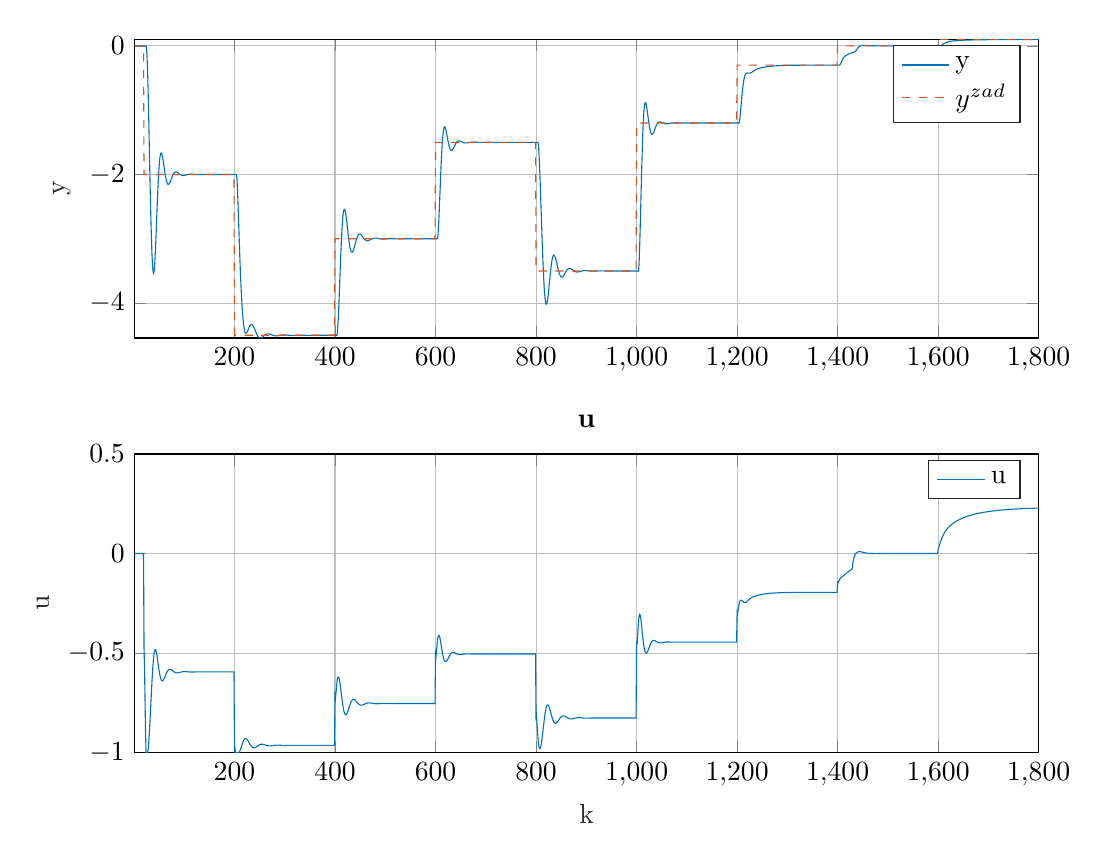
\begin{tikzpicture}

\begin{axis}[%
width=4.521in,
height=1.493in,
at={(0.758in,2.554in)},
scale only axis,
xmin=1,
xmax=1800,
ymin=-4.5419,
ymax=0.1,
ylabel style={font=\color{white!15!black}},
ylabel={y},
axis background/.style={fill=white},
xmajorgrids,
ymajorgrids,
legend style={legend cell align=left, align=left, draw=white!15!black}
]
\addplot [color=mycolor1]
  table[row sep=crcr]{%
1	0\\
2	0\\
3	0\\
4	0\\
5	0\\
6	0\\
7	0\\
8	0\\
9	0\\
10	0\\
11	0\\
12	0\\
13	0\\
14	0\\
15	0\\
16	0\\
17	0\\
18	0\\
19	0\\
20	0\\
21	0\\
22	0\\
23	0\\
24	0\\
25	-0.046722\\
26	-0.17222\\
27	-0.37125\\
28	-0.64589\\
29	-0.98751\\
30	-1.3671\\
31	-1.7547\\
32	-2.1308\\
33	-2.4813\\
34	-2.7944\\
35	-3.06\\
36	-3.2706\\
37	-3.4213\\
38	-3.5099\\
39	-3.5368\\
40	-3.5049\\
41	-3.4197\\
42	-3.2891\\
43	-3.123\\
44	-2.9326\\
45	-2.7299\\
46	-2.5263\\
47	-2.3322\\
48	-2.1559\\
49	-2.0037\\
50	-1.8791\\
51	-1.7839\\
52	-1.7177\\
53	-1.6789\\
54	-1.6647\\
55	-1.6716\\
56	-1.6959\\
57	-1.7335\\
58	-1.7806\\
59	-1.8334\\
60	-1.8884\\
61	-1.9427\\
62	-1.9938\\
63	-2.0396\\
64	-2.0787\\
65	-2.1099\\
66	-2.1328\\
67	-2.1474\\
68	-2.154\\
69	-2.1533\\
70	-2.1462\\
71	-2.1338\\
72	-2.1174\\
73	-2.0983\\
74	-2.0777\\
75	-2.0567\\
76	-2.0364\\
77	-2.0176\\
78	-2.0009\\
79	-1.9869\\
80	-1.9757\\
81	-1.9675\\
82	-1.9622\\
83	-1.9597\\
84	-1.9596\\
85	-1.9616\\
86	-1.9653\\
87	-1.9702\\
88	-1.9759\\
89	-1.9821\\
90	-1.9884\\
91	-1.9944\\
92	-1.9999\\
93	-2.0048\\
94	-2.0088\\
95	-2.0118\\
96	-2.014\\
97	-2.0152\\
98	-2.0156\\
99	-2.0152\\
100	-2.0142\\
101	-2.0127\\
102	-2.0109\\
103	-2.0088\\
104	-2.0066\\
105	-2.0044\\
106	-2.0024\\
107	-2.0005\\
108	-1.9989\\
109	-1.9976\\
110	-1.9966\\
111	-1.9959\\
112	-1.9955\\
113	-1.9954\\
114	-1.9955\\
115	-1.9959\\
116	-1.9963\\
117	-1.9969\\
118	-1.9976\\
119	-1.9983\\
120	-1.999\\
121	-1.9996\\
122	-2.0002\\
123	-2.0007\\
124	-2.001\\
125	-2.0013\\
126	-2.0015\\
127	-2.0016\\
128	-2.0016\\
129	-2.0015\\
130	-2.0014\\
131	-2.0012\\
132	-2.001\\
133	-2.0008\\
134	-2.0006\\
135	-2.0003\\
136	-2.0001\\
137	-1.9999\\
138	-1.9998\\
139	-1.9997\\
140	-1.9996\\
141	-1.9995\\
142	-1.9995\\
143	-1.9995\\
144	-1.9995\\
145	-1.9996\\
146	-1.9996\\
147	-1.9997\\
148	-1.9998\\
149	-1.9998\\
150	-1.9999\\
151	-2\\
152	-2\\
153	-2.0001\\
154	-2.0001\\
155	-2.0002\\
156	-2.0002\\
157	-2.0002\\
158	-2.0002\\
159	-2.0002\\
160	-2.0001\\
161	-2.0001\\
162	-2.0001\\
163	-2.0001\\
164	-2\\
165	-2\\
166	-2\\
167	-2\\
168	-2\\
169	-2\\
170	-2\\
171	-1.9999\\
172	-1.9999\\
173	-1.9999\\
174	-2\\
175	-2\\
176	-2\\
177	-2\\
178	-2\\
179	-2\\
180	-2\\
181	-2\\
182	-2\\
183	-2\\
184	-2\\
185	-2\\
186	-2\\
187	-2\\
188	-2\\
189	-2\\
190	-2\\
191	-2\\
192	-2\\
193	-2\\
194	-2\\
195	-2\\
196	-2\\
197	-2\\
198	-2\\
199	-2\\
200	-2\\
201	-2\\
202	-2\\
203	-2\\
204	-2\\
205	-2.0801\\
206	-2.2427\\
207	-2.4526\\
208	-2.6856\\
209	-2.9234\\
210	-3.1541\\
211	-3.3704\\
212	-3.5682\\
213	-3.7459\\
214	-3.903\\
215	-4.0393\\
216	-4.155\\
217	-4.2505\\
218	-4.3267\\
219	-4.3847\\
220	-4.426\\
221	-4.4525\\
222	-4.4661\\
223	-4.4689\\
224	-4.4632\\
225	-4.451\\
226	-4.4346\\
227	-4.4158\\
228	-4.3963\\
229	-4.3778\\
230	-4.3614\\
231	-4.3482\\
232	-4.3387\\
233	-4.3334\\
234	-4.3325\\
235	-4.3358\\
236	-4.3431\\
237	-4.354\\
238	-4.3678\\
239	-4.3839\\
240	-4.4017\\
241	-4.4205\\
242	-4.4394\\
243	-4.458\\
244	-4.4756\\
245	-4.4917\\
246	-4.5059\\
247	-4.5179\\
248	-4.5275\\
249	-4.5347\\
250	-4.5394\\
251	-4.5418\\
252	-4.5419\\
253	-4.5402\\
254	-4.5368\\
255	-4.532\\
256	-4.5263\\
257	-4.52\\
258	-4.5133\\
259	-4.5066\\
260	-4.5002\\
261	-4.4944\\
262	-4.4892\\
263	-4.4849\\
264	-4.4816\\
265	-4.4792\\
266	-4.4779\\
267	-4.4775\\
268	-4.478\\
269	-4.4793\\
270	-4.4812\\
271	-4.4836\\
272	-4.4865\\
273	-4.4895\\
274	-4.4927\\
275	-4.4958\\
276	-4.4988\\
277	-4.5015\\
278	-4.5038\\
279	-4.5058\\
280	-4.5073\\
281	-4.5084\\
282	-4.5091\\
283	-4.5093\\
284	-4.5091\\
285	-4.5086\\
286	-4.5078\\
287	-4.5067\\
288	-4.5055\\
289	-4.5042\\
290	-4.5028\\
291	-4.5015\\
292	-4.5002\\
293	-4.4991\\
294	-4.4981\\
295	-4.4973\\
296	-4.4966\\
297	-4.4962\\
298	-4.4959\\
299	-4.4958\\
300	-4.496\\
301	-4.4962\\
302	-4.4966\\
303	-4.4971\\
304	-4.4976\\
305	-4.4982\\
306	-4.4988\\
307	-4.4994\\
308	-4.4999\\
309	-4.5004\\
310	-4.5009\\
311	-4.5012\\
312	-4.5015\\
313	-4.5017\\
314	-4.5018\\
315	-4.5018\\
316	-4.5018\\
317	-4.5016\\
318	-4.5015\\
319	-4.5013\\
320	-4.501\\
321	-4.5008\\
322	-4.5005\\
323	-4.5003\\
324	-4.5\\
325	-4.4998\\
326	-4.4996\\
327	-4.4995\\
328	-4.4993\\
329	-4.4993\\
330	-4.4992\\
331	-4.4992\\
332	-4.4992\\
333	-4.4993\\
334	-4.4994\\
335	-4.4995\\
336	-4.4996\\
337	-4.4997\\
338	-4.4998\\
339	-4.4999\\
340	-4.5\\
341	-4.5001\\
342	-4.5002\\
343	-4.5002\\
344	-4.5003\\
345	-4.5003\\
346	-4.5003\\
347	-4.5003\\
348	-4.5003\\
349	-4.5003\\
350	-4.5003\\
351	-4.5002\\
352	-4.5002\\
353	-4.5001\\
354	-4.5001\\
355	-4.5\\
356	-4.5\\
357	-4.5\\
358	-4.4999\\
359	-4.4999\\
360	-4.4999\\
361	-4.4999\\
362	-4.4998\\
363	-4.4998\\
364	-4.4999\\
365	-4.4999\\
366	-4.4999\\
367	-4.4999\\
368	-4.4999\\
369	-4.4999\\
370	-4.5\\
371	-4.5\\
372	-4.5\\
373	-4.5\\
374	-4.5\\
375	-4.5\\
376	-4.5001\\
377	-4.5001\\
378	-4.5001\\
379	-4.5001\\
380	-4.5001\\
381	-4.5001\\
382	-4.5001\\
383	-4.5\\
384	-4.5\\
385	-4.5\\
386	-4.5\\
387	-4.5\\
388	-4.5\\
389	-4.5\\
390	-4.5\\
391	-4.5\\
392	-4.5\\
393	-4.5\\
394	-4.5\\
395	-4.5\\
396	-4.5\\
397	-4.5\\
398	-4.5\\
399	-4.5\\
400	-4.5\\
401	-4.5\\
402	-4.5\\
403	-4.5\\
404	-4.5\\
405	-4.4319\\
406	-4.3057\\
407	-4.143\\
408	-3.9553\\
409	-3.7516\\
410	-3.5418\\
411	-3.3365\\
412	-3.1448\\
413	-2.9739\\
414	-2.8288\\
415	-2.7127\\
416	-2.6269\\
417	-2.5708\\
418	-2.5429\\
419	-2.5405\\
420	-2.5601\\
421	-2.598\\
422	-2.65\\
423	-2.7121\\
424	-2.7804\\
425	-2.851\\
426	-2.9208\\
427	-2.9868\\
428	-3.0467\\
429	-3.0985\\
430	-3.1409\\
431	-3.1731\\
432	-3.1949\\
433	-3.2063\\
434	-3.2081\\
435	-3.2012\\
436	-3.1867\\
437	-3.1662\\
438	-3.1412\\
439	-3.1133\\
440	-3.0839\\
441	-3.0545\\
442	-3.0265\\
443	-3.0007\\
444	-2.9781\\
445	-2.9593\\
446	-2.9446\\
447	-2.9341\\
448	-2.9279\\
449	-2.9256\\
450	-2.9268\\
451	-2.9311\\
452	-2.938\\
453	-2.9468\\
454	-2.9569\\
455	-2.9677\\
456	-2.9786\\
457	-2.9893\\
458	-2.9992\\
459	-3.008\\
460	-3.0155\\
461	-3.0215\\
462	-3.0258\\
463	-3.0286\\
464	-3.0298\\
465	-3.0297\\
466	-3.0282\\
467	-3.0258\\
468	-3.0225\\
469	-3.0187\\
470	-3.0145\\
471	-3.0102\\
472	-3.0059\\
473	-3.0019\\
474	-2.9983\\
475	-2.9952\\
476	-2.9927\\
477	-2.9908\\
478	-2.9895\\
479	-2.9888\\
480	-2.9887\\
481	-2.9891\\
482	-2.9899\\
483	-2.9911\\
484	-2.9925\\
485	-2.994\\
486	-2.9957\\
487	-2.9973\\
488	-2.9989\\
489	-3.0003\\
490	-3.0016\\
491	-3.0026\\
492	-3.0034\\
493	-3.004\\
494	-3.0043\\
495	-3.0044\\
496	-3.0043\\
497	-3.004\\
498	-3.0036\\
499	-3.0031\\
500	-3.0025\\
501	-3.0019\\
502	-3.0012\\
503	-3.0006\\
504	-3.0001\\
505	-2.9996\\
506	-2.9991\\
507	-2.9988\\
508	-2.9985\\
509	-2.9984\\
510	-2.9983\\
511	-2.9983\\
512	-2.9984\\
513	-2.9986\\
514	-2.9987\\
515	-2.999\\
516	-2.9992\\
517	-2.9994\\
518	-2.9997\\
519	-2.9999\\
520	-3.0001\\
521	-3.0003\\
522	-3.0004\\
523	-3.0005\\
524	-3.0006\\
525	-3.0006\\
526	-3.0007\\
527	-3.0006\\
528	-3.0006\\
529	-3.0005\\
530	-3.0004\\
531	-3.0003\\
532	-3.0002\\
533	-3.0001\\
534	-3.0001\\
535	-3\\
536	-2.9999\\
537	-2.9998\\
538	-2.9998\\
539	-2.9998\\
540	-2.9998\\
541	-2.9997\\
542	-2.9998\\
543	-2.9998\\
544	-2.9998\\
545	-2.9998\\
546	-2.9999\\
547	-2.9999\\
548	-2.9999\\
549	-3\\
550	-3\\
551	-3\\
552	-3.0001\\
553	-3.0001\\
554	-3.0001\\
555	-3.0001\\
556	-3.0001\\
557	-3.0001\\
558	-3.0001\\
559	-3.0001\\
560	-3.0001\\
561	-3.0001\\
562	-3\\
563	-3\\
564	-3\\
565	-3\\
566	-3\\
567	-3\\
568	-3\\
569	-3\\
570	-3\\
571	-3\\
572	-3\\
573	-3\\
574	-3\\
575	-3\\
576	-3\\
577	-3\\
578	-3\\
579	-3\\
580	-3\\
581	-3\\
582	-3\\
583	-3\\
584	-3\\
585	-3\\
586	-3\\
587	-3\\
588	-3\\
589	-3\\
590	-3\\
591	-3\\
592	-3\\
593	-3\\
594	-3\\
595	-3\\
596	-3\\
597	-3\\
598	-3\\
599	-3\\
600	-3\\
601	-3\\
602	-3\\
603	-3\\
604	-3\\
605	-2.9262\\
606	-2.7955\\
607	-2.631\\
608	-2.4459\\
609	-2.2501\\
610	-2.0544\\
611	-1.8697\\
612	-1.704\\
613	-1.5627\\
614	-1.4488\\
615	-1.363\\
616	-1.3044\\
617	-1.2709\\
618	-1.2593\\
619	-1.266\\
620	-1.2872\\
621	-1.3192\\
622	-1.3582\\
623	-1.401\\
624	-1.4446\\
625	-1.4866\\
626	-1.5249\\
627	-1.558\\
628	-1.5849\\
629	-1.6051\\
630	-1.6185\\
631	-1.6252\\
632	-1.6259\\
633	-1.6214\\
634	-1.6125\\
635	-1.6003\\
636	-1.5858\\
637	-1.5701\\
638	-1.5541\\
639	-1.5386\\
640	-1.5242\\
641	-1.5115\\
642	-1.5007\\
643	-1.4921\\
644	-1.4858\\
645	-1.4815\\
646	-1.4792\\
647	-1.4787\\
648	-1.4796\\
649	-1.4816\\
650	-1.4845\\
651	-1.488\\
652	-1.4917\\
653	-1.4954\\
654	-1.4989\\
655	-1.502\\
656	-1.5047\\
657	-1.5069\\
658	-1.5084\\
659	-1.5094\\
660	-1.5099\\
661	-1.5098\\
662	-1.5094\\
663	-1.5086\\
664	-1.5076\\
665	-1.5064\\
666	-1.5051\\
667	-1.5039\\
668	-1.5026\\
669	-1.5015\\
670	-1.5005\\
671	-1.4997\\
672	-1.4991\\
673	-1.4986\\
674	-1.4983\\
675	-1.4982\\
676	-1.4982\\
677	-1.4983\\
678	-1.4985\\
679	-1.4987\\
680	-1.499\\
681	-1.4993\\
682	-1.4996\\
683	-1.4999\\
684	-1.5002\\
685	-1.5004\\
686	-1.5006\\
687	-1.5007\\
688	-1.5007\\
689	-1.5008\\
690	-1.5008\\
691	-1.5007\\
692	-1.5007\\
693	-1.5006\\
694	-1.5005\\
695	-1.5004\\
696	-1.5003\\
697	-1.5002\\
698	-1.5001\\
699	-1.5\\
700	-1.5\\
701	-1.4999\\
702	-1.4999\\
703	-1.4999\\
704	-1.4998\\
705	-1.4998\\
706	-1.4999\\
707	-1.4999\\
708	-1.4999\\
709	-1.4999\\
710	-1.4999\\
711	-1.5\\
712	-1.5\\
713	-1.5\\
714	-1.5\\
715	-1.5\\
716	-1.5001\\
717	-1.5001\\
718	-1.5001\\
719	-1.5001\\
720	-1.5001\\
721	-1.5001\\
722	-1.5\\
723	-1.5\\
724	-1.5\\
725	-1.5\\
726	-1.5\\
727	-1.5\\
728	-1.5\\
729	-1.5\\
730	-1.5\\
731	-1.5\\
732	-1.5\\
733	-1.5\\
734	-1.5\\
735	-1.5\\
736	-1.5\\
737	-1.5\\
738	-1.5\\
739	-1.5\\
740	-1.5\\
741	-1.5\\
742	-1.5\\
743	-1.5\\
744	-1.5\\
745	-1.5\\
746	-1.5\\
747	-1.5\\
748	-1.5\\
749	-1.5\\
750	-1.5\\
751	-1.5\\
752	-1.5\\
753	-1.5\\
754	-1.5\\
755	-1.5\\
756	-1.5\\
757	-1.5\\
758	-1.5\\
759	-1.5\\
760	-1.5\\
761	-1.5\\
762	-1.5\\
763	-1.5\\
764	-1.5\\
765	-1.5\\
766	-1.5\\
767	-1.5\\
768	-1.5\\
769	-1.5\\
770	-1.5\\
771	-1.5\\
772	-1.5\\
773	-1.5\\
774	-1.5\\
775	-1.5\\
776	-1.5\\
777	-1.5\\
778	-1.5\\
779	-1.5\\
780	-1.5\\
781	-1.5\\
782	-1.5\\
783	-1.5\\
784	-1.5\\
785	-1.5\\
786	-1.5\\
787	-1.5\\
788	-1.5\\
789	-1.5\\
790	-1.5\\
791	-1.5\\
792	-1.5\\
793	-1.5\\
794	-1.5\\
795	-1.5\\
796	-1.5\\
797	-1.5\\
798	-1.5\\
799	-1.5\\
800	-1.5\\
801	-1.5\\
802	-1.5\\
803	-1.5\\
804	-1.5\\
805	-1.567\\
806	-1.7013\\
807	-1.877\\
808	-2.0809\\
809	-2.3039\\
810	-2.5375\\
811	-2.7728\\
812	-3.0019\\
813	-3.2178\\
814	-3.4145\\
815	-3.5876\\
816	-3.7335\\
817	-3.8499\\
818	-3.9358\\
819	-3.9911\\
820	-4.0172\\
821	-4.0161\\
822	-3.9909\\
823	-3.9454\\
824	-3.8839\\
825	-3.8108\\
826	-3.7307\\
827	-3.6481\\
828	-3.5669\\
829	-3.4908\\
830	-3.4227\\
831	-3.3645\\
832	-3.3179\\
833	-3.2836\\
834	-3.2617\\
835	-3.2518\\
836	-3.2529\\
837	-3.2638\\
838	-3.283\\
839	-3.3087\\
840	-3.3393\\
841	-3.3729\\
842	-3.4078\\
843	-3.4426\\
844	-3.4758\\
845	-3.5062\\
846	-3.533\\
847	-3.5554\\
848	-3.573\\
849	-3.5856\\
850	-3.5932\\
851	-3.596\\
852	-3.5945\\
853	-3.5892\\
854	-3.5807\\
855	-3.5697\\
856	-3.5569\\
857	-3.5432\\
858	-3.5291\\
859	-3.5153\\
860	-3.5024\\
861	-3.4908\\
862	-3.4808\\
863	-3.4727\\
864	-3.4666\\
865	-3.4626\\
866	-3.4605\\
867	-3.4604\\
868	-3.4619\\
869	-3.4648\\
870	-3.4688\\
871	-3.4737\\
872	-3.4792\\
873	-3.4849\\
874	-3.4906\\
875	-3.4961\\
876	-3.5011\\
877	-3.5056\\
878	-3.5093\\
879	-3.5122\\
880	-3.5143\\
881	-3.5156\\
882	-3.5161\\
883	-3.5159\\
884	-3.515\\
885	-3.5136\\
886	-3.5118\\
887	-3.5096\\
888	-3.5074\\
889	-3.505\\
890	-3.5027\\
891	-3.5006\\
892	-3.4986\\
893	-3.497\\
894	-3.4956\\
895	-3.4946\\
896	-3.4939\\
897	-3.4935\\
898	-3.4935\\
899	-3.4937\\
900	-3.4941\\
901	-3.4948\\
902	-3.4956\\
903	-3.4965\\
904	-3.4974\\
905	-3.4984\\
906	-3.4993\\
907	-3.5001\\
908	-3.5009\\
909	-3.5015\\
910	-3.502\\
911	-3.5024\\
912	-3.5026\\
913	-3.5027\\
914	-3.5026\\
915	-3.5025\\
916	-3.5023\\
917	-3.502\\
918	-3.5016\\
919	-3.5012\\
920	-3.5009\\
921	-3.5005\\
922	-3.5001\\
923	-3.4998\\
924	-3.4995\\
925	-3.4993\\
926	-3.4991\\
927	-3.499\\
928	-3.4989\\
929	-3.4989\\
930	-3.4989\\
931	-3.499\\
932	-3.4991\\
933	-3.4993\\
934	-3.4994\\
935	-3.4996\\
936	-3.4997\\
937	-3.4999\\
938	-3.5\\
939	-3.5001\\
940	-3.5002\\
941	-3.5003\\
942	-3.5004\\
943	-3.5004\\
944	-3.5004\\
945	-3.5004\\
946	-3.5004\\
947	-3.5004\\
948	-3.5003\\
949	-3.5003\\
950	-3.5002\\
951	-3.5001\\
952	-3.5001\\
953	-3.5\\
954	-3.5\\
955	-3.4999\\
956	-3.4999\\
957	-3.4999\\
958	-3.4998\\
959	-3.4998\\
960	-3.4998\\
961	-3.4998\\
962	-3.4998\\
963	-3.4999\\
964	-3.4999\\
965	-3.4999\\
966	-3.4999\\
967	-3.5\\
968	-3.5\\
969	-3.5\\
970	-3.5\\
971	-3.5\\
972	-3.5001\\
973	-3.5001\\
974	-3.5001\\
975	-3.5001\\
976	-3.5001\\
977	-3.5001\\
978	-3.5001\\
979	-3.5001\\
980	-3.5\\
981	-3.5\\
982	-3.5\\
983	-3.5\\
984	-3.5\\
985	-3.5\\
986	-3.5\\
987	-3.5\\
988	-3.5\\
989	-3.5\\
990	-3.5\\
991	-3.5\\
992	-3.5\\
993	-3.5\\
994	-3.5\\
995	-3.5\\
996	-3.5\\
997	-3.5\\
998	-3.5\\
999	-3.5\\
1000	-3.5\\
1001	-3.5\\
1002	-3.5\\
1003	-3.5\\
1004	-3.5\\
1005	-3.3746\\
1006	-3.1592\\
1007	-2.8907\\
1008	-2.5911\\
1009	-2.2772\\
1010	-1.9699\\
1011	-1.6876\\
1012	-1.4432\\
1013	-1.2434\\
1014	-1.0904\\
1015	-0.98243\\
1016	-0.91576\\
1017	-0.88498\\
1018	-0.88403\\
1019	-0.90662\\
1020	-0.94665\\
1021	-0.9984\\
1022	-1.0567\\
1023	-1.1171\\
1024	-1.1757\\
1025	-1.2296\\
1026	-1.2766\\
1027	-1.315\\
1028	-1.344\\
1029	-1.3635\\
1030	-1.3737\\
1031	-1.3755\\
1032	-1.3699\\
1033	-1.3582\\
1034	-1.3421\\
1035	-1.3229\\
1036	-1.3021\\
1037	-1.2809\\
1038	-1.2605\\
1039	-1.2416\\
1040	-1.225\\
1041	-1.211\\
1042	-1.1999\\
1043	-1.1916\\
1044	-1.1861\\
1045	-1.183\\
1046	-1.182\\
1047	-1.1828\\
1048	-1.1849\\
1049	-1.1879\\
1050	-1.1915\\
1051	-1.1954\\
1052	-1.1992\\
1053	-1.2028\\
1054	-1.2059\\
1055	-1.2084\\
1056	-1.2103\\
1057	-1.2116\\
1058	-1.2123\\
1059	-1.2124\\
1060	-1.212\\
1061	-1.2112\\
1062	-1.2102\\
1063	-1.2089\\
1064	-1.2075\\
1065	-1.2061\\
1066	-1.2047\\
1067	-1.2035\\
1068	-1.2023\\
1069	-1.2014\\
1070	-1.2006\\
1071	-1.2\\
1072	-1.1996\\
1073	-1.1993\\
1074	-1.1992\\
1075	-1.1992\\
1076	-1.1993\\
1077	-1.1994\\
1078	-1.1996\\
1079	-1.1999\\
1080	-1.2001\\
1081	-1.2003\\
1082	-1.2005\\
1083	-1.2006\\
1084	-1.2008\\
1085	-1.2008\\
1086	-1.2009\\
1087	-1.2009\\
1088	-1.2009\\
1089	-1.2008\\
1090	-1.2007\\
1091	-1.2007\\
1092	-1.2006\\
1093	-1.2005\\
1094	-1.2004\\
1095	-1.2003\\
1096	-1.2002\\
1097	-1.2001\\
1098	-1.2001\\
1099	-1.2\\
1100	-1.2\\
1101	-1.2\\
1102	-1.2\\
1103	-1.2\\
1104	-1.2\\
1105	-1.2\\
1106	-1.2\\
1107	-1.2\\
1108	-1.2\\
1109	-1.2\\
1110	-1.2\\
1111	-1.2001\\
1112	-1.2001\\
1113	-1.2001\\
1114	-1.2001\\
1115	-1.2001\\
1116	-1.2001\\
1117	-1.2001\\
1118	-1.2001\\
1119	-1.2\\
1120	-1.2\\
1121	-1.2\\
1122	-1.2\\
1123	-1.2\\
1124	-1.2\\
1125	-1.2\\
1126	-1.2\\
1127	-1.2\\
1128	-1.2\\
1129	-1.2\\
1130	-1.2\\
1131	-1.2\\
1132	-1.2\\
1133	-1.2\\
1134	-1.2\\
1135	-1.2\\
1136	-1.2\\
1137	-1.2\\
1138	-1.2\\
1139	-1.2\\
1140	-1.2\\
1141	-1.2\\
1142	-1.2\\
1143	-1.2\\
1144	-1.2\\
1145	-1.2\\
1146	-1.2\\
1147	-1.2\\
1148	-1.2\\
1149	-1.2\\
1150	-1.2\\
1151	-1.2\\
1152	-1.2\\
1153	-1.2\\
1154	-1.2\\
1155	-1.2\\
1156	-1.2\\
1157	-1.2\\
1158	-1.2\\
1159	-1.2\\
1160	-1.2\\
1161	-1.2\\
1162	-1.2\\
1163	-1.2\\
1164	-1.2\\
1165	-1.2\\
1166	-1.2\\
1167	-1.2\\
1168	-1.2\\
1169	-1.2\\
1170	-1.2\\
1171	-1.2\\
1172	-1.2\\
1173	-1.2\\
1174	-1.2\\
1175	-1.2\\
1176	-1.2\\
1177	-1.2\\
1178	-1.2\\
1179	-1.2\\
1180	-1.2\\
1181	-1.2\\
1182	-1.2\\
1183	-1.2\\
1184	-1.2\\
1185	-1.2\\
1186	-1.2\\
1187	-1.2\\
1188	-1.2\\
1189	-1.2\\
1190	-1.2\\
1191	-1.2\\
1192	-1.2\\
1193	-1.2\\
1194	-1.2\\
1195	-1.2\\
1196	-1.2\\
1197	-1.2\\
1198	-1.2\\
1199	-1.2\\
1200	-1.2\\
1201	-1.2\\
1202	-1.2\\
1203	-1.2\\
1204	-1.2\\
1205	-1.1595\\
1206	-1.0904\\
1207	-1.0075\\
1208	-0.91874\\
1209	-0.82958\\
1210	-0.7449\\
1211	-0.66863\\
1212	-0.60311\\
1213	-0.54926\\
1214	-0.50692\\
1215	-0.4752\\
1216	-0.45274\\
1217	-0.43794\\
1218	-0.42911\\
1219	-0.42465\\
1220	-0.42312\\
1221	-0.42329\\
1222	-0.42418\\
1223	-0.42504\\
1224	-0.42536\\
1225	-0.42481\\
1226	-0.42326\\
1227	-0.4207\\
1228	-0.41721\\
1229	-0.41295\\
1230	-0.40811\\
1231	-0.40289\\
1232	-0.39746\\
1233	-0.392\\
1234	-0.38665\\
1235	-0.38152\\
1236	-0.37667\\
1237	-0.37216\\
1238	-0.36799\\
1239	-0.36418\\
1240	-0.3607\\
1241	-0.35754\\
1242	-0.35465\\
1243	-0.352\\
1244	-0.34956\\
1245	-0.34729\\
1246	-0.34517\\
1247	-0.34318\\
1248	-0.34129\\
1249	-0.33949\\
1250	-0.33777\\
1251	-0.33611\\
1252	-0.33452\\
1253	-0.33299\\
1254	-0.33152\\
1255	-0.33011\\
1256	-0.32875\\
1257	-0.32745\\
1258	-0.3262\\
1259	-0.32501\\
1260	-0.32388\\
1261	-0.32279\\
1262	-0.32176\\
1263	-0.32077\\
1264	-0.31984\\
1265	-0.31895\\
1266	-0.3181\\
1267	-0.31729\\
1268	-0.31651\\
1269	-0.31578\\
1270	-0.31508\\
1271	-0.31441\\
1272	-0.31377\\
1273	-0.31316\\
1274	-0.31258\\
1275	-0.31203\\
1276	-0.3115\\
1277	-0.31099\\
1278	-0.31051\\
1279	-0.31005\\
1280	-0.3096\\
1281	-0.30918\\
1282	-0.30878\\
1283	-0.30839\\
1284	-0.30802\\
1285	-0.30767\\
1286	-0.30733\\
1287	-0.30701\\
1288	-0.30671\\
1289	-0.30641\\
1290	-0.30613\\
1291	-0.30586\\
1292	-0.30561\\
1293	-0.30536\\
1294	-0.30513\\
1295	-0.3049\\
1296	-0.30469\\
1297	-0.30448\\
1298	-0.30429\\
1299	-0.3041\\
1300	-0.30392\\
1301	-0.30375\\
1302	-0.30359\\
1303	-0.30343\\
1304	-0.30328\\
1305	-0.30314\\
1306	-0.303\\
1307	-0.30287\\
1308	-0.30275\\
1309	-0.30263\\
1310	-0.30251\\
1311	-0.3024\\
1312	-0.3023\\
1313	-0.3022\\
1314	-0.3021\\
1315	-0.30201\\
1316	-0.30192\\
1317	-0.30184\\
1318	-0.30176\\
1319	-0.30168\\
1320	-0.30161\\
1321	-0.30154\\
1322	-0.30147\\
1323	-0.30141\\
1324	-0.30135\\
1325	-0.30129\\
1326	-0.30123\\
1327	-0.30118\\
1328	-0.30113\\
1329	-0.30108\\
1330	-0.30103\\
1331	-0.30099\\
1332	-0.30095\\
1333	-0.3009\\
1334	-0.30087\\
1335	-0.30083\\
1336	-0.30079\\
1337	-0.30076\\
1338	-0.30072\\
1339	-0.30069\\
1340	-0.30066\\
1341	-0.30063\\
1342	-0.30061\\
1343	-0.30058\\
1344	-0.30056\\
1345	-0.30053\\
1346	-0.30051\\
1347	-0.30049\\
1348	-0.30046\\
1349	-0.30044\\
1350	-0.30043\\
1351	-0.30041\\
1352	-0.30039\\
1353	-0.30037\\
1354	-0.30036\\
1355	-0.30034\\
1356	-0.30033\\
1357	-0.30031\\
1358	-0.3003\\
1359	-0.30029\\
1360	-0.30027\\
1361	-0.30026\\
1362	-0.30025\\
1363	-0.30024\\
1364	-0.30023\\
1365	-0.30022\\
1366	-0.30021\\
1367	-0.3002\\
1368	-0.30019\\
1369	-0.30018\\
1370	-0.30018\\
1371	-0.30017\\
1372	-0.30016\\
1373	-0.30015\\
1374	-0.30015\\
1375	-0.30014\\
1376	-0.30013\\
1377	-0.30013\\
1378	-0.30012\\
1379	-0.30012\\
1380	-0.30011\\
1381	-0.30011\\
1382	-0.3001\\
1383	-0.3001\\
1384	-0.30009\\
1385	-0.30009\\
1386	-0.30009\\
1387	-0.30008\\
1388	-0.30008\\
1389	-0.30008\\
1390	-0.30007\\
1391	-0.30007\\
1392	-0.30007\\
1393	-0.30006\\
1394	-0.30006\\
1395	-0.30006\\
1396	-0.30006\\
1397	-0.30005\\
1398	-0.30005\\
1399	-0.30005\\
1400	-0.30005\\
1401	-0.30004\\
1402	-0.30004\\
1403	-0.30004\\
1404	-0.30004\\
1405	-0.2917\\
1406	-0.27707\\
1407	-0.26021\\
1408	-0.24291\\
1409	-0.22617\\
1410	-0.21067\\
1411	-0.19685\\
1412	-0.18488\\
1413	-0.17473\\
1414	-0.16621\\
1415	-0.1591\\
1416	-0.15313\\
1417	-0.14805\\
1418	-0.14361\\
1419	-0.13964\\
1420	-0.13598\\
1421	-0.13252\\
1422	-0.12917\\
1423	-0.12591\\
1424	-0.12269\\
1425	-0.11951\\
1426	-0.11638\\
1427	-0.1133\\
1428	-0.11027\\
1429	-0.10732\\
1430	-0.10445\\
1431	-0.10166\\
1432	-0.098959\\
1433	-0.096353\\
1434	-0.093839\\
1435	-0.089198\\
1436	-0.081196\\
1437	-0.070678\\
1438	-0.059038\\
1439	-0.047265\\
1440	-0.036174\\
1441	-0.026429\\
1442	-0.018324\\
1443	-0.011847\\
1444	-0.0067464\\
1445	-0.0027384\\
1446	0.00037222\\
1447	0.002737\\
1448	0.0044835\\
1449	0.005722\\
1450	0.0065467\\
1451	0.0070376\\
1452	0.0072624\\
1453	0.0072783\\
1454	0.0071332\\
1455	0.0068672\\
1456	0.0065136\\
1457	0.0060996\\
1458	0.0056476\\
1459	0.0051755\\
1460	0.0046977\\
1461	0.0042254\\
1462	0.0037673\\
1463	0.0033298\\
1464	0.0029175\\
1465	0.0025336\\
1466	0.0021798\\
1467	0.0018571\\
1468	0.0015654\\
1469	0.0013042\\
1470	0.0010722\\
1471	0.00086819\\
1472	0.00069025\\
1473	0.00053654\\
1474	0.00040504\\
1475	0.00029373\\
1476	0.00020057\\
1477	0.00012361\\
1478	6.0962e-05\\
1479	1.0834e-05\\
1480	-2.8433e-05\\
1481	-5.8371e-05\\
1482	-8.0383e-05\\
1483	-9.5734e-05\\
1484	-0.00010556\\
1485	-0.00011086\\
1486	-0.00011252\\
1487	-0.00011131\\
1488	-0.0001079\\
1489	-0.00010284\\
1490	-9.6611e-05\\
1491	-8.9615e-05\\
1492	-8.2175e-05\\
1493	-7.4555e-05\\
1494	-6.6964e-05\\
1495	-5.9564e-05\\
1496	-5.2479e-05\\
1497	-4.5795e-05\\
1498	-3.9574e-05\\
1499	-3.3849e-05\\
1500	-2.864e-05\\
1501	-2.3948e-05\\
1502	-1.9762e-05\\
1503	-1.6064e-05\\
1504	-1.2827e-05\\
1505	-1.0022e-05\\
1506	-7.6156e-06\\
1507	-5.5726e-06\\
1508	-3.8581e-06\\
1509	-2.4375e-06\\
1510	-1.2773e-06\\
1511	-3.4556e-07\\
1512	3.8752e-07\\
1513	9.4966e-07\\
1514	1.3662e-06\\
1515	1.6602e-06\\
1516	1.8521e-06\\
1517	1.9604e-06\\
1518	2.0012e-06\\
1519	1.9884e-06\\
1520	1.9343e-06\\
1521	1.8492e-06\\
1522	1.7418e-06\\
1523	1.6195e-06\\
1524	1.4882e-06\\
1525	1.353e-06\\
1526	1.2176e-06\\
1527	1.0852e-06\\
1528	9.5793e-07\\
1529	8.3757e-07\\
1530	7.2525e-07\\
1531	6.2168e-07\\
1532	5.2723e-07\\
1533	4.4197e-07\\
1534	3.6577e-07\\
1535	2.9831e-07\\
1536	2.3916e-07\\
1537	1.8779e-07\\
1538	1.4363e-07\\
1539	1.0605e-07\\
1540	7.443e-08\\
1541	4.8162e-08\\
1542	2.6639e-08\\
1543	9.2902e-09\\
1544	-4.4235e-09\\
1545	-1.5002e-08\\
1546	-2.2905e-08\\
1547	-2.8549e-08\\
1548	-3.2309e-08\\
1549	-3.4518e-08\\
1550	-3.547e-08\\
1551	-3.5424e-08\\
1552	-3.46e-08\\
1553	-3.319e-08\\
1554	-3.1354e-08\\
1555	-2.9228e-08\\
1556	-2.6923e-08\\
1557	-2.453e-08\\
1558	-2.2122e-08\\
1559	-1.9755e-08\\
1560	-1.7474e-08\\
1561	-1.5309e-08\\
1562	-1.3283e-08\\
1563	-1.1411e-08\\
1564	-9.6994e-09\\
1565	-8.1514e-09\\
1566	-6.765e-09\\
1567	-5.5352e-09\\
1568	-4.4547e-09\\
1569	-3.5145e-09\\
1570	-2.7043e-09\\
1571	-2.0135e-09\\
1572	-1.4308e-09\\
1573	-9.4541e-10\\
1574	-5.4646e-10\\
1575	-2.237e-10\\
1576	3.2554e-11\\
1577	2.3135e-10\\
1578	3.8098e-10\\
1579	4.8901e-10\\
1580	5.6225e-10\\
1581	6.0677e-10\\
1582	6.2795e-10\\
1583	6.3049e-10\\
1584	6.1845e-10\\
1585	5.9533e-10\\
1586	5.641e-10\\
1587	5.2724e-10\\
1588	4.8683e-10\\
1589	4.4455e-10\\
1590	4.0175e-10\\
1591	3.5949e-10\\
1592	3.1861e-10\\
1593	2.7969e-10\\
1594	2.4318e-10\\
1595	2.0935e-10\\
1596	1.7835e-10\\
1597	1.5026e-10\\
1598	1.2504e-10\\
1599	1.0263e-10\\
1600	8.2904e-11\\
1601	6.5702e-11\\
1602	5.0848e-11\\
1603	3.8153e-11\\
1604	2.7421e-11\\
1605	0.0014818\\
1606	0.0049077\\
1607	0.00936\\
1608	0.014417\\
1609	0.019762\\
1610	0.025159\\
1611	0.030424\\
1612	0.035423\\
1613	0.040075\\
1614	0.044339\\
1615	0.048206\\
1616	0.051687\\
1617	0.054804\\
1618	0.05759\\
1619	0.060079\\
1620	0.062306\\
1621	0.064303\\
1622	0.0661\\
1623	0.067725\\
1624	0.069201\\
1625	0.070547\\
1626	0.071782\\
1627	0.07292\\
1628	0.073972\\
1629	0.07495\\
1630	0.075862\\
1631	0.076716\\
1632	0.077517\\
1633	0.07827\\
1634	0.078982\\
1635	0.079655\\
1636	0.080292\\
1637	0.080897\\
1638	0.081472\\
1639	0.08202\\
1640	0.082543\\
1641	0.083042\\
1642	0.083519\\
1643	0.083976\\
1644	0.084413\\
1645	0.084833\\
1646	0.085235\\
1647	0.085622\\
1648	0.085994\\
1649	0.086352\\
1650	0.086696\\
1651	0.087028\\
1652	0.087348\\
1653	0.087657\\
1654	0.087955\\
1655	0.088243\\
1656	0.088522\\
1657	0.088791\\
1658	0.089051\\
1659	0.089303\\
1660	0.089547\\
1661	0.089783\\
1662	0.090012\\
1663	0.090235\\
1664	0.09045\\
1665	0.090659\\
1666	0.090862\\
1667	0.091059\\
1668	0.091251\\
1669	0.091437\\
1670	0.091618\\
1671	0.091793\\
1672	0.091964\\
1673	0.092131\\
1674	0.092293\\
1675	0.09245\\
1676	0.092604\\
1677	0.092753\\
1678	0.092899\\
1679	0.093041\\
1680	0.093179\\
1681	0.093314\\
1682	0.093446\\
1683	0.093574\\
1684	0.093699\\
1685	0.093821\\
1686	0.09394\\
1687	0.094057\\
1688	0.09417\\
1689	0.094281\\
1690	0.094389\\
1691	0.094495\\
1692	0.094599\\
1693	0.0947\\
1694	0.094798\\
1695	0.094895\\
1696	0.094989\\
1697	0.095081\\
1698	0.095172\\
1699	0.09526\\
1700	0.095346\\
1701	0.095431\\
1702	0.095513\\
1703	0.095594\\
1704	0.095673\\
1705	0.095751\\
1706	0.095827\\
1707	0.095901\\
1708	0.095974\\
1709	0.096045\\
1710	0.096115\\
1711	0.096183\\
1712	0.09625\\
1713	0.096315\\
1714	0.09638\\
1715	0.096443\\
1716	0.096504\\
1717	0.096565\\
1718	0.096624\\
1719	0.096682\\
1720	0.096739\\
1721	0.096795\\
1722	0.09685\\
1723	0.096903\\
1724	0.096956\\
1725	0.097008\\
1726	0.097058\\
1727	0.097108\\
1728	0.097157\\
1729	0.097205\\
1730	0.097252\\
1731	0.097298\\
1732	0.097343\\
1733	0.097387\\
1734	0.097431\\
1735	0.097474\\
1736	0.097515\\
1737	0.097557\\
1738	0.097597\\
1739	0.097637\\
1740	0.097676\\
1741	0.097714\\
1742	0.097751\\
1743	0.097788\\
1744	0.097825\\
1745	0.09786\\
1746	0.097895\\
1747	0.097929\\
1748	0.097963\\
1749	0.097996\\
1750	0.098029\\
1751	0.098061\\
1752	0.098092\\
1753	0.098123\\
1754	0.098153\\
1755	0.098183\\
1756	0.098212\\
1757	0.098241\\
1758	0.098269\\
1759	0.098297\\
1760	0.098324\\
1761	0.098351\\
1762	0.098377\\
1763	0.098403\\
1764	0.098429\\
1765	0.098454\\
1766	0.098478\\
1767	0.098502\\
1768	0.098526\\
1769	0.09855\\
1770	0.098573\\
1771	0.098595\\
1772	0.098617\\
1773	0.098639\\
1774	0.098661\\
1775	0.098682\\
1776	0.098702\\
1777	0.098723\\
1778	0.098743\\
1779	0.098763\\
1780	0.098782\\
1781	0.098801\\
1782	0.09882\\
1783	0.098838\\
1784	0.098857\\
1785	0.098874\\
1786	0.098892\\
1787	0.098909\\
1788	0.098926\\
1789	0.098943\\
1790	0.098959\\
1791	0.098976\\
1792	0.098991\\
1793	0.099007\\
1794	0.099023\\
1795	0.099038\\
1796	0.099053\\
1797	0.099067\\
1798	0.099082\\
1799	0.099096\\
1800	0.09911\\
};
\addlegendentry{y}

\addplot [color=mycolor2, dashed]
  table[row sep=crcr]{%
1	0\\
2	0\\
3	0\\
4	0\\
5	0\\
6	0\\
7	0\\
8	0\\
9	0\\
10	0\\
11	0\\
12	0\\
13	0\\
14	0\\
15	0\\
16	0\\
17	0\\
18	0\\
19	0\\
20	-2\\
21	-2\\
22	-2\\
23	-2\\
24	-2\\
25	-2\\
26	-2\\
27	-2\\
28	-2\\
29	-2\\
30	-2\\
31	-2\\
32	-2\\
33	-2\\
34	-2\\
35	-2\\
36	-2\\
37	-2\\
38	-2\\
39	-2\\
40	-2\\
41	-2\\
42	-2\\
43	-2\\
44	-2\\
45	-2\\
46	-2\\
47	-2\\
48	-2\\
49	-2\\
50	-2\\
51	-2\\
52	-2\\
53	-2\\
54	-2\\
55	-2\\
56	-2\\
57	-2\\
58	-2\\
59	-2\\
60	-2\\
61	-2\\
62	-2\\
63	-2\\
64	-2\\
65	-2\\
66	-2\\
67	-2\\
68	-2\\
69	-2\\
70	-2\\
71	-2\\
72	-2\\
73	-2\\
74	-2\\
75	-2\\
76	-2\\
77	-2\\
78	-2\\
79	-2\\
80	-2\\
81	-2\\
82	-2\\
83	-2\\
84	-2\\
85	-2\\
86	-2\\
87	-2\\
88	-2\\
89	-2\\
90	-2\\
91	-2\\
92	-2\\
93	-2\\
94	-2\\
95	-2\\
96	-2\\
97	-2\\
98	-2\\
99	-2\\
100	-2\\
101	-2\\
102	-2\\
103	-2\\
104	-2\\
105	-2\\
106	-2\\
107	-2\\
108	-2\\
109	-2\\
110	-2\\
111	-2\\
112	-2\\
113	-2\\
114	-2\\
115	-2\\
116	-2\\
117	-2\\
118	-2\\
119	-2\\
120	-2\\
121	-2\\
122	-2\\
123	-2\\
124	-2\\
125	-2\\
126	-2\\
127	-2\\
128	-2\\
129	-2\\
130	-2\\
131	-2\\
132	-2\\
133	-2\\
134	-2\\
135	-2\\
136	-2\\
137	-2\\
138	-2\\
139	-2\\
140	-2\\
141	-2\\
142	-2\\
143	-2\\
144	-2\\
145	-2\\
146	-2\\
147	-2\\
148	-2\\
149	-2\\
150	-2\\
151	-2\\
152	-2\\
153	-2\\
154	-2\\
155	-2\\
156	-2\\
157	-2\\
158	-2\\
159	-2\\
160	-2\\
161	-2\\
162	-2\\
163	-2\\
164	-2\\
165	-2\\
166	-2\\
167	-2\\
168	-2\\
169	-2\\
170	-2\\
171	-2\\
172	-2\\
173	-2\\
174	-2\\
175	-2\\
176	-2\\
177	-2\\
178	-2\\
179	-2\\
180	-2\\
181	-2\\
182	-2\\
183	-2\\
184	-2\\
185	-2\\
186	-2\\
187	-2\\
188	-2\\
189	-2\\
190	-2\\
191	-2\\
192	-2\\
193	-2\\
194	-2\\
195	-2\\
196	-2\\
197	-2\\
198	-2\\
199	-2\\
200	-4.5\\
201	-4.5\\
202	-4.5\\
203	-4.5\\
204	-4.5\\
205	-4.5\\
206	-4.5\\
207	-4.5\\
208	-4.5\\
209	-4.5\\
210	-4.5\\
211	-4.5\\
212	-4.5\\
213	-4.5\\
214	-4.5\\
215	-4.5\\
216	-4.5\\
217	-4.5\\
218	-4.5\\
219	-4.5\\
220	-4.5\\
221	-4.5\\
222	-4.5\\
223	-4.5\\
224	-4.5\\
225	-4.5\\
226	-4.5\\
227	-4.5\\
228	-4.5\\
229	-4.5\\
230	-4.5\\
231	-4.5\\
232	-4.5\\
233	-4.5\\
234	-4.5\\
235	-4.5\\
236	-4.5\\
237	-4.5\\
238	-4.5\\
239	-4.5\\
240	-4.5\\
241	-4.5\\
242	-4.5\\
243	-4.5\\
244	-4.5\\
245	-4.5\\
246	-4.5\\
247	-4.5\\
248	-4.5\\
249	-4.5\\
250	-4.5\\
251	-4.5\\
252	-4.5\\
253	-4.5\\
254	-4.5\\
255	-4.5\\
256	-4.5\\
257	-4.5\\
258	-4.5\\
259	-4.5\\
260	-4.5\\
261	-4.5\\
262	-4.5\\
263	-4.5\\
264	-4.5\\
265	-4.5\\
266	-4.5\\
267	-4.5\\
268	-4.5\\
269	-4.5\\
270	-4.5\\
271	-4.5\\
272	-4.5\\
273	-4.5\\
274	-4.5\\
275	-4.5\\
276	-4.5\\
277	-4.5\\
278	-4.5\\
279	-4.5\\
280	-4.5\\
281	-4.5\\
282	-4.5\\
283	-4.5\\
284	-4.5\\
285	-4.5\\
286	-4.5\\
287	-4.5\\
288	-4.5\\
289	-4.5\\
290	-4.5\\
291	-4.5\\
292	-4.5\\
293	-4.5\\
294	-4.5\\
295	-4.5\\
296	-4.5\\
297	-4.5\\
298	-4.5\\
299	-4.5\\
300	-4.5\\
301	-4.5\\
302	-4.5\\
303	-4.5\\
304	-4.5\\
305	-4.5\\
306	-4.5\\
307	-4.5\\
308	-4.5\\
309	-4.5\\
310	-4.5\\
311	-4.5\\
312	-4.5\\
313	-4.5\\
314	-4.5\\
315	-4.5\\
316	-4.5\\
317	-4.5\\
318	-4.5\\
319	-4.5\\
320	-4.5\\
321	-4.5\\
322	-4.5\\
323	-4.5\\
324	-4.5\\
325	-4.5\\
326	-4.5\\
327	-4.5\\
328	-4.5\\
329	-4.5\\
330	-4.5\\
331	-4.5\\
332	-4.5\\
333	-4.5\\
334	-4.5\\
335	-4.5\\
336	-4.5\\
337	-4.5\\
338	-4.5\\
339	-4.5\\
340	-4.5\\
341	-4.5\\
342	-4.5\\
343	-4.5\\
344	-4.5\\
345	-4.5\\
346	-4.5\\
347	-4.5\\
348	-4.5\\
349	-4.5\\
350	-4.5\\
351	-4.5\\
352	-4.5\\
353	-4.5\\
354	-4.5\\
355	-4.5\\
356	-4.5\\
357	-4.5\\
358	-4.5\\
359	-4.5\\
360	-4.5\\
361	-4.5\\
362	-4.5\\
363	-4.5\\
364	-4.5\\
365	-4.5\\
366	-4.5\\
367	-4.5\\
368	-4.5\\
369	-4.5\\
370	-4.5\\
371	-4.5\\
372	-4.5\\
373	-4.5\\
374	-4.5\\
375	-4.5\\
376	-4.5\\
377	-4.5\\
378	-4.5\\
379	-4.5\\
380	-4.5\\
381	-4.5\\
382	-4.5\\
383	-4.5\\
384	-4.5\\
385	-4.5\\
386	-4.5\\
387	-4.5\\
388	-4.5\\
389	-4.5\\
390	-4.5\\
391	-4.5\\
392	-4.5\\
393	-4.5\\
394	-4.5\\
395	-4.5\\
396	-4.5\\
397	-4.5\\
398	-4.5\\
399	-4.5\\
400	-3\\
401	-3\\
402	-3\\
403	-3\\
404	-3\\
405	-3\\
406	-3\\
407	-3\\
408	-3\\
409	-3\\
410	-3\\
411	-3\\
412	-3\\
413	-3\\
414	-3\\
415	-3\\
416	-3\\
417	-3\\
418	-3\\
419	-3\\
420	-3\\
421	-3\\
422	-3\\
423	-3\\
424	-3\\
425	-3\\
426	-3\\
427	-3\\
428	-3\\
429	-3\\
430	-3\\
431	-3\\
432	-3\\
433	-3\\
434	-3\\
435	-3\\
436	-3\\
437	-3\\
438	-3\\
439	-3\\
440	-3\\
441	-3\\
442	-3\\
443	-3\\
444	-3\\
445	-3\\
446	-3\\
447	-3\\
448	-3\\
449	-3\\
450	-3\\
451	-3\\
452	-3\\
453	-3\\
454	-3\\
455	-3\\
456	-3\\
457	-3\\
458	-3\\
459	-3\\
460	-3\\
461	-3\\
462	-3\\
463	-3\\
464	-3\\
465	-3\\
466	-3\\
467	-3\\
468	-3\\
469	-3\\
470	-3\\
471	-3\\
472	-3\\
473	-3\\
474	-3\\
475	-3\\
476	-3\\
477	-3\\
478	-3\\
479	-3\\
480	-3\\
481	-3\\
482	-3\\
483	-3\\
484	-3\\
485	-3\\
486	-3\\
487	-3\\
488	-3\\
489	-3\\
490	-3\\
491	-3\\
492	-3\\
493	-3\\
494	-3\\
495	-3\\
496	-3\\
497	-3\\
498	-3\\
499	-3\\
500	-3\\
501	-3\\
502	-3\\
503	-3\\
504	-3\\
505	-3\\
506	-3\\
507	-3\\
508	-3\\
509	-3\\
510	-3\\
511	-3\\
512	-3\\
513	-3\\
514	-3\\
515	-3\\
516	-3\\
517	-3\\
518	-3\\
519	-3\\
520	-3\\
521	-3\\
522	-3\\
523	-3\\
524	-3\\
525	-3\\
526	-3\\
527	-3\\
528	-3\\
529	-3\\
530	-3\\
531	-3\\
532	-3\\
533	-3\\
534	-3\\
535	-3\\
536	-3\\
537	-3\\
538	-3\\
539	-3\\
540	-3\\
541	-3\\
542	-3\\
543	-3\\
544	-3\\
545	-3\\
546	-3\\
547	-3\\
548	-3\\
549	-3\\
550	-3\\
551	-3\\
552	-3\\
553	-3\\
554	-3\\
555	-3\\
556	-3\\
557	-3\\
558	-3\\
559	-3\\
560	-3\\
561	-3\\
562	-3\\
563	-3\\
564	-3\\
565	-3\\
566	-3\\
567	-3\\
568	-3\\
569	-3\\
570	-3\\
571	-3\\
572	-3\\
573	-3\\
574	-3\\
575	-3\\
576	-3\\
577	-3\\
578	-3\\
579	-3\\
580	-3\\
581	-3\\
582	-3\\
583	-3\\
584	-3\\
585	-3\\
586	-3\\
587	-3\\
588	-3\\
589	-3\\
590	-3\\
591	-3\\
592	-3\\
593	-3\\
594	-3\\
595	-3\\
596	-3\\
597	-3\\
598	-3\\
599	-3\\
600	-1.5\\
601	-1.5\\
602	-1.5\\
603	-1.5\\
604	-1.5\\
605	-1.5\\
606	-1.5\\
607	-1.5\\
608	-1.5\\
609	-1.5\\
610	-1.5\\
611	-1.5\\
612	-1.5\\
613	-1.5\\
614	-1.5\\
615	-1.5\\
616	-1.5\\
617	-1.5\\
618	-1.5\\
619	-1.5\\
620	-1.5\\
621	-1.5\\
622	-1.5\\
623	-1.5\\
624	-1.5\\
625	-1.5\\
626	-1.5\\
627	-1.5\\
628	-1.5\\
629	-1.5\\
630	-1.5\\
631	-1.5\\
632	-1.5\\
633	-1.5\\
634	-1.5\\
635	-1.5\\
636	-1.5\\
637	-1.5\\
638	-1.5\\
639	-1.5\\
640	-1.5\\
641	-1.5\\
642	-1.5\\
643	-1.5\\
644	-1.5\\
645	-1.5\\
646	-1.5\\
647	-1.5\\
648	-1.5\\
649	-1.5\\
650	-1.5\\
651	-1.5\\
652	-1.5\\
653	-1.5\\
654	-1.5\\
655	-1.5\\
656	-1.5\\
657	-1.5\\
658	-1.5\\
659	-1.5\\
660	-1.5\\
661	-1.5\\
662	-1.5\\
663	-1.5\\
664	-1.5\\
665	-1.5\\
666	-1.5\\
667	-1.5\\
668	-1.5\\
669	-1.5\\
670	-1.5\\
671	-1.5\\
672	-1.5\\
673	-1.5\\
674	-1.5\\
675	-1.5\\
676	-1.5\\
677	-1.5\\
678	-1.5\\
679	-1.5\\
680	-1.5\\
681	-1.5\\
682	-1.5\\
683	-1.5\\
684	-1.5\\
685	-1.5\\
686	-1.5\\
687	-1.5\\
688	-1.5\\
689	-1.5\\
690	-1.5\\
691	-1.5\\
692	-1.5\\
693	-1.5\\
694	-1.5\\
695	-1.5\\
696	-1.5\\
697	-1.5\\
698	-1.5\\
699	-1.5\\
700	-1.5\\
701	-1.5\\
702	-1.5\\
703	-1.5\\
704	-1.5\\
705	-1.5\\
706	-1.5\\
707	-1.5\\
708	-1.5\\
709	-1.5\\
710	-1.5\\
711	-1.5\\
712	-1.5\\
713	-1.5\\
714	-1.5\\
715	-1.5\\
716	-1.5\\
717	-1.5\\
718	-1.5\\
719	-1.5\\
720	-1.5\\
721	-1.5\\
722	-1.5\\
723	-1.5\\
724	-1.5\\
725	-1.5\\
726	-1.5\\
727	-1.5\\
728	-1.5\\
729	-1.5\\
730	-1.5\\
731	-1.5\\
732	-1.5\\
733	-1.5\\
734	-1.5\\
735	-1.5\\
736	-1.5\\
737	-1.5\\
738	-1.5\\
739	-1.5\\
740	-1.5\\
741	-1.5\\
742	-1.5\\
743	-1.5\\
744	-1.5\\
745	-1.5\\
746	-1.5\\
747	-1.5\\
748	-1.5\\
749	-1.5\\
750	-1.5\\
751	-1.5\\
752	-1.5\\
753	-1.5\\
754	-1.5\\
755	-1.5\\
756	-1.5\\
757	-1.5\\
758	-1.5\\
759	-1.5\\
760	-1.5\\
761	-1.5\\
762	-1.5\\
763	-1.5\\
764	-1.5\\
765	-1.5\\
766	-1.5\\
767	-1.5\\
768	-1.5\\
769	-1.5\\
770	-1.5\\
771	-1.5\\
772	-1.5\\
773	-1.5\\
774	-1.5\\
775	-1.5\\
776	-1.5\\
777	-1.5\\
778	-1.5\\
779	-1.5\\
780	-1.5\\
781	-1.5\\
782	-1.5\\
783	-1.5\\
784	-1.5\\
785	-1.5\\
786	-1.5\\
787	-1.5\\
788	-1.5\\
789	-1.5\\
790	-1.5\\
791	-1.5\\
792	-1.5\\
793	-1.5\\
794	-1.5\\
795	-1.5\\
796	-1.5\\
797	-1.5\\
798	-1.5\\
799	-1.5\\
800	-3.5\\
801	-3.5\\
802	-3.5\\
803	-3.5\\
804	-3.5\\
805	-3.5\\
806	-3.5\\
807	-3.5\\
808	-3.5\\
809	-3.5\\
810	-3.5\\
811	-3.5\\
812	-3.5\\
813	-3.5\\
814	-3.5\\
815	-3.5\\
816	-3.5\\
817	-3.5\\
818	-3.5\\
819	-3.5\\
820	-3.5\\
821	-3.5\\
822	-3.5\\
823	-3.5\\
824	-3.5\\
825	-3.5\\
826	-3.5\\
827	-3.5\\
828	-3.5\\
829	-3.5\\
830	-3.5\\
831	-3.5\\
832	-3.5\\
833	-3.5\\
834	-3.5\\
835	-3.5\\
836	-3.5\\
837	-3.5\\
838	-3.5\\
839	-3.5\\
840	-3.5\\
841	-3.5\\
842	-3.5\\
843	-3.5\\
844	-3.5\\
845	-3.5\\
846	-3.5\\
847	-3.5\\
848	-3.5\\
849	-3.5\\
850	-3.5\\
851	-3.5\\
852	-3.5\\
853	-3.5\\
854	-3.5\\
855	-3.5\\
856	-3.5\\
857	-3.5\\
858	-3.5\\
859	-3.5\\
860	-3.5\\
861	-3.5\\
862	-3.5\\
863	-3.5\\
864	-3.5\\
865	-3.5\\
866	-3.5\\
867	-3.5\\
868	-3.5\\
869	-3.5\\
870	-3.5\\
871	-3.5\\
872	-3.5\\
873	-3.5\\
874	-3.5\\
875	-3.5\\
876	-3.5\\
877	-3.5\\
878	-3.5\\
879	-3.5\\
880	-3.5\\
881	-3.5\\
882	-3.5\\
883	-3.5\\
884	-3.5\\
885	-3.5\\
886	-3.5\\
887	-3.5\\
888	-3.5\\
889	-3.5\\
890	-3.5\\
891	-3.5\\
892	-3.5\\
893	-3.5\\
894	-3.5\\
895	-3.5\\
896	-3.5\\
897	-3.5\\
898	-3.5\\
899	-3.5\\
900	-3.5\\
901	-3.5\\
902	-3.5\\
903	-3.5\\
904	-3.5\\
905	-3.5\\
906	-3.5\\
907	-3.5\\
908	-3.5\\
909	-3.5\\
910	-3.5\\
911	-3.5\\
912	-3.5\\
913	-3.5\\
914	-3.5\\
915	-3.5\\
916	-3.5\\
917	-3.5\\
918	-3.5\\
919	-3.5\\
920	-3.5\\
921	-3.5\\
922	-3.5\\
923	-3.5\\
924	-3.5\\
925	-3.5\\
926	-3.5\\
927	-3.5\\
928	-3.5\\
929	-3.5\\
930	-3.5\\
931	-3.5\\
932	-3.5\\
933	-3.5\\
934	-3.5\\
935	-3.5\\
936	-3.5\\
937	-3.5\\
938	-3.5\\
939	-3.5\\
940	-3.5\\
941	-3.5\\
942	-3.5\\
943	-3.5\\
944	-3.5\\
945	-3.5\\
946	-3.5\\
947	-3.5\\
948	-3.5\\
949	-3.5\\
950	-3.5\\
951	-3.5\\
952	-3.5\\
953	-3.5\\
954	-3.5\\
955	-3.5\\
956	-3.5\\
957	-3.5\\
958	-3.5\\
959	-3.5\\
960	-3.5\\
961	-3.5\\
962	-3.5\\
963	-3.5\\
964	-3.5\\
965	-3.5\\
966	-3.5\\
967	-3.5\\
968	-3.5\\
969	-3.5\\
970	-3.5\\
971	-3.5\\
972	-3.5\\
973	-3.5\\
974	-3.5\\
975	-3.5\\
976	-3.5\\
977	-3.5\\
978	-3.5\\
979	-3.5\\
980	-3.5\\
981	-3.5\\
982	-3.5\\
983	-3.5\\
984	-3.5\\
985	-3.5\\
986	-3.5\\
987	-3.5\\
988	-3.5\\
989	-3.5\\
990	-3.5\\
991	-3.5\\
992	-3.5\\
993	-3.5\\
994	-3.5\\
995	-3.5\\
996	-3.5\\
997	-3.5\\
998	-3.5\\
999	-3.5\\
1000	-1.2\\
1001	-1.2\\
1002	-1.2\\
1003	-1.2\\
1004	-1.2\\
1005	-1.2\\
1006	-1.2\\
1007	-1.2\\
1008	-1.2\\
1009	-1.2\\
1010	-1.2\\
1011	-1.2\\
1012	-1.2\\
1013	-1.2\\
1014	-1.2\\
1015	-1.2\\
1016	-1.2\\
1017	-1.2\\
1018	-1.2\\
1019	-1.2\\
1020	-1.2\\
1021	-1.2\\
1022	-1.2\\
1023	-1.2\\
1024	-1.2\\
1025	-1.2\\
1026	-1.2\\
1027	-1.2\\
1028	-1.2\\
1029	-1.2\\
1030	-1.2\\
1031	-1.2\\
1032	-1.2\\
1033	-1.2\\
1034	-1.2\\
1035	-1.2\\
1036	-1.2\\
1037	-1.2\\
1038	-1.2\\
1039	-1.2\\
1040	-1.2\\
1041	-1.2\\
1042	-1.2\\
1043	-1.2\\
1044	-1.2\\
1045	-1.2\\
1046	-1.2\\
1047	-1.2\\
1048	-1.2\\
1049	-1.2\\
1050	-1.2\\
1051	-1.2\\
1052	-1.2\\
1053	-1.2\\
1054	-1.2\\
1055	-1.2\\
1056	-1.2\\
1057	-1.2\\
1058	-1.2\\
1059	-1.2\\
1060	-1.2\\
1061	-1.2\\
1062	-1.2\\
1063	-1.2\\
1064	-1.2\\
1065	-1.2\\
1066	-1.2\\
1067	-1.2\\
1068	-1.2\\
1069	-1.2\\
1070	-1.2\\
1071	-1.2\\
1072	-1.2\\
1073	-1.2\\
1074	-1.2\\
1075	-1.2\\
1076	-1.2\\
1077	-1.2\\
1078	-1.2\\
1079	-1.2\\
1080	-1.2\\
1081	-1.2\\
1082	-1.2\\
1083	-1.2\\
1084	-1.2\\
1085	-1.2\\
1086	-1.2\\
1087	-1.2\\
1088	-1.2\\
1089	-1.2\\
1090	-1.2\\
1091	-1.2\\
1092	-1.2\\
1093	-1.2\\
1094	-1.2\\
1095	-1.2\\
1096	-1.2\\
1097	-1.2\\
1098	-1.2\\
1099	-1.2\\
1100	-1.2\\
1101	-1.2\\
1102	-1.2\\
1103	-1.2\\
1104	-1.2\\
1105	-1.2\\
1106	-1.2\\
1107	-1.2\\
1108	-1.2\\
1109	-1.2\\
1110	-1.2\\
1111	-1.2\\
1112	-1.2\\
1113	-1.2\\
1114	-1.2\\
1115	-1.2\\
1116	-1.2\\
1117	-1.2\\
1118	-1.2\\
1119	-1.2\\
1120	-1.2\\
1121	-1.2\\
1122	-1.2\\
1123	-1.2\\
1124	-1.2\\
1125	-1.2\\
1126	-1.2\\
1127	-1.2\\
1128	-1.2\\
1129	-1.2\\
1130	-1.2\\
1131	-1.2\\
1132	-1.2\\
1133	-1.2\\
1134	-1.2\\
1135	-1.2\\
1136	-1.2\\
1137	-1.2\\
1138	-1.2\\
1139	-1.2\\
1140	-1.2\\
1141	-1.2\\
1142	-1.2\\
1143	-1.2\\
1144	-1.2\\
1145	-1.2\\
1146	-1.2\\
1147	-1.2\\
1148	-1.2\\
1149	-1.2\\
1150	-1.2\\
1151	-1.2\\
1152	-1.2\\
1153	-1.2\\
1154	-1.2\\
1155	-1.2\\
1156	-1.2\\
1157	-1.2\\
1158	-1.2\\
1159	-1.2\\
1160	-1.2\\
1161	-1.2\\
1162	-1.2\\
1163	-1.2\\
1164	-1.2\\
1165	-1.2\\
1166	-1.2\\
1167	-1.2\\
1168	-1.2\\
1169	-1.2\\
1170	-1.2\\
1171	-1.2\\
1172	-1.2\\
1173	-1.2\\
1174	-1.2\\
1175	-1.2\\
1176	-1.2\\
1177	-1.2\\
1178	-1.2\\
1179	-1.2\\
1180	-1.2\\
1181	-1.2\\
1182	-1.2\\
1183	-1.2\\
1184	-1.2\\
1185	-1.2\\
1186	-1.2\\
1187	-1.2\\
1188	-1.2\\
1189	-1.2\\
1190	-1.2\\
1191	-1.2\\
1192	-1.2\\
1193	-1.2\\
1194	-1.2\\
1195	-1.2\\
1196	-1.2\\
1197	-1.2\\
1198	-1.2\\
1199	-1.2\\
1200	-0.3\\
1201	-0.3\\
1202	-0.3\\
1203	-0.3\\
1204	-0.3\\
1205	-0.3\\
1206	-0.3\\
1207	-0.3\\
1208	-0.3\\
1209	-0.3\\
1210	-0.3\\
1211	-0.3\\
1212	-0.3\\
1213	-0.3\\
1214	-0.3\\
1215	-0.3\\
1216	-0.3\\
1217	-0.3\\
1218	-0.3\\
1219	-0.3\\
1220	-0.3\\
1221	-0.3\\
1222	-0.3\\
1223	-0.3\\
1224	-0.3\\
1225	-0.3\\
1226	-0.3\\
1227	-0.3\\
1228	-0.3\\
1229	-0.3\\
1230	-0.3\\
1231	-0.3\\
1232	-0.3\\
1233	-0.3\\
1234	-0.3\\
1235	-0.3\\
1236	-0.3\\
1237	-0.3\\
1238	-0.3\\
1239	-0.3\\
1240	-0.3\\
1241	-0.3\\
1242	-0.3\\
1243	-0.3\\
1244	-0.3\\
1245	-0.3\\
1246	-0.3\\
1247	-0.3\\
1248	-0.3\\
1249	-0.3\\
1250	-0.3\\
1251	-0.3\\
1252	-0.3\\
1253	-0.3\\
1254	-0.3\\
1255	-0.3\\
1256	-0.3\\
1257	-0.3\\
1258	-0.3\\
1259	-0.3\\
1260	-0.3\\
1261	-0.3\\
1262	-0.3\\
1263	-0.3\\
1264	-0.3\\
1265	-0.3\\
1266	-0.3\\
1267	-0.3\\
1268	-0.3\\
1269	-0.3\\
1270	-0.3\\
1271	-0.3\\
1272	-0.3\\
1273	-0.3\\
1274	-0.3\\
1275	-0.3\\
1276	-0.3\\
1277	-0.3\\
1278	-0.3\\
1279	-0.3\\
1280	-0.3\\
1281	-0.3\\
1282	-0.3\\
1283	-0.3\\
1284	-0.3\\
1285	-0.3\\
1286	-0.3\\
1287	-0.3\\
1288	-0.3\\
1289	-0.3\\
1290	-0.3\\
1291	-0.3\\
1292	-0.3\\
1293	-0.3\\
1294	-0.3\\
1295	-0.3\\
1296	-0.3\\
1297	-0.3\\
1298	-0.3\\
1299	-0.3\\
1300	-0.3\\
1301	-0.3\\
1302	-0.3\\
1303	-0.3\\
1304	-0.3\\
1305	-0.3\\
1306	-0.3\\
1307	-0.3\\
1308	-0.3\\
1309	-0.3\\
1310	-0.3\\
1311	-0.3\\
1312	-0.3\\
1313	-0.3\\
1314	-0.3\\
1315	-0.3\\
1316	-0.3\\
1317	-0.3\\
1318	-0.3\\
1319	-0.3\\
1320	-0.3\\
1321	-0.3\\
1322	-0.3\\
1323	-0.3\\
1324	-0.3\\
1325	-0.3\\
1326	-0.3\\
1327	-0.3\\
1328	-0.3\\
1329	-0.3\\
1330	-0.3\\
1331	-0.3\\
1332	-0.3\\
1333	-0.3\\
1334	-0.3\\
1335	-0.3\\
1336	-0.3\\
1337	-0.3\\
1338	-0.3\\
1339	-0.3\\
1340	-0.3\\
1341	-0.3\\
1342	-0.3\\
1343	-0.3\\
1344	-0.3\\
1345	-0.3\\
1346	-0.3\\
1347	-0.3\\
1348	-0.3\\
1349	-0.3\\
1350	-0.3\\
1351	-0.3\\
1352	-0.3\\
1353	-0.3\\
1354	-0.3\\
1355	-0.3\\
1356	-0.3\\
1357	-0.3\\
1358	-0.3\\
1359	-0.3\\
1360	-0.3\\
1361	-0.3\\
1362	-0.3\\
1363	-0.3\\
1364	-0.3\\
1365	-0.3\\
1366	-0.3\\
1367	-0.3\\
1368	-0.3\\
1369	-0.3\\
1370	-0.3\\
1371	-0.3\\
1372	-0.3\\
1373	-0.3\\
1374	-0.3\\
1375	-0.3\\
1376	-0.3\\
1377	-0.3\\
1378	-0.3\\
1379	-0.3\\
1380	-0.3\\
1381	-0.3\\
1382	-0.3\\
1383	-0.3\\
1384	-0.3\\
1385	-0.3\\
1386	-0.3\\
1387	-0.3\\
1388	-0.3\\
1389	-0.3\\
1390	-0.3\\
1391	-0.3\\
1392	-0.3\\
1393	-0.3\\
1394	-0.3\\
1395	-0.3\\
1396	-0.3\\
1397	-0.3\\
1398	-0.3\\
1399	-0.3\\
1400	0\\
1401	0\\
1402	0\\
1403	0\\
1404	0\\
1405	0\\
1406	0\\
1407	0\\
1408	0\\
1409	0\\
1410	0\\
1411	0\\
1412	0\\
1413	0\\
1414	0\\
1415	0\\
1416	0\\
1417	0\\
1418	0\\
1419	0\\
1420	0\\
1421	0\\
1422	0\\
1423	0\\
1424	0\\
1425	0\\
1426	0\\
1427	0\\
1428	0\\
1429	0\\
1430	0\\
1431	0\\
1432	0\\
1433	0\\
1434	0\\
1435	0\\
1436	0\\
1437	0\\
1438	0\\
1439	0\\
1440	0\\
1441	0\\
1442	0\\
1443	0\\
1444	0\\
1445	0\\
1446	0\\
1447	0\\
1448	0\\
1449	0\\
1450	0\\
1451	0\\
1452	0\\
1453	0\\
1454	0\\
1455	0\\
1456	0\\
1457	0\\
1458	0\\
1459	0\\
1460	0\\
1461	0\\
1462	0\\
1463	0\\
1464	0\\
1465	0\\
1466	0\\
1467	0\\
1468	0\\
1469	0\\
1470	0\\
1471	0\\
1472	0\\
1473	0\\
1474	0\\
1475	0\\
1476	0\\
1477	0\\
1478	0\\
1479	0\\
1480	0\\
1481	0\\
1482	0\\
1483	0\\
1484	0\\
1485	0\\
1486	0\\
1487	0\\
1488	0\\
1489	0\\
1490	0\\
1491	0\\
1492	0\\
1493	0\\
1494	0\\
1495	0\\
1496	0\\
1497	0\\
1498	0\\
1499	0\\
1500	0\\
1501	0\\
1502	0\\
1503	0\\
1504	0\\
1505	0\\
1506	0\\
1507	0\\
1508	0\\
1509	0\\
1510	0\\
1511	0\\
1512	0\\
1513	0\\
1514	0\\
1515	0\\
1516	0\\
1517	0\\
1518	0\\
1519	0\\
1520	0\\
1521	0\\
1522	0\\
1523	0\\
1524	0\\
1525	0\\
1526	0\\
1527	0\\
1528	0\\
1529	0\\
1530	0\\
1531	0\\
1532	0\\
1533	0\\
1534	0\\
1535	0\\
1536	0\\
1537	0\\
1538	0\\
1539	0\\
1540	0\\
1541	0\\
1542	0\\
1543	0\\
1544	0\\
1545	0\\
1546	0\\
1547	0\\
1548	0\\
1549	0\\
1550	0\\
1551	0\\
1552	0\\
1553	0\\
1554	0\\
1555	0\\
1556	0\\
1557	0\\
1558	0\\
1559	0\\
1560	0\\
1561	0\\
1562	0\\
1563	0\\
1564	0\\
1565	0\\
1566	0\\
1567	0\\
1568	0\\
1569	0\\
1570	0\\
1571	0\\
1572	0\\
1573	0\\
1574	0\\
1575	0\\
1576	0\\
1577	0\\
1578	0\\
1579	0\\
1580	0\\
1581	0\\
1582	0\\
1583	0\\
1584	0\\
1585	0\\
1586	0\\
1587	0\\
1588	0\\
1589	0\\
1590	0\\
1591	0\\
1592	0\\
1593	0\\
1594	0\\
1595	0\\
1596	0\\
1597	0\\
1598	0\\
1599	0\\
1600	0.1\\
1601	0.1\\
1602	0.1\\
1603	0.1\\
1604	0.1\\
1605	0.1\\
1606	0.1\\
1607	0.1\\
1608	0.1\\
1609	0.1\\
1610	0.1\\
1611	0.1\\
1612	0.1\\
1613	0.1\\
1614	0.1\\
1615	0.1\\
1616	0.1\\
1617	0.1\\
1618	0.1\\
1619	0.1\\
1620	0.1\\
1621	0.1\\
1622	0.1\\
1623	0.1\\
1624	0.1\\
1625	0.1\\
1626	0.1\\
1627	0.1\\
1628	0.1\\
1629	0.1\\
1630	0.1\\
1631	0.1\\
1632	0.1\\
1633	0.1\\
1634	0.1\\
1635	0.1\\
1636	0.1\\
1637	0.1\\
1638	0.1\\
1639	0.1\\
1640	0.1\\
1641	0.1\\
1642	0.1\\
1643	0.1\\
1644	0.1\\
1645	0.1\\
1646	0.1\\
1647	0.1\\
1648	0.1\\
1649	0.1\\
1650	0.1\\
1651	0.1\\
1652	0.1\\
1653	0.1\\
1654	0.1\\
1655	0.1\\
1656	0.1\\
1657	0.1\\
1658	0.1\\
1659	0.1\\
1660	0.1\\
1661	0.1\\
1662	0.1\\
1663	0.1\\
1664	0.1\\
1665	0.1\\
1666	0.1\\
1667	0.1\\
1668	0.1\\
1669	0.1\\
1670	0.1\\
1671	0.1\\
1672	0.1\\
1673	0.1\\
1674	0.1\\
1675	0.1\\
1676	0.1\\
1677	0.1\\
1678	0.1\\
1679	0.1\\
1680	0.1\\
1681	0.1\\
1682	0.1\\
1683	0.1\\
1684	0.1\\
1685	0.1\\
1686	0.1\\
1687	0.1\\
1688	0.1\\
1689	0.1\\
1690	0.1\\
1691	0.1\\
1692	0.1\\
1693	0.1\\
1694	0.1\\
1695	0.1\\
1696	0.1\\
1697	0.1\\
1698	0.1\\
1699	0.1\\
1700	0.1\\
1701	0.1\\
1702	0.1\\
1703	0.1\\
1704	0.1\\
1705	0.1\\
1706	0.1\\
1707	0.1\\
1708	0.1\\
1709	0.1\\
1710	0.1\\
1711	0.1\\
1712	0.1\\
1713	0.1\\
1714	0.1\\
1715	0.1\\
1716	0.1\\
1717	0.1\\
1718	0.1\\
1719	0.1\\
1720	0.1\\
1721	0.1\\
1722	0.1\\
1723	0.1\\
1724	0.1\\
1725	0.1\\
1726	0.1\\
1727	0.1\\
1728	0.1\\
1729	0.1\\
1730	0.1\\
1731	0.1\\
1732	0.1\\
1733	0.1\\
1734	0.1\\
1735	0.1\\
1736	0.1\\
1737	0.1\\
1738	0.1\\
1739	0.1\\
1740	0.1\\
1741	0.1\\
1742	0.1\\
1743	0.1\\
1744	0.1\\
1745	0.1\\
1746	0.1\\
1747	0.1\\
1748	0.1\\
1749	0.1\\
1750	0.1\\
1751	0.1\\
1752	0.1\\
1753	0.1\\
1754	0.1\\
1755	0.1\\
1756	0.1\\
1757	0.1\\
1758	0.1\\
1759	0.1\\
1760	0.1\\
1761	0.1\\
1762	0.1\\
1763	0.1\\
1764	0.1\\
1765	0.1\\
1766	0.1\\
1767	0.1\\
1768	0.1\\
1769	0.1\\
1770	0.1\\
1771	0.1\\
1772	0.1\\
1773	0.1\\
1774	0.1\\
1775	0.1\\
1776	0.1\\
1777	0.1\\
1778	0.1\\
1779	0.1\\
1780	0.1\\
1781	0.1\\
1782	0.1\\
1783	0.1\\
1784	0.1\\
1785	0.1\\
1786	0.1\\
1787	0.1\\
1788	0.1\\
1789	0.1\\
1790	0.1\\
1791	0.1\\
1792	0.1\\
1793	0.1\\
1794	0.1\\
1795	0.1\\
1796	0.1\\
1797	0.1\\
1798	0.1\\
1799	0.1\\
1800	0.1\\
};
\addlegendentry{$\text{y}^{\text{zad}}$}

\end{axis}

\begin{axis}[%
width=4.521in,
height=1.493in,
at={(0.758in,0.481in)},
scale only axis,
xmin=1,
xmax=1800,
xlabel style={font=\color{white!15!black}},
xlabel={k},
ymin=-1,
ymax=0.5,
ylabel style={font=\color{white!15!black}},
ylabel={u},
axis background/.style={fill=white},
title style={font=\bfseries},
title={u},
xmajorgrids,
ymajorgrids,
legend style={legend cell align=left, align=left, draw=white!15!black}
]
\addplot [color=mycolor1]
  table[row sep=crcr]{%
1	0\\
2	0\\
3	0\\
4	0\\
5	0\\
6	0\\
7	0\\
8	0\\
9	0\\
10	0\\
11	0\\
12	0\\
13	0\\
14	0\\
15	0\\
16	0\\
17	0\\
18	0\\
19	0\\
20	-0.47241\\
21	-0.57015\\
22	-0.73305\\
23	-0.89595\\
24	-1\\
25	-1\\
26	-1\\
27	-1\\
28	-0.98887\\
29	-0.96349\\
30	-0.92727\\
31	-0.8838\\
32	-0.83539\\
33	-0.7841\\
34	-0.73203\\
35	-0.68123\\
36	-0.63357\\
37	-0.59066\\
38	-0.55385\\
39	-0.52414\\
40	-0.50218\\
41	-0.48818\\
42	-0.48195\\
43	-0.48286\\
44	-0.48994\\
45	-0.50193\\
46	-0.51743\\
47	-0.53503\\
48	-0.55342\\
49	-0.57147\\
50	-0.58828\\
51	-0.60318\\
52	-0.61572\\
53	-0.62563\\
54	-0.63285\\
55	-0.63743\\
56	-0.63952\\
57	-0.6394\\
58	-0.63735\\
59	-0.63374\\
60	-0.62893\\
61	-0.62331\\
62	-0.61721\\
63	-0.61098\\
64	-0.60492\\
65	-0.59928\\
66	-0.59425\\
67	-0.58998\\
68	-0.58657\\
69	-0.58406\\
70	-0.58244\\
71	-0.58166\\
72	-0.58164\\
73	-0.58228\\
74	-0.58344\\
75	-0.585\\
76	-0.58682\\
77	-0.58878\\
78	-0.59076\\
79	-0.59266\\
80	-0.5944\\
81	-0.59592\\
82	-0.59718\\
83	-0.59816\\
84	-0.59884\\
85	-0.59924\\
86	-0.59938\\
87	-0.59929\\
88	-0.59899\\
89	-0.59854\\
90	-0.59798\\
91	-0.59735\\
92	-0.59668\\
93	-0.59602\\
94	-0.59539\\
95	-0.59482\\
96	-0.59433\\
97	-0.59392\\
98	-0.59361\\
99	-0.5934\\
100	-0.59328\\
101	-0.59325\\
102	-0.59329\\
103	-0.59339\\
104	-0.59354\\
105	-0.59373\\
106	-0.59393\\
107	-0.59415\\
108	-0.59436\\
109	-0.59456\\
110	-0.59474\\
111	-0.59489\\
112	-0.59501\\
113	-0.5951\\
114	-0.59516\\
115	-0.59519\\
116	-0.59519\\
117	-0.59517\\
118	-0.59513\\
119	-0.59507\\
120	-0.59501\\
121	-0.59494\\
122	-0.59487\\
123	-0.5948\\
124	-0.59474\\
125	-0.59468\\
126	-0.59463\\
127	-0.59459\\
128	-0.59457\\
129	-0.59455\\
130	-0.59454\\
131	-0.59454\\
132	-0.59455\\
133	-0.59456\\
134	-0.59458\\
135	-0.5946\\
136	-0.59463\\
137	-0.59465\\
138	-0.59467\\
139	-0.59469\\
140	-0.59471\\
141	-0.59472\\
142	-0.59474\\
143	-0.59474\\
144	-0.59475\\
145	-0.59475\\
146	-0.59475\\
147	-0.59475\\
148	-0.59474\\
149	-0.59473\\
150	-0.59473\\
151	-0.59472\\
152	-0.59471\\
153	-0.5947\\
154	-0.5947\\
155	-0.59469\\
156	-0.59469\\
157	-0.59468\\
158	-0.59468\\
159	-0.59468\\
160	-0.59468\\
161	-0.59468\\
162	-0.59468\\
163	-0.59468\\
164	-0.59469\\
165	-0.59469\\
166	-0.59469\\
167	-0.59469\\
168	-0.5947\\
169	-0.5947\\
170	-0.5947\\
171	-0.5947\\
172	-0.5947\\
173	-0.5947\\
174	-0.5947\\
175	-0.5947\\
176	-0.5947\\
177	-0.5947\\
178	-0.5947\\
179	-0.5947\\
180	-0.5947\\
181	-0.5947\\
182	-0.5947\\
183	-0.5947\\
184	-0.5947\\
185	-0.5947\\
186	-0.5947\\
187	-0.5947\\
188	-0.5947\\
189	-0.5947\\
190	-0.5947\\
191	-0.5947\\
192	-0.5947\\
193	-0.5947\\
194	-0.5947\\
195	-0.5947\\
196	-0.5947\\
197	-0.5947\\
198	-0.5947\\
199	-0.5947\\
200	-1\\
201	-0.97946\\
202	-1\\
203	-1\\
204	-1\\
205	-1\\
206	-1\\
207	-1\\
208	-1\\
209	-0.99934\\
210	-0.99567\\
211	-0.99002\\
212	-0.98313\\
213	-0.97553\\
214	-0.96762\\
215	-0.95978\\
216	-0.95236\\
217	-0.94568\\
218	-0.93998\\
219	-0.93542\\
220	-0.93212\\
221	-0.93012\\
222	-0.92941\\
223	-0.92991\\
224	-0.93151\\
225	-0.93407\\
226	-0.93741\\
227	-0.94132\\
228	-0.94562\\
229	-0.95011\\
230	-0.9546\\
231	-0.95892\\
232	-0.96293\\
233	-0.96651\\
234	-0.96956\\
235	-0.97204\\
236	-0.97389\\
237	-0.97513\\
238	-0.97576\\
239	-0.97582\\
240	-0.97538\\
241	-0.9745\\
242	-0.97326\\
243	-0.97175\\
244	-0.97006\\
245	-0.96827\\
246	-0.96646\\
247	-0.96471\\
248	-0.96309\\
249	-0.96163\\
250	-0.9604\\
251	-0.95941\\
252	-0.95868\\
253	-0.95821\\
254	-0.95801\\
255	-0.95804\\
256	-0.95829\\
257	-0.95873\\
258	-0.95932\\
259	-0.96002\\
260	-0.96079\\
261	-0.9616\\
262	-0.96241\\
263	-0.96319\\
264	-0.96392\\
265	-0.96456\\
266	-0.9651\\
267	-0.96554\\
268	-0.96585\\
269	-0.96606\\
270	-0.96614\\
271	-0.96612\\
272	-0.96601\\
273	-0.96582\\
274	-0.96556\\
275	-0.96526\\
276	-0.96492\\
277	-0.96457\\
278	-0.96421\\
279	-0.96387\\
280	-0.96356\\
281	-0.96329\\
282	-0.96305\\
283	-0.96287\\
284	-0.96274\\
285	-0.96265\\
286	-0.96262\\
287	-0.96263\\
288	-0.96269\\
289	-0.96277\\
290	-0.96289\\
291	-0.96303\\
292	-0.96317\\
293	-0.96333\\
294	-0.96348\\
295	-0.96363\\
296	-0.96377\\
297	-0.96389\\
298	-0.96399\\
299	-0.96407\\
300	-0.96412\\
301	-0.96416\\
302	-0.96417\\
303	-0.96416\\
304	-0.96414\\
305	-0.9641\\
306	-0.96405\\
307	-0.96399\\
308	-0.96392\\
309	-0.96385\\
310	-0.96379\\
311	-0.96372\\
312	-0.96366\\
313	-0.96361\\
314	-0.96357\\
315	-0.96353\\
316	-0.96351\\
317	-0.9635\\
318	-0.96349\\
319	-0.9635\\
320	-0.96351\\
321	-0.96352\\
322	-0.96355\\
323	-0.96357\\
324	-0.9636\\
325	-0.96363\\
326	-0.96366\\
327	-0.96369\\
328	-0.96372\\
329	-0.96374\\
330	-0.96376\\
331	-0.96377\\
332	-0.96378\\
333	-0.96379\\
334	-0.96379\\
335	-0.96379\\
336	-0.96378\\
337	-0.96377\\
338	-0.96376\\
339	-0.96375\\
340	-0.96374\\
341	-0.96373\\
342	-0.96371\\
343	-0.9637\\
344	-0.96369\\
345	-0.96368\\
346	-0.96367\\
347	-0.96367\\
348	-0.96366\\
349	-0.96366\\
350	-0.96366\\
351	-0.96366\\
352	-0.96366\\
353	-0.96367\\
354	-0.96367\\
355	-0.96368\\
356	-0.96368\\
357	-0.96369\\
358	-0.96369\\
359	-0.9637\\
360	-0.9637\\
361	-0.96371\\
362	-0.96371\\
363	-0.96371\\
364	-0.96372\\
365	-0.96372\\
366	-0.96372\\
367	-0.96372\\
368	-0.96371\\
369	-0.96371\\
370	-0.96371\\
371	-0.96371\\
372	-0.96371\\
373	-0.9637\\
374	-0.9637\\
375	-0.9637\\
376	-0.9637\\
377	-0.9637\\
378	-0.96369\\
379	-0.96369\\
380	-0.96369\\
381	-0.96369\\
382	-0.96369\\
383	-0.96369\\
384	-0.96369\\
385	-0.96369\\
386	-0.96369\\
387	-0.96369\\
388	-0.9637\\
389	-0.9637\\
390	-0.9637\\
391	-0.9637\\
392	-0.9637\\
393	-0.9637\\
394	-0.9637\\
395	-0.9637\\
396	-0.9637\\
397	-0.9637\\
398	-0.9637\\
399	-0.9637\\
400	-0.71188\\
401	-0.72421\\
402	-0.69684\\
403	-0.66948\\
404	-0.64212\\
405	-0.62619\\
406	-0.61944\\
407	-0.61961\\
408	-0.62596\\
409	-0.63777\\
410	-0.65389\\
411	-0.67292\\
412	-0.69352\\
413	-0.7145\\
414	-0.73481\\
415	-0.75359\\
416	-0.77017\\
417	-0.78412\\
418	-0.79514\\
419	-0.80315\\
420	-0.80818\\
421	-0.81036\\
422	-0.80996\\
423	-0.8073\\
424	-0.80274\\
425	-0.79668\\
426	-0.78956\\
427	-0.78176\\
428	-0.7737\\
429	-0.76574\\
430	-0.7582\\
431	-0.75134\\
432	-0.74538\\
433	-0.74048\\
434	-0.73672\\
435	-0.73413\\
436	-0.7327\\
437	-0.73235\\
438	-0.73298\\
439	-0.73444\\
440	-0.73656\\
441	-0.73918\\
442	-0.74212\\
443	-0.74522\\
444	-0.74832\\
445	-0.75128\\
446	-0.75399\\
447	-0.75637\\
448	-0.75834\\
449	-0.75988\\
450	-0.76097\\
451	-0.76161\\
452	-0.76183\\
453	-0.76167\\
454	-0.76118\\
455	-0.76042\\
456	-0.75945\\
457	-0.75834\\
458	-0.75716\\
459	-0.75596\\
460	-0.75479\\
461	-0.7537\\
462	-0.75274\\
463	-0.75191\\
464	-0.75126\\
465	-0.75078\\
466	-0.75047\\
467	-0.75033\\
468	-0.75034\\
469	-0.75049\\
470	-0.75075\\
471	-0.7511\\
472	-0.75151\\
473	-0.75196\\
474	-0.75242\\
475	-0.75288\\
476	-0.75331\\
477	-0.7537\\
478	-0.75403\\
479	-0.7543\\
480	-0.75451\\
481	-0.75465\\
482	-0.75472\\
483	-0.75473\\
484	-0.75469\\
485	-0.7546\\
486	-0.75447\\
487	-0.75432\\
488	-0.75415\\
489	-0.75397\\
490	-0.75379\\
491	-0.75362\\
492	-0.75347\\
493	-0.75333\\
494	-0.75322\\
495	-0.75313\\
496	-0.75307\\
497	-0.75304\\
498	-0.75302\\
499	-0.75303\\
500	-0.75306\\
501	-0.75311\\
502	-0.75316\\
503	-0.75323\\
504	-0.7533\\
505	-0.75336\\
506	-0.75343\\
507	-0.75349\\
508	-0.75355\\
509	-0.75359\\
510	-0.75363\\
511	-0.75366\\
512	-0.75368\\
513	-0.75368\\
514	-0.75368\\
515	-0.75367\\
516	-0.75366\\
517	-0.75364\\
518	-0.75361\\
519	-0.75359\\
520	-0.75356\\
521	-0.75353\\
522	-0.75351\\
523	-0.75349\\
524	-0.75347\\
525	-0.75345\\
526	-0.75344\\
527	-0.75343\\
528	-0.75343\\
529	-0.75343\\
530	-0.75343\\
531	-0.75344\\
532	-0.75344\\
533	-0.75345\\
534	-0.75346\\
535	-0.75347\\
536	-0.75348\\
537	-0.75349\\
538	-0.7535\\
539	-0.75351\\
540	-0.75352\\
541	-0.75352\\
542	-0.75352\\
543	-0.75353\\
544	-0.75353\\
545	-0.75353\\
546	-0.75352\\
547	-0.75352\\
548	-0.75352\\
549	-0.75351\\
550	-0.75351\\
551	-0.75351\\
552	-0.7535\\
553	-0.7535\\
554	-0.7535\\
555	-0.75349\\
556	-0.75349\\
557	-0.75349\\
558	-0.75349\\
559	-0.75349\\
560	-0.75349\\
561	-0.75349\\
562	-0.75349\\
563	-0.75349\\
564	-0.75349\\
565	-0.75349\\
566	-0.7535\\
567	-0.7535\\
568	-0.7535\\
569	-0.7535\\
570	-0.7535\\
571	-0.7535\\
572	-0.7535\\
573	-0.7535\\
574	-0.7535\\
575	-0.7535\\
576	-0.7535\\
577	-0.7535\\
578	-0.7535\\
579	-0.7535\\
580	-0.7535\\
581	-0.7535\\
582	-0.7535\\
583	-0.7535\\
584	-0.7535\\
585	-0.7535\\
586	-0.7535\\
587	-0.7535\\
588	-0.7535\\
589	-0.7535\\
590	-0.7535\\
591	-0.7535\\
592	-0.7535\\
593	-0.7535\\
594	-0.7535\\
595	-0.7535\\
596	-0.7535\\
597	-0.7535\\
598	-0.7535\\
599	-0.7535\\
600	-0.50168\\
601	-0.514\\
602	-0.48664\\
603	-0.45928\\
604	-0.43191\\
605	-0.41693\\
606	-0.41092\\
607	-0.41144\\
608	-0.41752\\
609	-0.42825\\
610	-0.44223\\
611	-0.45796\\
612	-0.47414\\
613	-0.48976\\
614	-0.504\\
615	-0.51632\\
616	-0.52638\\
617	-0.53403\\
618	-0.53927\\
619	-0.54223\\
620	-0.54311\\
621	-0.54219\\
622	-0.53978\\
623	-0.53621\\
624	-0.53183\\
625	-0.52695\\
626	-0.52188\\
627	-0.51688\\
628	-0.51218\\
629	-0.50795\\
630	-0.50432\\
631	-0.50138\\
632	-0.49916\\
633	-0.49765\\
634	-0.4968\\
635	-0.49657\\
636	-0.49684\\
637	-0.49753\\
638	-0.49852\\
639	-0.49971\\
640	-0.50101\\
641	-0.50233\\
642	-0.50358\\
643	-0.50473\\
644	-0.50572\\
645	-0.50652\\
646	-0.50713\\
647	-0.50754\\
648	-0.50776\\
649	-0.50781\\
650	-0.50772\\
651	-0.5075\\
652	-0.50719\\
653	-0.50682\\
654	-0.50641\\
655	-0.50599\\
656	-0.50559\\
657	-0.50521\\
658	-0.50488\\
659	-0.5046\\
660	-0.50438\\
661	-0.50422\\
662	-0.50412\\
663	-0.50406\\
664	-0.50406\\
665	-0.50409\\
666	-0.50416\\
667	-0.50424\\
668	-0.50434\\
669	-0.50445\\
670	-0.50456\\
671	-0.50466\\
672	-0.50475\\
673	-0.50483\\
674	-0.50489\\
675	-0.50493\\
676	-0.50496\\
677	-0.50498\\
678	-0.50498\\
679	-0.50497\\
680	-0.50495\\
681	-0.50492\\
682	-0.50489\\
683	-0.50486\\
684	-0.50483\\
685	-0.5048\\
686	-0.50477\\
687	-0.50474\\
688	-0.50472\\
689	-0.5047\\
690	-0.50469\\
691	-0.50468\\
692	-0.50468\\
693	-0.50468\\
694	-0.50468\\
695	-0.50469\\
696	-0.5047\\
697	-0.50471\\
698	-0.50472\\
699	-0.50472\\
700	-0.50473\\
701	-0.50474\\
702	-0.50474\\
703	-0.50475\\
704	-0.50475\\
705	-0.50476\\
706	-0.50476\\
707	-0.50476\\
708	-0.50476\\
709	-0.50475\\
710	-0.50475\\
711	-0.50475\\
712	-0.50475\\
713	-0.50474\\
714	-0.50474\\
715	-0.50474\\
716	-0.50474\\
717	-0.50473\\
718	-0.50473\\
719	-0.50473\\
720	-0.50473\\
721	-0.50473\\
722	-0.50473\\
723	-0.50473\\
724	-0.50473\\
725	-0.50473\\
726	-0.50473\\
727	-0.50474\\
728	-0.50474\\
729	-0.50474\\
730	-0.50474\\
731	-0.50474\\
732	-0.50474\\
733	-0.50474\\
734	-0.50474\\
735	-0.50474\\
736	-0.50474\\
737	-0.50474\\
738	-0.50474\\
739	-0.50474\\
740	-0.50474\\
741	-0.50474\\
742	-0.50474\\
743	-0.50474\\
744	-0.50474\\
745	-0.50474\\
746	-0.50474\\
747	-0.50474\\
748	-0.50474\\
749	-0.50474\\
750	-0.50474\\
751	-0.50474\\
752	-0.50474\\
753	-0.50474\\
754	-0.50474\\
755	-0.50474\\
756	-0.50474\\
757	-0.50474\\
758	-0.50474\\
759	-0.50474\\
760	-0.50474\\
761	-0.50474\\
762	-0.50474\\
763	-0.50474\\
764	-0.50474\\
765	-0.50474\\
766	-0.50474\\
767	-0.50474\\
768	-0.50474\\
769	-0.50474\\
770	-0.50474\\
771	-0.50474\\
772	-0.50474\\
773	-0.50474\\
774	-0.50474\\
775	-0.50474\\
776	-0.50474\\
777	-0.50474\\
778	-0.50474\\
779	-0.50474\\
780	-0.50474\\
781	-0.50474\\
782	-0.50474\\
783	-0.50474\\
784	-0.50474\\
785	-0.50474\\
786	-0.50474\\
787	-0.50474\\
788	-0.50474\\
789	-0.50474\\
790	-0.50474\\
791	-0.50474\\
792	-0.50474\\
793	-0.50474\\
794	-0.50474\\
795	-0.50474\\
796	-0.50474\\
797	-0.50474\\
798	-0.50474\\
799	-0.50474\\
800	-0.8405\\
801	-0.82406\\
802	-0.86055\\
803	-0.89703\\
804	-0.93352\\
805	-0.95875\\
806	-0.97323\\
807	-0.98012\\
808	-0.98014\\
809	-0.97399\\
810	-0.96249\\
811	-0.94671\\
812	-0.92775\\
813	-0.90666\\
814	-0.88449\\
815	-0.8622\\
816	-0.84069\\
817	-0.82074\\
818	-0.80303\\
819	-0.78806\\
820	-0.77619\\
821	-0.76762\\
822	-0.7624\\
823	-0.76042\\
824	-0.76143\\
825	-0.76507\\
826	-0.77091\\
827	-0.77845\\
828	-0.78719\\
829	-0.79659\\
830	-0.80619\\
831	-0.81556\\
832	-0.82431\\
833	-0.83216\\
834	-0.83888\\
835	-0.84431\\
836	-0.84839\\
837	-0.8511\\
838	-0.85248\\
839	-0.85263\\
840	-0.85167\\
841	-0.84977\\
842	-0.84711\\
843	-0.84388\\
844	-0.84027\\
845	-0.83648\\
846	-0.83268\\
847	-0.82903\\
848	-0.82565\\
849	-0.82268\\
850	-0.82017\\
851	-0.8182\\
852	-0.81677\\
853	-0.8159\\
854	-0.81557\\
855	-0.81571\\
856	-0.81629\\
857	-0.81722\\
858	-0.81844\\
859	-0.81984\\
860	-0.82137\\
861	-0.82294\\
862	-0.82447\\
863	-0.82592\\
864	-0.82722\\
865	-0.82835\\
866	-0.82927\\
867	-0.82996\\
868	-0.83043\\
869	-0.83068\\
870	-0.83072\\
871	-0.83057\\
872	-0.83026\\
873	-0.82983\\
874	-0.82929\\
875	-0.82869\\
876	-0.82806\\
877	-0.82743\\
878	-0.82682\\
879	-0.82626\\
880	-0.82576\\
881	-0.82534\\
882	-0.82501\\
883	-0.82477\\
884	-0.82462\\
885	-0.82456\\
886	-0.82458\\
887	-0.82467\\
888	-0.82482\\
889	-0.82502\\
890	-0.82525\\
891	-0.8255\\
892	-0.82576\\
893	-0.82602\\
894	-0.82626\\
895	-0.82647\\
896	-0.82666\\
897	-0.82682\\
898	-0.82693\\
899	-0.82701\\
900	-0.82706\\
901	-0.82707\\
902	-0.82704\\
903	-0.82699\\
904	-0.82692\\
905	-0.82684\\
906	-0.82674\\
907	-0.82663\\
908	-0.82653\\
909	-0.82643\\
910	-0.82633\\
911	-0.82625\\
912	-0.82618\\
913	-0.82612\\
914	-0.82608\\
915	-0.82606\\
916	-0.82605\\
917	-0.82605\\
918	-0.82606\\
919	-0.82609\\
920	-0.82612\\
921	-0.82616\\
922	-0.8262\\
923	-0.82624\\
924	-0.82628\\
925	-0.82632\\
926	-0.82636\\
927	-0.82639\\
928	-0.82642\\
929	-0.82644\\
930	-0.82645\\
931	-0.82646\\
932	-0.82646\\
933	-0.82646\\
934	-0.82645\\
935	-0.82644\\
936	-0.82642\\
937	-0.82641\\
938	-0.82639\\
939	-0.82637\\
940	-0.82636\\
941	-0.82634\\
942	-0.82633\\
943	-0.82631\\
944	-0.8263\\
945	-0.8263\\
946	-0.82629\\
947	-0.82629\\
948	-0.82629\\
949	-0.82629\\
950	-0.8263\\
951	-0.8263\\
952	-0.82631\\
953	-0.82632\\
954	-0.82632\\
955	-0.82633\\
956	-0.82634\\
957	-0.82634\\
958	-0.82635\\
959	-0.82635\\
960	-0.82636\\
961	-0.82636\\
962	-0.82636\\
963	-0.82636\\
964	-0.82636\\
965	-0.82636\\
966	-0.82636\\
967	-0.82635\\
968	-0.82635\\
969	-0.82635\\
970	-0.82635\\
971	-0.82634\\
972	-0.82634\\
973	-0.82634\\
974	-0.82634\\
975	-0.82633\\
976	-0.82633\\
977	-0.82633\\
978	-0.82633\\
979	-0.82633\\
980	-0.82633\\
981	-0.82633\\
982	-0.82633\\
983	-0.82634\\
984	-0.82634\\
985	-0.82634\\
986	-0.82634\\
987	-0.82634\\
988	-0.82634\\
989	-0.82634\\
990	-0.82634\\
991	-0.82634\\
992	-0.82634\\
993	-0.82634\\
994	-0.82634\\
995	-0.82634\\
996	-0.82634\\
997	-0.82634\\
998	-0.82634\\
999	-0.82634\\
1000	-0.44022\\
1001	-0.45912\\
1002	-0.41716\\
1003	-0.3752\\
1004	-0.33324\\
1005	-0.31234\\
1006	-0.30551\\
1007	-0.30914\\
1008	-0.3215\\
1009	-0.34089\\
1010	-0.36453\\
1011	-0.38974\\
1012	-0.41441\\
1013	-0.43704\\
1014	-0.45666\\
1015	-0.47273\\
1016	-0.48504\\
1017	-0.49363\\
1018	-0.49872\\
1019	-0.50066\\
1020	-0.49989\\
1021	-0.49689\\
1022	-0.49215\\
1023	-0.48617\\
1024	-0.47943\\
1025	-0.47238\\
1026	-0.46538\\
1027	-0.45878\\
1028	-0.45282\\
1029	-0.4477\\
1030	-0.44351\\
1031	-0.44032\\
1032	-0.43811\\
1033	-0.43681\\
1034	-0.43633\\
1035	-0.43653\\
1036	-0.43728\\
1037	-0.43842\\
1038	-0.43981\\
1039	-0.44133\\
1040	-0.44286\\
1041	-0.44431\\
1042	-0.44561\\
1043	-0.44671\\
1044	-0.44757\\
1045	-0.4482\\
1046	-0.44859\\
1047	-0.44877\\
1048	-0.44875\\
1049	-0.44857\\
1050	-0.44826\\
1051	-0.44786\\
1052	-0.44741\\
1053	-0.44693\\
1054	-0.44645\\
1055	-0.446\\
1056	-0.44559\\
1057	-0.44524\\
1058	-0.44495\\
1059	-0.44472\\
1060	-0.44456\\
1061	-0.44446\\
1062	-0.44442\\
1063	-0.44442\\
1064	-0.44445\\
1065	-0.44452\\
1066	-0.4446\\
1067	-0.44469\\
1068	-0.44478\\
1069	-0.44487\\
1070	-0.44495\\
1071	-0.44502\\
1072	-0.44508\\
1073	-0.44512\\
1074	-0.44514\\
1075	-0.44516\\
1076	-0.44515\\
1077	-0.44514\\
1078	-0.44512\\
1079	-0.4451\\
1080	-0.44507\\
1081	-0.44504\\
1082	-0.44501\\
1083	-0.44498\\
1084	-0.44495\\
1085	-0.44492\\
1086	-0.4449\\
1087	-0.44489\\
1088	-0.44488\\
1089	-0.44487\\
1090	-0.44486\\
1091	-0.44486\\
1092	-0.44486\\
1093	-0.44487\\
1094	-0.44487\\
1095	-0.44488\\
1096	-0.44488\\
1097	-0.44489\\
1098	-0.44489\\
1099	-0.4449\\
1100	-0.4449\\
1101	-0.4449\\
1102	-0.4449\\
1103	-0.44491\\
1104	-0.44491\\
1105	-0.4449\\
1106	-0.4449\\
1107	-0.4449\\
1108	-0.4449\\
1109	-0.4449\\
1110	-0.4449\\
1111	-0.44489\\
1112	-0.44489\\
1113	-0.44489\\
1114	-0.44489\\
1115	-0.44489\\
1116	-0.44489\\
1117	-0.44489\\
1118	-0.44489\\
1119	-0.44489\\
1120	-0.44489\\
1121	-0.44489\\
1122	-0.44489\\
1123	-0.44489\\
1124	-0.44489\\
1125	-0.44489\\
1126	-0.44489\\
1127	-0.44489\\
1128	-0.44489\\
1129	-0.44489\\
1130	-0.44489\\
1131	-0.44489\\
1132	-0.44489\\
1133	-0.44489\\
1134	-0.44489\\
1135	-0.44489\\
1136	-0.44489\\
1137	-0.44489\\
1138	-0.44489\\
1139	-0.44489\\
1140	-0.44489\\
1141	-0.44489\\
1142	-0.44489\\
1143	-0.44489\\
1144	-0.44489\\
1145	-0.44489\\
1146	-0.44489\\
1147	-0.44489\\
1148	-0.44489\\
1149	-0.44489\\
1150	-0.44489\\
1151	-0.44489\\
1152	-0.44489\\
1153	-0.44489\\
1154	-0.44489\\
1155	-0.44489\\
1156	-0.44489\\
1157	-0.44489\\
1158	-0.44489\\
1159	-0.44489\\
1160	-0.44489\\
1161	-0.44489\\
1162	-0.44489\\
1163	-0.44489\\
1164	-0.44489\\
1165	-0.44489\\
1166	-0.44489\\
1167	-0.44489\\
1168	-0.44489\\
1169	-0.44489\\
1170	-0.44489\\
1171	-0.44489\\
1172	-0.44489\\
1173	-0.44489\\
1174	-0.44489\\
1175	-0.44489\\
1176	-0.44489\\
1177	-0.44489\\
1178	-0.44489\\
1179	-0.44489\\
1180	-0.44489\\
1181	-0.44489\\
1182	-0.44489\\
1183	-0.44489\\
1184	-0.44489\\
1185	-0.44489\\
1186	-0.44489\\
1187	-0.44489\\
1188	-0.44489\\
1189	-0.44489\\
1190	-0.44489\\
1191	-0.44489\\
1192	-0.44489\\
1193	-0.44489\\
1194	-0.44489\\
1195	-0.44489\\
1196	-0.44489\\
1197	-0.44489\\
1198	-0.44489\\
1199	-0.44489\\
1200	-0.29379\\
1201	-0.30119\\
1202	-0.28477\\
1203	-0.26835\\
1204	-0.25194\\
1205	-0.24231\\
1206	-0.23717\\
1207	-0.23484\\
1208	-0.23464\\
1209	-0.23597\\
1210	-0.23817\\
1211	-0.24061\\
1212	-0.24287\\
1213	-0.24465\\
1214	-0.24579\\
1215	-0.24622\\
1216	-0.24595\\
1217	-0.24506\\
1218	-0.24363\\
1219	-0.24179\\
1220	-0.23965\\
1221	-0.23734\\
1222	-0.23494\\
1223	-0.23256\\
1224	-0.23025\\
1225	-0.22806\\
1226	-0.22603\\
1227	-0.22417\\
1228	-0.22249\\
1229	-0.22097\\
1230	-0.21961\\
1231	-0.21839\\
1232	-0.21728\\
1233	-0.21628\\
1234	-0.21535\\
1235	-0.21449\\
1236	-0.21368\\
1237	-0.21291\\
1238	-0.21218\\
1239	-0.21147\\
1240	-0.21078\\
1241	-0.21011\\
1242	-0.20946\\
1243	-0.20883\\
1244	-0.20823\\
1245	-0.20764\\
1246	-0.20707\\
1247	-0.20652\\
1248	-0.206\\
1249	-0.2055\\
1250	-0.20502\\
1251	-0.20456\\
1252	-0.20413\\
1253	-0.20371\\
1254	-0.20332\\
1255	-0.20294\\
1256	-0.20258\\
1257	-0.20224\\
1258	-0.20192\\
1259	-0.2016\\
1260	-0.20131\\
1261	-0.20102\\
1262	-0.20075\\
1263	-0.20049\\
1264	-0.20025\\
1265	-0.20001\\
1266	-0.19978\\
1267	-0.19957\\
1268	-0.19936\\
1269	-0.19916\\
1270	-0.19897\\
1271	-0.19879\\
1272	-0.19862\\
1273	-0.19845\\
1274	-0.19829\\
1275	-0.19814\\
1276	-0.19799\\
1277	-0.19786\\
1278	-0.19772\\
1279	-0.1976\\
1280	-0.19747\\
1281	-0.19736\\
1282	-0.19725\\
1283	-0.19714\\
1284	-0.19704\\
1285	-0.19694\\
1286	-0.19685\\
1287	-0.19676\\
1288	-0.19668\\
1289	-0.1966\\
1290	-0.19652\\
1291	-0.19644\\
1292	-0.19637\\
1293	-0.19631\\
1294	-0.19624\\
1295	-0.19618\\
1296	-0.19612\\
1297	-0.19606\\
1298	-0.19601\\
1299	-0.19596\\
1300	-0.19591\\
1301	-0.19586\\
1302	-0.19581\\
1303	-0.19577\\
1304	-0.19573\\
1305	-0.19569\\
1306	-0.19565\\
1307	-0.19561\\
1308	-0.19558\\
1309	-0.19555\\
1310	-0.19551\\
1311	-0.19548\\
1312	-0.19545\\
1313	-0.19543\\
1314	-0.1954\\
1315	-0.19537\\
1316	-0.19535\\
1317	-0.19533\\
1318	-0.1953\\
1319	-0.19528\\
1320	-0.19526\\
1321	-0.19524\\
1322	-0.19522\\
1323	-0.19521\\
1324	-0.19519\\
1325	-0.19517\\
1326	-0.19516\\
1327	-0.19514\\
1328	-0.19513\\
1329	-0.19511\\
1330	-0.1951\\
1331	-0.19509\\
1332	-0.19508\\
1333	-0.19506\\
1334	-0.19505\\
1335	-0.19504\\
1336	-0.19503\\
1337	-0.19502\\
1338	-0.19501\\
1339	-0.195\\
1340	-0.195\\
1341	-0.19499\\
1342	-0.19498\\
1343	-0.19497\\
1344	-0.19497\\
1345	-0.19496\\
1346	-0.19495\\
1347	-0.19495\\
1348	-0.19494\\
1349	-0.19494\\
1350	-0.19493\\
1351	-0.19492\\
1352	-0.19492\\
1353	-0.19491\\
1354	-0.19491\\
1355	-0.19491\\
1356	-0.1949\\
1357	-0.1949\\
1358	-0.19489\\
1359	-0.19489\\
1360	-0.19489\\
1361	-0.19488\\
1362	-0.19488\\
1363	-0.19488\\
1364	-0.19487\\
1365	-0.19487\\
1366	-0.19487\\
1367	-0.19487\\
1368	-0.19486\\
1369	-0.19486\\
1370	-0.19486\\
1371	-0.19486\\
1372	-0.19486\\
1373	-0.19485\\
1374	-0.19485\\
1375	-0.19485\\
1376	-0.19485\\
1377	-0.19485\\
1378	-0.19484\\
1379	-0.19484\\
1380	-0.19484\\
1381	-0.19484\\
1382	-0.19484\\
1383	-0.19484\\
1384	-0.19484\\
1385	-0.19484\\
1386	-0.19483\\
1387	-0.19483\\
1388	-0.19483\\
1389	-0.19483\\
1390	-0.19483\\
1391	-0.19483\\
1392	-0.19483\\
1393	-0.19483\\
1394	-0.19483\\
1395	-0.19483\\
1396	-0.19483\\
1397	-0.19483\\
1398	-0.19482\\
1399	-0.19482\\
1400	-0.14446\\
1401	-0.14692\\
1402	-0.14145\\
1403	-0.13598\\
1404	-0.1305\\
1405	-0.12643\\
1406	-0.12335\\
1407	-0.12073\\
1408	-0.11845\\
1409	-0.11637\\
1410	-0.1144\\
1411	-0.11247\\
1412	-0.11052\\
1413	-0.10854\\
1414	-0.10651\\
1415	-0.10444\\
1416	-0.10236\\
1417	-0.10026\\
1418	-0.098168\\
1419	-0.096098\\
1420	-0.09406\\
1421	-0.092064\\
1422	-0.090116\\
1423	-0.08822\\
1424	-0.086377\\
1425	-0.084586\\
1426	-0.082848\\
1427	-0.08116\\
1428	-0.079519\\
1429	-0.077923\\
1430	-0.054969\\
1431	-0.038426\\
1432	-0.026511\\
1433	-0.017937\\
1434	-0.0085243\\
1435	-0.0035545\\
1436	-0.00029356\\
1437	0.0017806\\
1438	0.0036029\\
1439	0.0060099\\
1440	0.0076235\\
1441	0.0086294\\
1442	0.0091851\\
1443	0.0094119\\
1444	0.0093829\\
1445	0.0091519\\
1446	0.0087708\\
1447	0.0082833\\
1448	0.0077248\\
1449	0.007124\\
1450	0.0065035\\
1451	0.0058812\\
1452	0.0052709\\
1453	0.0046829\\
1454	0.0041249\\
1455	0.003602\\
1456	0.0031175\\
1457	0.0026733\\
1458	0.0022697\\
1459	0.0019065\\
1460	0.0015825\\
1461	0.0012958\\
1462	0.0010445\\
1463	0.00082606\\
1464	0.00063797\\
1465	0.0004776\\
1466	0.00034229\\
1467	0.00022945\\
1468	0.00013658\\
1469	6.1277e-05\\
1470	1.3213e-06\\
1471	-4.537e-05\\
1472	-8.0703e-05\\
1473	-0.00010641\\
1474	-0.00012406\\
1475	-0.00013504\\
1476	-0.00014059\\
1477	-0.00014178\\
1478	-0.00013956\\
1479	-0.00013473\\
1480	-0.00012797\\
1481	-0.00011986\\
1482	-0.00011088\\
1483	-0.00010143\\
1484	-9.1808e-05\\
1485	-8.2278e-05\\
1486	-7.3029e-05\\
1487	-6.4204e-05\\
1488	-5.5905e-05\\
1489	-4.82e-05\\
1490	-4.113e-05\\
1491	-3.4711e-05\\
1492	-2.8941e-05\\
1493	-2.3805e-05\\
1494	-1.9278e-05\\
1495	-1.5324e-05\\
1496	-1.1905e-05\\
1497	-8.9784e-06\\
1498	-6.5003e-06\\
1499	-4.4264e-06\\
1500	-2.7133e-06\\
1501	-1.3192e-06\\
1502	-2.0448e-07\\
1503	6.6796e-07\\
1504	1.3324e-06\\
1505	1.82e-06\\
1506	2.1593e-06\\
1507	2.3754e-06\\
1508	2.4909e-06\\
1509	2.5254e-06\\
1510	2.4962e-06\\
1511	2.418e-06\\
1512	2.3033e-06\\
1513	2.1628e-06\\
1514	2.0054e-06\\
1515	1.8383e-06\\
1516	1.6673e-06\\
1517	1.4971e-06\\
1518	1.3313e-06\\
1519	1.1727e-06\\
1520	1.0231e-06\\
1521	8.8389e-07\\
1522	7.5587e-07\\
1523	6.394e-07\\
1524	5.345e-07\\
1525	4.4095e-07\\
1526	3.5832e-07\\
1527	2.8602e-07\\
1528	2.2337e-07\\
1529	1.6963e-07\\
1530	1.2402e-07\\
1531	8.5756e-08\\
1532	5.4056e-08\\
1533	2.8174e-08\\
1534	7.3974e-09\\
1535	-8.9433e-09\\
1536	-2.1467e-08\\
1537	-3.074e-08\\
1538	-3.7277e-08\\
1539	-4.1538e-08\\
1540	-4.3932e-08\\
1541	-4.4819e-08\\
1542	-4.4514e-08\\
1543	-4.3287e-08\\
1544	-4.137e-08\\
1545	-3.8958e-08\\
1546	-3.6214e-08\\
1547	-3.3272e-08\\
1548	-3.0243e-08\\
1549	-2.7212e-08\\
1550	-2.4248e-08\\
1551	-2.1401e-08\\
1552	-1.8708e-08\\
1553	-1.6197e-08\\
1554	-1.3881e-08\\
1555	-1.1769e-08\\
1556	-9.864e-09\\
1557	-8.1612e-09\\
1558	-6.6541e-09\\
1559	-5.3328e-09\\
1560	-4.1856e-09\\
1561	-3.1993e-09\\
1562	-2.3604e-09\\
1563	-1.6547e-09\\
1564	-1.0686e-09\\
1565	-5.8845e-10\\
1566	-2.0156e-10\\
1567	1.0414e-10\\
1568	3.3983e-10\\
1569	5.1578e-10\\
1570	6.4131e-10\\
1571	7.2478e-10\\
1572	7.7367e-10\\
1573	7.9453e-10\\
1574	7.9312e-10\\
1575	7.7439e-10\\
1576	7.4259e-10\\
1577	7.0134e-10\\
1578	6.5363e-10\\
1579	6.0195e-10\\
1580	5.4834e-10\\
1581	4.9442e-10\\
1582	4.4144e-10\\
1583	3.9039e-10\\
1584	3.4196e-10\\
1585	2.9666e-10\\
1586	2.5479e-10\\
1587	2.1653e-10\\
1588	1.8193e-10\\
1589	1.5095e-10\\
1590	1.2348e-10\\
1591	9.934e-11\\
1592	7.834e-11\\
1593	6.0249e-11\\
1594	4.4825e-11\\
1595	3.182e-11\\
1596	2.0987e-11\\
1597	1.2087e-11\\
1598	4.8888e-12\\
1599	-8.2407e-13\\
1600	0.02362\\
1601	0.028507\\
1602	0.036652\\
1603	0.044797\\
1604	0.052942\\
1605	0.060737\\
1606	0.068001\\
1607	0.074806\\
1608	0.081139\\
1609	0.087012\\
1610	0.092447\\
1611	0.097475\\
1612	0.10213\\
1613	0.10646\\
1614	0.11048\\
1615	0.11424\\
1616	0.11776\\
1617	0.12108\\
1618	0.1242\\
1619	0.12716\\
1620	0.12996\\
1621	0.13264\\
1622	0.13518\\
1623	0.13762\\
1624	0.13995\\
1625	0.14219\\
1626	0.14434\\
1627	0.14641\\
1628	0.14841\\
1629	0.15033\\
1630	0.15219\\
1631	0.15398\\
1632	0.15572\\
1633	0.15739\\
1634	0.15902\\
1635	0.1606\\
1636	0.16213\\
1637	0.16361\\
1638	0.16505\\
1639	0.16645\\
1640	0.16781\\
1641	0.16913\\
1642	0.17041\\
1643	0.17166\\
1644	0.17288\\
1645	0.17406\\
1646	0.17522\\
1647	0.17634\\
1648	0.17744\\
1649	0.17851\\
1650	0.17955\\
1651	0.18056\\
1652	0.18156\\
1653	0.18252\\
1654	0.18347\\
1655	0.18439\\
1656	0.18529\\
1657	0.18617\\
1658	0.18703\\
1659	0.18787\\
1660	0.1887\\
1661	0.1895\\
1662	0.19029\\
1663	0.19105\\
1664	0.19181\\
1665	0.19254\\
1666	0.19326\\
1667	0.19396\\
1668	0.19465\\
1669	0.19533\\
1670	0.19599\\
1671	0.19664\\
1672	0.19727\\
1673	0.19789\\
1674	0.1985\\
1675	0.1991\\
1676	0.19968\\
1677	0.20025\\
1678	0.20081\\
1679	0.20136\\
1680	0.2019\\
1681	0.20243\\
1682	0.20295\\
1683	0.20345\\
1684	0.20395\\
1685	0.20444\\
1686	0.20492\\
1687	0.20539\\
1688	0.20585\\
1689	0.2063\\
1690	0.20675\\
1691	0.20718\\
1692	0.20761\\
1693	0.20803\\
1694	0.20844\\
1695	0.20885\\
1696	0.20924\\
1697	0.20963\\
1698	0.21001\\
1699	0.21039\\
1700	0.21076\\
1701	0.21112\\
1702	0.21148\\
1703	0.21182\\
1704	0.21217\\
1705	0.2125\\
1706	0.21283\\
1707	0.21316\\
1708	0.21348\\
1709	0.21379\\
1710	0.2141\\
1711	0.2144\\
1712	0.2147\\
1713	0.21499\\
1714	0.21528\\
1715	0.21556\\
1716	0.21584\\
1717	0.21611\\
1718	0.21638\\
1719	0.21664\\
1720	0.2169\\
1721	0.21715\\
1722	0.2174\\
1723	0.21765\\
1724	0.21789\\
1725	0.21813\\
1726	0.21836\\
1727	0.21859\\
1728	0.21882\\
1729	0.21904\\
1730	0.21926\\
1731	0.21947\\
1732	0.21968\\
1733	0.21989\\
1734	0.22009\\
1735	0.2203\\
1736	0.22049\\
1737	0.22069\\
1738	0.22088\\
1739	0.22106\\
1740	0.22125\\
1741	0.22143\\
1742	0.22161\\
1743	0.22179\\
1744	0.22196\\
1745	0.22213\\
1746	0.2223\\
1747	0.22246\\
1748	0.22262\\
1749	0.22278\\
1750	0.22294\\
1751	0.22309\\
1752	0.22324\\
1753	0.22339\\
1754	0.22354\\
1755	0.22368\\
1756	0.22383\\
1757	0.22397\\
1758	0.2241\\
1759	0.22424\\
1760	0.22437\\
1761	0.2245\\
1762	0.22463\\
1763	0.22476\\
1764	0.22488\\
1765	0.22501\\
1766	0.22513\\
1767	0.22525\\
1768	0.22536\\
1769	0.22548\\
1770	0.22559\\
1771	0.2257\\
1772	0.22581\\
1773	0.22592\\
1774	0.22603\\
1775	0.22613\\
1776	0.22624\\
1777	0.22634\\
1778	0.22644\\
1779	0.22654\\
1780	0.22663\\
1781	0.22673\\
1782	0.22682\\
1783	0.22691\\
1784	0.22701\\
1785	0.22709\\
1786	0.22718\\
1787	0.22727\\
1788	0.22736\\
1789	0.22744\\
1790	0.22752\\
1791	0.2276\\
1792	0.22768\\
1793	0.22776\\
1794	0.22784\\
1795	0.22792\\
1796	0.22799\\
1797	0.22807\\
1798	0.22814\\
1799	0.22821\\
1800	0.22828\\
};
\addlegendentry{u}

\end{axis}
\end{tikzpicture}%
   \caption{Dwa regulatory lokalne PID}
   \label{projekt:zad6:PID:2:figure}
\end{figure}

\begin{figure}[H] 
   \centering
   % This file was created by matlab2tikz.
%
\definecolor{mycolor1}{rgb}{0.00000,0.44700,0.74100}%
\definecolor{mycolor2}{rgb}{0.85000,0.32500,0.09800}%
%
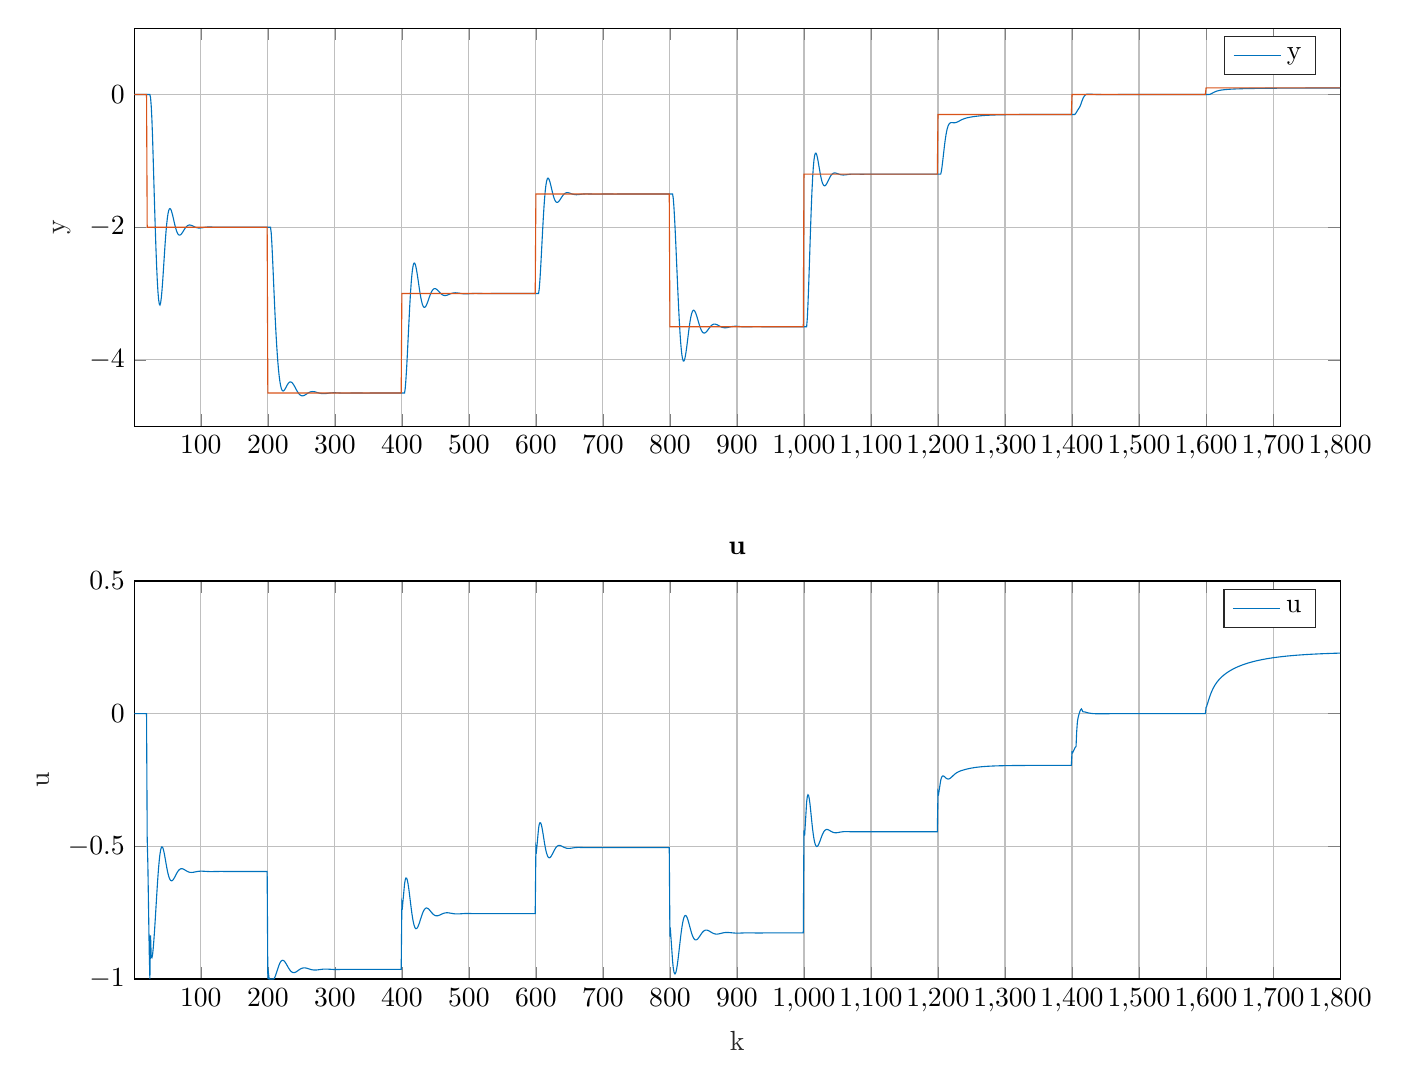
\begin{tikzpicture}

\begin{axis}[%
width=6.028in,
height=1.99in,
at={(1.011in,3.406in)},
scale only axis,
xmin=1,
xmax=1800,
ymin=-5,
ymax=1,
ylabel style={font=\color{white!15!black}},
ylabel={y},
axis background/.style={fill=white},
xmajorgrids,
ymajorgrids,
legend style={legend cell align=left, align=left, draw=white!15!black}
]
\addplot [color=mycolor1]
  table[row sep=crcr]{%
1	0\\
2	0\\
3	0\\
4	0\\
5	0\\
6	0\\
7	0\\
8	0\\
9	0\\
10	0\\
11	0\\
12	0\\
13	0\\
14	0\\
15	0\\
16	0\\
17	0\\
18	0\\
19	0\\
20	0\\
21	0\\
22	0\\
23	0\\
24	0\\
25	-0.046722\\
26	-0.17222\\
27	-0.37125\\
28	-0.64589\\
29	-0.98751\\
30	-1.3387\\
31	-1.6791\\
32	-2.0058\\
33	-2.3073\\
34	-2.5731\\
35	-2.7949\\
36	-2.9676\\
37	-3.0883\\
38	-3.1563\\
39	-3.1729\\
40	-3.1418\\
41	-3.0685\\
42	-2.9604\\
43	-2.8259\\
44	-2.6744\\
45	-2.5154\\
46	-2.3576\\
47	-2.2087\\
48	-2.0748\\
49	-1.9603\\
50	-1.8678\\
51	-1.7982\\
52	-1.7512\\
53	-1.7254\\
54	-1.7186\\
55	-1.7279\\
56	-1.7505\\
57	-1.7831\\
58	-1.8227\\
59	-1.8662\\
60	-1.911\\
61	-1.9547\\
62	-1.9955\\
63	-2.0317\\
64	-2.0622\\
65	-2.0864\\
66	-2.1039\\
67	-2.1146\\
68	-2.1191\\
69	-2.1178\\
70	-2.1116\\
71	-2.1014\\
72	-2.0881\\
73	-2.0729\\
74	-2.0566\\
75	-2.0402\\
76	-2.0245\\
77	-2.01\\
78	-1.9973\\
79	-1.9866\\
80	-1.9783\\
81	-1.9724\\
82	-1.9687\\
83	-1.9671\\
84	-1.9674\\
85	-1.9693\\
86	-1.9725\\
87	-1.9766\\
88	-1.9813\\
89	-1.9863\\
90	-1.9913\\
91	-1.9961\\
92	-2.0004\\
93	-2.0041\\
94	-2.0072\\
95	-2.0095\\
96	-2.0111\\
97	-2.012\\
98	-2.0122\\
99	-2.0118\\
100	-2.0109\\
101	-2.0097\\
102	-2.0082\\
103	-2.0065\\
104	-2.0048\\
105	-2.0031\\
106	-2.0015\\
107	-2.0001\\
108	-1.9989\\
109	-1.9979\\
110	-1.9971\\
111	-1.9966\\
112	-1.9964\\
113	-1.9963\\
114	-1.9965\\
115	-1.9968\\
116	-1.9972\\
117	-1.9976\\
118	-1.9982\\
119	-1.9987\\
120	-1.9993\\
121	-1.9998\\
122	-2.0002\\
123	-2.0006\\
124	-2.0009\\
125	-2.0011\\
126	-2.0012\\
127	-2.0013\\
128	-2.0013\\
129	-2.0012\\
130	-2.0011\\
131	-2.0009\\
132	-2.0008\\
133	-2.0006\\
134	-2.0004\\
135	-2.0002\\
136	-2.0001\\
137	-1.9999\\
138	-1.9998\\
139	-1.9997\\
140	-1.9997\\
141	-1.9996\\
142	-1.9996\\
143	-1.9996\\
144	-1.9996\\
145	-1.9997\\
146	-1.9997\\
147	-1.9998\\
148	-1.9998\\
149	-1.9999\\
150	-1.9999\\
151	-2\\
152	-2\\
153	-2.0001\\
154	-2.0001\\
155	-2.0001\\
156	-2.0001\\
157	-2.0001\\
158	-2.0001\\
159	-2.0001\\
160	-2.0001\\
161	-2.0001\\
162	-2.0001\\
163	-2.0001\\
164	-2\\
165	-2\\
166	-2\\
167	-2\\
168	-2\\
169	-2\\
170	-2\\
171	-2\\
172	-2\\
173	-2\\
174	-2\\
175	-2\\
176	-2\\
177	-2\\
178	-2\\
179	-2\\
180	-2\\
181	-2\\
182	-2\\
183	-2\\
184	-2\\
185	-2\\
186	-2\\
187	-2\\
188	-2\\
189	-2\\
190	-2\\
191	-2\\
192	-2\\
193	-2\\
194	-2\\
195	-2\\
196	-2\\
197	-2\\
198	-2\\
199	-2\\
200	-2\\
201	-2\\
202	-2\\
203	-2\\
204	-2\\
205	-2.0801\\
206	-2.2427\\
207	-2.4526\\
208	-2.6856\\
209	-2.9234\\
210	-3.1541\\
211	-3.3704\\
212	-3.5682\\
213	-3.7459\\
214	-3.903\\
215	-4.0393\\
216	-4.155\\
217	-4.2505\\
218	-4.3267\\
219	-4.3847\\
220	-4.426\\
221	-4.4525\\
222	-4.4661\\
223	-4.4689\\
224	-4.4632\\
225	-4.451\\
226	-4.4346\\
227	-4.4158\\
228	-4.3963\\
229	-4.3778\\
230	-4.3614\\
231	-4.3482\\
232	-4.3387\\
233	-4.3334\\
234	-4.3325\\
235	-4.3358\\
236	-4.3431\\
237	-4.354\\
238	-4.3678\\
239	-4.3839\\
240	-4.4017\\
241	-4.4205\\
242	-4.4394\\
243	-4.458\\
244	-4.4756\\
245	-4.4917\\
246	-4.5059\\
247	-4.5179\\
248	-4.5275\\
249	-4.5347\\
250	-4.5394\\
251	-4.5418\\
252	-4.5419\\
253	-4.5402\\
254	-4.5368\\
255	-4.532\\
256	-4.5263\\
257	-4.52\\
258	-4.5133\\
259	-4.5066\\
260	-4.5002\\
261	-4.4944\\
262	-4.4892\\
263	-4.4849\\
264	-4.4816\\
265	-4.4792\\
266	-4.4779\\
267	-4.4775\\
268	-4.478\\
269	-4.4793\\
270	-4.4812\\
271	-4.4836\\
272	-4.4865\\
273	-4.4895\\
274	-4.4927\\
275	-4.4958\\
276	-4.4988\\
277	-4.5015\\
278	-4.5038\\
279	-4.5058\\
280	-4.5073\\
281	-4.5084\\
282	-4.5091\\
283	-4.5093\\
284	-4.5091\\
285	-4.5086\\
286	-4.5078\\
287	-4.5067\\
288	-4.5055\\
289	-4.5042\\
290	-4.5028\\
291	-4.5015\\
292	-4.5002\\
293	-4.4991\\
294	-4.4981\\
295	-4.4973\\
296	-4.4966\\
297	-4.4962\\
298	-4.4959\\
299	-4.4958\\
300	-4.496\\
301	-4.4962\\
302	-4.4966\\
303	-4.4971\\
304	-4.4976\\
305	-4.4982\\
306	-4.4988\\
307	-4.4994\\
308	-4.4999\\
309	-4.5004\\
310	-4.5009\\
311	-4.5012\\
312	-4.5015\\
313	-4.5017\\
314	-4.5018\\
315	-4.5018\\
316	-4.5018\\
317	-4.5016\\
318	-4.5015\\
319	-4.5013\\
320	-4.501\\
321	-4.5008\\
322	-4.5005\\
323	-4.5003\\
324	-4.5\\
325	-4.4998\\
326	-4.4996\\
327	-4.4995\\
328	-4.4993\\
329	-4.4993\\
330	-4.4992\\
331	-4.4992\\
332	-4.4992\\
333	-4.4993\\
334	-4.4994\\
335	-4.4995\\
336	-4.4996\\
337	-4.4997\\
338	-4.4998\\
339	-4.4999\\
340	-4.5\\
341	-4.5001\\
342	-4.5002\\
343	-4.5002\\
344	-4.5003\\
345	-4.5003\\
346	-4.5003\\
347	-4.5003\\
348	-4.5003\\
349	-4.5003\\
350	-4.5003\\
351	-4.5002\\
352	-4.5002\\
353	-4.5001\\
354	-4.5001\\
355	-4.5\\
356	-4.5\\
357	-4.5\\
358	-4.4999\\
359	-4.4999\\
360	-4.4999\\
361	-4.4999\\
362	-4.4998\\
363	-4.4998\\
364	-4.4999\\
365	-4.4999\\
366	-4.4999\\
367	-4.4999\\
368	-4.4999\\
369	-4.4999\\
370	-4.5\\
371	-4.5\\
372	-4.5\\
373	-4.5\\
374	-4.5\\
375	-4.5\\
376	-4.5001\\
377	-4.5001\\
378	-4.5001\\
379	-4.5001\\
380	-4.5001\\
381	-4.5001\\
382	-4.5001\\
383	-4.5\\
384	-4.5\\
385	-4.5\\
386	-4.5\\
387	-4.5\\
388	-4.5\\
389	-4.5\\
390	-4.5\\
391	-4.5\\
392	-4.5\\
393	-4.5\\
394	-4.5\\
395	-4.5\\
396	-4.5\\
397	-4.5\\
398	-4.5\\
399	-4.5\\
400	-4.5\\
401	-4.5\\
402	-4.5\\
403	-4.5\\
404	-4.5\\
405	-4.4319\\
406	-4.3057\\
407	-4.143\\
408	-3.9553\\
409	-3.7516\\
410	-3.5418\\
411	-3.3365\\
412	-3.1448\\
413	-2.9739\\
414	-2.8288\\
415	-2.7127\\
416	-2.6269\\
417	-2.5708\\
418	-2.5429\\
419	-2.5405\\
420	-2.5601\\
421	-2.598\\
422	-2.65\\
423	-2.7121\\
424	-2.7804\\
425	-2.851\\
426	-2.9208\\
427	-2.9868\\
428	-3.0467\\
429	-3.0985\\
430	-3.1409\\
431	-3.1731\\
432	-3.1949\\
433	-3.2063\\
434	-3.2081\\
435	-3.2012\\
436	-3.1867\\
437	-3.1662\\
438	-3.1412\\
439	-3.1133\\
440	-3.0839\\
441	-3.0545\\
442	-3.0265\\
443	-3.0007\\
444	-2.9781\\
445	-2.9593\\
446	-2.9446\\
447	-2.9341\\
448	-2.9279\\
449	-2.9256\\
450	-2.9268\\
451	-2.9311\\
452	-2.938\\
453	-2.9468\\
454	-2.9569\\
455	-2.9677\\
456	-2.9786\\
457	-2.9893\\
458	-2.9992\\
459	-3.008\\
460	-3.0155\\
461	-3.0215\\
462	-3.0258\\
463	-3.0286\\
464	-3.0298\\
465	-3.0297\\
466	-3.0282\\
467	-3.0258\\
468	-3.0225\\
469	-3.0187\\
470	-3.0145\\
471	-3.0102\\
472	-3.0059\\
473	-3.0019\\
474	-2.9983\\
475	-2.9952\\
476	-2.9927\\
477	-2.9908\\
478	-2.9895\\
479	-2.9888\\
480	-2.9887\\
481	-2.9891\\
482	-2.9899\\
483	-2.9911\\
484	-2.9925\\
485	-2.994\\
486	-2.9957\\
487	-2.9973\\
488	-2.9989\\
489	-3.0003\\
490	-3.0016\\
491	-3.0026\\
492	-3.0034\\
493	-3.004\\
494	-3.0043\\
495	-3.0044\\
496	-3.0043\\
497	-3.004\\
498	-3.0036\\
499	-3.0031\\
500	-3.0025\\
501	-3.0019\\
502	-3.0012\\
503	-3.0006\\
504	-3.0001\\
505	-2.9996\\
506	-2.9991\\
507	-2.9988\\
508	-2.9985\\
509	-2.9984\\
510	-2.9983\\
511	-2.9983\\
512	-2.9984\\
513	-2.9986\\
514	-2.9987\\
515	-2.999\\
516	-2.9992\\
517	-2.9994\\
518	-2.9997\\
519	-2.9999\\
520	-3.0001\\
521	-3.0003\\
522	-3.0004\\
523	-3.0005\\
524	-3.0006\\
525	-3.0006\\
526	-3.0007\\
527	-3.0006\\
528	-3.0006\\
529	-3.0005\\
530	-3.0004\\
531	-3.0003\\
532	-3.0002\\
533	-3.0001\\
534	-3.0001\\
535	-3\\
536	-2.9999\\
537	-2.9998\\
538	-2.9998\\
539	-2.9998\\
540	-2.9998\\
541	-2.9997\\
542	-2.9998\\
543	-2.9998\\
544	-2.9998\\
545	-2.9998\\
546	-2.9999\\
547	-2.9999\\
548	-2.9999\\
549	-3\\
550	-3\\
551	-3\\
552	-3.0001\\
553	-3.0001\\
554	-3.0001\\
555	-3.0001\\
556	-3.0001\\
557	-3.0001\\
558	-3.0001\\
559	-3.0001\\
560	-3.0001\\
561	-3.0001\\
562	-3\\
563	-3\\
564	-3\\
565	-3\\
566	-3\\
567	-3\\
568	-3\\
569	-3\\
570	-3\\
571	-3\\
572	-3\\
573	-3\\
574	-3\\
575	-3\\
576	-3\\
577	-3\\
578	-3\\
579	-3\\
580	-3\\
581	-3\\
582	-3\\
583	-3\\
584	-3\\
585	-3\\
586	-3\\
587	-3\\
588	-3\\
589	-3\\
590	-3\\
591	-3\\
592	-3\\
593	-3\\
594	-3\\
595	-3\\
596	-3\\
597	-3\\
598	-3\\
599	-3\\
600	-3\\
601	-3\\
602	-3\\
603	-3\\
604	-3\\
605	-2.9262\\
606	-2.7955\\
607	-2.631\\
608	-2.4459\\
609	-2.2501\\
610	-2.0544\\
611	-1.8697\\
612	-1.704\\
613	-1.5627\\
614	-1.4488\\
615	-1.363\\
616	-1.3044\\
617	-1.2709\\
618	-1.2593\\
619	-1.266\\
620	-1.2872\\
621	-1.3192\\
622	-1.3582\\
623	-1.401\\
624	-1.4446\\
625	-1.4866\\
626	-1.5249\\
627	-1.558\\
628	-1.5849\\
629	-1.6051\\
630	-1.6185\\
631	-1.6252\\
632	-1.6259\\
633	-1.6214\\
634	-1.6125\\
635	-1.6003\\
636	-1.5858\\
637	-1.5701\\
638	-1.5541\\
639	-1.5386\\
640	-1.5242\\
641	-1.5115\\
642	-1.5007\\
643	-1.4921\\
644	-1.4858\\
645	-1.4815\\
646	-1.4792\\
647	-1.4787\\
648	-1.4796\\
649	-1.4816\\
650	-1.4845\\
651	-1.488\\
652	-1.4917\\
653	-1.4954\\
654	-1.4989\\
655	-1.502\\
656	-1.5047\\
657	-1.5069\\
658	-1.5084\\
659	-1.5094\\
660	-1.5099\\
661	-1.5098\\
662	-1.5094\\
663	-1.5086\\
664	-1.5076\\
665	-1.5064\\
666	-1.5051\\
667	-1.5039\\
668	-1.5026\\
669	-1.5015\\
670	-1.5005\\
671	-1.4997\\
672	-1.4991\\
673	-1.4986\\
674	-1.4983\\
675	-1.4982\\
676	-1.4982\\
677	-1.4983\\
678	-1.4985\\
679	-1.4987\\
680	-1.499\\
681	-1.4993\\
682	-1.4996\\
683	-1.4999\\
684	-1.5002\\
685	-1.5004\\
686	-1.5006\\
687	-1.5007\\
688	-1.5007\\
689	-1.5008\\
690	-1.5008\\
691	-1.5007\\
692	-1.5007\\
693	-1.5006\\
694	-1.5005\\
695	-1.5004\\
696	-1.5003\\
697	-1.5002\\
698	-1.5001\\
699	-1.5\\
700	-1.5\\
701	-1.4999\\
702	-1.4999\\
703	-1.4999\\
704	-1.4998\\
705	-1.4998\\
706	-1.4999\\
707	-1.4999\\
708	-1.4999\\
709	-1.4999\\
710	-1.4999\\
711	-1.5\\
712	-1.5\\
713	-1.5\\
714	-1.5\\
715	-1.5\\
716	-1.5001\\
717	-1.5001\\
718	-1.5001\\
719	-1.5001\\
720	-1.5001\\
721	-1.5001\\
722	-1.5\\
723	-1.5\\
724	-1.5\\
725	-1.5\\
726	-1.5\\
727	-1.5\\
728	-1.5\\
729	-1.5\\
730	-1.5\\
731	-1.5\\
732	-1.5\\
733	-1.5\\
734	-1.5\\
735	-1.5\\
736	-1.5\\
737	-1.5\\
738	-1.5\\
739	-1.5\\
740	-1.5\\
741	-1.5\\
742	-1.5\\
743	-1.5\\
744	-1.5\\
745	-1.5\\
746	-1.5\\
747	-1.5\\
748	-1.5\\
749	-1.5\\
750	-1.5\\
751	-1.5\\
752	-1.5\\
753	-1.5\\
754	-1.5\\
755	-1.5\\
756	-1.5\\
757	-1.5\\
758	-1.5\\
759	-1.5\\
760	-1.5\\
761	-1.5\\
762	-1.5\\
763	-1.5\\
764	-1.5\\
765	-1.5\\
766	-1.5\\
767	-1.5\\
768	-1.5\\
769	-1.5\\
770	-1.5\\
771	-1.5\\
772	-1.5\\
773	-1.5\\
774	-1.5\\
775	-1.5\\
776	-1.5\\
777	-1.5\\
778	-1.5\\
779	-1.5\\
780	-1.5\\
781	-1.5\\
782	-1.5\\
783	-1.5\\
784	-1.5\\
785	-1.5\\
786	-1.5\\
787	-1.5\\
788	-1.5\\
789	-1.5\\
790	-1.5\\
791	-1.5\\
792	-1.5\\
793	-1.5\\
794	-1.5\\
795	-1.5\\
796	-1.5\\
797	-1.5\\
798	-1.5\\
799	-1.5\\
800	-1.5\\
801	-1.5\\
802	-1.5\\
803	-1.5\\
804	-1.5\\
805	-1.567\\
806	-1.7013\\
807	-1.877\\
808	-2.0809\\
809	-2.3039\\
810	-2.5375\\
811	-2.7728\\
812	-3.0019\\
813	-3.2178\\
814	-3.4145\\
815	-3.5876\\
816	-3.7335\\
817	-3.8499\\
818	-3.9358\\
819	-3.9911\\
820	-4.0172\\
821	-4.0161\\
822	-3.9909\\
823	-3.9454\\
824	-3.8839\\
825	-3.8108\\
826	-3.7307\\
827	-3.6481\\
828	-3.5669\\
829	-3.4908\\
830	-3.4227\\
831	-3.3645\\
832	-3.3179\\
833	-3.2836\\
834	-3.2617\\
835	-3.2518\\
836	-3.2529\\
837	-3.2638\\
838	-3.283\\
839	-3.3087\\
840	-3.3393\\
841	-3.3729\\
842	-3.4078\\
843	-3.4426\\
844	-3.4758\\
845	-3.5062\\
846	-3.533\\
847	-3.5554\\
848	-3.573\\
849	-3.5856\\
850	-3.5932\\
851	-3.596\\
852	-3.5945\\
853	-3.5892\\
854	-3.5807\\
855	-3.5697\\
856	-3.5569\\
857	-3.5432\\
858	-3.5291\\
859	-3.5153\\
860	-3.5024\\
861	-3.4908\\
862	-3.4808\\
863	-3.4727\\
864	-3.4666\\
865	-3.4626\\
866	-3.4605\\
867	-3.4604\\
868	-3.4619\\
869	-3.4648\\
870	-3.4688\\
871	-3.4737\\
872	-3.4792\\
873	-3.4849\\
874	-3.4906\\
875	-3.4961\\
876	-3.5011\\
877	-3.5056\\
878	-3.5093\\
879	-3.5122\\
880	-3.5143\\
881	-3.5156\\
882	-3.5161\\
883	-3.5159\\
884	-3.515\\
885	-3.5136\\
886	-3.5118\\
887	-3.5096\\
888	-3.5074\\
889	-3.505\\
890	-3.5027\\
891	-3.5006\\
892	-3.4986\\
893	-3.497\\
894	-3.4956\\
895	-3.4946\\
896	-3.4939\\
897	-3.4935\\
898	-3.4935\\
899	-3.4937\\
900	-3.4941\\
901	-3.4948\\
902	-3.4956\\
903	-3.4965\\
904	-3.4974\\
905	-3.4984\\
906	-3.4993\\
907	-3.5001\\
908	-3.5009\\
909	-3.5015\\
910	-3.502\\
911	-3.5024\\
912	-3.5026\\
913	-3.5027\\
914	-3.5026\\
915	-3.5025\\
916	-3.5023\\
917	-3.502\\
918	-3.5016\\
919	-3.5012\\
920	-3.5009\\
921	-3.5005\\
922	-3.5001\\
923	-3.4998\\
924	-3.4995\\
925	-3.4993\\
926	-3.4991\\
927	-3.499\\
928	-3.4989\\
929	-3.4989\\
930	-3.4989\\
931	-3.499\\
932	-3.4991\\
933	-3.4993\\
934	-3.4994\\
935	-3.4996\\
936	-3.4997\\
937	-3.4999\\
938	-3.5\\
939	-3.5001\\
940	-3.5002\\
941	-3.5003\\
942	-3.5004\\
943	-3.5004\\
944	-3.5004\\
945	-3.5004\\
946	-3.5004\\
947	-3.5004\\
948	-3.5003\\
949	-3.5003\\
950	-3.5002\\
951	-3.5001\\
952	-3.5001\\
953	-3.5\\
954	-3.5\\
955	-3.4999\\
956	-3.4999\\
957	-3.4999\\
958	-3.4998\\
959	-3.4998\\
960	-3.4998\\
961	-3.4998\\
962	-3.4998\\
963	-3.4999\\
964	-3.4999\\
965	-3.4999\\
966	-3.4999\\
967	-3.5\\
968	-3.5\\
969	-3.5\\
970	-3.5\\
971	-3.5\\
972	-3.5001\\
973	-3.5001\\
974	-3.5001\\
975	-3.5001\\
976	-3.5001\\
977	-3.5001\\
978	-3.5001\\
979	-3.5001\\
980	-3.5\\
981	-3.5\\
982	-3.5\\
983	-3.5\\
984	-3.5\\
985	-3.5\\
986	-3.5\\
987	-3.5\\
988	-3.5\\
989	-3.5\\
990	-3.5\\
991	-3.5\\
992	-3.5\\
993	-3.5\\
994	-3.5\\
995	-3.5\\
996	-3.5\\
997	-3.5\\
998	-3.5\\
999	-3.5\\
1000	-3.5\\
1001	-3.5\\
1002	-3.5\\
1003	-3.5\\
1004	-3.5\\
1005	-3.3746\\
1006	-3.1592\\
1007	-2.8907\\
1008	-2.5911\\
1009	-2.2772\\
1010	-1.9699\\
1011	-1.6876\\
1012	-1.4432\\
1013	-1.2434\\
1014	-1.0904\\
1015	-0.98243\\
1016	-0.91576\\
1017	-0.88498\\
1018	-0.88403\\
1019	-0.90662\\
1020	-0.94665\\
1021	-0.9984\\
1022	-1.0567\\
1023	-1.1171\\
1024	-1.1757\\
1025	-1.2296\\
1026	-1.2766\\
1027	-1.315\\
1028	-1.344\\
1029	-1.3635\\
1030	-1.3737\\
1031	-1.3755\\
1032	-1.3699\\
1033	-1.3582\\
1034	-1.3421\\
1035	-1.3229\\
1036	-1.3021\\
1037	-1.2809\\
1038	-1.2605\\
1039	-1.2416\\
1040	-1.225\\
1041	-1.211\\
1042	-1.1999\\
1043	-1.1916\\
1044	-1.1861\\
1045	-1.183\\
1046	-1.182\\
1047	-1.1828\\
1048	-1.1849\\
1049	-1.1879\\
1050	-1.1915\\
1051	-1.1954\\
1052	-1.1992\\
1053	-1.2028\\
1054	-1.2059\\
1055	-1.2084\\
1056	-1.2103\\
1057	-1.2116\\
1058	-1.2123\\
1059	-1.2124\\
1060	-1.212\\
1061	-1.2112\\
1062	-1.2102\\
1063	-1.2089\\
1064	-1.2075\\
1065	-1.2061\\
1066	-1.2047\\
1067	-1.2035\\
1068	-1.2023\\
1069	-1.2014\\
1070	-1.2006\\
1071	-1.2\\
1072	-1.1996\\
1073	-1.1993\\
1074	-1.1992\\
1075	-1.1992\\
1076	-1.1993\\
1077	-1.1994\\
1078	-1.1996\\
1079	-1.1999\\
1080	-1.2001\\
1081	-1.2003\\
1082	-1.2005\\
1083	-1.2006\\
1084	-1.2008\\
1085	-1.2008\\
1086	-1.2009\\
1087	-1.2009\\
1088	-1.2009\\
1089	-1.2008\\
1090	-1.2007\\
1091	-1.2007\\
1092	-1.2006\\
1093	-1.2005\\
1094	-1.2004\\
1095	-1.2003\\
1096	-1.2002\\
1097	-1.2001\\
1098	-1.2001\\
1099	-1.2\\
1100	-1.2\\
1101	-1.2\\
1102	-1.2\\
1103	-1.2\\
1104	-1.2\\
1105	-1.2\\
1106	-1.2\\
1107	-1.2\\
1108	-1.2\\
1109	-1.2\\
1110	-1.2\\
1111	-1.2001\\
1112	-1.2001\\
1113	-1.2001\\
1114	-1.2001\\
1115	-1.2001\\
1116	-1.2001\\
1117	-1.2001\\
1118	-1.2001\\
1119	-1.2\\
1120	-1.2\\
1121	-1.2\\
1122	-1.2\\
1123	-1.2\\
1124	-1.2\\
1125	-1.2\\
1126	-1.2\\
1127	-1.2\\
1128	-1.2\\
1129	-1.2\\
1130	-1.2\\
1131	-1.2\\
1132	-1.2\\
1133	-1.2\\
1134	-1.2\\
1135	-1.2\\
1136	-1.2\\
1137	-1.2\\
1138	-1.2\\
1139	-1.2\\
1140	-1.2\\
1141	-1.2\\
1142	-1.2\\
1143	-1.2\\
1144	-1.2\\
1145	-1.2\\
1146	-1.2\\
1147	-1.2\\
1148	-1.2\\
1149	-1.2\\
1150	-1.2\\
1151	-1.2\\
1152	-1.2\\
1153	-1.2\\
1154	-1.2\\
1155	-1.2\\
1156	-1.2\\
1157	-1.2\\
1158	-1.2\\
1159	-1.2\\
1160	-1.2\\
1161	-1.2\\
1162	-1.2\\
1163	-1.2\\
1164	-1.2\\
1165	-1.2\\
1166	-1.2\\
1167	-1.2\\
1168	-1.2\\
1169	-1.2\\
1170	-1.2\\
1171	-1.2\\
1172	-1.2\\
1173	-1.2\\
1174	-1.2\\
1175	-1.2\\
1176	-1.2\\
1177	-1.2\\
1178	-1.2\\
1179	-1.2\\
1180	-1.2\\
1181	-1.2\\
1182	-1.2\\
1183	-1.2\\
1184	-1.2\\
1185	-1.2\\
1186	-1.2\\
1187	-1.2\\
1188	-1.2\\
1189	-1.2\\
1190	-1.2\\
1191	-1.2\\
1192	-1.2\\
1193	-1.2\\
1194	-1.2\\
1195	-1.2\\
1196	-1.2\\
1197	-1.2\\
1198	-1.2\\
1199	-1.2\\
1200	-1.2\\
1201	-1.2\\
1202	-1.2\\
1203	-1.2\\
1204	-1.2\\
1205	-1.1595\\
1206	-1.0904\\
1207	-1.0075\\
1208	-0.91874\\
1209	-0.82958\\
1210	-0.7449\\
1211	-0.66863\\
1212	-0.60311\\
1213	-0.54926\\
1214	-0.50692\\
1215	-0.4752\\
1216	-0.45274\\
1217	-0.43794\\
1218	-0.42911\\
1219	-0.42465\\
1220	-0.42312\\
1221	-0.42329\\
1222	-0.42418\\
1223	-0.42504\\
1224	-0.42536\\
1225	-0.42481\\
1226	-0.42326\\
1227	-0.4207\\
1228	-0.41721\\
1229	-0.41295\\
1230	-0.40811\\
1231	-0.40289\\
1232	-0.39746\\
1233	-0.392\\
1234	-0.38665\\
1235	-0.38152\\
1236	-0.37667\\
1237	-0.37216\\
1238	-0.36799\\
1239	-0.36418\\
1240	-0.3607\\
1241	-0.35754\\
1242	-0.35465\\
1243	-0.352\\
1244	-0.34956\\
1245	-0.34729\\
1246	-0.34517\\
1247	-0.34318\\
1248	-0.34129\\
1249	-0.33949\\
1250	-0.33777\\
1251	-0.33611\\
1252	-0.33452\\
1253	-0.33299\\
1254	-0.33152\\
1255	-0.33011\\
1256	-0.32875\\
1257	-0.32745\\
1258	-0.3262\\
1259	-0.32501\\
1260	-0.32388\\
1261	-0.32279\\
1262	-0.32176\\
1263	-0.32077\\
1264	-0.31984\\
1265	-0.31895\\
1266	-0.3181\\
1267	-0.31729\\
1268	-0.31651\\
1269	-0.31578\\
1270	-0.31508\\
1271	-0.31441\\
1272	-0.31377\\
1273	-0.31316\\
1274	-0.31258\\
1275	-0.31203\\
1276	-0.3115\\
1277	-0.31099\\
1278	-0.31051\\
1279	-0.31005\\
1280	-0.3096\\
1281	-0.30918\\
1282	-0.30878\\
1283	-0.30839\\
1284	-0.30802\\
1285	-0.30767\\
1286	-0.30733\\
1287	-0.30701\\
1288	-0.30671\\
1289	-0.30641\\
1290	-0.30613\\
1291	-0.30586\\
1292	-0.30561\\
1293	-0.30536\\
1294	-0.30513\\
1295	-0.3049\\
1296	-0.30469\\
1297	-0.30448\\
1298	-0.30429\\
1299	-0.3041\\
1300	-0.30392\\
1301	-0.30375\\
1302	-0.30359\\
1303	-0.30343\\
1304	-0.30328\\
1305	-0.30314\\
1306	-0.303\\
1307	-0.30287\\
1308	-0.30275\\
1309	-0.30263\\
1310	-0.30251\\
1311	-0.3024\\
1312	-0.3023\\
1313	-0.3022\\
1314	-0.3021\\
1315	-0.30201\\
1316	-0.30192\\
1317	-0.30184\\
1318	-0.30176\\
1319	-0.30168\\
1320	-0.30161\\
1321	-0.30154\\
1322	-0.30147\\
1323	-0.30141\\
1324	-0.30135\\
1325	-0.30129\\
1326	-0.30123\\
1327	-0.30118\\
1328	-0.30113\\
1329	-0.30108\\
1330	-0.30103\\
1331	-0.30099\\
1332	-0.30095\\
1333	-0.3009\\
1334	-0.30087\\
1335	-0.30083\\
1336	-0.30079\\
1337	-0.30076\\
1338	-0.30072\\
1339	-0.30069\\
1340	-0.30066\\
1341	-0.30063\\
1342	-0.30061\\
1343	-0.30058\\
1344	-0.30056\\
1345	-0.30053\\
1346	-0.30051\\
1347	-0.30049\\
1348	-0.30046\\
1349	-0.30044\\
1350	-0.30043\\
1351	-0.30041\\
1352	-0.30039\\
1353	-0.30037\\
1354	-0.30036\\
1355	-0.30034\\
1356	-0.30033\\
1357	-0.30031\\
1358	-0.3003\\
1359	-0.30029\\
1360	-0.30027\\
1361	-0.30026\\
1362	-0.30025\\
1363	-0.30024\\
1364	-0.30023\\
1365	-0.30022\\
1366	-0.30021\\
1367	-0.3002\\
1368	-0.30019\\
1369	-0.30018\\
1370	-0.30018\\
1371	-0.30017\\
1372	-0.30016\\
1373	-0.30015\\
1374	-0.30015\\
1375	-0.30014\\
1376	-0.30013\\
1377	-0.30013\\
1378	-0.30012\\
1379	-0.30012\\
1380	-0.30011\\
1381	-0.30011\\
1382	-0.3001\\
1383	-0.3001\\
1384	-0.30009\\
1385	-0.30009\\
1386	-0.30009\\
1387	-0.30008\\
1388	-0.30008\\
1389	-0.30008\\
1390	-0.30007\\
1391	-0.30007\\
1392	-0.30007\\
1393	-0.30006\\
1394	-0.30006\\
1395	-0.30006\\
1396	-0.30006\\
1397	-0.30005\\
1398	-0.30005\\
1399	-0.30005\\
1400	-0.30005\\
1401	-0.30004\\
1402	-0.30004\\
1403	-0.30004\\
1404	-0.30004\\
1405	-0.2917\\
1406	-0.27707\\
1407	-0.26021\\
1408	-0.24291\\
1409	-0.22617\\
1410	-0.21067\\
1411	-0.19685\\
1412	-0.17785\\
1413	-0.15151\\
1414	-0.12184\\
1415	-0.093042\\
1416	-0.067422\\
1417	-0.045827\\
1418	-0.028371\\
1419	-0.014777\\
1420	-0.0048728\\
1421	0.0014373\\
1422	0.0048604\\
1423	0.00648\\
1424	0.0070753\\
1425	0.0070758\\
1426	0.0067294\\
1427	0.0061924\\
1428	0.005566\\
1429	0.0049132\\
1430	0.0042715\\
1431	0.0036628\\
1432	0.0030994\\
1433	0.0025874\\
1434	0.0021286\\
1435	0.0017228\\
1436	0.0013677\\
1437	0.0010605\\
1438	0.00079754\\
1439	0.00057494\\
1440	0.00038876\\
1441	0.00023511\\
1442	0.00011021\\
1443	1.0491e-05\\
1444	-6.7409e-05\\
1445	-0.00012658\\
1446	-0.00016985\\
1447	-0.00019977\\
1448	-0.00021863\\
1449	-0.00022845\\
1450	-0.00023101\\
1451	-0.00022787\\
1452	-0.00022036\\
1453	-0.0002096\\
1454	-0.00019657\\
1455	-0.00018204\\
1456	-0.00016668\\
1457	-0.00015101\\
1458	-0.00013545\\
1459	-0.00012032\\
1460	-0.00010586\\
1461	-9.2254e-05\\
1462	-7.9605e-05\\
1463	-6.7987e-05\\
1464	-5.7429e-05\\
1465	-4.7931e-05\\
1466	-3.9471e-05\\
1467	-3.2006e-05\\
1468	-2.5483e-05\\
1469	-1.9837e-05\\
1470	-1.5001e-05\\
1471	-1.0902e-05\\
1472	-7.4679e-06\\
1473	-4.6285e-06\\
1474	-2.315e-06\\
1475	-4.6227e-07\\
1476	9.9047e-07\\
1477	2.0995e-06\\
1478	2.9163e-06\\
1479	3.4875e-06\\
1480	3.8546e-06\\
1481	4.0548e-06\\
1482	4.1205e-06\\
1483	4.0801e-06\\
1484	3.958e-06\\
1485	3.7749e-06\\
1486	3.5485e-06\\
1487	3.2934e-06\\
1488	3.0215e-06\\
1489	2.7427e-06\\
1490	2.4647e-06\\
1491	2.1934e-06\\
1492	1.9335e-06\\
1493	1.6882e-06\\
1494	1.4596e-06\\
1495	1.2492e-06\\
1496	1.0577e-06\\
1497	8.8504e-07\\
1498	7.3095e-07\\
1499	5.9474e-07\\
1500	4.7547e-07\\
1501	3.7204e-07\\
1502	2.8325e-07\\
1503	2.0782e-07\\
1504	1.4448e-07\\
1505	9.1946e-08\\
1506	4.9005e-08\\
1507	1.4483e-08\\
1508	-1.2716e-08\\
1509	-3.361e-08\\
1510	-4.9131e-08\\
1511	-6.0122e-08\\
1512	-6.7344e-08\\
1513	-7.147e-08\\
1514	-7.3093e-08\\
1515	-7.2733e-08\\
1516	-7.0836e-08\\
1517	-6.7784e-08\\
1518	-6.3902e-08\\
1519	-5.9459e-08\\
1520	-5.4678e-08\\
1521	-4.9741e-08\\
1522	-4.4792e-08\\
1523	-3.9942e-08\\
1524	-3.5279e-08\\
1525	-3.0865e-08\\
1526	-2.6742e-08\\
1527	-2.2937e-08\\
1528	-1.9465e-08\\
1529	-1.633e-08\\
1530	-1.3525e-08\\
1531	-1.1041e-08\\
1532	-8.862e-09\\
1533	-6.9683e-09\\
1534	-5.339e-09\\
1535	-3.9518e-09\\
1536	-2.784e-09\\
1537	-1.8129e-09\\
1538	-1.0165e-09\\
1539	-3.7391e-10\\
1540	1.3472e-10\\
1541	5.2774e-10\\
1542	8.22e-10\\
1543	1.0328e-09\\
1544	1.174e-09\\
1545	1.2579e-09\\
1546	1.2952e-09\\
1547	1.2954e-09\\
1548	1.2668e-09\\
1549	1.2164e-09\\
1550	1.1501e-09\\
1551	1.073e-09\\
1552	9.8904e-10\\
1553	9.0172e-10\\
1554	8.1368e-10\\
1555	7.2706e-10\\
1556	6.4346e-10\\
1557	5.6407e-10\\
1558	4.8972e-10\\
1559	4.2095e-10\\
1560	3.5805e-10\\
1561	3.0112e-10\\
1562	2.5011e-10\\
1563	2.0483e-10\\
1564	1.6503e-10\\
1565	1.3037e-10\\
1566	1.0049e-10\\
1567	7.4988e-11\\
1568	5.347e-11\\
1569	3.5528e-11\\
1570	2.0769e-11\\
1571	8.8164e-12\\
1572	-6.8526e-13\\
1573	-8.0677e-12\\
1574	-1.3636e-11\\
1575	-1.7669e-11\\
1576	-2.0415e-11\\
1577	-2.21e-11\\
1578	-2.2921e-11\\
1579	-2.305e-11\\
1580	-2.2638e-11\\
1581	-2.1815e-11\\
1582	-2.0689e-11\\
1583	-1.9352e-11\\
1584	-1.7882e-11\\
1585	-1.6339e-11\\
1586	-1.4775e-11\\
1587	-1.3229e-11\\
1588	-1.1731e-11\\
1589	-1.0304e-11\\
1590	-8.9643e-12\\
1591	-7.7219e-12\\
1592	-6.5829e-12\\
1593	-5.5498e-12\\
1594	-4.6221e-12\\
1595	-3.7972e-12\\
1596	-3.0705e-12\\
1597	-2.4364e-12\\
1598	-1.8886e-12\\
1599	-1.4202e-12\\
1600	-1.0239e-12\\
1601	-6.9257e-13\\
1602	-4.1924e-13\\
1603	-1.9711e-13\\
1604	-1.9789e-14\\
1605	0.0014818\\
1606	0.0049077\\
1607	0.00936\\
1608	0.014417\\
1609	0.019762\\
1610	0.025159\\
1611	0.030424\\
1612	0.035423\\
1613	0.040075\\
1614	0.044339\\
1615	0.048206\\
1616	0.051687\\
1617	0.054804\\
1618	0.05759\\
1619	0.060079\\
1620	0.062306\\
1621	0.064303\\
1622	0.0661\\
1623	0.067725\\
1624	0.069201\\
1625	0.070547\\
1626	0.071782\\
1627	0.07292\\
1628	0.073972\\
1629	0.07495\\
1630	0.075862\\
1631	0.076716\\
1632	0.077517\\
1633	0.07827\\
1634	0.078982\\
1635	0.079655\\
1636	0.080292\\
1637	0.080897\\
1638	0.081472\\
1639	0.08202\\
1640	0.082543\\
1641	0.083042\\
1642	0.083519\\
1643	0.083976\\
1644	0.084413\\
1645	0.084833\\
1646	0.085235\\
1647	0.085622\\
1648	0.085994\\
1649	0.086352\\
1650	0.086696\\
1651	0.087028\\
1652	0.087348\\
1653	0.087657\\
1654	0.087955\\
1655	0.088243\\
1656	0.088522\\
1657	0.088791\\
1658	0.089051\\
1659	0.089303\\
1660	0.089547\\
1661	0.089783\\
1662	0.090012\\
1663	0.090235\\
1664	0.09045\\
1665	0.090659\\
1666	0.090862\\
1667	0.091059\\
1668	0.091251\\
1669	0.091437\\
1670	0.091618\\
1671	0.091793\\
1672	0.091964\\
1673	0.092131\\
1674	0.092293\\
1675	0.09245\\
1676	0.092604\\
1677	0.092753\\
1678	0.092899\\
1679	0.093041\\
1680	0.093179\\
1681	0.093314\\
1682	0.093446\\
1683	0.093574\\
1684	0.093699\\
1685	0.093821\\
1686	0.09394\\
1687	0.094057\\
1688	0.09417\\
1689	0.094281\\
1690	0.094389\\
1691	0.094495\\
1692	0.094599\\
1693	0.0947\\
1694	0.094798\\
1695	0.094895\\
1696	0.094989\\
1697	0.095081\\
1698	0.095172\\
1699	0.09526\\
1700	0.095346\\
1701	0.095431\\
1702	0.095513\\
1703	0.095594\\
1704	0.095673\\
1705	0.095751\\
1706	0.095827\\
1707	0.095901\\
1708	0.095974\\
1709	0.096045\\
1710	0.096115\\
1711	0.096183\\
1712	0.09625\\
1713	0.096315\\
1714	0.09638\\
1715	0.096443\\
1716	0.096504\\
1717	0.096565\\
1718	0.096624\\
1719	0.096682\\
1720	0.096739\\
1721	0.096795\\
1722	0.09685\\
1723	0.096903\\
1724	0.096956\\
1725	0.097008\\
1726	0.097058\\
1727	0.097108\\
1728	0.097157\\
1729	0.097205\\
1730	0.097252\\
1731	0.097298\\
1732	0.097343\\
1733	0.097387\\
1734	0.097431\\
1735	0.097474\\
1736	0.097515\\
1737	0.097557\\
1738	0.097597\\
1739	0.097637\\
1740	0.097676\\
1741	0.097714\\
1742	0.097751\\
1743	0.097788\\
1744	0.097825\\
1745	0.09786\\
1746	0.097895\\
1747	0.097929\\
1748	0.097963\\
1749	0.097996\\
1750	0.098029\\
1751	0.098061\\
1752	0.098092\\
1753	0.098123\\
1754	0.098153\\
1755	0.098183\\
1756	0.098212\\
1757	0.098241\\
1758	0.098269\\
1759	0.098297\\
1760	0.098324\\
1761	0.098351\\
1762	0.098377\\
1763	0.098403\\
1764	0.098429\\
1765	0.098454\\
1766	0.098478\\
1767	0.098502\\
1768	0.098526\\
1769	0.09855\\
1770	0.098573\\
1771	0.098595\\
1772	0.098617\\
1773	0.098639\\
1774	0.098661\\
1775	0.098682\\
1776	0.098702\\
1777	0.098723\\
1778	0.098743\\
1779	0.098763\\
1780	0.098782\\
1781	0.098801\\
1782	0.09882\\
1783	0.098838\\
1784	0.098857\\
1785	0.098874\\
1786	0.098892\\
1787	0.098909\\
1788	0.098926\\
1789	0.098943\\
1790	0.098959\\
1791	0.098976\\
1792	0.098991\\
1793	0.099007\\
1794	0.099023\\
1795	0.099038\\
1796	0.099053\\
1797	0.099067\\
1798	0.099082\\
1799	0.099096\\
1800	0.09911\\
};
\addlegendentry{y}

\addplot [color=mycolor2, forget plot]
  table[row sep=crcr]{%
1	0\\
2	0\\
3	0\\
4	0\\
5	0\\
6	0\\
7	0\\
8	0\\
9	0\\
10	0\\
11	0\\
12	0\\
13	0\\
14	0\\
15	0\\
16	0\\
17	0\\
18	0\\
19	0\\
20	-2\\
21	-2\\
22	-2\\
23	-2\\
24	-2\\
25	-2\\
26	-2\\
27	-2\\
28	-2\\
29	-2\\
30	-2\\
31	-2\\
32	-2\\
33	-2\\
34	-2\\
35	-2\\
36	-2\\
37	-2\\
38	-2\\
39	-2\\
40	-2\\
41	-2\\
42	-2\\
43	-2\\
44	-2\\
45	-2\\
46	-2\\
47	-2\\
48	-2\\
49	-2\\
50	-2\\
51	-2\\
52	-2\\
53	-2\\
54	-2\\
55	-2\\
56	-2\\
57	-2\\
58	-2\\
59	-2\\
60	-2\\
61	-2\\
62	-2\\
63	-2\\
64	-2\\
65	-2\\
66	-2\\
67	-2\\
68	-2\\
69	-2\\
70	-2\\
71	-2\\
72	-2\\
73	-2\\
74	-2\\
75	-2\\
76	-2\\
77	-2\\
78	-2\\
79	-2\\
80	-2\\
81	-2\\
82	-2\\
83	-2\\
84	-2\\
85	-2\\
86	-2\\
87	-2\\
88	-2\\
89	-2\\
90	-2\\
91	-2\\
92	-2\\
93	-2\\
94	-2\\
95	-2\\
96	-2\\
97	-2\\
98	-2\\
99	-2\\
100	-2\\
101	-2\\
102	-2\\
103	-2\\
104	-2\\
105	-2\\
106	-2\\
107	-2\\
108	-2\\
109	-2\\
110	-2\\
111	-2\\
112	-2\\
113	-2\\
114	-2\\
115	-2\\
116	-2\\
117	-2\\
118	-2\\
119	-2\\
120	-2\\
121	-2\\
122	-2\\
123	-2\\
124	-2\\
125	-2\\
126	-2\\
127	-2\\
128	-2\\
129	-2\\
130	-2\\
131	-2\\
132	-2\\
133	-2\\
134	-2\\
135	-2\\
136	-2\\
137	-2\\
138	-2\\
139	-2\\
140	-2\\
141	-2\\
142	-2\\
143	-2\\
144	-2\\
145	-2\\
146	-2\\
147	-2\\
148	-2\\
149	-2\\
150	-2\\
151	-2\\
152	-2\\
153	-2\\
154	-2\\
155	-2\\
156	-2\\
157	-2\\
158	-2\\
159	-2\\
160	-2\\
161	-2\\
162	-2\\
163	-2\\
164	-2\\
165	-2\\
166	-2\\
167	-2\\
168	-2\\
169	-2\\
170	-2\\
171	-2\\
172	-2\\
173	-2\\
174	-2\\
175	-2\\
176	-2\\
177	-2\\
178	-2\\
179	-2\\
180	-2\\
181	-2\\
182	-2\\
183	-2\\
184	-2\\
185	-2\\
186	-2\\
187	-2\\
188	-2\\
189	-2\\
190	-2\\
191	-2\\
192	-2\\
193	-2\\
194	-2\\
195	-2\\
196	-2\\
197	-2\\
198	-2\\
199	-2\\
200	-4.5\\
201	-4.5\\
202	-4.5\\
203	-4.5\\
204	-4.5\\
205	-4.5\\
206	-4.5\\
207	-4.5\\
208	-4.5\\
209	-4.5\\
210	-4.5\\
211	-4.5\\
212	-4.5\\
213	-4.5\\
214	-4.5\\
215	-4.5\\
216	-4.5\\
217	-4.5\\
218	-4.5\\
219	-4.5\\
220	-4.5\\
221	-4.5\\
222	-4.5\\
223	-4.5\\
224	-4.5\\
225	-4.5\\
226	-4.5\\
227	-4.5\\
228	-4.5\\
229	-4.5\\
230	-4.5\\
231	-4.5\\
232	-4.5\\
233	-4.5\\
234	-4.5\\
235	-4.5\\
236	-4.5\\
237	-4.5\\
238	-4.5\\
239	-4.5\\
240	-4.5\\
241	-4.5\\
242	-4.5\\
243	-4.5\\
244	-4.5\\
245	-4.5\\
246	-4.5\\
247	-4.5\\
248	-4.5\\
249	-4.5\\
250	-4.5\\
251	-4.5\\
252	-4.5\\
253	-4.5\\
254	-4.5\\
255	-4.5\\
256	-4.5\\
257	-4.5\\
258	-4.5\\
259	-4.5\\
260	-4.5\\
261	-4.5\\
262	-4.5\\
263	-4.5\\
264	-4.5\\
265	-4.5\\
266	-4.5\\
267	-4.5\\
268	-4.5\\
269	-4.5\\
270	-4.5\\
271	-4.5\\
272	-4.5\\
273	-4.5\\
274	-4.5\\
275	-4.5\\
276	-4.5\\
277	-4.5\\
278	-4.5\\
279	-4.5\\
280	-4.5\\
281	-4.5\\
282	-4.5\\
283	-4.5\\
284	-4.5\\
285	-4.5\\
286	-4.5\\
287	-4.5\\
288	-4.5\\
289	-4.5\\
290	-4.5\\
291	-4.5\\
292	-4.5\\
293	-4.5\\
294	-4.5\\
295	-4.5\\
296	-4.5\\
297	-4.5\\
298	-4.5\\
299	-4.5\\
300	-4.5\\
301	-4.5\\
302	-4.5\\
303	-4.5\\
304	-4.5\\
305	-4.5\\
306	-4.5\\
307	-4.5\\
308	-4.5\\
309	-4.5\\
310	-4.5\\
311	-4.5\\
312	-4.5\\
313	-4.5\\
314	-4.5\\
315	-4.5\\
316	-4.5\\
317	-4.5\\
318	-4.5\\
319	-4.5\\
320	-4.5\\
321	-4.5\\
322	-4.5\\
323	-4.5\\
324	-4.5\\
325	-4.5\\
326	-4.5\\
327	-4.5\\
328	-4.5\\
329	-4.5\\
330	-4.5\\
331	-4.5\\
332	-4.5\\
333	-4.5\\
334	-4.5\\
335	-4.5\\
336	-4.5\\
337	-4.5\\
338	-4.5\\
339	-4.5\\
340	-4.5\\
341	-4.5\\
342	-4.5\\
343	-4.5\\
344	-4.5\\
345	-4.5\\
346	-4.5\\
347	-4.5\\
348	-4.5\\
349	-4.5\\
350	-4.5\\
351	-4.5\\
352	-4.5\\
353	-4.5\\
354	-4.5\\
355	-4.5\\
356	-4.5\\
357	-4.5\\
358	-4.5\\
359	-4.5\\
360	-4.5\\
361	-4.5\\
362	-4.5\\
363	-4.5\\
364	-4.5\\
365	-4.5\\
366	-4.5\\
367	-4.5\\
368	-4.5\\
369	-4.5\\
370	-4.5\\
371	-4.5\\
372	-4.5\\
373	-4.5\\
374	-4.5\\
375	-4.5\\
376	-4.5\\
377	-4.5\\
378	-4.5\\
379	-4.5\\
380	-4.5\\
381	-4.5\\
382	-4.5\\
383	-4.5\\
384	-4.5\\
385	-4.5\\
386	-4.5\\
387	-4.5\\
388	-4.5\\
389	-4.5\\
390	-4.5\\
391	-4.5\\
392	-4.5\\
393	-4.5\\
394	-4.5\\
395	-4.5\\
396	-4.5\\
397	-4.5\\
398	-4.5\\
399	-4.5\\
400	-3\\
401	-3\\
402	-3\\
403	-3\\
404	-3\\
405	-3\\
406	-3\\
407	-3\\
408	-3\\
409	-3\\
410	-3\\
411	-3\\
412	-3\\
413	-3\\
414	-3\\
415	-3\\
416	-3\\
417	-3\\
418	-3\\
419	-3\\
420	-3\\
421	-3\\
422	-3\\
423	-3\\
424	-3\\
425	-3\\
426	-3\\
427	-3\\
428	-3\\
429	-3\\
430	-3\\
431	-3\\
432	-3\\
433	-3\\
434	-3\\
435	-3\\
436	-3\\
437	-3\\
438	-3\\
439	-3\\
440	-3\\
441	-3\\
442	-3\\
443	-3\\
444	-3\\
445	-3\\
446	-3\\
447	-3\\
448	-3\\
449	-3\\
450	-3\\
451	-3\\
452	-3\\
453	-3\\
454	-3\\
455	-3\\
456	-3\\
457	-3\\
458	-3\\
459	-3\\
460	-3\\
461	-3\\
462	-3\\
463	-3\\
464	-3\\
465	-3\\
466	-3\\
467	-3\\
468	-3\\
469	-3\\
470	-3\\
471	-3\\
472	-3\\
473	-3\\
474	-3\\
475	-3\\
476	-3\\
477	-3\\
478	-3\\
479	-3\\
480	-3\\
481	-3\\
482	-3\\
483	-3\\
484	-3\\
485	-3\\
486	-3\\
487	-3\\
488	-3\\
489	-3\\
490	-3\\
491	-3\\
492	-3\\
493	-3\\
494	-3\\
495	-3\\
496	-3\\
497	-3\\
498	-3\\
499	-3\\
500	-3\\
501	-3\\
502	-3\\
503	-3\\
504	-3\\
505	-3\\
506	-3\\
507	-3\\
508	-3\\
509	-3\\
510	-3\\
511	-3\\
512	-3\\
513	-3\\
514	-3\\
515	-3\\
516	-3\\
517	-3\\
518	-3\\
519	-3\\
520	-3\\
521	-3\\
522	-3\\
523	-3\\
524	-3\\
525	-3\\
526	-3\\
527	-3\\
528	-3\\
529	-3\\
530	-3\\
531	-3\\
532	-3\\
533	-3\\
534	-3\\
535	-3\\
536	-3\\
537	-3\\
538	-3\\
539	-3\\
540	-3\\
541	-3\\
542	-3\\
543	-3\\
544	-3\\
545	-3\\
546	-3\\
547	-3\\
548	-3\\
549	-3\\
550	-3\\
551	-3\\
552	-3\\
553	-3\\
554	-3\\
555	-3\\
556	-3\\
557	-3\\
558	-3\\
559	-3\\
560	-3\\
561	-3\\
562	-3\\
563	-3\\
564	-3\\
565	-3\\
566	-3\\
567	-3\\
568	-3\\
569	-3\\
570	-3\\
571	-3\\
572	-3\\
573	-3\\
574	-3\\
575	-3\\
576	-3\\
577	-3\\
578	-3\\
579	-3\\
580	-3\\
581	-3\\
582	-3\\
583	-3\\
584	-3\\
585	-3\\
586	-3\\
587	-3\\
588	-3\\
589	-3\\
590	-3\\
591	-3\\
592	-3\\
593	-3\\
594	-3\\
595	-3\\
596	-3\\
597	-3\\
598	-3\\
599	-3\\
600	-1.5\\
601	-1.5\\
602	-1.5\\
603	-1.5\\
604	-1.5\\
605	-1.5\\
606	-1.5\\
607	-1.5\\
608	-1.5\\
609	-1.5\\
610	-1.5\\
611	-1.5\\
612	-1.5\\
613	-1.5\\
614	-1.5\\
615	-1.5\\
616	-1.5\\
617	-1.5\\
618	-1.5\\
619	-1.5\\
620	-1.5\\
621	-1.5\\
622	-1.5\\
623	-1.5\\
624	-1.5\\
625	-1.5\\
626	-1.5\\
627	-1.5\\
628	-1.5\\
629	-1.5\\
630	-1.5\\
631	-1.5\\
632	-1.5\\
633	-1.5\\
634	-1.5\\
635	-1.5\\
636	-1.5\\
637	-1.5\\
638	-1.5\\
639	-1.5\\
640	-1.5\\
641	-1.5\\
642	-1.5\\
643	-1.5\\
644	-1.5\\
645	-1.5\\
646	-1.5\\
647	-1.5\\
648	-1.5\\
649	-1.5\\
650	-1.5\\
651	-1.5\\
652	-1.5\\
653	-1.5\\
654	-1.5\\
655	-1.5\\
656	-1.5\\
657	-1.5\\
658	-1.5\\
659	-1.5\\
660	-1.5\\
661	-1.5\\
662	-1.5\\
663	-1.5\\
664	-1.5\\
665	-1.5\\
666	-1.5\\
667	-1.5\\
668	-1.5\\
669	-1.5\\
670	-1.5\\
671	-1.5\\
672	-1.5\\
673	-1.5\\
674	-1.5\\
675	-1.5\\
676	-1.5\\
677	-1.5\\
678	-1.5\\
679	-1.5\\
680	-1.5\\
681	-1.5\\
682	-1.5\\
683	-1.5\\
684	-1.5\\
685	-1.5\\
686	-1.5\\
687	-1.5\\
688	-1.5\\
689	-1.5\\
690	-1.5\\
691	-1.5\\
692	-1.5\\
693	-1.5\\
694	-1.5\\
695	-1.5\\
696	-1.5\\
697	-1.5\\
698	-1.5\\
699	-1.5\\
700	-1.5\\
701	-1.5\\
702	-1.5\\
703	-1.5\\
704	-1.5\\
705	-1.5\\
706	-1.5\\
707	-1.5\\
708	-1.5\\
709	-1.5\\
710	-1.5\\
711	-1.5\\
712	-1.5\\
713	-1.5\\
714	-1.5\\
715	-1.5\\
716	-1.5\\
717	-1.5\\
718	-1.5\\
719	-1.5\\
720	-1.5\\
721	-1.5\\
722	-1.5\\
723	-1.5\\
724	-1.5\\
725	-1.5\\
726	-1.5\\
727	-1.5\\
728	-1.5\\
729	-1.5\\
730	-1.5\\
731	-1.5\\
732	-1.5\\
733	-1.5\\
734	-1.5\\
735	-1.5\\
736	-1.5\\
737	-1.5\\
738	-1.5\\
739	-1.5\\
740	-1.5\\
741	-1.5\\
742	-1.5\\
743	-1.5\\
744	-1.5\\
745	-1.5\\
746	-1.5\\
747	-1.5\\
748	-1.5\\
749	-1.5\\
750	-1.5\\
751	-1.5\\
752	-1.5\\
753	-1.5\\
754	-1.5\\
755	-1.5\\
756	-1.5\\
757	-1.5\\
758	-1.5\\
759	-1.5\\
760	-1.5\\
761	-1.5\\
762	-1.5\\
763	-1.5\\
764	-1.5\\
765	-1.5\\
766	-1.5\\
767	-1.5\\
768	-1.5\\
769	-1.5\\
770	-1.5\\
771	-1.5\\
772	-1.5\\
773	-1.5\\
774	-1.5\\
775	-1.5\\
776	-1.5\\
777	-1.5\\
778	-1.5\\
779	-1.5\\
780	-1.5\\
781	-1.5\\
782	-1.5\\
783	-1.5\\
784	-1.5\\
785	-1.5\\
786	-1.5\\
787	-1.5\\
788	-1.5\\
789	-1.5\\
790	-1.5\\
791	-1.5\\
792	-1.5\\
793	-1.5\\
794	-1.5\\
795	-1.5\\
796	-1.5\\
797	-1.5\\
798	-1.5\\
799	-1.5\\
800	-3.5\\
801	-3.5\\
802	-3.5\\
803	-3.5\\
804	-3.5\\
805	-3.5\\
806	-3.5\\
807	-3.5\\
808	-3.5\\
809	-3.5\\
810	-3.5\\
811	-3.5\\
812	-3.5\\
813	-3.5\\
814	-3.5\\
815	-3.5\\
816	-3.5\\
817	-3.5\\
818	-3.5\\
819	-3.5\\
820	-3.5\\
821	-3.5\\
822	-3.5\\
823	-3.5\\
824	-3.5\\
825	-3.5\\
826	-3.5\\
827	-3.5\\
828	-3.5\\
829	-3.5\\
830	-3.5\\
831	-3.5\\
832	-3.5\\
833	-3.5\\
834	-3.5\\
835	-3.5\\
836	-3.5\\
837	-3.5\\
838	-3.5\\
839	-3.5\\
840	-3.5\\
841	-3.5\\
842	-3.5\\
843	-3.5\\
844	-3.5\\
845	-3.5\\
846	-3.5\\
847	-3.5\\
848	-3.5\\
849	-3.5\\
850	-3.5\\
851	-3.5\\
852	-3.5\\
853	-3.5\\
854	-3.5\\
855	-3.5\\
856	-3.5\\
857	-3.5\\
858	-3.5\\
859	-3.5\\
860	-3.5\\
861	-3.5\\
862	-3.5\\
863	-3.5\\
864	-3.5\\
865	-3.5\\
866	-3.5\\
867	-3.5\\
868	-3.5\\
869	-3.5\\
870	-3.5\\
871	-3.5\\
872	-3.5\\
873	-3.5\\
874	-3.5\\
875	-3.5\\
876	-3.5\\
877	-3.5\\
878	-3.5\\
879	-3.5\\
880	-3.5\\
881	-3.5\\
882	-3.5\\
883	-3.5\\
884	-3.5\\
885	-3.5\\
886	-3.5\\
887	-3.5\\
888	-3.5\\
889	-3.5\\
890	-3.5\\
891	-3.5\\
892	-3.5\\
893	-3.5\\
894	-3.5\\
895	-3.5\\
896	-3.5\\
897	-3.5\\
898	-3.5\\
899	-3.5\\
900	-3.5\\
901	-3.5\\
902	-3.5\\
903	-3.5\\
904	-3.5\\
905	-3.5\\
906	-3.5\\
907	-3.5\\
908	-3.5\\
909	-3.5\\
910	-3.5\\
911	-3.5\\
912	-3.5\\
913	-3.5\\
914	-3.5\\
915	-3.5\\
916	-3.5\\
917	-3.5\\
918	-3.5\\
919	-3.5\\
920	-3.5\\
921	-3.5\\
922	-3.5\\
923	-3.5\\
924	-3.5\\
925	-3.5\\
926	-3.5\\
927	-3.5\\
928	-3.5\\
929	-3.5\\
930	-3.5\\
931	-3.5\\
932	-3.5\\
933	-3.5\\
934	-3.5\\
935	-3.5\\
936	-3.5\\
937	-3.5\\
938	-3.5\\
939	-3.5\\
940	-3.5\\
941	-3.5\\
942	-3.5\\
943	-3.5\\
944	-3.5\\
945	-3.5\\
946	-3.5\\
947	-3.5\\
948	-3.5\\
949	-3.5\\
950	-3.5\\
951	-3.5\\
952	-3.5\\
953	-3.5\\
954	-3.5\\
955	-3.5\\
956	-3.5\\
957	-3.5\\
958	-3.5\\
959	-3.5\\
960	-3.5\\
961	-3.5\\
962	-3.5\\
963	-3.5\\
964	-3.5\\
965	-3.5\\
966	-3.5\\
967	-3.5\\
968	-3.5\\
969	-3.5\\
970	-3.5\\
971	-3.5\\
972	-3.5\\
973	-3.5\\
974	-3.5\\
975	-3.5\\
976	-3.5\\
977	-3.5\\
978	-3.5\\
979	-3.5\\
980	-3.5\\
981	-3.5\\
982	-3.5\\
983	-3.5\\
984	-3.5\\
985	-3.5\\
986	-3.5\\
987	-3.5\\
988	-3.5\\
989	-3.5\\
990	-3.5\\
991	-3.5\\
992	-3.5\\
993	-3.5\\
994	-3.5\\
995	-3.5\\
996	-3.5\\
997	-3.5\\
998	-3.5\\
999	-3.5\\
1000	-1.2\\
1001	-1.2\\
1002	-1.2\\
1003	-1.2\\
1004	-1.2\\
1005	-1.2\\
1006	-1.2\\
1007	-1.2\\
1008	-1.2\\
1009	-1.2\\
1010	-1.2\\
1011	-1.2\\
1012	-1.2\\
1013	-1.2\\
1014	-1.2\\
1015	-1.2\\
1016	-1.2\\
1017	-1.2\\
1018	-1.2\\
1019	-1.2\\
1020	-1.2\\
1021	-1.2\\
1022	-1.2\\
1023	-1.2\\
1024	-1.2\\
1025	-1.2\\
1026	-1.2\\
1027	-1.2\\
1028	-1.2\\
1029	-1.2\\
1030	-1.2\\
1031	-1.2\\
1032	-1.2\\
1033	-1.2\\
1034	-1.2\\
1035	-1.2\\
1036	-1.2\\
1037	-1.2\\
1038	-1.2\\
1039	-1.2\\
1040	-1.2\\
1041	-1.2\\
1042	-1.2\\
1043	-1.2\\
1044	-1.2\\
1045	-1.2\\
1046	-1.2\\
1047	-1.2\\
1048	-1.2\\
1049	-1.2\\
1050	-1.2\\
1051	-1.2\\
1052	-1.2\\
1053	-1.2\\
1054	-1.2\\
1055	-1.2\\
1056	-1.2\\
1057	-1.2\\
1058	-1.2\\
1059	-1.2\\
1060	-1.2\\
1061	-1.2\\
1062	-1.2\\
1063	-1.2\\
1064	-1.2\\
1065	-1.2\\
1066	-1.2\\
1067	-1.2\\
1068	-1.2\\
1069	-1.2\\
1070	-1.2\\
1071	-1.2\\
1072	-1.2\\
1073	-1.2\\
1074	-1.2\\
1075	-1.2\\
1076	-1.2\\
1077	-1.2\\
1078	-1.2\\
1079	-1.2\\
1080	-1.2\\
1081	-1.2\\
1082	-1.2\\
1083	-1.2\\
1084	-1.2\\
1085	-1.2\\
1086	-1.2\\
1087	-1.2\\
1088	-1.2\\
1089	-1.2\\
1090	-1.2\\
1091	-1.2\\
1092	-1.2\\
1093	-1.2\\
1094	-1.2\\
1095	-1.2\\
1096	-1.2\\
1097	-1.2\\
1098	-1.2\\
1099	-1.2\\
1100	-1.2\\
1101	-1.2\\
1102	-1.2\\
1103	-1.2\\
1104	-1.2\\
1105	-1.2\\
1106	-1.2\\
1107	-1.2\\
1108	-1.2\\
1109	-1.2\\
1110	-1.2\\
1111	-1.2\\
1112	-1.2\\
1113	-1.2\\
1114	-1.2\\
1115	-1.2\\
1116	-1.2\\
1117	-1.2\\
1118	-1.2\\
1119	-1.2\\
1120	-1.2\\
1121	-1.2\\
1122	-1.2\\
1123	-1.2\\
1124	-1.2\\
1125	-1.2\\
1126	-1.2\\
1127	-1.2\\
1128	-1.2\\
1129	-1.2\\
1130	-1.2\\
1131	-1.2\\
1132	-1.2\\
1133	-1.2\\
1134	-1.2\\
1135	-1.2\\
1136	-1.2\\
1137	-1.2\\
1138	-1.2\\
1139	-1.2\\
1140	-1.2\\
1141	-1.2\\
1142	-1.2\\
1143	-1.2\\
1144	-1.2\\
1145	-1.2\\
1146	-1.2\\
1147	-1.2\\
1148	-1.2\\
1149	-1.2\\
1150	-1.2\\
1151	-1.2\\
1152	-1.2\\
1153	-1.2\\
1154	-1.2\\
1155	-1.2\\
1156	-1.2\\
1157	-1.2\\
1158	-1.2\\
1159	-1.2\\
1160	-1.2\\
1161	-1.2\\
1162	-1.2\\
1163	-1.2\\
1164	-1.2\\
1165	-1.2\\
1166	-1.2\\
1167	-1.2\\
1168	-1.2\\
1169	-1.2\\
1170	-1.2\\
1171	-1.2\\
1172	-1.2\\
1173	-1.2\\
1174	-1.2\\
1175	-1.2\\
1176	-1.2\\
1177	-1.2\\
1178	-1.2\\
1179	-1.2\\
1180	-1.2\\
1181	-1.2\\
1182	-1.2\\
1183	-1.2\\
1184	-1.2\\
1185	-1.2\\
1186	-1.2\\
1187	-1.2\\
1188	-1.2\\
1189	-1.2\\
1190	-1.2\\
1191	-1.2\\
1192	-1.2\\
1193	-1.2\\
1194	-1.2\\
1195	-1.2\\
1196	-1.2\\
1197	-1.2\\
1198	-1.2\\
1199	-1.2\\
1200	-0.3\\
1201	-0.3\\
1202	-0.3\\
1203	-0.3\\
1204	-0.3\\
1205	-0.3\\
1206	-0.3\\
1207	-0.3\\
1208	-0.3\\
1209	-0.3\\
1210	-0.3\\
1211	-0.3\\
1212	-0.3\\
1213	-0.3\\
1214	-0.3\\
1215	-0.3\\
1216	-0.3\\
1217	-0.3\\
1218	-0.3\\
1219	-0.3\\
1220	-0.3\\
1221	-0.3\\
1222	-0.3\\
1223	-0.3\\
1224	-0.3\\
1225	-0.3\\
1226	-0.3\\
1227	-0.3\\
1228	-0.3\\
1229	-0.3\\
1230	-0.3\\
1231	-0.3\\
1232	-0.3\\
1233	-0.3\\
1234	-0.3\\
1235	-0.3\\
1236	-0.3\\
1237	-0.3\\
1238	-0.3\\
1239	-0.3\\
1240	-0.3\\
1241	-0.3\\
1242	-0.3\\
1243	-0.3\\
1244	-0.3\\
1245	-0.3\\
1246	-0.3\\
1247	-0.3\\
1248	-0.3\\
1249	-0.3\\
1250	-0.3\\
1251	-0.3\\
1252	-0.3\\
1253	-0.3\\
1254	-0.3\\
1255	-0.3\\
1256	-0.3\\
1257	-0.3\\
1258	-0.3\\
1259	-0.3\\
1260	-0.3\\
1261	-0.3\\
1262	-0.3\\
1263	-0.3\\
1264	-0.3\\
1265	-0.3\\
1266	-0.3\\
1267	-0.3\\
1268	-0.3\\
1269	-0.3\\
1270	-0.3\\
1271	-0.3\\
1272	-0.3\\
1273	-0.3\\
1274	-0.3\\
1275	-0.3\\
1276	-0.3\\
1277	-0.3\\
1278	-0.3\\
1279	-0.3\\
1280	-0.3\\
1281	-0.3\\
1282	-0.3\\
1283	-0.3\\
1284	-0.3\\
1285	-0.3\\
1286	-0.3\\
1287	-0.3\\
1288	-0.3\\
1289	-0.3\\
1290	-0.3\\
1291	-0.3\\
1292	-0.3\\
1293	-0.3\\
1294	-0.3\\
1295	-0.3\\
1296	-0.3\\
1297	-0.3\\
1298	-0.3\\
1299	-0.3\\
1300	-0.3\\
1301	-0.3\\
1302	-0.3\\
1303	-0.3\\
1304	-0.3\\
1305	-0.3\\
1306	-0.3\\
1307	-0.3\\
1308	-0.3\\
1309	-0.3\\
1310	-0.3\\
1311	-0.3\\
1312	-0.3\\
1313	-0.3\\
1314	-0.3\\
1315	-0.3\\
1316	-0.3\\
1317	-0.3\\
1318	-0.3\\
1319	-0.3\\
1320	-0.3\\
1321	-0.3\\
1322	-0.3\\
1323	-0.3\\
1324	-0.3\\
1325	-0.3\\
1326	-0.3\\
1327	-0.3\\
1328	-0.3\\
1329	-0.3\\
1330	-0.3\\
1331	-0.3\\
1332	-0.3\\
1333	-0.3\\
1334	-0.3\\
1335	-0.3\\
1336	-0.3\\
1337	-0.3\\
1338	-0.3\\
1339	-0.3\\
1340	-0.3\\
1341	-0.3\\
1342	-0.3\\
1343	-0.3\\
1344	-0.3\\
1345	-0.3\\
1346	-0.3\\
1347	-0.3\\
1348	-0.3\\
1349	-0.3\\
1350	-0.3\\
1351	-0.3\\
1352	-0.3\\
1353	-0.3\\
1354	-0.3\\
1355	-0.3\\
1356	-0.3\\
1357	-0.3\\
1358	-0.3\\
1359	-0.3\\
1360	-0.3\\
1361	-0.3\\
1362	-0.3\\
1363	-0.3\\
1364	-0.3\\
1365	-0.3\\
1366	-0.3\\
1367	-0.3\\
1368	-0.3\\
1369	-0.3\\
1370	-0.3\\
1371	-0.3\\
1372	-0.3\\
1373	-0.3\\
1374	-0.3\\
1375	-0.3\\
1376	-0.3\\
1377	-0.3\\
1378	-0.3\\
1379	-0.3\\
1380	-0.3\\
1381	-0.3\\
1382	-0.3\\
1383	-0.3\\
1384	-0.3\\
1385	-0.3\\
1386	-0.3\\
1387	-0.3\\
1388	-0.3\\
1389	-0.3\\
1390	-0.3\\
1391	-0.3\\
1392	-0.3\\
1393	-0.3\\
1394	-0.3\\
1395	-0.3\\
1396	-0.3\\
1397	-0.3\\
1398	-0.3\\
1399	-0.3\\
1400	0\\
1401	0\\
1402	0\\
1403	0\\
1404	0\\
1405	0\\
1406	0\\
1407	0\\
1408	0\\
1409	0\\
1410	0\\
1411	0\\
1412	0\\
1413	0\\
1414	0\\
1415	0\\
1416	0\\
1417	0\\
1418	0\\
1419	0\\
1420	0\\
1421	0\\
1422	0\\
1423	0\\
1424	0\\
1425	0\\
1426	0\\
1427	0\\
1428	0\\
1429	0\\
1430	0\\
1431	0\\
1432	0\\
1433	0\\
1434	0\\
1435	0\\
1436	0\\
1437	0\\
1438	0\\
1439	0\\
1440	0\\
1441	0\\
1442	0\\
1443	0\\
1444	0\\
1445	0\\
1446	0\\
1447	0\\
1448	0\\
1449	0\\
1450	0\\
1451	0\\
1452	0\\
1453	0\\
1454	0\\
1455	0\\
1456	0\\
1457	0\\
1458	0\\
1459	0\\
1460	0\\
1461	0\\
1462	0\\
1463	0\\
1464	0\\
1465	0\\
1466	0\\
1467	0\\
1468	0\\
1469	0\\
1470	0\\
1471	0\\
1472	0\\
1473	0\\
1474	0\\
1475	0\\
1476	0\\
1477	0\\
1478	0\\
1479	0\\
1480	0\\
1481	0\\
1482	0\\
1483	0\\
1484	0\\
1485	0\\
1486	0\\
1487	0\\
1488	0\\
1489	0\\
1490	0\\
1491	0\\
1492	0\\
1493	0\\
1494	0\\
1495	0\\
1496	0\\
1497	0\\
1498	0\\
1499	0\\
1500	0\\
1501	0\\
1502	0\\
1503	0\\
1504	0\\
1505	0\\
1506	0\\
1507	0\\
1508	0\\
1509	0\\
1510	0\\
1511	0\\
1512	0\\
1513	0\\
1514	0\\
1515	0\\
1516	0\\
1517	0\\
1518	0\\
1519	0\\
1520	0\\
1521	0\\
1522	0\\
1523	0\\
1524	0\\
1525	0\\
1526	0\\
1527	0\\
1528	0\\
1529	0\\
1530	0\\
1531	0\\
1532	0\\
1533	0\\
1534	0\\
1535	0\\
1536	0\\
1537	0\\
1538	0\\
1539	0\\
1540	0\\
1541	0\\
1542	0\\
1543	0\\
1544	0\\
1545	0\\
1546	0\\
1547	0\\
1548	0\\
1549	0\\
1550	0\\
1551	0\\
1552	0\\
1553	0\\
1554	0\\
1555	0\\
1556	0\\
1557	0\\
1558	0\\
1559	0\\
1560	0\\
1561	0\\
1562	0\\
1563	0\\
1564	0\\
1565	0\\
1566	0\\
1567	0\\
1568	0\\
1569	0\\
1570	0\\
1571	0\\
1572	0\\
1573	0\\
1574	0\\
1575	0\\
1576	0\\
1577	0\\
1578	0\\
1579	0\\
1580	0\\
1581	0\\
1582	0\\
1583	0\\
1584	0\\
1585	0\\
1586	0\\
1587	0\\
1588	0\\
1589	0\\
1590	0\\
1591	0\\
1592	0\\
1593	0\\
1594	0\\
1595	0\\
1596	0\\
1597	0\\
1598	0\\
1599	0\\
1600	0.1\\
1601	0.1\\
1602	0.1\\
1603	0.1\\
1604	0.1\\
1605	0.1\\
1606	0.1\\
1607	0.1\\
1608	0.1\\
1609	0.1\\
1610	0.1\\
1611	0.1\\
1612	0.1\\
1613	0.1\\
1614	0.1\\
1615	0.1\\
1616	0.1\\
1617	0.1\\
1618	0.1\\
1619	0.1\\
1620	0.1\\
1621	0.1\\
1622	0.1\\
1623	0.1\\
1624	0.1\\
1625	0.1\\
1626	0.1\\
1627	0.1\\
1628	0.1\\
1629	0.1\\
1630	0.1\\
1631	0.1\\
1632	0.1\\
1633	0.1\\
1634	0.1\\
1635	0.1\\
1636	0.1\\
1637	0.1\\
1638	0.1\\
1639	0.1\\
1640	0.1\\
1641	0.1\\
1642	0.1\\
1643	0.1\\
1644	0.1\\
1645	0.1\\
1646	0.1\\
1647	0.1\\
1648	0.1\\
1649	0.1\\
1650	0.1\\
1651	0.1\\
1652	0.1\\
1653	0.1\\
1654	0.1\\
1655	0.1\\
1656	0.1\\
1657	0.1\\
1658	0.1\\
1659	0.1\\
1660	0.1\\
1661	0.1\\
1662	0.1\\
1663	0.1\\
1664	0.1\\
1665	0.1\\
1666	0.1\\
1667	0.1\\
1668	0.1\\
1669	0.1\\
1670	0.1\\
1671	0.1\\
1672	0.1\\
1673	0.1\\
1674	0.1\\
1675	0.1\\
1676	0.1\\
1677	0.1\\
1678	0.1\\
1679	0.1\\
1680	0.1\\
1681	0.1\\
1682	0.1\\
1683	0.1\\
1684	0.1\\
1685	0.1\\
1686	0.1\\
1687	0.1\\
1688	0.1\\
1689	0.1\\
1690	0.1\\
1691	0.1\\
1692	0.1\\
1693	0.1\\
1694	0.1\\
1695	0.1\\
1696	0.1\\
1697	0.1\\
1698	0.1\\
1699	0.1\\
1700	0.1\\
1701	0.1\\
1702	0.1\\
1703	0.1\\
1704	0.1\\
1705	0.1\\
1706	0.1\\
1707	0.1\\
1708	0.1\\
1709	0.1\\
1710	0.1\\
1711	0.1\\
1712	0.1\\
1713	0.1\\
1714	0.1\\
1715	0.1\\
1716	0.1\\
1717	0.1\\
1718	0.1\\
1719	0.1\\
1720	0.1\\
1721	0.1\\
1722	0.1\\
1723	0.1\\
1724	0.1\\
1725	0.1\\
1726	0.1\\
1727	0.1\\
1728	0.1\\
1729	0.1\\
1730	0.1\\
1731	0.1\\
1732	0.1\\
1733	0.1\\
1734	0.1\\
1735	0.1\\
1736	0.1\\
1737	0.1\\
1738	0.1\\
1739	0.1\\
1740	0.1\\
1741	0.1\\
1742	0.1\\
1743	0.1\\
1744	0.1\\
1745	0.1\\
1746	0.1\\
1747	0.1\\
1748	0.1\\
1749	0.1\\
1750	0.1\\
1751	0.1\\
1752	0.1\\
1753	0.1\\
1754	0.1\\
1755	0.1\\
1756	0.1\\
1757	0.1\\
1758	0.1\\
1759	0.1\\
1760	0.1\\
1761	0.1\\
1762	0.1\\
1763	0.1\\
1764	0.1\\
1765	0.1\\
1766	0.1\\
1767	0.1\\
1768	0.1\\
1769	0.1\\
1770	0.1\\
1771	0.1\\
1772	0.1\\
1773	0.1\\
1774	0.1\\
1775	0.1\\
1776	0.1\\
1777	0.1\\
1778	0.1\\
1779	0.1\\
1780	0.1\\
1781	0.1\\
1782	0.1\\
1783	0.1\\
1784	0.1\\
1785	0.1\\
1786	0.1\\
1787	0.1\\
1788	0.1\\
1789	0.1\\
1790	0.1\\
1791	0.1\\
1792	0.1\\
1793	0.1\\
1794	0.1\\
1795	0.1\\
1796	0.1\\
1797	0.1\\
1798	0.1\\
1799	0.1\\
1800	0.1\\
};
\end{axis}

\begin{axis}[%
width=6.028in,
height=1.99in,
at={(1.011in,0.642in)},
scale only axis,
xmin=1,
xmax=1800,
xlabel style={font=\color{white!15!black}},
xlabel={k},
ymin=-1,
ymax=0.5,
ylabel style={font=\color{white!15!black}},
ylabel={u},
axis background/.style={fill=white},
title style={font=\bfseries},
title={u},
xmajorgrids,
ymajorgrids,
legend style={legend cell align=left, align=left, draw=white!15!black}
]
\addplot [color=mycolor1]
  table[row sep=crcr]{%
1	0\\
2	0\\
3	0\\
4	0\\
5	0\\
6	0\\
7	0\\
8	0\\
9	0\\
10	0\\
11	0\\
12	0\\
13	0\\
14	0\\
15	0\\
16	0\\
17	0\\
18	0\\
19	0\\
20	-0.47241\\
21	-0.57015\\
22	-0.73305\\
23	-0.89595\\
24	-1\\
25	-0.83535\\
26	-0.91669\\
27	-0.91994\\
28	-0.90881\\
29	-0.88343\\
30	-0.85199\\
31	-0.81619\\
32	-0.7762\\
33	-0.73412\\
34	-0.69188\\
35	-0.65121\\
36	-0.61359\\
37	-0.58024\\
38	-0.55217\\
39	-0.53008\\
40	-0.51435\\
41	-0.505\\
42	-0.50173\\
43	-0.50392\\
44	-0.51073\\
45	-0.52112\\
46	-0.534\\
47	-0.5483\\
48	-0.56303\\
49	-0.57734\\
50	-0.59057\\
51	-0.60222\\
52	-0.61195\\
53	-0.61958\\
54	-0.62505\\
55	-0.62843\\
56	-0.62985\\
57	-0.62952\\
58	-0.6277\\
59	-0.62468\\
60	-0.62075\\
61	-0.61622\\
62	-0.61136\\
63	-0.60644\\
64	-0.60169\\
65	-0.59731\\
66	-0.59344\\
67	-0.5902\\
68	-0.58764\\
69	-0.5858\\
70	-0.58466\\
71	-0.58418\\
72	-0.58428\\
73	-0.58488\\
74	-0.58588\\
75	-0.58717\\
76	-0.58865\\
77	-0.59022\\
78	-0.59179\\
79	-0.59328\\
80	-0.59464\\
81	-0.59582\\
82	-0.59679\\
83	-0.59752\\
84	-0.59803\\
85	-0.59831\\
86	-0.59838\\
87	-0.59828\\
88	-0.59802\\
89	-0.59765\\
90	-0.5972\\
91	-0.59669\\
92	-0.59616\\
93	-0.59564\\
94	-0.59515\\
95	-0.59471\\
96	-0.59433\\
97	-0.59402\\
98	-0.59379\\
99	-0.59364\\
100	-0.59356\\
101	-0.59354\\
102	-0.59359\\
103	-0.59368\\
104	-0.5938\\
105	-0.59395\\
106	-0.59412\\
107	-0.59429\\
108	-0.59446\\
109	-0.59461\\
110	-0.59475\\
111	-0.59486\\
112	-0.59496\\
113	-0.59502\\
114	-0.59507\\
115	-0.59509\\
116	-0.59508\\
117	-0.59507\\
118	-0.59503\\
119	-0.59499\\
120	-0.59494\\
121	-0.59488\\
122	-0.59482\\
123	-0.59477\\
124	-0.59472\\
125	-0.59468\\
126	-0.59464\\
127	-0.59461\\
128	-0.59459\\
129	-0.59458\\
130	-0.59457\\
131	-0.59457\\
132	-0.59458\\
133	-0.59459\\
134	-0.59461\\
135	-0.59463\\
136	-0.59464\\
137	-0.59466\\
138	-0.59468\\
139	-0.5947\\
140	-0.59471\\
141	-0.59472\\
142	-0.59473\\
143	-0.59474\\
144	-0.59474\\
145	-0.59474\\
146	-0.59474\\
147	-0.59474\\
148	-0.59473\\
149	-0.59473\\
150	-0.59472\\
151	-0.59471\\
152	-0.59471\\
153	-0.5947\\
154	-0.5947\\
155	-0.59469\\
156	-0.59469\\
157	-0.59469\\
158	-0.59469\\
159	-0.59468\\
160	-0.59468\\
161	-0.59468\\
162	-0.59469\\
163	-0.59469\\
164	-0.59469\\
165	-0.59469\\
166	-0.59469\\
167	-0.59469\\
168	-0.5947\\
169	-0.5947\\
170	-0.5947\\
171	-0.5947\\
172	-0.5947\\
173	-0.5947\\
174	-0.5947\\
175	-0.5947\\
176	-0.5947\\
177	-0.5947\\
178	-0.5947\\
179	-0.5947\\
180	-0.5947\\
181	-0.5947\\
182	-0.5947\\
183	-0.5947\\
184	-0.5947\\
185	-0.5947\\
186	-0.5947\\
187	-0.5947\\
188	-0.5947\\
189	-0.5947\\
190	-0.5947\\
191	-0.5947\\
192	-0.5947\\
193	-0.5947\\
194	-0.5947\\
195	-0.5947\\
196	-0.5947\\
197	-0.5947\\
198	-0.5947\\
199	-0.5947\\
200	-1\\
201	-0.97946\\
202	-1\\
203	-1\\
204	-1\\
205	-1\\
206	-1\\
207	-1\\
208	-1\\
209	-0.99934\\
210	-0.99567\\
211	-0.99002\\
212	-0.98313\\
213	-0.97553\\
214	-0.96762\\
215	-0.95978\\
216	-0.95236\\
217	-0.94568\\
218	-0.93998\\
219	-0.93542\\
220	-0.93212\\
221	-0.93012\\
222	-0.92941\\
223	-0.92991\\
224	-0.93151\\
225	-0.93407\\
226	-0.93741\\
227	-0.94132\\
228	-0.94562\\
229	-0.95011\\
230	-0.9546\\
231	-0.95892\\
232	-0.96293\\
233	-0.96651\\
234	-0.96956\\
235	-0.97204\\
236	-0.97389\\
237	-0.97513\\
238	-0.97576\\
239	-0.97582\\
240	-0.97538\\
241	-0.9745\\
242	-0.97326\\
243	-0.97175\\
244	-0.97006\\
245	-0.96827\\
246	-0.96646\\
247	-0.96471\\
248	-0.96309\\
249	-0.96163\\
250	-0.9604\\
251	-0.95941\\
252	-0.95868\\
253	-0.95821\\
254	-0.95801\\
255	-0.95804\\
256	-0.95829\\
257	-0.95873\\
258	-0.95932\\
259	-0.96002\\
260	-0.96079\\
261	-0.9616\\
262	-0.96241\\
263	-0.96319\\
264	-0.96392\\
265	-0.96456\\
266	-0.9651\\
267	-0.96554\\
268	-0.96585\\
269	-0.96606\\
270	-0.96614\\
271	-0.96612\\
272	-0.96601\\
273	-0.96582\\
274	-0.96556\\
275	-0.96526\\
276	-0.96492\\
277	-0.96457\\
278	-0.96421\\
279	-0.96387\\
280	-0.96356\\
281	-0.96329\\
282	-0.96305\\
283	-0.96287\\
284	-0.96274\\
285	-0.96265\\
286	-0.96262\\
287	-0.96263\\
288	-0.96269\\
289	-0.96277\\
290	-0.96289\\
291	-0.96303\\
292	-0.96317\\
293	-0.96333\\
294	-0.96348\\
295	-0.96363\\
296	-0.96377\\
297	-0.96389\\
298	-0.96399\\
299	-0.96407\\
300	-0.96412\\
301	-0.96416\\
302	-0.96417\\
303	-0.96416\\
304	-0.96414\\
305	-0.9641\\
306	-0.96405\\
307	-0.96399\\
308	-0.96392\\
309	-0.96385\\
310	-0.96379\\
311	-0.96372\\
312	-0.96366\\
313	-0.96361\\
314	-0.96357\\
315	-0.96353\\
316	-0.96351\\
317	-0.9635\\
318	-0.96349\\
319	-0.9635\\
320	-0.96351\\
321	-0.96352\\
322	-0.96355\\
323	-0.96357\\
324	-0.9636\\
325	-0.96363\\
326	-0.96366\\
327	-0.96369\\
328	-0.96372\\
329	-0.96374\\
330	-0.96376\\
331	-0.96377\\
332	-0.96378\\
333	-0.96379\\
334	-0.96379\\
335	-0.96379\\
336	-0.96378\\
337	-0.96377\\
338	-0.96376\\
339	-0.96375\\
340	-0.96374\\
341	-0.96373\\
342	-0.96371\\
343	-0.9637\\
344	-0.96369\\
345	-0.96368\\
346	-0.96367\\
347	-0.96367\\
348	-0.96366\\
349	-0.96366\\
350	-0.96366\\
351	-0.96366\\
352	-0.96366\\
353	-0.96367\\
354	-0.96367\\
355	-0.96368\\
356	-0.96368\\
357	-0.96369\\
358	-0.96369\\
359	-0.9637\\
360	-0.9637\\
361	-0.96371\\
362	-0.96371\\
363	-0.96371\\
364	-0.96372\\
365	-0.96372\\
366	-0.96372\\
367	-0.96372\\
368	-0.96371\\
369	-0.96371\\
370	-0.96371\\
371	-0.96371\\
372	-0.96371\\
373	-0.9637\\
374	-0.9637\\
375	-0.9637\\
376	-0.9637\\
377	-0.9637\\
378	-0.96369\\
379	-0.96369\\
380	-0.96369\\
381	-0.96369\\
382	-0.96369\\
383	-0.96369\\
384	-0.96369\\
385	-0.96369\\
386	-0.96369\\
387	-0.96369\\
388	-0.9637\\
389	-0.9637\\
390	-0.9637\\
391	-0.9637\\
392	-0.9637\\
393	-0.9637\\
394	-0.9637\\
395	-0.9637\\
396	-0.9637\\
397	-0.9637\\
398	-0.9637\\
399	-0.9637\\
400	-0.71188\\
401	-0.72421\\
402	-0.69684\\
403	-0.66948\\
404	-0.64212\\
405	-0.62619\\
406	-0.61944\\
407	-0.61961\\
408	-0.62596\\
409	-0.63777\\
410	-0.65389\\
411	-0.67292\\
412	-0.69352\\
413	-0.7145\\
414	-0.73481\\
415	-0.75359\\
416	-0.77017\\
417	-0.78412\\
418	-0.79514\\
419	-0.80315\\
420	-0.80818\\
421	-0.81036\\
422	-0.80996\\
423	-0.8073\\
424	-0.80274\\
425	-0.79668\\
426	-0.78956\\
427	-0.78176\\
428	-0.7737\\
429	-0.76574\\
430	-0.7582\\
431	-0.75134\\
432	-0.74538\\
433	-0.74048\\
434	-0.73672\\
435	-0.73413\\
436	-0.7327\\
437	-0.73235\\
438	-0.73298\\
439	-0.73444\\
440	-0.73656\\
441	-0.73918\\
442	-0.74212\\
443	-0.74522\\
444	-0.74832\\
445	-0.75128\\
446	-0.75399\\
447	-0.75637\\
448	-0.75834\\
449	-0.75988\\
450	-0.76097\\
451	-0.76161\\
452	-0.76183\\
453	-0.76167\\
454	-0.76118\\
455	-0.76042\\
456	-0.75945\\
457	-0.75834\\
458	-0.75716\\
459	-0.75596\\
460	-0.75479\\
461	-0.7537\\
462	-0.75274\\
463	-0.75191\\
464	-0.75126\\
465	-0.75078\\
466	-0.75047\\
467	-0.75033\\
468	-0.75034\\
469	-0.75049\\
470	-0.75075\\
471	-0.7511\\
472	-0.75151\\
473	-0.75196\\
474	-0.75242\\
475	-0.75288\\
476	-0.75331\\
477	-0.7537\\
478	-0.75403\\
479	-0.7543\\
480	-0.75451\\
481	-0.75465\\
482	-0.75472\\
483	-0.75473\\
484	-0.75469\\
485	-0.7546\\
486	-0.75447\\
487	-0.75432\\
488	-0.75415\\
489	-0.75397\\
490	-0.75379\\
491	-0.75362\\
492	-0.75347\\
493	-0.75333\\
494	-0.75322\\
495	-0.75313\\
496	-0.75307\\
497	-0.75304\\
498	-0.75302\\
499	-0.75303\\
500	-0.75306\\
501	-0.75311\\
502	-0.75316\\
503	-0.75323\\
504	-0.7533\\
505	-0.75336\\
506	-0.75343\\
507	-0.75349\\
508	-0.75355\\
509	-0.75359\\
510	-0.75363\\
511	-0.75366\\
512	-0.75368\\
513	-0.75368\\
514	-0.75368\\
515	-0.75367\\
516	-0.75366\\
517	-0.75364\\
518	-0.75361\\
519	-0.75359\\
520	-0.75356\\
521	-0.75353\\
522	-0.75351\\
523	-0.75349\\
524	-0.75347\\
525	-0.75345\\
526	-0.75344\\
527	-0.75343\\
528	-0.75343\\
529	-0.75343\\
530	-0.75343\\
531	-0.75344\\
532	-0.75344\\
533	-0.75345\\
534	-0.75346\\
535	-0.75347\\
536	-0.75348\\
537	-0.75349\\
538	-0.7535\\
539	-0.75351\\
540	-0.75352\\
541	-0.75352\\
542	-0.75352\\
543	-0.75353\\
544	-0.75353\\
545	-0.75353\\
546	-0.75352\\
547	-0.75352\\
548	-0.75352\\
549	-0.75351\\
550	-0.75351\\
551	-0.75351\\
552	-0.7535\\
553	-0.7535\\
554	-0.7535\\
555	-0.75349\\
556	-0.75349\\
557	-0.75349\\
558	-0.75349\\
559	-0.75349\\
560	-0.75349\\
561	-0.75349\\
562	-0.75349\\
563	-0.75349\\
564	-0.75349\\
565	-0.75349\\
566	-0.7535\\
567	-0.7535\\
568	-0.7535\\
569	-0.7535\\
570	-0.7535\\
571	-0.7535\\
572	-0.7535\\
573	-0.7535\\
574	-0.7535\\
575	-0.7535\\
576	-0.7535\\
577	-0.7535\\
578	-0.7535\\
579	-0.7535\\
580	-0.7535\\
581	-0.7535\\
582	-0.7535\\
583	-0.7535\\
584	-0.7535\\
585	-0.7535\\
586	-0.7535\\
587	-0.7535\\
588	-0.7535\\
589	-0.7535\\
590	-0.7535\\
591	-0.7535\\
592	-0.7535\\
593	-0.7535\\
594	-0.7535\\
595	-0.7535\\
596	-0.7535\\
597	-0.7535\\
598	-0.7535\\
599	-0.7535\\
600	-0.50168\\
601	-0.514\\
602	-0.48664\\
603	-0.45928\\
604	-0.43191\\
605	-0.41693\\
606	-0.41092\\
607	-0.41144\\
608	-0.41752\\
609	-0.42825\\
610	-0.44223\\
611	-0.45796\\
612	-0.47414\\
613	-0.48976\\
614	-0.504\\
615	-0.51632\\
616	-0.52638\\
617	-0.53403\\
618	-0.53927\\
619	-0.54223\\
620	-0.54311\\
621	-0.54219\\
622	-0.53978\\
623	-0.53621\\
624	-0.53183\\
625	-0.52695\\
626	-0.52188\\
627	-0.51688\\
628	-0.51218\\
629	-0.50795\\
630	-0.50432\\
631	-0.50138\\
632	-0.49916\\
633	-0.49765\\
634	-0.4968\\
635	-0.49657\\
636	-0.49684\\
637	-0.49753\\
638	-0.49852\\
639	-0.49971\\
640	-0.50101\\
641	-0.50233\\
642	-0.50358\\
643	-0.50473\\
644	-0.50572\\
645	-0.50652\\
646	-0.50713\\
647	-0.50754\\
648	-0.50776\\
649	-0.50781\\
650	-0.50772\\
651	-0.5075\\
652	-0.50719\\
653	-0.50682\\
654	-0.50641\\
655	-0.50599\\
656	-0.50559\\
657	-0.50521\\
658	-0.50488\\
659	-0.5046\\
660	-0.50438\\
661	-0.50422\\
662	-0.50412\\
663	-0.50406\\
664	-0.50406\\
665	-0.50409\\
666	-0.50416\\
667	-0.50424\\
668	-0.50434\\
669	-0.50445\\
670	-0.50456\\
671	-0.50466\\
672	-0.50475\\
673	-0.50483\\
674	-0.50489\\
675	-0.50493\\
676	-0.50496\\
677	-0.50498\\
678	-0.50498\\
679	-0.50497\\
680	-0.50495\\
681	-0.50492\\
682	-0.50489\\
683	-0.50486\\
684	-0.50483\\
685	-0.5048\\
686	-0.50477\\
687	-0.50474\\
688	-0.50472\\
689	-0.5047\\
690	-0.50469\\
691	-0.50468\\
692	-0.50468\\
693	-0.50468\\
694	-0.50468\\
695	-0.50469\\
696	-0.5047\\
697	-0.50471\\
698	-0.50472\\
699	-0.50472\\
700	-0.50473\\
701	-0.50474\\
702	-0.50474\\
703	-0.50475\\
704	-0.50475\\
705	-0.50476\\
706	-0.50476\\
707	-0.50476\\
708	-0.50476\\
709	-0.50475\\
710	-0.50475\\
711	-0.50475\\
712	-0.50475\\
713	-0.50474\\
714	-0.50474\\
715	-0.50474\\
716	-0.50474\\
717	-0.50473\\
718	-0.50473\\
719	-0.50473\\
720	-0.50473\\
721	-0.50473\\
722	-0.50473\\
723	-0.50473\\
724	-0.50473\\
725	-0.50473\\
726	-0.50473\\
727	-0.50474\\
728	-0.50474\\
729	-0.50474\\
730	-0.50474\\
731	-0.50474\\
732	-0.50474\\
733	-0.50474\\
734	-0.50474\\
735	-0.50474\\
736	-0.50474\\
737	-0.50474\\
738	-0.50474\\
739	-0.50474\\
740	-0.50474\\
741	-0.50474\\
742	-0.50474\\
743	-0.50474\\
744	-0.50474\\
745	-0.50474\\
746	-0.50474\\
747	-0.50474\\
748	-0.50474\\
749	-0.50474\\
750	-0.50474\\
751	-0.50474\\
752	-0.50474\\
753	-0.50474\\
754	-0.50474\\
755	-0.50474\\
756	-0.50474\\
757	-0.50474\\
758	-0.50474\\
759	-0.50474\\
760	-0.50474\\
761	-0.50474\\
762	-0.50474\\
763	-0.50474\\
764	-0.50474\\
765	-0.50474\\
766	-0.50474\\
767	-0.50474\\
768	-0.50474\\
769	-0.50474\\
770	-0.50474\\
771	-0.50474\\
772	-0.50474\\
773	-0.50474\\
774	-0.50474\\
775	-0.50474\\
776	-0.50474\\
777	-0.50474\\
778	-0.50474\\
779	-0.50474\\
780	-0.50474\\
781	-0.50474\\
782	-0.50474\\
783	-0.50474\\
784	-0.50474\\
785	-0.50474\\
786	-0.50474\\
787	-0.50474\\
788	-0.50474\\
789	-0.50474\\
790	-0.50474\\
791	-0.50474\\
792	-0.50474\\
793	-0.50474\\
794	-0.50474\\
795	-0.50474\\
796	-0.50474\\
797	-0.50474\\
798	-0.50474\\
799	-0.50474\\
800	-0.8405\\
801	-0.82406\\
802	-0.86055\\
803	-0.89703\\
804	-0.93352\\
805	-0.95875\\
806	-0.97323\\
807	-0.98012\\
808	-0.98014\\
809	-0.97399\\
810	-0.96249\\
811	-0.94671\\
812	-0.92775\\
813	-0.90666\\
814	-0.88449\\
815	-0.8622\\
816	-0.84069\\
817	-0.82074\\
818	-0.80303\\
819	-0.78806\\
820	-0.77619\\
821	-0.76762\\
822	-0.7624\\
823	-0.76042\\
824	-0.76143\\
825	-0.76507\\
826	-0.77091\\
827	-0.77845\\
828	-0.78719\\
829	-0.79659\\
830	-0.80619\\
831	-0.81556\\
832	-0.82431\\
833	-0.83216\\
834	-0.83888\\
835	-0.84431\\
836	-0.84839\\
837	-0.8511\\
838	-0.85248\\
839	-0.85263\\
840	-0.85167\\
841	-0.84977\\
842	-0.84711\\
843	-0.84388\\
844	-0.84027\\
845	-0.83648\\
846	-0.83268\\
847	-0.82903\\
848	-0.82565\\
849	-0.82268\\
850	-0.82017\\
851	-0.8182\\
852	-0.81677\\
853	-0.8159\\
854	-0.81557\\
855	-0.81571\\
856	-0.81629\\
857	-0.81722\\
858	-0.81844\\
859	-0.81984\\
860	-0.82137\\
861	-0.82294\\
862	-0.82447\\
863	-0.82592\\
864	-0.82722\\
865	-0.82835\\
866	-0.82927\\
867	-0.82996\\
868	-0.83043\\
869	-0.83068\\
870	-0.83072\\
871	-0.83057\\
872	-0.83026\\
873	-0.82983\\
874	-0.82929\\
875	-0.82869\\
876	-0.82806\\
877	-0.82743\\
878	-0.82682\\
879	-0.82626\\
880	-0.82576\\
881	-0.82534\\
882	-0.82501\\
883	-0.82477\\
884	-0.82462\\
885	-0.82456\\
886	-0.82458\\
887	-0.82467\\
888	-0.82482\\
889	-0.82502\\
890	-0.82525\\
891	-0.8255\\
892	-0.82576\\
893	-0.82602\\
894	-0.82626\\
895	-0.82647\\
896	-0.82666\\
897	-0.82682\\
898	-0.82693\\
899	-0.82701\\
900	-0.82706\\
901	-0.82707\\
902	-0.82704\\
903	-0.82699\\
904	-0.82692\\
905	-0.82684\\
906	-0.82674\\
907	-0.82663\\
908	-0.82653\\
909	-0.82643\\
910	-0.82633\\
911	-0.82625\\
912	-0.82618\\
913	-0.82612\\
914	-0.82608\\
915	-0.82606\\
916	-0.82605\\
917	-0.82605\\
918	-0.82606\\
919	-0.82609\\
920	-0.82612\\
921	-0.82616\\
922	-0.8262\\
923	-0.82624\\
924	-0.82628\\
925	-0.82632\\
926	-0.82636\\
927	-0.82639\\
928	-0.82642\\
929	-0.82644\\
930	-0.82645\\
931	-0.82646\\
932	-0.82646\\
933	-0.82646\\
934	-0.82645\\
935	-0.82644\\
936	-0.82642\\
937	-0.82641\\
938	-0.82639\\
939	-0.82637\\
940	-0.82636\\
941	-0.82634\\
942	-0.82633\\
943	-0.82631\\
944	-0.8263\\
945	-0.8263\\
946	-0.82629\\
947	-0.82629\\
948	-0.82629\\
949	-0.82629\\
950	-0.8263\\
951	-0.8263\\
952	-0.82631\\
953	-0.82632\\
954	-0.82632\\
955	-0.82633\\
956	-0.82634\\
957	-0.82634\\
958	-0.82635\\
959	-0.82635\\
960	-0.82636\\
961	-0.82636\\
962	-0.82636\\
963	-0.82636\\
964	-0.82636\\
965	-0.82636\\
966	-0.82636\\
967	-0.82635\\
968	-0.82635\\
969	-0.82635\\
970	-0.82635\\
971	-0.82634\\
972	-0.82634\\
973	-0.82634\\
974	-0.82634\\
975	-0.82633\\
976	-0.82633\\
977	-0.82633\\
978	-0.82633\\
979	-0.82633\\
980	-0.82633\\
981	-0.82633\\
982	-0.82633\\
983	-0.82634\\
984	-0.82634\\
985	-0.82634\\
986	-0.82634\\
987	-0.82634\\
988	-0.82634\\
989	-0.82634\\
990	-0.82634\\
991	-0.82634\\
992	-0.82634\\
993	-0.82634\\
994	-0.82634\\
995	-0.82634\\
996	-0.82634\\
997	-0.82634\\
998	-0.82634\\
999	-0.82634\\
1000	-0.44022\\
1001	-0.45912\\
1002	-0.41716\\
1003	-0.3752\\
1004	-0.33324\\
1005	-0.31234\\
1006	-0.30551\\
1007	-0.30914\\
1008	-0.3215\\
1009	-0.34089\\
1010	-0.36453\\
1011	-0.38974\\
1012	-0.41441\\
1013	-0.43704\\
1014	-0.45666\\
1015	-0.47273\\
1016	-0.48504\\
1017	-0.49363\\
1018	-0.49872\\
1019	-0.50066\\
1020	-0.49989\\
1021	-0.49689\\
1022	-0.49215\\
1023	-0.48617\\
1024	-0.47943\\
1025	-0.47238\\
1026	-0.46538\\
1027	-0.45878\\
1028	-0.45282\\
1029	-0.4477\\
1030	-0.44351\\
1031	-0.44032\\
1032	-0.43811\\
1033	-0.43681\\
1034	-0.43633\\
1035	-0.43653\\
1036	-0.43728\\
1037	-0.43842\\
1038	-0.43981\\
1039	-0.44133\\
1040	-0.44286\\
1041	-0.44431\\
1042	-0.44561\\
1043	-0.44671\\
1044	-0.44757\\
1045	-0.4482\\
1046	-0.44859\\
1047	-0.44877\\
1048	-0.44875\\
1049	-0.44857\\
1050	-0.44826\\
1051	-0.44786\\
1052	-0.44741\\
1053	-0.44693\\
1054	-0.44645\\
1055	-0.446\\
1056	-0.44559\\
1057	-0.44524\\
1058	-0.44495\\
1059	-0.44472\\
1060	-0.44456\\
1061	-0.44446\\
1062	-0.44442\\
1063	-0.44442\\
1064	-0.44445\\
1065	-0.44452\\
1066	-0.4446\\
1067	-0.44469\\
1068	-0.44478\\
1069	-0.44487\\
1070	-0.44495\\
1071	-0.44502\\
1072	-0.44508\\
1073	-0.44512\\
1074	-0.44514\\
1075	-0.44516\\
1076	-0.44515\\
1077	-0.44514\\
1078	-0.44512\\
1079	-0.4451\\
1080	-0.44507\\
1081	-0.44504\\
1082	-0.44501\\
1083	-0.44498\\
1084	-0.44495\\
1085	-0.44492\\
1086	-0.4449\\
1087	-0.44489\\
1088	-0.44488\\
1089	-0.44487\\
1090	-0.44486\\
1091	-0.44486\\
1092	-0.44486\\
1093	-0.44487\\
1094	-0.44487\\
1095	-0.44488\\
1096	-0.44488\\
1097	-0.44489\\
1098	-0.44489\\
1099	-0.4449\\
1100	-0.4449\\
1101	-0.4449\\
1102	-0.4449\\
1103	-0.44491\\
1104	-0.44491\\
1105	-0.4449\\
1106	-0.4449\\
1107	-0.4449\\
1108	-0.4449\\
1109	-0.4449\\
1110	-0.4449\\
1111	-0.44489\\
1112	-0.44489\\
1113	-0.44489\\
1114	-0.44489\\
1115	-0.44489\\
1116	-0.44489\\
1117	-0.44489\\
1118	-0.44489\\
1119	-0.44489\\
1120	-0.44489\\
1121	-0.44489\\
1122	-0.44489\\
1123	-0.44489\\
1124	-0.44489\\
1125	-0.44489\\
1126	-0.44489\\
1127	-0.44489\\
1128	-0.44489\\
1129	-0.44489\\
1130	-0.44489\\
1131	-0.44489\\
1132	-0.44489\\
1133	-0.44489\\
1134	-0.44489\\
1135	-0.44489\\
1136	-0.44489\\
1137	-0.44489\\
1138	-0.44489\\
1139	-0.44489\\
1140	-0.44489\\
1141	-0.44489\\
1142	-0.44489\\
1143	-0.44489\\
1144	-0.44489\\
1145	-0.44489\\
1146	-0.44489\\
1147	-0.44489\\
1148	-0.44489\\
1149	-0.44489\\
1150	-0.44489\\
1151	-0.44489\\
1152	-0.44489\\
1153	-0.44489\\
1154	-0.44489\\
1155	-0.44489\\
1156	-0.44489\\
1157	-0.44489\\
1158	-0.44489\\
1159	-0.44489\\
1160	-0.44489\\
1161	-0.44489\\
1162	-0.44489\\
1163	-0.44489\\
1164	-0.44489\\
1165	-0.44489\\
1166	-0.44489\\
1167	-0.44489\\
1168	-0.44489\\
1169	-0.44489\\
1170	-0.44489\\
1171	-0.44489\\
1172	-0.44489\\
1173	-0.44489\\
1174	-0.44489\\
1175	-0.44489\\
1176	-0.44489\\
1177	-0.44489\\
1178	-0.44489\\
1179	-0.44489\\
1180	-0.44489\\
1181	-0.44489\\
1182	-0.44489\\
1183	-0.44489\\
1184	-0.44489\\
1185	-0.44489\\
1186	-0.44489\\
1187	-0.44489\\
1188	-0.44489\\
1189	-0.44489\\
1190	-0.44489\\
1191	-0.44489\\
1192	-0.44489\\
1193	-0.44489\\
1194	-0.44489\\
1195	-0.44489\\
1196	-0.44489\\
1197	-0.44489\\
1198	-0.44489\\
1199	-0.44489\\
1200	-0.29379\\
1201	-0.30119\\
1202	-0.28477\\
1203	-0.26835\\
1204	-0.25194\\
1205	-0.24231\\
1206	-0.23717\\
1207	-0.23484\\
1208	-0.23464\\
1209	-0.23597\\
1210	-0.23817\\
1211	-0.24061\\
1212	-0.24287\\
1213	-0.24465\\
1214	-0.24579\\
1215	-0.24622\\
1216	-0.24595\\
1217	-0.24506\\
1218	-0.24363\\
1219	-0.24179\\
1220	-0.23965\\
1221	-0.23734\\
1222	-0.23494\\
1223	-0.23256\\
1224	-0.23025\\
1225	-0.22806\\
1226	-0.22603\\
1227	-0.22417\\
1228	-0.22249\\
1229	-0.22097\\
1230	-0.21961\\
1231	-0.21839\\
1232	-0.21728\\
1233	-0.21628\\
1234	-0.21535\\
1235	-0.21449\\
1236	-0.21368\\
1237	-0.21291\\
1238	-0.21218\\
1239	-0.21147\\
1240	-0.21078\\
1241	-0.21011\\
1242	-0.20946\\
1243	-0.20883\\
1244	-0.20823\\
1245	-0.20764\\
1246	-0.20707\\
1247	-0.20652\\
1248	-0.206\\
1249	-0.2055\\
1250	-0.20502\\
1251	-0.20456\\
1252	-0.20413\\
1253	-0.20371\\
1254	-0.20332\\
1255	-0.20294\\
1256	-0.20258\\
1257	-0.20224\\
1258	-0.20192\\
1259	-0.2016\\
1260	-0.20131\\
1261	-0.20102\\
1262	-0.20075\\
1263	-0.20049\\
1264	-0.20025\\
1265	-0.20001\\
1266	-0.19978\\
1267	-0.19957\\
1268	-0.19936\\
1269	-0.19916\\
1270	-0.19897\\
1271	-0.19879\\
1272	-0.19862\\
1273	-0.19845\\
1274	-0.19829\\
1275	-0.19814\\
1276	-0.19799\\
1277	-0.19786\\
1278	-0.19772\\
1279	-0.1976\\
1280	-0.19747\\
1281	-0.19736\\
1282	-0.19725\\
1283	-0.19714\\
1284	-0.19704\\
1285	-0.19694\\
1286	-0.19685\\
1287	-0.19676\\
1288	-0.19668\\
1289	-0.1966\\
1290	-0.19652\\
1291	-0.19644\\
1292	-0.19637\\
1293	-0.19631\\
1294	-0.19624\\
1295	-0.19618\\
1296	-0.19612\\
1297	-0.19606\\
1298	-0.19601\\
1299	-0.19596\\
1300	-0.19591\\
1301	-0.19586\\
1302	-0.19581\\
1303	-0.19577\\
1304	-0.19573\\
1305	-0.19569\\
1306	-0.19565\\
1307	-0.19561\\
1308	-0.19558\\
1309	-0.19555\\
1310	-0.19551\\
1311	-0.19548\\
1312	-0.19545\\
1313	-0.19543\\
1314	-0.1954\\
1315	-0.19537\\
1316	-0.19535\\
1317	-0.19533\\
1318	-0.1953\\
1319	-0.19528\\
1320	-0.19526\\
1321	-0.19524\\
1322	-0.19522\\
1323	-0.19521\\
1324	-0.19519\\
1325	-0.19517\\
1326	-0.19516\\
1327	-0.19514\\
1328	-0.19513\\
1329	-0.19511\\
1330	-0.1951\\
1331	-0.19509\\
1332	-0.19508\\
1333	-0.19506\\
1334	-0.19505\\
1335	-0.19504\\
1336	-0.19503\\
1337	-0.19502\\
1338	-0.19501\\
1339	-0.195\\
1340	-0.195\\
1341	-0.19499\\
1342	-0.19498\\
1343	-0.19497\\
1344	-0.19497\\
1345	-0.19496\\
1346	-0.19495\\
1347	-0.19495\\
1348	-0.19494\\
1349	-0.19494\\
1350	-0.19493\\
1351	-0.19492\\
1352	-0.19492\\
1353	-0.19491\\
1354	-0.19491\\
1355	-0.19491\\
1356	-0.1949\\
1357	-0.1949\\
1358	-0.19489\\
1359	-0.19489\\
1360	-0.19489\\
1361	-0.19488\\
1362	-0.19488\\
1363	-0.19488\\
1364	-0.19487\\
1365	-0.19487\\
1366	-0.19487\\
1367	-0.19487\\
1368	-0.19486\\
1369	-0.19486\\
1370	-0.19486\\
1371	-0.19486\\
1372	-0.19486\\
1373	-0.19485\\
1374	-0.19485\\
1375	-0.19485\\
1376	-0.19485\\
1377	-0.19485\\
1378	-0.19484\\
1379	-0.19484\\
1380	-0.19484\\
1381	-0.19484\\
1382	-0.19484\\
1383	-0.19484\\
1384	-0.19484\\
1385	-0.19484\\
1386	-0.19483\\
1387	-0.19483\\
1388	-0.19483\\
1389	-0.19483\\
1390	-0.19483\\
1391	-0.19483\\
1392	-0.19483\\
1393	-0.19483\\
1394	-0.19483\\
1395	-0.19483\\
1396	-0.19483\\
1397	-0.19483\\
1398	-0.19482\\
1399	-0.19482\\
1400	-0.14446\\
1401	-0.14692\\
1402	-0.14145\\
1403	-0.13598\\
1404	-0.1305\\
1405	-0.12643\\
1406	-0.12335\\
1407	-0.066031\\
1408	-0.031534\\
1409	-0.015624\\
1410	-0.0060739\\
1411	0.0029416\\
1412	0.010138\\
1413	0.015001\\
1414	0.017998\\
1415	0.014196\\
1416	0.0079024\\
1417	0.0066\\
1418	0.0069128\\
1419	0.0065814\\
1420	0.0058885\\
1421	0.0051176\\
1422	0.0043975\\
1423	0.0037306\\
1424	0.003115\\
1425	0.002558\\
1426	0.0020635\\
1427	0.0016309\\
1428	0.001257\\
1429	0.00093746\\
1430	0.00066759\\
1431	0.00044254\\
1432	0.00025745\\
1433	0.0001076\\
1434	-1.147e-05\\
1435	-0.00010393\\
1436	-0.00017361\\
1437	-0.00022401\\
1438	-0.00025829\\
1439	-0.00027923\\
1440	-0.00028934\\
1441	-0.00029077\\
1442	-0.00028543\\
1443	-0.00027492\\
1444	-0.00026062\\
1445	-0.00024369\\
1446	-0.00022509\\
1447	-0.0002056\\
1448	-0.00018585\\
1449	-0.00016634\\
1450	-0.00014744\\
1451	-0.00012945\\
1452	-0.00011257\\
1453	-9.6912e-05\\
1454	-8.257e-05\\
1455	-6.9566e-05\\
1456	-5.7894e-05\\
1457	-4.7519e-05\\
1458	-3.8384e-05\\
1459	-3.0418e-05\\
1460	-2.354e-05\\
1461	-1.7661e-05\\
1462	-1.2691e-05\\
1463	-8.5393e-06\\
1464	-5.1171e-06\\
1465	-2.3389e-06\\
1466	-1.2389e-07\\
1467	1.6034e-06\\
1468	2.9127e-06\\
1469	3.8673e-06\\
1470	4.5245e-06\\
1471	4.9357e-06\\
1472	5.1461e-06\\
1473	5.1956e-06\\
1474	5.1186e-06\\
1475	4.9449e-06\\
1476	4.6998e-06\\
1477	4.4045e-06\\
1478	4.0767e-06\\
1479	3.7308e-06\\
1480	3.3787e-06\\
1481	3.0294e-06\\
1482	2.6901e-06\\
1483	2.3662e-06\\
1484	2.0614e-06\\
1485	1.7783e-06\\
1486	1.5183e-06\\
1487	1.2822e-06\\
1488	1.0699e-06\\
1489	8.8076e-07\\
1490	7.1396e-07\\
1491	5.6822e-07\\
1492	4.4212e-07\\
1493	3.3412e-07\\
1494	2.4261e-07\\
1495	1.6597e-07\\
1496	1.0261e-07\\
1497	5.1004e-08\\
1498	9.6884e-09\\
1499	-2.2694e-08\\
1500	-4.7401e-08\\
1501	-6.5584e-08\\
1502	-7.8282e-08\\
1503	-8.6429e-08\\
1504	-9.0852e-08\\
1505	-9.2275e-08\\
1506	-9.1333e-08\\
1507	-8.8569e-08\\
1508	-8.4449e-08\\
1509	-7.9364e-08\\
1510	-7.3641e-08\\
1511	-6.7549e-08\\
1512	-6.1304e-08\\
1513	-5.508e-08\\
1514	-4.9009e-08\\
1515	-4.3194e-08\\
1516	-3.7706e-08\\
1517	-3.2596e-08\\
1518	-2.7892e-08\\
1519	-2.361e-08\\
1520	-1.9752e-08\\
1521	-1.6309e-08\\
1522	-1.3266e-08\\
1523	-1.0601e-08\\
1524	-8.2916e-09\\
1525	-6.3089e-09\\
1526	-4.6251e-09\\
1527	-3.2113e-09\\
1528	-2.0392e-09\\
1529	-1.0813e-09\\
1530	-3.1145e-10\\
1531	2.9482e-10\\
1532	7.603e-10\\
1533	1.1058e-09\\
1534	1.3502e-09\\
1535	1.5105e-09\\
1536	1.6017e-09\\
1537	1.6372e-09\\
1538	1.6284e-09\\
1539	1.5853e-09\\
1540	1.5166e-09\\
1541	1.4293e-09\\
1542	1.3296e-09\\
1543	1.2225e-09\\
1544	1.1119e-09\\
1545	1.001e-09\\
1546	8.9251e-10\\
1547	7.8817e-10\\
1548	6.8942e-10\\
1549	5.9721e-10\\
1550	5.1215e-10\\
1551	4.3454e-10\\
1552	3.6445e-10\\
1553	3.0179e-10\\
1554	2.4629e-10\\
1555	1.9761e-10\\
1556	1.5532e-10\\
1557	1.1893e-10\\
1558	8.7966e-11\\
1559	6.19e-11\\
1560	4.023e-11\\
1561	2.2464e-11\\
1562	8.1332e-12\\
1563	-3.2054e-12\\
1564	-1.1962e-11\\
1565	-1.8514e-11\\
1566	-2.3203e-11\\
1567	-2.6339e-11\\
1568	-2.8194e-11\\
1569	-2.9012e-11\\
1570	-2.9005e-11\\
1571	-2.8354e-11\\
1572	-2.7217e-11\\
1573	-2.5727e-11\\
1574	-2.3995e-11\\
1575	-2.2113e-11\\
1576	-2.0157e-11\\
1577	-1.8186e-11\\
1578	-1.6247e-11\\
1579	-1.4376e-11\\
1580	-1.26e-11\\
1581	-1.0937e-11\\
1582	-9.3995e-12\\
1583	-7.9934e-12\\
1584	-6.721e-12\\
1585	-5.581e-12\\
1586	-4.5693e-12\\
1587	-3.6801e-12\\
1588	-2.9061e-12\\
1589	-2.2388e-12\\
1590	-1.6695e-12\\
1591	-1.1892e-12\\
1592	-7.888e-13\\
1593	-4.5953e-13\\
1594	-1.9296e-13\\
1595	1.8872e-14\\
1596	1.8338e-13\\
1597	3.0738e-13\\
1598	3.9709e-13\\
1599	4.5812e-13\\
1600	0.023621\\
1601	0.028508\\
1602	0.036653\\
1603	0.044798\\
1604	0.052943\\
1605	0.060737\\
1606	0.068001\\
1607	0.074806\\
1608	0.081139\\
1609	0.087012\\
1610	0.092447\\
1611	0.097475\\
1612	0.10213\\
1613	0.10646\\
1614	0.11048\\
1615	0.11424\\
1616	0.11776\\
1617	0.12108\\
1618	0.1242\\
1619	0.12716\\
1620	0.12996\\
1621	0.13264\\
1622	0.13518\\
1623	0.13762\\
1624	0.13995\\
1625	0.14219\\
1626	0.14434\\
1627	0.14641\\
1628	0.14841\\
1629	0.15033\\
1630	0.15219\\
1631	0.15398\\
1632	0.15572\\
1633	0.15739\\
1634	0.15902\\
1635	0.1606\\
1636	0.16213\\
1637	0.16361\\
1638	0.16505\\
1639	0.16645\\
1640	0.16781\\
1641	0.16913\\
1642	0.17041\\
1643	0.17166\\
1644	0.17288\\
1645	0.17406\\
1646	0.17522\\
1647	0.17634\\
1648	0.17744\\
1649	0.17851\\
1650	0.17955\\
1651	0.18056\\
1652	0.18156\\
1653	0.18252\\
1654	0.18347\\
1655	0.18439\\
1656	0.18529\\
1657	0.18617\\
1658	0.18703\\
1659	0.18787\\
1660	0.1887\\
1661	0.1895\\
1662	0.19029\\
1663	0.19105\\
1664	0.19181\\
1665	0.19254\\
1666	0.19326\\
1667	0.19396\\
1668	0.19465\\
1669	0.19533\\
1670	0.19599\\
1671	0.19664\\
1672	0.19727\\
1673	0.19789\\
1674	0.1985\\
1675	0.1991\\
1676	0.19968\\
1677	0.20025\\
1678	0.20081\\
1679	0.20136\\
1680	0.2019\\
1681	0.20243\\
1682	0.20295\\
1683	0.20345\\
1684	0.20395\\
1685	0.20444\\
1686	0.20492\\
1687	0.20539\\
1688	0.20585\\
1689	0.2063\\
1690	0.20675\\
1691	0.20718\\
1692	0.20761\\
1693	0.20803\\
1694	0.20844\\
1695	0.20885\\
1696	0.20924\\
1697	0.20963\\
1698	0.21001\\
1699	0.21039\\
1700	0.21076\\
1701	0.21112\\
1702	0.21148\\
1703	0.21182\\
1704	0.21217\\
1705	0.2125\\
1706	0.21283\\
1707	0.21316\\
1708	0.21348\\
1709	0.21379\\
1710	0.2141\\
1711	0.2144\\
1712	0.2147\\
1713	0.21499\\
1714	0.21528\\
1715	0.21556\\
1716	0.21584\\
1717	0.21611\\
1718	0.21638\\
1719	0.21664\\
1720	0.2169\\
1721	0.21715\\
1722	0.2174\\
1723	0.21765\\
1724	0.21789\\
1725	0.21813\\
1726	0.21836\\
1727	0.21859\\
1728	0.21882\\
1729	0.21904\\
1730	0.21926\\
1731	0.21947\\
1732	0.21968\\
1733	0.21989\\
1734	0.22009\\
1735	0.2203\\
1736	0.22049\\
1737	0.22069\\
1738	0.22088\\
1739	0.22106\\
1740	0.22125\\
1741	0.22143\\
1742	0.22161\\
1743	0.22179\\
1744	0.22196\\
1745	0.22213\\
1746	0.2223\\
1747	0.22246\\
1748	0.22262\\
1749	0.22278\\
1750	0.22294\\
1751	0.22309\\
1752	0.22324\\
1753	0.22339\\
1754	0.22354\\
1755	0.22368\\
1756	0.22383\\
1757	0.22397\\
1758	0.2241\\
1759	0.22424\\
1760	0.22437\\
1761	0.2245\\
1762	0.22463\\
1763	0.22476\\
1764	0.22488\\
1765	0.22501\\
1766	0.22513\\
1767	0.22525\\
1768	0.22536\\
1769	0.22548\\
1770	0.22559\\
1771	0.2257\\
1772	0.22581\\
1773	0.22592\\
1774	0.22603\\
1775	0.22613\\
1776	0.22624\\
1777	0.22634\\
1778	0.22644\\
1779	0.22654\\
1780	0.22663\\
1781	0.22673\\
1782	0.22682\\
1783	0.22691\\
1784	0.22701\\
1785	0.22709\\
1786	0.22718\\
1787	0.22727\\
1788	0.22736\\
1789	0.22744\\
1790	0.22752\\
1791	0.2276\\
1792	0.22768\\
1793	0.22776\\
1794	0.22784\\
1795	0.22792\\
1796	0.22799\\
1797	0.22807\\
1798	0.22814\\
1799	0.22821\\
1800	0.22828\\
};
\addlegendentry{u}

\end{axis}
\end{tikzpicture}%
   \caption{Trzy regulatory lokalne PID}
   \label{projekt:zad6:PID:3:figure}
\end{figure}

\begin{figure}[H] 
   \centering
   % This file was created by matlab2tikz.
%
\definecolor{mycolor1}{rgb}{0.00000,0.44700,0.74100}%
\definecolor{mycolor2}{rgb}{0.85000,0.32500,0.09800}%
%
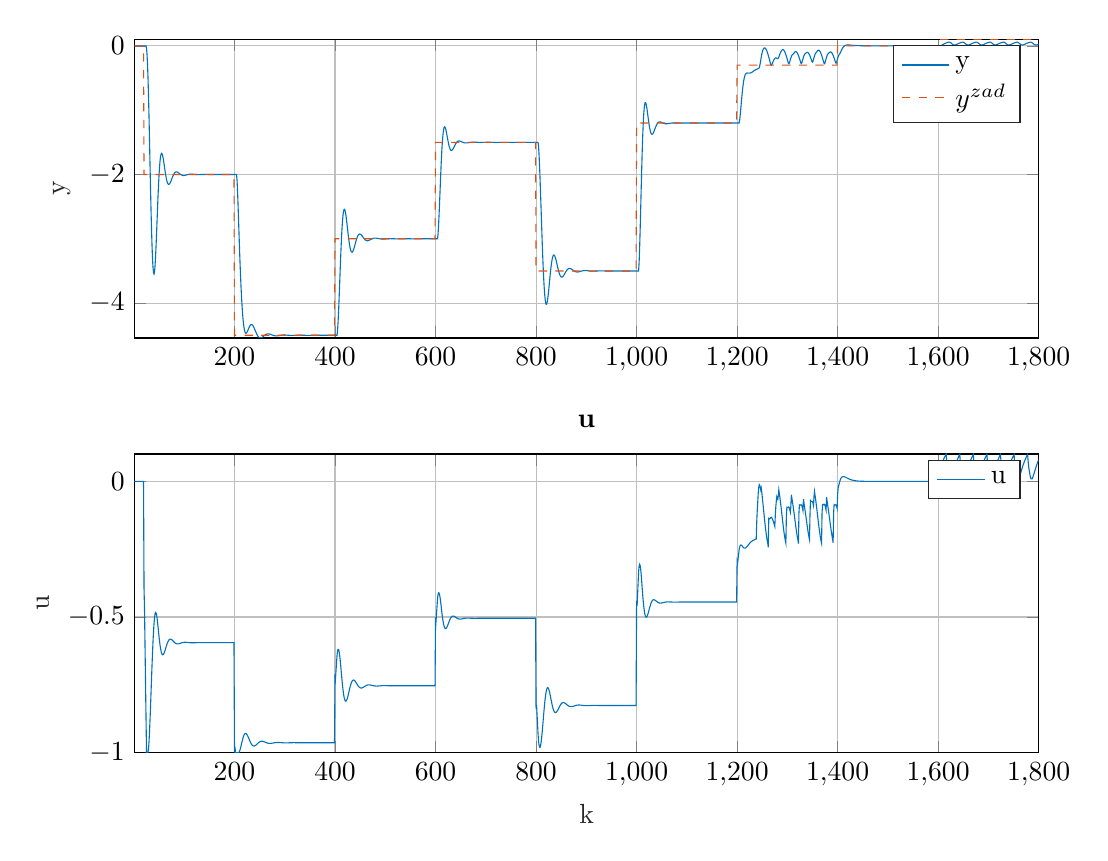
\begin{tikzpicture}

\begin{axis}[%
width=4.521in,
height=1.493in,
at={(0.758in,2.554in)},
scale only axis,
xmin=1,
xmax=1800,
ymin=-4.5419,
ymax=0.1,
ylabel style={font=\color{white!15!black}},
ylabel={y},
axis background/.style={fill=white},
xmajorgrids,
ymajorgrids,
legend style={legend cell align=left, align=left, draw=white!15!black}
]
\addplot [color=mycolor1]
  table[row sep=crcr]{%
1	0\\
2	0\\
3	0\\
4	0\\
5	0\\
6	0\\
7	0\\
8	0\\
9	0\\
10	0\\
11	0\\
12	0\\
13	0\\
14	0\\
15	0\\
16	0\\
17	0\\
18	0\\
19	0\\
20	0\\
21	0\\
22	0\\
23	0\\
24	0\\
25	-0.037705\\
26	-0.13822\\
27	-0.29676\\
28	-0.51497\\
29	-0.79316\\
30	-1.1289\\
31	-1.4987\\
32	-1.8745\\
33	-2.2376\\
34	-2.5744\\
35	-2.8732\\
36	-3.1242\\
37	-3.3203\\
38	-3.457\\
39	-3.5323\\
40	-3.547\\
41	-3.5044\\
42	-3.4103\\
43	-3.2728\\
44	-3.1018\\
45	-2.9088\\
46	-2.7054\\
47	-2.5029\\
48	-2.3114\\
49	-2.1387\\
50	-1.9907\\
51	-1.8706\\
52	-1.7797\\
53	-1.7176\\
54	-1.6824\\
55	-1.6711\\
56	-1.6804\\
57	-1.7064\\
58	-1.7452\\
59	-1.7927\\
60	-1.8454\\
61	-1.8999\\
62	-1.9534\\
63	-2.0033\\
64	-2.0477\\
65	-2.0852\\
66	-2.1148\\
67	-2.1362\\
68	-2.1493\\
69	-2.1546\\
70	-2.1527\\
71	-2.1447\\
72	-2.1316\\
73	-2.1147\\
74	-2.0953\\
75	-2.0746\\
76	-2.0538\\
77	-2.0337\\
78	-2.0152\\
79	-1.999\\
80	-1.9854\\
81	-1.9747\\
82	-1.967\\
83	-1.9621\\
84	-1.96\\
85	-1.9602\\
86	-1.9624\\
87	-1.9663\\
88	-1.9713\\
89	-1.9771\\
90	-1.9833\\
91	-1.9895\\
92	-1.9954\\
93	-2.0008\\
94	-2.0055\\
95	-2.0093\\
96	-2.0122\\
97	-2.0142\\
98	-2.0153\\
99	-2.0155\\
100	-2.0151\\
101	-2.014\\
102	-2.0124\\
103	-2.0105\\
104	-2.0084\\
105	-2.0062\\
106	-2.0041\\
107	-2.0021\\
108	-2.0003\\
109	-1.9987\\
110	-1.9974\\
111	-1.9965\\
112	-1.9959\\
113	-1.9955\\
114	-1.9954\\
115	-1.9956\\
116	-1.996\\
117	-1.9965\\
118	-1.9971\\
119	-1.9977\\
120	-1.9984\\
121	-1.9991\\
122	-1.9997\\
123	-2.0003\\
124	-2.0007\\
125	-2.0011\\
126	-2.0014\\
127	-2.0015\\
128	-2.0016\\
129	-2.0016\\
130	-2.0015\\
131	-2.0014\\
132	-2.0012\\
133	-2.001\\
134	-2.0008\\
135	-2.0005\\
136	-2.0003\\
137	-2.0001\\
138	-1.9999\\
139	-1.9998\\
140	-1.9997\\
141	-1.9996\\
142	-1.9995\\
143	-1.9995\\
144	-1.9995\\
145	-1.9995\\
146	-1.9996\\
147	-1.9996\\
148	-1.9997\\
149	-1.9998\\
150	-1.9999\\
151	-1.9999\\
152	-2\\
153	-2\\
154	-2.0001\\
155	-2.0001\\
156	-2.0002\\
157	-2.0002\\
158	-2.0002\\
159	-2.0002\\
160	-2.0002\\
161	-2.0001\\
162	-2.0001\\
163	-2.0001\\
164	-2.0001\\
165	-2\\
166	-2\\
167	-2\\
168	-2\\
169	-2\\
170	-2\\
171	-1.9999\\
172	-1.9999\\
173	-1.9999\\
174	-1.9999\\
175	-2\\
176	-2\\
177	-2\\
178	-2\\
179	-2\\
180	-2\\
181	-2\\
182	-2\\
183	-2\\
184	-2\\
185	-2\\
186	-2\\
187	-2\\
188	-2\\
189	-2\\
190	-2\\
191	-2\\
192	-2\\
193	-2\\
194	-2\\
195	-2\\
196	-2\\
197	-2\\
198	-2\\
199	-2\\
200	-2\\
201	-2\\
202	-2\\
203	-2\\
204	-2\\
205	-2.0801\\
206	-2.2427\\
207	-2.4526\\
208	-2.6856\\
209	-2.9234\\
210	-3.1541\\
211	-3.3704\\
212	-3.5682\\
213	-3.7459\\
214	-3.903\\
215	-4.0393\\
216	-4.155\\
217	-4.2505\\
218	-4.3267\\
219	-4.3847\\
220	-4.426\\
221	-4.4525\\
222	-4.4661\\
223	-4.4689\\
224	-4.4632\\
225	-4.451\\
226	-4.4346\\
227	-4.4158\\
228	-4.3963\\
229	-4.3778\\
230	-4.3614\\
231	-4.3482\\
232	-4.3387\\
233	-4.3334\\
234	-4.3325\\
235	-4.3358\\
236	-4.3431\\
237	-4.354\\
238	-4.3678\\
239	-4.3839\\
240	-4.4017\\
241	-4.4205\\
242	-4.4394\\
243	-4.458\\
244	-4.4756\\
245	-4.4917\\
246	-4.5059\\
247	-4.5179\\
248	-4.5275\\
249	-4.5347\\
250	-4.5394\\
251	-4.5418\\
252	-4.5419\\
253	-4.5402\\
254	-4.5368\\
255	-4.532\\
256	-4.5263\\
257	-4.52\\
258	-4.5133\\
259	-4.5066\\
260	-4.5002\\
261	-4.4944\\
262	-4.4892\\
263	-4.4849\\
264	-4.4816\\
265	-4.4792\\
266	-4.4779\\
267	-4.4775\\
268	-4.478\\
269	-4.4793\\
270	-4.4812\\
271	-4.4836\\
272	-4.4865\\
273	-4.4895\\
274	-4.4927\\
275	-4.4958\\
276	-4.4988\\
277	-4.5015\\
278	-4.5038\\
279	-4.5058\\
280	-4.5073\\
281	-4.5084\\
282	-4.5091\\
283	-4.5093\\
284	-4.5091\\
285	-4.5086\\
286	-4.5078\\
287	-4.5067\\
288	-4.5055\\
289	-4.5042\\
290	-4.5028\\
291	-4.5015\\
292	-4.5002\\
293	-4.4991\\
294	-4.4981\\
295	-4.4973\\
296	-4.4966\\
297	-4.4962\\
298	-4.4959\\
299	-4.4958\\
300	-4.496\\
301	-4.4962\\
302	-4.4966\\
303	-4.4971\\
304	-4.4976\\
305	-4.4982\\
306	-4.4988\\
307	-4.4994\\
308	-4.4999\\
309	-4.5004\\
310	-4.5009\\
311	-4.5012\\
312	-4.5015\\
313	-4.5017\\
314	-4.5018\\
315	-4.5018\\
316	-4.5018\\
317	-4.5016\\
318	-4.5015\\
319	-4.5013\\
320	-4.501\\
321	-4.5008\\
322	-4.5005\\
323	-4.5003\\
324	-4.5\\
325	-4.4998\\
326	-4.4996\\
327	-4.4995\\
328	-4.4993\\
329	-4.4993\\
330	-4.4992\\
331	-4.4992\\
332	-4.4992\\
333	-4.4993\\
334	-4.4994\\
335	-4.4995\\
336	-4.4996\\
337	-4.4997\\
338	-4.4998\\
339	-4.4999\\
340	-4.5\\
341	-4.5001\\
342	-4.5002\\
343	-4.5002\\
344	-4.5003\\
345	-4.5003\\
346	-4.5003\\
347	-4.5003\\
348	-4.5003\\
349	-4.5003\\
350	-4.5003\\
351	-4.5002\\
352	-4.5002\\
353	-4.5001\\
354	-4.5001\\
355	-4.5\\
356	-4.5\\
357	-4.5\\
358	-4.4999\\
359	-4.4999\\
360	-4.4999\\
361	-4.4999\\
362	-4.4998\\
363	-4.4998\\
364	-4.4999\\
365	-4.4999\\
366	-4.4999\\
367	-4.4999\\
368	-4.4999\\
369	-4.4999\\
370	-4.5\\
371	-4.5\\
372	-4.5\\
373	-4.5\\
374	-4.5\\
375	-4.5\\
376	-4.5001\\
377	-4.5001\\
378	-4.5001\\
379	-4.5001\\
380	-4.5001\\
381	-4.5001\\
382	-4.5001\\
383	-4.5\\
384	-4.5\\
385	-4.5\\
386	-4.5\\
387	-4.5\\
388	-4.5\\
389	-4.5\\
390	-4.5\\
391	-4.5\\
392	-4.5\\
393	-4.5\\
394	-4.5\\
395	-4.5\\
396	-4.5\\
397	-4.5\\
398	-4.5\\
399	-4.5\\
400	-4.5\\
401	-4.5\\
402	-4.5\\
403	-4.5\\
404	-4.5\\
405	-4.4319\\
406	-4.3057\\
407	-4.143\\
408	-3.9553\\
409	-3.7516\\
410	-3.5418\\
411	-3.3365\\
412	-3.1448\\
413	-2.9739\\
414	-2.8288\\
415	-2.7127\\
416	-2.6269\\
417	-2.5708\\
418	-2.5429\\
419	-2.5405\\
420	-2.5601\\
421	-2.598\\
422	-2.65\\
423	-2.7121\\
424	-2.7804\\
425	-2.851\\
426	-2.9208\\
427	-2.9868\\
428	-3.0467\\
429	-3.0985\\
430	-3.1409\\
431	-3.1731\\
432	-3.1949\\
433	-3.2063\\
434	-3.2081\\
435	-3.2012\\
436	-3.1867\\
437	-3.1662\\
438	-3.1412\\
439	-3.1133\\
440	-3.0839\\
441	-3.0545\\
442	-3.0265\\
443	-3.0007\\
444	-2.9781\\
445	-2.9593\\
446	-2.9446\\
447	-2.9341\\
448	-2.9279\\
449	-2.9256\\
450	-2.9268\\
451	-2.9311\\
452	-2.938\\
453	-2.9468\\
454	-2.9569\\
455	-2.9677\\
456	-2.9786\\
457	-2.9893\\
458	-2.9992\\
459	-3.008\\
460	-3.0155\\
461	-3.0215\\
462	-3.0258\\
463	-3.0286\\
464	-3.0298\\
465	-3.0297\\
466	-3.0282\\
467	-3.0258\\
468	-3.0225\\
469	-3.0187\\
470	-3.0145\\
471	-3.0102\\
472	-3.0059\\
473	-3.0019\\
474	-2.9983\\
475	-2.9952\\
476	-2.9927\\
477	-2.9908\\
478	-2.9895\\
479	-2.9888\\
480	-2.9887\\
481	-2.9891\\
482	-2.9899\\
483	-2.9911\\
484	-2.9925\\
485	-2.994\\
486	-2.9957\\
487	-2.9973\\
488	-2.9989\\
489	-3.0003\\
490	-3.0016\\
491	-3.0026\\
492	-3.0034\\
493	-3.004\\
494	-3.0043\\
495	-3.0044\\
496	-3.0043\\
497	-3.004\\
498	-3.0036\\
499	-3.0031\\
500	-3.0025\\
501	-3.0019\\
502	-3.0012\\
503	-3.0006\\
504	-3.0001\\
505	-2.9996\\
506	-2.9991\\
507	-2.9988\\
508	-2.9985\\
509	-2.9984\\
510	-2.9983\\
511	-2.9983\\
512	-2.9984\\
513	-2.9986\\
514	-2.9987\\
515	-2.999\\
516	-2.9992\\
517	-2.9994\\
518	-2.9997\\
519	-2.9999\\
520	-3.0001\\
521	-3.0003\\
522	-3.0004\\
523	-3.0005\\
524	-3.0006\\
525	-3.0006\\
526	-3.0007\\
527	-3.0006\\
528	-3.0006\\
529	-3.0005\\
530	-3.0004\\
531	-3.0003\\
532	-3.0002\\
533	-3.0001\\
534	-3.0001\\
535	-3\\
536	-2.9999\\
537	-2.9998\\
538	-2.9998\\
539	-2.9998\\
540	-2.9998\\
541	-2.9997\\
542	-2.9998\\
543	-2.9998\\
544	-2.9998\\
545	-2.9998\\
546	-2.9999\\
547	-2.9999\\
548	-2.9999\\
549	-3\\
550	-3\\
551	-3\\
552	-3.0001\\
553	-3.0001\\
554	-3.0001\\
555	-3.0001\\
556	-3.0001\\
557	-3.0001\\
558	-3.0001\\
559	-3.0001\\
560	-3.0001\\
561	-3.0001\\
562	-3\\
563	-3\\
564	-3\\
565	-3\\
566	-3\\
567	-3\\
568	-3\\
569	-3\\
570	-3\\
571	-3\\
572	-3\\
573	-3\\
574	-3\\
575	-3\\
576	-3\\
577	-3\\
578	-3\\
579	-3\\
580	-3\\
581	-3\\
582	-3\\
583	-3\\
584	-3\\
585	-3\\
586	-3\\
587	-3\\
588	-3\\
589	-3\\
590	-3\\
591	-3\\
592	-3\\
593	-3\\
594	-3\\
595	-3\\
596	-3\\
597	-3\\
598	-3\\
599	-3\\
600	-3\\
601	-3\\
602	-3\\
603	-3\\
604	-3\\
605	-2.9262\\
606	-2.7955\\
607	-2.631\\
608	-2.4459\\
609	-2.2501\\
610	-2.0544\\
611	-1.8697\\
612	-1.704\\
613	-1.5627\\
614	-1.4488\\
615	-1.363\\
616	-1.3044\\
617	-1.2709\\
618	-1.2593\\
619	-1.266\\
620	-1.2872\\
621	-1.3192\\
622	-1.3582\\
623	-1.401\\
624	-1.4446\\
625	-1.4866\\
626	-1.5249\\
627	-1.558\\
628	-1.5849\\
629	-1.6051\\
630	-1.6185\\
631	-1.6252\\
632	-1.6259\\
633	-1.6214\\
634	-1.6125\\
635	-1.6003\\
636	-1.5858\\
637	-1.5701\\
638	-1.5541\\
639	-1.5386\\
640	-1.5242\\
641	-1.5115\\
642	-1.5007\\
643	-1.4921\\
644	-1.4858\\
645	-1.4815\\
646	-1.4792\\
647	-1.4787\\
648	-1.4796\\
649	-1.4816\\
650	-1.4845\\
651	-1.488\\
652	-1.4917\\
653	-1.4954\\
654	-1.4989\\
655	-1.502\\
656	-1.5047\\
657	-1.5069\\
658	-1.5084\\
659	-1.5094\\
660	-1.5099\\
661	-1.5098\\
662	-1.5094\\
663	-1.5086\\
664	-1.5076\\
665	-1.5064\\
666	-1.5051\\
667	-1.5039\\
668	-1.5026\\
669	-1.5015\\
670	-1.5005\\
671	-1.4997\\
672	-1.4991\\
673	-1.4986\\
674	-1.4983\\
675	-1.4982\\
676	-1.4982\\
677	-1.4983\\
678	-1.4985\\
679	-1.4987\\
680	-1.499\\
681	-1.4993\\
682	-1.4996\\
683	-1.4999\\
684	-1.5002\\
685	-1.5004\\
686	-1.5006\\
687	-1.5007\\
688	-1.5007\\
689	-1.5008\\
690	-1.5008\\
691	-1.5007\\
692	-1.5007\\
693	-1.5006\\
694	-1.5005\\
695	-1.5004\\
696	-1.5003\\
697	-1.5002\\
698	-1.5001\\
699	-1.5\\
700	-1.5\\
701	-1.4999\\
702	-1.4999\\
703	-1.4999\\
704	-1.4998\\
705	-1.4998\\
706	-1.4999\\
707	-1.4999\\
708	-1.4999\\
709	-1.4999\\
710	-1.4999\\
711	-1.5\\
712	-1.5\\
713	-1.5\\
714	-1.5\\
715	-1.5\\
716	-1.5001\\
717	-1.5001\\
718	-1.5001\\
719	-1.5001\\
720	-1.5001\\
721	-1.5001\\
722	-1.5\\
723	-1.5\\
724	-1.5\\
725	-1.5\\
726	-1.5\\
727	-1.5\\
728	-1.5\\
729	-1.5\\
730	-1.5\\
731	-1.5\\
732	-1.5\\
733	-1.5\\
734	-1.5\\
735	-1.5\\
736	-1.5\\
737	-1.5\\
738	-1.5\\
739	-1.5\\
740	-1.5\\
741	-1.5\\
742	-1.5\\
743	-1.5\\
744	-1.5\\
745	-1.5\\
746	-1.5\\
747	-1.5\\
748	-1.5\\
749	-1.5\\
750	-1.5\\
751	-1.5\\
752	-1.5\\
753	-1.5\\
754	-1.5\\
755	-1.5\\
756	-1.5\\
757	-1.5\\
758	-1.5\\
759	-1.5\\
760	-1.5\\
761	-1.5\\
762	-1.5\\
763	-1.5\\
764	-1.5\\
765	-1.5\\
766	-1.5\\
767	-1.5\\
768	-1.5\\
769	-1.5\\
770	-1.5\\
771	-1.5\\
772	-1.5\\
773	-1.5\\
774	-1.5\\
775	-1.5\\
776	-1.5\\
777	-1.5\\
778	-1.5\\
779	-1.5\\
780	-1.5\\
781	-1.5\\
782	-1.5\\
783	-1.5\\
784	-1.5\\
785	-1.5\\
786	-1.5\\
787	-1.5\\
788	-1.5\\
789	-1.5\\
790	-1.5\\
791	-1.5\\
792	-1.5\\
793	-1.5\\
794	-1.5\\
795	-1.5\\
796	-1.5\\
797	-1.5\\
798	-1.5\\
799	-1.5\\
800	-1.5\\
801	-1.5\\
802	-1.5\\
803	-1.5\\
804	-1.5\\
805	-1.567\\
806	-1.7013\\
807	-1.877\\
808	-2.0809\\
809	-2.3039\\
810	-2.5375\\
811	-2.7728\\
812	-3.0019\\
813	-3.2178\\
814	-3.4145\\
815	-3.5876\\
816	-3.7335\\
817	-3.8499\\
818	-3.9358\\
819	-3.9911\\
820	-4.0172\\
821	-4.0161\\
822	-3.9909\\
823	-3.9454\\
824	-3.8839\\
825	-3.8108\\
826	-3.7307\\
827	-3.6481\\
828	-3.5669\\
829	-3.4908\\
830	-3.4227\\
831	-3.3645\\
832	-3.3179\\
833	-3.2836\\
834	-3.2617\\
835	-3.2518\\
836	-3.2529\\
837	-3.2638\\
838	-3.283\\
839	-3.3087\\
840	-3.3393\\
841	-3.3729\\
842	-3.4078\\
843	-3.4426\\
844	-3.4758\\
845	-3.5062\\
846	-3.533\\
847	-3.5554\\
848	-3.573\\
849	-3.5856\\
850	-3.5932\\
851	-3.596\\
852	-3.5945\\
853	-3.5892\\
854	-3.5807\\
855	-3.5697\\
856	-3.5569\\
857	-3.5432\\
858	-3.5291\\
859	-3.5153\\
860	-3.5024\\
861	-3.4908\\
862	-3.4808\\
863	-3.4727\\
864	-3.4666\\
865	-3.4626\\
866	-3.4605\\
867	-3.4604\\
868	-3.4619\\
869	-3.4648\\
870	-3.4688\\
871	-3.4737\\
872	-3.4792\\
873	-3.4849\\
874	-3.4906\\
875	-3.4961\\
876	-3.5011\\
877	-3.5056\\
878	-3.5093\\
879	-3.5122\\
880	-3.5143\\
881	-3.5156\\
882	-3.5161\\
883	-3.5159\\
884	-3.515\\
885	-3.5136\\
886	-3.5118\\
887	-3.5096\\
888	-3.5074\\
889	-3.505\\
890	-3.5027\\
891	-3.5006\\
892	-3.4986\\
893	-3.497\\
894	-3.4956\\
895	-3.4946\\
896	-3.4939\\
897	-3.4935\\
898	-3.4935\\
899	-3.4937\\
900	-3.4941\\
901	-3.4948\\
902	-3.4956\\
903	-3.4965\\
904	-3.4974\\
905	-3.4984\\
906	-3.4993\\
907	-3.5001\\
908	-3.5009\\
909	-3.5015\\
910	-3.502\\
911	-3.5024\\
912	-3.5026\\
913	-3.5027\\
914	-3.5026\\
915	-3.5025\\
916	-3.5023\\
917	-3.502\\
918	-3.5016\\
919	-3.5012\\
920	-3.5009\\
921	-3.5005\\
922	-3.5001\\
923	-3.4998\\
924	-3.4995\\
925	-3.4993\\
926	-3.4991\\
927	-3.499\\
928	-3.4989\\
929	-3.4989\\
930	-3.4989\\
931	-3.499\\
932	-3.4991\\
933	-3.4993\\
934	-3.4994\\
935	-3.4996\\
936	-3.4997\\
937	-3.4999\\
938	-3.5\\
939	-3.5001\\
940	-3.5002\\
941	-3.5003\\
942	-3.5004\\
943	-3.5004\\
944	-3.5004\\
945	-3.5004\\
946	-3.5004\\
947	-3.5004\\
948	-3.5003\\
949	-3.5003\\
950	-3.5002\\
951	-3.5001\\
952	-3.5001\\
953	-3.5\\
954	-3.5\\
955	-3.4999\\
956	-3.4999\\
957	-3.4999\\
958	-3.4998\\
959	-3.4998\\
960	-3.4998\\
961	-3.4998\\
962	-3.4998\\
963	-3.4999\\
964	-3.4999\\
965	-3.4999\\
966	-3.4999\\
967	-3.5\\
968	-3.5\\
969	-3.5\\
970	-3.5\\
971	-3.5\\
972	-3.5001\\
973	-3.5001\\
974	-3.5001\\
975	-3.5001\\
976	-3.5001\\
977	-3.5001\\
978	-3.5001\\
979	-3.5001\\
980	-3.5\\
981	-3.5\\
982	-3.5\\
983	-3.5\\
984	-3.5\\
985	-3.5\\
986	-3.5\\
987	-3.5\\
988	-3.5\\
989	-3.5\\
990	-3.5\\
991	-3.5\\
992	-3.5\\
993	-3.5\\
994	-3.5\\
995	-3.5\\
996	-3.5\\
997	-3.5\\
998	-3.5\\
999	-3.5\\
1000	-3.5\\
1001	-3.5\\
1002	-3.5\\
1003	-3.5\\
1004	-3.5\\
1005	-3.3746\\
1006	-3.1592\\
1007	-2.8907\\
1008	-2.5911\\
1009	-2.2772\\
1010	-1.9699\\
1011	-1.6876\\
1012	-1.4432\\
1013	-1.2434\\
1014	-1.0904\\
1015	-0.98243\\
1016	-0.91576\\
1017	-0.88498\\
1018	-0.88403\\
1019	-0.90662\\
1020	-0.94665\\
1021	-0.9984\\
1022	-1.0567\\
1023	-1.1171\\
1024	-1.1757\\
1025	-1.2296\\
1026	-1.2766\\
1027	-1.315\\
1028	-1.344\\
1029	-1.3635\\
1030	-1.3737\\
1031	-1.3755\\
1032	-1.3699\\
1033	-1.3582\\
1034	-1.3421\\
1035	-1.3229\\
1036	-1.3021\\
1037	-1.2809\\
1038	-1.2605\\
1039	-1.2416\\
1040	-1.225\\
1041	-1.211\\
1042	-1.1999\\
1043	-1.1916\\
1044	-1.1861\\
1045	-1.183\\
1046	-1.182\\
1047	-1.1828\\
1048	-1.1849\\
1049	-1.1879\\
1050	-1.1915\\
1051	-1.1954\\
1052	-1.1992\\
1053	-1.2028\\
1054	-1.2059\\
1055	-1.2084\\
1056	-1.2103\\
1057	-1.2116\\
1058	-1.2123\\
1059	-1.2124\\
1060	-1.212\\
1061	-1.2112\\
1062	-1.2102\\
1063	-1.2089\\
1064	-1.2075\\
1065	-1.2061\\
1066	-1.2047\\
1067	-1.2035\\
1068	-1.2023\\
1069	-1.2014\\
1070	-1.2006\\
1071	-1.2\\
1072	-1.1996\\
1073	-1.1993\\
1074	-1.1992\\
1075	-1.1992\\
1076	-1.1993\\
1077	-1.1994\\
1078	-1.1996\\
1079	-1.1999\\
1080	-1.2001\\
1081	-1.2003\\
1082	-1.2005\\
1083	-1.2006\\
1084	-1.2008\\
1085	-1.2008\\
1086	-1.2009\\
1087	-1.2009\\
1088	-1.2009\\
1089	-1.2008\\
1090	-1.2007\\
1091	-1.2007\\
1092	-1.2006\\
1093	-1.2005\\
1094	-1.2004\\
1095	-1.2003\\
1096	-1.2002\\
1097	-1.2001\\
1098	-1.2001\\
1099	-1.2\\
1100	-1.2\\
1101	-1.2\\
1102	-1.2\\
1103	-1.2\\
1104	-1.2\\
1105	-1.2\\
1106	-1.2\\
1107	-1.2\\
1108	-1.2\\
1109	-1.2\\
1110	-1.2\\
1111	-1.2001\\
1112	-1.2001\\
1113	-1.2001\\
1114	-1.2001\\
1115	-1.2001\\
1116	-1.2001\\
1117	-1.2001\\
1118	-1.2001\\
1119	-1.2\\
1120	-1.2\\
1121	-1.2\\
1122	-1.2\\
1123	-1.2\\
1124	-1.2\\
1125	-1.2\\
1126	-1.2\\
1127	-1.2\\
1128	-1.2\\
1129	-1.2\\
1130	-1.2\\
1131	-1.2\\
1132	-1.2\\
1133	-1.2\\
1134	-1.2\\
1135	-1.2\\
1136	-1.2\\
1137	-1.2\\
1138	-1.2\\
1139	-1.2\\
1140	-1.2\\
1141	-1.2\\
1142	-1.2\\
1143	-1.2\\
1144	-1.2\\
1145	-1.2\\
1146	-1.2\\
1147	-1.2\\
1148	-1.2\\
1149	-1.2\\
1150	-1.2\\
1151	-1.2\\
1152	-1.2\\
1153	-1.2\\
1154	-1.2\\
1155	-1.2\\
1156	-1.2\\
1157	-1.2\\
1158	-1.2\\
1159	-1.2\\
1160	-1.2\\
1161	-1.2\\
1162	-1.2\\
1163	-1.2\\
1164	-1.2\\
1165	-1.2\\
1166	-1.2\\
1167	-1.2\\
1168	-1.2\\
1169	-1.2\\
1170	-1.2\\
1171	-1.2\\
1172	-1.2\\
1173	-1.2\\
1174	-1.2\\
1175	-1.2\\
1176	-1.2\\
1177	-1.2\\
1178	-1.2\\
1179	-1.2\\
1180	-1.2\\
1181	-1.2\\
1182	-1.2\\
1183	-1.2\\
1184	-1.2\\
1185	-1.2\\
1186	-1.2\\
1187	-1.2\\
1188	-1.2\\
1189	-1.2\\
1190	-1.2\\
1191	-1.2\\
1192	-1.2\\
1193	-1.2\\
1194	-1.2\\
1195	-1.2\\
1196	-1.2\\
1197	-1.2\\
1198	-1.2\\
1199	-1.2\\
1200	-1.2\\
1201	-1.2\\
1202	-1.2\\
1203	-1.2\\
1204	-1.2\\
1205	-1.1595\\
1206	-1.0904\\
1207	-1.0075\\
1208	-0.91874\\
1209	-0.82958\\
1210	-0.7449\\
1211	-0.66863\\
1212	-0.60311\\
1213	-0.54926\\
1214	-0.50692\\
1215	-0.4752\\
1216	-0.45274\\
1217	-0.43794\\
1218	-0.42911\\
1219	-0.42465\\
1220	-0.42312\\
1221	-0.42329\\
1222	-0.42418\\
1223	-0.42504\\
1224	-0.42536\\
1225	-0.42481\\
1226	-0.42326\\
1227	-0.4207\\
1228	-0.41721\\
1229	-0.41295\\
1230	-0.40811\\
1231	-0.40289\\
1232	-0.39746\\
1233	-0.392\\
1234	-0.38665\\
1235	-0.38152\\
1236	-0.37667\\
1237	-0.37216\\
1238	-0.36799\\
1239	-0.36418\\
1240	-0.3607\\
1241	-0.35754\\
1242	-0.35465\\
1243	-0.352\\
1244	-0.33925\\
1245	-0.31168\\
1246	-0.27279\\
1247	-0.22691\\
1248	-0.17963\\
1249	-0.13595\\
1250	-0.099474\\
1251	-0.071889\\
1252	-0.053136\\
1253	-0.040906\\
1254	-0.034055\\
1255	-0.032874\\
1256	-0.037108\\
1257	-0.04626\\
1258	-0.05979\\
1259	-0.07719\\
1260	-0.097977\\
1261	-0.12166\\
1262	-0.14772\\
1263	-0.17559\\
1264	-0.20468\\
1265	-0.23431\\
1266	-0.26378\\
1267	-0.29346\\
1268	-0.30264\\
1269	-0.29368\\
1270	-0.27665\\
1271	-0.25719\\
1272	-0.23808\\
1273	-0.22095\\
1274	-0.20697\\
1275	-0.19672\\
1276	-0.19034\\
1277	-0.18767\\
1278	-0.18837\\
1279	-0.19202\\
1280	-0.19814\\
1281	-0.19925\\
1282	-0.19086\\
1283	-0.17418\\
1284	-0.15242\\
1285	-0.13053\\
1286	-0.11213\\
1287	-0.096708\\
1288	-0.081911\\
1289	-0.069305\\
1290	-0.061343\\
1291	-0.058714\\
1292	-0.061303\\
1293	-0.06872\\
1294	-0.080516\\
1295	-0.096216\\
1296	-0.11532\\
1297	-0.1373\\
1298	-0.16162\\
1299	-0.18769\\
1300	-0.21488\\
1301	-0.24254\\
1302	-0.26998\\
1303	-0.27847\\
1304	-0.26473\\
1305	-0.23984\\
1306	-0.21251\\
1307	-0.18699\\
1308	-0.16536\\
1309	-0.1487\\
1310	-0.13745\\
1311	-0.13149\\
1312	-0.12636\\
1313	-0.11635\\
1314	-0.10441\\
1315	-0.095081\\
1316	-0.09009\\
1317	-0.089818\\
1318	-0.094143\\
1319	-0.10278\\
1320	-0.11535\\
1321	-0.13137\\
1322	-0.15033\\
1323	-0.17169\\
1324	-0.19486\\
1325	-0.21923\\
1326	-0.24419\\
1327	-0.27007\\
1328	-0.27573\\
1329	-0.25877\\
1330	-0.23122\\
1331	-0.20195\\
1332	-0.17518\\
1333	-0.15287\\
1334	-0.13602\\
1335	-0.12494\\
1336	-0.11941\\
1337	-0.11298\\
1338	-0.10588\\
1339	-0.10155\\
1340	-0.10128\\
1341	-0.10528\\
1342	-0.11334\\
1343	-0.12512\\
1344	-0.14023\\
1345	-0.15819\\
1346	-0.17847\\
1347	-0.20051\\
1348	-0.22371\\
1349	-0.24747\\
1350	-0.25467\\
1351	-0.23902\\
1352	-0.21159\\
1353	-0.18223\\
1354	-0.15562\\
1355	-0.1338\\
1356	-0.11766\\
1357	-0.10743\\
1358	-0.098182\\
1359	-0.086802\\
1360	-0.076108\\
1361	-0.069165\\
1362	-0.067021\\
1363	-0.069745\\
1364	-0.077073\\
1365	-0.088639\\
1366	-0.10401\\
1367	-0.12271\\
1368	-0.14422\\
1369	-0.16799\\
1370	-0.19343\\
1371	-0.21994\\
1372	-0.24684\\
1373	-0.27346\\
1374	-0.27879\\
1375	-0.26109\\
1376	-0.23268\\
1377	-0.20256\\
1378	-0.17499\\
1379	-0.15199\\
1380	-0.13459\\
1381	-0.12308\\
1382	-0.11724\\
1383	-0.11005\\
1384	-0.10175\\
1385	-0.096136\\
1386	-0.094675\\
1387	-0.097638\\
1388	-0.10483\\
1389	-0.11593\\
1390	-0.13054\\
1391	-0.1482\\
1392	-0.16838\\
1393	-0.19052\\
1394	-0.21403\\
1395	-0.2383\\
1396	-0.26367\\
1397	-0.26941\\
1398	-0.25306\\
1399	-0.22642\\
1400	-0.19815\\
1401	-0.17238\\
1402	-0.151\\
1403	-0.13498\\
1404	-0.1246\\
1405	-0.11289\\
1406	-0.096778\\
1407	-0.078866\\
1408	-0.061567\\
1409	-0.045959\\
1410	-0.032434\\
1411	-0.02108\\
1412	-0.011822\\
1413	-0.0044753\\
1414	0.0012044\\
1415	0.0054747\\
1416	0.0085819\\
1417	0.010748\\
1418	0.012166\\
1419	0.012999\\
1420	0.013381\\
1421	0.013422\\
1422	0.013208\\
1423	0.01281\\
1424	0.012283\\
1425	0.011669\\
1426	0.011001\\
1427	0.010304\\
1428	0.0095987\\
1429	0.0088984\\
1430	0.0082141\\
1431	0.0075536\\
1432	0.0069221\\
1433	0.0063234\\
1434	0.0057596\\
1435	0.0052318\\
1436	0.0047402\\
1437	0.0042844\\
1438	0.0038636\\
1439	0.0034765\\
1440	0.0031217\\
1441	0.0027975\\
1442	0.0025021\\
1443	0.0022337\\
1444	0.0019905\\
1445	0.0017707\\
1446	0.0015725\\
1447	0.0013942\\
1448	0.0012341\\
1449	0.0010907\\
1450	0.00096245\\
1451	0.00084802\\
1452	0.00074609\\
1453	0.00065547\\
1454	0.00057504\\
1455	0.00050377\\
1456	0.00044073\\
1457	0.00038505\\
1458	0.00033596\\
1459	0.00029273\\
1460	0.00025474\\
1461	0.00022138\\
1462	0.00019214\\
1463	0.00016655\\
1464	0.00014418\\
1465	0.00012465\\
1466	0.00010763\\
1467	9.2807e-05\\
1468	7.9923e-05\\
1469	6.8736e-05\\
1470	5.9037e-05\\
1471	5.0637e-05\\
1472	4.3372e-05\\
1473	3.7097e-05\\
1474	3.1685e-05\\
1475	2.7023e-05\\
1476	2.3012e-05\\
1477	1.9565e-05\\
1478	1.6609e-05\\
1479	1.4076e-05\\
1480	1.1908e-05\\
1481	1.0056e-05\\
1482	8.4765e-06\\
1483	7.1308e-06\\
1484	5.9863e-06\\
1485	5.0144e-06\\
1486	4.1904e-06\\
1487	3.4931e-06\\
1488	2.904e-06\\
1489	2.4072e-06\\
1490	1.9891e-06\\
1491	1.638e-06\\
1492	1.3438e-06\\
1493	1.0978e-06\\
1494	8.9264e-07\\
1495	7.2198e-07\\
1496	5.8043e-07\\
1497	4.6339e-07\\
1498	3.6694e-07\\
1499	2.8775e-07\\
1500	2.23e-07\\
1501	1.703e-07\\
1502	1.2763e-07\\
1503	9.3286e-08\\
1504	6.5825e-08\\
1505	4.4042e-08\\
1506	2.6925e-08\\
1507	1.3626e-08\\
1508	3.4374e-09\\
1509	-4.2299e-09\\
1510	-9.8651e-09\\
1511	-1.3873e-08\\
1512	-1.6589e-08\\
1513	-1.8287e-08\\
1514	-1.9192e-08\\
1515	-1.9488e-08\\
1516	-1.9324e-08\\
1517	-1.882e-08\\
1518	-1.8073e-08\\
1519	-1.7158e-08\\
1520	-1.6137e-08\\
1521	-1.5057e-08\\
1522	-1.3953e-08\\
1523	-1.2855e-08\\
1524	-1.1782e-08\\
1525	-1.0749e-08\\
1526	-9.7657e-09\\
1527	-8.8397e-09\\
1528	-7.9744e-09\\
1529	-7.1715e-09\\
1530	-6.431e-09\\
1531	-5.7517e-09\\
1532	-5.1314e-09\\
1533	-4.5674e-09\\
1534	-4.0565e-09\\
1535	-3.5953e-09\\
1536	-3.1803e-09\\
1537	-2.8079e-09\\
1538	-2.4747e-09\\
1539	-2.1773e-09\\
1540	-1.9125e-09\\
1541	-1.6772e-09\\
1542	-1.4686e-09\\
1543	-1.284e-09\\
1544	-1.1209e-09\\
1545	-9.7715e-10\\
1546	-8.5062e-10\\
1547	-7.3944e-10\\
1548	-6.4191e-10\\
1549	-5.5649e-10\\
1550	-4.8179e-10\\
1551	-4.1655e-10\\
1552	-3.5966e-10\\
1553	-3.1013e-10\\
1554	-2.6706e-10\\
1555	-2.2966e-10\\
1556	-1.9723e-10\\
1557	-1.6914e-10\\
1558	-1.4485e-10\\
1559	-1.2387e-10\\
1560	-1.0578e-10\\
1561	-9.0197e-11\\
1562	-7.6791e-11\\
1563	-6.5275e-11\\
1564	-5.5397e-11\\
1565	-4.6935e-11\\
1566	-3.9696e-11\\
1567	-3.3513e-11\\
1568	-2.8239e-11\\
1569	-2.3747e-11\\
1570	-1.9928e-11\\
1571	-1.6686e-11\\
1572	-1.3938e-11\\
1573	-1.1614e-11\\
1574	-9.6502e-12\\
1575	-7.9951e-12\\
1576	-6.6027e-12\\
1577	-5.4338e-12\\
1578	-4.4546e-12\\
1579	-3.6362e-12\\
1580	-2.954e-12\\
1581	-2.3868e-12\\
1582	-1.9167e-12\\
1583	-1.5281e-12\\
1584	-1.2081e-12\\
1585	-9.4556e-13\\
1586	-7.3106e-13\\
1587	-5.5663e-13\\
1588	-4.1554e-13\\
1589	-3.0209e-13\\
1590	-2.1151e-13\\
1591	-1.3976e-13\\
1592	-8.3494e-14\\
1593	-3.9874e-14\\
1594	-6.5513e-15\\
1595	1.8433e-14\\
1596	3.6703e-14\\
1597	4.9606e-14\\
1598	5.825e-14\\
1599	6.3547e-14\\
1600	6.6242e-14\\
1601	6.6945e-14\\
1602	6.6146e-14\\
1603	6.4244e-14\\
1604	6.1557e-14\\
1605	0.0012443\\
1606	0.0041234\\
1607	0.0078733\\
1608	0.012148\\
1609	0.01669\\
1610	0.021308\\
1611	0.025852\\
1612	0.030213\\
1613	0.034325\\
1614	0.038151\\
1615	0.041676\\
1616	0.044905\\
1617	0.047849\\
1618	0.050529\\
1619	0.052967\\
1620	0.055189\\
1621	0.057217\\
1622	0.05831\\
1623	0.057008\\
1624	0.053454\\
1625	0.048012\\
1626	0.041143\\
1627	0.033819\\
1628	0.026886\\
1629	0.020983\\
1630	0.016438\\
1631	0.013456\\
1632	0.01214\\
1633	0.012331\\
1634	0.013762\\
1635	0.016136\\
1636	0.019172\\
1637	0.022627\\
1638	0.026298\\
1639	0.030029\\
1640	0.033704\\
1641	0.037243\\
1642	0.040594\\
1643	0.043731\\
1644	0.046643\\
1645	0.049331\\
1646	0.051803\\
1647	0.054074\\
1648	0.056159\\
1649	0.057309\\
1650	0.056086\\
1651	0.052632\\
1652	0.047647\\
1653	0.04161\\
1654	0.034922\\
1655	0.028308\\
1656	0.022471\\
1657	0.017836\\
1658	0.014684\\
1659	0.01317\\
1660	0.013165\\
1661	0.014415\\
1662	0.01663\\
1663	0.019534\\
1664	0.022881\\
1665	0.026468\\
1666	0.030133\\
1667	0.033758\\
1668	0.037261\\
1669	0.040587\\
1670	0.043707\\
1671	0.046608\\
1672	0.049289\\
1673	0.051758\\
1674	0.054028\\
1675	0.056113\\
1676	0.057264\\
1677	0.056043\\
1678	0.052594\\
1679	0.047614\\
1680	0.041582\\
1681	0.0349\\
1682	0.028292\\
1683	0.022459\\
1684	0.017829\\
1685	0.01468\\
1686	0.013168\\
1687	0.013165\\
1688	0.014416\\
1689	0.016633\\
1690	0.019537\\
1691	0.022884\\
1692	0.026471\\
1693	0.030136\\
1694	0.033762\\
1695	0.037264\\
1696	0.04059\\
1697	0.04371\\
1698	0.046611\\
1699	0.049292\\
1700	0.05176\\
1701	0.05403\\
1702	0.056115\\
1703	0.057266\\
1704	0.056045\\
1705	0.052595\\
1706	0.047615\\
1707	0.041583\\
1708	0.034901\\
1709	0.028292\\
1710	0.02246\\
1711	0.017829\\
1712	0.01468\\
1713	0.013168\\
1714	0.013165\\
1715	0.014416\\
1716	0.016633\\
1717	0.019537\\
1718	0.022884\\
1719	0.026471\\
1720	0.030136\\
1721	0.033762\\
1722	0.037264\\
1723	0.04059\\
1724	0.04371\\
1725	0.046611\\
1726	0.049291\\
1727	0.05176\\
1728	0.054029\\
1729	0.056115\\
1730	0.057266\\
1731	0.056044\\
1732	0.052595\\
1733	0.047615\\
1734	0.041583\\
1735	0.034901\\
1736	0.028292\\
1737	0.02246\\
1738	0.017829\\
1739	0.01468\\
1740	0.013168\\
1741	0.013165\\
1742	0.014416\\
1743	0.016633\\
1744	0.019537\\
1745	0.022884\\
1746	0.026471\\
1747	0.030136\\
1748	0.033762\\
1749	0.037264\\
1750	0.04059\\
1751	0.04371\\
1752	0.046611\\
1753	0.049291\\
1754	0.05176\\
1755	0.054029\\
1756	0.056115\\
1757	0.057266\\
1758	0.056044\\
1759	0.052595\\
1760	0.047615\\
1761	0.041583\\
1762	0.034901\\
1763	0.028292\\
1764	0.02246\\
1765	0.017829\\
1766	0.01468\\
1767	0.013168\\
1768	0.013165\\
1769	0.014416\\
1770	0.016633\\
1771	0.019537\\
1772	0.022884\\
1773	0.026471\\
1774	0.030136\\
1775	0.033762\\
1776	0.037264\\
1777	0.04059\\
1778	0.04371\\
1779	0.046611\\
1780	0.049291\\
1781	0.05176\\
1782	0.054029\\
1783	0.056115\\
1784	0.057266\\
1785	0.056044\\
1786	0.052595\\
1787	0.047615\\
1788	0.041583\\
1789	0.034901\\
1790	0.028292\\
1791	0.02246\\
1792	0.017829\\
1793	0.01468\\
1794	0.013168\\
1795	0.013165\\
1796	0.014416\\
1797	0.016633\\
1798	0.019537\\
1799	0.022884\\
1800	0.026471\\
};
\addlegendentry{y}

\addplot [color=mycolor2, dashed]
  table[row sep=crcr]{%
1	0\\
2	0\\
3	0\\
4	0\\
5	0\\
6	0\\
7	0\\
8	0\\
9	0\\
10	0\\
11	0\\
12	0\\
13	0\\
14	0\\
15	0\\
16	0\\
17	0\\
18	0\\
19	0\\
20	-2\\
21	-2\\
22	-2\\
23	-2\\
24	-2\\
25	-2\\
26	-2\\
27	-2\\
28	-2\\
29	-2\\
30	-2\\
31	-2\\
32	-2\\
33	-2\\
34	-2\\
35	-2\\
36	-2\\
37	-2\\
38	-2\\
39	-2\\
40	-2\\
41	-2\\
42	-2\\
43	-2\\
44	-2\\
45	-2\\
46	-2\\
47	-2\\
48	-2\\
49	-2\\
50	-2\\
51	-2\\
52	-2\\
53	-2\\
54	-2\\
55	-2\\
56	-2\\
57	-2\\
58	-2\\
59	-2\\
60	-2\\
61	-2\\
62	-2\\
63	-2\\
64	-2\\
65	-2\\
66	-2\\
67	-2\\
68	-2\\
69	-2\\
70	-2\\
71	-2\\
72	-2\\
73	-2\\
74	-2\\
75	-2\\
76	-2\\
77	-2\\
78	-2\\
79	-2\\
80	-2\\
81	-2\\
82	-2\\
83	-2\\
84	-2\\
85	-2\\
86	-2\\
87	-2\\
88	-2\\
89	-2\\
90	-2\\
91	-2\\
92	-2\\
93	-2\\
94	-2\\
95	-2\\
96	-2\\
97	-2\\
98	-2\\
99	-2\\
100	-2\\
101	-2\\
102	-2\\
103	-2\\
104	-2\\
105	-2\\
106	-2\\
107	-2\\
108	-2\\
109	-2\\
110	-2\\
111	-2\\
112	-2\\
113	-2\\
114	-2\\
115	-2\\
116	-2\\
117	-2\\
118	-2\\
119	-2\\
120	-2\\
121	-2\\
122	-2\\
123	-2\\
124	-2\\
125	-2\\
126	-2\\
127	-2\\
128	-2\\
129	-2\\
130	-2\\
131	-2\\
132	-2\\
133	-2\\
134	-2\\
135	-2\\
136	-2\\
137	-2\\
138	-2\\
139	-2\\
140	-2\\
141	-2\\
142	-2\\
143	-2\\
144	-2\\
145	-2\\
146	-2\\
147	-2\\
148	-2\\
149	-2\\
150	-2\\
151	-2\\
152	-2\\
153	-2\\
154	-2\\
155	-2\\
156	-2\\
157	-2\\
158	-2\\
159	-2\\
160	-2\\
161	-2\\
162	-2\\
163	-2\\
164	-2\\
165	-2\\
166	-2\\
167	-2\\
168	-2\\
169	-2\\
170	-2\\
171	-2\\
172	-2\\
173	-2\\
174	-2\\
175	-2\\
176	-2\\
177	-2\\
178	-2\\
179	-2\\
180	-2\\
181	-2\\
182	-2\\
183	-2\\
184	-2\\
185	-2\\
186	-2\\
187	-2\\
188	-2\\
189	-2\\
190	-2\\
191	-2\\
192	-2\\
193	-2\\
194	-2\\
195	-2\\
196	-2\\
197	-2\\
198	-2\\
199	-2\\
200	-4.5\\
201	-4.5\\
202	-4.5\\
203	-4.5\\
204	-4.5\\
205	-4.5\\
206	-4.5\\
207	-4.5\\
208	-4.5\\
209	-4.5\\
210	-4.5\\
211	-4.5\\
212	-4.5\\
213	-4.5\\
214	-4.5\\
215	-4.5\\
216	-4.5\\
217	-4.5\\
218	-4.5\\
219	-4.5\\
220	-4.5\\
221	-4.5\\
222	-4.5\\
223	-4.5\\
224	-4.5\\
225	-4.5\\
226	-4.5\\
227	-4.5\\
228	-4.5\\
229	-4.5\\
230	-4.5\\
231	-4.5\\
232	-4.5\\
233	-4.5\\
234	-4.5\\
235	-4.5\\
236	-4.5\\
237	-4.5\\
238	-4.5\\
239	-4.5\\
240	-4.5\\
241	-4.5\\
242	-4.5\\
243	-4.5\\
244	-4.5\\
245	-4.5\\
246	-4.5\\
247	-4.5\\
248	-4.5\\
249	-4.5\\
250	-4.5\\
251	-4.5\\
252	-4.5\\
253	-4.5\\
254	-4.5\\
255	-4.5\\
256	-4.5\\
257	-4.5\\
258	-4.5\\
259	-4.5\\
260	-4.5\\
261	-4.5\\
262	-4.5\\
263	-4.5\\
264	-4.5\\
265	-4.5\\
266	-4.5\\
267	-4.5\\
268	-4.5\\
269	-4.5\\
270	-4.5\\
271	-4.5\\
272	-4.5\\
273	-4.5\\
274	-4.5\\
275	-4.5\\
276	-4.5\\
277	-4.5\\
278	-4.5\\
279	-4.5\\
280	-4.5\\
281	-4.5\\
282	-4.5\\
283	-4.5\\
284	-4.5\\
285	-4.5\\
286	-4.5\\
287	-4.5\\
288	-4.5\\
289	-4.5\\
290	-4.5\\
291	-4.5\\
292	-4.5\\
293	-4.5\\
294	-4.5\\
295	-4.5\\
296	-4.5\\
297	-4.5\\
298	-4.5\\
299	-4.5\\
300	-4.5\\
301	-4.5\\
302	-4.5\\
303	-4.5\\
304	-4.5\\
305	-4.5\\
306	-4.5\\
307	-4.5\\
308	-4.5\\
309	-4.5\\
310	-4.5\\
311	-4.5\\
312	-4.5\\
313	-4.5\\
314	-4.5\\
315	-4.5\\
316	-4.5\\
317	-4.5\\
318	-4.5\\
319	-4.5\\
320	-4.5\\
321	-4.5\\
322	-4.5\\
323	-4.5\\
324	-4.5\\
325	-4.5\\
326	-4.5\\
327	-4.5\\
328	-4.5\\
329	-4.5\\
330	-4.5\\
331	-4.5\\
332	-4.5\\
333	-4.5\\
334	-4.5\\
335	-4.5\\
336	-4.5\\
337	-4.5\\
338	-4.5\\
339	-4.5\\
340	-4.5\\
341	-4.5\\
342	-4.5\\
343	-4.5\\
344	-4.5\\
345	-4.5\\
346	-4.5\\
347	-4.5\\
348	-4.5\\
349	-4.5\\
350	-4.5\\
351	-4.5\\
352	-4.5\\
353	-4.5\\
354	-4.5\\
355	-4.5\\
356	-4.5\\
357	-4.5\\
358	-4.5\\
359	-4.5\\
360	-4.5\\
361	-4.5\\
362	-4.5\\
363	-4.5\\
364	-4.5\\
365	-4.5\\
366	-4.5\\
367	-4.5\\
368	-4.5\\
369	-4.5\\
370	-4.5\\
371	-4.5\\
372	-4.5\\
373	-4.5\\
374	-4.5\\
375	-4.5\\
376	-4.5\\
377	-4.5\\
378	-4.5\\
379	-4.5\\
380	-4.5\\
381	-4.5\\
382	-4.5\\
383	-4.5\\
384	-4.5\\
385	-4.5\\
386	-4.5\\
387	-4.5\\
388	-4.5\\
389	-4.5\\
390	-4.5\\
391	-4.5\\
392	-4.5\\
393	-4.5\\
394	-4.5\\
395	-4.5\\
396	-4.5\\
397	-4.5\\
398	-4.5\\
399	-4.5\\
400	-3\\
401	-3\\
402	-3\\
403	-3\\
404	-3\\
405	-3\\
406	-3\\
407	-3\\
408	-3\\
409	-3\\
410	-3\\
411	-3\\
412	-3\\
413	-3\\
414	-3\\
415	-3\\
416	-3\\
417	-3\\
418	-3\\
419	-3\\
420	-3\\
421	-3\\
422	-3\\
423	-3\\
424	-3\\
425	-3\\
426	-3\\
427	-3\\
428	-3\\
429	-3\\
430	-3\\
431	-3\\
432	-3\\
433	-3\\
434	-3\\
435	-3\\
436	-3\\
437	-3\\
438	-3\\
439	-3\\
440	-3\\
441	-3\\
442	-3\\
443	-3\\
444	-3\\
445	-3\\
446	-3\\
447	-3\\
448	-3\\
449	-3\\
450	-3\\
451	-3\\
452	-3\\
453	-3\\
454	-3\\
455	-3\\
456	-3\\
457	-3\\
458	-3\\
459	-3\\
460	-3\\
461	-3\\
462	-3\\
463	-3\\
464	-3\\
465	-3\\
466	-3\\
467	-3\\
468	-3\\
469	-3\\
470	-3\\
471	-3\\
472	-3\\
473	-3\\
474	-3\\
475	-3\\
476	-3\\
477	-3\\
478	-3\\
479	-3\\
480	-3\\
481	-3\\
482	-3\\
483	-3\\
484	-3\\
485	-3\\
486	-3\\
487	-3\\
488	-3\\
489	-3\\
490	-3\\
491	-3\\
492	-3\\
493	-3\\
494	-3\\
495	-3\\
496	-3\\
497	-3\\
498	-3\\
499	-3\\
500	-3\\
501	-3\\
502	-3\\
503	-3\\
504	-3\\
505	-3\\
506	-3\\
507	-3\\
508	-3\\
509	-3\\
510	-3\\
511	-3\\
512	-3\\
513	-3\\
514	-3\\
515	-3\\
516	-3\\
517	-3\\
518	-3\\
519	-3\\
520	-3\\
521	-3\\
522	-3\\
523	-3\\
524	-3\\
525	-3\\
526	-3\\
527	-3\\
528	-3\\
529	-3\\
530	-3\\
531	-3\\
532	-3\\
533	-3\\
534	-3\\
535	-3\\
536	-3\\
537	-3\\
538	-3\\
539	-3\\
540	-3\\
541	-3\\
542	-3\\
543	-3\\
544	-3\\
545	-3\\
546	-3\\
547	-3\\
548	-3\\
549	-3\\
550	-3\\
551	-3\\
552	-3\\
553	-3\\
554	-3\\
555	-3\\
556	-3\\
557	-3\\
558	-3\\
559	-3\\
560	-3\\
561	-3\\
562	-3\\
563	-3\\
564	-3\\
565	-3\\
566	-3\\
567	-3\\
568	-3\\
569	-3\\
570	-3\\
571	-3\\
572	-3\\
573	-3\\
574	-3\\
575	-3\\
576	-3\\
577	-3\\
578	-3\\
579	-3\\
580	-3\\
581	-3\\
582	-3\\
583	-3\\
584	-3\\
585	-3\\
586	-3\\
587	-3\\
588	-3\\
589	-3\\
590	-3\\
591	-3\\
592	-3\\
593	-3\\
594	-3\\
595	-3\\
596	-3\\
597	-3\\
598	-3\\
599	-3\\
600	-1.5\\
601	-1.5\\
602	-1.5\\
603	-1.5\\
604	-1.5\\
605	-1.5\\
606	-1.5\\
607	-1.5\\
608	-1.5\\
609	-1.5\\
610	-1.5\\
611	-1.5\\
612	-1.5\\
613	-1.5\\
614	-1.5\\
615	-1.5\\
616	-1.5\\
617	-1.5\\
618	-1.5\\
619	-1.5\\
620	-1.5\\
621	-1.5\\
622	-1.5\\
623	-1.5\\
624	-1.5\\
625	-1.5\\
626	-1.5\\
627	-1.5\\
628	-1.5\\
629	-1.5\\
630	-1.5\\
631	-1.5\\
632	-1.5\\
633	-1.5\\
634	-1.5\\
635	-1.5\\
636	-1.5\\
637	-1.5\\
638	-1.5\\
639	-1.5\\
640	-1.5\\
641	-1.5\\
642	-1.5\\
643	-1.5\\
644	-1.5\\
645	-1.5\\
646	-1.5\\
647	-1.5\\
648	-1.5\\
649	-1.5\\
650	-1.5\\
651	-1.5\\
652	-1.5\\
653	-1.5\\
654	-1.5\\
655	-1.5\\
656	-1.5\\
657	-1.5\\
658	-1.5\\
659	-1.5\\
660	-1.5\\
661	-1.5\\
662	-1.5\\
663	-1.5\\
664	-1.5\\
665	-1.5\\
666	-1.5\\
667	-1.5\\
668	-1.5\\
669	-1.5\\
670	-1.5\\
671	-1.5\\
672	-1.5\\
673	-1.5\\
674	-1.5\\
675	-1.5\\
676	-1.5\\
677	-1.5\\
678	-1.5\\
679	-1.5\\
680	-1.5\\
681	-1.5\\
682	-1.5\\
683	-1.5\\
684	-1.5\\
685	-1.5\\
686	-1.5\\
687	-1.5\\
688	-1.5\\
689	-1.5\\
690	-1.5\\
691	-1.5\\
692	-1.5\\
693	-1.5\\
694	-1.5\\
695	-1.5\\
696	-1.5\\
697	-1.5\\
698	-1.5\\
699	-1.5\\
700	-1.5\\
701	-1.5\\
702	-1.5\\
703	-1.5\\
704	-1.5\\
705	-1.5\\
706	-1.5\\
707	-1.5\\
708	-1.5\\
709	-1.5\\
710	-1.5\\
711	-1.5\\
712	-1.5\\
713	-1.5\\
714	-1.5\\
715	-1.5\\
716	-1.5\\
717	-1.5\\
718	-1.5\\
719	-1.5\\
720	-1.5\\
721	-1.5\\
722	-1.5\\
723	-1.5\\
724	-1.5\\
725	-1.5\\
726	-1.5\\
727	-1.5\\
728	-1.5\\
729	-1.5\\
730	-1.5\\
731	-1.5\\
732	-1.5\\
733	-1.5\\
734	-1.5\\
735	-1.5\\
736	-1.5\\
737	-1.5\\
738	-1.5\\
739	-1.5\\
740	-1.5\\
741	-1.5\\
742	-1.5\\
743	-1.5\\
744	-1.5\\
745	-1.5\\
746	-1.5\\
747	-1.5\\
748	-1.5\\
749	-1.5\\
750	-1.5\\
751	-1.5\\
752	-1.5\\
753	-1.5\\
754	-1.5\\
755	-1.5\\
756	-1.5\\
757	-1.5\\
758	-1.5\\
759	-1.5\\
760	-1.5\\
761	-1.5\\
762	-1.5\\
763	-1.5\\
764	-1.5\\
765	-1.5\\
766	-1.5\\
767	-1.5\\
768	-1.5\\
769	-1.5\\
770	-1.5\\
771	-1.5\\
772	-1.5\\
773	-1.5\\
774	-1.5\\
775	-1.5\\
776	-1.5\\
777	-1.5\\
778	-1.5\\
779	-1.5\\
780	-1.5\\
781	-1.5\\
782	-1.5\\
783	-1.5\\
784	-1.5\\
785	-1.5\\
786	-1.5\\
787	-1.5\\
788	-1.5\\
789	-1.5\\
790	-1.5\\
791	-1.5\\
792	-1.5\\
793	-1.5\\
794	-1.5\\
795	-1.5\\
796	-1.5\\
797	-1.5\\
798	-1.5\\
799	-1.5\\
800	-3.5\\
801	-3.5\\
802	-3.5\\
803	-3.5\\
804	-3.5\\
805	-3.5\\
806	-3.5\\
807	-3.5\\
808	-3.5\\
809	-3.5\\
810	-3.5\\
811	-3.5\\
812	-3.5\\
813	-3.5\\
814	-3.5\\
815	-3.5\\
816	-3.5\\
817	-3.5\\
818	-3.5\\
819	-3.5\\
820	-3.5\\
821	-3.5\\
822	-3.5\\
823	-3.5\\
824	-3.5\\
825	-3.5\\
826	-3.5\\
827	-3.5\\
828	-3.5\\
829	-3.5\\
830	-3.5\\
831	-3.5\\
832	-3.5\\
833	-3.5\\
834	-3.5\\
835	-3.5\\
836	-3.5\\
837	-3.5\\
838	-3.5\\
839	-3.5\\
840	-3.5\\
841	-3.5\\
842	-3.5\\
843	-3.5\\
844	-3.5\\
845	-3.5\\
846	-3.5\\
847	-3.5\\
848	-3.5\\
849	-3.5\\
850	-3.5\\
851	-3.5\\
852	-3.5\\
853	-3.5\\
854	-3.5\\
855	-3.5\\
856	-3.5\\
857	-3.5\\
858	-3.5\\
859	-3.5\\
860	-3.5\\
861	-3.5\\
862	-3.5\\
863	-3.5\\
864	-3.5\\
865	-3.5\\
866	-3.5\\
867	-3.5\\
868	-3.5\\
869	-3.5\\
870	-3.5\\
871	-3.5\\
872	-3.5\\
873	-3.5\\
874	-3.5\\
875	-3.5\\
876	-3.5\\
877	-3.5\\
878	-3.5\\
879	-3.5\\
880	-3.5\\
881	-3.5\\
882	-3.5\\
883	-3.5\\
884	-3.5\\
885	-3.5\\
886	-3.5\\
887	-3.5\\
888	-3.5\\
889	-3.5\\
890	-3.5\\
891	-3.5\\
892	-3.5\\
893	-3.5\\
894	-3.5\\
895	-3.5\\
896	-3.5\\
897	-3.5\\
898	-3.5\\
899	-3.5\\
900	-3.5\\
901	-3.5\\
902	-3.5\\
903	-3.5\\
904	-3.5\\
905	-3.5\\
906	-3.5\\
907	-3.5\\
908	-3.5\\
909	-3.5\\
910	-3.5\\
911	-3.5\\
912	-3.5\\
913	-3.5\\
914	-3.5\\
915	-3.5\\
916	-3.5\\
917	-3.5\\
918	-3.5\\
919	-3.5\\
920	-3.5\\
921	-3.5\\
922	-3.5\\
923	-3.5\\
924	-3.5\\
925	-3.5\\
926	-3.5\\
927	-3.5\\
928	-3.5\\
929	-3.5\\
930	-3.5\\
931	-3.5\\
932	-3.5\\
933	-3.5\\
934	-3.5\\
935	-3.5\\
936	-3.5\\
937	-3.5\\
938	-3.5\\
939	-3.5\\
940	-3.5\\
941	-3.5\\
942	-3.5\\
943	-3.5\\
944	-3.5\\
945	-3.5\\
946	-3.5\\
947	-3.5\\
948	-3.5\\
949	-3.5\\
950	-3.5\\
951	-3.5\\
952	-3.5\\
953	-3.5\\
954	-3.5\\
955	-3.5\\
956	-3.5\\
957	-3.5\\
958	-3.5\\
959	-3.5\\
960	-3.5\\
961	-3.5\\
962	-3.5\\
963	-3.5\\
964	-3.5\\
965	-3.5\\
966	-3.5\\
967	-3.5\\
968	-3.5\\
969	-3.5\\
970	-3.5\\
971	-3.5\\
972	-3.5\\
973	-3.5\\
974	-3.5\\
975	-3.5\\
976	-3.5\\
977	-3.5\\
978	-3.5\\
979	-3.5\\
980	-3.5\\
981	-3.5\\
982	-3.5\\
983	-3.5\\
984	-3.5\\
985	-3.5\\
986	-3.5\\
987	-3.5\\
988	-3.5\\
989	-3.5\\
990	-3.5\\
991	-3.5\\
992	-3.5\\
993	-3.5\\
994	-3.5\\
995	-3.5\\
996	-3.5\\
997	-3.5\\
998	-3.5\\
999	-3.5\\
1000	-1.2\\
1001	-1.2\\
1002	-1.2\\
1003	-1.2\\
1004	-1.2\\
1005	-1.2\\
1006	-1.2\\
1007	-1.2\\
1008	-1.2\\
1009	-1.2\\
1010	-1.2\\
1011	-1.2\\
1012	-1.2\\
1013	-1.2\\
1014	-1.2\\
1015	-1.2\\
1016	-1.2\\
1017	-1.2\\
1018	-1.2\\
1019	-1.2\\
1020	-1.2\\
1021	-1.2\\
1022	-1.2\\
1023	-1.2\\
1024	-1.2\\
1025	-1.2\\
1026	-1.2\\
1027	-1.2\\
1028	-1.2\\
1029	-1.2\\
1030	-1.2\\
1031	-1.2\\
1032	-1.2\\
1033	-1.2\\
1034	-1.2\\
1035	-1.2\\
1036	-1.2\\
1037	-1.2\\
1038	-1.2\\
1039	-1.2\\
1040	-1.2\\
1041	-1.2\\
1042	-1.2\\
1043	-1.2\\
1044	-1.2\\
1045	-1.2\\
1046	-1.2\\
1047	-1.2\\
1048	-1.2\\
1049	-1.2\\
1050	-1.2\\
1051	-1.2\\
1052	-1.2\\
1053	-1.2\\
1054	-1.2\\
1055	-1.2\\
1056	-1.2\\
1057	-1.2\\
1058	-1.2\\
1059	-1.2\\
1060	-1.2\\
1061	-1.2\\
1062	-1.2\\
1063	-1.2\\
1064	-1.2\\
1065	-1.2\\
1066	-1.2\\
1067	-1.2\\
1068	-1.2\\
1069	-1.2\\
1070	-1.2\\
1071	-1.2\\
1072	-1.2\\
1073	-1.2\\
1074	-1.2\\
1075	-1.2\\
1076	-1.2\\
1077	-1.2\\
1078	-1.2\\
1079	-1.2\\
1080	-1.2\\
1081	-1.2\\
1082	-1.2\\
1083	-1.2\\
1084	-1.2\\
1085	-1.2\\
1086	-1.2\\
1087	-1.2\\
1088	-1.2\\
1089	-1.2\\
1090	-1.2\\
1091	-1.2\\
1092	-1.2\\
1093	-1.2\\
1094	-1.2\\
1095	-1.2\\
1096	-1.2\\
1097	-1.2\\
1098	-1.2\\
1099	-1.2\\
1100	-1.2\\
1101	-1.2\\
1102	-1.2\\
1103	-1.2\\
1104	-1.2\\
1105	-1.2\\
1106	-1.2\\
1107	-1.2\\
1108	-1.2\\
1109	-1.2\\
1110	-1.2\\
1111	-1.2\\
1112	-1.2\\
1113	-1.2\\
1114	-1.2\\
1115	-1.2\\
1116	-1.2\\
1117	-1.2\\
1118	-1.2\\
1119	-1.2\\
1120	-1.2\\
1121	-1.2\\
1122	-1.2\\
1123	-1.2\\
1124	-1.2\\
1125	-1.2\\
1126	-1.2\\
1127	-1.2\\
1128	-1.2\\
1129	-1.2\\
1130	-1.2\\
1131	-1.2\\
1132	-1.2\\
1133	-1.2\\
1134	-1.2\\
1135	-1.2\\
1136	-1.2\\
1137	-1.2\\
1138	-1.2\\
1139	-1.2\\
1140	-1.2\\
1141	-1.2\\
1142	-1.2\\
1143	-1.2\\
1144	-1.2\\
1145	-1.2\\
1146	-1.2\\
1147	-1.2\\
1148	-1.2\\
1149	-1.2\\
1150	-1.2\\
1151	-1.2\\
1152	-1.2\\
1153	-1.2\\
1154	-1.2\\
1155	-1.2\\
1156	-1.2\\
1157	-1.2\\
1158	-1.2\\
1159	-1.2\\
1160	-1.2\\
1161	-1.2\\
1162	-1.2\\
1163	-1.2\\
1164	-1.2\\
1165	-1.2\\
1166	-1.2\\
1167	-1.2\\
1168	-1.2\\
1169	-1.2\\
1170	-1.2\\
1171	-1.2\\
1172	-1.2\\
1173	-1.2\\
1174	-1.2\\
1175	-1.2\\
1176	-1.2\\
1177	-1.2\\
1178	-1.2\\
1179	-1.2\\
1180	-1.2\\
1181	-1.2\\
1182	-1.2\\
1183	-1.2\\
1184	-1.2\\
1185	-1.2\\
1186	-1.2\\
1187	-1.2\\
1188	-1.2\\
1189	-1.2\\
1190	-1.2\\
1191	-1.2\\
1192	-1.2\\
1193	-1.2\\
1194	-1.2\\
1195	-1.2\\
1196	-1.2\\
1197	-1.2\\
1198	-1.2\\
1199	-1.2\\
1200	-0.3\\
1201	-0.3\\
1202	-0.3\\
1203	-0.3\\
1204	-0.3\\
1205	-0.3\\
1206	-0.3\\
1207	-0.3\\
1208	-0.3\\
1209	-0.3\\
1210	-0.3\\
1211	-0.3\\
1212	-0.3\\
1213	-0.3\\
1214	-0.3\\
1215	-0.3\\
1216	-0.3\\
1217	-0.3\\
1218	-0.3\\
1219	-0.3\\
1220	-0.3\\
1221	-0.3\\
1222	-0.3\\
1223	-0.3\\
1224	-0.3\\
1225	-0.3\\
1226	-0.3\\
1227	-0.3\\
1228	-0.3\\
1229	-0.3\\
1230	-0.3\\
1231	-0.3\\
1232	-0.3\\
1233	-0.3\\
1234	-0.3\\
1235	-0.3\\
1236	-0.3\\
1237	-0.3\\
1238	-0.3\\
1239	-0.3\\
1240	-0.3\\
1241	-0.3\\
1242	-0.3\\
1243	-0.3\\
1244	-0.3\\
1245	-0.3\\
1246	-0.3\\
1247	-0.3\\
1248	-0.3\\
1249	-0.3\\
1250	-0.3\\
1251	-0.3\\
1252	-0.3\\
1253	-0.3\\
1254	-0.3\\
1255	-0.3\\
1256	-0.3\\
1257	-0.3\\
1258	-0.3\\
1259	-0.3\\
1260	-0.3\\
1261	-0.3\\
1262	-0.3\\
1263	-0.3\\
1264	-0.3\\
1265	-0.3\\
1266	-0.3\\
1267	-0.3\\
1268	-0.3\\
1269	-0.3\\
1270	-0.3\\
1271	-0.3\\
1272	-0.3\\
1273	-0.3\\
1274	-0.3\\
1275	-0.3\\
1276	-0.3\\
1277	-0.3\\
1278	-0.3\\
1279	-0.3\\
1280	-0.3\\
1281	-0.3\\
1282	-0.3\\
1283	-0.3\\
1284	-0.3\\
1285	-0.3\\
1286	-0.3\\
1287	-0.3\\
1288	-0.3\\
1289	-0.3\\
1290	-0.3\\
1291	-0.3\\
1292	-0.3\\
1293	-0.3\\
1294	-0.3\\
1295	-0.3\\
1296	-0.3\\
1297	-0.3\\
1298	-0.3\\
1299	-0.3\\
1300	-0.3\\
1301	-0.3\\
1302	-0.3\\
1303	-0.3\\
1304	-0.3\\
1305	-0.3\\
1306	-0.3\\
1307	-0.3\\
1308	-0.3\\
1309	-0.3\\
1310	-0.3\\
1311	-0.3\\
1312	-0.3\\
1313	-0.3\\
1314	-0.3\\
1315	-0.3\\
1316	-0.3\\
1317	-0.3\\
1318	-0.3\\
1319	-0.3\\
1320	-0.3\\
1321	-0.3\\
1322	-0.3\\
1323	-0.3\\
1324	-0.3\\
1325	-0.3\\
1326	-0.3\\
1327	-0.3\\
1328	-0.3\\
1329	-0.3\\
1330	-0.3\\
1331	-0.3\\
1332	-0.3\\
1333	-0.3\\
1334	-0.3\\
1335	-0.3\\
1336	-0.3\\
1337	-0.3\\
1338	-0.3\\
1339	-0.3\\
1340	-0.3\\
1341	-0.3\\
1342	-0.3\\
1343	-0.3\\
1344	-0.3\\
1345	-0.3\\
1346	-0.3\\
1347	-0.3\\
1348	-0.3\\
1349	-0.3\\
1350	-0.3\\
1351	-0.3\\
1352	-0.3\\
1353	-0.3\\
1354	-0.3\\
1355	-0.3\\
1356	-0.3\\
1357	-0.3\\
1358	-0.3\\
1359	-0.3\\
1360	-0.3\\
1361	-0.3\\
1362	-0.3\\
1363	-0.3\\
1364	-0.3\\
1365	-0.3\\
1366	-0.3\\
1367	-0.3\\
1368	-0.3\\
1369	-0.3\\
1370	-0.3\\
1371	-0.3\\
1372	-0.3\\
1373	-0.3\\
1374	-0.3\\
1375	-0.3\\
1376	-0.3\\
1377	-0.3\\
1378	-0.3\\
1379	-0.3\\
1380	-0.3\\
1381	-0.3\\
1382	-0.3\\
1383	-0.3\\
1384	-0.3\\
1385	-0.3\\
1386	-0.3\\
1387	-0.3\\
1388	-0.3\\
1389	-0.3\\
1390	-0.3\\
1391	-0.3\\
1392	-0.3\\
1393	-0.3\\
1394	-0.3\\
1395	-0.3\\
1396	-0.3\\
1397	-0.3\\
1398	-0.3\\
1399	-0.3\\
1400	0\\
1401	0\\
1402	0\\
1403	0\\
1404	0\\
1405	0\\
1406	0\\
1407	0\\
1408	0\\
1409	0\\
1410	0\\
1411	0\\
1412	0\\
1413	0\\
1414	0\\
1415	0\\
1416	0\\
1417	0\\
1418	0\\
1419	0\\
1420	0\\
1421	0\\
1422	0\\
1423	0\\
1424	0\\
1425	0\\
1426	0\\
1427	0\\
1428	0\\
1429	0\\
1430	0\\
1431	0\\
1432	0\\
1433	0\\
1434	0\\
1435	0\\
1436	0\\
1437	0\\
1438	0\\
1439	0\\
1440	0\\
1441	0\\
1442	0\\
1443	0\\
1444	0\\
1445	0\\
1446	0\\
1447	0\\
1448	0\\
1449	0\\
1450	0\\
1451	0\\
1452	0\\
1453	0\\
1454	0\\
1455	0\\
1456	0\\
1457	0\\
1458	0\\
1459	0\\
1460	0\\
1461	0\\
1462	0\\
1463	0\\
1464	0\\
1465	0\\
1466	0\\
1467	0\\
1468	0\\
1469	0\\
1470	0\\
1471	0\\
1472	0\\
1473	0\\
1474	0\\
1475	0\\
1476	0\\
1477	0\\
1478	0\\
1479	0\\
1480	0\\
1481	0\\
1482	0\\
1483	0\\
1484	0\\
1485	0\\
1486	0\\
1487	0\\
1488	0\\
1489	0\\
1490	0\\
1491	0\\
1492	0\\
1493	0\\
1494	0\\
1495	0\\
1496	0\\
1497	0\\
1498	0\\
1499	0\\
1500	0\\
1501	0\\
1502	0\\
1503	0\\
1504	0\\
1505	0\\
1506	0\\
1507	0\\
1508	0\\
1509	0\\
1510	0\\
1511	0\\
1512	0\\
1513	0\\
1514	0\\
1515	0\\
1516	0\\
1517	0\\
1518	0\\
1519	0\\
1520	0\\
1521	0\\
1522	0\\
1523	0\\
1524	0\\
1525	0\\
1526	0\\
1527	0\\
1528	0\\
1529	0\\
1530	0\\
1531	0\\
1532	0\\
1533	0\\
1534	0\\
1535	0\\
1536	0\\
1537	0\\
1538	0\\
1539	0\\
1540	0\\
1541	0\\
1542	0\\
1543	0\\
1544	0\\
1545	0\\
1546	0\\
1547	0\\
1548	0\\
1549	0\\
1550	0\\
1551	0\\
1552	0\\
1553	0\\
1554	0\\
1555	0\\
1556	0\\
1557	0\\
1558	0\\
1559	0\\
1560	0\\
1561	0\\
1562	0\\
1563	0\\
1564	0\\
1565	0\\
1566	0\\
1567	0\\
1568	0\\
1569	0\\
1570	0\\
1571	0\\
1572	0\\
1573	0\\
1574	0\\
1575	0\\
1576	0\\
1577	0\\
1578	0\\
1579	0\\
1580	0\\
1581	0\\
1582	0\\
1583	0\\
1584	0\\
1585	0\\
1586	0\\
1587	0\\
1588	0\\
1589	0\\
1590	0\\
1591	0\\
1592	0\\
1593	0\\
1594	0\\
1595	0\\
1596	0\\
1597	0\\
1598	0\\
1599	0\\
1600	0.1\\
1601	0.1\\
1602	0.1\\
1603	0.1\\
1604	0.1\\
1605	0.1\\
1606	0.1\\
1607	0.1\\
1608	0.1\\
1609	0.1\\
1610	0.1\\
1611	0.1\\
1612	0.1\\
1613	0.1\\
1614	0.1\\
1615	0.1\\
1616	0.1\\
1617	0.1\\
1618	0.1\\
1619	0.1\\
1620	0.1\\
1621	0.1\\
1622	0.1\\
1623	0.1\\
1624	0.1\\
1625	0.1\\
1626	0.1\\
1627	0.1\\
1628	0.1\\
1629	0.1\\
1630	0.1\\
1631	0.1\\
1632	0.1\\
1633	0.1\\
1634	0.1\\
1635	0.1\\
1636	0.1\\
1637	0.1\\
1638	0.1\\
1639	0.1\\
1640	0.1\\
1641	0.1\\
1642	0.1\\
1643	0.1\\
1644	0.1\\
1645	0.1\\
1646	0.1\\
1647	0.1\\
1648	0.1\\
1649	0.1\\
1650	0.1\\
1651	0.1\\
1652	0.1\\
1653	0.1\\
1654	0.1\\
1655	0.1\\
1656	0.1\\
1657	0.1\\
1658	0.1\\
1659	0.1\\
1660	0.1\\
1661	0.1\\
1662	0.1\\
1663	0.1\\
1664	0.1\\
1665	0.1\\
1666	0.1\\
1667	0.1\\
1668	0.1\\
1669	0.1\\
1670	0.1\\
1671	0.1\\
1672	0.1\\
1673	0.1\\
1674	0.1\\
1675	0.1\\
1676	0.1\\
1677	0.1\\
1678	0.1\\
1679	0.1\\
1680	0.1\\
1681	0.1\\
1682	0.1\\
1683	0.1\\
1684	0.1\\
1685	0.1\\
1686	0.1\\
1687	0.1\\
1688	0.1\\
1689	0.1\\
1690	0.1\\
1691	0.1\\
1692	0.1\\
1693	0.1\\
1694	0.1\\
1695	0.1\\
1696	0.1\\
1697	0.1\\
1698	0.1\\
1699	0.1\\
1700	0.1\\
1701	0.1\\
1702	0.1\\
1703	0.1\\
1704	0.1\\
1705	0.1\\
1706	0.1\\
1707	0.1\\
1708	0.1\\
1709	0.1\\
1710	0.1\\
1711	0.1\\
1712	0.1\\
1713	0.1\\
1714	0.1\\
1715	0.1\\
1716	0.1\\
1717	0.1\\
1718	0.1\\
1719	0.1\\
1720	0.1\\
1721	0.1\\
1722	0.1\\
1723	0.1\\
1724	0.1\\
1725	0.1\\
1726	0.1\\
1727	0.1\\
1728	0.1\\
1729	0.1\\
1730	0.1\\
1731	0.1\\
1732	0.1\\
1733	0.1\\
1734	0.1\\
1735	0.1\\
1736	0.1\\
1737	0.1\\
1738	0.1\\
1739	0.1\\
1740	0.1\\
1741	0.1\\
1742	0.1\\
1743	0.1\\
1744	0.1\\
1745	0.1\\
1746	0.1\\
1747	0.1\\
1748	0.1\\
1749	0.1\\
1750	0.1\\
1751	0.1\\
1752	0.1\\
1753	0.1\\
1754	0.1\\
1755	0.1\\
1756	0.1\\
1757	0.1\\
1758	0.1\\
1759	0.1\\
1760	0.1\\
1761	0.1\\
1762	0.1\\
1763	0.1\\
1764	0.1\\
1765	0.1\\
1766	0.1\\
1767	0.1\\
1768	0.1\\
1769	0.1\\
1770	0.1\\
1771	0.1\\
1772	0.1\\
1773	0.1\\
1774	0.1\\
1775	0.1\\
1776	0.1\\
1777	0.1\\
1778	0.1\\
1779	0.1\\
1780	0.1\\
1781	0.1\\
1782	0.1\\
1783	0.1\\
1784	0.1\\
1785	0.1\\
1786	0.1\\
1787	0.1\\
1788	0.1\\
1789	0.1\\
1790	0.1\\
1791	0.1\\
1792	0.1\\
1793	0.1\\
1794	0.1\\
1795	0.1\\
1796	0.1\\
1797	0.1\\
1798	0.1\\
1799	0.1\\
1800	0.1\\
};
\addlegendentry{$\text{y}^{\text{zad}}$}

\end{axis}

\begin{axis}[%
width=4.521in,
height=1.493in,
at={(0.758in,0.481in)},
scale only axis,
xmin=1,
xmax=1800,
xlabel style={font=\color{white!15!black}},
xlabel={k},
ymin=-1,
ymax=0.10099,
ylabel style={font=\color{white!15!black}},
ylabel={u},
axis background/.style={fill=white},
title style={font=\bfseries},
title={u},
xmajorgrids,
ymajorgrids,
legend style={legend cell align=left, align=left, draw=white!15!black}
]
\addplot [color=mycolor1]
  table[row sep=crcr]{%
1	0\\
2	0\\
3	0\\
4	0\\
5	0\\
6	0\\
7	0\\
8	0\\
9	0\\
10	0\\
11	0\\
12	0\\
13	0\\
14	0\\
15	0\\
16	0\\
17	0\\
18	0\\
19	0\\
20	-0.39424\\
21	-0.47397\\
22	-0.60822\\
23	-0.74246\\
24	-0.87671\\
25	-1\\
26	-1\\
27	-1\\
28	-0.99863\\
29	-0.98479\\
30	-0.9578\\
31	-0.92049\\
32	-0.87635\\
33	-0.82761\\
34	-0.77634\\
35	-0.72461\\
36	-0.67445\\
37	-0.62766\\
38	-0.58583\\
39	-0.55022\\
40	-0.52179\\
41	-0.5011\\
42	-0.48833\\
43	-0.48321\\
44	-0.48505\\
45	-0.49283\\
46	-0.5053\\
47	-0.52103\\
48	-0.53866\\
49	-0.55689\\
50	-0.57465\\
51	-0.59106\\
52	-0.6055\\
53	-0.61754\\
54	-0.62697\\
55	-0.63371\\
56	-0.63785\\
57	-0.63957\\
58	-0.63911\\
59	-0.6368\\
60	-0.63299\\
61	-0.62805\\
62	-0.62235\\
63	-0.61624\\
64	-0.61004\\
65	-0.60405\\
66	-0.59851\\
67	-0.59361\\
68	-0.58949\\
69	-0.58623\\
70	-0.58386\\
71	-0.58238\\
72	-0.58172\\
73	-0.58181\\
74	-0.58252\\
75	-0.58374\\
76	-0.58534\\
77	-0.58718\\
78	-0.58913\\
79	-0.59109\\
80	-0.59296\\
81	-0.59466\\
82	-0.59614\\
83	-0.59735\\
84	-0.59828\\
85	-0.59891\\
86	-0.59927\\
87	-0.59936\\
88	-0.59924\\
89	-0.59892\\
90	-0.59845\\
91	-0.59788\\
92	-0.59724\\
93	-0.59657\\
94	-0.59592\\
95	-0.5953\\
96	-0.59474\\
97	-0.59426\\
98	-0.59388\\
99	-0.59358\\
100	-0.59339\\
101	-0.59328\\
102	-0.59326\\
103	-0.59331\\
104	-0.59342\\
105	-0.59358\\
106	-0.59376\\
107	-0.59397\\
108	-0.59419\\
109	-0.59439\\
110	-0.59459\\
111	-0.59476\\
112	-0.59491\\
113	-0.59502\\
114	-0.59511\\
115	-0.59516\\
116	-0.59519\\
117	-0.59519\\
118	-0.59516\\
119	-0.59512\\
120	-0.59506\\
121	-0.595\\
122	-0.59493\\
123	-0.59486\\
124	-0.59479\\
125	-0.59473\\
126	-0.59467\\
127	-0.59463\\
128	-0.59459\\
129	-0.59456\\
130	-0.59455\\
131	-0.59454\\
132	-0.59454\\
133	-0.59455\\
134	-0.59457\\
135	-0.59459\\
136	-0.59461\\
137	-0.59463\\
138	-0.59465\\
139	-0.59468\\
140	-0.59469\\
141	-0.59471\\
142	-0.59473\\
143	-0.59474\\
144	-0.59474\\
145	-0.59475\\
146	-0.59475\\
147	-0.59475\\
148	-0.59475\\
149	-0.59474\\
150	-0.59473\\
151	-0.59473\\
152	-0.59472\\
153	-0.59471\\
154	-0.5947\\
155	-0.5947\\
156	-0.59469\\
157	-0.59469\\
158	-0.59468\\
159	-0.59468\\
160	-0.59468\\
161	-0.59468\\
162	-0.59468\\
163	-0.59468\\
164	-0.59468\\
165	-0.59469\\
166	-0.59469\\
167	-0.59469\\
168	-0.59469\\
169	-0.5947\\
170	-0.5947\\
171	-0.5947\\
172	-0.5947\\
173	-0.5947\\
174	-0.5947\\
175	-0.5947\\
176	-0.5947\\
177	-0.5947\\
178	-0.5947\\
179	-0.5947\\
180	-0.5947\\
181	-0.5947\\
182	-0.5947\\
183	-0.5947\\
184	-0.5947\\
185	-0.5947\\
186	-0.5947\\
187	-0.5947\\
188	-0.5947\\
189	-0.5947\\
190	-0.5947\\
191	-0.5947\\
192	-0.5947\\
193	-0.5947\\
194	-0.5947\\
195	-0.5947\\
196	-0.5947\\
197	-0.5947\\
198	-0.5947\\
199	-0.5947\\
200	-1\\
201	-0.97946\\
202	-1\\
203	-1\\
204	-1\\
205	-1\\
206	-1\\
207	-1\\
208	-1\\
209	-0.99934\\
210	-0.99567\\
211	-0.99002\\
212	-0.98313\\
213	-0.97553\\
214	-0.96762\\
215	-0.95978\\
216	-0.95236\\
217	-0.94568\\
218	-0.93998\\
219	-0.93542\\
220	-0.93212\\
221	-0.93012\\
222	-0.92941\\
223	-0.92991\\
224	-0.93151\\
225	-0.93407\\
226	-0.93741\\
227	-0.94132\\
228	-0.94562\\
229	-0.95011\\
230	-0.9546\\
231	-0.95892\\
232	-0.96293\\
233	-0.96651\\
234	-0.96956\\
235	-0.97204\\
236	-0.97389\\
237	-0.97513\\
238	-0.97576\\
239	-0.97582\\
240	-0.97538\\
241	-0.9745\\
242	-0.97326\\
243	-0.97175\\
244	-0.97006\\
245	-0.96827\\
246	-0.96646\\
247	-0.96471\\
248	-0.96309\\
249	-0.96163\\
250	-0.9604\\
251	-0.95941\\
252	-0.95868\\
253	-0.95821\\
254	-0.95801\\
255	-0.95804\\
256	-0.95829\\
257	-0.95873\\
258	-0.95932\\
259	-0.96002\\
260	-0.96079\\
261	-0.9616\\
262	-0.96241\\
263	-0.96319\\
264	-0.96392\\
265	-0.96456\\
266	-0.9651\\
267	-0.96554\\
268	-0.96585\\
269	-0.96606\\
270	-0.96614\\
271	-0.96612\\
272	-0.96601\\
273	-0.96582\\
274	-0.96556\\
275	-0.96526\\
276	-0.96492\\
277	-0.96457\\
278	-0.96421\\
279	-0.96387\\
280	-0.96356\\
281	-0.96329\\
282	-0.96305\\
283	-0.96287\\
284	-0.96274\\
285	-0.96265\\
286	-0.96262\\
287	-0.96263\\
288	-0.96269\\
289	-0.96277\\
290	-0.96289\\
291	-0.96303\\
292	-0.96317\\
293	-0.96333\\
294	-0.96348\\
295	-0.96363\\
296	-0.96377\\
297	-0.96389\\
298	-0.96399\\
299	-0.96407\\
300	-0.96412\\
301	-0.96416\\
302	-0.96417\\
303	-0.96416\\
304	-0.96414\\
305	-0.9641\\
306	-0.96405\\
307	-0.96399\\
308	-0.96392\\
309	-0.96385\\
310	-0.96379\\
311	-0.96372\\
312	-0.96366\\
313	-0.96361\\
314	-0.96357\\
315	-0.96353\\
316	-0.96351\\
317	-0.9635\\
318	-0.96349\\
319	-0.9635\\
320	-0.96351\\
321	-0.96352\\
322	-0.96355\\
323	-0.96357\\
324	-0.9636\\
325	-0.96363\\
326	-0.96366\\
327	-0.96369\\
328	-0.96372\\
329	-0.96374\\
330	-0.96376\\
331	-0.96377\\
332	-0.96378\\
333	-0.96379\\
334	-0.96379\\
335	-0.96379\\
336	-0.96378\\
337	-0.96377\\
338	-0.96376\\
339	-0.96375\\
340	-0.96374\\
341	-0.96373\\
342	-0.96371\\
343	-0.9637\\
344	-0.96369\\
345	-0.96368\\
346	-0.96367\\
347	-0.96367\\
348	-0.96366\\
349	-0.96366\\
350	-0.96366\\
351	-0.96366\\
352	-0.96366\\
353	-0.96367\\
354	-0.96367\\
355	-0.96368\\
356	-0.96368\\
357	-0.96369\\
358	-0.96369\\
359	-0.9637\\
360	-0.9637\\
361	-0.96371\\
362	-0.96371\\
363	-0.96371\\
364	-0.96372\\
365	-0.96372\\
366	-0.96372\\
367	-0.96372\\
368	-0.96371\\
369	-0.96371\\
370	-0.96371\\
371	-0.96371\\
372	-0.96371\\
373	-0.9637\\
374	-0.9637\\
375	-0.9637\\
376	-0.9637\\
377	-0.9637\\
378	-0.96369\\
379	-0.96369\\
380	-0.96369\\
381	-0.96369\\
382	-0.96369\\
383	-0.96369\\
384	-0.96369\\
385	-0.96369\\
386	-0.96369\\
387	-0.96369\\
388	-0.9637\\
389	-0.9637\\
390	-0.9637\\
391	-0.9637\\
392	-0.9637\\
393	-0.9637\\
394	-0.9637\\
395	-0.9637\\
396	-0.9637\\
397	-0.9637\\
398	-0.9637\\
399	-0.9637\\
400	-0.71188\\
401	-0.72421\\
402	-0.69684\\
403	-0.66948\\
404	-0.64212\\
405	-0.62619\\
406	-0.61944\\
407	-0.61961\\
408	-0.62596\\
409	-0.63777\\
410	-0.65389\\
411	-0.67292\\
412	-0.69352\\
413	-0.7145\\
414	-0.73481\\
415	-0.75359\\
416	-0.77017\\
417	-0.78412\\
418	-0.79514\\
419	-0.80315\\
420	-0.80818\\
421	-0.81036\\
422	-0.80996\\
423	-0.8073\\
424	-0.80274\\
425	-0.79668\\
426	-0.78956\\
427	-0.78176\\
428	-0.7737\\
429	-0.76574\\
430	-0.7582\\
431	-0.75134\\
432	-0.74538\\
433	-0.74048\\
434	-0.73672\\
435	-0.73413\\
436	-0.7327\\
437	-0.73235\\
438	-0.73298\\
439	-0.73444\\
440	-0.73656\\
441	-0.73918\\
442	-0.74212\\
443	-0.74522\\
444	-0.74832\\
445	-0.75128\\
446	-0.75399\\
447	-0.75637\\
448	-0.75834\\
449	-0.75988\\
450	-0.76097\\
451	-0.76161\\
452	-0.76183\\
453	-0.76167\\
454	-0.76118\\
455	-0.76042\\
456	-0.75945\\
457	-0.75834\\
458	-0.75716\\
459	-0.75596\\
460	-0.75479\\
461	-0.7537\\
462	-0.75274\\
463	-0.75191\\
464	-0.75126\\
465	-0.75078\\
466	-0.75047\\
467	-0.75033\\
468	-0.75034\\
469	-0.75049\\
470	-0.75075\\
471	-0.7511\\
472	-0.75151\\
473	-0.75196\\
474	-0.75242\\
475	-0.75288\\
476	-0.75331\\
477	-0.7537\\
478	-0.75403\\
479	-0.7543\\
480	-0.75451\\
481	-0.75465\\
482	-0.75472\\
483	-0.75473\\
484	-0.75469\\
485	-0.7546\\
486	-0.75447\\
487	-0.75432\\
488	-0.75415\\
489	-0.75397\\
490	-0.75379\\
491	-0.75362\\
492	-0.75347\\
493	-0.75333\\
494	-0.75322\\
495	-0.75313\\
496	-0.75307\\
497	-0.75304\\
498	-0.75302\\
499	-0.75303\\
500	-0.75306\\
501	-0.75311\\
502	-0.75316\\
503	-0.75323\\
504	-0.7533\\
505	-0.75336\\
506	-0.75343\\
507	-0.75349\\
508	-0.75355\\
509	-0.75359\\
510	-0.75363\\
511	-0.75366\\
512	-0.75368\\
513	-0.75368\\
514	-0.75368\\
515	-0.75367\\
516	-0.75366\\
517	-0.75364\\
518	-0.75361\\
519	-0.75359\\
520	-0.75356\\
521	-0.75353\\
522	-0.75351\\
523	-0.75349\\
524	-0.75347\\
525	-0.75345\\
526	-0.75344\\
527	-0.75343\\
528	-0.75343\\
529	-0.75343\\
530	-0.75343\\
531	-0.75344\\
532	-0.75344\\
533	-0.75345\\
534	-0.75346\\
535	-0.75347\\
536	-0.75348\\
537	-0.75349\\
538	-0.7535\\
539	-0.75351\\
540	-0.75352\\
541	-0.75352\\
542	-0.75352\\
543	-0.75353\\
544	-0.75353\\
545	-0.75353\\
546	-0.75352\\
547	-0.75352\\
548	-0.75352\\
549	-0.75351\\
550	-0.75351\\
551	-0.75351\\
552	-0.7535\\
553	-0.7535\\
554	-0.7535\\
555	-0.75349\\
556	-0.75349\\
557	-0.75349\\
558	-0.75349\\
559	-0.75349\\
560	-0.75349\\
561	-0.75349\\
562	-0.75349\\
563	-0.75349\\
564	-0.75349\\
565	-0.75349\\
566	-0.7535\\
567	-0.7535\\
568	-0.7535\\
569	-0.7535\\
570	-0.7535\\
571	-0.7535\\
572	-0.7535\\
573	-0.7535\\
574	-0.7535\\
575	-0.7535\\
576	-0.7535\\
577	-0.7535\\
578	-0.7535\\
579	-0.7535\\
580	-0.7535\\
581	-0.7535\\
582	-0.7535\\
583	-0.7535\\
584	-0.7535\\
585	-0.7535\\
586	-0.7535\\
587	-0.7535\\
588	-0.7535\\
589	-0.7535\\
590	-0.7535\\
591	-0.7535\\
592	-0.7535\\
593	-0.7535\\
594	-0.7535\\
595	-0.7535\\
596	-0.7535\\
597	-0.7535\\
598	-0.7535\\
599	-0.7535\\
600	-0.50168\\
601	-0.514\\
602	-0.48664\\
603	-0.45928\\
604	-0.43191\\
605	-0.41693\\
606	-0.41092\\
607	-0.41144\\
608	-0.41752\\
609	-0.42825\\
610	-0.44223\\
611	-0.45796\\
612	-0.47414\\
613	-0.48976\\
614	-0.504\\
615	-0.51632\\
616	-0.52638\\
617	-0.53403\\
618	-0.53927\\
619	-0.54223\\
620	-0.54311\\
621	-0.54219\\
622	-0.53978\\
623	-0.53621\\
624	-0.53183\\
625	-0.52695\\
626	-0.52188\\
627	-0.51688\\
628	-0.51218\\
629	-0.50795\\
630	-0.50432\\
631	-0.50138\\
632	-0.49916\\
633	-0.49765\\
634	-0.4968\\
635	-0.49657\\
636	-0.49684\\
637	-0.49753\\
638	-0.49852\\
639	-0.49971\\
640	-0.50101\\
641	-0.50233\\
642	-0.50358\\
643	-0.50473\\
644	-0.50572\\
645	-0.50652\\
646	-0.50713\\
647	-0.50754\\
648	-0.50776\\
649	-0.50781\\
650	-0.50772\\
651	-0.5075\\
652	-0.50719\\
653	-0.50682\\
654	-0.50641\\
655	-0.50599\\
656	-0.50559\\
657	-0.50521\\
658	-0.50488\\
659	-0.5046\\
660	-0.50438\\
661	-0.50422\\
662	-0.50412\\
663	-0.50406\\
664	-0.50406\\
665	-0.50409\\
666	-0.50416\\
667	-0.50424\\
668	-0.50434\\
669	-0.50445\\
670	-0.50456\\
671	-0.50466\\
672	-0.50475\\
673	-0.50483\\
674	-0.50489\\
675	-0.50493\\
676	-0.50496\\
677	-0.50498\\
678	-0.50498\\
679	-0.50497\\
680	-0.50495\\
681	-0.50492\\
682	-0.50489\\
683	-0.50486\\
684	-0.50483\\
685	-0.5048\\
686	-0.50477\\
687	-0.50474\\
688	-0.50472\\
689	-0.5047\\
690	-0.50469\\
691	-0.50468\\
692	-0.50468\\
693	-0.50468\\
694	-0.50468\\
695	-0.50469\\
696	-0.5047\\
697	-0.50471\\
698	-0.50472\\
699	-0.50472\\
700	-0.50473\\
701	-0.50474\\
702	-0.50474\\
703	-0.50475\\
704	-0.50475\\
705	-0.50476\\
706	-0.50476\\
707	-0.50476\\
708	-0.50476\\
709	-0.50475\\
710	-0.50475\\
711	-0.50475\\
712	-0.50475\\
713	-0.50474\\
714	-0.50474\\
715	-0.50474\\
716	-0.50474\\
717	-0.50473\\
718	-0.50473\\
719	-0.50473\\
720	-0.50473\\
721	-0.50473\\
722	-0.50473\\
723	-0.50473\\
724	-0.50473\\
725	-0.50473\\
726	-0.50473\\
727	-0.50474\\
728	-0.50474\\
729	-0.50474\\
730	-0.50474\\
731	-0.50474\\
732	-0.50474\\
733	-0.50474\\
734	-0.50474\\
735	-0.50474\\
736	-0.50474\\
737	-0.50474\\
738	-0.50474\\
739	-0.50474\\
740	-0.50474\\
741	-0.50474\\
742	-0.50474\\
743	-0.50474\\
744	-0.50474\\
745	-0.50474\\
746	-0.50474\\
747	-0.50474\\
748	-0.50474\\
749	-0.50474\\
750	-0.50474\\
751	-0.50474\\
752	-0.50474\\
753	-0.50474\\
754	-0.50474\\
755	-0.50474\\
756	-0.50474\\
757	-0.50474\\
758	-0.50474\\
759	-0.50474\\
760	-0.50474\\
761	-0.50474\\
762	-0.50474\\
763	-0.50474\\
764	-0.50474\\
765	-0.50474\\
766	-0.50474\\
767	-0.50474\\
768	-0.50474\\
769	-0.50474\\
770	-0.50474\\
771	-0.50474\\
772	-0.50474\\
773	-0.50474\\
774	-0.50474\\
775	-0.50474\\
776	-0.50474\\
777	-0.50474\\
778	-0.50474\\
779	-0.50474\\
780	-0.50474\\
781	-0.50474\\
782	-0.50474\\
783	-0.50474\\
784	-0.50474\\
785	-0.50474\\
786	-0.50474\\
787	-0.50474\\
788	-0.50474\\
789	-0.50474\\
790	-0.50474\\
791	-0.50474\\
792	-0.50474\\
793	-0.50474\\
794	-0.50474\\
795	-0.50474\\
796	-0.50474\\
797	-0.50474\\
798	-0.50474\\
799	-0.50474\\
800	-0.8405\\
801	-0.82406\\
802	-0.86055\\
803	-0.89703\\
804	-0.93352\\
805	-0.95875\\
806	-0.97323\\
807	-0.98012\\
808	-0.98014\\
809	-0.97399\\
810	-0.96249\\
811	-0.94671\\
812	-0.92775\\
813	-0.90666\\
814	-0.88449\\
815	-0.8622\\
816	-0.84069\\
817	-0.82074\\
818	-0.80303\\
819	-0.78806\\
820	-0.77619\\
821	-0.76762\\
822	-0.7624\\
823	-0.76042\\
824	-0.76143\\
825	-0.76507\\
826	-0.77091\\
827	-0.77845\\
828	-0.78719\\
829	-0.79659\\
830	-0.80619\\
831	-0.81556\\
832	-0.82431\\
833	-0.83216\\
834	-0.83888\\
835	-0.84431\\
836	-0.84839\\
837	-0.8511\\
838	-0.85248\\
839	-0.85263\\
840	-0.85167\\
841	-0.84977\\
842	-0.84711\\
843	-0.84388\\
844	-0.84027\\
845	-0.83648\\
846	-0.83268\\
847	-0.82903\\
848	-0.82565\\
849	-0.82268\\
850	-0.82017\\
851	-0.8182\\
852	-0.81677\\
853	-0.8159\\
854	-0.81557\\
855	-0.81571\\
856	-0.81629\\
857	-0.81722\\
858	-0.81844\\
859	-0.81984\\
860	-0.82137\\
861	-0.82294\\
862	-0.82447\\
863	-0.82592\\
864	-0.82722\\
865	-0.82835\\
866	-0.82927\\
867	-0.82996\\
868	-0.83043\\
869	-0.83068\\
870	-0.83072\\
871	-0.83057\\
872	-0.83026\\
873	-0.82983\\
874	-0.82929\\
875	-0.82869\\
876	-0.82806\\
877	-0.82743\\
878	-0.82682\\
879	-0.82626\\
880	-0.82576\\
881	-0.82534\\
882	-0.82501\\
883	-0.82477\\
884	-0.82462\\
885	-0.82456\\
886	-0.82458\\
887	-0.82467\\
888	-0.82482\\
889	-0.82502\\
890	-0.82525\\
891	-0.8255\\
892	-0.82576\\
893	-0.82602\\
894	-0.82626\\
895	-0.82647\\
896	-0.82666\\
897	-0.82682\\
898	-0.82693\\
899	-0.82701\\
900	-0.82706\\
901	-0.82707\\
902	-0.82704\\
903	-0.82699\\
904	-0.82692\\
905	-0.82684\\
906	-0.82674\\
907	-0.82663\\
908	-0.82653\\
909	-0.82643\\
910	-0.82633\\
911	-0.82625\\
912	-0.82618\\
913	-0.82612\\
914	-0.82608\\
915	-0.82606\\
916	-0.82605\\
917	-0.82605\\
918	-0.82606\\
919	-0.82609\\
920	-0.82612\\
921	-0.82616\\
922	-0.8262\\
923	-0.82624\\
924	-0.82628\\
925	-0.82632\\
926	-0.82636\\
927	-0.82639\\
928	-0.82642\\
929	-0.82644\\
930	-0.82645\\
931	-0.82646\\
932	-0.82646\\
933	-0.82646\\
934	-0.82645\\
935	-0.82644\\
936	-0.82642\\
937	-0.82641\\
938	-0.82639\\
939	-0.82637\\
940	-0.82636\\
941	-0.82634\\
942	-0.82633\\
943	-0.82631\\
944	-0.8263\\
945	-0.8263\\
946	-0.82629\\
947	-0.82629\\
948	-0.82629\\
949	-0.82629\\
950	-0.8263\\
951	-0.8263\\
952	-0.82631\\
953	-0.82632\\
954	-0.82632\\
955	-0.82633\\
956	-0.82634\\
957	-0.82634\\
958	-0.82635\\
959	-0.82635\\
960	-0.82636\\
961	-0.82636\\
962	-0.82636\\
963	-0.82636\\
964	-0.82636\\
965	-0.82636\\
966	-0.82636\\
967	-0.82635\\
968	-0.82635\\
969	-0.82635\\
970	-0.82635\\
971	-0.82634\\
972	-0.82634\\
973	-0.82634\\
974	-0.82634\\
975	-0.82633\\
976	-0.82633\\
977	-0.82633\\
978	-0.82633\\
979	-0.82633\\
980	-0.82633\\
981	-0.82633\\
982	-0.82633\\
983	-0.82634\\
984	-0.82634\\
985	-0.82634\\
986	-0.82634\\
987	-0.82634\\
988	-0.82634\\
989	-0.82634\\
990	-0.82634\\
991	-0.82634\\
992	-0.82634\\
993	-0.82634\\
994	-0.82634\\
995	-0.82634\\
996	-0.82634\\
997	-0.82634\\
998	-0.82634\\
999	-0.82634\\
1000	-0.44022\\
1001	-0.45912\\
1002	-0.41716\\
1003	-0.3752\\
1004	-0.33324\\
1005	-0.31234\\
1006	-0.30551\\
1007	-0.30914\\
1008	-0.3215\\
1009	-0.34089\\
1010	-0.36453\\
1011	-0.38974\\
1012	-0.41441\\
1013	-0.43704\\
1014	-0.45666\\
1015	-0.47273\\
1016	-0.48504\\
1017	-0.49363\\
1018	-0.49872\\
1019	-0.50066\\
1020	-0.49989\\
1021	-0.49689\\
1022	-0.49215\\
1023	-0.48617\\
1024	-0.47943\\
1025	-0.47238\\
1026	-0.46538\\
1027	-0.45878\\
1028	-0.45282\\
1029	-0.4477\\
1030	-0.44351\\
1031	-0.44032\\
1032	-0.43811\\
1033	-0.43681\\
1034	-0.43633\\
1035	-0.43653\\
1036	-0.43728\\
1037	-0.43842\\
1038	-0.43981\\
1039	-0.44133\\
1040	-0.44286\\
1041	-0.44431\\
1042	-0.44561\\
1043	-0.44671\\
1044	-0.44757\\
1045	-0.4482\\
1046	-0.44859\\
1047	-0.44877\\
1048	-0.44875\\
1049	-0.44857\\
1050	-0.44826\\
1051	-0.44786\\
1052	-0.44741\\
1053	-0.44693\\
1054	-0.44645\\
1055	-0.446\\
1056	-0.44559\\
1057	-0.44524\\
1058	-0.44495\\
1059	-0.44472\\
1060	-0.44456\\
1061	-0.44446\\
1062	-0.44442\\
1063	-0.44442\\
1064	-0.44445\\
1065	-0.44452\\
1066	-0.4446\\
1067	-0.44469\\
1068	-0.44478\\
1069	-0.44487\\
1070	-0.44495\\
1071	-0.44502\\
1072	-0.44508\\
1073	-0.44512\\
1074	-0.44514\\
1075	-0.44516\\
1076	-0.44515\\
1077	-0.44514\\
1078	-0.44512\\
1079	-0.4451\\
1080	-0.44507\\
1081	-0.44504\\
1082	-0.44501\\
1083	-0.44498\\
1084	-0.44495\\
1085	-0.44492\\
1086	-0.4449\\
1087	-0.44489\\
1088	-0.44488\\
1089	-0.44487\\
1090	-0.44486\\
1091	-0.44486\\
1092	-0.44486\\
1093	-0.44487\\
1094	-0.44487\\
1095	-0.44488\\
1096	-0.44488\\
1097	-0.44489\\
1098	-0.44489\\
1099	-0.4449\\
1100	-0.4449\\
1101	-0.4449\\
1102	-0.4449\\
1103	-0.44491\\
1104	-0.44491\\
1105	-0.4449\\
1106	-0.4449\\
1107	-0.4449\\
1108	-0.4449\\
1109	-0.4449\\
1110	-0.4449\\
1111	-0.44489\\
1112	-0.44489\\
1113	-0.44489\\
1114	-0.44489\\
1115	-0.44489\\
1116	-0.44489\\
1117	-0.44489\\
1118	-0.44489\\
1119	-0.44489\\
1120	-0.44489\\
1121	-0.44489\\
1122	-0.44489\\
1123	-0.44489\\
1124	-0.44489\\
1125	-0.44489\\
1126	-0.44489\\
1127	-0.44489\\
1128	-0.44489\\
1129	-0.44489\\
1130	-0.44489\\
1131	-0.44489\\
1132	-0.44489\\
1133	-0.44489\\
1134	-0.44489\\
1135	-0.44489\\
1136	-0.44489\\
1137	-0.44489\\
1138	-0.44489\\
1139	-0.44489\\
1140	-0.44489\\
1141	-0.44489\\
1142	-0.44489\\
1143	-0.44489\\
1144	-0.44489\\
1145	-0.44489\\
1146	-0.44489\\
1147	-0.44489\\
1148	-0.44489\\
1149	-0.44489\\
1150	-0.44489\\
1151	-0.44489\\
1152	-0.44489\\
1153	-0.44489\\
1154	-0.44489\\
1155	-0.44489\\
1156	-0.44489\\
1157	-0.44489\\
1158	-0.44489\\
1159	-0.44489\\
1160	-0.44489\\
1161	-0.44489\\
1162	-0.44489\\
1163	-0.44489\\
1164	-0.44489\\
1165	-0.44489\\
1166	-0.44489\\
1167	-0.44489\\
1168	-0.44489\\
1169	-0.44489\\
1170	-0.44489\\
1171	-0.44489\\
1172	-0.44489\\
1173	-0.44489\\
1174	-0.44489\\
1175	-0.44489\\
1176	-0.44489\\
1177	-0.44489\\
1178	-0.44489\\
1179	-0.44489\\
1180	-0.44489\\
1181	-0.44489\\
1182	-0.44489\\
1183	-0.44489\\
1184	-0.44489\\
1185	-0.44489\\
1186	-0.44489\\
1187	-0.44489\\
1188	-0.44489\\
1189	-0.44489\\
1190	-0.44489\\
1191	-0.44489\\
1192	-0.44489\\
1193	-0.44489\\
1194	-0.44489\\
1195	-0.44489\\
1196	-0.44489\\
1197	-0.44489\\
1198	-0.44489\\
1199	-0.44489\\
1200	-0.29379\\
1201	-0.30119\\
1202	-0.28477\\
1203	-0.26835\\
1204	-0.25194\\
1205	-0.24231\\
1206	-0.23717\\
1207	-0.23484\\
1208	-0.23464\\
1209	-0.23597\\
1210	-0.23817\\
1211	-0.24061\\
1212	-0.24287\\
1213	-0.24465\\
1214	-0.24579\\
1215	-0.24622\\
1216	-0.24595\\
1217	-0.24506\\
1218	-0.24363\\
1219	-0.24179\\
1220	-0.23965\\
1221	-0.23734\\
1222	-0.23494\\
1223	-0.23256\\
1224	-0.23025\\
1225	-0.22806\\
1226	-0.22603\\
1227	-0.22417\\
1228	-0.22249\\
1229	-0.22097\\
1230	-0.21961\\
1231	-0.21839\\
1232	-0.21728\\
1233	-0.21628\\
1234	-0.21535\\
1235	-0.21449\\
1236	-0.21368\\
1237	-0.21291\\
1238	-0.21218\\
1239	-0.15266\\
1240	-0.10969\\
1241	-0.078685\\
1242	-0.043152\\
1243	-0.023434\\
1244	-0.011967\\
1245	-0.015207\\
1246	-0.021713\\
1247	-0.031282\\
1248	-0.02414\\
1249	-0.039542\\
1250	-0.056553\\
1251	-0.074456\\
1252	-0.092712\\
1253	-0.11118\\
1254	-0.12959\\
1255	-0.14749\\
1256	-0.16455\\
1257	-0.18051\\
1258	-0.19512\\
1259	-0.20819\\
1260	-0.21952\\
1261	-0.22898\\
1262	-0.24293\\
1263	-0.13681\\
1264	-0.13804\\
1265	-0.13771\\
1266	-0.13593\\
1267	-0.1326\\
1268	-0.13194\\
1269	-0.13391\\
1270	-0.13743\\
1271	-0.14207\\
1272	-0.14756\\
1273	-0.15362\\
1274	-0.15998\\
1275	-0.16637\\
1276	-0.1247\\
1277	-0.094386\\
1278	-0.072174\\
1279	-0.055747\\
1280	-0.060094\\
1281	-0.065222\\
1282	-0.052099\\
1283	-0.030818\\
1284	-0.04424\\
1285	-0.057868\\
1286	-0.072273\\
1287	-0.087422\\
1288	-0.10356\\
1289	-0.12028\\
1290	-0.137\\
1291	-0.15332\\
1292	-0.16893\\
1293	-0.18356\\
1294	-0.19696\\
1295	-0.20892\\
1296	-0.21926\\
1297	-0.22785\\
1298	-0.13003\\
1299	-0.095737\\
1300	-0.096679\\
1301	-0.096178\\
1302	-0.094332\\
1303	-0.094943\\
1304	-0.099086\\
1305	-0.10554\\
1306	-0.11342\\
1307	-0.088319\\
1308	-0.049295\\
1309	-0.062659\\
1310	-0.074579\\
1311	-0.086357\\
1312	-0.098517\\
1313	-0.11201\\
1314	-0.12641\\
1315	-0.14106\\
1316	-0.15554\\
1317	-0.16955\\
1318	-0.1828\\
1319	-0.19503\\
1320	-0.20602\\
1321	-0.2156\\
1322	-0.22974\\
1323	-0.11741\\
1324	-0.086612\\
1325	-0.087677\\
1326	-0.087424\\
1327	-0.08573\\
1328	-0.086866\\
1329	-0.091721\\
1330	-0.09892\\
1331	-0.10755\\
1332	-0.065226\\
1333	-0.07936\\
1334	-0.091948\\
1335	-0.10468\\
1336	-0.11722\\
1337	-0.13046\\
1338	-0.14423\\
1339	-0.15792\\
1340	-0.17118\\
1341	-0.18372\\
1342	-0.19531\\
1343	-0.20574\\
1344	-0.21482\\
1345	-0.12329\\
1346	-0.070758\\
1347	-0.073046\\
1348	-0.074029\\
1349	-0.073757\\
1350	-0.075663\\
1351	-0.081366\\
1352	-0.089583\\
1353	-0.055273\\
1354	-0.037372\\
1355	-0.05064\\
1356	-0.064383\\
1357	-0.078198\\
1358	-0.092668\\
1359	-0.10821\\
1360	-0.12431\\
1361	-0.14042\\
1362	-0.15615\\
1363	-0.17119\\
1364	-0.18528\\
1365	-0.19816\\
1366	-0.20963\\
1367	-0.21952\\
1368	-0.22769\\
1369	-0.11636\\
1370	-0.085708\\
1371	-0.08648\\
1372	-0.085856\\
1373	-0.083936\\
1374	-0.08499\\
1375	-0.089829\\
1376	-0.097062\\
1377	-0.10577\\
1378	-0.058091\\
1379	-0.072157\\
1380	-0.084895\\
1381	-0.097792\\
1382	-0.11051\\
1383	-0.12403\\
1384	-0.13822\\
1385	-0.15241\\
1386	-0.16623\\
1387	-0.17939\\
1388	-0.19163\\
1389	-0.20274\\
1390	-0.21252\\
1391	-0.22685\\
1392	-0.11613\\
1393	-0.085935\\
1394	-0.087366\\
1395	-0.087491\\
1396	-0.08618\\
1397	-0.08761\\
1398	-0.092662\\
1399	-0.099985\\
1400	-0.047607\\
1401	-0.024414\\
1402	-0.016888\\
1403	-0.0093278\\
1404	-0.0018766\\
1405	0.0044624\\
1406	0.0091823\\
1407	0.012587\\
1408	0.014959\\
1409	0.016486\\
1410	0.017331\\
1411	0.017638\\
1412	0.017538\\
1413	0.017135\\
1414	0.016517\\
1415	0.015749\\
1416	0.014885\\
1417	0.013967\\
1418	0.013025\\
1419	0.012083\\
1420	0.011158\\
1421	0.010262\\
1422	0.0094041\\
1423	0.0085902\\
1424	0.0078234\\
1425	0.0071056\\
1426	0.0064373\\
1427	0.005818\\
1428	0.0052464\\
1429	0.004721\\
1430	0.0042395\\
1431	0.0037997\\
1432	0.0033991\\
1433	0.0030353\\
1434	0.0027057\\
1435	0.0024077\\
1436	0.0021391\\
1437	0.0018973\\
1438	0.0016803\\
1439	0.0014858\\
1440	0.0013118\\
1441	0.0011565\\
1442	0.0010181\\
1443	0.00089504\\
1444	0.00078573\\
1445	0.00068882\\
1446	0.00060304\\
1447	0.00052724\\
1448	0.00046035\\
1449	0.00040142\\
1450	0.00034958\\
1451	0.00030404\\
1452	0.00026409\\
1453	0.00022909\\
1454	0.00019848\\
1455	0.00017174\\
1456	0.00014841\\
1457	0.00012808\\
1458	0.00011039\\
1459	9.5026e-05\\
1460	8.1689e-05\\
1461	7.013e-05\\
1462	6.0124e-05\\
1463	5.1475e-05\\
1464	4.4008e-05\\
1465	3.757e-05\\
1466	3.2026e-05\\
1467	2.7259e-05\\
1468	2.3166e-05\\
1469	1.9655e-05\\
1470	1.6648e-05\\
1471	1.4077e-05\\
1472	1.1881e-05\\
1473	1.0009e-05\\
1474	8.4144e-06\\
1475	7.0591e-06\\
1476	5.9089e-06\\
1477	4.9342e-06\\
1478	4.1098e-06\\
1479	3.4137e-06\\
1480	2.8271e-06\\
1481	2.3338e-06\\
1482	1.9197e-06\\
1483	1.5729e-06\\
1484	1.2832e-06\\
1485	1.0418e-06\\
1486	8.4113e-07\\
1487	6.7485e-07\\
1488	5.375e-07\\
1489	4.2444e-07\\
1490	3.3173e-07\\
1491	2.5603e-07\\
1492	1.945e-07\\
1493	1.4477e-07\\
1494	1.0482e-07\\
1495	7.2953e-08\\
1496	4.7742e-08\\
1497	2.7995e-08\\
1498	1.2713e-08\\
1499	1.0635e-09\\
1500	-7.6465e-09\\
1501	-1.3992e-08\\
1502	-1.8449e-08\\
1503	-2.1408e-08\\
1504	-2.3193e-08\\
1505	-2.4066e-08\\
1506	-2.4242e-08\\
1507	-2.3895e-08\\
1508	-2.3163e-08\\
1509	-2.216e-08\\
1510	-2.0975e-08\\
1511	-1.9676e-08\\
1512	-1.8319e-08\\
1513	-1.6945e-08\\
1514	-1.5585e-08\\
1515	-1.4263e-08\\
1516	-1.2995e-08\\
1517	-1.1793e-08\\
1518	-1.0663e-08\\
1519	-9.6102e-09\\
1520	-8.6349e-09\\
1521	-7.7368e-09\\
1522	-6.9142e-09\\
1523	-6.1641e-09\\
1524	-5.4828e-09\\
1525	-4.8664e-09\\
1526	-4.3105e-09\\
1527	-3.8107e-09\\
1528	-3.3627e-09\\
1529	-2.9621e-09\\
1530	-2.6048e-09\\
1531	-2.2869e-09\\
1532	-2.0045e-09\\
1533	-1.7544e-09\\
1534	-1.5331e-09\\
1535	-1.3378e-09\\
1536	-1.1657e-09\\
1537	-1.0144e-09\\
1538	-8.8142e-10\\
1539	-7.6484e-10\\
1540	-6.6279e-10\\
1541	-5.7358e-10\\
1542	-4.9571e-10\\
1543	-4.2784e-10\\
1544	-3.6876e-10\\
1545	-3.1742e-10\\
1546	-2.7285e-10\\
1547	-2.3422e-10\\
1548	-2.0078e-10\\
1549	-1.7188e-10\\
1550	-1.4692e-10\\
1551	-1.2541e-10\\
1552	-1.0688e-10\\
1553	-9.0952e-11\\
1554	-7.7275e-11\\
1555	-6.5547e-11\\
1556	-5.5505e-11\\
1557	-4.6919e-11\\
1558	-3.9588e-11\\
1559	-3.3338e-11\\
1560	-2.8018e-11\\
1561	-2.3496e-11\\
1562	-1.966e-11\\
1563	-1.641e-11\\
1564	-1.3662e-11\\
1565	-1.1342e-11\\
1566	-9.3881e-12\\
1567	-7.7451e-12\\
1568	-6.3667e-12\\
1569	-5.2128e-12\\
1570	-4.2492e-12\\
1571	-3.4465e-12\\
1572	-2.7798e-12\\
1573	-2.2276e-12\\
1574	-1.7717e-12\\
1575	-1.3967e-12\\
1576	-1.0893e-12\\
1577	-8.3862e-13\\
1578	-6.3504e-13\\
1579	-4.7066e-13\\
1580	-3.3875e-13\\
1581	-2.3368e-13\\
1582	-1.5069e-13\\
1583	-8.5811e-14\\
1584	-3.5727e-14\\
1585	2.3345e-15\\
1586	3.0678e-14\\
1587	5.1213e-14\\
1588	6.5517e-14\\
1589	7.4893e-14\\
1590	8.0406e-14\\
1591	8.2931e-14\\
1592	8.3176e-14\\
1593	8.1716e-14\\
1594	7.9013e-14\\
1595	7.5436e-14\\
1596	7.1278e-14\\
1597	6.6769e-14\\
1598	6.2087e-14\\
1599	5.7369e-14\\
1600	0.019712\\
1601	0.023698\\
1602	0.030411\\
1603	0.037123\\
1604	0.043835\\
1605	0.050302\\
1606	0.056398\\
1607	0.062172\\
1608	0.067616\\
1609	0.072734\\
1610	0.077539\\
1611	0.082052\\
1612	0.086293\\
1613	0.090285\\
1614	0.094052\\
1615	0.097613\\
1616	0.10099\\
1617	0.075294\\
1618	0.056626\\
1619	0.043041\\
1620	0.025624\\
1621	0.015877\\
1622	0.010488\\
1623	0.0077229\\
1624	0.0081942\\
1625	0.0089392\\
1626	0.013635\\
1627	0.018842\\
1628	0.024451\\
1629	0.030333\\
1630	0.036372\\
1631	0.042445\\
1632	0.048432\\
1633	0.054256\\
1634	0.059864\\
1635	0.065223\\
1636	0.070319\\
1637	0.075146\\
1638	0.07971\\
1639	0.084022\\
1640	0.088096\\
1641	0.091948\\
1642	0.095597\\
1643	0.099057\\
1644	0.073961\\
1645	0.055721\\
1646	0.042442\\
1647	0.032755\\
1648	0.019878\\
1649	0.012748\\
1650	0.0090115\\
1651	0.0091573\\
1652	0.0096112\\
1653	0.014179\\
1654	0.019252\\
1655	0.024742\\
1656	0.030525\\
1657	0.036483\\
1658	0.042493\\
1659	0.048432\\
1660	0.05422\\
1661	0.059803\\
1662	0.065145\\
1663	0.070229\\
1664	0.075049\\
1665	0.07961\\
1666	0.083921\\
1667	0.087996\\
1668	0.09185\\
1669	0.095501\\
1670	0.098965\\
1671	0.073897\\
1672	0.055677\\
1673	0.042413\\
1674	0.032737\\
1675	0.01987\\
1676	0.012745\\
1677	0.0090114\\
1678	0.0091589\\
1679	0.0096135\\
1680	0.014183\\
1681	0.019257\\
1682	0.024747\\
1683	0.03053\\
1684	0.036489\\
1685	0.042499\\
1686	0.048438\\
1687	0.054226\\
1688	0.059808\\
1689	0.065149\\
1690	0.070233\\
1691	0.075053\\
1692	0.079614\\
1693	0.083925\\
1694	0.087999\\
1695	0.091854\\
1696	0.095505\\
1697	0.098968\\
1698	0.073899\\
1699	0.055679\\
1700	0.042414\\
1701	0.032737\\
1702	0.01987\\
1703	0.012745\\
1704	0.0090114\\
1705	0.0091588\\
1706	0.0096134\\
1707	0.014183\\
1708	0.019257\\
1709	0.024747\\
1710	0.03053\\
1711	0.036488\\
1712	0.042498\\
1713	0.048438\\
1714	0.054225\\
1715	0.059807\\
1716	0.065149\\
1717	0.070233\\
1718	0.075053\\
1719	0.079614\\
1720	0.083924\\
1721	0.087999\\
1722	0.091854\\
1723	0.095505\\
1724	0.098968\\
1725	0.073899\\
1726	0.055679\\
1727	0.042414\\
1728	0.032737\\
1729	0.01987\\
1730	0.012745\\
1731	0.0090114\\
1732	0.0091588\\
1733	0.0096134\\
1734	0.014183\\
1735	0.019257\\
1736	0.024747\\
1737	0.03053\\
1738	0.036488\\
1739	0.042499\\
1740	0.048438\\
1741	0.054225\\
1742	0.059807\\
1743	0.065149\\
1744	0.070233\\
1745	0.075053\\
1746	0.079614\\
1747	0.083924\\
1748	0.087999\\
1749	0.091854\\
1750	0.095505\\
1751	0.098968\\
1752	0.073899\\
1753	0.055679\\
1754	0.042414\\
1755	0.032737\\
1756	0.01987\\
1757	0.012745\\
1758	0.0090114\\
1759	0.0091588\\
1760	0.0096134\\
1761	0.014183\\
1762	0.019257\\
1763	0.024747\\
1764	0.03053\\
1765	0.036488\\
1766	0.042499\\
1767	0.048438\\
1768	0.054225\\
1769	0.059807\\
1770	0.065149\\
1771	0.070233\\
1772	0.075053\\
1773	0.079614\\
1774	0.083924\\
1775	0.087999\\
1776	0.091854\\
1777	0.095505\\
1778	0.098968\\
1779	0.073899\\
1780	0.055679\\
1781	0.042414\\
1782	0.032737\\
1783	0.01987\\
1784	0.012745\\
1785	0.0090114\\
1786	0.0091588\\
1787	0.0096134\\
1788	0.014183\\
1789	0.019257\\
1790	0.024747\\
1791	0.03053\\
1792	0.036488\\
1793	0.042499\\
1794	0.048438\\
1795	0.054225\\
1796	0.059807\\
1797	0.065149\\
1798	0.070233\\
1799	0.075053\\
1800	0.079614\\
};
\addlegendentry{u}

\end{axis}
\end{tikzpicture}%
   \caption{Cztery regulatory lokalne PID}
   \label{projekt:zad6:PID:4:figure}
\end{figure}

\begin{figure}[H] 
   \centering
   % This file was created by matlab2tikz.
%
\definecolor{mycolor1}{rgb}{0.00000,0.44700,0.74100}%
\definecolor{mycolor2}{rgb}{0.85000,0.32500,0.09800}%
%
\begin{tikzpicture}

\begin{axis}[%
width=4.521in,
height=1.493in,
at={(0.758in,2.554in)},
scale only axis,
xmin=1,
xmax=1800,
xlabel style={font=\color{white!15!black}},
xlabel={k},
ymin=-4.5419,
ymax=0.1,
ylabel style={font=\color{white!15!black}},
ylabel={y},
axis background/.style={fill=white},
title style={font=\bfseries, align=center},
title={E=235.314\\[1ex]$\text{K}_\text{r}\text{= [0.1323     0.1544     0.1313      0.164     0.2128]}$\\[1ex]$\text{T}_\text{d}\text{= [0.1        0.1        0.1        0.1        0.1]}$\\[1ex]$\text{T}_\text{i}\text{= [3.626      1.587      1.016          1          1]}$},
xmajorgrids,
ymajorgrids,
legend style={legend cell align=left, align=left, draw=white!15!black}
]
\addplot [color=mycolor1]
  table[row sep=crcr]{%
1	0\\
2	0\\
3	0\\
4	0\\
5	0\\
6	0\\
7	0\\
8	0\\
9	0\\
10	0\\
11	0\\
12	0\\
13	0\\
14	0\\
15	0\\
16	0\\
17	0\\
18	0\\
19	0\\
20	0\\
21	0\\
22	0\\
23	0\\
24	0\\
25	-0.047093\\
26	-0.17361\\
27	-0.37427\\
28	-0.65116\\
29	-0.99457\\
30	-1.3042\\
31	-1.5579\\
32	-1.7227\\
33	-1.8043\\
34	-1.8227\\
35	-1.7933\\
36	-1.7293\\
37	-1.6442\\
38	-1.5505\\
39	-1.4589\\
40	-1.3774\\
41	-1.3117\\
42	-1.2651\\
43	-1.2389\\
44	-1.233\\
45	-1.246\\
46	-1.276\\
47	-1.32\\
48	-1.3753\\
49	-1.4387\\
50	-1.5073\\
51	-1.5781\\
52	-1.6485\\
53	-1.7164\\
54	-1.7798\\
55	-1.8371\\
56	-1.8874\\
57	-1.9299\\
58	-1.9643\\
59	-1.9907\\
60	-2.0094\\
61	-2.021\\
62	-2.0264\\
63	-2.0265\\
64	-2.0223\\
65	-2.0151\\
66	-2.0057\\
67	-1.9952\\
68	-1.9845\\
69	-1.9742\\
70	-1.9651\\
71	-1.9574\\
72	-1.9516\\
73	-1.9477\\
74	-1.9458\\
75	-1.9457\\
76	-1.9474\\
77	-1.9506\\
78	-1.9549\\
79	-1.9601\\
80	-1.9659\\
81	-1.972\\
82	-1.9781\\
83	-1.9839\\
84	-1.9893\\
85	-1.9941\\
86	-1.9982\\
87	-2.0015\\
88	-2.004\\
89	-2.0058\\
90	-2.0068\\
91	-2.0072\\
92	-2.007\\
93	-2.0064\\
94	-2.0054\\
95	-2.0042\\
96	-2.0028\\
97	-2.0014\\
98	-2\\
99	-1.9988\\
100	-1.9977\\
101	-1.9968\\
102	-1.9961\\
103	-1.9956\\
104	-1.9954\\
105	-1.9954\\
106	-1.9955\\
107	-1.9958\\
108	-1.9963\\
109	-1.9968\\
110	-1.9973\\
111	-1.9979\\
112	-1.9985\\
113	-1.9991\\
114	-1.9996\\
115	-2\\
116	-2.0004\\
117	-2.0006\\
118	-2.0008\\
119	-2.001\\
120	-2.001\\
121	-2.001\\
122	-2.0009\\
123	-2.0008\\
124	-2.0007\\
125	-2.0005\\
126	-2.0004\\
127	-2.0002\\
128	-2\\
129	-1.9999\\
130	-1.9998\\
131	-1.9997\\
132	-1.9996\\
133	-1.9996\\
134	-1.9996\\
135	-1.9996\\
136	-1.9996\\
137	-1.9996\\
138	-1.9997\\
139	-1.9997\\
140	-1.9998\\
141	-1.9998\\
142	-1.9999\\
143	-2\\
144	-2\\
145	-2\\
146	-2.0001\\
147	-2.0001\\
148	-2.0001\\
149	-2.0001\\
150	-2.0001\\
151	-2.0001\\
152	-2.0001\\
153	-2.0001\\
154	-2.0001\\
155	-2.0001\\
156	-2\\
157	-2\\
158	-2\\
159	-2\\
160	-2\\
161	-2\\
162	-2\\
163	-2\\
164	-2\\
165	-2\\
166	-2\\
167	-2\\
168	-2\\
169	-2\\
170	-2\\
171	-2\\
172	-2\\
173	-2\\
174	-2\\
175	-2\\
176	-2\\
177	-2\\
178	-2\\
179	-2\\
180	-2\\
181	-2\\
182	-2\\
183	-2\\
184	-2\\
185	-2\\
186	-2\\
187	-2\\
188	-2\\
189	-2\\
190	-2\\
191	-2\\
192	-2\\
193	-2\\
194	-2\\
195	-2\\
196	-2\\
197	-2\\
198	-2\\
199	-2\\
200	-2\\
201	-2\\
202	-2\\
203	-2\\
204	-2\\
205	-2.0801\\
206	-2.2427\\
207	-2.4526\\
208	-2.6856\\
209	-2.9234\\
210	-3.1541\\
211	-3.3704\\
212	-3.5682\\
213	-3.7459\\
214	-3.903\\
215	-4.0393\\
216	-4.155\\
217	-4.2505\\
218	-4.3267\\
219	-4.3847\\
220	-4.426\\
221	-4.4525\\
222	-4.4661\\
223	-4.4689\\
224	-4.4632\\
225	-4.451\\
226	-4.4346\\
227	-4.4158\\
228	-4.3963\\
229	-4.3778\\
230	-4.3614\\
231	-4.3482\\
232	-4.3387\\
233	-4.3334\\
234	-4.3325\\
235	-4.3358\\
236	-4.3431\\
237	-4.354\\
238	-4.3678\\
239	-4.3839\\
240	-4.4017\\
241	-4.4205\\
242	-4.4394\\
243	-4.458\\
244	-4.4756\\
245	-4.4917\\
246	-4.5059\\
247	-4.5179\\
248	-4.5275\\
249	-4.5347\\
250	-4.5394\\
251	-4.5418\\
252	-4.5419\\
253	-4.5402\\
254	-4.5368\\
255	-4.532\\
256	-4.5263\\
257	-4.52\\
258	-4.5133\\
259	-4.5066\\
260	-4.5002\\
261	-4.4944\\
262	-4.4892\\
263	-4.4849\\
264	-4.4816\\
265	-4.4792\\
266	-4.4779\\
267	-4.4775\\
268	-4.478\\
269	-4.4793\\
270	-4.4812\\
271	-4.4836\\
272	-4.4865\\
273	-4.4895\\
274	-4.4927\\
275	-4.4958\\
276	-4.4988\\
277	-4.5015\\
278	-4.5038\\
279	-4.5058\\
280	-4.5073\\
281	-4.5084\\
282	-4.5091\\
283	-4.5093\\
284	-4.5091\\
285	-4.5086\\
286	-4.5078\\
287	-4.5067\\
288	-4.5055\\
289	-4.5042\\
290	-4.5028\\
291	-4.5015\\
292	-4.5002\\
293	-4.4991\\
294	-4.4981\\
295	-4.4973\\
296	-4.4966\\
297	-4.4962\\
298	-4.4959\\
299	-4.4958\\
300	-4.496\\
301	-4.4962\\
302	-4.4966\\
303	-4.4971\\
304	-4.4976\\
305	-4.4982\\
306	-4.4988\\
307	-4.4994\\
308	-4.4999\\
309	-4.5004\\
310	-4.5009\\
311	-4.5012\\
312	-4.5015\\
313	-4.5017\\
314	-4.5018\\
315	-4.5018\\
316	-4.5018\\
317	-4.5016\\
318	-4.5015\\
319	-4.5013\\
320	-4.501\\
321	-4.5008\\
322	-4.5005\\
323	-4.5003\\
324	-4.5\\
325	-4.4998\\
326	-4.4996\\
327	-4.4995\\
328	-4.4993\\
329	-4.4993\\
330	-4.4992\\
331	-4.4992\\
332	-4.4992\\
333	-4.4993\\
334	-4.4994\\
335	-4.4995\\
336	-4.4996\\
337	-4.4997\\
338	-4.4998\\
339	-4.4999\\
340	-4.5\\
341	-4.5001\\
342	-4.5002\\
343	-4.5002\\
344	-4.5003\\
345	-4.5003\\
346	-4.5003\\
347	-4.5003\\
348	-4.5003\\
349	-4.5003\\
350	-4.5003\\
351	-4.5002\\
352	-4.5002\\
353	-4.5001\\
354	-4.5001\\
355	-4.5\\
356	-4.5\\
357	-4.5\\
358	-4.4999\\
359	-4.4999\\
360	-4.4999\\
361	-4.4999\\
362	-4.4998\\
363	-4.4998\\
364	-4.4999\\
365	-4.4999\\
366	-4.4999\\
367	-4.4999\\
368	-4.4999\\
369	-4.4999\\
370	-4.5\\
371	-4.5\\
372	-4.5\\
373	-4.5\\
374	-4.5\\
375	-4.5\\
376	-4.5001\\
377	-4.5001\\
378	-4.5001\\
379	-4.5001\\
380	-4.5001\\
381	-4.5001\\
382	-4.5001\\
383	-4.5\\
384	-4.5\\
385	-4.5\\
386	-4.5\\
387	-4.5\\
388	-4.5\\
389	-4.5\\
390	-4.5\\
391	-4.5\\
392	-4.5\\
393	-4.5\\
394	-4.5\\
395	-4.5\\
396	-4.5\\
397	-4.5\\
398	-4.5\\
399	-4.5\\
400	-4.5\\
401	-4.5\\
402	-4.5\\
403	-4.5\\
404	-4.5\\
405	-4.4319\\
406	-4.3057\\
407	-4.143\\
408	-3.9553\\
409	-3.7516\\
410	-3.5418\\
411	-3.3365\\
412	-3.1448\\
413	-2.9739\\
414	-2.8288\\
415	-2.7127\\
416	-2.6269\\
417	-2.5708\\
418	-2.5429\\
419	-2.5405\\
420	-2.5601\\
421	-2.598\\
422	-2.65\\
423	-2.7121\\
424	-2.7804\\
425	-2.851\\
426	-2.9208\\
427	-2.9868\\
428	-3.0467\\
429	-3.0985\\
430	-3.1409\\
431	-3.1731\\
432	-3.1949\\
433	-3.2063\\
434	-3.2081\\
435	-3.2012\\
436	-3.1867\\
437	-3.1662\\
438	-3.1412\\
439	-3.1133\\
440	-3.0839\\
441	-3.0545\\
442	-3.0265\\
443	-3.0007\\
444	-2.9781\\
445	-2.9593\\
446	-2.9446\\
447	-2.9341\\
448	-2.9279\\
449	-2.9256\\
450	-2.9268\\
451	-2.9311\\
452	-2.938\\
453	-2.9468\\
454	-2.9569\\
455	-2.9677\\
456	-2.9786\\
457	-2.9893\\
458	-2.9992\\
459	-3.008\\
460	-3.0155\\
461	-3.0215\\
462	-3.0258\\
463	-3.0286\\
464	-3.0298\\
465	-3.0297\\
466	-3.0282\\
467	-3.0258\\
468	-3.0225\\
469	-3.0187\\
470	-3.0145\\
471	-3.0102\\
472	-3.0059\\
473	-3.0019\\
474	-2.9983\\
475	-2.9952\\
476	-2.9927\\
477	-2.9908\\
478	-2.9895\\
479	-2.9888\\
480	-2.9887\\
481	-2.9891\\
482	-2.9899\\
483	-2.9911\\
484	-2.9925\\
485	-2.994\\
486	-2.9957\\
487	-2.9973\\
488	-2.9989\\
489	-3.0003\\
490	-3.0016\\
491	-3.0026\\
492	-3.0034\\
493	-3.004\\
494	-3.0043\\
495	-3.0044\\
496	-3.0043\\
497	-3.004\\
498	-3.0036\\
499	-3.0031\\
500	-3.0025\\
501	-3.0019\\
502	-3.0012\\
503	-3.0006\\
504	-3.0001\\
505	-2.9996\\
506	-2.9991\\
507	-2.9988\\
508	-2.9985\\
509	-2.9984\\
510	-2.9983\\
511	-2.9983\\
512	-2.9984\\
513	-2.9986\\
514	-2.9987\\
515	-2.999\\
516	-2.9992\\
517	-2.9994\\
518	-2.9997\\
519	-2.9999\\
520	-3.0001\\
521	-3.0003\\
522	-3.0004\\
523	-3.0005\\
524	-3.0006\\
525	-3.0006\\
526	-3.0007\\
527	-3.0006\\
528	-3.0006\\
529	-3.0005\\
530	-3.0004\\
531	-3.0003\\
532	-3.0002\\
533	-3.0001\\
534	-3.0001\\
535	-3\\
536	-2.9999\\
537	-2.9998\\
538	-2.9998\\
539	-2.9998\\
540	-2.9998\\
541	-2.9997\\
542	-2.9998\\
543	-2.9998\\
544	-2.9998\\
545	-2.9998\\
546	-2.9999\\
547	-2.9999\\
548	-2.9999\\
549	-3\\
550	-3\\
551	-3\\
552	-3.0001\\
553	-3.0001\\
554	-3.0001\\
555	-3.0001\\
556	-3.0001\\
557	-3.0001\\
558	-3.0001\\
559	-3.0001\\
560	-3.0001\\
561	-3.0001\\
562	-3\\
563	-3\\
564	-3\\
565	-3\\
566	-3\\
567	-3\\
568	-3\\
569	-3\\
570	-3\\
571	-3\\
572	-3\\
573	-3\\
574	-3\\
575	-3\\
576	-3\\
577	-3\\
578	-3\\
579	-3\\
580	-3\\
581	-3\\
582	-3\\
583	-3\\
584	-3\\
585	-3\\
586	-3\\
587	-3\\
588	-3\\
589	-3\\
590	-3\\
591	-3\\
592	-3\\
593	-3\\
594	-3\\
595	-3\\
596	-3\\
597	-3\\
598	-3\\
599	-3\\
600	-3\\
601	-3\\
602	-3\\
603	-3\\
604	-3\\
605	-2.9262\\
606	-2.7955\\
607	-2.631\\
608	-2.4459\\
609	-2.2501\\
610	-2.0544\\
611	-1.8697\\
612	-1.704\\
613	-1.5627\\
614	-1.4488\\
615	-1.363\\
616	-1.3044\\
617	-1.2709\\
618	-1.2593\\
619	-1.266\\
620	-1.2872\\
621	-1.3192\\
622	-1.3582\\
623	-1.401\\
624	-1.4446\\
625	-1.4866\\
626	-1.5249\\
627	-1.558\\
628	-1.5849\\
629	-1.6051\\
630	-1.6185\\
631	-1.6252\\
632	-1.6259\\
633	-1.6214\\
634	-1.6125\\
635	-1.6003\\
636	-1.5858\\
637	-1.5701\\
638	-1.5541\\
639	-1.5386\\
640	-1.5242\\
641	-1.5115\\
642	-1.5007\\
643	-1.4921\\
644	-1.4858\\
645	-1.4815\\
646	-1.4792\\
647	-1.4787\\
648	-1.4796\\
649	-1.4816\\
650	-1.4845\\
651	-1.488\\
652	-1.4917\\
653	-1.4954\\
654	-1.4989\\
655	-1.502\\
656	-1.5047\\
657	-1.5069\\
658	-1.5084\\
659	-1.5094\\
660	-1.5099\\
661	-1.5098\\
662	-1.5094\\
663	-1.5086\\
664	-1.5076\\
665	-1.5064\\
666	-1.5051\\
667	-1.5039\\
668	-1.5026\\
669	-1.5015\\
670	-1.5005\\
671	-1.4997\\
672	-1.4991\\
673	-1.4986\\
674	-1.4983\\
675	-1.4982\\
676	-1.4982\\
677	-1.4983\\
678	-1.4985\\
679	-1.4987\\
680	-1.499\\
681	-1.4993\\
682	-1.4996\\
683	-1.4999\\
684	-1.5002\\
685	-1.5004\\
686	-1.5006\\
687	-1.5007\\
688	-1.5007\\
689	-1.5008\\
690	-1.5008\\
691	-1.5007\\
692	-1.5007\\
693	-1.5006\\
694	-1.5005\\
695	-1.5004\\
696	-1.5003\\
697	-1.5002\\
698	-1.5001\\
699	-1.5\\
700	-1.5\\
701	-1.4999\\
702	-1.4999\\
703	-1.4999\\
704	-1.4998\\
705	-1.4998\\
706	-1.4999\\
707	-1.4999\\
708	-1.4999\\
709	-1.4999\\
710	-1.4999\\
711	-1.5\\
712	-1.5\\
713	-1.5\\
714	-1.5\\
715	-1.5\\
716	-1.5001\\
717	-1.5001\\
718	-1.5001\\
719	-1.5001\\
720	-1.5001\\
721	-1.5001\\
722	-1.5\\
723	-1.5\\
724	-1.5\\
725	-1.5\\
726	-1.5\\
727	-1.5\\
728	-1.5\\
729	-1.5\\
730	-1.5\\
731	-1.5\\
732	-1.5\\
733	-1.5\\
734	-1.5\\
735	-1.5\\
736	-1.5\\
737	-1.5\\
738	-1.5\\
739	-1.5\\
740	-1.5\\
741	-1.5\\
742	-1.5\\
743	-1.5\\
744	-1.5\\
745	-1.5\\
746	-1.5\\
747	-1.5\\
748	-1.5\\
749	-1.5\\
750	-1.5\\
751	-1.5\\
752	-1.5\\
753	-1.5\\
754	-1.5\\
755	-1.5\\
756	-1.5\\
757	-1.5\\
758	-1.5\\
759	-1.5\\
760	-1.5\\
761	-1.5\\
762	-1.5\\
763	-1.5\\
764	-1.5\\
765	-1.5\\
766	-1.5\\
767	-1.5\\
768	-1.5\\
769	-1.5\\
770	-1.5\\
771	-1.5\\
772	-1.5\\
773	-1.5\\
774	-1.5\\
775	-1.5\\
776	-1.5\\
777	-1.5\\
778	-1.5\\
779	-1.5\\
780	-1.5\\
781	-1.5\\
782	-1.5\\
783	-1.5\\
784	-1.5\\
785	-1.5\\
786	-1.5\\
787	-1.5\\
788	-1.5\\
789	-1.5\\
790	-1.5\\
791	-1.5\\
792	-1.5\\
793	-1.5\\
794	-1.5\\
795	-1.5\\
796	-1.5\\
797	-1.5\\
798	-1.5\\
799	-1.5\\
800	-1.5\\
801	-1.5\\
802	-1.5\\
803	-1.5\\
804	-1.5\\
805	-1.567\\
806	-1.7013\\
807	-1.877\\
808	-2.0809\\
809	-2.3039\\
810	-2.5375\\
811	-2.7728\\
812	-3.0019\\
813	-3.2178\\
814	-3.4145\\
815	-3.5876\\
816	-3.7335\\
817	-3.8499\\
818	-3.9358\\
819	-3.9911\\
820	-4.0172\\
821	-4.0161\\
822	-3.9909\\
823	-3.9454\\
824	-3.8839\\
825	-3.8108\\
826	-3.7307\\
827	-3.6481\\
828	-3.5669\\
829	-3.4908\\
830	-3.4227\\
831	-3.3645\\
832	-3.3179\\
833	-3.2836\\
834	-3.2617\\
835	-3.2518\\
836	-3.2529\\
837	-3.2638\\
838	-3.283\\
839	-3.3087\\
840	-3.3393\\
841	-3.3729\\
842	-3.4078\\
843	-3.4426\\
844	-3.4758\\
845	-3.5062\\
846	-3.533\\
847	-3.5554\\
848	-3.573\\
849	-3.5856\\
850	-3.5932\\
851	-3.596\\
852	-3.5945\\
853	-3.5892\\
854	-3.5807\\
855	-3.5697\\
856	-3.5569\\
857	-3.5432\\
858	-3.5291\\
859	-3.5153\\
860	-3.5024\\
861	-3.4908\\
862	-3.4808\\
863	-3.4727\\
864	-3.4666\\
865	-3.4626\\
866	-3.4605\\
867	-3.4604\\
868	-3.4619\\
869	-3.4648\\
870	-3.4688\\
871	-3.4737\\
872	-3.4792\\
873	-3.4849\\
874	-3.4906\\
875	-3.4961\\
876	-3.5011\\
877	-3.5056\\
878	-3.5093\\
879	-3.5122\\
880	-3.5143\\
881	-3.5156\\
882	-3.5161\\
883	-3.5159\\
884	-3.515\\
885	-3.5136\\
886	-3.5118\\
887	-3.5096\\
888	-3.5074\\
889	-3.505\\
890	-3.5027\\
891	-3.5006\\
892	-3.4986\\
893	-3.497\\
894	-3.4956\\
895	-3.4946\\
896	-3.4939\\
897	-3.4935\\
898	-3.4935\\
899	-3.4937\\
900	-3.4941\\
901	-3.4948\\
902	-3.4956\\
903	-3.4965\\
904	-3.4974\\
905	-3.4984\\
906	-3.4993\\
907	-3.5001\\
908	-3.5009\\
909	-3.5015\\
910	-3.502\\
911	-3.5024\\
912	-3.5026\\
913	-3.5027\\
914	-3.5026\\
915	-3.5025\\
916	-3.5023\\
917	-3.502\\
918	-3.5016\\
919	-3.5012\\
920	-3.5009\\
921	-3.5005\\
922	-3.5001\\
923	-3.4998\\
924	-3.4995\\
925	-3.4993\\
926	-3.4991\\
927	-3.499\\
928	-3.4989\\
929	-3.4989\\
930	-3.4989\\
931	-3.499\\
932	-3.4991\\
933	-3.4993\\
934	-3.4994\\
935	-3.4996\\
936	-3.4997\\
937	-3.4999\\
938	-3.5\\
939	-3.5001\\
940	-3.5002\\
941	-3.5003\\
942	-3.5004\\
943	-3.5004\\
944	-3.5004\\
945	-3.5004\\
946	-3.5004\\
947	-3.5004\\
948	-3.5003\\
949	-3.5003\\
950	-3.5002\\
951	-3.5001\\
952	-3.5001\\
953	-3.5\\
954	-3.5\\
955	-3.4999\\
956	-3.4999\\
957	-3.4999\\
958	-3.4998\\
959	-3.4998\\
960	-3.4998\\
961	-3.4998\\
962	-3.4998\\
963	-3.4999\\
964	-3.4999\\
965	-3.4999\\
966	-3.4999\\
967	-3.5\\
968	-3.5\\
969	-3.5\\
970	-3.5\\
971	-3.5\\
972	-3.5001\\
973	-3.5001\\
974	-3.5001\\
975	-3.5001\\
976	-3.5001\\
977	-3.5001\\
978	-3.5001\\
979	-3.5001\\
980	-3.5\\
981	-3.5\\
982	-3.5\\
983	-3.5\\
984	-3.5\\
985	-3.5\\
986	-3.5\\
987	-3.5\\
988	-3.5\\
989	-3.5\\
990	-3.5\\
991	-3.5\\
992	-3.5\\
993	-3.5\\
994	-3.5\\
995	-3.5\\
996	-3.5\\
997	-3.5\\
998	-3.5\\
999	-3.5\\
1000	-3.5\\
1001	-3.5\\
1002	-3.5\\
1003	-3.5\\
1004	-3.5\\
1005	-3.3746\\
1006	-3.1592\\
1007	-2.8907\\
1008	-2.5911\\
1009	-2.2772\\
1010	-1.9699\\
1011	-1.6876\\
1012	-1.4432\\
1013	-1.2434\\
1014	-1.0904\\
1015	-0.98243\\
1016	-0.91576\\
1017	-0.88498\\
1018	-0.88403\\
1019	-0.90662\\
1020	-0.94665\\
1021	-0.9984\\
1022	-1.0567\\
1023	-1.1171\\
1024	-1.1757\\
1025	-1.2296\\
1026	-1.2766\\
1027	-1.315\\
1028	-1.344\\
1029	-1.3635\\
1030	-1.3737\\
1031	-1.3755\\
1032	-1.3699\\
1033	-1.3582\\
1034	-1.3421\\
1035	-1.3229\\
1036	-1.3021\\
1037	-1.2809\\
1038	-1.2605\\
1039	-1.2416\\
1040	-1.225\\
1041	-1.211\\
1042	-1.1999\\
1043	-1.1916\\
1044	-1.1861\\
1045	-1.183\\
1046	-1.182\\
1047	-1.1828\\
1048	-1.1849\\
1049	-1.1879\\
1050	-1.1915\\
1051	-1.1954\\
1052	-1.1992\\
1053	-1.2028\\
1054	-1.2059\\
1055	-1.2084\\
1056	-1.2103\\
1057	-1.2116\\
1058	-1.2123\\
1059	-1.2124\\
1060	-1.212\\
1061	-1.2112\\
1062	-1.2102\\
1063	-1.2089\\
1064	-1.2075\\
1065	-1.2061\\
1066	-1.2047\\
1067	-1.2035\\
1068	-1.2023\\
1069	-1.2014\\
1070	-1.2006\\
1071	-1.2\\
1072	-1.1996\\
1073	-1.1993\\
1074	-1.1992\\
1075	-1.1992\\
1076	-1.1993\\
1077	-1.1994\\
1078	-1.1996\\
1079	-1.1999\\
1080	-1.2001\\
1081	-1.2003\\
1082	-1.2005\\
1083	-1.2006\\
1084	-1.2008\\
1085	-1.2008\\
1086	-1.2009\\
1087	-1.2009\\
1088	-1.2009\\
1089	-1.2008\\
1090	-1.2007\\
1091	-1.2007\\
1092	-1.2006\\
1093	-1.2005\\
1094	-1.2004\\
1095	-1.2003\\
1096	-1.2002\\
1097	-1.2001\\
1098	-1.2001\\
1099	-1.2\\
1100	-1.2\\
1101	-1.2\\
1102	-1.2\\
1103	-1.2\\
1104	-1.2\\
1105	-1.2\\
1106	-1.2\\
1107	-1.2\\
1108	-1.2\\
1109	-1.2\\
1110	-1.2\\
1111	-1.2001\\
1112	-1.2001\\
1113	-1.2001\\
1114	-1.2001\\
1115	-1.2001\\
1116	-1.2001\\
1117	-1.2001\\
1118	-1.2001\\
1119	-1.2\\
1120	-1.2\\
1121	-1.2\\
1122	-1.2\\
1123	-1.2\\
1124	-1.2\\
1125	-1.2\\
1126	-1.2\\
1127	-1.2\\
1128	-1.2\\
1129	-1.2\\
1130	-1.2\\
1131	-1.2\\
1132	-1.2\\
1133	-1.2\\
1134	-1.2\\
1135	-1.2\\
1136	-1.2\\
1137	-1.2\\
1138	-1.2\\
1139	-1.2\\
1140	-1.2\\
1141	-1.2\\
1142	-1.2\\
1143	-1.2\\
1144	-1.2\\
1145	-1.2\\
1146	-1.2\\
1147	-1.2\\
1148	-1.2\\
1149	-1.2\\
1150	-1.2\\
1151	-1.2\\
1152	-1.2\\
1153	-1.2\\
1154	-1.2\\
1155	-1.2\\
1156	-1.2\\
1157	-1.2\\
1158	-1.2\\
1159	-1.2\\
1160	-1.2\\
1161	-1.2\\
1162	-1.2\\
1163	-1.2\\
1164	-1.2\\
1165	-1.2\\
1166	-1.2\\
1167	-1.2\\
1168	-1.2\\
1169	-1.2\\
1170	-1.2\\
1171	-1.2\\
1172	-1.2\\
1173	-1.2\\
1174	-1.2\\
1175	-1.2\\
1176	-1.2\\
1177	-1.2\\
1178	-1.2\\
1179	-1.2\\
1180	-1.2\\
1181	-1.2\\
1182	-1.2\\
1183	-1.2\\
1184	-1.2\\
1185	-1.2\\
1186	-1.2\\
1187	-1.2\\
1188	-1.2\\
1189	-1.2\\
1190	-1.2\\
1191	-1.2\\
1192	-1.2\\
1193	-1.2\\
1194	-1.2\\
1195	-1.2\\
1196	-1.2\\
1197	-1.2\\
1198	-1.2\\
1199	-1.2\\
1200	-1.2\\
1201	-1.2\\
1202	-1.2\\
1203	-1.2\\
1204	-1.2\\
1205	-1.1595\\
1206	-1.0904\\
1207	-1.0075\\
1208	-0.91874\\
1209	-0.82958\\
1210	-0.7449\\
1211	-0.66863\\
1212	-0.60311\\
1213	-0.54926\\
1214	-0.50692\\
1215	-0.4752\\
1216	-0.45274\\
1217	-0.43794\\
1218	-0.42911\\
1219	-0.42465\\
1220	-0.42312\\
1221	-0.42329\\
1222	-0.42418\\
1223	-0.42504\\
1224	-0.42536\\
1225	-0.42481\\
1226	-0.42326\\
1227	-0.4207\\
1228	-0.41721\\
1229	-0.41295\\
1230	-0.40811\\
1231	-0.40289\\
1232	-0.39746\\
1233	-0.392\\
1234	-0.38665\\
1235	-0.38152\\
1236	-0.37667\\
1237	-0.37216\\
1238	-0.36799\\
1239	-0.36418\\
1240	-0.3607\\
1241	-0.35754\\
1242	-0.34421\\
1243	-0.31597\\
1244	-0.2737\\
1245	-0.2239\\
1246	-0.17414\\
1247	-0.12961\\
1248	-0.093373\\
1249	-0.066524\\
1250	-0.048731\\
1251	-0.039013\\
1252	-0.034098\\
1253	-0.032725\\
1254	-0.035682\\
1255	-0.039634\\
1256	-0.041218\\
1257	-0.040464\\
1258	-0.038414\\
1259	-0.03555\\
1260	-0.032226\\
1261	-0.028906\\
1262	-0.02594\\
1263	-0.023505\\
1264	-0.021641\\
1265	-0.020533\\
1266	-0.020241\\
1267	-0.020556\\
1268	-0.021893\\
1269	-0.024605\\
1270	-0.0284\\
1271	-0.032792\\
1272	-0.037315\\
1273	-0.041607\\
1274	-0.045415\\
1275	-0.047387\\
1276	-0.046854\\
1277	-0.044142\\
1278	-0.04001\\
1279	-0.035506\\
1280	-0.031382\\
1281	-0.02797\\
1282	-0.025243\\
1283	-0.023089\\
1284	-0.021459\\
1285	-0.020517\\
1286	-0.020331\\
1287	-0.020699\\
1288	-0.022054\\
1289	-0.024761\\
1290	-0.028538\\
1291	-0.032905\\
1292	-0.037402\\
1293	-0.041668\\
1294	-0.045452\\
1295	-0.047406\\
1296	-0.046861\\
1297	-0.044141\\
1298	-0.040004\\
1299	-0.035498\\
1300	-0.031375\\
1301	-0.027963\\
1302	-0.025238\\
1303	-0.023086\\
1304	-0.021456\\
1305	-0.020516\\
1306	-0.02033\\
1307	-0.020699\\
1308	-0.022054\\
1309	-0.024761\\
1310	-0.028538\\
1311	-0.032905\\
1312	-0.037402\\
1313	-0.041668\\
1314	-0.045453\\
1315	-0.047406\\
1316	-0.046861\\
1317	-0.044141\\
1318	-0.040004\\
1319	-0.035498\\
1320	-0.031375\\
1321	-0.027963\\
1322	-0.025238\\
1323	-0.023086\\
1324	-0.021456\\
1325	-0.020516\\
1326	-0.02033\\
1327	-0.020699\\
1328	-0.022054\\
1329	-0.024761\\
1330	-0.028538\\
1331	-0.032905\\
1332	-0.037402\\
1333	-0.041668\\
1334	-0.045453\\
1335	-0.047406\\
1336	-0.046861\\
1337	-0.044141\\
1338	-0.040004\\
1339	-0.035498\\
1340	-0.031375\\
1341	-0.027963\\
1342	-0.025238\\
1343	-0.023086\\
1344	-0.021456\\
1345	-0.020516\\
1346	-0.02033\\
1347	-0.020699\\
1348	-0.022054\\
1349	-0.024761\\
1350	-0.028538\\
1351	-0.032905\\
1352	-0.037402\\
1353	-0.041668\\
1354	-0.045453\\
1355	-0.047406\\
1356	-0.046861\\
1357	-0.044141\\
1358	-0.040004\\
1359	-0.035498\\
1360	-0.031375\\
1361	-0.027963\\
1362	-0.025238\\
1363	-0.023086\\
1364	-0.021456\\
1365	-0.020516\\
1366	-0.02033\\
1367	-0.020699\\
1368	-0.022054\\
1369	-0.024761\\
1370	-0.028538\\
1371	-0.032905\\
1372	-0.037402\\
1373	-0.041668\\
1374	-0.045453\\
1375	-0.047406\\
1376	-0.046861\\
1377	-0.044141\\
1378	-0.040004\\
1379	-0.035498\\
1380	-0.031375\\
1381	-0.027963\\
1382	-0.025238\\
1383	-0.023086\\
1384	-0.021456\\
1385	-0.020516\\
1386	-0.02033\\
1387	-0.020699\\
1388	-0.022054\\
1389	-0.024761\\
1390	-0.028538\\
1391	-0.032905\\
1392	-0.037402\\
1393	-0.041668\\
1394	-0.045453\\
1395	-0.047406\\
1396	-0.046861\\
1397	-0.044141\\
1398	-0.040004\\
1399	-0.035498\\
1400	-0.031375\\
1401	-0.027963\\
1402	-0.025238\\
1403	-0.023086\\
1404	-0.021456\\
1405	-0.01779\\
1406	-0.012597\\
1407	-0.0081098\\
1408	-0.0045923\\
1409	-0.0019705\\
1410	-0.00012466\\
1411	0.0011232\\
1412	0.0019595\\
1413	0.0025027\\
1414	0.0028308\\
1415	0.0029988\\
1416	0.0030478\\
1417	0.0030093\\
1418	0.0029073\\
1419	0.0027605\\
1420	0.0025832\\
1421	0.0023871\\
1422	0.002181\\
1423	0.001972\\
1424	0.0017654\\
1425	0.0015653\\
1426	0.0013748\\
1427	0.0011959\\
1428	0.0010301\\
1429	0.00087795\\
1430	0.00073995\\
1431	0.00061597\\
1432	0.00050566\\
1433	0.00040845\\
1434	0.00032359\\
1435	0.00025024\\
1436	0.0001875\\
1437	0.00013441\\
1438	9.0034e-05\\
1439	5.3432e-05\\
1440	2.3708e-05\\
1441	7.3839e-09\\
1442	-1.8469e-05\\
1443	-3.246e-05\\
1444	-4.2642e-05\\
1445	-4.9627e-05\\
1446	-5.3965e-05\\
1447	-5.6141e-05\\
1448	-5.6583e-05\\
1449	-5.5664e-05\\
1450	-5.3705e-05\\
1451	-5.0977e-05\\
1452	-4.7712e-05\\
1453	-4.4101e-05\\
1454	-4.0301e-05\\
1455	-3.6438e-05\\
1456	-3.2613e-05\\
1457	-2.8902e-05\\
1458	-2.5364e-05\\
1459	-2.2039e-05\\
1460	-1.8955e-05\\
1461	-1.6128e-05\\
1462	-1.3563e-05\\
1463	-1.1261e-05\\
1464	-9.2145e-06\\
1465	-7.4136e-06\\
1466	-5.844e-06\\
1467	-4.4899e-06\\
1468	-3.334e-06\\
1469	-2.3585e-06\\
1470	-1.5453e-06\\
1471	-8.7686e-07\\
1472	-3.3617e-07\\
1473	9.2836e-08\\
1474	4.2521e-07\\
1475	6.7482e-07\\
1476	8.5434e-07\\
1477	9.7522e-07\\
1478	1.0477e-06\\
1479	1.0808e-06\\
1480	1.0824e-06\\
1481	1.0595e-06\\
1482	1.0181e-06\\
1483	9.6297e-07\\
1484	8.9853e-07\\
1485	8.2823e-07\\
1486	7.5493e-07\\
1487	6.8093e-07\\
1488	6.0804e-07\\
1489	5.3763e-07\\
1490	4.7074e-07\\
1491	4.0808e-07\\
1492	3.5013e-07\\
1493	2.9712e-07\\
1494	2.4917e-07\\
1495	2.0622e-07\\
1496	1.6814e-07\\
1497	1.3469e-07\\
1498	1.0561e-07\\
1499	8.0585e-08\\
1500	5.9273e-08\\
1501	4.1336e-08\\
1502	2.643e-08\\
1503	1.4219e-08\\
1504	4.3819e-09\\
1505	-3.3844e-09\\
1506	-9.3633e-09\\
1507	-1.3815e-08\\
1508	-1.6977e-08\\
1509	-1.9063e-08\\
1510	-2.0264e-08\\
1511	-2.0747e-08\\
1512	-2.0661e-08\\
1513	-2.0132e-08\\
1514	-1.927e-08\\
1515	-1.8168e-08\\
1516	-1.6903e-08\\
1517	-1.554e-08\\
1518	-1.413e-08\\
1519	-1.2715e-08\\
1520	-1.1328e-08\\
1521	-9.9941e-09\\
1522	-8.731e-09\\
1523	-7.5513e-09\\
1524	-6.463e-09\\
1525	-5.4703e-09\\
1526	-4.5742e-09\\
1527	-3.7736e-09\\
1528	-3.0651e-09\\
1529	-2.4444e-09\\
1530	-1.9059e-09\\
1531	-1.4435e-09\\
1532	-1.0509e-09\\
1533	-7.2128e-10\\
1534	-4.4824e-10\\
1535	-2.2537e-10\\
1536	-4.6601e-11\\
1537	9.3805e-11\\
1538	2.0117e-10\\
1539	2.8037e-10\\
1540	3.3586e-10\\
1541	3.7161e-10\\
1542	3.9119e-10\\
1543	3.9771e-10\\
1544	3.9392e-10\\
1545	3.8216e-10\\
1546	3.6447e-10\\
1547	3.4253e-10\\
1548	3.1778e-10\\
1549	2.914e-10\\
1550	2.6432e-10\\
1551	2.373e-10\\
1552	2.1095e-10\\
1553	1.8569e-10\\
1554	1.6185e-10\\
1555	1.3965e-10\\
1556	1.1923e-10\\
1557	1.0065e-10\\
1558	8.3914e-11\\
1559	6.8994e-11\\
1560	5.5823e-11\\
1561	4.4308e-11\\
1562	3.4342e-11\\
1563	2.5806e-11\\
1564	1.8575e-11\\
1565	1.2523e-11\\
1566	7.5258e-12\\
1567	3.462e-12\\
1568	2.1655e-13\\
1569	-2.3183e-12\\
1570	-4.2427e-12\\
1571	-5.6481e-12\\
1572	-6.6176e-12\\
1573	-7.2256e-12\\
1574	-7.5383e-12\\
1575	-7.6137e-12\\
1576	-7.5025e-12\\
1577	-7.2482e-12\\
1578	-6.8882e-12\\
1579	-6.4537e-12\\
1580	-5.9708e-12\\
1581	-5.4611e-12\\
1582	-4.9418e-12\\
1583	-4.4266e-12\\
1584	-3.9261e-12\\
1585	-3.4482e-12\\
1586	-2.9987e-12\\
1587	-2.5814e-12\\
1588	-2.1983e-12\\
1589	-1.8506e-12\\
1590	-1.5383e-12\\
1591	-1.2604e-12\\
1592	-1.0156e-12\\
1593	-8.0215e-13\\
1594	-6.1781e-13\\
1595	-4.603e-13\\
1596	-3.2724e-13\\
1597	-2.162e-13\\
1598	-1.248e-13\\
1599	-5.0769e-14\\
1600	8.0796e-15\\
1601	5.3776e-14\\
1602	8.8199e-14\\
1603	1.1306e-13\\
1604	1.2992e-13\\
1605	0.0014915\\
1606	0.0049392\\
1607	0.0094191\\
1608	0.014506\\
1609	0.019881\\
1610	0.025308\\
1611	0.030599\\
1612	0.035621\\
1613	0.040291\\
1614	0.04457\\
1615	0.048448\\
1616	0.051936\\
1617	0.055058\\
1618	0.057845\\
1619	0.060334\\
1620	0.062559\\
1621	0.064553\\
1622	0.066347\\
1623	0.067968\\
1624	0.069439\\
1625	0.070781\\
1626	0.072011\\
1627	0.072502\\
1628	0.070373\\
1629	0.065676\\
1630	0.059174\\
1631	0.051755\\
1632	0.044183\\
1633	0.037032\\
1634	0.030691\\
1635	0.025697\\
1636	0.022498\\
1637	0.021091\\
1638	0.021254\\
1639	0.022689\\
1640	0.025083\\
1641	0.028147\\
1642	0.031626\\
1643	0.035309\\
1644	0.039035\\
1645	0.042683\\
1646	0.046173\\
1647	0.049455\\
1648	0.052501\\
1649	0.055303\\
1650	0.057866\\
1651	0.060201\\
1652	0.062325\\
1653	0.064257\\
1654	0.066016\\
1655	0.06762\\
1656	0.069088\\
1657	0.070435\\
1658	0.071675\\
1659	0.072175\\
1660	0.070062\\
1661	0.06539\\
1662	0.058921\\
1663	0.05154\\
1664	0.044007\\
1665	0.036894\\
1666	0.030588\\
1667	0.025624\\
1668	0.022452\\
1669	0.021066\\
1670	0.021246\\
1671	0.022693\\
1672	0.025097\\
1673	0.028167\\
1674	0.03165\\
1675	0.035336\\
1676	0.039062\\
1677	0.04271\\
1678	0.046199\\
1679	0.049479\\
1680	0.052524\\
1681	0.055325\\
1682	0.057886\\
1683	0.060219\\
1684	0.062342\\
1685	0.064272\\
1686	0.066029\\
1687	0.067633\\
1688	0.069099\\
1689	0.070445\\
1690	0.071685\\
1691	0.072184\\
1692	0.07007\\
1693	0.065397\\
1694	0.058927\\
1695	0.051545\\
1696	0.044011\\
1697	0.036897\\
1698	0.030591\\
1699	0.025626\\
1700	0.022453\\
1701	0.021066\\
1702	0.021246\\
1703	0.022693\\
1704	0.025097\\
1705	0.028167\\
1706	0.031649\\
1707	0.035335\\
1708	0.039061\\
1709	0.04271\\
1710	0.046199\\
1711	0.049479\\
1712	0.052523\\
1713	0.055324\\
1714	0.057885\\
1715	0.060219\\
1716	0.062341\\
1717	0.064271\\
1718	0.066029\\
1719	0.067632\\
1720	0.069099\\
1721	0.070445\\
1722	0.071684\\
1723	0.072184\\
1724	0.07007\\
1725	0.065397\\
1726	0.058927\\
1727	0.051545\\
1728	0.044011\\
1729	0.036897\\
1730	0.030591\\
1731	0.025626\\
1732	0.022453\\
1733	0.021066\\
1734	0.021246\\
1735	0.022693\\
1736	0.025097\\
1737	0.028167\\
1738	0.031649\\
1739	0.035335\\
1740	0.039061\\
1741	0.04271\\
1742	0.046199\\
1743	0.049479\\
1744	0.052523\\
1745	0.055324\\
1746	0.057885\\
1747	0.060219\\
1748	0.062341\\
1749	0.064271\\
1750	0.066029\\
1751	0.067632\\
1752	0.069099\\
1753	0.070445\\
1754	0.071684\\
1755	0.072184\\
1756	0.07007\\
1757	0.065397\\
1758	0.058927\\
1759	0.051545\\
1760	0.044011\\
1761	0.036897\\
1762	0.030591\\
1763	0.025626\\
1764	0.022453\\
1765	0.021066\\
1766	0.021246\\
1767	0.022693\\
1768	0.025097\\
1769	0.028167\\
1770	0.031649\\
1771	0.035335\\
1772	0.039061\\
1773	0.04271\\
1774	0.046199\\
1775	0.049479\\
1776	0.052523\\
1777	0.055324\\
1778	0.057885\\
1779	0.060219\\
1780	0.062341\\
1781	0.064271\\
1782	0.066029\\
1783	0.067632\\
1784	0.069099\\
1785	0.070445\\
1786	0.071684\\
1787	0.072184\\
1788	0.07007\\
1789	0.065397\\
1790	0.058927\\
1791	0.051545\\
1792	0.044011\\
1793	0.036897\\
1794	0.030591\\
1795	0.025626\\
1796	0.022453\\
1797	0.021066\\
1798	0.021246\\
1799	0.022693\\
1800	0.025097\\
};
\addlegendentry{Wyjście y}

\addplot [color=mycolor2, dashed]
  table[row sep=crcr]{%
1	0\\
2	0\\
3	0\\
4	0\\
5	0\\
6	0\\
7	0\\
8	0\\
9	0\\
10	0\\
11	0\\
12	0\\
13	0\\
14	0\\
15	0\\
16	0\\
17	0\\
18	0\\
19	0\\
20	-2\\
21	-2\\
22	-2\\
23	-2\\
24	-2\\
25	-2\\
26	-2\\
27	-2\\
28	-2\\
29	-2\\
30	-2\\
31	-2\\
32	-2\\
33	-2\\
34	-2\\
35	-2\\
36	-2\\
37	-2\\
38	-2\\
39	-2\\
40	-2\\
41	-2\\
42	-2\\
43	-2\\
44	-2\\
45	-2\\
46	-2\\
47	-2\\
48	-2\\
49	-2\\
50	-2\\
51	-2\\
52	-2\\
53	-2\\
54	-2\\
55	-2\\
56	-2\\
57	-2\\
58	-2\\
59	-2\\
60	-2\\
61	-2\\
62	-2\\
63	-2\\
64	-2\\
65	-2\\
66	-2\\
67	-2\\
68	-2\\
69	-2\\
70	-2\\
71	-2\\
72	-2\\
73	-2\\
74	-2\\
75	-2\\
76	-2\\
77	-2\\
78	-2\\
79	-2\\
80	-2\\
81	-2\\
82	-2\\
83	-2\\
84	-2\\
85	-2\\
86	-2\\
87	-2\\
88	-2\\
89	-2\\
90	-2\\
91	-2\\
92	-2\\
93	-2\\
94	-2\\
95	-2\\
96	-2\\
97	-2\\
98	-2\\
99	-2\\
100	-2\\
101	-2\\
102	-2\\
103	-2\\
104	-2\\
105	-2\\
106	-2\\
107	-2\\
108	-2\\
109	-2\\
110	-2\\
111	-2\\
112	-2\\
113	-2\\
114	-2\\
115	-2\\
116	-2\\
117	-2\\
118	-2\\
119	-2\\
120	-2\\
121	-2\\
122	-2\\
123	-2\\
124	-2\\
125	-2\\
126	-2\\
127	-2\\
128	-2\\
129	-2\\
130	-2\\
131	-2\\
132	-2\\
133	-2\\
134	-2\\
135	-2\\
136	-2\\
137	-2\\
138	-2\\
139	-2\\
140	-2\\
141	-2\\
142	-2\\
143	-2\\
144	-2\\
145	-2\\
146	-2\\
147	-2\\
148	-2\\
149	-2\\
150	-2\\
151	-2\\
152	-2\\
153	-2\\
154	-2\\
155	-2\\
156	-2\\
157	-2\\
158	-2\\
159	-2\\
160	-2\\
161	-2\\
162	-2\\
163	-2\\
164	-2\\
165	-2\\
166	-2\\
167	-2\\
168	-2\\
169	-2\\
170	-2\\
171	-2\\
172	-2\\
173	-2\\
174	-2\\
175	-2\\
176	-2\\
177	-2\\
178	-2\\
179	-2\\
180	-2\\
181	-2\\
182	-2\\
183	-2\\
184	-2\\
185	-2\\
186	-2\\
187	-2\\
188	-2\\
189	-2\\
190	-2\\
191	-2\\
192	-2\\
193	-2\\
194	-2\\
195	-2\\
196	-2\\
197	-2\\
198	-2\\
199	-2\\
200	-4.5\\
201	-4.5\\
202	-4.5\\
203	-4.5\\
204	-4.5\\
205	-4.5\\
206	-4.5\\
207	-4.5\\
208	-4.5\\
209	-4.5\\
210	-4.5\\
211	-4.5\\
212	-4.5\\
213	-4.5\\
214	-4.5\\
215	-4.5\\
216	-4.5\\
217	-4.5\\
218	-4.5\\
219	-4.5\\
220	-4.5\\
221	-4.5\\
222	-4.5\\
223	-4.5\\
224	-4.5\\
225	-4.5\\
226	-4.5\\
227	-4.5\\
228	-4.5\\
229	-4.5\\
230	-4.5\\
231	-4.5\\
232	-4.5\\
233	-4.5\\
234	-4.5\\
235	-4.5\\
236	-4.5\\
237	-4.5\\
238	-4.5\\
239	-4.5\\
240	-4.5\\
241	-4.5\\
242	-4.5\\
243	-4.5\\
244	-4.5\\
245	-4.5\\
246	-4.5\\
247	-4.5\\
248	-4.5\\
249	-4.5\\
250	-4.5\\
251	-4.5\\
252	-4.5\\
253	-4.5\\
254	-4.5\\
255	-4.5\\
256	-4.5\\
257	-4.5\\
258	-4.5\\
259	-4.5\\
260	-4.5\\
261	-4.5\\
262	-4.5\\
263	-4.5\\
264	-4.5\\
265	-4.5\\
266	-4.5\\
267	-4.5\\
268	-4.5\\
269	-4.5\\
270	-4.5\\
271	-4.5\\
272	-4.5\\
273	-4.5\\
274	-4.5\\
275	-4.5\\
276	-4.5\\
277	-4.5\\
278	-4.5\\
279	-4.5\\
280	-4.5\\
281	-4.5\\
282	-4.5\\
283	-4.5\\
284	-4.5\\
285	-4.5\\
286	-4.5\\
287	-4.5\\
288	-4.5\\
289	-4.5\\
290	-4.5\\
291	-4.5\\
292	-4.5\\
293	-4.5\\
294	-4.5\\
295	-4.5\\
296	-4.5\\
297	-4.5\\
298	-4.5\\
299	-4.5\\
300	-4.5\\
301	-4.5\\
302	-4.5\\
303	-4.5\\
304	-4.5\\
305	-4.5\\
306	-4.5\\
307	-4.5\\
308	-4.5\\
309	-4.5\\
310	-4.5\\
311	-4.5\\
312	-4.5\\
313	-4.5\\
314	-4.5\\
315	-4.5\\
316	-4.5\\
317	-4.5\\
318	-4.5\\
319	-4.5\\
320	-4.5\\
321	-4.5\\
322	-4.5\\
323	-4.5\\
324	-4.5\\
325	-4.5\\
326	-4.5\\
327	-4.5\\
328	-4.5\\
329	-4.5\\
330	-4.5\\
331	-4.5\\
332	-4.5\\
333	-4.5\\
334	-4.5\\
335	-4.5\\
336	-4.5\\
337	-4.5\\
338	-4.5\\
339	-4.5\\
340	-4.5\\
341	-4.5\\
342	-4.5\\
343	-4.5\\
344	-4.5\\
345	-4.5\\
346	-4.5\\
347	-4.5\\
348	-4.5\\
349	-4.5\\
350	-4.5\\
351	-4.5\\
352	-4.5\\
353	-4.5\\
354	-4.5\\
355	-4.5\\
356	-4.5\\
357	-4.5\\
358	-4.5\\
359	-4.5\\
360	-4.5\\
361	-4.5\\
362	-4.5\\
363	-4.5\\
364	-4.5\\
365	-4.5\\
366	-4.5\\
367	-4.5\\
368	-4.5\\
369	-4.5\\
370	-4.5\\
371	-4.5\\
372	-4.5\\
373	-4.5\\
374	-4.5\\
375	-4.5\\
376	-4.5\\
377	-4.5\\
378	-4.5\\
379	-4.5\\
380	-4.5\\
381	-4.5\\
382	-4.5\\
383	-4.5\\
384	-4.5\\
385	-4.5\\
386	-4.5\\
387	-4.5\\
388	-4.5\\
389	-4.5\\
390	-4.5\\
391	-4.5\\
392	-4.5\\
393	-4.5\\
394	-4.5\\
395	-4.5\\
396	-4.5\\
397	-4.5\\
398	-4.5\\
399	-4.5\\
400	-3\\
401	-3\\
402	-3\\
403	-3\\
404	-3\\
405	-3\\
406	-3\\
407	-3\\
408	-3\\
409	-3\\
410	-3\\
411	-3\\
412	-3\\
413	-3\\
414	-3\\
415	-3\\
416	-3\\
417	-3\\
418	-3\\
419	-3\\
420	-3\\
421	-3\\
422	-3\\
423	-3\\
424	-3\\
425	-3\\
426	-3\\
427	-3\\
428	-3\\
429	-3\\
430	-3\\
431	-3\\
432	-3\\
433	-3\\
434	-3\\
435	-3\\
436	-3\\
437	-3\\
438	-3\\
439	-3\\
440	-3\\
441	-3\\
442	-3\\
443	-3\\
444	-3\\
445	-3\\
446	-3\\
447	-3\\
448	-3\\
449	-3\\
450	-3\\
451	-3\\
452	-3\\
453	-3\\
454	-3\\
455	-3\\
456	-3\\
457	-3\\
458	-3\\
459	-3\\
460	-3\\
461	-3\\
462	-3\\
463	-3\\
464	-3\\
465	-3\\
466	-3\\
467	-3\\
468	-3\\
469	-3\\
470	-3\\
471	-3\\
472	-3\\
473	-3\\
474	-3\\
475	-3\\
476	-3\\
477	-3\\
478	-3\\
479	-3\\
480	-3\\
481	-3\\
482	-3\\
483	-3\\
484	-3\\
485	-3\\
486	-3\\
487	-3\\
488	-3\\
489	-3\\
490	-3\\
491	-3\\
492	-3\\
493	-3\\
494	-3\\
495	-3\\
496	-3\\
497	-3\\
498	-3\\
499	-3\\
500	-3\\
501	-3\\
502	-3\\
503	-3\\
504	-3\\
505	-3\\
506	-3\\
507	-3\\
508	-3\\
509	-3\\
510	-3\\
511	-3\\
512	-3\\
513	-3\\
514	-3\\
515	-3\\
516	-3\\
517	-3\\
518	-3\\
519	-3\\
520	-3\\
521	-3\\
522	-3\\
523	-3\\
524	-3\\
525	-3\\
526	-3\\
527	-3\\
528	-3\\
529	-3\\
530	-3\\
531	-3\\
532	-3\\
533	-3\\
534	-3\\
535	-3\\
536	-3\\
537	-3\\
538	-3\\
539	-3\\
540	-3\\
541	-3\\
542	-3\\
543	-3\\
544	-3\\
545	-3\\
546	-3\\
547	-3\\
548	-3\\
549	-3\\
550	-3\\
551	-3\\
552	-3\\
553	-3\\
554	-3\\
555	-3\\
556	-3\\
557	-3\\
558	-3\\
559	-3\\
560	-3\\
561	-3\\
562	-3\\
563	-3\\
564	-3\\
565	-3\\
566	-3\\
567	-3\\
568	-3\\
569	-3\\
570	-3\\
571	-3\\
572	-3\\
573	-3\\
574	-3\\
575	-3\\
576	-3\\
577	-3\\
578	-3\\
579	-3\\
580	-3\\
581	-3\\
582	-3\\
583	-3\\
584	-3\\
585	-3\\
586	-3\\
587	-3\\
588	-3\\
589	-3\\
590	-3\\
591	-3\\
592	-3\\
593	-3\\
594	-3\\
595	-3\\
596	-3\\
597	-3\\
598	-3\\
599	-3\\
600	-1.5\\
601	-1.5\\
602	-1.5\\
603	-1.5\\
604	-1.5\\
605	-1.5\\
606	-1.5\\
607	-1.5\\
608	-1.5\\
609	-1.5\\
610	-1.5\\
611	-1.5\\
612	-1.5\\
613	-1.5\\
614	-1.5\\
615	-1.5\\
616	-1.5\\
617	-1.5\\
618	-1.5\\
619	-1.5\\
620	-1.5\\
621	-1.5\\
622	-1.5\\
623	-1.5\\
624	-1.5\\
625	-1.5\\
626	-1.5\\
627	-1.5\\
628	-1.5\\
629	-1.5\\
630	-1.5\\
631	-1.5\\
632	-1.5\\
633	-1.5\\
634	-1.5\\
635	-1.5\\
636	-1.5\\
637	-1.5\\
638	-1.5\\
639	-1.5\\
640	-1.5\\
641	-1.5\\
642	-1.5\\
643	-1.5\\
644	-1.5\\
645	-1.5\\
646	-1.5\\
647	-1.5\\
648	-1.5\\
649	-1.5\\
650	-1.5\\
651	-1.5\\
652	-1.5\\
653	-1.5\\
654	-1.5\\
655	-1.5\\
656	-1.5\\
657	-1.5\\
658	-1.5\\
659	-1.5\\
660	-1.5\\
661	-1.5\\
662	-1.5\\
663	-1.5\\
664	-1.5\\
665	-1.5\\
666	-1.5\\
667	-1.5\\
668	-1.5\\
669	-1.5\\
670	-1.5\\
671	-1.5\\
672	-1.5\\
673	-1.5\\
674	-1.5\\
675	-1.5\\
676	-1.5\\
677	-1.5\\
678	-1.5\\
679	-1.5\\
680	-1.5\\
681	-1.5\\
682	-1.5\\
683	-1.5\\
684	-1.5\\
685	-1.5\\
686	-1.5\\
687	-1.5\\
688	-1.5\\
689	-1.5\\
690	-1.5\\
691	-1.5\\
692	-1.5\\
693	-1.5\\
694	-1.5\\
695	-1.5\\
696	-1.5\\
697	-1.5\\
698	-1.5\\
699	-1.5\\
700	-1.5\\
701	-1.5\\
702	-1.5\\
703	-1.5\\
704	-1.5\\
705	-1.5\\
706	-1.5\\
707	-1.5\\
708	-1.5\\
709	-1.5\\
710	-1.5\\
711	-1.5\\
712	-1.5\\
713	-1.5\\
714	-1.5\\
715	-1.5\\
716	-1.5\\
717	-1.5\\
718	-1.5\\
719	-1.5\\
720	-1.5\\
721	-1.5\\
722	-1.5\\
723	-1.5\\
724	-1.5\\
725	-1.5\\
726	-1.5\\
727	-1.5\\
728	-1.5\\
729	-1.5\\
730	-1.5\\
731	-1.5\\
732	-1.5\\
733	-1.5\\
734	-1.5\\
735	-1.5\\
736	-1.5\\
737	-1.5\\
738	-1.5\\
739	-1.5\\
740	-1.5\\
741	-1.5\\
742	-1.5\\
743	-1.5\\
744	-1.5\\
745	-1.5\\
746	-1.5\\
747	-1.5\\
748	-1.5\\
749	-1.5\\
750	-1.5\\
751	-1.5\\
752	-1.5\\
753	-1.5\\
754	-1.5\\
755	-1.5\\
756	-1.5\\
757	-1.5\\
758	-1.5\\
759	-1.5\\
760	-1.5\\
761	-1.5\\
762	-1.5\\
763	-1.5\\
764	-1.5\\
765	-1.5\\
766	-1.5\\
767	-1.5\\
768	-1.5\\
769	-1.5\\
770	-1.5\\
771	-1.5\\
772	-1.5\\
773	-1.5\\
774	-1.5\\
775	-1.5\\
776	-1.5\\
777	-1.5\\
778	-1.5\\
779	-1.5\\
780	-1.5\\
781	-1.5\\
782	-1.5\\
783	-1.5\\
784	-1.5\\
785	-1.5\\
786	-1.5\\
787	-1.5\\
788	-1.5\\
789	-1.5\\
790	-1.5\\
791	-1.5\\
792	-1.5\\
793	-1.5\\
794	-1.5\\
795	-1.5\\
796	-1.5\\
797	-1.5\\
798	-1.5\\
799	-1.5\\
800	-3.5\\
801	-3.5\\
802	-3.5\\
803	-3.5\\
804	-3.5\\
805	-3.5\\
806	-3.5\\
807	-3.5\\
808	-3.5\\
809	-3.5\\
810	-3.5\\
811	-3.5\\
812	-3.5\\
813	-3.5\\
814	-3.5\\
815	-3.5\\
816	-3.5\\
817	-3.5\\
818	-3.5\\
819	-3.5\\
820	-3.5\\
821	-3.5\\
822	-3.5\\
823	-3.5\\
824	-3.5\\
825	-3.5\\
826	-3.5\\
827	-3.5\\
828	-3.5\\
829	-3.5\\
830	-3.5\\
831	-3.5\\
832	-3.5\\
833	-3.5\\
834	-3.5\\
835	-3.5\\
836	-3.5\\
837	-3.5\\
838	-3.5\\
839	-3.5\\
840	-3.5\\
841	-3.5\\
842	-3.5\\
843	-3.5\\
844	-3.5\\
845	-3.5\\
846	-3.5\\
847	-3.5\\
848	-3.5\\
849	-3.5\\
850	-3.5\\
851	-3.5\\
852	-3.5\\
853	-3.5\\
854	-3.5\\
855	-3.5\\
856	-3.5\\
857	-3.5\\
858	-3.5\\
859	-3.5\\
860	-3.5\\
861	-3.5\\
862	-3.5\\
863	-3.5\\
864	-3.5\\
865	-3.5\\
866	-3.5\\
867	-3.5\\
868	-3.5\\
869	-3.5\\
870	-3.5\\
871	-3.5\\
872	-3.5\\
873	-3.5\\
874	-3.5\\
875	-3.5\\
876	-3.5\\
877	-3.5\\
878	-3.5\\
879	-3.5\\
880	-3.5\\
881	-3.5\\
882	-3.5\\
883	-3.5\\
884	-3.5\\
885	-3.5\\
886	-3.5\\
887	-3.5\\
888	-3.5\\
889	-3.5\\
890	-3.5\\
891	-3.5\\
892	-3.5\\
893	-3.5\\
894	-3.5\\
895	-3.5\\
896	-3.5\\
897	-3.5\\
898	-3.5\\
899	-3.5\\
900	-3.5\\
901	-3.5\\
902	-3.5\\
903	-3.5\\
904	-3.5\\
905	-3.5\\
906	-3.5\\
907	-3.5\\
908	-3.5\\
909	-3.5\\
910	-3.5\\
911	-3.5\\
912	-3.5\\
913	-3.5\\
914	-3.5\\
915	-3.5\\
916	-3.5\\
917	-3.5\\
918	-3.5\\
919	-3.5\\
920	-3.5\\
921	-3.5\\
922	-3.5\\
923	-3.5\\
924	-3.5\\
925	-3.5\\
926	-3.5\\
927	-3.5\\
928	-3.5\\
929	-3.5\\
930	-3.5\\
931	-3.5\\
932	-3.5\\
933	-3.5\\
934	-3.5\\
935	-3.5\\
936	-3.5\\
937	-3.5\\
938	-3.5\\
939	-3.5\\
940	-3.5\\
941	-3.5\\
942	-3.5\\
943	-3.5\\
944	-3.5\\
945	-3.5\\
946	-3.5\\
947	-3.5\\
948	-3.5\\
949	-3.5\\
950	-3.5\\
951	-3.5\\
952	-3.5\\
953	-3.5\\
954	-3.5\\
955	-3.5\\
956	-3.5\\
957	-3.5\\
958	-3.5\\
959	-3.5\\
960	-3.5\\
961	-3.5\\
962	-3.5\\
963	-3.5\\
964	-3.5\\
965	-3.5\\
966	-3.5\\
967	-3.5\\
968	-3.5\\
969	-3.5\\
970	-3.5\\
971	-3.5\\
972	-3.5\\
973	-3.5\\
974	-3.5\\
975	-3.5\\
976	-3.5\\
977	-3.5\\
978	-3.5\\
979	-3.5\\
980	-3.5\\
981	-3.5\\
982	-3.5\\
983	-3.5\\
984	-3.5\\
985	-3.5\\
986	-3.5\\
987	-3.5\\
988	-3.5\\
989	-3.5\\
990	-3.5\\
991	-3.5\\
992	-3.5\\
993	-3.5\\
994	-3.5\\
995	-3.5\\
996	-3.5\\
997	-3.5\\
998	-3.5\\
999	-3.5\\
1000	-1.2\\
1001	-1.2\\
1002	-1.2\\
1003	-1.2\\
1004	-1.2\\
1005	-1.2\\
1006	-1.2\\
1007	-1.2\\
1008	-1.2\\
1009	-1.2\\
1010	-1.2\\
1011	-1.2\\
1012	-1.2\\
1013	-1.2\\
1014	-1.2\\
1015	-1.2\\
1016	-1.2\\
1017	-1.2\\
1018	-1.2\\
1019	-1.2\\
1020	-1.2\\
1021	-1.2\\
1022	-1.2\\
1023	-1.2\\
1024	-1.2\\
1025	-1.2\\
1026	-1.2\\
1027	-1.2\\
1028	-1.2\\
1029	-1.2\\
1030	-1.2\\
1031	-1.2\\
1032	-1.2\\
1033	-1.2\\
1034	-1.2\\
1035	-1.2\\
1036	-1.2\\
1037	-1.2\\
1038	-1.2\\
1039	-1.2\\
1040	-1.2\\
1041	-1.2\\
1042	-1.2\\
1043	-1.2\\
1044	-1.2\\
1045	-1.2\\
1046	-1.2\\
1047	-1.2\\
1048	-1.2\\
1049	-1.2\\
1050	-1.2\\
1051	-1.2\\
1052	-1.2\\
1053	-1.2\\
1054	-1.2\\
1055	-1.2\\
1056	-1.2\\
1057	-1.2\\
1058	-1.2\\
1059	-1.2\\
1060	-1.2\\
1061	-1.2\\
1062	-1.2\\
1063	-1.2\\
1064	-1.2\\
1065	-1.2\\
1066	-1.2\\
1067	-1.2\\
1068	-1.2\\
1069	-1.2\\
1070	-1.2\\
1071	-1.2\\
1072	-1.2\\
1073	-1.2\\
1074	-1.2\\
1075	-1.2\\
1076	-1.2\\
1077	-1.2\\
1078	-1.2\\
1079	-1.2\\
1080	-1.2\\
1081	-1.2\\
1082	-1.2\\
1083	-1.2\\
1084	-1.2\\
1085	-1.2\\
1086	-1.2\\
1087	-1.2\\
1088	-1.2\\
1089	-1.2\\
1090	-1.2\\
1091	-1.2\\
1092	-1.2\\
1093	-1.2\\
1094	-1.2\\
1095	-1.2\\
1096	-1.2\\
1097	-1.2\\
1098	-1.2\\
1099	-1.2\\
1100	-1.2\\
1101	-1.2\\
1102	-1.2\\
1103	-1.2\\
1104	-1.2\\
1105	-1.2\\
1106	-1.2\\
1107	-1.2\\
1108	-1.2\\
1109	-1.2\\
1110	-1.2\\
1111	-1.2\\
1112	-1.2\\
1113	-1.2\\
1114	-1.2\\
1115	-1.2\\
1116	-1.2\\
1117	-1.2\\
1118	-1.2\\
1119	-1.2\\
1120	-1.2\\
1121	-1.2\\
1122	-1.2\\
1123	-1.2\\
1124	-1.2\\
1125	-1.2\\
1126	-1.2\\
1127	-1.2\\
1128	-1.2\\
1129	-1.2\\
1130	-1.2\\
1131	-1.2\\
1132	-1.2\\
1133	-1.2\\
1134	-1.2\\
1135	-1.2\\
1136	-1.2\\
1137	-1.2\\
1138	-1.2\\
1139	-1.2\\
1140	-1.2\\
1141	-1.2\\
1142	-1.2\\
1143	-1.2\\
1144	-1.2\\
1145	-1.2\\
1146	-1.2\\
1147	-1.2\\
1148	-1.2\\
1149	-1.2\\
1150	-1.2\\
1151	-1.2\\
1152	-1.2\\
1153	-1.2\\
1154	-1.2\\
1155	-1.2\\
1156	-1.2\\
1157	-1.2\\
1158	-1.2\\
1159	-1.2\\
1160	-1.2\\
1161	-1.2\\
1162	-1.2\\
1163	-1.2\\
1164	-1.2\\
1165	-1.2\\
1166	-1.2\\
1167	-1.2\\
1168	-1.2\\
1169	-1.2\\
1170	-1.2\\
1171	-1.2\\
1172	-1.2\\
1173	-1.2\\
1174	-1.2\\
1175	-1.2\\
1176	-1.2\\
1177	-1.2\\
1178	-1.2\\
1179	-1.2\\
1180	-1.2\\
1181	-1.2\\
1182	-1.2\\
1183	-1.2\\
1184	-1.2\\
1185	-1.2\\
1186	-1.2\\
1187	-1.2\\
1188	-1.2\\
1189	-1.2\\
1190	-1.2\\
1191	-1.2\\
1192	-1.2\\
1193	-1.2\\
1194	-1.2\\
1195	-1.2\\
1196	-1.2\\
1197	-1.2\\
1198	-1.2\\
1199	-1.2\\
1200	-0.3\\
1201	-0.3\\
1202	-0.3\\
1203	-0.3\\
1204	-0.3\\
1205	-0.3\\
1206	-0.3\\
1207	-0.3\\
1208	-0.3\\
1209	-0.3\\
1210	-0.3\\
1211	-0.3\\
1212	-0.3\\
1213	-0.3\\
1214	-0.3\\
1215	-0.3\\
1216	-0.3\\
1217	-0.3\\
1218	-0.3\\
1219	-0.3\\
1220	-0.3\\
1221	-0.3\\
1222	-0.3\\
1223	-0.3\\
1224	-0.3\\
1225	-0.3\\
1226	-0.3\\
1227	-0.3\\
1228	-0.3\\
1229	-0.3\\
1230	-0.3\\
1231	-0.3\\
1232	-0.3\\
1233	-0.3\\
1234	-0.3\\
1235	-0.3\\
1236	-0.3\\
1237	-0.3\\
1238	-0.3\\
1239	-0.3\\
1240	-0.3\\
1241	-0.3\\
1242	-0.3\\
1243	-0.3\\
1244	-0.3\\
1245	-0.3\\
1246	-0.3\\
1247	-0.3\\
1248	-0.3\\
1249	-0.3\\
1250	-0.3\\
1251	-0.3\\
1252	-0.3\\
1253	-0.3\\
1254	-0.3\\
1255	-0.3\\
1256	-0.3\\
1257	-0.3\\
1258	-0.3\\
1259	-0.3\\
1260	-0.3\\
1261	-0.3\\
1262	-0.3\\
1263	-0.3\\
1264	-0.3\\
1265	-0.3\\
1266	-0.3\\
1267	-0.3\\
1268	-0.3\\
1269	-0.3\\
1270	-0.3\\
1271	-0.3\\
1272	-0.3\\
1273	-0.3\\
1274	-0.3\\
1275	-0.3\\
1276	-0.3\\
1277	-0.3\\
1278	-0.3\\
1279	-0.3\\
1280	-0.3\\
1281	-0.3\\
1282	-0.3\\
1283	-0.3\\
1284	-0.3\\
1285	-0.3\\
1286	-0.3\\
1287	-0.3\\
1288	-0.3\\
1289	-0.3\\
1290	-0.3\\
1291	-0.3\\
1292	-0.3\\
1293	-0.3\\
1294	-0.3\\
1295	-0.3\\
1296	-0.3\\
1297	-0.3\\
1298	-0.3\\
1299	-0.3\\
1300	-0.3\\
1301	-0.3\\
1302	-0.3\\
1303	-0.3\\
1304	-0.3\\
1305	-0.3\\
1306	-0.3\\
1307	-0.3\\
1308	-0.3\\
1309	-0.3\\
1310	-0.3\\
1311	-0.3\\
1312	-0.3\\
1313	-0.3\\
1314	-0.3\\
1315	-0.3\\
1316	-0.3\\
1317	-0.3\\
1318	-0.3\\
1319	-0.3\\
1320	-0.3\\
1321	-0.3\\
1322	-0.3\\
1323	-0.3\\
1324	-0.3\\
1325	-0.3\\
1326	-0.3\\
1327	-0.3\\
1328	-0.3\\
1329	-0.3\\
1330	-0.3\\
1331	-0.3\\
1332	-0.3\\
1333	-0.3\\
1334	-0.3\\
1335	-0.3\\
1336	-0.3\\
1337	-0.3\\
1338	-0.3\\
1339	-0.3\\
1340	-0.3\\
1341	-0.3\\
1342	-0.3\\
1343	-0.3\\
1344	-0.3\\
1345	-0.3\\
1346	-0.3\\
1347	-0.3\\
1348	-0.3\\
1349	-0.3\\
1350	-0.3\\
1351	-0.3\\
1352	-0.3\\
1353	-0.3\\
1354	-0.3\\
1355	-0.3\\
1356	-0.3\\
1357	-0.3\\
1358	-0.3\\
1359	-0.3\\
1360	-0.3\\
1361	-0.3\\
1362	-0.3\\
1363	-0.3\\
1364	-0.3\\
1365	-0.3\\
1366	-0.3\\
1367	-0.3\\
1368	-0.3\\
1369	-0.3\\
1370	-0.3\\
1371	-0.3\\
1372	-0.3\\
1373	-0.3\\
1374	-0.3\\
1375	-0.3\\
1376	-0.3\\
1377	-0.3\\
1378	-0.3\\
1379	-0.3\\
1380	-0.3\\
1381	-0.3\\
1382	-0.3\\
1383	-0.3\\
1384	-0.3\\
1385	-0.3\\
1386	-0.3\\
1387	-0.3\\
1388	-0.3\\
1389	-0.3\\
1390	-0.3\\
1391	-0.3\\
1392	-0.3\\
1393	-0.3\\
1394	-0.3\\
1395	-0.3\\
1396	-0.3\\
1397	-0.3\\
1398	-0.3\\
1399	-0.3\\
1400	0\\
1401	0\\
1402	0\\
1403	0\\
1404	0\\
1405	0\\
1406	0\\
1407	0\\
1408	0\\
1409	0\\
1410	0\\
1411	0\\
1412	0\\
1413	0\\
1414	0\\
1415	0\\
1416	0\\
1417	0\\
1418	0\\
1419	0\\
1420	0\\
1421	0\\
1422	0\\
1423	0\\
1424	0\\
1425	0\\
1426	0\\
1427	0\\
1428	0\\
1429	0\\
1430	0\\
1431	0\\
1432	0\\
1433	0\\
1434	0\\
1435	0\\
1436	0\\
1437	0\\
1438	0\\
1439	0\\
1440	0\\
1441	0\\
1442	0\\
1443	0\\
1444	0\\
1445	0\\
1446	0\\
1447	0\\
1448	0\\
1449	0\\
1450	0\\
1451	0\\
1452	0\\
1453	0\\
1454	0\\
1455	0\\
1456	0\\
1457	0\\
1458	0\\
1459	0\\
1460	0\\
1461	0\\
1462	0\\
1463	0\\
1464	0\\
1465	0\\
1466	0\\
1467	0\\
1468	0\\
1469	0\\
1470	0\\
1471	0\\
1472	0\\
1473	0\\
1474	0\\
1475	0\\
1476	0\\
1477	0\\
1478	0\\
1479	0\\
1480	0\\
1481	0\\
1482	0\\
1483	0\\
1484	0\\
1485	0\\
1486	0\\
1487	0\\
1488	0\\
1489	0\\
1490	0\\
1491	0\\
1492	0\\
1493	0\\
1494	0\\
1495	0\\
1496	0\\
1497	0\\
1498	0\\
1499	0\\
1500	0\\
1501	0\\
1502	0\\
1503	0\\
1504	0\\
1505	0\\
1506	0\\
1507	0\\
1508	0\\
1509	0\\
1510	0\\
1511	0\\
1512	0\\
1513	0\\
1514	0\\
1515	0\\
1516	0\\
1517	0\\
1518	0\\
1519	0\\
1520	0\\
1521	0\\
1522	0\\
1523	0\\
1524	0\\
1525	0\\
1526	0\\
1527	0\\
1528	0\\
1529	0\\
1530	0\\
1531	0\\
1532	0\\
1533	0\\
1534	0\\
1535	0\\
1536	0\\
1537	0\\
1538	0\\
1539	0\\
1540	0\\
1541	0\\
1542	0\\
1543	0\\
1544	0\\
1545	0\\
1546	0\\
1547	0\\
1548	0\\
1549	0\\
1550	0\\
1551	0\\
1552	0\\
1553	0\\
1554	0\\
1555	0\\
1556	0\\
1557	0\\
1558	0\\
1559	0\\
1560	0\\
1561	0\\
1562	0\\
1563	0\\
1564	0\\
1565	0\\
1566	0\\
1567	0\\
1568	0\\
1569	0\\
1570	0\\
1571	0\\
1572	0\\
1573	0\\
1574	0\\
1575	0\\
1576	0\\
1577	0\\
1578	0\\
1579	0\\
1580	0\\
1581	0\\
1582	0\\
1583	0\\
1584	0\\
1585	0\\
1586	0\\
1587	0\\
1588	0\\
1589	0\\
1590	0\\
1591	0\\
1592	0\\
1593	0\\
1594	0\\
1595	0\\
1596	0\\
1597	0\\
1598	0\\
1599	0\\
1600	0.1\\
1601	0.1\\
1602	0.1\\
1603	0.1\\
1604	0.1\\
1605	0.1\\
1606	0.1\\
1607	0.1\\
1608	0.1\\
1609	0.1\\
1610	0.1\\
1611	0.1\\
1612	0.1\\
1613	0.1\\
1614	0.1\\
1615	0.1\\
1616	0.1\\
1617	0.1\\
1618	0.1\\
1619	0.1\\
1620	0.1\\
1621	0.1\\
1622	0.1\\
1623	0.1\\
1624	0.1\\
1625	0.1\\
1626	0.1\\
1627	0.1\\
1628	0.1\\
1629	0.1\\
1630	0.1\\
1631	0.1\\
1632	0.1\\
1633	0.1\\
1634	0.1\\
1635	0.1\\
1636	0.1\\
1637	0.1\\
1638	0.1\\
1639	0.1\\
1640	0.1\\
1641	0.1\\
1642	0.1\\
1643	0.1\\
1644	0.1\\
1645	0.1\\
1646	0.1\\
1647	0.1\\
1648	0.1\\
1649	0.1\\
1650	0.1\\
1651	0.1\\
1652	0.1\\
1653	0.1\\
1654	0.1\\
1655	0.1\\
1656	0.1\\
1657	0.1\\
1658	0.1\\
1659	0.1\\
1660	0.1\\
1661	0.1\\
1662	0.1\\
1663	0.1\\
1664	0.1\\
1665	0.1\\
1666	0.1\\
1667	0.1\\
1668	0.1\\
1669	0.1\\
1670	0.1\\
1671	0.1\\
1672	0.1\\
1673	0.1\\
1674	0.1\\
1675	0.1\\
1676	0.1\\
1677	0.1\\
1678	0.1\\
1679	0.1\\
1680	0.1\\
1681	0.1\\
1682	0.1\\
1683	0.1\\
1684	0.1\\
1685	0.1\\
1686	0.1\\
1687	0.1\\
1688	0.1\\
1689	0.1\\
1690	0.1\\
1691	0.1\\
1692	0.1\\
1693	0.1\\
1694	0.1\\
1695	0.1\\
1696	0.1\\
1697	0.1\\
1698	0.1\\
1699	0.1\\
1700	0.1\\
1701	0.1\\
1702	0.1\\
1703	0.1\\
1704	0.1\\
1705	0.1\\
1706	0.1\\
1707	0.1\\
1708	0.1\\
1709	0.1\\
1710	0.1\\
1711	0.1\\
1712	0.1\\
1713	0.1\\
1714	0.1\\
1715	0.1\\
1716	0.1\\
1717	0.1\\
1718	0.1\\
1719	0.1\\
1720	0.1\\
1721	0.1\\
1722	0.1\\
1723	0.1\\
1724	0.1\\
1725	0.1\\
1726	0.1\\
1727	0.1\\
1728	0.1\\
1729	0.1\\
1730	0.1\\
1731	0.1\\
1732	0.1\\
1733	0.1\\
1734	0.1\\
1735	0.1\\
1736	0.1\\
1737	0.1\\
1738	0.1\\
1739	0.1\\
1740	0.1\\
1741	0.1\\
1742	0.1\\
1743	0.1\\
1744	0.1\\
1745	0.1\\
1746	0.1\\
1747	0.1\\
1748	0.1\\
1749	0.1\\
1750	0.1\\
1751	0.1\\
1752	0.1\\
1753	0.1\\
1754	0.1\\
1755	0.1\\
1756	0.1\\
1757	0.1\\
1758	0.1\\
1759	0.1\\
1760	0.1\\
1761	0.1\\
1762	0.1\\
1763	0.1\\
1764	0.1\\
1765	0.1\\
1766	0.1\\
1767	0.1\\
1768	0.1\\
1769	0.1\\
1770	0.1\\
1771	0.1\\
1772	0.1\\
1773	0.1\\
1774	0.1\\
1775	0.1\\
1776	0.1\\
1777	0.1\\
1778	0.1\\
1779	0.1\\
1780	0.1\\
1781	0.1\\
1782	0.1\\
1783	0.1\\
1784	0.1\\
1785	0.1\\
1786	0.1\\
1787	0.1\\
1788	0.1\\
1789	0.1\\
1790	0.1\\
1791	0.1\\
1792	0.1\\
1793	0.1\\
1794	0.1\\
1795	0.1\\
1796	0.1\\
1797	0.1\\
1798	0.1\\
1799	0.1\\
1800	0.1\\
};
\addlegendentry{$\text{Wartość zadana y}_{\text{zad}}$}

\end{axis}

\begin{axis}[%
width=4.521in,
height=1.493in,
at={(0.758in,0.481in)},
scale only axis,
xmin=1,
xmax=1800,
xlabel style={font=\color{white!15!black}},
xlabel={k},
ymin=-1,
ymax=0.13325,
ylabel style={font=\color{white!15!black}},
ylabel={u},
axis background/.style={fill=white},
xmajorgrids,
ymajorgrids,
legend style={legend cell align=left, align=left, draw=white!15!black}
]
\addplot [color=mycolor1]
  table[row sep=crcr]{%
1	0\\
2	0\\
3	0\\
4	0\\
5	0\\
6	0\\
7	0\\
8	0\\
9	0\\
10	0\\
11	0\\
12	0\\
13	0\\
14	0\\
15	0\\
16	0\\
17	0\\
18	0\\
19	0\\
20	-0.4756\\
21	-0.574\\
22	-0.738\\
23	-0.902\\
24	-1\\
25	-0.62596\\
26	-0.69589\\
27	-0.50604\\
28	-0.49452\\
29	-0.4688\\
30	-0.44425\\
31	-0.42253\\
32	-0.40965\\
33	-0.40537\\
34	-0.408\\
35	-0.41667\\
36	-0.4304\\
37	-0.44794\\
38	-0.46791\\
39	-0.48901\\
40	-0.51013\\
41	-0.53036\\
42	-0.54901\\
43	-0.56558\\
44	-0.57976\\
45	-0.5914\\
46	-0.60048\\
47	-0.60708\\
48	-0.61137\\
49	-0.61358\\
50	-0.614\\
51	-0.61291\\
52	-0.61065\\
53	-0.60753\\
54	-0.60387\\
55	-0.59993\\
56	-0.59598\\
57	-0.59223\\
58	-0.58885\\
59	-0.58599\\
60	-0.58372\\
61	-0.58209\\
62	-0.58111\\
63	-0.58076\\
64	-0.58097\\
65	-0.58167\\
66	-0.58278\\
67	-0.58419\\
68	-0.5858\\
69	-0.58752\\
70	-0.58926\\
71	-0.59094\\
72	-0.59249\\
73	-0.59388\\
74	-0.59505\\
75	-0.59599\\
76	-0.5967\\
77	-0.59717\\
78	-0.59743\\
79	-0.59749\\
80	-0.59738\\
81	-0.59714\\
82	-0.59679\\
83	-0.59637\\
84	-0.59592\\
85	-0.59545\\
86	-0.595\\
87	-0.59458\\
88	-0.59421\\
89	-0.59391\\
90	-0.59368\\
91	-0.59352\\
92	-0.59343\\
93	-0.5934\\
94	-0.59344\\
95	-0.59352\\
96	-0.59364\\
97	-0.59379\\
98	-0.59395\\
99	-0.59413\\
100	-0.5943\\
101	-0.59446\\
102	-0.59461\\
103	-0.59474\\
104	-0.59485\\
105	-0.59493\\
106	-0.59499\\
107	-0.59502\\
108	-0.59504\\
109	-0.59503\\
110	-0.59501\\
111	-0.59497\\
112	-0.59493\\
113	-0.59488\\
114	-0.59482\\
115	-0.59477\\
116	-0.59472\\
117	-0.59468\\
118	-0.59464\\
119	-0.59461\\
120	-0.59459\\
121	-0.59458\\
122	-0.59457\\
123	-0.59457\\
124	-0.59457\\
125	-0.59458\\
126	-0.5946\\
127	-0.59461\\
128	-0.59463\\
129	-0.59465\\
130	-0.59467\\
131	-0.59468\\
132	-0.5947\\
133	-0.59471\\
134	-0.59472\\
135	-0.59473\\
136	-0.59473\\
137	-0.59474\\
138	-0.59474\\
139	-0.59473\\
140	-0.59473\\
141	-0.59473\\
142	-0.59472\\
143	-0.59472\\
144	-0.59471\\
145	-0.5947\\
146	-0.5947\\
147	-0.59469\\
148	-0.59469\\
149	-0.59469\\
150	-0.59469\\
151	-0.59468\\
152	-0.59468\\
153	-0.59468\\
154	-0.59469\\
155	-0.59469\\
156	-0.59469\\
157	-0.59469\\
158	-0.59469\\
159	-0.59469\\
160	-0.5947\\
161	-0.5947\\
162	-0.5947\\
163	-0.5947\\
164	-0.5947\\
165	-0.5947\\
166	-0.5947\\
167	-0.5947\\
168	-0.5947\\
169	-0.5947\\
170	-0.5947\\
171	-0.5947\\
172	-0.5947\\
173	-0.5947\\
174	-0.5947\\
175	-0.5947\\
176	-0.5947\\
177	-0.5947\\
178	-0.5947\\
179	-0.5947\\
180	-0.5947\\
181	-0.5947\\
182	-0.5947\\
183	-0.5947\\
184	-0.5947\\
185	-0.5947\\
186	-0.5947\\
187	-0.5947\\
188	-0.5947\\
189	-0.5947\\
190	-0.5947\\
191	-0.5947\\
192	-0.5947\\
193	-0.5947\\
194	-0.5947\\
195	-0.5947\\
196	-0.5947\\
197	-0.5947\\
198	-0.5947\\
199	-0.5947\\
200	-1\\
201	-0.97946\\
202	-1\\
203	-1\\
204	-1\\
205	-1\\
206	-1\\
207	-1\\
208	-1\\
209	-0.99934\\
210	-0.99567\\
211	-0.99002\\
212	-0.98313\\
213	-0.97553\\
214	-0.96762\\
215	-0.95978\\
216	-0.95236\\
217	-0.94568\\
218	-0.93998\\
219	-0.93542\\
220	-0.93212\\
221	-0.93012\\
222	-0.92941\\
223	-0.92991\\
224	-0.93151\\
225	-0.93407\\
226	-0.93741\\
227	-0.94132\\
228	-0.94562\\
229	-0.95011\\
230	-0.9546\\
231	-0.95892\\
232	-0.96293\\
233	-0.96651\\
234	-0.96956\\
235	-0.97204\\
236	-0.97389\\
237	-0.97513\\
238	-0.97576\\
239	-0.97582\\
240	-0.97538\\
241	-0.9745\\
242	-0.97326\\
243	-0.97175\\
244	-0.97006\\
245	-0.96827\\
246	-0.96646\\
247	-0.96471\\
248	-0.96309\\
249	-0.96163\\
250	-0.9604\\
251	-0.95941\\
252	-0.95868\\
253	-0.95821\\
254	-0.95801\\
255	-0.95804\\
256	-0.95829\\
257	-0.95873\\
258	-0.95932\\
259	-0.96002\\
260	-0.96079\\
261	-0.9616\\
262	-0.96241\\
263	-0.96319\\
264	-0.96392\\
265	-0.96456\\
266	-0.9651\\
267	-0.96554\\
268	-0.96585\\
269	-0.96606\\
270	-0.96614\\
271	-0.96612\\
272	-0.96601\\
273	-0.96582\\
274	-0.96556\\
275	-0.96526\\
276	-0.96492\\
277	-0.96457\\
278	-0.96421\\
279	-0.96387\\
280	-0.96356\\
281	-0.96329\\
282	-0.96305\\
283	-0.96287\\
284	-0.96274\\
285	-0.96265\\
286	-0.96262\\
287	-0.96263\\
288	-0.96269\\
289	-0.96277\\
290	-0.96289\\
291	-0.96303\\
292	-0.96317\\
293	-0.96333\\
294	-0.96348\\
295	-0.96363\\
296	-0.96377\\
297	-0.96389\\
298	-0.96399\\
299	-0.96407\\
300	-0.96412\\
301	-0.96416\\
302	-0.96417\\
303	-0.96416\\
304	-0.96414\\
305	-0.9641\\
306	-0.96405\\
307	-0.96399\\
308	-0.96392\\
309	-0.96385\\
310	-0.96379\\
311	-0.96372\\
312	-0.96366\\
313	-0.96361\\
314	-0.96357\\
315	-0.96353\\
316	-0.96351\\
317	-0.9635\\
318	-0.96349\\
319	-0.9635\\
320	-0.96351\\
321	-0.96352\\
322	-0.96355\\
323	-0.96357\\
324	-0.9636\\
325	-0.96363\\
326	-0.96366\\
327	-0.96369\\
328	-0.96372\\
329	-0.96374\\
330	-0.96376\\
331	-0.96377\\
332	-0.96378\\
333	-0.96379\\
334	-0.96379\\
335	-0.96379\\
336	-0.96378\\
337	-0.96377\\
338	-0.96376\\
339	-0.96375\\
340	-0.96374\\
341	-0.96373\\
342	-0.96371\\
343	-0.9637\\
344	-0.96369\\
345	-0.96368\\
346	-0.96367\\
347	-0.96367\\
348	-0.96366\\
349	-0.96366\\
350	-0.96366\\
351	-0.96366\\
352	-0.96366\\
353	-0.96367\\
354	-0.96367\\
355	-0.96368\\
356	-0.96368\\
357	-0.96369\\
358	-0.96369\\
359	-0.9637\\
360	-0.9637\\
361	-0.96371\\
362	-0.96371\\
363	-0.96371\\
364	-0.96372\\
365	-0.96372\\
366	-0.96372\\
367	-0.96372\\
368	-0.96371\\
369	-0.96371\\
370	-0.96371\\
371	-0.96371\\
372	-0.96371\\
373	-0.9637\\
374	-0.9637\\
375	-0.9637\\
376	-0.9637\\
377	-0.9637\\
378	-0.96369\\
379	-0.96369\\
380	-0.96369\\
381	-0.96369\\
382	-0.96369\\
383	-0.96369\\
384	-0.96369\\
385	-0.96369\\
386	-0.96369\\
387	-0.96369\\
388	-0.9637\\
389	-0.9637\\
390	-0.9637\\
391	-0.9637\\
392	-0.9637\\
393	-0.9637\\
394	-0.9637\\
395	-0.9637\\
396	-0.9637\\
397	-0.9637\\
398	-0.9637\\
399	-0.9637\\
400	-0.71188\\
401	-0.72421\\
402	-0.69684\\
403	-0.66948\\
404	-0.64212\\
405	-0.62619\\
406	-0.61944\\
407	-0.61961\\
408	-0.62596\\
409	-0.63777\\
410	-0.65389\\
411	-0.67292\\
412	-0.69352\\
413	-0.7145\\
414	-0.73481\\
415	-0.75359\\
416	-0.77017\\
417	-0.78412\\
418	-0.79514\\
419	-0.80315\\
420	-0.80818\\
421	-0.81036\\
422	-0.80996\\
423	-0.8073\\
424	-0.80274\\
425	-0.79668\\
426	-0.78956\\
427	-0.78176\\
428	-0.7737\\
429	-0.76574\\
430	-0.7582\\
431	-0.75134\\
432	-0.74538\\
433	-0.74048\\
434	-0.73672\\
435	-0.73413\\
436	-0.7327\\
437	-0.73235\\
438	-0.73298\\
439	-0.73444\\
440	-0.73656\\
441	-0.73918\\
442	-0.74212\\
443	-0.74522\\
444	-0.74832\\
445	-0.75128\\
446	-0.75399\\
447	-0.75637\\
448	-0.75834\\
449	-0.75988\\
450	-0.76097\\
451	-0.76161\\
452	-0.76183\\
453	-0.76167\\
454	-0.76118\\
455	-0.76042\\
456	-0.75945\\
457	-0.75834\\
458	-0.75716\\
459	-0.75596\\
460	-0.75479\\
461	-0.7537\\
462	-0.75274\\
463	-0.75191\\
464	-0.75126\\
465	-0.75078\\
466	-0.75047\\
467	-0.75033\\
468	-0.75034\\
469	-0.75049\\
470	-0.75075\\
471	-0.7511\\
472	-0.75151\\
473	-0.75196\\
474	-0.75242\\
475	-0.75288\\
476	-0.75331\\
477	-0.7537\\
478	-0.75403\\
479	-0.7543\\
480	-0.75451\\
481	-0.75465\\
482	-0.75472\\
483	-0.75473\\
484	-0.75469\\
485	-0.7546\\
486	-0.75447\\
487	-0.75432\\
488	-0.75415\\
489	-0.75397\\
490	-0.75379\\
491	-0.75362\\
492	-0.75347\\
493	-0.75333\\
494	-0.75322\\
495	-0.75313\\
496	-0.75307\\
497	-0.75304\\
498	-0.75302\\
499	-0.75303\\
500	-0.75306\\
501	-0.75311\\
502	-0.75316\\
503	-0.75323\\
504	-0.7533\\
505	-0.75336\\
506	-0.75343\\
507	-0.75349\\
508	-0.75355\\
509	-0.75359\\
510	-0.75363\\
511	-0.75366\\
512	-0.75368\\
513	-0.75368\\
514	-0.75368\\
515	-0.75367\\
516	-0.75366\\
517	-0.75364\\
518	-0.75361\\
519	-0.75359\\
520	-0.75356\\
521	-0.75353\\
522	-0.75351\\
523	-0.75349\\
524	-0.75347\\
525	-0.75345\\
526	-0.75344\\
527	-0.75343\\
528	-0.75343\\
529	-0.75343\\
530	-0.75343\\
531	-0.75344\\
532	-0.75344\\
533	-0.75345\\
534	-0.75346\\
535	-0.75347\\
536	-0.75348\\
537	-0.75349\\
538	-0.7535\\
539	-0.75351\\
540	-0.75352\\
541	-0.75352\\
542	-0.75352\\
543	-0.75353\\
544	-0.75353\\
545	-0.75353\\
546	-0.75352\\
547	-0.75352\\
548	-0.75352\\
549	-0.75351\\
550	-0.75351\\
551	-0.75351\\
552	-0.7535\\
553	-0.7535\\
554	-0.7535\\
555	-0.75349\\
556	-0.75349\\
557	-0.75349\\
558	-0.75349\\
559	-0.75349\\
560	-0.75349\\
561	-0.75349\\
562	-0.75349\\
563	-0.75349\\
564	-0.75349\\
565	-0.75349\\
566	-0.7535\\
567	-0.7535\\
568	-0.7535\\
569	-0.7535\\
570	-0.7535\\
571	-0.7535\\
572	-0.7535\\
573	-0.7535\\
574	-0.7535\\
575	-0.7535\\
576	-0.7535\\
577	-0.7535\\
578	-0.7535\\
579	-0.7535\\
580	-0.7535\\
581	-0.7535\\
582	-0.7535\\
583	-0.7535\\
584	-0.7535\\
585	-0.7535\\
586	-0.7535\\
587	-0.7535\\
588	-0.7535\\
589	-0.7535\\
590	-0.7535\\
591	-0.7535\\
592	-0.7535\\
593	-0.7535\\
594	-0.7535\\
595	-0.7535\\
596	-0.7535\\
597	-0.7535\\
598	-0.7535\\
599	-0.7535\\
600	-0.50168\\
601	-0.514\\
602	-0.48664\\
603	-0.45928\\
604	-0.43191\\
605	-0.41693\\
606	-0.41092\\
607	-0.41144\\
608	-0.41752\\
609	-0.42825\\
610	-0.44223\\
611	-0.45796\\
612	-0.47414\\
613	-0.48976\\
614	-0.504\\
615	-0.51632\\
616	-0.52638\\
617	-0.53403\\
618	-0.53927\\
619	-0.54223\\
620	-0.54311\\
621	-0.54219\\
622	-0.53978\\
623	-0.53621\\
624	-0.53183\\
625	-0.52695\\
626	-0.52188\\
627	-0.51688\\
628	-0.51218\\
629	-0.50795\\
630	-0.50432\\
631	-0.50138\\
632	-0.49916\\
633	-0.49765\\
634	-0.4968\\
635	-0.49657\\
636	-0.49684\\
637	-0.49753\\
638	-0.49852\\
639	-0.49971\\
640	-0.50101\\
641	-0.50233\\
642	-0.50358\\
643	-0.50473\\
644	-0.50572\\
645	-0.50652\\
646	-0.50713\\
647	-0.50754\\
648	-0.50776\\
649	-0.50781\\
650	-0.50772\\
651	-0.5075\\
652	-0.50719\\
653	-0.50682\\
654	-0.50641\\
655	-0.50599\\
656	-0.50559\\
657	-0.50521\\
658	-0.50488\\
659	-0.5046\\
660	-0.50438\\
661	-0.50422\\
662	-0.50412\\
663	-0.50406\\
664	-0.50406\\
665	-0.50409\\
666	-0.50416\\
667	-0.50424\\
668	-0.50434\\
669	-0.50445\\
670	-0.50456\\
671	-0.50466\\
672	-0.50475\\
673	-0.50483\\
674	-0.50489\\
675	-0.50493\\
676	-0.50496\\
677	-0.50498\\
678	-0.50498\\
679	-0.50497\\
680	-0.50495\\
681	-0.50492\\
682	-0.50489\\
683	-0.50486\\
684	-0.50483\\
685	-0.5048\\
686	-0.50477\\
687	-0.50474\\
688	-0.50472\\
689	-0.5047\\
690	-0.50469\\
691	-0.50468\\
692	-0.50468\\
693	-0.50468\\
694	-0.50468\\
695	-0.50469\\
696	-0.5047\\
697	-0.50471\\
698	-0.50472\\
699	-0.50472\\
700	-0.50473\\
701	-0.50474\\
702	-0.50474\\
703	-0.50475\\
704	-0.50475\\
705	-0.50476\\
706	-0.50476\\
707	-0.50476\\
708	-0.50476\\
709	-0.50475\\
710	-0.50475\\
711	-0.50475\\
712	-0.50475\\
713	-0.50474\\
714	-0.50474\\
715	-0.50474\\
716	-0.50474\\
717	-0.50473\\
718	-0.50473\\
719	-0.50473\\
720	-0.50473\\
721	-0.50473\\
722	-0.50473\\
723	-0.50473\\
724	-0.50473\\
725	-0.50473\\
726	-0.50473\\
727	-0.50474\\
728	-0.50474\\
729	-0.50474\\
730	-0.50474\\
731	-0.50474\\
732	-0.50474\\
733	-0.50474\\
734	-0.50474\\
735	-0.50474\\
736	-0.50474\\
737	-0.50474\\
738	-0.50474\\
739	-0.50474\\
740	-0.50474\\
741	-0.50474\\
742	-0.50474\\
743	-0.50474\\
744	-0.50474\\
745	-0.50474\\
746	-0.50474\\
747	-0.50474\\
748	-0.50474\\
749	-0.50474\\
750	-0.50474\\
751	-0.50474\\
752	-0.50474\\
753	-0.50474\\
754	-0.50474\\
755	-0.50474\\
756	-0.50474\\
757	-0.50474\\
758	-0.50474\\
759	-0.50474\\
760	-0.50474\\
761	-0.50474\\
762	-0.50474\\
763	-0.50474\\
764	-0.50474\\
765	-0.50474\\
766	-0.50474\\
767	-0.50474\\
768	-0.50474\\
769	-0.50474\\
770	-0.50474\\
771	-0.50474\\
772	-0.50474\\
773	-0.50474\\
774	-0.50474\\
775	-0.50474\\
776	-0.50474\\
777	-0.50474\\
778	-0.50474\\
779	-0.50474\\
780	-0.50474\\
781	-0.50474\\
782	-0.50474\\
783	-0.50474\\
784	-0.50474\\
785	-0.50474\\
786	-0.50474\\
787	-0.50474\\
788	-0.50474\\
789	-0.50474\\
790	-0.50474\\
791	-0.50474\\
792	-0.50474\\
793	-0.50474\\
794	-0.50474\\
795	-0.50474\\
796	-0.50474\\
797	-0.50474\\
798	-0.50474\\
799	-0.50474\\
800	-0.8405\\
801	-0.82406\\
802	-0.86055\\
803	-0.89703\\
804	-0.93352\\
805	-0.95875\\
806	-0.97323\\
807	-0.98012\\
808	-0.98014\\
809	-0.97399\\
810	-0.96249\\
811	-0.94671\\
812	-0.92775\\
813	-0.90666\\
814	-0.88449\\
815	-0.8622\\
816	-0.84069\\
817	-0.82074\\
818	-0.80303\\
819	-0.78806\\
820	-0.77619\\
821	-0.76762\\
822	-0.7624\\
823	-0.76042\\
824	-0.76143\\
825	-0.76507\\
826	-0.77091\\
827	-0.77845\\
828	-0.78719\\
829	-0.79659\\
830	-0.80619\\
831	-0.81556\\
832	-0.82431\\
833	-0.83216\\
834	-0.83888\\
835	-0.84431\\
836	-0.84839\\
837	-0.8511\\
838	-0.85248\\
839	-0.85263\\
840	-0.85167\\
841	-0.84977\\
842	-0.84711\\
843	-0.84388\\
844	-0.84027\\
845	-0.83648\\
846	-0.83268\\
847	-0.82903\\
848	-0.82565\\
849	-0.82268\\
850	-0.82017\\
851	-0.8182\\
852	-0.81677\\
853	-0.8159\\
854	-0.81557\\
855	-0.81571\\
856	-0.81629\\
857	-0.81722\\
858	-0.81844\\
859	-0.81984\\
860	-0.82137\\
861	-0.82294\\
862	-0.82447\\
863	-0.82592\\
864	-0.82722\\
865	-0.82835\\
866	-0.82927\\
867	-0.82996\\
868	-0.83043\\
869	-0.83068\\
870	-0.83072\\
871	-0.83057\\
872	-0.83026\\
873	-0.82983\\
874	-0.82929\\
875	-0.82869\\
876	-0.82806\\
877	-0.82743\\
878	-0.82682\\
879	-0.82626\\
880	-0.82576\\
881	-0.82534\\
882	-0.82501\\
883	-0.82477\\
884	-0.82462\\
885	-0.82456\\
886	-0.82458\\
887	-0.82467\\
888	-0.82482\\
889	-0.82502\\
890	-0.82525\\
891	-0.8255\\
892	-0.82576\\
893	-0.82602\\
894	-0.82626\\
895	-0.82647\\
896	-0.82666\\
897	-0.82682\\
898	-0.82693\\
899	-0.82701\\
900	-0.82706\\
901	-0.82707\\
902	-0.82704\\
903	-0.82699\\
904	-0.82692\\
905	-0.82684\\
906	-0.82674\\
907	-0.82663\\
908	-0.82653\\
909	-0.82643\\
910	-0.82633\\
911	-0.82625\\
912	-0.82618\\
913	-0.82612\\
914	-0.82608\\
915	-0.82606\\
916	-0.82605\\
917	-0.82605\\
918	-0.82606\\
919	-0.82609\\
920	-0.82612\\
921	-0.82616\\
922	-0.8262\\
923	-0.82624\\
924	-0.82628\\
925	-0.82632\\
926	-0.82636\\
927	-0.82639\\
928	-0.82642\\
929	-0.82644\\
930	-0.82645\\
931	-0.82646\\
932	-0.82646\\
933	-0.82646\\
934	-0.82645\\
935	-0.82644\\
936	-0.82642\\
937	-0.82641\\
938	-0.82639\\
939	-0.82637\\
940	-0.82636\\
941	-0.82634\\
942	-0.82633\\
943	-0.82631\\
944	-0.8263\\
945	-0.8263\\
946	-0.82629\\
947	-0.82629\\
948	-0.82629\\
949	-0.82629\\
950	-0.8263\\
951	-0.8263\\
952	-0.82631\\
953	-0.82632\\
954	-0.82632\\
955	-0.82633\\
956	-0.82634\\
957	-0.82634\\
958	-0.82635\\
959	-0.82635\\
960	-0.82636\\
961	-0.82636\\
962	-0.82636\\
963	-0.82636\\
964	-0.82636\\
965	-0.82636\\
966	-0.82636\\
967	-0.82635\\
968	-0.82635\\
969	-0.82635\\
970	-0.82635\\
971	-0.82634\\
972	-0.82634\\
973	-0.82634\\
974	-0.82634\\
975	-0.82633\\
976	-0.82633\\
977	-0.82633\\
978	-0.82633\\
979	-0.82633\\
980	-0.82633\\
981	-0.82633\\
982	-0.82633\\
983	-0.82634\\
984	-0.82634\\
985	-0.82634\\
986	-0.82634\\
987	-0.82634\\
988	-0.82634\\
989	-0.82634\\
990	-0.82634\\
991	-0.82634\\
992	-0.82634\\
993	-0.82634\\
994	-0.82634\\
995	-0.82634\\
996	-0.82634\\
997	-0.82634\\
998	-0.82634\\
999	-0.82634\\
1000	-0.44022\\
1001	-0.45912\\
1002	-0.41716\\
1003	-0.3752\\
1004	-0.33324\\
1005	-0.31234\\
1006	-0.30551\\
1007	-0.30914\\
1008	-0.3215\\
1009	-0.34089\\
1010	-0.36453\\
1011	-0.38974\\
1012	-0.41441\\
1013	-0.43704\\
1014	-0.45666\\
1015	-0.47273\\
1016	-0.48504\\
1017	-0.49363\\
1018	-0.49872\\
1019	-0.50066\\
1020	-0.49989\\
1021	-0.49689\\
1022	-0.49215\\
1023	-0.48617\\
1024	-0.47943\\
1025	-0.47238\\
1026	-0.46538\\
1027	-0.45878\\
1028	-0.45282\\
1029	-0.4477\\
1030	-0.44351\\
1031	-0.44032\\
1032	-0.43811\\
1033	-0.43681\\
1034	-0.43633\\
1035	-0.43653\\
1036	-0.43728\\
1037	-0.43842\\
1038	-0.43981\\
1039	-0.44133\\
1040	-0.44286\\
1041	-0.44431\\
1042	-0.44561\\
1043	-0.44671\\
1044	-0.44757\\
1045	-0.4482\\
1046	-0.44859\\
1047	-0.44877\\
1048	-0.44875\\
1049	-0.44857\\
1050	-0.44826\\
1051	-0.44786\\
1052	-0.44741\\
1053	-0.44693\\
1054	-0.44645\\
1055	-0.446\\
1056	-0.44559\\
1057	-0.44524\\
1058	-0.44495\\
1059	-0.44472\\
1060	-0.44456\\
1061	-0.44446\\
1062	-0.44442\\
1063	-0.44442\\
1064	-0.44445\\
1065	-0.44452\\
1066	-0.4446\\
1067	-0.44469\\
1068	-0.44478\\
1069	-0.44487\\
1070	-0.44495\\
1071	-0.44502\\
1072	-0.44508\\
1073	-0.44512\\
1074	-0.44514\\
1075	-0.44516\\
1076	-0.44515\\
1077	-0.44514\\
1078	-0.44512\\
1079	-0.4451\\
1080	-0.44507\\
1081	-0.44504\\
1082	-0.44501\\
1083	-0.44498\\
1084	-0.44495\\
1085	-0.44492\\
1086	-0.4449\\
1087	-0.44489\\
1088	-0.44488\\
1089	-0.44487\\
1090	-0.44486\\
1091	-0.44486\\
1092	-0.44486\\
1093	-0.44487\\
1094	-0.44487\\
1095	-0.44488\\
1096	-0.44488\\
1097	-0.44489\\
1098	-0.44489\\
1099	-0.4449\\
1100	-0.4449\\
1101	-0.4449\\
1102	-0.4449\\
1103	-0.44491\\
1104	-0.44491\\
1105	-0.4449\\
1106	-0.4449\\
1107	-0.4449\\
1108	-0.4449\\
1109	-0.4449\\
1110	-0.4449\\
1111	-0.44489\\
1112	-0.44489\\
1113	-0.44489\\
1114	-0.44489\\
1115	-0.44489\\
1116	-0.44489\\
1117	-0.44489\\
1118	-0.44489\\
1119	-0.44489\\
1120	-0.44489\\
1121	-0.44489\\
1122	-0.44489\\
1123	-0.44489\\
1124	-0.44489\\
1125	-0.44489\\
1126	-0.44489\\
1127	-0.44489\\
1128	-0.44489\\
1129	-0.44489\\
1130	-0.44489\\
1131	-0.44489\\
1132	-0.44489\\
1133	-0.44489\\
1134	-0.44489\\
1135	-0.44489\\
1136	-0.44489\\
1137	-0.44489\\
1138	-0.44489\\
1139	-0.44489\\
1140	-0.44489\\
1141	-0.44489\\
1142	-0.44489\\
1143	-0.44489\\
1144	-0.44489\\
1145	-0.44489\\
1146	-0.44489\\
1147	-0.44489\\
1148	-0.44489\\
1149	-0.44489\\
1150	-0.44489\\
1151	-0.44489\\
1152	-0.44489\\
1153	-0.44489\\
1154	-0.44489\\
1155	-0.44489\\
1156	-0.44489\\
1157	-0.44489\\
1158	-0.44489\\
1159	-0.44489\\
1160	-0.44489\\
1161	-0.44489\\
1162	-0.44489\\
1163	-0.44489\\
1164	-0.44489\\
1165	-0.44489\\
1166	-0.44489\\
1167	-0.44489\\
1168	-0.44489\\
1169	-0.44489\\
1170	-0.44489\\
1171	-0.44489\\
1172	-0.44489\\
1173	-0.44489\\
1174	-0.44489\\
1175	-0.44489\\
1176	-0.44489\\
1177	-0.44489\\
1178	-0.44489\\
1179	-0.44489\\
1180	-0.44489\\
1181	-0.44489\\
1182	-0.44489\\
1183	-0.44489\\
1184	-0.44489\\
1185	-0.44489\\
1186	-0.44489\\
1187	-0.44489\\
1188	-0.44489\\
1189	-0.44489\\
1190	-0.44489\\
1191	-0.44489\\
1192	-0.44489\\
1193	-0.44489\\
1194	-0.44489\\
1195	-0.44489\\
1196	-0.44489\\
1197	-0.44489\\
1198	-0.44489\\
1199	-0.44489\\
1200	-0.29379\\
1201	-0.30119\\
1202	-0.28477\\
1203	-0.26835\\
1204	-0.25194\\
1205	-0.24231\\
1206	-0.23717\\
1207	-0.23484\\
1208	-0.23464\\
1209	-0.23597\\
1210	-0.23817\\
1211	-0.24061\\
1212	-0.24287\\
1213	-0.24465\\
1214	-0.24579\\
1215	-0.24622\\
1216	-0.24595\\
1217	-0.24506\\
1218	-0.24363\\
1219	-0.24179\\
1220	-0.23965\\
1221	-0.23734\\
1222	-0.23494\\
1223	-0.23256\\
1224	-0.23025\\
1225	-0.22806\\
1226	-0.22603\\
1227	-0.22417\\
1228	-0.22249\\
1229	-0.22097\\
1230	-0.21961\\
1231	-0.21839\\
1232	-0.21728\\
1233	-0.21628\\
1234	-0.21535\\
1235	-0.21449\\
1236	-0.21368\\
1237	-0.1537\\
1238	-0.11041\\
1239	-0.060726\\
1240	-0.033149\\
1241	-0.017852\\
1242	-0.0099956\\
1243	-0.013353\\
1244	-0.020563\\
1245	-0.030975\\
1246	-0.04357\\
1247	-0.032087\\
1248	-0.048811\\
1249	-0.066311\\
1250	-0.04723\\
1251	-0.033603\\
1252	-0.030512\\
1253	-0.028645\\
1254	-0.023784\\
1255	-0.021203\\
1256	-0.020035\\
1257	-0.019608\\
1258	-0.019527\\
1259	-0.019629\\
1260	-0.022817\\
1261	-0.024725\\
1262	-0.025885\\
1263	-0.03515\\
1264	-0.041901\\
1265	-0.046772\\
1266	-0.050235\\
1267	-0.05267\\
1268	-0.05425\\
1269	-0.055103\\
1270	-0.042201\\
1271	-0.034809\\
1272	-0.026781\\
1273	-0.022628\\
1274	-0.02199\\
1275	-0.021687\\
1276	-0.021694\\
1277	-0.020409\\
1278	-0.019986\\
1279	-0.019944\\
1280	-0.023067\\
1281	-0.024899\\
1282	-0.025991\\
1283	-0.035224\\
1284	-0.041946\\
1285	-0.046792\\
1286	-0.050237\\
1287	-0.052659\\
1288	-0.054232\\
1289	-0.055082\\
1290	-0.042184\\
1291	-0.034797\\
1292	-0.026774\\
1293	-0.022624\\
1294	-0.021987\\
1295	-0.021686\\
1296	-0.021693\\
1297	-0.020409\\
1298	-0.019986\\
1299	-0.019945\\
1300	-0.023068\\
1301	-0.024899\\
1302	-0.025991\\
1303	-0.035225\\
1304	-0.041946\\
1305	-0.046793\\
1306	-0.050237\\
1307	-0.052659\\
1308	-0.054232\\
1309	-0.055082\\
1310	-0.042184\\
1311	-0.034797\\
1312	-0.026774\\
1313	-0.022624\\
1314	-0.021987\\
1315	-0.021686\\
1316	-0.021693\\
1317	-0.020409\\
1318	-0.019986\\
1319	-0.019945\\
1320	-0.023068\\
1321	-0.024899\\
1322	-0.025991\\
1323	-0.035225\\
1324	-0.041946\\
1325	-0.046793\\
1326	-0.050237\\
1327	-0.052659\\
1328	-0.054232\\
1329	-0.055082\\
1330	-0.042184\\
1331	-0.034797\\
1332	-0.026774\\
1333	-0.022624\\
1334	-0.021987\\
1335	-0.021686\\
1336	-0.021693\\
1337	-0.020409\\
1338	-0.019986\\
1339	-0.019945\\
1340	-0.023068\\
1341	-0.024899\\
1342	-0.025991\\
1343	-0.035225\\
1344	-0.041946\\
1345	-0.046793\\
1346	-0.050237\\
1347	-0.052659\\
1348	-0.054232\\
1349	-0.055082\\
1350	-0.042184\\
1351	-0.034797\\
1352	-0.026774\\
1353	-0.022624\\
1354	-0.021987\\
1355	-0.021686\\
1356	-0.021693\\
1357	-0.020409\\
1358	-0.019986\\
1359	-0.019945\\
1360	-0.023068\\
1361	-0.024899\\
1362	-0.025991\\
1363	-0.035225\\
1364	-0.041946\\
1365	-0.046793\\
1366	-0.050237\\
1367	-0.052659\\
1368	-0.054232\\
1369	-0.055082\\
1370	-0.042184\\
1371	-0.034797\\
1372	-0.026774\\
1373	-0.022624\\
1374	-0.021987\\
1375	-0.021686\\
1376	-0.021693\\
1377	-0.020409\\
1378	-0.019986\\
1379	-0.019945\\
1380	-0.023068\\
1381	-0.024899\\
1382	-0.025991\\
1383	-0.035225\\
1384	-0.041946\\
1385	-0.046793\\
1386	-0.050237\\
1387	-0.052659\\
1388	-0.054232\\
1389	-0.055082\\
1390	-0.042184\\
1391	-0.034797\\
1392	-0.026774\\
1393	-0.022624\\
1394	-0.021987\\
1395	-0.021686\\
1396	-0.021693\\
1397	-0.020409\\
1398	-0.019986\\
1399	-0.019945\\
1400	0.014976\\
1401	0.00408\\
1402	0.0032012\\
1403	0.0034929\\
1404	0.0036528\\
1405	0.003313\\
1406	0.0036572\\
1407	0.0037934\\
1408	0.0037691\\
1409	0.0036376\\
1410	0.0034462\\
1411	0.0032203\\
1412	0.0029702\\
1413	0.0027078\\
1414	0.0024424\\
1415	0.0021811\\
1416	0.001929\\
1417	0.0016898\\
1418	0.0014661\\
1419	0.0012592\\
1420	0.0010702\\
1421	0.00089922\\
1422	0.00074605\\
1423	0.00061016\\
1424	0.00049073\\
1425	0.00038676\\
1426	0.00029715\\
1427	0.0002207\\
1428	0.00015621\\
1429	0.00010248\\
1430	5.8315e-05\\
1431	2.2594e-05\\
1432	-5.7505e-06\\
1433	-2.7715e-05\\
1434	-4.4217e-05\\
1435	-5.6093e-05\\
1436	-6.4098e-05\\
1437	-6.8907e-05\\
1438	-7.1117e-05\\
1439	-7.1252e-05\\
1440	-6.9765e-05\\
1441	-6.7048e-05\\
1442	-6.3433e-05\\
1443	-5.9197e-05\\
1444	-5.4573e-05\\
1445	-4.9749e-05\\
1446	-4.4877e-05\\
1447	-4.0077e-05\\
1448	-3.544e-05\\
1449	-3.1033e-05\\
1450	-2.6904e-05\\
1451	-2.3085e-05\\
1452	-1.9592e-05\\
1453	-1.6431e-05\\
1454	-1.36e-05\\
1455	-1.1089e-05\\
1456	-8.8841e-06\\
1457	-6.9667e-06\\
1458	-5.3164e-06\\
1459	-3.9111e-06\\
1460	-2.7282e-06\\
1461	-1.7452e-06\\
1462	-9.3983e-07\\
1463	-2.9101e-07\\
1464	2.2129e-07\\
1465	6.1573e-07\\
1466	9.0947e-07\\
1467	1.1182e-06\\
1468	1.2559e-06\\
1469	1.3352e-06\\
1470	1.3672e-06\\
1471	1.3616e-06\\
1472	1.3269e-06\\
1473	1.2702e-06\\
1474	1.1976e-06\\
1475	1.1143e-06\\
1476	1.0244e-06\\
1477	9.3153e-07\\
1478	8.383e-07\\
1479	7.469e-07\\
1480	6.5896e-07\\
1481	5.757e-07\\
1482	4.9793e-07\\
1483	4.2619e-07\\
1484	3.6075e-07\\
1485	3.0167e-07\\
1486	2.4888e-07\\
1487	2.0217e-07\\
1488	1.6124e-07\\
1489	1.2573e-07\\
1490	9.5243e-08\\
1491	6.9348e-08\\
1492	4.7613e-08\\
1493	2.9605e-08\\
1494	1.4906e-08\\
1495	3.1137e-09\\
1496	-6.1487e-09\\
1497	-1.3232e-08\\
1498	-1.8459e-08\\
1499	-2.2121e-08\\
1500	-2.4482e-08\\
1501	-2.5776e-08\\
1502	-2.6209e-08\\
1503	-2.5961e-08\\
1504	-2.5189e-08\\
1505	-2.4024e-08\\
1506	-2.2579e-08\\
1507	-2.0949e-08\\
1508	-1.921e-08\\
1509	-1.7426e-08\\
1510	-1.5645e-08\\
1511	-1.3908e-08\\
1512	-1.2243e-08\\
1513	-1.0672e-08\\
1514	-9.2089e-09\\
1515	-7.8626e-09\\
1516	-6.6375e-09\\
1517	-5.5342e-09\\
1518	-4.5505e-09\\
1519	-3.682e-09\\
1520	-2.9228e-09\\
1521	-2.2656e-09\\
1522	-1.7027e-09\\
1523	-1.2259e-09\\
1524	-8.2676e-10\\
1525	-4.9716e-10\\
1526	-2.2912e-10\\
1527	-1.5043e-11\\
1528	1.5218e-10\\
1529	2.7915e-10\\
1530	3.7189e-10\\
1531	4.3589e-10\\
1532	4.7605e-10\\
1533	4.9672e-10\\
1534	5.0175e-10\\
1535	4.9446e-10\\
1536	4.7774e-10\\
1537	4.5404e-10\\
1538	4.2542e-10\\
1539	3.9361e-10\\
1540	3.6002e-10\\
1541	3.258e-10\\
1542	2.9185e-10\\
1543	2.5886e-10\\
1544	2.2736e-10\\
1545	1.9773e-10\\
1546	1.7022e-10\\
1547	1.4497e-10\\
1548	1.2205e-10\\
1549	1.0145e-10\\
1550	8.3131e-11\\
1551	6.6992e-11\\
1552	5.2915e-11\\
1553	4.0759e-11\\
1554	3.0373e-11\\
1555	2.1598e-11\\
1556	1.4274e-11\\
1557	8.2467e-12\\
1558	3.3634e-12\\
1559	-5.1848e-13\\
1560	-3.5332e-12\\
1561	-5.8044e-12\\
1562	-7.4454e-12\\
1563	-8.5585e-12\\
1564	-9.235e-12\\
1565	-9.5562e-12\\
1566	-9.5933e-12\\
1567	-9.4079e-12\\
1568	-9.0533e-12\\
1569	-8.5747e-12\\
1570	-8.0102e-12\\
1571	-7.3912e-12\\
1572	-6.7436e-12\\
1573	-6.0882e-12\\
1574	-5.4413e-12\\
1575	-4.8154e-12\\
1576	-4.22e-12\\
1577	-3.6616e-12\\
1578	-3.1446e-12\\
1579	-2.6713e-12\\
1580	-2.2426e-12\\
1581	-1.8584e-12\\
1582	-1.5174e-12\\
1583	-1.2176e-12\\
1584	-9.5675e-13\\
1585	-7.3203e-13\\
1586	-5.4049e-13\\
1587	-3.7911e-13\\
1588	-2.4483e-13\\
1589	-1.3468e-13\\
1590	-4.5807e-14\\
1591	2.4501e-14\\
1592	7.8763e-14\\
1593	1.1931e-13\\
1594	1.4825e-13\\
1595	1.675e-13\\
1596	1.7877e-13\\
1597	1.8356e-13\\
1598	1.832e-13\\
1599	1.7882e-13\\
1600	0.02378\\
1601	0.0287\\
1602	0.0369\\
1603	0.0451\\
1604	0.0533\\
1605	0.061145\\
1606	0.068452\\
1607	0.075295\\
1608	0.08166\\
1609	0.087559\\
1610	0.093014\\
1611	0.098059\\
1612	0.10273\\
1613	0.10706\\
1614	0.11109\\
1615	0.11486\\
1616	0.11838\\
1617	0.1217\\
1618	0.12482\\
1619	0.12778\\
1620	0.13058\\
1621	0.13325\\
1622	0.09809\\
1623	0.072616\\
1624	0.054143\\
1625	0.040734\\
1626	0.030986\\
1627	0.023998\\
1628	0.019359\\
1629	0.01652\\
1630	0.020727\\
1631	0.025626\\
1632	0.031139\\
1633	0.037168\\
1634	0.043605\\
1635	0.050268\\
1636	0.056958\\
1637	0.063543\\
1638	0.069928\\
1639	0.076049\\
1640	0.081867\\
1641	0.08736\\
1642	0.092525\\
1643	0.09737\\
1644	0.10191\\
1645	0.10616\\
1646	0.11015\\
1647	0.1139\\
1648	0.11743\\
1649	0.12076\\
1650	0.1239\\
1651	0.12689\\
1652	0.12972\\
1653	0.13242\\
1654	0.097515\\
1655	0.072222\\
1656	0.05388\\
1657	0.040564\\
1658	0.030882\\
1659	0.023942\\
1660	0.019336\\
1661	0.016518\\
1662	0.020741\\
1663	0.025653\\
1664	0.031176\\
1665	0.037211\\
1666	0.043652\\
1667	0.050318\\
1668	0.057008\\
1669	0.063593\\
1670	0.069977\\
1671	0.076096\\
1672	0.081911\\
1673	0.087402\\
1674	0.092565\\
1675	0.097407\\
1676	0.10194\\
1677	0.1062\\
1678	0.11018\\
1679	0.11393\\
1680	0.11746\\
1681	0.12078\\
1682	0.12393\\
1683	0.12691\\
1684	0.12975\\
1685	0.13244\\
1686	0.097529\\
1687	0.072232\\
1688	0.053887\\
1689	0.040568\\
1690	0.030884\\
1691	0.023943\\
1692	0.019336\\
1693	0.016518\\
1694	0.020741\\
1695	0.025652\\
1696	0.031175\\
1697	0.03721\\
1698	0.043651\\
1699	0.050316\\
1700	0.057007\\
1701	0.063591\\
1702	0.069976\\
1703	0.076095\\
1704	0.08191\\
1705	0.087401\\
1706	0.092564\\
1707	0.097406\\
1708	0.10194\\
1709	0.1062\\
1710	0.11018\\
1711	0.11393\\
1712	0.11746\\
1713	0.12078\\
1714	0.12393\\
1715	0.12691\\
1716	0.12975\\
1717	0.13244\\
1718	0.097529\\
1719	0.072232\\
1720	0.053886\\
1721	0.040568\\
1722	0.030884\\
1723	0.023943\\
1724	0.019336\\
1725	0.016518\\
1726	0.020741\\
1727	0.025652\\
1728	0.031175\\
1729	0.03721\\
1730	0.043651\\
1731	0.050316\\
1732	0.057007\\
1733	0.063591\\
1734	0.069976\\
1735	0.076095\\
1736	0.08191\\
1737	0.087401\\
1738	0.092564\\
1739	0.097407\\
1740	0.10194\\
1741	0.1062\\
1742	0.11018\\
1743	0.11393\\
1744	0.11746\\
1745	0.12078\\
1746	0.12393\\
1747	0.12691\\
1748	0.12975\\
1749	0.13244\\
1750	0.097529\\
1751	0.072232\\
1752	0.053886\\
1753	0.040568\\
1754	0.030884\\
1755	0.023943\\
1756	0.019336\\
1757	0.016518\\
1758	0.020741\\
1759	0.025652\\
1760	0.031175\\
1761	0.03721\\
1762	0.043651\\
1763	0.050316\\
1764	0.057007\\
1765	0.063591\\
1766	0.069976\\
1767	0.076095\\
1768	0.08191\\
1769	0.087401\\
1770	0.092564\\
1771	0.097407\\
1772	0.10194\\
1773	0.1062\\
1774	0.11018\\
1775	0.11393\\
1776	0.11746\\
1777	0.12078\\
1778	0.12393\\
1779	0.12691\\
1780	0.12975\\
1781	0.13244\\
1782	0.097529\\
1783	0.072232\\
1784	0.053886\\
1785	0.040568\\
1786	0.030884\\
1787	0.023943\\
1788	0.019336\\
1789	0.016518\\
1790	0.020741\\
1791	0.025652\\
1792	0.031175\\
1793	0.03721\\
1794	0.043651\\
1795	0.050316\\
1796	0.057007\\
1797	0.063591\\
1798	0.069976\\
1799	0.076095\\
1800	0.08191\\
};
\addlegendentry{Sterowanie u}

\end{axis}
\end{tikzpicture}%
   \caption{Pięć regulatorów lokalnych PID}
   \label{projekt:zad6:PID:5:figure}
\end{figure}



\newpage

\subsection{Rozmyty regulator DMC - ustalona lambda}
\label{projekt:zad6:DMC}

\begin{figure}[H] 
   \centering
   % This file was created by matlab2tikz.
%
\definecolor{mycolor1}{rgb}{0.00000,0.44700,0.74100}%
\definecolor{mycolor2}{rgb}{0.85000,0.32500,0.09800}%
%
\begin{tikzpicture}

\begin{axis}[%
width=4.521in,
height=1.493in,
at={(0.758in,2.554in)},
scale only axis,
xmin=1,
xmax=1800,
xlabel style={font=\color{white!15!black}},
xlabel={k},
ymin=-4.5,
ymax=0.12936,
ylabel style={font=\color{white!15!black}},
ylabel={y},
axis background/.style={fill=white},
title style={font=\bfseries, align=center},
title={E=7244.7091\\[1ex]N= [70         20]\\[1ex]$\text{N}_\text{u}\text{= [30          5]}$\\[1ex]lambda= [1          1]},
xmajorgrids,
ymajorgrids,
legend style={legend cell align=left, align=left, draw=white!15!black}
]
\addplot [color=mycolor1]
  table[row sep=crcr]{%
1	0\\
2	0\\
3	0\\
4	0\\
5	0\\
6	0\\
7	0\\
8	0\\
9	0\\
10	0\\
11	0\\
12	0\\
13	0\\
14	0\\
15	0\\
16	0\\
17	0\\
18	0\\
19	0\\
20	0\\
21	0\\
22	0\\
23	0\\
24	0\\
25	-0.10916\\
26	-0.37812\\
27	-0.73745\\
28	-1.139\\
29	-1.5503\\
30	-1.2787\\
31	-1.0653\\
32	-0.7538\\
33	-0.53734\\
34	-0.35006\\
35	-0.23\\
36	-0.13929\\
37	-0.089791\\
38	-0.049722\\
39	-0.036321\\
40	-0.017838\\
41	-0.019558\\
42	-0.033285\\
43	-0.074355\\
44	-0.26561\\
45	-0.58022\\
46	-0.95999\\
47	-1.3651\\
48	-1.5957\\
49	-1.8153\\
50	-1.4336\\
51	-1.1433\\
52	-0.79437\\
53	-0.55229\\
54	-0.35513\\
55	-0.22856\\
56	-0.13658\\
57	-0.086384\\
58	-0.046949\\
59	-0.034072\\
60	-0.01625\\
61	-0.01846\\
62	-0.032563\\
63	-0.073197\\
64	-0.26364\\
65	-0.57781\\
66	-0.95741\\
67	-1.3625\\
68	-1.5933\\
69	-1.8132\\
70	-1.432\\
71	-1.1421\\
72	-0.7936\\
73	-0.55179\\
74	-0.35482\\
75	-0.22838\\
76	-0.13647\\
77	-0.086331\\
78	-0.046922\\
79	-0.034061\\
80	-0.016247\\
81	-0.018461\\
82	-0.032565\\
83	-0.0732\\
84	-0.26364\\
85	-0.57781\\
86	-0.95741\\
87	-1.3625\\
88	-1.5933\\
89	-1.8132\\
90	-1.432\\
91	-1.1422\\
92	-0.7936\\
93	-0.55179\\
94	-0.35482\\
95	-0.22838\\
96	-0.13647\\
97	-0.086331\\
98	-0.046922\\
99	-0.034062\\
100	-0.016247\\
101	-0.018461\\
102	-0.032565\\
103	-0.0732\\
104	-0.26364\\
105	-0.57781\\
106	-0.95741\\
107	-1.3625\\
108	-1.5933\\
109	-1.8132\\
110	-1.432\\
111	-1.1422\\
112	-0.7936\\
113	-0.55179\\
114	-0.35482\\
115	-0.22838\\
116	-0.13647\\
117	-0.086331\\
118	-0.046922\\
119	-0.034062\\
120	-0.016247\\
121	-0.018461\\
122	-0.032565\\
123	-0.0732\\
124	-0.26364\\
125	-0.57781\\
126	-0.95741\\
127	-1.3625\\
128	-1.5933\\
129	-1.8132\\
130	-1.432\\
131	-1.1422\\
132	-0.7936\\
133	-0.55179\\
134	-0.35482\\
135	-0.22838\\
136	-0.13647\\
137	-0.086331\\
138	-0.046922\\
139	-0.034062\\
140	-0.016247\\
141	-0.018461\\
142	-0.032565\\
143	-0.0732\\
144	-0.26364\\
145	-0.57781\\
146	-0.95741\\
147	-1.3625\\
148	-1.5933\\
149	-1.8132\\
150	-1.432\\
151	-1.1422\\
152	-0.7936\\
153	-0.55179\\
154	-0.35482\\
155	-0.22838\\
156	-0.13647\\
157	-0.086331\\
158	-0.046922\\
159	-0.034062\\
160	-0.016247\\
161	-0.018461\\
162	-0.032565\\
163	-0.0732\\
164	-0.26364\\
165	-0.57781\\
166	-0.95741\\
167	-1.3625\\
168	-1.5933\\
169	-1.8132\\
170	-1.432\\
171	-1.1422\\
172	-0.7936\\
173	-0.55179\\
174	-0.35482\\
175	-0.22838\\
176	-0.13647\\
177	-0.086331\\
178	-0.046922\\
179	-0.034062\\
180	-0.016247\\
181	-0.018461\\
182	-0.032565\\
183	-0.0732\\
184	-0.26364\\
185	-0.57781\\
186	-0.95741\\
187	-1.3625\\
188	-1.5933\\
189	-1.8132\\
190	-1.432\\
191	-1.1422\\
192	-0.7936\\
193	-0.55179\\
194	-0.35482\\
195	-0.22838\\
196	-0.13647\\
197	-0.086331\\
198	-0.046922\\
199	-0.034062\\
200	-0.016247\\
201	-0.018461\\
202	-0.032565\\
203	-0.0732\\
204	-0.26364\\
205	-0.57781\\
206	-0.95741\\
207	-1.3625\\
208	-1.5933\\
209	-1.8132\\
210	-1.432\\
211	-1.1422\\
212	-0.7936\\
213	-0.55179\\
214	-0.35482\\
215	-0.22838\\
216	-0.13647\\
217	-0.086331\\
218	-0.046922\\
219	-0.034062\\
220	-0.016247\\
221	-0.018461\\
222	-0.032565\\
223	-0.11768\\
224	-0.37094\\
225	-0.72055\\
226	-1.1166\\
227	-1.5254\\
228	-1.2591\\
229	-1.0498\\
230	-0.74306\\
231	-0.53005\\
232	-0.34535\\
233	-0.22713\\
234	-0.13756\\
235	-0.088854\\
236	-0.049205\\
237	-0.036093\\
238	-0.017736\\
239	-0.01954\\
240	-0.033297\\
241	-0.11816\\
242	-0.37123\\
243	-0.72072\\
244	-1.1167\\
245	-1.5255\\
246	-1.2591\\
247	-1.0498\\
248	-0.74305\\
249	-0.53004\\
250	-0.34534\\
251	-0.22712\\
252	-0.13755\\
253	-0.088851\\
254	-0.049203\\
255	-0.036092\\
256	-0.017735\\
257	-0.01954\\
258	-0.033297\\
259	-0.11816\\
260	-0.37123\\
261	-0.72072\\
262	-1.1167\\
263	-1.5255\\
264	-1.2591\\
265	-1.0498\\
266	-0.74305\\
267	-0.53004\\
268	-0.34534\\
269	-0.22712\\
270	-0.13755\\
271	-0.088851\\
272	-0.049203\\
273	-0.036092\\
274	-0.017735\\
275	-0.01954\\
276	-0.033297\\
277	-0.11816\\
278	-0.37123\\
279	-0.72072\\
280	-1.1167\\
281	-1.5255\\
282	-1.2591\\
283	-1.0498\\
284	-0.74305\\
285	-0.53004\\
286	-0.34534\\
287	-0.22712\\
288	-0.13755\\
289	-0.088851\\
290	-0.049203\\
291	-0.036092\\
292	-0.017735\\
293	-0.01954\\
294	-0.033297\\
295	-0.11816\\
296	-0.37123\\
297	-0.72072\\
298	-1.1167\\
299	-1.5255\\
300	-1.2591\\
301	-1.0498\\
302	-0.74305\\
303	-0.53004\\
304	-0.34534\\
305	-0.22712\\
306	-0.13755\\
307	-0.088851\\
308	-0.049203\\
309	-0.036092\\
310	-0.017735\\
311	-0.01954\\
312	-0.033297\\
313	-0.11816\\
314	-0.37123\\
315	-0.72072\\
316	-1.1167\\
317	-1.5255\\
318	-1.2591\\
319	-1.0498\\
320	-0.74305\\
321	-0.53004\\
322	-0.34534\\
323	-0.22712\\
324	-0.13755\\
325	-0.088851\\
326	-0.049203\\
327	-0.036092\\
328	-0.017735\\
329	-0.01954\\
330	-0.033297\\
331	-0.11816\\
332	-0.37123\\
333	-0.72072\\
334	-1.1167\\
335	-1.5255\\
336	-1.2591\\
337	-1.0498\\
338	-0.74305\\
339	-0.53004\\
340	-0.34534\\
341	-0.22712\\
342	-0.13755\\
343	-0.088851\\
344	-0.049203\\
345	-0.036092\\
346	-0.017735\\
347	-0.01954\\
348	-0.033297\\
349	-0.11816\\
350	-0.37123\\
351	-0.72072\\
352	-1.1167\\
353	-1.5255\\
354	-1.2591\\
355	-1.0498\\
356	-0.74305\\
357	-0.53004\\
358	-0.34534\\
359	-0.22712\\
360	-0.13755\\
361	-0.088851\\
362	-0.049203\\
363	-0.036092\\
364	-0.017735\\
365	-0.01954\\
366	-0.033297\\
367	-0.11816\\
368	-0.37123\\
369	-0.72072\\
370	-1.1167\\
371	-1.5255\\
372	-1.2591\\
373	-1.0498\\
374	-0.74305\\
375	-0.53004\\
376	-0.34534\\
377	-0.22712\\
378	-0.13755\\
379	-0.088851\\
380	-0.049203\\
381	-0.036092\\
382	-0.017735\\
383	-0.01954\\
384	-0.033297\\
385	-0.11816\\
386	-0.37123\\
387	-0.72072\\
388	-1.1167\\
389	-1.5255\\
390	-1.2591\\
391	-1.0498\\
392	-0.74305\\
393	-0.53004\\
394	-0.34534\\
395	-0.22712\\
396	-0.13755\\
397	-0.088851\\
398	-0.049203\\
399	-0.036092\\
400	-0.017735\\
401	-0.01954\\
402	-0.033297\\
403	-0.11816\\
404	-0.37123\\
405	-0.72072\\
406	-1.1167\\
407	-1.5255\\
408	-1.2591\\
409	-1.0498\\
410	-0.74305\\
411	-0.53004\\
412	-0.34534\\
413	-0.22712\\
414	-0.13755\\
415	-0.088851\\
416	-0.049203\\
417	-0.036092\\
418	-0.017735\\
419	-0.01954\\
420	-0.033297\\
421	-0.11816\\
422	-0.37123\\
423	-0.72072\\
424	-1.1167\\
425	-1.5255\\
426	-1.2591\\
427	-1.0498\\
428	-0.74305\\
429	-0.53004\\
430	-0.34534\\
431	-0.22712\\
432	-0.13755\\
433	-0.088851\\
434	-0.049203\\
435	-0.036092\\
436	-0.017735\\
437	-0.01954\\
438	-0.033297\\
439	-0.11816\\
440	-0.37123\\
441	-0.72072\\
442	-1.1167\\
443	-1.5255\\
444	-1.2591\\
445	-1.0498\\
446	-0.74305\\
447	-0.53004\\
448	-0.34534\\
449	-0.22712\\
450	-0.13755\\
451	-0.088851\\
452	-0.049203\\
453	-0.036092\\
454	-0.017735\\
455	-0.01954\\
456	-0.033297\\
457	-0.11816\\
458	-0.37123\\
459	-0.72072\\
460	-1.1167\\
461	-1.5255\\
462	-1.2591\\
463	-1.0498\\
464	-0.74305\\
465	-0.53004\\
466	-0.34534\\
467	-0.22712\\
468	-0.13755\\
469	-0.088851\\
470	-0.049203\\
471	-0.036092\\
472	-0.017735\\
473	-0.01954\\
474	-0.033297\\
475	-0.11816\\
476	-0.37123\\
477	-0.72072\\
478	-1.1167\\
479	-1.5255\\
480	-1.2591\\
481	-1.0498\\
482	-0.74305\\
483	-0.53004\\
484	-0.34534\\
485	-0.22712\\
486	-0.13755\\
487	-0.088851\\
488	-0.049203\\
489	-0.036092\\
490	-0.017735\\
491	-0.01954\\
492	-0.033297\\
493	-0.11816\\
494	-0.37123\\
495	-0.72072\\
496	-1.1167\\
497	-1.5255\\
498	-1.2591\\
499	-1.0498\\
500	-0.74305\\
501	-0.53004\\
502	-0.34534\\
503	-0.22712\\
504	-0.13755\\
505	-0.088851\\
506	-0.049203\\
507	-0.036092\\
508	-0.017735\\
509	-0.01954\\
510	-0.033297\\
511	-0.11816\\
512	-0.37123\\
513	-0.72072\\
514	-1.1167\\
515	-1.5255\\
516	-1.2591\\
517	-1.0498\\
518	-0.74305\\
519	-0.53004\\
520	-0.34534\\
521	-0.22712\\
522	-0.13755\\
523	-0.088851\\
524	-0.049203\\
525	-0.036092\\
526	-0.017735\\
527	-0.01954\\
528	-0.033297\\
529	-0.11816\\
530	-0.37123\\
531	-0.72072\\
532	-1.1167\\
533	-1.5255\\
534	-1.2591\\
535	-1.0498\\
536	-0.74305\\
537	-0.53004\\
538	-0.34534\\
539	-0.22712\\
540	-0.13755\\
541	-0.088851\\
542	-0.049203\\
543	-0.036092\\
544	-0.017735\\
545	-0.01954\\
546	-0.033297\\
547	-0.11816\\
548	-0.37123\\
549	-0.72072\\
550	-1.1167\\
551	-1.5255\\
552	-1.2591\\
553	-1.0498\\
554	-0.74305\\
555	-0.53004\\
556	-0.34534\\
557	-0.22712\\
558	-0.13755\\
559	-0.088851\\
560	-0.049203\\
561	-0.036092\\
562	-0.017735\\
563	-0.01954\\
564	-0.033297\\
565	-0.11816\\
566	-0.37123\\
567	-0.72072\\
568	-1.1167\\
569	-1.5255\\
570	-1.2591\\
571	-1.0498\\
572	-0.74305\\
573	-0.53004\\
574	-0.34534\\
575	-0.22712\\
576	-0.13755\\
577	-0.088851\\
578	-0.049203\\
579	-0.036092\\
580	-0.017735\\
581	-0.01954\\
582	-0.033297\\
583	-0.11816\\
584	-0.37123\\
585	-0.72072\\
586	-1.1167\\
587	-1.5255\\
588	-1.2591\\
589	-1.0498\\
590	-0.74305\\
591	-0.53004\\
592	-0.34534\\
593	-0.22712\\
594	-0.13755\\
595	-0.088851\\
596	-0.049203\\
597	-0.036092\\
598	-0.017735\\
599	-0.01954\\
600	-0.033297\\
601	-0.11816\\
602	-0.37123\\
603	-0.72072\\
604	-1.1167\\
605	-1.5086\\
606	-1.2407\\
607	-1.0312\\
608	-0.7288\\
609	-0.51917\\
610	-0.33788\\
611	-0.22215\\
612	-0.13438\\
613	-0.086952\\
614	-0.048069\\
615	-0.035495\\
616	-0.017412\\
617	-0.019405\\
618	-0.03325\\
619	-0.047959\\
620	-0.20089\\
621	-0.49384\\
622	-0.8635\\
623	-1.2663\\
624	-1.6729\\
625	-2.0646\\
626	-1.6665\\
627	-1.3558\\
628	-0.95155\\
629	-0.66749\\
630	-0.43269\\
631	-0.2788\\
632	-0.16818\\
633	-0.10475\\
634	-0.057692\\
635	-0.039498\\
636	-0.019077\\
637	-0.019509\\
638	-0.016827\\
639	0.016609\\
640	-0.080495\\
641	-0.33388\\
642	-0.68516\\
643	-1.0838\\
644	-1.4957\\
645	-1.8983\\
646	-1.5422\\
647	-1.2636\\
648	-0.88913\\
649	-0.6267\\
650	-0.4069\\
651	-0.26368\\
652	-0.15928\\
653	-0.10019\\
654	-0.055286\\
655	-0.038568\\
656	-0.018732\\
657	-0.019552\\
658	-0.016964\\
659	0.016416\\
660	-0.080874\\
661	-0.33446\\
662	-0.68585\\
663	-1.0846\\
664	-1.4964\\
665	-1.899\\
666	-1.5427\\
667	-1.264\\
668	-0.88939\\
669	-0.62687\\
670	-0.40701\\
671	-0.26375\\
672	-0.15931\\
673	-0.10021\\
674	-0.055296\\
675	-0.038572\\
676	-0.018734\\
677	-0.019552\\
678	-0.016964\\
679	0.016417\\
680	-0.080872\\
681	-0.33446\\
682	-0.68585\\
683	-1.0846\\
684	-1.4964\\
685	-1.899\\
686	-1.5427\\
687	-1.264\\
688	-0.88939\\
689	-0.62687\\
690	-0.40701\\
691	-0.26375\\
692	-0.15931\\
693	-0.10021\\
694	-0.055296\\
695	-0.038572\\
696	-0.018734\\
697	-0.019552\\
698	-0.016964\\
699	0.016417\\
700	-0.080872\\
701	-0.33446\\
702	-0.68585\\
703	-1.0846\\
704	-1.4964\\
705	-1.899\\
706	-1.5427\\
707	-1.264\\
708	-0.88939\\
709	-0.62687\\
710	-0.40701\\
711	-0.26375\\
712	-0.15931\\
713	-0.10021\\
714	-0.055296\\
715	-0.038572\\
716	-0.018734\\
717	-0.019552\\
718	-0.016964\\
719	0.016417\\
720	-0.080872\\
721	-0.33446\\
722	-0.68585\\
723	-1.0846\\
724	-1.4964\\
725	-1.899\\
726	-1.5427\\
727	-1.264\\
728	-0.88939\\
729	-0.62687\\
730	-0.40701\\
731	-0.26375\\
732	-0.15931\\
733	-0.10021\\
734	-0.055296\\
735	-0.038572\\
736	-0.018734\\
737	-0.019552\\
738	-0.016964\\
739	0.016417\\
740	-0.080872\\
741	-0.33446\\
742	-0.68585\\
743	-1.0846\\
744	-1.4964\\
745	-1.899\\
746	-1.5427\\
747	-1.264\\
748	-0.88939\\
749	-0.62687\\
750	-0.40701\\
751	-0.26375\\
752	-0.15931\\
753	-0.10021\\
754	-0.055296\\
755	-0.038572\\
756	-0.018734\\
757	-0.019552\\
758	-0.016964\\
759	0.016417\\
760	-0.080872\\
761	-0.33446\\
762	-0.68585\\
763	-1.0846\\
764	-1.4964\\
765	-1.899\\
766	-1.5427\\
767	-1.264\\
768	-0.88939\\
769	-0.62687\\
770	-0.40701\\
771	-0.26375\\
772	-0.15931\\
773	-0.10021\\
774	-0.055296\\
775	-0.038572\\
776	-0.018734\\
777	-0.019552\\
778	-0.016964\\
779	0.016417\\
780	-0.080872\\
781	-0.33446\\
782	-0.68585\\
783	-1.0846\\
784	-1.4964\\
785	-1.899\\
786	-1.5427\\
787	-1.264\\
788	-0.88939\\
789	-0.62687\\
790	-0.40701\\
791	-0.26375\\
792	-0.15931\\
793	-0.10021\\
794	-0.055296\\
795	-0.038572\\
796	-0.018734\\
797	-0.019552\\
798	-0.016964\\
799	0.016417\\
800	-0.080872\\
801	-0.33446\\
802	-0.68585\\
803	-1.0846\\
804	-1.4964\\
805	-1.899\\
806	-1.5427\\
807	-1.264\\
808	-0.88939\\
809	-0.62687\\
810	-0.40701\\
811	-0.26375\\
812	-0.15931\\
813	-0.10021\\
814	-0.055296\\
815	-0.038572\\
816	-0.018734\\
817	-0.019552\\
818	-0.016964\\
819	-0.06049\\
820	-0.2897\\
821	-0.62747\\
822	-1.02\\
823	-1.4306\\
824	-1.7675\\
825	-2.0791\\
826	-1.6577\\
827	-1.3326\\
828	-0.93025\\
829	-0.64832\\
830	-0.41858\\
831	-0.26853\\
832	-0.16128\\
833	-0.1003\\
834	-0.054902\\
835	-0.037885\\
836	-0.018137\\
837	-0.019038\\
838	-0.016588\\
839	-0.059728\\
840	-0.28832\\
841	-0.62574\\
842	-1.0181\\
843	-1.4287\\
844	-1.7657\\
845	-2.0775\\
846	-1.6565\\
847	-1.3317\\
848	-0.92964\\
849	-0.64793\\
850	-0.41833\\
851	-0.26838\\
852	-0.1612\\
853	-0.10025\\
854	-0.054879\\
855	-0.037876\\
856	-0.018134\\
857	-0.019038\\
858	-0.01659\\
859	-0.05973\\
860	-0.28832\\
861	-0.62575\\
862	-1.0181\\
863	-1.4287\\
864	-1.7657\\
865	-2.0775\\
866	-1.6565\\
867	-1.3317\\
868	-0.92964\\
869	-0.64793\\
870	-0.41833\\
871	-0.26838\\
872	-0.1612\\
873	-0.10025\\
874	-0.054879\\
875	-0.037876\\
876	-0.018134\\
877	-0.019038\\
878	-0.01659\\
879	-0.05973\\
880	-0.28832\\
881	-0.62575\\
882	-1.0181\\
883	-1.4287\\
884	-1.7657\\
885	-2.0775\\
886	-1.6565\\
887	-1.3317\\
888	-0.92964\\
889	-0.64793\\
890	-0.41833\\
891	-0.26838\\
892	-0.1612\\
893	-0.10025\\
894	-0.054879\\
895	-0.037876\\
896	-0.018134\\
897	-0.019038\\
898	-0.01659\\
899	-0.05973\\
900	-0.28832\\
901	-0.62575\\
902	-1.0181\\
903	-1.4287\\
904	-1.7657\\
905	-2.0775\\
906	-1.6565\\
907	-1.3317\\
908	-0.92964\\
909	-0.64793\\
910	-0.41833\\
911	-0.26838\\
912	-0.1612\\
913	-0.10025\\
914	-0.054879\\
915	-0.037876\\
916	-0.018134\\
917	-0.019038\\
918	-0.01659\\
919	-0.05973\\
920	-0.28832\\
921	-0.62575\\
922	-1.0181\\
923	-1.4287\\
924	-1.7657\\
925	-2.0775\\
926	-1.6565\\
927	-1.3317\\
928	-0.92964\\
929	-0.64793\\
930	-0.41833\\
931	-0.26838\\
932	-0.1612\\
933	-0.10025\\
934	-0.054879\\
935	-0.037876\\
936	-0.018134\\
937	-0.019038\\
938	-0.01659\\
939	-0.05973\\
940	-0.28832\\
941	-0.62575\\
942	-1.0181\\
943	-1.4287\\
944	-1.7657\\
945	-2.0775\\
946	-1.6565\\
947	-1.3317\\
948	-0.92964\\
949	-0.64793\\
950	-0.41833\\
951	-0.26838\\
952	-0.1612\\
953	-0.10025\\
954	-0.054879\\
955	-0.037876\\
956	-0.018134\\
957	-0.019038\\
958	-0.01659\\
959	-0.05973\\
960	-0.28832\\
961	-0.62575\\
962	-1.0181\\
963	-1.4287\\
964	-1.7657\\
965	-2.0775\\
966	-1.6565\\
967	-1.3317\\
968	-0.92964\\
969	-0.64793\\
970	-0.41833\\
971	-0.26838\\
972	-0.1612\\
973	-0.10025\\
974	-0.054879\\
975	-0.037876\\
976	-0.018134\\
977	-0.019038\\
978	-0.01659\\
979	-0.05973\\
980	-0.28832\\
981	-0.62575\\
982	-1.0181\\
983	-1.4287\\
984	-1.7657\\
985	-2.0775\\
986	-1.6565\\
987	-1.3317\\
988	-0.92964\\
989	-0.64793\\
990	-0.41833\\
991	-0.26838\\
992	-0.1612\\
993	-0.10025\\
994	-0.054879\\
995	-0.037876\\
996	-0.018134\\
997	-0.019038\\
998	-0.01659\\
999	-0.05973\\
1000	-0.28832\\
1001	-0.62575\\
1002	-1.0181\\
1003	-1.4287\\
1004	-1.7657\\
1005	-2.0775\\
1006	-1.6565\\
1007	-1.3317\\
1008	-0.92964\\
1009	-0.64793\\
1010	-0.41833\\
1011	-0.26838\\
1012	-0.1612\\
1013	-0.10025\\
1014	-0.054879\\
1015	-0.037876\\
1016	-0.018134\\
1017	-0.019038\\
1018	-0.01659\\
1019	0.023145\\
1020	0.0086752\\
1021	-0.15307\\
1022	-0.45367\\
1023	-0.82993\\
1024	-1.2383\\
1025	-1.6498\\
1026	-1.3547\\
1027	-1.123\\
1028	-0.79335\\
1029	-0.56363\\
1030	-0.36684\\
1031	-0.24001\\
1032	-0.14526\\
1033	-0.092921\\
1034	-0.05141\\
1035	-0.037019\\
1036	-0.018126\\
1037	-0.019572\\
1038	-0.033207\\
1039	-0.033979\\
1040	-0.14077\\
1041	-0.38777\\
1042	-0.73268\\
1043	-1.1253\\
1044	-1.5314\\
1045	-1.9289\\
1046	-1.5643\\
1047	-1.2794\\
1048	-0.89957\\
1049	-0.63332\\
1050	-0.411\\
1051	-0.26601\\
1052	-0.16061\\
1053	-0.10084\\
1054	-0.055611\\
1055	-0.038672\\
1056	-0.018758\\
1057	-0.019526\\
1058	-0.01693\\
1059	0.021417\\
1060	-0.031517\\
1061	-0.23425\\
1062	-0.55751\\
1063	-0.94377\\
1064	-1.3537\\
1065	-1.7611\\
1066	-1.4387\\
1067	-1.186\\
1068	-0.83627\\
1069	-0.59189\\
1070	-0.38479\\
1071	-0.25061\\
1072	-0.15154\\
1073	-0.096176\\
1074	-0.053147\\
1075	-0.037713\\
1076	-0.018397\\
1077	-0.019563\\
1078	-0.017066\\
1079	0.022823\\
1080	0.0066217\\
1081	-0.15722\\
1082	-0.45898\\
1083	-0.83575\\
1084	-1.2442\\
1085	-1.6555\\
1086	-1.359\\
1087	-1.1262\\
1088	-0.79555\\
1089	-0.56507\\
1090	-0.36776\\
1091	-0.24055\\
1092	-0.14558\\
1093	-0.093087\\
1094	-0.051499\\
1095	-0.037054\\
1096	-0.01814\\
1097	-0.019571\\
1098	-0.033202\\
1099	-0.033971\\
1100	-0.14076\\
1101	-0.38775\\
1102	-0.73265\\
1103	-1.1252\\
1104	-1.5314\\
1105	-1.9289\\
1106	-1.5643\\
1107	-1.2794\\
1108	-0.89956\\
1109	-0.63331\\
1110	-0.411\\
1111	-0.26601\\
1112	-0.16061\\
1113	-0.10083\\
1114	-0.05561\\
1115	-0.038672\\
1116	-0.018757\\
1117	-0.019526\\
1118	-0.01693\\
1119	0.021417\\
1120	-0.031517\\
1121	-0.23425\\
1122	-0.55751\\
1123	-0.94377\\
1124	-1.3537\\
1125	-1.7611\\
1126	-1.4387\\
1127	-1.186\\
1128	-0.83627\\
1129	-0.59189\\
1130	-0.38479\\
1131	-0.25061\\
1132	-0.15154\\
1133	-0.096176\\
1134	-0.053147\\
1135	-0.037713\\
1136	-0.018397\\
1137	-0.019563\\
1138	-0.017066\\
1139	0.022823\\
1140	0.0066217\\
1141	-0.15722\\
1142	-0.45898\\
1143	-0.83575\\
1144	-1.2442\\
1145	-1.6555\\
1146	-1.359\\
1147	-1.1262\\
1148	-0.79555\\
1149	-0.56507\\
1150	-0.36776\\
1151	-0.24055\\
1152	-0.14558\\
1153	-0.093087\\
1154	-0.051499\\
1155	-0.037054\\
1156	-0.01814\\
1157	-0.019571\\
1158	-0.033202\\
1159	-0.033971\\
1160	-0.14076\\
1161	-0.38775\\
1162	-0.73265\\
1163	-1.1252\\
1164	-1.5314\\
1165	-1.9289\\
1166	-1.5643\\
1167	-1.2794\\
1168	-0.89956\\
1169	-0.63331\\
1170	-0.411\\
1171	-0.26601\\
1172	-0.16061\\
1173	-0.10083\\
1174	-0.05561\\
1175	-0.038672\\
1176	-0.018757\\
1177	-0.019526\\
1178	-0.01693\\
1179	0.021417\\
1180	-0.031517\\
1181	-0.23425\\
1182	-0.55751\\
1183	-0.94377\\
1184	-1.3537\\
1185	-1.7611\\
1186	-1.4387\\
1187	-1.186\\
1188	-0.83627\\
1189	-0.59189\\
1190	-0.38479\\
1191	-0.25061\\
1192	-0.15154\\
1193	-0.096176\\
1194	-0.053147\\
1195	-0.037713\\
1196	-0.018397\\
1197	-0.019563\\
1198	-0.017066\\
1199	0.022823\\
1200	0.0066217\\
1201	-0.15722\\
1202	-0.45898\\
1203	-0.83575\\
1204	-1.2442\\
1205	-1.5927\\
1206	-1.291\\
1207	-1.0577\\
1208	-0.74316\\
1209	-0.52518\\
1210	-0.3404\\
1211	-0.22234\\
1212	-0.13394\\
1213	-0.086141\\
1214	-0.047356\\
1215	-0.034875\\
1216	-0.016962\\
1217	-0.019083\\
1218	-0.033033\\
1219	-0.010453\\
1220	0.013128\\
1221	0.021018\\
1222	0.0017263\\
1223	-0.052231\\
1224	-0.15015\\
1225	-0.3042\\
1226	-0.52406\\
1227	-0.81181\\
1228	-1.1566\\
1229	-1.5309\\
1230	-1.2548\\
1231	-1.0394\\
1232	-0.73362\\
1233	-0.52163\\
1234	-0.33917\\
1235	-0.22264\\
1236	-0.13455\\
1237	-0.086921\\
1238	-0.047994\\
1239	-0.035395\\
1240	-0.01733\\
1241	-0.019338\\
1242	-0.0332\\
1243	-0.010622\\
1244	0.012653\\
1245	0.019721\\
1246	-0.00097007\\
1247	-0.056768\\
1248	-0.15678\\
1249	-0.31294\\
1250	-0.53467\\
1251	-0.82365\\
1252	-1.1104\\
1253	-1.4181\\
1254	-1.1522\\
1255	-0.94771\\
1256	-0.6663\\
1257	-0.47273\\
1258	-0.3064\\
1259	-0.20156\\
1260	-0.12135\\
1261	-0.079301\\
1262	-0.04356\\
1263	-0.033181\\
1264	-0.016189\\
1265	-0.018929\\
1266	-0.072189\\
1267	-0.10322\\
1268	-0.14758\\
1269	-0.22556\\
1270	-0.34846\\
1271	-0.53433\\
1272	-0.458\\
1273	-0.43247\\
1274	-0.31726\\
1275	-0.24453\\
1276	-0.1621\\
1277	-0.1169\\
1278	-0.07148\\
1279	-0.053741\\
1280	-0.030062\\
1281	-0.027949\\
1282	-0.01424\\
1283	0.039603\\
1284	0.070368\\
1285	0.074736\\
1286	0.045662\\
1287	-0.024948\\
1288	-0.15168\\
1289	-0.35106\\
1290	-0.63352\\
1291	-0.98447\\
1292	-1.3701\\
1293	-1.7614\\
1294	-1.4349\\
1295	-1.1798\\
1296	-0.83093\\
1297	-0.58733\\
1298	-0.3815\\
1299	-0.24828\\
1300	-0.14999\\
1301	-0.095197\\
1302	-0.05254\\
1303	-0.037369\\
1304	-0.0182\\
1305	-0.019467\\
1306	-0.017019\\
1307	0.017674\\
1308	0.052161\\
1309	0.078145\\
1310	0.093081\\
1311	0.094338\\
1312	0.07314\\
1313	0.010755\\
1314	-0.11418\\
1315	-0.31859\\
1316	-0.61178\\
1317	-0.97316\\
1318	-1.366\\
1319	-1.762\\
1320	-1.4365\\
1321	-1.182\\
1322	-0.83274\\
1323	-0.58883\\
1324	-0.38257\\
1325	-0.24903\\
1326	-0.15048\\
1327	-0.095503\\
1328	-0.052728\\
1329	-0.037474\\
1330	-0.01826\\
1331	-0.019495\\
1332	-0.017032\\
1333	0.017668\\
1334	0.052157\\
1335	0.078142\\
1336	0.09308\\
1337	0.094352\\
1338	0.073189\\
1339	0.010863\\
1340	-0.114\\
1341	-0.31832\\
1342	-0.61143\\
1343	-0.97274\\
1344	-1.3655\\
1345	-1.7616\\
1346	-1.4362\\
1347	-1.1817\\
1348	-0.83258\\
1349	-0.58872\\
1350	-0.3825\\
1351	-0.24898\\
1352	-0.15045\\
1353	-0.09549\\
1354	-0.052721\\
1355	-0.037471\\
1356	-0.018259\\
1357	-0.019495\\
1358	-0.017033\\
1359	0.017668\\
1360	0.052157\\
1361	0.078141\\
1362	0.09308\\
1363	0.094352\\
1364	0.073187\\
1365	0.01086\\
1366	-0.114\\
1367	-0.31833\\
1368	-0.61144\\
1369	-0.97276\\
1370	-1.3655\\
1371	-1.7616\\
1372	-1.4362\\
1373	-1.1817\\
1374	-0.83258\\
1375	-0.58872\\
1376	-0.3825\\
1377	-0.24898\\
1378	-0.15046\\
1379	-0.095491\\
1380	-0.052721\\
1381	-0.037471\\
1382	-0.018259\\
1383	-0.019495\\
1384	-0.017033\\
1385	0.017668\\
1386	0.052157\\
1387	0.078141\\
1388	0.09308\\
1389	0.094352\\
1390	0.073187\\
1391	0.01086\\
1392	-0.114\\
1393	-0.31833\\
1394	-0.61144\\
1395	-0.97276\\
1396	-1.3655\\
1397	-1.7616\\
1398	-1.4362\\
1399	-1.1817\\
1400	-0.83258\\
1401	-0.58872\\
1402	-0.3825\\
1403	-0.24898\\
1404	-0.15046\\
1405	-0.095491\\
1406	-0.052721\\
1407	-0.037471\\
1408	-0.018259\\
1409	-0.019495\\
1410	-0.017033\\
1411	0.017236\\
1412	0.051972\\
1413	0.079069\\
1414	0.097988\\
1415	0.11067\\
1416	0.11924\\
1417	0.12478\\
1418	0.12799\\
1419	0.12936\\
1420	0.12929\\
1421	0.12801\\
1422	0.12555\\
1423	0.12165\\
1424	0.11576\\
1425	0.10697\\
1426	0.094064\\
1427	0.075591\\
1428	0.050079\\
1429	0.016392\\
1430	-0.025819\\
1431	-0.07557\\
1432	-0.12999\\
1433	-0.18384\\
1434	-0.22924\\
1435	-0.25613\\
1436	-0.19902\\
1437	-0.21989\\
1438	-0.16645\\
1439	-0.13954\\
1440	-0.093294\\
1441	-0.074093\\
1442	-0.045238\\
1443	-0.039176\\
1444	-0.021834\\
1445	0.03854\\
1446	0.047249\\
1447	0.053897\\
1448	0.058268\\
1449	0.06104\\
1450	0.061056\\
1451	0.055492\\
1452	0.043759\\
1453	0.025833\\
1454	0.0021125\\
1455	-0.026688\\
1456	-0.059232\\
1457	-0.093104\\
1458	-0.12454\\
1459	-0.14858\\
1460	-0.15972\\
1461	-0.17458\\
1462	-0.1269\\
1463	-0.14107\\
1464	-0.10462\\
1465	-0.091187\\
1466	-0.059714\\
1467	-0.051365\\
1468	-0.030573\\
1469	0.0048129\\
1470	0.012427\\
1471	0.039309\\
1472	0.059229\\
1473	0.073289\\
1474	0.082577\\
1475	0.087331\\
1476	0.088432\\
1477	0.085382\\
1478	0.077264\\
1479	0.062969\\
1480	0.041501\\
1481	0.012282\\
1482	-0.024565\\
1483	-0.067828\\
1484	-0.11476\\
1485	-0.16069\\
1486	-0.19884\\
1487	-0.22085\\
1488	-0.17884\\
1489	-0.2268\\
1490	-0.17844\\
1491	-0.15425\\
1492	-0.1052\\
1493	-0.083698\\
1494	-0.052001\\
1495	-0.043839\\
1496	-0.024874\\
1497	-0.025986\\
1498	-0.076968\\
1499	-0.089231\\
1500	-0.083016\\
1501	-0.06993\\
1502	-0.055372\\
1503	-0.090102\\
1504	-0.075114\\
1505	-0.039221\\
1506	-0.017136\\
1507	0.0079133\\
1508	0.030836\\
1509	0.074398\\
1510	0.067919\\
1511	0.035799\\
1512	-0.0099461\\
1513	-0.065265\\
1514	-0.13357\\
1515	-0.21597\\
1516	-0.30463\\
1517	-0.38372\\
1518	-0.3484\\
1519	-0.40302\\
1520	-0.31461\\
1521	-0.25908\\
1522	-0.17746\\
1523	-0.13212\\
1524	-0.083069\\
1525	-0.062516\\
1526	-0.036066\\
1527	-0.031928\\
1528	-0.016777\\
1529	0.047227\\
1530	0.070602\\
1531	0.081199\\
1532	0.084628\\
1533	0.084929\\
1534	0.083178\\
1535	0.076592\\
1536	0.062994\\
1537	0.040965\\
1538	0.010166\\
1539	-0.028818\\
1540	-0.074438\\
1541	-0.12372\\
1542	-0.1717\\
1543	-0.21113\\
1544	-0.233\\
1545	-0.27682\\
1546	-0.20668\\
1547	-0.1674\\
1548	-0.1115\\
1549	-0.085372\\
1550	-0.052133\\
1551	-0.042982\\
1552	-0.023975\\
1553	-0.025099\\
1554	-0.037525\\
1555	-0.011762\\
1556	0.020822\\
1557	0.04915\\
1558	0.070197\\
1559	0.084657\\
1560	0.094863\\
1561	0.10198\\
1562	0.10641\\
1563	0.10805\\
1564	0.10632\\
1565	0.10034\\
1566	0.089057\\
1567	0.071284\\
1568	0.045906\\
1569	0.012103\\
1570	-0.030227\\
1571	-0.079905\\
1572	-0.13387\\
1573	-0.18669\\
1574	-0.23032\\
1575	-0.2547\\
1576	-0.19678\\
1577	-0.21678\\
1578	-0.16387\\
1579	-0.1374\\
1580	-0.091771\\
1581	-0.073028\\
1582	-0.044538\\
1583	-0.038738\\
1584	-0.021565\\
1585	0.038693\\
1586	0.047335\\
1587	0.053952\\
1588	0.058324\\
1589	0.061122\\
1590	0.061193\\
1591	0.055708\\
1592	0.044067\\
1593	0.026237\\
1594	0.0026077\\
1595	-0.026121\\
1596	-0.05863\\
1597	-0.092525\\
1598	-0.12407\\
1599	-0.1483\\
1600	-0.15974\\
1601	-0.17497\\
1602	-0.12733\\
1603	-0.14155\\
1604	-0.105\\
1605	-0.091488\\
1606	-0.059924\\
1607	-0.051508\\
1608	-0.030666\\
1609	-0.030334\\
1610	-0.039623\\
1611	-0.013589\\
1612	0.014121\\
1613	0.039249\\
1614	0.059803\\
1615	0.075809\\
1616	0.088501\\
1617	0.098363\\
1618	0.1058\\
1619	0.11116\\
1620	0.11481\\
1621	0.1171\\
1622	0.11838\\
1623	0.11894\\
1624	0.11901\\
1625	0.11877\\
1626	0.11835\\
1627	0.11781\\
1628	0.1172\\
1629	0.11655\\
1630	0.11587\\
1631	0.11518\\
1632	0.11447\\
1633	0.11376\\
1634	0.11304\\
1635	0.11232\\
1636	0.11161\\
1637	0.11089\\
1638	0.11018\\
1639	0.10947\\
1640	0.10878\\
1641	0.10809\\
1642	0.10743\\
1643	0.10678\\
1644	0.10615\\
1645	0.10555\\
1646	0.10497\\
1647	0.10442\\
1648	0.10391\\
1649	0.10343\\
1650	0.10298\\
1651	0.10256\\
1652	0.10219\\
1653	0.10184\\
1654	0.10154\\
1655	0.10126\\
1656	0.10102\\
1657	0.10081\\
1658	0.10063\\
1659	0.10047\\
1660	0.10034\\
1661	0.10024\\
1662	0.10015\\
1663	0.10008\\
1664	0.10002\\
1665	0.099981\\
1666	0.09995\\
1667	0.099929\\
1668	0.099915\\
1669	0.099908\\
1670	0.099905\\
1671	0.099906\\
1672	0.09991\\
1673	0.099916\\
1674	0.099923\\
1675	0.099931\\
1676	0.099939\\
1677	0.099947\\
1678	0.099955\\
1679	0.099962\\
1680	0.099969\\
1681	0.099975\\
1682	0.09998\\
1683	0.099985\\
1684	0.099989\\
1685	0.099992\\
1686	0.099995\\
1687	0.099997\\
1688	0.099999\\
1689	0.1\\
1690	0.1\\
1691	0.1\\
1692	0.1\\
1693	0.1\\
1694	0.1\\
1695	0.1\\
1696	0.1\\
1697	0.1\\
1698	0.1\\
1699	0.1\\
1700	0.1\\
1701	0.1\\
1702	0.1\\
1703	0.1\\
1704	0.1\\
1705	0.1\\
1706	0.1\\
1707	0.1\\
1708	0.1\\
1709	0.1\\
1710	0.1\\
1711	0.1\\
1712	0.1\\
1713	0.1\\
1714	0.1\\
1715	0.1\\
1716	0.1\\
1717	0.1\\
1718	0.1\\
1719	0.1\\
1720	0.1\\
1721	0.1\\
1722	0.1\\
1723	0.1\\
1724	0.1\\
1725	0.1\\
1726	0.1\\
1727	0.1\\
1728	0.1\\
1729	0.1\\
1730	0.1\\
1731	0.1\\
1732	0.1\\
1733	0.1\\
1734	0.1\\
1735	0.1\\
1736	0.1\\
1737	0.1\\
1738	0.1\\
1739	0.1\\
1740	0.1\\
1741	0.1\\
1742	0.1\\
1743	0.1\\
1744	0.1\\
1745	0.1\\
1746	0.1\\
1747	0.1\\
1748	0.1\\
1749	0.1\\
1750	0.1\\
1751	0.1\\
1752	0.1\\
1753	0.1\\
1754	0.1\\
1755	0.1\\
1756	0.1\\
1757	0.1\\
1758	0.1\\
1759	0.1\\
1760	0.1\\
1761	0.1\\
1762	0.1\\
1763	0.1\\
1764	0.1\\
1765	0.1\\
1766	0.1\\
1767	0.1\\
1768	0.1\\
1769	0.1\\
1770	0.1\\
1771	0.1\\
1772	0.1\\
1773	0.1\\
1774	0.1\\
1775	0.1\\
1776	0.1\\
1777	0.1\\
1778	0.1\\
1779	0.1\\
1780	0.1\\
1781	0.1\\
1782	0.1\\
1783	0.1\\
1784	0.1\\
1785	0.1\\
1786	0.1\\
1787	0.1\\
1788	0.1\\
1789	0.1\\
1790	0.1\\
1791	0.1\\
1792	0.1\\
1793	0.1\\
1794	0.1\\
1795	0.1\\
1796	0.1\\
1797	0.1\\
1798	0.1\\
1799	0.1\\
1800	0.1\\
};
\addlegendentry{Wyjście y}

\addplot [color=mycolor2, dashed]
  table[row sep=crcr]{%
1	0\\
2	0\\
3	0\\
4	0\\
5	0\\
6	0\\
7	0\\
8	0\\
9	0\\
10	0\\
11	0\\
12	0\\
13	0\\
14	0\\
15	0\\
16	0\\
17	0\\
18	0\\
19	0\\
20	-2\\
21	-2\\
22	-2\\
23	-2\\
24	-2\\
25	-2\\
26	-2\\
27	-2\\
28	-2\\
29	-2\\
30	-2\\
31	-2\\
32	-2\\
33	-2\\
34	-2\\
35	-2\\
36	-2\\
37	-2\\
38	-2\\
39	-2\\
40	-2\\
41	-2\\
42	-2\\
43	-2\\
44	-2\\
45	-2\\
46	-2\\
47	-2\\
48	-2\\
49	-2\\
50	-2\\
51	-2\\
52	-2\\
53	-2\\
54	-2\\
55	-2\\
56	-2\\
57	-2\\
58	-2\\
59	-2\\
60	-2\\
61	-2\\
62	-2\\
63	-2\\
64	-2\\
65	-2\\
66	-2\\
67	-2\\
68	-2\\
69	-2\\
70	-2\\
71	-2\\
72	-2\\
73	-2\\
74	-2\\
75	-2\\
76	-2\\
77	-2\\
78	-2\\
79	-2\\
80	-2\\
81	-2\\
82	-2\\
83	-2\\
84	-2\\
85	-2\\
86	-2\\
87	-2\\
88	-2\\
89	-2\\
90	-2\\
91	-2\\
92	-2\\
93	-2\\
94	-2\\
95	-2\\
96	-2\\
97	-2\\
98	-2\\
99	-2\\
100	-2\\
101	-2\\
102	-2\\
103	-2\\
104	-2\\
105	-2\\
106	-2\\
107	-2\\
108	-2\\
109	-2\\
110	-2\\
111	-2\\
112	-2\\
113	-2\\
114	-2\\
115	-2\\
116	-2\\
117	-2\\
118	-2\\
119	-2\\
120	-2\\
121	-2\\
122	-2\\
123	-2\\
124	-2\\
125	-2\\
126	-2\\
127	-2\\
128	-2\\
129	-2\\
130	-2\\
131	-2\\
132	-2\\
133	-2\\
134	-2\\
135	-2\\
136	-2\\
137	-2\\
138	-2\\
139	-2\\
140	-2\\
141	-2\\
142	-2\\
143	-2\\
144	-2\\
145	-2\\
146	-2\\
147	-2\\
148	-2\\
149	-2\\
150	-2\\
151	-2\\
152	-2\\
153	-2\\
154	-2\\
155	-2\\
156	-2\\
157	-2\\
158	-2\\
159	-2\\
160	-2\\
161	-2\\
162	-2\\
163	-2\\
164	-2\\
165	-2\\
166	-2\\
167	-2\\
168	-2\\
169	-2\\
170	-2\\
171	-2\\
172	-2\\
173	-2\\
174	-2\\
175	-2\\
176	-2\\
177	-2\\
178	-2\\
179	-2\\
180	-2\\
181	-2\\
182	-2\\
183	-2\\
184	-2\\
185	-2\\
186	-2\\
187	-2\\
188	-2\\
189	-2\\
190	-2\\
191	-2\\
192	-2\\
193	-2\\
194	-2\\
195	-2\\
196	-2\\
197	-2\\
198	-2\\
199	-2\\
200	-4.5\\
201	-4.5\\
202	-4.5\\
203	-4.5\\
204	-4.5\\
205	-4.5\\
206	-4.5\\
207	-4.5\\
208	-4.5\\
209	-4.5\\
210	-4.5\\
211	-4.5\\
212	-4.5\\
213	-4.5\\
214	-4.5\\
215	-4.5\\
216	-4.5\\
217	-4.5\\
218	-4.5\\
219	-4.5\\
220	-4.5\\
221	-4.5\\
222	-4.5\\
223	-4.5\\
224	-4.5\\
225	-4.5\\
226	-4.5\\
227	-4.5\\
228	-4.5\\
229	-4.5\\
230	-4.5\\
231	-4.5\\
232	-4.5\\
233	-4.5\\
234	-4.5\\
235	-4.5\\
236	-4.5\\
237	-4.5\\
238	-4.5\\
239	-4.5\\
240	-4.5\\
241	-4.5\\
242	-4.5\\
243	-4.5\\
244	-4.5\\
245	-4.5\\
246	-4.5\\
247	-4.5\\
248	-4.5\\
249	-4.5\\
250	-4.5\\
251	-4.5\\
252	-4.5\\
253	-4.5\\
254	-4.5\\
255	-4.5\\
256	-4.5\\
257	-4.5\\
258	-4.5\\
259	-4.5\\
260	-4.5\\
261	-4.5\\
262	-4.5\\
263	-4.5\\
264	-4.5\\
265	-4.5\\
266	-4.5\\
267	-4.5\\
268	-4.5\\
269	-4.5\\
270	-4.5\\
271	-4.5\\
272	-4.5\\
273	-4.5\\
274	-4.5\\
275	-4.5\\
276	-4.5\\
277	-4.5\\
278	-4.5\\
279	-4.5\\
280	-4.5\\
281	-4.5\\
282	-4.5\\
283	-4.5\\
284	-4.5\\
285	-4.5\\
286	-4.5\\
287	-4.5\\
288	-4.5\\
289	-4.5\\
290	-4.5\\
291	-4.5\\
292	-4.5\\
293	-4.5\\
294	-4.5\\
295	-4.5\\
296	-4.5\\
297	-4.5\\
298	-4.5\\
299	-4.5\\
300	-4.5\\
301	-4.5\\
302	-4.5\\
303	-4.5\\
304	-4.5\\
305	-4.5\\
306	-4.5\\
307	-4.5\\
308	-4.5\\
309	-4.5\\
310	-4.5\\
311	-4.5\\
312	-4.5\\
313	-4.5\\
314	-4.5\\
315	-4.5\\
316	-4.5\\
317	-4.5\\
318	-4.5\\
319	-4.5\\
320	-4.5\\
321	-4.5\\
322	-4.5\\
323	-4.5\\
324	-4.5\\
325	-4.5\\
326	-4.5\\
327	-4.5\\
328	-4.5\\
329	-4.5\\
330	-4.5\\
331	-4.5\\
332	-4.5\\
333	-4.5\\
334	-4.5\\
335	-4.5\\
336	-4.5\\
337	-4.5\\
338	-4.5\\
339	-4.5\\
340	-4.5\\
341	-4.5\\
342	-4.5\\
343	-4.5\\
344	-4.5\\
345	-4.5\\
346	-4.5\\
347	-4.5\\
348	-4.5\\
349	-4.5\\
350	-4.5\\
351	-4.5\\
352	-4.5\\
353	-4.5\\
354	-4.5\\
355	-4.5\\
356	-4.5\\
357	-4.5\\
358	-4.5\\
359	-4.5\\
360	-4.5\\
361	-4.5\\
362	-4.5\\
363	-4.5\\
364	-4.5\\
365	-4.5\\
366	-4.5\\
367	-4.5\\
368	-4.5\\
369	-4.5\\
370	-4.5\\
371	-4.5\\
372	-4.5\\
373	-4.5\\
374	-4.5\\
375	-4.5\\
376	-4.5\\
377	-4.5\\
378	-4.5\\
379	-4.5\\
380	-4.5\\
381	-4.5\\
382	-4.5\\
383	-4.5\\
384	-4.5\\
385	-4.5\\
386	-4.5\\
387	-4.5\\
388	-4.5\\
389	-4.5\\
390	-4.5\\
391	-4.5\\
392	-4.5\\
393	-4.5\\
394	-4.5\\
395	-4.5\\
396	-4.5\\
397	-4.5\\
398	-4.5\\
399	-4.5\\
400	-3\\
401	-3\\
402	-3\\
403	-3\\
404	-3\\
405	-3\\
406	-3\\
407	-3\\
408	-3\\
409	-3\\
410	-3\\
411	-3\\
412	-3\\
413	-3\\
414	-3\\
415	-3\\
416	-3\\
417	-3\\
418	-3\\
419	-3\\
420	-3\\
421	-3\\
422	-3\\
423	-3\\
424	-3\\
425	-3\\
426	-3\\
427	-3\\
428	-3\\
429	-3\\
430	-3\\
431	-3\\
432	-3\\
433	-3\\
434	-3\\
435	-3\\
436	-3\\
437	-3\\
438	-3\\
439	-3\\
440	-3\\
441	-3\\
442	-3\\
443	-3\\
444	-3\\
445	-3\\
446	-3\\
447	-3\\
448	-3\\
449	-3\\
450	-3\\
451	-3\\
452	-3\\
453	-3\\
454	-3\\
455	-3\\
456	-3\\
457	-3\\
458	-3\\
459	-3\\
460	-3\\
461	-3\\
462	-3\\
463	-3\\
464	-3\\
465	-3\\
466	-3\\
467	-3\\
468	-3\\
469	-3\\
470	-3\\
471	-3\\
472	-3\\
473	-3\\
474	-3\\
475	-3\\
476	-3\\
477	-3\\
478	-3\\
479	-3\\
480	-3\\
481	-3\\
482	-3\\
483	-3\\
484	-3\\
485	-3\\
486	-3\\
487	-3\\
488	-3\\
489	-3\\
490	-3\\
491	-3\\
492	-3\\
493	-3\\
494	-3\\
495	-3\\
496	-3\\
497	-3\\
498	-3\\
499	-3\\
500	-3\\
501	-3\\
502	-3\\
503	-3\\
504	-3\\
505	-3\\
506	-3\\
507	-3\\
508	-3\\
509	-3\\
510	-3\\
511	-3\\
512	-3\\
513	-3\\
514	-3\\
515	-3\\
516	-3\\
517	-3\\
518	-3\\
519	-3\\
520	-3\\
521	-3\\
522	-3\\
523	-3\\
524	-3\\
525	-3\\
526	-3\\
527	-3\\
528	-3\\
529	-3\\
530	-3\\
531	-3\\
532	-3\\
533	-3\\
534	-3\\
535	-3\\
536	-3\\
537	-3\\
538	-3\\
539	-3\\
540	-3\\
541	-3\\
542	-3\\
543	-3\\
544	-3\\
545	-3\\
546	-3\\
547	-3\\
548	-3\\
549	-3\\
550	-3\\
551	-3\\
552	-3\\
553	-3\\
554	-3\\
555	-3\\
556	-3\\
557	-3\\
558	-3\\
559	-3\\
560	-3\\
561	-3\\
562	-3\\
563	-3\\
564	-3\\
565	-3\\
566	-3\\
567	-3\\
568	-3\\
569	-3\\
570	-3\\
571	-3\\
572	-3\\
573	-3\\
574	-3\\
575	-3\\
576	-3\\
577	-3\\
578	-3\\
579	-3\\
580	-3\\
581	-3\\
582	-3\\
583	-3\\
584	-3\\
585	-3\\
586	-3\\
587	-3\\
588	-3\\
589	-3\\
590	-3\\
591	-3\\
592	-3\\
593	-3\\
594	-3\\
595	-3\\
596	-3\\
597	-3\\
598	-3\\
599	-3\\
600	-1.5\\
601	-1.5\\
602	-1.5\\
603	-1.5\\
604	-1.5\\
605	-1.5\\
606	-1.5\\
607	-1.5\\
608	-1.5\\
609	-1.5\\
610	-1.5\\
611	-1.5\\
612	-1.5\\
613	-1.5\\
614	-1.5\\
615	-1.5\\
616	-1.5\\
617	-1.5\\
618	-1.5\\
619	-1.5\\
620	-1.5\\
621	-1.5\\
622	-1.5\\
623	-1.5\\
624	-1.5\\
625	-1.5\\
626	-1.5\\
627	-1.5\\
628	-1.5\\
629	-1.5\\
630	-1.5\\
631	-1.5\\
632	-1.5\\
633	-1.5\\
634	-1.5\\
635	-1.5\\
636	-1.5\\
637	-1.5\\
638	-1.5\\
639	-1.5\\
640	-1.5\\
641	-1.5\\
642	-1.5\\
643	-1.5\\
644	-1.5\\
645	-1.5\\
646	-1.5\\
647	-1.5\\
648	-1.5\\
649	-1.5\\
650	-1.5\\
651	-1.5\\
652	-1.5\\
653	-1.5\\
654	-1.5\\
655	-1.5\\
656	-1.5\\
657	-1.5\\
658	-1.5\\
659	-1.5\\
660	-1.5\\
661	-1.5\\
662	-1.5\\
663	-1.5\\
664	-1.5\\
665	-1.5\\
666	-1.5\\
667	-1.5\\
668	-1.5\\
669	-1.5\\
670	-1.5\\
671	-1.5\\
672	-1.5\\
673	-1.5\\
674	-1.5\\
675	-1.5\\
676	-1.5\\
677	-1.5\\
678	-1.5\\
679	-1.5\\
680	-1.5\\
681	-1.5\\
682	-1.5\\
683	-1.5\\
684	-1.5\\
685	-1.5\\
686	-1.5\\
687	-1.5\\
688	-1.5\\
689	-1.5\\
690	-1.5\\
691	-1.5\\
692	-1.5\\
693	-1.5\\
694	-1.5\\
695	-1.5\\
696	-1.5\\
697	-1.5\\
698	-1.5\\
699	-1.5\\
700	-1.5\\
701	-1.5\\
702	-1.5\\
703	-1.5\\
704	-1.5\\
705	-1.5\\
706	-1.5\\
707	-1.5\\
708	-1.5\\
709	-1.5\\
710	-1.5\\
711	-1.5\\
712	-1.5\\
713	-1.5\\
714	-1.5\\
715	-1.5\\
716	-1.5\\
717	-1.5\\
718	-1.5\\
719	-1.5\\
720	-1.5\\
721	-1.5\\
722	-1.5\\
723	-1.5\\
724	-1.5\\
725	-1.5\\
726	-1.5\\
727	-1.5\\
728	-1.5\\
729	-1.5\\
730	-1.5\\
731	-1.5\\
732	-1.5\\
733	-1.5\\
734	-1.5\\
735	-1.5\\
736	-1.5\\
737	-1.5\\
738	-1.5\\
739	-1.5\\
740	-1.5\\
741	-1.5\\
742	-1.5\\
743	-1.5\\
744	-1.5\\
745	-1.5\\
746	-1.5\\
747	-1.5\\
748	-1.5\\
749	-1.5\\
750	-1.5\\
751	-1.5\\
752	-1.5\\
753	-1.5\\
754	-1.5\\
755	-1.5\\
756	-1.5\\
757	-1.5\\
758	-1.5\\
759	-1.5\\
760	-1.5\\
761	-1.5\\
762	-1.5\\
763	-1.5\\
764	-1.5\\
765	-1.5\\
766	-1.5\\
767	-1.5\\
768	-1.5\\
769	-1.5\\
770	-1.5\\
771	-1.5\\
772	-1.5\\
773	-1.5\\
774	-1.5\\
775	-1.5\\
776	-1.5\\
777	-1.5\\
778	-1.5\\
779	-1.5\\
780	-1.5\\
781	-1.5\\
782	-1.5\\
783	-1.5\\
784	-1.5\\
785	-1.5\\
786	-1.5\\
787	-1.5\\
788	-1.5\\
789	-1.5\\
790	-1.5\\
791	-1.5\\
792	-1.5\\
793	-1.5\\
794	-1.5\\
795	-1.5\\
796	-1.5\\
797	-1.5\\
798	-1.5\\
799	-1.5\\
800	-3.5\\
801	-3.5\\
802	-3.5\\
803	-3.5\\
804	-3.5\\
805	-3.5\\
806	-3.5\\
807	-3.5\\
808	-3.5\\
809	-3.5\\
810	-3.5\\
811	-3.5\\
812	-3.5\\
813	-3.5\\
814	-3.5\\
815	-3.5\\
816	-3.5\\
817	-3.5\\
818	-3.5\\
819	-3.5\\
820	-3.5\\
821	-3.5\\
822	-3.5\\
823	-3.5\\
824	-3.5\\
825	-3.5\\
826	-3.5\\
827	-3.5\\
828	-3.5\\
829	-3.5\\
830	-3.5\\
831	-3.5\\
832	-3.5\\
833	-3.5\\
834	-3.5\\
835	-3.5\\
836	-3.5\\
837	-3.5\\
838	-3.5\\
839	-3.5\\
840	-3.5\\
841	-3.5\\
842	-3.5\\
843	-3.5\\
844	-3.5\\
845	-3.5\\
846	-3.5\\
847	-3.5\\
848	-3.5\\
849	-3.5\\
850	-3.5\\
851	-3.5\\
852	-3.5\\
853	-3.5\\
854	-3.5\\
855	-3.5\\
856	-3.5\\
857	-3.5\\
858	-3.5\\
859	-3.5\\
860	-3.5\\
861	-3.5\\
862	-3.5\\
863	-3.5\\
864	-3.5\\
865	-3.5\\
866	-3.5\\
867	-3.5\\
868	-3.5\\
869	-3.5\\
870	-3.5\\
871	-3.5\\
872	-3.5\\
873	-3.5\\
874	-3.5\\
875	-3.5\\
876	-3.5\\
877	-3.5\\
878	-3.5\\
879	-3.5\\
880	-3.5\\
881	-3.5\\
882	-3.5\\
883	-3.5\\
884	-3.5\\
885	-3.5\\
886	-3.5\\
887	-3.5\\
888	-3.5\\
889	-3.5\\
890	-3.5\\
891	-3.5\\
892	-3.5\\
893	-3.5\\
894	-3.5\\
895	-3.5\\
896	-3.5\\
897	-3.5\\
898	-3.5\\
899	-3.5\\
900	-3.5\\
901	-3.5\\
902	-3.5\\
903	-3.5\\
904	-3.5\\
905	-3.5\\
906	-3.5\\
907	-3.5\\
908	-3.5\\
909	-3.5\\
910	-3.5\\
911	-3.5\\
912	-3.5\\
913	-3.5\\
914	-3.5\\
915	-3.5\\
916	-3.5\\
917	-3.5\\
918	-3.5\\
919	-3.5\\
920	-3.5\\
921	-3.5\\
922	-3.5\\
923	-3.5\\
924	-3.5\\
925	-3.5\\
926	-3.5\\
927	-3.5\\
928	-3.5\\
929	-3.5\\
930	-3.5\\
931	-3.5\\
932	-3.5\\
933	-3.5\\
934	-3.5\\
935	-3.5\\
936	-3.5\\
937	-3.5\\
938	-3.5\\
939	-3.5\\
940	-3.5\\
941	-3.5\\
942	-3.5\\
943	-3.5\\
944	-3.5\\
945	-3.5\\
946	-3.5\\
947	-3.5\\
948	-3.5\\
949	-3.5\\
950	-3.5\\
951	-3.5\\
952	-3.5\\
953	-3.5\\
954	-3.5\\
955	-3.5\\
956	-3.5\\
957	-3.5\\
958	-3.5\\
959	-3.5\\
960	-3.5\\
961	-3.5\\
962	-3.5\\
963	-3.5\\
964	-3.5\\
965	-3.5\\
966	-3.5\\
967	-3.5\\
968	-3.5\\
969	-3.5\\
970	-3.5\\
971	-3.5\\
972	-3.5\\
973	-3.5\\
974	-3.5\\
975	-3.5\\
976	-3.5\\
977	-3.5\\
978	-3.5\\
979	-3.5\\
980	-3.5\\
981	-3.5\\
982	-3.5\\
983	-3.5\\
984	-3.5\\
985	-3.5\\
986	-3.5\\
987	-3.5\\
988	-3.5\\
989	-3.5\\
990	-3.5\\
991	-3.5\\
992	-3.5\\
993	-3.5\\
994	-3.5\\
995	-3.5\\
996	-3.5\\
997	-3.5\\
998	-3.5\\
999	-3.5\\
1000	-1.2\\
1001	-1.2\\
1002	-1.2\\
1003	-1.2\\
1004	-1.2\\
1005	-1.2\\
1006	-1.2\\
1007	-1.2\\
1008	-1.2\\
1009	-1.2\\
1010	-1.2\\
1011	-1.2\\
1012	-1.2\\
1013	-1.2\\
1014	-1.2\\
1015	-1.2\\
1016	-1.2\\
1017	-1.2\\
1018	-1.2\\
1019	-1.2\\
1020	-1.2\\
1021	-1.2\\
1022	-1.2\\
1023	-1.2\\
1024	-1.2\\
1025	-1.2\\
1026	-1.2\\
1027	-1.2\\
1028	-1.2\\
1029	-1.2\\
1030	-1.2\\
1031	-1.2\\
1032	-1.2\\
1033	-1.2\\
1034	-1.2\\
1035	-1.2\\
1036	-1.2\\
1037	-1.2\\
1038	-1.2\\
1039	-1.2\\
1040	-1.2\\
1041	-1.2\\
1042	-1.2\\
1043	-1.2\\
1044	-1.2\\
1045	-1.2\\
1046	-1.2\\
1047	-1.2\\
1048	-1.2\\
1049	-1.2\\
1050	-1.2\\
1051	-1.2\\
1052	-1.2\\
1053	-1.2\\
1054	-1.2\\
1055	-1.2\\
1056	-1.2\\
1057	-1.2\\
1058	-1.2\\
1059	-1.2\\
1060	-1.2\\
1061	-1.2\\
1062	-1.2\\
1063	-1.2\\
1064	-1.2\\
1065	-1.2\\
1066	-1.2\\
1067	-1.2\\
1068	-1.2\\
1069	-1.2\\
1070	-1.2\\
1071	-1.2\\
1072	-1.2\\
1073	-1.2\\
1074	-1.2\\
1075	-1.2\\
1076	-1.2\\
1077	-1.2\\
1078	-1.2\\
1079	-1.2\\
1080	-1.2\\
1081	-1.2\\
1082	-1.2\\
1083	-1.2\\
1084	-1.2\\
1085	-1.2\\
1086	-1.2\\
1087	-1.2\\
1088	-1.2\\
1089	-1.2\\
1090	-1.2\\
1091	-1.2\\
1092	-1.2\\
1093	-1.2\\
1094	-1.2\\
1095	-1.2\\
1096	-1.2\\
1097	-1.2\\
1098	-1.2\\
1099	-1.2\\
1100	-1.2\\
1101	-1.2\\
1102	-1.2\\
1103	-1.2\\
1104	-1.2\\
1105	-1.2\\
1106	-1.2\\
1107	-1.2\\
1108	-1.2\\
1109	-1.2\\
1110	-1.2\\
1111	-1.2\\
1112	-1.2\\
1113	-1.2\\
1114	-1.2\\
1115	-1.2\\
1116	-1.2\\
1117	-1.2\\
1118	-1.2\\
1119	-1.2\\
1120	-1.2\\
1121	-1.2\\
1122	-1.2\\
1123	-1.2\\
1124	-1.2\\
1125	-1.2\\
1126	-1.2\\
1127	-1.2\\
1128	-1.2\\
1129	-1.2\\
1130	-1.2\\
1131	-1.2\\
1132	-1.2\\
1133	-1.2\\
1134	-1.2\\
1135	-1.2\\
1136	-1.2\\
1137	-1.2\\
1138	-1.2\\
1139	-1.2\\
1140	-1.2\\
1141	-1.2\\
1142	-1.2\\
1143	-1.2\\
1144	-1.2\\
1145	-1.2\\
1146	-1.2\\
1147	-1.2\\
1148	-1.2\\
1149	-1.2\\
1150	-1.2\\
1151	-1.2\\
1152	-1.2\\
1153	-1.2\\
1154	-1.2\\
1155	-1.2\\
1156	-1.2\\
1157	-1.2\\
1158	-1.2\\
1159	-1.2\\
1160	-1.2\\
1161	-1.2\\
1162	-1.2\\
1163	-1.2\\
1164	-1.2\\
1165	-1.2\\
1166	-1.2\\
1167	-1.2\\
1168	-1.2\\
1169	-1.2\\
1170	-1.2\\
1171	-1.2\\
1172	-1.2\\
1173	-1.2\\
1174	-1.2\\
1175	-1.2\\
1176	-1.2\\
1177	-1.2\\
1178	-1.2\\
1179	-1.2\\
1180	-1.2\\
1181	-1.2\\
1182	-1.2\\
1183	-1.2\\
1184	-1.2\\
1185	-1.2\\
1186	-1.2\\
1187	-1.2\\
1188	-1.2\\
1189	-1.2\\
1190	-1.2\\
1191	-1.2\\
1192	-1.2\\
1193	-1.2\\
1194	-1.2\\
1195	-1.2\\
1196	-1.2\\
1197	-1.2\\
1198	-1.2\\
1199	-1.2\\
1200	-0.3\\
1201	-0.3\\
1202	-0.3\\
1203	-0.3\\
1204	-0.3\\
1205	-0.3\\
1206	-0.3\\
1207	-0.3\\
1208	-0.3\\
1209	-0.3\\
1210	-0.3\\
1211	-0.3\\
1212	-0.3\\
1213	-0.3\\
1214	-0.3\\
1215	-0.3\\
1216	-0.3\\
1217	-0.3\\
1218	-0.3\\
1219	-0.3\\
1220	-0.3\\
1221	-0.3\\
1222	-0.3\\
1223	-0.3\\
1224	-0.3\\
1225	-0.3\\
1226	-0.3\\
1227	-0.3\\
1228	-0.3\\
1229	-0.3\\
1230	-0.3\\
1231	-0.3\\
1232	-0.3\\
1233	-0.3\\
1234	-0.3\\
1235	-0.3\\
1236	-0.3\\
1237	-0.3\\
1238	-0.3\\
1239	-0.3\\
1240	-0.3\\
1241	-0.3\\
1242	-0.3\\
1243	-0.3\\
1244	-0.3\\
1245	-0.3\\
1246	-0.3\\
1247	-0.3\\
1248	-0.3\\
1249	-0.3\\
1250	-0.3\\
1251	-0.3\\
1252	-0.3\\
1253	-0.3\\
1254	-0.3\\
1255	-0.3\\
1256	-0.3\\
1257	-0.3\\
1258	-0.3\\
1259	-0.3\\
1260	-0.3\\
1261	-0.3\\
1262	-0.3\\
1263	-0.3\\
1264	-0.3\\
1265	-0.3\\
1266	-0.3\\
1267	-0.3\\
1268	-0.3\\
1269	-0.3\\
1270	-0.3\\
1271	-0.3\\
1272	-0.3\\
1273	-0.3\\
1274	-0.3\\
1275	-0.3\\
1276	-0.3\\
1277	-0.3\\
1278	-0.3\\
1279	-0.3\\
1280	-0.3\\
1281	-0.3\\
1282	-0.3\\
1283	-0.3\\
1284	-0.3\\
1285	-0.3\\
1286	-0.3\\
1287	-0.3\\
1288	-0.3\\
1289	-0.3\\
1290	-0.3\\
1291	-0.3\\
1292	-0.3\\
1293	-0.3\\
1294	-0.3\\
1295	-0.3\\
1296	-0.3\\
1297	-0.3\\
1298	-0.3\\
1299	-0.3\\
1300	-0.3\\
1301	-0.3\\
1302	-0.3\\
1303	-0.3\\
1304	-0.3\\
1305	-0.3\\
1306	-0.3\\
1307	-0.3\\
1308	-0.3\\
1309	-0.3\\
1310	-0.3\\
1311	-0.3\\
1312	-0.3\\
1313	-0.3\\
1314	-0.3\\
1315	-0.3\\
1316	-0.3\\
1317	-0.3\\
1318	-0.3\\
1319	-0.3\\
1320	-0.3\\
1321	-0.3\\
1322	-0.3\\
1323	-0.3\\
1324	-0.3\\
1325	-0.3\\
1326	-0.3\\
1327	-0.3\\
1328	-0.3\\
1329	-0.3\\
1330	-0.3\\
1331	-0.3\\
1332	-0.3\\
1333	-0.3\\
1334	-0.3\\
1335	-0.3\\
1336	-0.3\\
1337	-0.3\\
1338	-0.3\\
1339	-0.3\\
1340	-0.3\\
1341	-0.3\\
1342	-0.3\\
1343	-0.3\\
1344	-0.3\\
1345	-0.3\\
1346	-0.3\\
1347	-0.3\\
1348	-0.3\\
1349	-0.3\\
1350	-0.3\\
1351	-0.3\\
1352	-0.3\\
1353	-0.3\\
1354	-0.3\\
1355	-0.3\\
1356	-0.3\\
1357	-0.3\\
1358	-0.3\\
1359	-0.3\\
1360	-0.3\\
1361	-0.3\\
1362	-0.3\\
1363	-0.3\\
1364	-0.3\\
1365	-0.3\\
1366	-0.3\\
1367	-0.3\\
1368	-0.3\\
1369	-0.3\\
1370	-0.3\\
1371	-0.3\\
1372	-0.3\\
1373	-0.3\\
1374	-0.3\\
1375	-0.3\\
1376	-0.3\\
1377	-0.3\\
1378	-0.3\\
1379	-0.3\\
1380	-0.3\\
1381	-0.3\\
1382	-0.3\\
1383	-0.3\\
1384	-0.3\\
1385	-0.3\\
1386	-0.3\\
1387	-0.3\\
1388	-0.3\\
1389	-0.3\\
1390	-0.3\\
1391	-0.3\\
1392	-0.3\\
1393	-0.3\\
1394	-0.3\\
1395	-0.3\\
1396	-0.3\\
1397	-0.3\\
1398	-0.3\\
1399	-0.3\\
1400	0\\
1401	0\\
1402	0\\
1403	0\\
1404	0\\
1405	0\\
1406	0\\
1407	0\\
1408	0\\
1409	0\\
1410	0\\
1411	0\\
1412	0\\
1413	0\\
1414	0\\
1415	0\\
1416	0\\
1417	0\\
1418	0\\
1419	0\\
1420	0\\
1421	0\\
1422	0\\
1423	0\\
1424	0\\
1425	0\\
1426	0\\
1427	0\\
1428	0\\
1429	0\\
1430	0\\
1431	0\\
1432	0\\
1433	0\\
1434	0\\
1435	0\\
1436	0\\
1437	0\\
1438	0\\
1439	0\\
1440	0\\
1441	0\\
1442	0\\
1443	0\\
1444	0\\
1445	0\\
1446	0\\
1447	0\\
1448	0\\
1449	0\\
1450	0\\
1451	0\\
1452	0\\
1453	0\\
1454	0\\
1455	0\\
1456	0\\
1457	0\\
1458	0\\
1459	0\\
1460	0\\
1461	0\\
1462	0\\
1463	0\\
1464	0\\
1465	0\\
1466	0\\
1467	0\\
1468	0\\
1469	0\\
1470	0\\
1471	0\\
1472	0\\
1473	0\\
1474	0\\
1475	0\\
1476	0\\
1477	0\\
1478	0\\
1479	0\\
1480	0\\
1481	0\\
1482	0\\
1483	0\\
1484	0\\
1485	0\\
1486	0\\
1487	0\\
1488	0\\
1489	0\\
1490	0\\
1491	0\\
1492	0\\
1493	0\\
1494	0\\
1495	0\\
1496	0\\
1497	0\\
1498	0\\
1499	0\\
1500	0\\
1501	0\\
1502	0\\
1503	0\\
1504	0\\
1505	0\\
1506	0\\
1507	0\\
1508	0\\
1509	0\\
1510	0\\
1511	0\\
1512	0\\
1513	0\\
1514	0\\
1515	0\\
1516	0\\
1517	0\\
1518	0\\
1519	0\\
1520	0\\
1521	0\\
1522	0\\
1523	0\\
1524	0\\
1525	0\\
1526	0\\
1527	0\\
1528	0\\
1529	0\\
1530	0\\
1531	0\\
1532	0\\
1533	0\\
1534	0\\
1535	0\\
1536	0\\
1537	0\\
1538	0\\
1539	0\\
1540	0\\
1541	0\\
1542	0\\
1543	0\\
1544	0\\
1545	0\\
1546	0\\
1547	0\\
1548	0\\
1549	0\\
1550	0\\
1551	0\\
1552	0\\
1553	0\\
1554	0\\
1555	0\\
1556	0\\
1557	0\\
1558	0\\
1559	0\\
1560	0\\
1561	0\\
1562	0\\
1563	0\\
1564	0\\
1565	0\\
1566	0\\
1567	0\\
1568	0\\
1569	0\\
1570	0\\
1571	0\\
1572	0\\
1573	0\\
1574	0\\
1575	0\\
1576	0\\
1577	0\\
1578	0\\
1579	0\\
1580	0\\
1581	0\\
1582	0\\
1583	0\\
1584	0\\
1585	0\\
1586	0\\
1587	0\\
1588	0\\
1589	0\\
1590	0\\
1591	0\\
1592	0\\
1593	0\\
1594	0\\
1595	0\\
1596	0\\
1597	0\\
1598	0\\
1599	0\\
1600	0.1\\
1601	0.1\\
1602	0.1\\
1603	0.1\\
1604	0.1\\
1605	0.1\\
1606	0.1\\
1607	0.1\\
1608	0.1\\
1609	0.1\\
1610	0.1\\
1611	0.1\\
1612	0.1\\
1613	0.1\\
1614	0.1\\
1615	0.1\\
1616	0.1\\
1617	0.1\\
1618	0.1\\
1619	0.1\\
1620	0.1\\
1621	0.1\\
1622	0.1\\
1623	0.1\\
1624	0.1\\
1625	0.1\\
1626	0.1\\
1627	0.1\\
1628	0.1\\
1629	0.1\\
1630	0.1\\
1631	0.1\\
1632	0.1\\
1633	0.1\\
1634	0.1\\
1635	0.1\\
1636	0.1\\
1637	0.1\\
1638	0.1\\
1639	0.1\\
1640	0.1\\
1641	0.1\\
1642	0.1\\
1643	0.1\\
1644	0.1\\
1645	0.1\\
1646	0.1\\
1647	0.1\\
1648	0.1\\
1649	0.1\\
1650	0.1\\
1651	0.1\\
1652	0.1\\
1653	0.1\\
1654	0.1\\
1655	0.1\\
1656	0.1\\
1657	0.1\\
1658	0.1\\
1659	0.1\\
1660	0.1\\
1661	0.1\\
1662	0.1\\
1663	0.1\\
1664	0.1\\
1665	0.1\\
1666	0.1\\
1667	0.1\\
1668	0.1\\
1669	0.1\\
1670	0.1\\
1671	0.1\\
1672	0.1\\
1673	0.1\\
1674	0.1\\
1675	0.1\\
1676	0.1\\
1677	0.1\\
1678	0.1\\
1679	0.1\\
1680	0.1\\
1681	0.1\\
1682	0.1\\
1683	0.1\\
1684	0.1\\
1685	0.1\\
1686	0.1\\
1687	0.1\\
1688	0.1\\
1689	0.1\\
1690	0.1\\
1691	0.1\\
1692	0.1\\
1693	0.1\\
1694	0.1\\
1695	0.1\\
1696	0.1\\
1697	0.1\\
1698	0.1\\
1699	0.1\\
1700	0.1\\
1701	0.1\\
1702	0.1\\
1703	0.1\\
1704	0.1\\
1705	0.1\\
1706	0.1\\
1707	0.1\\
1708	0.1\\
1709	0.1\\
1710	0.1\\
1711	0.1\\
1712	0.1\\
1713	0.1\\
1714	0.1\\
1715	0.1\\
1716	0.1\\
1717	0.1\\
1718	0.1\\
1719	0.1\\
1720	0.1\\
1721	0.1\\
1722	0.1\\
1723	0.1\\
1724	0.1\\
1725	0.1\\
1726	0.1\\
1727	0.1\\
1728	0.1\\
1729	0.1\\
1730	0.1\\
1731	0.1\\
1732	0.1\\
1733	0.1\\
1734	0.1\\
1735	0.1\\
1736	0.1\\
1737	0.1\\
1738	0.1\\
1739	0.1\\
1740	0.1\\
1741	0.1\\
1742	0.1\\
1743	0.1\\
1744	0.1\\
1745	0.1\\
1746	0.1\\
1747	0.1\\
1748	0.1\\
1749	0.1\\
1750	0.1\\
1751	0.1\\
1752	0.1\\
1753	0.1\\
1754	0.1\\
1755	0.1\\
1756	0.1\\
1757	0.1\\
1758	0.1\\
1759	0.1\\
1760	0.1\\
1761	0.1\\
1762	0.1\\
1763	0.1\\
1764	0.1\\
1765	0.1\\
1766	0.1\\
1767	0.1\\
1768	0.1\\
1769	0.1\\
1770	0.1\\
1771	0.1\\
1772	0.1\\
1773	0.1\\
1774	0.1\\
1775	0.1\\
1776	0.1\\
1777	0.1\\
1778	0.1\\
1779	0.1\\
1780	0.1\\
1781	0.1\\
1782	0.1\\
1783	0.1\\
1784	0.1\\
1785	0.1\\
1786	0.1\\
1787	0.1\\
1788	0.1\\
1789	0.1\\
1790	0.1\\
1791	0.1\\
1792	0.1\\
1793	0.1\\
1794	0.1\\
1795	0.1\\
1796	0.1\\
1797	0.1\\
1798	0.1\\
1799	0.1\\
1800	0.1\\
};
\addlegendentry{$\text{Wartość zadana y}_{\text{zad}}$}

\end{axis}

\begin{axis}[%
width=4.521in,
height=1.493in,
at={(0.758in,0.481in)},
scale only axis,
xmin=1,
xmax=1800,
xlabel style={font=\color{white!15!black}},
xlabel={k},
ymin=-1,
ymax=1,
ylabel style={font=\color{white!15!black}},
ylabel={u},
axis background/.style={fill=white},
xmajorgrids,
ymajorgrids,
legend style={legend cell align=left, align=left, draw=white!15!black}
]
\addplot [color=mycolor1]
  table[row sep=crcr]{%
1	0\\
2	0\\
3	0\\
4	0\\
5	0\\
6	0\\
7	0\\
8	0\\
9	0\\
10	0\\
11	0\\
12	0\\
13	0\\
14	0\\
15	0\\
16	0\\
17	0\\
18	0\\
19	0\\
20	-1\\
21	-1\\
22	-1\\
23	-1\\
24	-1\\
25	1\\
26	-1\\
27	1\\
28	-1\\
29	1\\
30	-1\\
31	1\\
32	-1\\
33	1\\
34	-1\\
35	1\\
36	-1\\
37	0.3332\\
38	-0.62279\\
39	-1\\
40	-1\\
41	-1\\
42	-1\\
43	-0.3336\\
44	-1\\
45	1\\
46	-1\\
47	1\\
48	-1\\
49	1\\
50	-1\\
51	1\\
52	-1\\
53	1\\
54	-1\\
55	1\\
56	-1\\
57	0.3332\\
58	-0.6166\\
59	-1\\
60	-1\\
61	-1\\
62	-1\\
63	-0.3336\\
64	-1\\
65	1\\
66	-1\\
67	1\\
68	-1\\
69	1\\
70	-1\\
71	1\\
72	-1\\
73	1\\
74	-1\\
75	1\\
76	-1\\
77	0.3332\\
78	-0.6166\\
79	-1\\
80	-1\\
81	-1\\
82	-1\\
83	-0.3336\\
84	-1\\
85	1\\
86	-1\\
87	1\\
88	-1\\
89	1\\
90	-1\\
91	1\\
92	-1\\
93	1\\
94	-1\\
95	1\\
96	-1\\
97	0.3332\\
98	-0.6166\\
99	-1\\
100	-1\\
101	-1\\
102	-1\\
103	-0.3336\\
104	-1\\
105	1\\
106	-1\\
107	1\\
108	-1\\
109	1\\
110	-1\\
111	1\\
112	-1\\
113	1\\
114	-1\\
115	1\\
116	-1\\
117	0.3332\\
118	-0.6166\\
119	-1\\
120	-1\\
121	-1\\
122	-1\\
123	-0.3336\\
124	-1\\
125	1\\
126	-1\\
127	1\\
128	-1\\
129	1\\
130	-1\\
131	1\\
132	-1\\
133	1\\
134	-1\\
135	1\\
136	-1\\
137	0.3332\\
138	-0.6166\\
139	-1\\
140	-1\\
141	-1\\
142	-1\\
143	-0.3336\\
144	-1\\
145	1\\
146	-1\\
147	1\\
148	-1\\
149	1\\
150	-1\\
151	1\\
152	-1\\
153	1\\
154	-1\\
155	1\\
156	-1\\
157	0.3332\\
158	-0.6166\\
159	-1\\
160	-1\\
161	-1\\
162	-1\\
163	-0.3336\\
164	-1\\
165	1\\
166	-1\\
167	1\\
168	-1\\
169	1\\
170	-1\\
171	1\\
172	-1\\
173	1\\
174	-1\\
175	1\\
176	-1\\
177	0.3332\\
178	-0.6166\\
179	-1\\
180	-1\\
181	-1\\
182	-1\\
183	-0.3336\\
184	-1\\
185	1\\
186	-1\\
187	1\\
188	-1\\
189	1\\
190	-1\\
191	1\\
192	-1\\
193	1\\
194	-1\\
195	1\\
196	-1\\
197	0.3332\\
198	-0.6166\\
199	-1\\
200	-1\\
201	-1\\
202	-1\\
203	-0.3336\\
204	-1\\
205	1\\
206	-1\\
207	1\\
208	-1\\
209	1\\
210	-1\\
211	1\\
212	-1\\
213	1\\
214	-1\\
215	1\\
216	-1\\
217	0.3332\\
218	-0.9998\\
219	-1\\
220	-1\\
221	-1\\
222	-1\\
223	1\\
224	-1\\
225	1\\
226	-1\\
227	1\\
228	-1\\
229	1\\
230	-1\\
231	1\\
232	-1\\
233	1\\
234	-1\\
235	0.3332\\
236	-0.9998\\
237	-1\\
238	-1\\
239	-1\\
240	-1\\
241	1\\
242	-1\\
243	1\\
244	-1\\
245	1\\
246	-1\\
247	1\\
248	-1\\
249	1\\
250	-1\\
251	1\\
252	-1\\
253	0.3332\\
254	-0.9998\\
255	-1\\
256	-1\\
257	-1\\
258	-1\\
259	1\\
260	-1\\
261	1\\
262	-1\\
263	1\\
264	-1\\
265	1\\
266	-1\\
267	1\\
268	-1\\
269	1\\
270	-1\\
271	0.3332\\
272	-0.9998\\
273	-1\\
274	-1\\
275	-1\\
276	-1\\
277	1\\
278	-1\\
279	1\\
280	-1\\
281	1\\
282	-1\\
283	1\\
284	-1\\
285	1\\
286	-1\\
287	1\\
288	-1\\
289	0.3332\\
290	-0.9998\\
291	-1\\
292	-1\\
293	-1\\
294	-1\\
295	1\\
296	-1\\
297	1\\
298	-1\\
299	1\\
300	-1\\
301	1\\
302	-1\\
303	1\\
304	-1\\
305	1\\
306	-1\\
307	0.3332\\
308	-0.9998\\
309	-1\\
310	-1\\
311	-1\\
312	-1\\
313	1\\
314	-1\\
315	1\\
316	-1\\
317	1\\
318	-1\\
319	1\\
320	-1\\
321	1\\
322	-1\\
323	1\\
324	-1\\
325	0.3332\\
326	-0.9998\\
327	-1\\
328	-1\\
329	-1\\
330	-1\\
331	1\\
332	-1\\
333	1\\
334	-1\\
335	1\\
336	-1\\
337	1\\
338	-1\\
339	1\\
340	-1\\
341	1\\
342	-1\\
343	0.3332\\
344	-0.9998\\
345	-1\\
346	-1\\
347	-1\\
348	-1\\
349	1\\
350	-1\\
351	1\\
352	-1\\
353	1\\
354	-1\\
355	1\\
356	-1\\
357	1\\
358	-1\\
359	1\\
360	-1\\
361	0.3332\\
362	-0.9998\\
363	-1\\
364	-1\\
365	-1\\
366	-1\\
367	1\\
368	-1\\
369	1\\
370	-1\\
371	1\\
372	-1\\
373	1\\
374	-1\\
375	1\\
376	-1\\
377	1\\
378	-1\\
379	0.3332\\
380	-0.9998\\
381	-1\\
382	-1\\
383	-1\\
384	-1\\
385	1\\
386	-1\\
387	1\\
388	-1\\
389	1\\
390	-1\\
391	1\\
392	-1\\
393	1\\
394	-1\\
395	1\\
396	-1\\
397	0.3332\\
398	-0.9998\\
399	-1\\
400	-1\\
401	-1\\
402	-1\\
403	1\\
404	-1\\
405	1\\
406	-1\\
407	1\\
408	-1\\
409	1\\
410	-1\\
411	1\\
412	-1\\
413	1\\
414	-1\\
415	0.3332\\
416	-0.9998\\
417	-1\\
418	-1\\
419	-1\\
420	-1\\
421	1\\
422	-1\\
423	1\\
424	-1\\
425	1\\
426	-1\\
427	1\\
428	-1\\
429	1\\
430	-1\\
431	1\\
432	-1\\
433	0.3332\\
434	-0.9998\\
435	-1\\
436	-1\\
437	-1\\
438	-1\\
439	1\\
440	-1\\
441	1\\
442	-1\\
443	1\\
444	-1\\
445	1\\
446	-1\\
447	1\\
448	-1\\
449	1\\
450	-1\\
451	0.3332\\
452	-0.9998\\
453	-1\\
454	-1\\
455	-1\\
456	-1\\
457	1\\
458	-1\\
459	1\\
460	-1\\
461	1\\
462	-1\\
463	1\\
464	-1\\
465	1\\
466	-1\\
467	1\\
468	-1\\
469	0.3332\\
470	-0.9998\\
471	-1\\
472	-1\\
473	-1\\
474	-1\\
475	1\\
476	-1\\
477	1\\
478	-1\\
479	1\\
480	-1\\
481	1\\
482	-1\\
483	1\\
484	-1\\
485	1\\
486	-1\\
487	0.3332\\
488	-0.9998\\
489	-1\\
490	-1\\
491	-1\\
492	-1\\
493	1\\
494	-1\\
495	1\\
496	-1\\
497	1\\
498	-1\\
499	1\\
500	-1\\
501	1\\
502	-1\\
503	1\\
504	-1\\
505	0.3332\\
506	-0.9998\\
507	-1\\
508	-1\\
509	-1\\
510	-1\\
511	1\\
512	-1\\
513	1\\
514	-1\\
515	1\\
516	-1\\
517	1\\
518	-1\\
519	1\\
520	-1\\
521	1\\
522	-1\\
523	0.3332\\
524	-0.9998\\
525	-1\\
526	-1\\
527	-1\\
528	-1\\
529	1\\
530	-1\\
531	1\\
532	-1\\
533	1\\
534	-1\\
535	1\\
536	-1\\
537	1\\
538	-1\\
539	1\\
540	-1\\
541	0.3332\\
542	-0.9998\\
543	-1\\
544	-1\\
545	-1\\
546	-1\\
547	1\\
548	-1\\
549	1\\
550	-1\\
551	1\\
552	-1\\
553	1\\
554	-1\\
555	1\\
556	-1\\
557	1\\
558	-1\\
559	0.3332\\
560	-0.9998\\
561	-1\\
562	-1\\
563	-1\\
564	-1\\
565	1\\
566	-1\\
567	1\\
568	-1\\
569	1\\
570	-1\\
571	1\\
572	-1\\
573	1\\
574	-1\\
575	1\\
576	-1\\
577	0.3332\\
578	-0.9998\\
579	-1\\
580	-1\\
581	-1\\
582	-1\\
583	1\\
584	-1\\
585	1\\
586	-1\\
587	1\\
588	-1\\
589	1\\
590	-1\\
591	1\\
592	-1\\
593	1\\
594	-1\\
595	0.3332\\
596	-0.9998\\
597	-1\\
598	-1\\
599	-1\\
600	-0.90367\\
601	1\\
602	-1\\
603	1\\
604	-1\\
605	1\\
606	-1\\
607	1\\
608	-1\\
609	1\\
610	-1\\
611	1\\
612	-1\\
613	0.3332\\
614	-0.38409\\
615	-1\\
616	-1\\
617	-1\\
618	-1\\
619	-1\\
620	-1\\
621	1\\
622	-1\\
623	1\\
624	-1\\
625	1\\
626	-1\\
627	1\\
628	-1\\
629	1\\
630	-1\\
631	1\\
632	-1\\
633	0.6666\\
634	-0.21062\\
635	-0.90388\\
636	-1\\
637	-1\\
638	-1\\
639	-1\\
640	-1\\
641	1\\
642	-1\\
643	1\\
644	-1\\
645	1\\
646	-1\\
647	1\\
648	-1\\
649	1\\
650	-1\\
651	1\\
652	-1\\
653	0.6666\\
654	-0.21097\\
655	-0.90495\\
656	-1\\
657	-1\\
658	-1\\
659	-1\\
660	-1\\
661	1\\
662	-1\\
663	1\\
664	-1\\
665	1\\
666	-1\\
667	1\\
668	-1\\
669	1\\
670	-1\\
671	1\\
672	-1\\
673	0.6666\\
674	-0.21097\\
675	-0.90494\\
676	-1\\
677	-1\\
678	-1\\
679	-1\\
680	-1\\
681	1\\
682	-1\\
683	1\\
684	-1\\
685	1\\
686	-1\\
687	1\\
688	-1\\
689	1\\
690	-1\\
691	1\\
692	-1\\
693	0.6666\\
694	-0.21097\\
695	-0.90494\\
696	-1\\
697	-1\\
698	-1\\
699	-1\\
700	-1\\
701	1\\
702	-1\\
703	1\\
704	-1\\
705	1\\
706	-1\\
707	1\\
708	-1\\
709	1\\
710	-1\\
711	1\\
712	-1\\
713	0.6666\\
714	-0.21097\\
715	-0.90494\\
716	-1\\
717	-1\\
718	-1\\
719	-1\\
720	-1\\
721	1\\
722	-1\\
723	1\\
724	-1\\
725	1\\
726	-1\\
727	1\\
728	-1\\
729	1\\
730	-1\\
731	1\\
732	-1\\
733	0.6666\\
734	-0.21097\\
735	-0.90494\\
736	-1\\
737	-1\\
738	-1\\
739	-1\\
740	-1\\
741	1\\
742	-1\\
743	1\\
744	-1\\
745	1\\
746	-1\\
747	1\\
748	-1\\
749	1\\
750	-1\\
751	1\\
752	-1\\
753	0.6666\\
754	-0.21097\\
755	-0.90494\\
756	-1\\
757	-1\\
758	-1\\
759	-1\\
760	-1\\
761	1\\
762	-1\\
763	1\\
764	-1\\
765	1\\
766	-1\\
767	1\\
768	-1\\
769	1\\
770	-1\\
771	1\\
772	-1\\
773	0.6666\\
774	-0.21097\\
775	-0.90494\\
776	-1\\
777	-1\\
778	-1\\
779	-1\\
780	-1\\
781	1\\
782	-1\\
783	1\\
784	-1\\
785	1\\
786	-1\\
787	1\\
788	-1\\
789	1\\
790	-1\\
791	1\\
792	-1\\
793	0.6666\\
794	-0.21097\\
795	-0.90494\\
796	-1\\
797	-1\\
798	-1\\
799	-1\\
800	-1\\
801	1\\
802	-1\\
803	1\\
804	-1\\
805	1\\
806	-1\\
807	1\\
808	-1\\
809	1\\
810	-1\\
811	1\\
812	-1\\
813	0.6666\\
814	-1\\
815	-1\\
816	-1\\
817	-1\\
818	-1\\
819	-0.667\\
820	-1\\
821	1\\
822	-1\\
823	1\\
824	-1\\
825	1\\
826	-1\\
827	1\\
828	-1\\
829	1\\
830	-1\\
831	1\\
832	-1\\
833	0.6666\\
834	-0.99566\\
835	-1\\
836	-1\\
837	-1\\
838	-1\\
839	-0.667\\
840	-1\\
841	1\\
842	-1\\
843	1\\
844	-1\\
845	1\\
846	-1\\
847	1\\
848	-1\\
849	1\\
850	-1\\
851	1\\
852	-1\\
853	0.6666\\
854	-0.99567\\
855	-1\\
856	-1\\
857	-1\\
858	-1\\
859	-0.667\\
860	-1\\
861	1\\
862	-1\\
863	1\\
864	-1\\
865	1\\
866	-1\\
867	1\\
868	-1\\
869	1\\
870	-1\\
871	1\\
872	-1\\
873	0.6666\\
874	-0.99567\\
875	-1\\
876	-1\\
877	-1\\
878	-1\\
879	-0.667\\
880	-1\\
881	1\\
882	-1\\
883	1\\
884	-1\\
885	1\\
886	-1\\
887	1\\
888	-1\\
889	1\\
890	-1\\
891	1\\
892	-1\\
893	0.6666\\
894	-0.99567\\
895	-1\\
896	-1\\
897	-1\\
898	-1\\
899	-0.667\\
900	-1\\
901	1\\
902	-1\\
903	1\\
904	-1\\
905	1\\
906	-1\\
907	1\\
908	-1\\
909	1\\
910	-1\\
911	1\\
912	-1\\
913	0.6666\\
914	-0.99567\\
915	-1\\
916	-1\\
917	-1\\
918	-1\\
919	-0.667\\
920	-1\\
921	1\\
922	-1\\
923	1\\
924	-1\\
925	1\\
926	-1\\
927	1\\
928	-1\\
929	1\\
930	-1\\
931	1\\
932	-1\\
933	0.6666\\
934	-0.99567\\
935	-1\\
936	-1\\
937	-1\\
938	-1\\
939	-0.667\\
940	-1\\
941	1\\
942	-1\\
943	1\\
944	-1\\
945	1\\
946	-1\\
947	1\\
948	-1\\
949	1\\
950	-1\\
951	1\\
952	-1\\
953	0.6666\\
954	-0.99567\\
955	-1\\
956	-1\\
957	-1\\
958	-1\\
959	-0.667\\
960	-1\\
961	1\\
962	-1\\
963	1\\
964	-1\\
965	1\\
966	-1\\
967	1\\
968	-1\\
969	1\\
970	-1\\
971	1\\
972	-1\\
973	0.6666\\
974	-0.99567\\
975	-1\\
976	-1\\
977	-1\\
978	-1\\
979	-0.667\\
980	-1\\
981	1\\
982	-1\\
983	1\\
984	-1\\
985	1\\
986	-1\\
987	1\\
988	-1\\
989	1\\
990	-1\\
991	1\\
992	-1\\
993	0.6666\\
994	-0.99567\\
995	-1\\
996	-1\\
997	-1\\
998	-1\\
999	-0.667\\
1000	-1\\
1001	1\\
1002	-1\\
1003	1\\
1004	-1\\
1005	1\\
1006	-1\\
1007	1\\
1008	-1\\
1009	1\\
1010	-1\\
1011	1\\
1012	-1\\
1013	0.6666\\
1014	0.096121\\
1015	-0.45303\\
1016	-1\\
1017	-1\\
1018	-1\\
1019	-1\\
1020	-1\\
1021	1\\
1022	-1\\
1023	1\\
1024	-1\\
1025	1\\
1026	-1\\
1027	1\\
1028	-1\\
1029	1\\
1030	-1\\
1031	1\\
1032	-1\\
1033	0.3332\\
1034	-0.24531\\
1035	-0.79865\\
1036	-1\\
1037	-1\\
1038	-1\\
1039	-1\\
1040	-1\\
1041	1\\
1042	-1\\
1043	1\\
1044	-1\\
1045	1\\
1046	-1\\
1047	1\\
1048	-1\\
1049	1\\
1050	-1\\
1051	1\\
1052	-1\\
1053	0.6666\\
1054	-0.092661\\
1055	-0.64471\\
1056	-1\\
1057	-1\\
1058	-1\\
1059	-1\\
1060	-1\\
1061	1\\
1062	-1\\
1063	1\\
1064	-1\\
1065	1\\
1066	-1\\
1067	1\\
1068	-1\\
1069	1\\
1070	-1\\
1071	1\\
1072	-1\\
1073	0.6666\\
1074	0.088374\\
1075	-0.46441\\
1076	-1\\
1077	-1\\
1078	-1\\
1079	-1\\
1080	-1\\
1081	1\\
1082	-1\\
1083	1\\
1084	-1\\
1085	1\\
1086	-1\\
1087	1\\
1088	-1\\
1089	1\\
1090	-1\\
1091	1\\
1092	-1\\
1093	0.3332\\
1094	-0.2453\\
1095	-0.79861\\
1096	-1\\
1097	-1\\
1098	-1\\
1099	-1\\
1100	-1\\
1101	1\\
1102	-1\\
1103	1\\
1104	-1\\
1105	1\\
1106	-1\\
1107	1\\
1108	-1\\
1109	1\\
1110	-1\\
1111	1\\
1112	-1\\
1113	0.6666\\
1114	-0.092661\\
1115	-0.64471\\
1116	-1\\
1117	-1\\
1118	-1\\
1119	-1\\
1120	-1\\
1121	1\\
1122	-1\\
1123	1\\
1124	-1\\
1125	1\\
1126	-1\\
1127	1\\
1128	-1\\
1129	1\\
1130	-1\\
1131	1\\
1132	-1\\
1133	0.6666\\
1134	0.088374\\
1135	-0.46441\\
1136	-1\\
1137	-1\\
1138	-1\\
1139	-1\\
1140	-1\\
1141	1\\
1142	-1\\
1143	1\\
1144	-1\\
1145	1\\
1146	-1\\
1147	1\\
1148	-1\\
1149	1\\
1150	-1\\
1151	1\\
1152	-1\\
1153	0.3332\\
1154	-0.2453\\
1155	-0.79861\\
1156	-1\\
1157	-1\\
1158	-1\\
1159	-1\\
1160	-1\\
1161	1\\
1162	-1\\
1163	1\\
1164	-1\\
1165	1\\
1166	-1\\
1167	1\\
1168	-1\\
1169	1\\
1170	-1\\
1171	1\\
1172	-1\\
1173	0.6666\\
1174	-0.092661\\
1175	-0.64471\\
1176	-1\\
1177	-1\\
1178	-1\\
1179	-1\\
1180	-1\\
1181	1\\
1182	-1\\
1183	1\\
1184	-1\\
1185	1\\
1186	-1\\
1187	1\\
1188	-1\\
1189	1\\
1190	-1\\
1191	1\\
1192	-1\\
1193	0.6666\\
1194	0.088374\\
1195	-0.46441\\
1196	-1\\
1197	-1\\
1198	-1\\
1199	-1\\
1200	-0.68024\\
1201	1\\
1202	-1\\
1203	1\\
1204	-1\\
1205	1\\
1206	-1\\
1207	1\\
1208	-1\\
1209	1\\
1210	-1\\
1211	1\\
1212	-1\\
1213	0.3332\\
1214	0.18447\\
1215	0.058247\\
1216	-0.072257\\
1217	-0.19468\\
1218	-0.30624\\
1219	-0.44727\\
1220	-0.60921\\
1221	-0.77396\\
1222	-0.91569\\
1223	-1\\
1224	-1\\
1225	1\\
1226	-1\\
1227	1\\
1228	-1\\
1229	1\\
1230	-1\\
1231	1\\
1232	-1\\
1233	1\\
1234	-1\\
1235	1\\
1236	-1\\
1237	0.3332\\
1238	0.18115\\
1239	0.052782\\
1240	-0.078682\\
1241	-0.20118\\
1242	-0.31238\\
1243	-0.45288\\
1244	-0.61407\\
1245	-0.77747\\
1246	-0.91686\\
1247	-0.667\\
1248	-1\\
1249	1\\
1250	-1\\
1251	1\\
1252	-1\\
1253	1\\
1254	-1\\
1255	1\\
1256	-1\\
1257	1\\
1258	-1\\
1259	1\\
1260	-1\\
1261	-0.0002\\
1262	-0.15015\\
1263	-0.27805\\
1264	-0.41022\\
1265	-0.53357\\
1266	-0.73781\\
1267	0.7003\\
1268	-1\\
1269	1\\
1270	-1\\
1271	1\\
1272	-1\\
1273	1\\
1274	-1\\
1275	1\\
1276	-1\\
1277	1\\
1278	0.21987\\
1279	0.068428\\
1280	-0.081924\\
1281	-0.21522\\
1282	-0.35439\\
1283	-0.5405\\
1284	-0.74184\\
1285	-0.93609\\
1286	-1\\
1287	-1\\
1288	-1\\
1289	1\\
1290	-1\\
1291	1\\
1292	-1\\
1293	1\\
1294	-1\\
1295	1\\
1296	-1\\
1297	1\\
1298	-1\\
1299	1\\
1300	-1\\
1301	0.6666\\
1302	0.5144\\
1303	0.3871\\
1304	0.25721\\
1305	0.13575\\
1306	0.0092108\\
1307	-0.1546\\
1308	-0.34609\\
1309	-0.55337\\
1310	-0.76378\\
1311	-0.96412\\
1312	-1\\
1313	-1\\
1314	-1\\
1315	1\\
1316	-1\\
1317	1\\
1318	-1\\
1319	1\\
1320	-1\\
1321	1\\
1322	-1\\
1323	1\\
1324	-1\\
1325	1\\
1326	-1\\
1327	0.6666\\
1328	0.51434\\
1329	0.3871\\
1330	0.2573\\
1331	0.13591\\
1332	0.0094113\\
1333	-0.15439\\
1334	-0.34587\\
1335	-0.55316\\
1336	-0.76358\\
1337	-0.96395\\
1338	-1\\
1339	-1\\
1340	-1\\
1341	1\\
1342	-1\\
1343	1\\
1344	-1\\
1345	1\\
1346	-1\\
1347	1\\
1348	-1\\
1349	1\\
1350	-1\\
1351	1\\
1352	-1\\
1353	0.6666\\
1354	0.51434\\
1355	0.3871\\
1356	0.25729\\
1357	0.1359\\
1358	0.0094043\\
1359	-0.15439\\
1360	-0.34588\\
1361	-0.55317\\
1362	-0.76359\\
1363	-0.96395\\
1364	-1\\
1365	-1\\
1366	-1\\
1367	1\\
1368	-1\\
1369	1\\
1370	-1\\
1371	1\\
1372	-1\\
1373	1\\
1374	-1\\
1375	1\\
1376	-1\\
1377	1\\
1378	-1\\
1379	0.6666\\
1380	0.51434\\
1381	0.3871\\
1382	0.25729\\
1383	0.1359\\
1384	0.0094045\\
1385	-0.15439\\
1386	-0.34588\\
1387	-0.55317\\
1388	-0.76359\\
1389	-0.96395\\
1390	-1\\
1391	-1\\
1392	-1\\
1393	1\\
1394	-1\\
1395	1\\
1396	-1\\
1397	1\\
1398	-1\\
1399	1\\
1400	-1\\
1401	1\\
1402	-1\\
1403	1\\
1404	-1\\
1405	0.6666\\
1406	0.64547\\
1407	0.65093\\
1408	0.65737\\
1409	0.67567\\
1410	0.69117\\
1411	0.67087\\
1412	0.62267\\
1413	0.55726\\
1414	0.4846\\
1415	0.41146\\
1416	0.34105\\
1417	0.27415\\
1418	0.21034\\
1419	0.14884\\
1420	0.089014\\
1421	0.030639\\
1422	-0.025994\\
1423	-0.080042\\
1424	-0.13004\\
1425	-0.1738\\
1426	-0.20826\\
1427	-0.22946\\
1428	-0.23264\\
1429	-0.21264\\
1430	-0.16464\\
1431	0.45728\\
1432	-1\\
1433	1\\
1434	-1\\
1435	1\\
1436	-1\\
1437	1\\
1438	-1\\
1439	1\\
1440	-0.3332\\
1441	0.11287\\
1442	0.10332\\
1443	0.10575\\
1444	0.10145\\
1445	0.048221\\
1446	0.0068879\\
1447	-0.032693\\
1448	-0.068698\\
1449	-0.10128\\
1450	-0.12989\\
1451	-0.15161\\
1452	-0.16306\\
1453	-0.1608\\
1454	-0.14188\\
1455	-0.10409\\
1456	-0.20525\\
1457	0.6236\\
1458	-1\\
1459	1\\
1460	-1\\
1461	1\\
1462	-1\\
1463	1\\
1464	-0.6666\\
1465	0.45205\\
1466	0.21084\\
1467	0.21756\\
1468	0.21274\\
1469	0.18448\\
1470	0.16344\\
1471	0.12357\\
1472	0.076323\\
1473	0.025669\\
1474	-0.025291\\
1475	-0.073891\\
1476	-0.11857\\
1477	-0.15743\\
1478	-0.18785\\
1479	-0.2063\\
1480	-0.20853\\
1481	-0.19008\\
1482	-0.14698\\
1483	0.28211\\
1484	-1\\
1485	1\\
1486	-1\\
1487	1\\
1488	-1\\
1489	1\\
1490	-1\\
1491	1\\
1492	-1\\
1493	0.0033382\\
1494	-0.006115\\
1495	-0.0053673\\
1496	-0.011757\\
1497	-0.0046843\\
1498	-0.47107\\
1499	0.53062\\
1500	-0.20906\\
1501	0.21643\\
1502	0.028728\\
1503	0.69404\\
1504	-0.13776\\
1505	-0.13901\\
1506	-0.15196\\
1507	-0.18089\\
1508	-0.22082\\
1509	-0.29112\\
1510	-0.33619\\
1511	-0.34322\\
1512	-0.30771\\
1513	0.1806\\
1514	-1\\
1515	1\\
1516	-1\\
1517	1\\
1518	-1\\
1519	1\\
1520	-1\\
1521	1\\
1522	-1\\
1523	1\\
1524	-0.01096\\
1525	0.14949\\
1526	0.13753\\
1527	0.14218\\
1528	0.14191\\
1529	0.08698\\
1530	0.028395\\
1531	-0.029773\\
1532	-0.082055\\
1533	-0.12729\\
1534	-0.16592\\
1535	-0.19618\\
1536	-0.21442\\
1537	-0.21573\\
1538	-0.19511\\
1539	-0.1483\\
1540	-0.38169\\
1541	1\\
1542	-1\\
1543	1\\
1544	-1\\
1545	1\\
1546	-1\\
1547	1\\
1548	-1\\
1549	0.3332\\
1550	0.3159\\
1551	0.31191\\
1552	0.30396\\
1553	0.31124\\
1554	0.33631\\
1555	0.3351\\
1556	0.30808\\
1557	0.26158\\
1558	0.20415\\
1559	0.14311\\
1560	0.082464\\
1561	0.023939\\
1562	-0.031937\\
1563	-0.08477\\
1564	-0.13351\\
1565	-0.17607\\
1566	-0.20926\\
1567	-0.22892\\
1568	-0.23021\\
1569	-0.20802\\
1570	-0.15768\\
1571	0.46185\\
1572	-1\\
1573	1\\
1574	-1\\
1575	1\\
1576	-1\\
1577	1\\
1578	-1\\
1579	1\\
1580	-0.3332\\
1581	0.11299\\
1582	0.10354\\
1583	0.10623\\
1584	0.1021\\
1585	0.048945\\
1586	0.0076219\\
1587	-0.031992\\
1588	-0.068058\\
1589	-0.10072\\
1590	-0.12946\\
1591	-0.15135\\
1592	-0.16302\\
1593	-0.16105\\
1594	-0.14245\\
1595	-0.10501\\
1596	-0.2063\\
1597	0.62316\\
1598	-1\\
1599	1\\
1600	-1\\
1601	1\\
1602	-1\\
1603	1\\
1604	-1\\
1605	0.35588\\
1606	0.1671\\
1607	0.21802\\
1608	0.25858\\
1609	0.31156\\
1610	0.37969\\
1611	0.42327\\
1612	0.44745\\
1613	0.45526\\
1614	0.45221\\
1615	0.44354\\
1616	0.43254\\
1617	0.42105\\
1618	0.40988\\
1619	0.39922\\
1620	0.38902\\
1621	0.3792\\
1622	0.36971\\
1623	0.36053\\
1624	0.35166\\
1625	0.3431\\
1626	0.33489\\
1627	0.32701\\
1628	0.31947\\
1629	0.31227\\
1630	0.30541\\
1631	0.29889\\
1632	0.29271\\
1633	0.28687\\
1634	0.28138\\
1635	0.27623\\
1636	0.27142\\
1637	0.26695\\
1638	0.26281\\
1639	0.259\\
1640	0.25551\\
1641	0.25233\\
1642	0.24945\\
1643	0.24687\\
1644	0.24456\\
1645	0.24251\\
1646	0.24072\\
1647	0.23915\\
1648	0.2378\\
1649	0.23665\\
1650	0.23567\\
1651	0.23486\\
1652	0.2342\\
1653	0.23366\\
1654	0.23323\\
1655	0.2329\\
1656	0.23266\\
1657	0.23248\\
1658	0.23236\\
1659	0.23229\\
1660	0.23226\\
1661	0.23225\\
1662	0.23227\\
1663	0.2323\\
1664	0.23235\\
1665	0.2324\\
1666	0.23245\\
1667	0.23251\\
1668	0.23256\\
1669	0.23261\\
1670	0.23266\\
1671	0.2327\\
1672	0.23274\\
1673	0.23277\\
1674	0.2328\\
1675	0.23283\\
1676	0.23285\\
1677	0.23287\\
1678	0.23288\\
1679	0.23289\\
1680	0.2329\\
1681	0.2329\\
1682	0.23291\\
1683	0.23291\\
1684	0.23291\\
1685	0.23291\\
1686	0.23291\\
1687	0.23291\\
1688	0.23291\\
1689	0.23291\\
1690	0.23291\\
1691	0.2329\\
1692	0.2329\\
1693	0.2329\\
1694	0.2329\\
1695	0.2329\\
1696	0.2329\\
1697	0.2329\\
1698	0.2329\\
1699	0.23289\\
1700	0.23289\\
1701	0.23289\\
1702	0.23289\\
1703	0.23289\\
1704	0.23289\\
1705	0.23289\\
1706	0.23289\\
1707	0.23289\\
1708	0.23289\\
1709	0.23289\\
1710	0.23289\\
1711	0.23289\\
1712	0.23289\\
1713	0.23289\\
1714	0.23289\\
1715	0.23289\\
1716	0.23289\\
1717	0.23289\\
1718	0.23289\\
1719	0.23289\\
1720	0.23289\\
1721	0.23289\\
1722	0.23289\\
1723	0.23289\\
1724	0.23289\\
1725	0.23289\\
1726	0.23289\\
1727	0.23289\\
1728	0.23289\\
1729	0.23289\\
1730	0.23289\\
1731	0.23289\\
1732	0.23289\\
1733	0.23289\\
1734	0.23289\\
1735	0.23289\\
1736	0.23289\\
1737	0.23289\\
1738	0.23289\\
1739	0.23289\\
1740	0.23289\\
1741	0.23289\\
1742	0.23289\\
1743	0.23289\\
1744	0.23289\\
1745	0.23289\\
1746	0.23289\\
1747	0.23289\\
1748	0.23289\\
1749	0.23289\\
1750	0.23289\\
1751	0.23289\\
1752	0.23289\\
1753	0.23289\\
1754	0.23289\\
1755	0.23289\\
1756	0.23289\\
1757	0.23289\\
1758	0.23289\\
1759	0.23289\\
1760	0.23289\\
1761	0.23289\\
1762	0.23289\\
1763	0.23289\\
1764	0.23289\\
1765	0.23289\\
1766	0.23289\\
1767	0.23289\\
1768	0.23289\\
1769	0.23289\\
1770	0.23289\\
1771	0.23289\\
1772	0.23289\\
1773	0.23289\\
1774	0.23289\\
1775	0.23289\\
1776	0.23289\\
1777	0.23289\\
1778	0.23289\\
1779	0.23289\\
1780	0.23289\\
1781	0.23289\\
1782	0.23289\\
1783	0.23289\\
1784	0.23289\\
1785	0.23289\\
1786	0.23289\\
1787	0.23289\\
1788	0.23289\\
1789	0.23289\\
1790	0.23289\\
1791	0.23289\\
1792	0.23289\\
1793	0.23289\\
1794	0.23289\\
1795	0.23289\\
1796	0.23289\\
1797	0.23289\\
1798	0.23289\\
1799	0.23289\\
1800	0.23289\\
};
\addlegendentry{Sterowanie u}

\end{axis}
\end{tikzpicture}%
   \caption{Dwa regulatory lokalne DMC}
   \label{projekt:zad6:DMC:2:figure}
\end{figure}

\begin{figure}[H] 
   \centering
   % This file was created by matlab2tikz.
%
\definecolor{mycolor1}{rgb}{0.00000,0.44700,0.74100}%
\definecolor{mycolor2}{rgb}{0.85000,0.32500,0.09800}%
\definecolor{mycolor3}{rgb}{0.92900,0.69400,0.12500}%
\definecolor{mycolor4}{rgb}{0.49400,0.18400,0.55600}%
%
\begin{tikzpicture}

\begin{axis}[%
width=4.521in,
height=0.999in,
at={(0.758in,2.571in)},
scale only axis,
xmin=1,
xmax=1800,
xlabel style={font=\color{white!15!black}},
xlabel={k},
ymin=-4.5,
ymax=0.12993,
ylabel style={font=\color{white!15!black}},
ylabel={y},
axis background/.style={fill=white},
title style={font=\bfseries, align=center},
title={E=6981.5911\\[1ex]N= [70         70         20]\\[1ex]$\text{N}_\text{u}\text{= [6          8          5]}$\\[1ex]lambda= [1          1          1]},
xmajorgrids,
ymajorgrids,
legend style={legend cell align=left, align=left, draw=white!15!black}
]
\addplot [color=mycolor1]
  table[row sep=crcr]{%
1	0\\
2	0\\
3	0\\
4	0\\
5	0\\
6	0\\
7	0\\
8	0\\
9	0\\
10	0\\
11	0\\
12	0\\
13	0\\
14	0\\
15	0\\
16	0\\
17	0\\
18	0\\
19	0\\
20	0\\
21	0\\
22	0\\
23	0\\
24	0\\
25	-0.10916\\
26	-0.37812\\
27	-0.73745\\
28	-1.139\\
29	-1.5503\\
30	-1.2787\\
31	-1.0653\\
32	-0.7538\\
33	-0.53734\\
34	-0.35006\\
35	-0.23\\
36	-0.13929\\
37	-0.089791\\
38	-0.049722\\
39	-0.036321\\
40	-0.017838\\
41	-0.019558\\
42	-0.033285\\
43	-0.074355\\
44	-0.26561\\
45	-0.58022\\
46	-0.95999\\
47	-1.3651\\
48	-1.5957\\
49	-1.8153\\
50	-1.4336\\
51	-1.1433\\
52	-0.79437\\
53	-0.55229\\
54	-0.35513\\
55	-0.22856\\
56	-0.13658\\
57	-0.086384\\
58	-0.046949\\
59	-0.034072\\
60	-0.01625\\
61	-0.01846\\
62	-0.032563\\
63	-0.073197\\
64	-0.26364\\
65	-0.57781\\
66	-0.95741\\
67	-1.3625\\
68	-1.5933\\
69	-1.8132\\
70	-1.432\\
71	-1.1421\\
72	-0.7936\\
73	-0.55179\\
74	-0.35482\\
75	-0.22838\\
76	-0.13647\\
77	-0.086331\\
78	-0.046922\\
79	-0.034061\\
80	-0.016247\\
81	-0.018461\\
82	-0.032565\\
83	-0.0732\\
84	-0.26364\\
85	-0.57781\\
86	-0.95741\\
87	-1.3625\\
88	-1.5933\\
89	-1.8132\\
90	-1.432\\
91	-1.1422\\
92	-0.7936\\
93	-0.55179\\
94	-0.35482\\
95	-0.22838\\
96	-0.13647\\
97	-0.086331\\
98	-0.046922\\
99	-0.034062\\
100	-0.016247\\
101	-0.018461\\
102	-0.032565\\
103	-0.0732\\
104	-0.26364\\
105	-0.57781\\
106	-0.95741\\
107	-1.3625\\
108	-1.5933\\
109	-1.8132\\
110	-1.432\\
111	-1.1422\\
112	-0.7936\\
113	-0.55179\\
114	-0.35482\\
115	-0.22838\\
116	-0.13647\\
117	-0.086331\\
118	-0.046922\\
119	-0.034062\\
120	-0.016247\\
121	-0.018461\\
122	-0.032565\\
123	-0.0732\\
124	-0.26364\\
125	-0.57781\\
126	-0.95741\\
127	-1.3625\\
128	-1.5933\\
129	-1.8132\\
130	-1.432\\
131	-1.1422\\
132	-0.7936\\
133	-0.55179\\
134	-0.35482\\
135	-0.22838\\
136	-0.13647\\
137	-0.086331\\
138	-0.046922\\
139	-0.034062\\
140	-0.016247\\
141	-0.018461\\
142	-0.032565\\
143	-0.0732\\
144	-0.26364\\
145	-0.57781\\
146	-0.95741\\
147	-1.3625\\
148	-1.5933\\
149	-1.8132\\
150	-1.432\\
151	-1.1422\\
152	-0.7936\\
153	-0.55179\\
154	-0.35482\\
155	-0.22838\\
156	-0.13647\\
157	-0.086331\\
158	-0.046922\\
159	-0.034062\\
160	-0.016247\\
161	-0.018461\\
162	-0.032565\\
163	-0.0732\\
164	-0.26364\\
165	-0.57781\\
166	-0.95741\\
167	-1.3625\\
168	-1.5933\\
169	-1.8132\\
170	-1.432\\
171	-1.1422\\
172	-0.7936\\
173	-0.55179\\
174	-0.35482\\
175	-0.22838\\
176	-0.13647\\
177	-0.086331\\
178	-0.046922\\
179	-0.034062\\
180	-0.016247\\
181	-0.018461\\
182	-0.032565\\
183	-0.0732\\
184	-0.26364\\
185	-0.57781\\
186	-0.95741\\
187	-1.3625\\
188	-1.5933\\
189	-1.8132\\
190	-1.432\\
191	-1.1422\\
192	-0.7936\\
193	-0.55179\\
194	-0.35482\\
195	-0.22838\\
196	-0.13647\\
197	-0.086331\\
198	-0.046922\\
199	-0.034062\\
200	-0.016247\\
201	-0.018461\\
202	-0.032565\\
203	-0.0732\\
204	-0.26364\\
205	-0.57781\\
206	-0.95741\\
207	-1.3625\\
208	-1.5933\\
209	-1.8132\\
210	-1.432\\
211	-1.1422\\
212	-0.7936\\
213	-0.55179\\
214	-0.35482\\
215	-0.22838\\
216	-0.13647\\
217	-0.086331\\
218	-0.046922\\
219	-0.034062\\
220	-0.016247\\
221	-0.018461\\
222	-0.032565\\
223	-0.11768\\
224	-0.37094\\
225	-0.72055\\
226	-1.1166\\
227	-1.5254\\
228	-1.2591\\
229	-1.0498\\
230	-0.74306\\
231	-0.53005\\
232	-0.34535\\
233	-0.22713\\
234	-0.13756\\
235	-0.088854\\
236	-0.049205\\
237	-0.036093\\
238	-0.017736\\
239	-0.01954\\
240	-0.033297\\
241	-0.11816\\
242	-0.37123\\
243	-0.72072\\
244	-1.1167\\
245	-1.5255\\
246	-1.2591\\
247	-1.0498\\
248	-0.74305\\
249	-0.53004\\
250	-0.34534\\
251	-0.22712\\
252	-0.13755\\
253	-0.088851\\
254	-0.049203\\
255	-0.036092\\
256	-0.017735\\
257	-0.01954\\
258	-0.033297\\
259	-0.11816\\
260	-0.37123\\
261	-0.72072\\
262	-1.1167\\
263	-1.5255\\
264	-1.2591\\
265	-1.0498\\
266	-0.74305\\
267	-0.53004\\
268	-0.34534\\
269	-0.22712\\
270	-0.13755\\
271	-0.088851\\
272	-0.049203\\
273	-0.036092\\
274	-0.017735\\
275	-0.01954\\
276	-0.033297\\
277	-0.11816\\
278	-0.37123\\
279	-0.72072\\
280	-1.1167\\
281	-1.5255\\
282	-1.2591\\
283	-1.0498\\
284	-0.74305\\
285	-0.53004\\
286	-0.34534\\
287	-0.22712\\
288	-0.13755\\
289	-0.088851\\
290	-0.049203\\
291	-0.036092\\
292	-0.017735\\
293	-0.01954\\
294	-0.033297\\
295	-0.11816\\
296	-0.37123\\
297	-0.72072\\
298	-1.1167\\
299	-1.5255\\
300	-1.2591\\
301	-1.0498\\
302	-0.74305\\
303	-0.53004\\
304	-0.34534\\
305	-0.22712\\
306	-0.13755\\
307	-0.088851\\
308	-0.049203\\
309	-0.036092\\
310	-0.017735\\
311	-0.01954\\
312	-0.033297\\
313	-0.11816\\
314	-0.37123\\
315	-0.72072\\
316	-1.1167\\
317	-1.5255\\
318	-1.2591\\
319	-1.0498\\
320	-0.74305\\
321	-0.53004\\
322	-0.34534\\
323	-0.22712\\
324	-0.13755\\
325	-0.088851\\
326	-0.049203\\
327	-0.036092\\
328	-0.017735\\
329	-0.01954\\
330	-0.033297\\
331	-0.11816\\
332	-0.37123\\
333	-0.72072\\
334	-1.1167\\
335	-1.5255\\
336	-1.2591\\
337	-1.0498\\
338	-0.74305\\
339	-0.53004\\
340	-0.34534\\
341	-0.22712\\
342	-0.13755\\
343	-0.088851\\
344	-0.049203\\
345	-0.036092\\
346	-0.017735\\
347	-0.01954\\
348	-0.033297\\
349	-0.11816\\
350	-0.37123\\
351	-0.72072\\
352	-1.1167\\
353	-1.5255\\
354	-1.2591\\
355	-1.0498\\
356	-0.74305\\
357	-0.53004\\
358	-0.34534\\
359	-0.22712\\
360	-0.13755\\
361	-0.088851\\
362	-0.049203\\
363	-0.036092\\
364	-0.017735\\
365	-0.01954\\
366	-0.033297\\
367	-0.11816\\
368	-0.37123\\
369	-0.72072\\
370	-1.1167\\
371	-1.5255\\
372	-1.2591\\
373	-1.0498\\
374	-0.74305\\
375	-0.53004\\
376	-0.34534\\
377	-0.22712\\
378	-0.13755\\
379	-0.088851\\
380	-0.049203\\
381	-0.036092\\
382	-0.017735\\
383	-0.01954\\
384	-0.033297\\
385	-0.11816\\
386	-0.37123\\
387	-0.72072\\
388	-1.1167\\
389	-1.5255\\
390	-1.2591\\
391	-1.0498\\
392	-0.74305\\
393	-0.53004\\
394	-0.34534\\
395	-0.22712\\
396	-0.13755\\
397	-0.088851\\
398	-0.049203\\
399	-0.036092\\
400	-0.017735\\
401	-0.01954\\
402	-0.033297\\
403	-0.11816\\
404	-0.37123\\
405	-0.72072\\
406	-1.1167\\
407	-1.5255\\
408	-1.2591\\
409	-1.0498\\
410	-0.74305\\
411	-0.53004\\
412	-0.34534\\
413	-0.22712\\
414	-0.13755\\
415	-0.088851\\
416	-0.049203\\
417	-0.036092\\
418	-0.017735\\
419	-0.01954\\
420	-0.033297\\
421	-0.11816\\
422	-0.37123\\
423	-0.72072\\
424	-1.1167\\
425	-1.5255\\
426	-1.2591\\
427	-1.0498\\
428	-0.74305\\
429	-0.53004\\
430	-0.34534\\
431	-0.22712\\
432	-0.13755\\
433	-0.088851\\
434	-0.049203\\
435	-0.036092\\
436	-0.017735\\
437	-0.01954\\
438	-0.033297\\
439	-0.11816\\
440	-0.37123\\
441	-0.72072\\
442	-1.1167\\
443	-1.5255\\
444	-1.2591\\
445	-1.0498\\
446	-0.74305\\
447	-0.53004\\
448	-0.34534\\
449	-0.22712\\
450	-0.13755\\
451	-0.088851\\
452	-0.049203\\
453	-0.036092\\
454	-0.017735\\
455	-0.01954\\
456	-0.033297\\
457	-0.11816\\
458	-0.37123\\
459	-0.72072\\
460	-1.1167\\
461	-1.5255\\
462	-1.2591\\
463	-1.0498\\
464	-0.74305\\
465	-0.53004\\
466	-0.34534\\
467	-0.22712\\
468	-0.13755\\
469	-0.088851\\
470	-0.049203\\
471	-0.036092\\
472	-0.017735\\
473	-0.01954\\
474	-0.033297\\
475	-0.11816\\
476	-0.37123\\
477	-0.72072\\
478	-1.1167\\
479	-1.5255\\
480	-1.2591\\
481	-1.0498\\
482	-0.74305\\
483	-0.53004\\
484	-0.34534\\
485	-0.22712\\
486	-0.13755\\
487	-0.088851\\
488	-0.049203\\
489	-0.036092\\
490	-0.017735\\
491	-0.01954\\
492	-0.033297\\
493	-0.11816\\
494	-0.37123\\
495	-0.72072\\
496	-1.1167\\
497	-1.5255\\
498	-1.2591\\
499	-1.0498\\
500	-0.74305\\
501	-0.53004\\
502	-0.34534\\
503	-0.22712\\
504	-0.13755\\
505	-0.088851\\
506	-0.049203\\
507	-0.036092\\
508	-0.017735\\
509	-0.01954\\
510	-0.033297\\
511	-0.11816\\
512	-0.37123\\
513	-0.72072\\
514	-1.1167\\
515	-1.5255\\
516	-1.2591\\
517	-1.0498\\
518	-0.74305\\
519	-0.53004\\
520	-0.34534\\
521	-0.22712\\
522	-0.13755\\
523	-0.088851\\
524	-0.049203\\
525	-0.036092\\
526	-0.017735\\
527	-0.01954\\
528	-0.033297\\
529	-0.11816\\
530	-0.37123\\
531	-0.72072\\
532	-1.1167\\
533	-1.5255\\
534	-1.2591\\
535	-1.0498\\
536	-0.74305\\
537	-0.53004\\
538	-0.34534\\
539	-0.22712\\
540	-0.13755\\
541	-0.088851\\
542	-0.049203\\
543	-0.036092\\
544	-0.017735\\
545	-0.01954\\
546	-0.033297\\
547	-0.11816\\
548	-0.37123\\
549	-0.72072\\
550	-1.1167\\
551	-1.5255\\
552	-1.2591\\
553	-1.0498\\
554	-0.74305\\
555	-0.53004\\
556	-0.34534\\
557	-0.22712\\
558	-0.13755\\
559	-0.088851\\
560	-0.049203\\
561	-0.036092\\
562	-0.017735\\
563	-0.01954\\
564	-0.033297\\
565	-0.11816\\
566	-0.37123\\
567	-0.72072\\
568	-1.1167\\
569	-1.5255\\
570	-1.2591\\
571	-1.0498\\
572	-0.74305\\
573	-0.53004\\
574	-0.34534\\
575	-0.22712\\
576	-0.13755\\
577	-0.088851\\
578	-0.049203\\
579	-0.036092\\
580	-0.017735\\
581	-0.01954\\
582	-0.033297\\
583	-0.11816\\
584	-0.37123\\
585	-0.72072\\
586	-1.1167\\
587	-1.5255\\
588	-1.2591\\
589	-1.0498\\
590	-0.74305\\
591	-0.53004\\
592	-0.34534\\
593	-0.22712\\
594	-0.13755\\
595	-0.088851\\
596	-0.049203\\
597	-0.036092\\
598	-0.017735\\
599	-0.01954\\
600	-0.033297\\
601	-0.11816\\
602	-0.37123\\
603	-0.72072\\
604	-1.1167\\
605	-1.5086\\
606	-1.2407\\
607	-1.0312\\
608	-0.7288\\
609	-0.51917\\
610	-0.33788\\
611	-0.22215\\
612	-0.13438\\
613	-0.086952\\
614	-0.048069\\
615	-0.035495\\
616	-0.017412\\
617	-0.019405\\
618	-0.03325\\
619	-0.047959\\
620	-0.20089\\
621	-0.49384\\
622	-0.8635\\
623	-1.2663\\
624	-1.6729\\
625	-2.0646\\
626	-1.6665\\
627	-1.3558\\
628	-0.95155\\
629	-0.66749\\
630	-0.43269\\
631	-0.2788\\
632	-0.16818\\
633	-0.10475\\
634	-0.057692\\
635	-0.039498\\
636	-0.019077\\
637	-0.019509\\
638	-0.016827\\
639	0.016609\\
640	-0.080495\\
641	-0.33388\\
642	-0.68516\\
643	-1.0838\\
644	-1.4957\\
645	-1.8983\\
646	-1.5422\\
647	-1.2636\\
648	-0.88913\\
649	-0.6267\\
650	-0.4069\\
651	-0.26368\\
652	-0.15928\\
653	-0.10019\\
654	-0.055286\\
655	-0.038568\\
656	-0.018732\\
657	-0.019552\\
658	-0.016964\\
659	0.016416\\
660	-0.080874\\
661	-0.33446\\
662	-0.68585\\
663	-1.0846\\
664	-1.4964\\
665	-1.899\\
666	-1.5427\\
667	-1.264\\
668	-0.88939\\
669	-0.62687\\
670	-0.40701\\
671	-0.26375\\
672	-0.15931\\
673	-0.10021\\
674	-0.055296\\
675	-0.038572\\
676	-0.018734\\
677	-0.019552\\
678	-0.016964\\
679	0.016417\\
680	-0.080872\\
681	-0.33446\\
682	-0.68585\\
683	-1.0846\\
684	-1.4964\\
685	-1.899\\
686	-1.5427\\
687	-1.264\\
688	-0.88939\\
689	-0.62687\\
690	-0.40701\\
691	-0.26375\\
692	-0.15931\\
693	-0.10021\\
694	-0.055296\\
695	-0.038572\\
696	-0.018734\\
697	-0.019552\\
698	-0.016964\\
699	0.016417\\
700	-0.080872\\
701	-0.33446\\
702	-0.68585\\
703	-1.0846\\
704	-1.4964\\
705	-1.899\\
706	-1.5427\\
707	-1.264\\
708	-0.88939\\
709	-0.62687\\
710	-0.40701\\
711	-0.26375\\
712	-0.15931\\
713	-0.10021\\
714	-0.055296\\
715	-0.038572\\
716	-0.018734\\
717	-0.019552\\
718	-0.016964\\
719	0.016417\\
720	-0.080872\\
721	-0.33446\\
722	-0.68585\\
723	-1.0846\\
724	-1.4964\\
725	-1.899\\
726	-1.5427\\
727	-1.264\\
728	-0.88939\\
729	-0.62687\\
730	-0.40701\\
731	-0.26375\\
732	-0.15931\\
733	-0.10021\\
734	-0.055296\\
735	-0.038572\\
736	-0.018734\\
737	-0.019552\\
738	-0.016964\\
739	0.016417\\
740	-0.080872\\
741	-0.33446\\
742	-0.68585\\
743	-1.0846\\
744	-1.4964\\
745	-1.899\\
746	-1.5427\\
747	-1.264\\
748	-0.88939\\
749	-0.62687\\
750	-0.40701\\
751	-0.26375\\
752	-0.15931\\
753	-0.10021\\
754	-0.055296\\
755	-0.038572\\
756	-0.018734\\
757	-0.019552\\
758	-0.016964\\
759	0.016417\\
760	-0.080872\\
761	-0.33446\\
762	-0.68585\\
763	-1.0846\\
764	-1.4964\\
765	-1.899\\
766	-1.5427\\
767	-1.264\\
768	-0.88939\\
769	-0.62687\\
770	-0.40701\\
771	-0.26375\\
772	-0.15931\\
773	-0.10021\\
774	-0.055296\\
775	-0.038572\\
776	-0.018734\\
777	-0.019552\\
778	-0.016964\\
779	0.016417\\
780	-0.080872\\
781	-0.33446\\
782	-0.68585\\
783	-1.0846\\
784	-1.4964\\
785	-1.899\\
786	-1.5427\\
787	-1.264\\
788	-0.88939\\
789	-0.62687\\
790	-0.40701\\
791	-0.26375\\
792	-0.15931\\
793	-0.10021\\
794	-0.055296\\
795	-0.038572\\
796	-0.018734\\
797	-0.019552\\
798	-0.016964\\
799	0.016417\\
800	-0.080872\\
801	-0.33446\\
802	-0.68585\\
803	-1.0846\\
804	-1.4964\\
805	-1.899\\
806	-1.5427\\
807	-1.264\\
808	-0.88939\\
809	-0.62687\\
810	-0.40701\\
811	-0.26375\\
812	-0.15931\\
813	-0.10021\\
814	-0.055296\\
815	-0.038572\\
816	-0.018734\\
817	-0.019552\\
818	-0.016964\\
819	-0.06049\\
820	-0.2897\\
821	-0.62747\\
822	-1.02\\
823	-1.4306\\
824	-1.7675\\
825	-2.0791\\
826	-1.6577\\
827	-1.3326\\
828	-0.93025\\
829	-0.64832\\
830	-0.41858\\
831	-0.26853\\
832	-0.16128\\
833	-0.1003\\
834	-0.054902\\
835	-0.037885\\
836	-0.018137\\
837	-0.019038\\
838	-0.016588\\
839	-0.059728\\
840	-0.28832\\
841	-0.62574\\
842	-1.0181\\
843	-1.4287\\
844	-1.7657\\
845	-2.0775\\
846	-1.6565\\
847	-1.3317\\
848	-0.92964\\
849	-0.64793\\
850	-0.41833\\
851	-0.26838\\
852	-0.1612\\
853	-0.10025\\
854	-0.054879\\
855	-0.037876\\
856	-0.018134\\
857	-0.019038\\
858	-0.01659\\
859	-0.05973\\
860	-0.28832\\
861	-0.62575\\
862	-1.0181\\
863	-1.4287\\
864	-1.7657\\
865	-2.0775\\
866	-1.6565\\
867	-1.3317\\
868	-0.92964\\
869	-0.64793\\
870	-0.41833\\
871	-0.26838\\
872	-0.1612\\
873	-0.10025\\
874	-0.054879\\
875	-0.037876\\
876	-0.018134\\
877	-0.019038\\
878	-0.01659\\
879	-0.05973\\
880	-0.28832\\
881	-0.62575\\
882	-1.0181\\
883	-1.4287\\
884	-1.7657\\
885	-2.0775\\
886	-1.6565\\
887	-1.3317\\
888	-0.92964\\
889	-0.64793\\
890	-0.41833\\
891	-0.26838\\
892	-0.1612\\
893	-0.10025\\
894	-0.054879\\
895	-0.037876\\
896	-0.018134\\
897	-0.019038\\
898	-0.01659\\
899	-0.05973\\
900	-0.28832\\
901	-0.62575\\
902	-1.0181\\
903	-1.4287\\
904	-1.7657\\
905	-2.0775\\
906	-1.6565\\
907	-1.3317\\
908	-0.92964\\
909	-0.64793\\
910	-0.41833\\
911	-0.26838\\
912	-0.1612\\
913	-0.10025\\
914	-0.054879\\
915	-0.037876\\
916	-0.018134\\
917	-0.019038\\
918	-0.01659\\
919	-0.05973\\
920	-0.28832\\
921	-0.62575\\
922	-1.0181\\
923	-1.4287\\
924	-1.7657\\
925	-2.0775\\
926	-1.6565\\
927	-1.3317\\
928	-0.92964\\
929	-0.64793\\
930	-0.41833\\
931	-0.26838\\
932	-0.1612\\
933	-0.10025\\
934	-0.054879\\
935	-0.037876\\
936	-0.018134\\
937	-0.019038\\
938	-0.01659\\
939	-0.05973\\
940	-0.28832\\
941	-0.62575\\
942	-1.0181\\
943	-1.4287\\
944	-1.7657\\
945	-2.0775\\
946	-1.6565\\
947	-1.3317\\
948	-0.92964\\
949	-0.64793\\
950	-0.41833\\
951	-0.26838\\
952	-0.1612\\
953	-0.10025\\
954	-0.054879\\
955	-0.037876\\
956	-0.018134\\
957	-0.019038\\
958	-0.01659\\
959	-0.05973\\
960	-0.28832\\
961	-0.62575\\
962	-1.0181\\
963	-1.4287\\
964	-1.7657\\
965	-2.0775\\
966	-1.6565\\
967	-1.3317\\
968	-0.92964\\
969	-0.64793\\
970	-0.41833\\
971	-0.26838\\
972	-0.1612\\
973	-0.10025\\
974	-0.054879\\
975	-0.037876\\
976	-0.018134\\
977	-0.019038\\
978	-0.01659\\
979	-0.05973\\
980	-0.28832\\
981	-0.62575\\
982	-1.0181\\
983	-1.4287\\
984	-1.7657\\
985	-2.0775\\
986	-1.6565\\
987	-1.3317\\
988	-0.92964\\
989	-0.64793\\
990	-0.41833\\
991	-0.26838\\
992	-0.1612\\
993	-0.10025\\
994	-0.054879\\
995	-0.037876\\
996	-0.018134\\
997	-0.019038\\
998	-0.01659\\
999	-0.05973\\
1000	-0.28832\\
1001	-0.62575\\
1002	-1.0181\\
1003	-1.4287\\
1004	-1.7657\\
1005	-2.0775\\
1006	-1.6565\\
1007	-1.3317\\
1008	-0.92964\\
1009	-0.64793\\
1010	-0.41833\\
1011	-0.26838\\
1012	-0.1612\\
1013	-0.10025\\
1014	-0.054879\\
1015	-0.037876\\
1016	-0.018134\\
1017	-0.019038\\
1018	-0.01659\\
1019	0.023145\\
1020	0.0086752\\
1021	-0.15307\\
1022	-0.45367\\
1023	-0.82993\\
1024	-1.2383\\
1025	-1.6498\\
1026	-1.3547\\
1027	-1.123\\
1028	-0.79335\\
1029	-0.56363\\
1030	-0.36684\\
1031	-0.24001\\
1032	-0.14526\\
1033	-0.092921\\
1034	-0.05141\\
1035	-0.037019\\
1036	-0.018126\\
1037	-0.019572\\
1038	-0.033207\\
1039	-0.033979\\
1040	-0.14077\\
1041	-0.38777\\
1042	-0.73268\\
1043	-1.1253\\
1044	-1.5314\\
1045	-1.9289\\
1046	-1.5643\\
1047	-1.2794\\
1048	-0.89957\\
1049	-0.63332\\
1050	-0.411\\
1051	-0.26601\\
1052	-0.16061\\
1053	-0.10084\\
1054	-0.055611\\
1055	-0.038672\\
1056	-0.018758\\
1057	-0.019526\\
1058	-0.01693\\
1059	0.021417\\
1060	-0.031517\\
1061	-0.23425\\
1062	-0.55751\\
1063	-0.94377\\
1064	-1.3537\\
1065	-1.7611\\
1066	-1.4387\\
1067	-1.186\\
1068	-0.83627\\
1069	-0.59189\\
1070	-0.38479\\
1071	-0.25061\\
1072	-0.15154\\
1073	-0.096176\\
1074	-0.053147\\
1075	-0.037713\\
1076	-0.018397\\
1077	-0.019563\\
1078	-0.017066\\
1079	0.022823\\
1080	0.0066217\\
1081	-0.15722\\
1082	-0.45898\\
1083	-0.83575\\
1084	-1.2442\\
1085	-1.6555\\
1086	-1.359\\
1087	-1.1262\\
1088	-0.79555\\
1089	-0.56507\\
1090	-0.36776\\
1091	-0.24055\\
1092	-0.14558\\
1093	-0.093087\\
1094	-0.051499\\
1095	-0.037054\\
1096	-0.01814\\
1097	-0.019571\\
1098	-0.033202\\
1099	-0.033971\\
1100	-0.14076\\
1101	-0.38775\\
1102	-0.73265\\
1103	-1.1252\\
1104	-1.5314\\
1105	-1.9289\\
1106	-1.5643\\
1107	-1.2794\\
1108	-0.89956\\
1109	-0.63331\\
1110	-0.411\\
1111	-0.26601\\
1112	-0.16061\\
1113	-0.10083\\
1114	-0.05561\\
1115	-0.038672\\
1116	-0.018757\\
1117	-0.019526\\
1118	-0.01693\\
1119	0.021417\\
1120	-0.031517\\
1121	-0.23425\\
1122	-0.55751\\
1123	-0.94377\\
1124	-1.3537\\
1125	-1.7611\\
1126	-1.4387\\
1127	-1.186\\
1128	-0.83627\\
1129	-0.59189\\
1130	-0.38479\\
1131	-0.25061\\
1132	-0.15154\\
1133	-0.096176\\
1134	-0.053147\\
1135	-0.037713\\
1136	-0.018397\\
1137	-0.019563\\
1138	-0.017066\\
1139	0.022823\\
1140	0.0066217\\
1141	-0.15722\\
1142	-0.45898\\
1143	-0.83575\\
1144	-1.2442\\
1145	-1.6555\\
1146	-1.359\\
1147	-1.1262\\
1148	-0.79555\\
1149	-0.56507\\
1150	-0.36776\\
1151	-0.24055\\
1152	-0.14558\\
1153	-0.093087\\
1154	-0.051499\\
1155	-0.037054\\
1156	-0.01814\\
1157	-0.019571\\
1158	-0.033202\\
1159	-0.033971\\
1160	-0.14076\\
1161	-0.38775\\
1162	-0.73265\\
1163	-1.1252\\
1164	-1.5314\\
1165	-1.9289\\
1166	-1.5643\\
1167	-1.2794\\
1168	-0.89956\\
1169	-0.63331\\
1170	-0.411\\
1171	-0.26601\\
1172	-0.16061\\
1173	-0.10083\\
1174	-0.05561\\
1175	-0.038672\\
1176	-0.018757\\
1177	-0.019526\\
1178	-0.01693\\
1179	0.021417\\
1180	-0.031517\\
1181	-0.23425\\
1182	-0.55751\\
1183	-0.94377\\
1184	-1.3537\\
1185	-1.7611\\
1186	-1.4387\\
1187	-1.186\\
1188	-0.83627\\
1189	-0.59189\\
1190	-0.38479\\
1191	-0.25061\\
1192	-0.15154\\
1193	-0.096176\\
1194	-0.053147\\
1195	-0.037713\\
1196	-0.018397\\
1197	-0.019563\\
1198	-0.017066\\
1199	0.022823\\
1200	0.0066217\\
1201	-0.15722\\
1202	-0.45898\\
1203	-0.83575\\
1204	-1.2442\\
1205	-1.5927\\
1206	-1.291\\
1207	-1.0577\\
1208	-0.74316\\
1209	-0.52518\\
1210	-0.3404\\
1211	-0.22234\\
1212	-0.13394\\
1213	-0.086141\\
1214	-0.047356\\
1215	-0.034875\\
1216	-0.016962\\
1217	-0.019083\\
1218	-0.033033\\
1219	-0.010453\\
1220	0.013128\\
1221	0.021018\\
1222	0.0017263\\
1223	-0.052231\\
1224	-0.15015\\
1225	-0.3042\\
1226	-0.52406\\
1227	-0.81181\\
1228	-1.1566\\
1229	-1.5309\\
1230	-1.2548\\
1231	-1.0394\\
1232	-0.73362\\
1233	-0.52163\\
1234	-0.33917\\
1235	-0.22264\\
1236	-0.13455\\
1237	-0.086921\\
1238	-0.047994\\
1239	-0.035395\\
1240	-0.01733\\
1241	-0.019338\\
1242	-0.0332\\
1243	-0.010622\\
1244	0.012653\\
1245	0.019721\\
1246	-0.00097007\\
1247	-0.056768\\
1248	-0.15678\\
1249	-0.31294\\
1250	-0.53467\\
1251	-0.82365\\
1252	-1.1104\\
1253	-1.4181\\
1254	-1.1522\\
1255	-0.94771\\
1256	-0.6663\\
1257	-0.47273\\
1258	-0.3064\\
1259	-0.20156\\
1260	-0.12135\\
1261	-0.079301\\
1262	-0.04356\\
1263	-0.033181\\
1264	-0.016189\\
1265	-0.018929\\
1266	-0.072189\\
1267	-0.10322\\
1268	-0.14758\\
1269	-0.22556\\
1270	-0.34846\\
1271	-0.53433\\
1272	-0.458\\
1273	-0.43247\\
1274	-0.31726\\
1275	-0.24453\\
1276	-0.1621\\
1277	-0.1169\\
1278	-0.07148\\
1279	-0.053741\\
1280	-0.030062\\
1281	-0.027949\\
1282	-0.01424\\
1283	0.039603\\
1284	0.070368\\
1285	0.074736\\
1286	0.045662\\
1287	-0.024948\\
1288	-0.15168\\
1289	-0.35106\\
1290	-0.63352\\
1291	-0.98447\\
1292	-1.3701\\
1293	-1.7614\\
1294	-1.4349\\
1295	-1.1798\\
1296	-0.83093\\
1297	-0.58733\\
1298	-0.3815\\
1299	-0.24828\\
1300	-0.14999\\
1301	-0.095197\\
1302	-0.05254\\
1303	-0.037369\\
1304	-0.0182\\
1305	-0.019467\\
1306	-0.017019\\
1307	0.017674\\
1308	0.052161\\
1309	0.078145\\
1310	0.093081\\
1311	0.094338\\
1312	0.07314\\
1313	0.010755\\
1314	-0.11418\\
1315	-0.31859\\
1316	-0.61178\\
1317	-0.97316\\
1318	-1.366\\
1319	-1.762\\
1320	-1.4365\\
1321	-1.182\\
1322	-0.83274\\
1323	-0.58883\\
1324	-0.38257\\
1325	-0.24903\\
1326	-0.15048\\
1327	-0.095503\\
1328	-0.052728\\
1329	-0.037474\\
1330	-0.01826\\
1331	-0.019495\\
1332	-0.017032\\
1333	0.017668\\
1334	0.052157\\
1335	0.078142\\
1336	0.09308\\
1337	0.094352\\
1338	0.073189\\
1339	0.010863\\
1340	-0.114\\
1341	-0.31832\\
1342	-0.61143\\
1343	-0.97274\\
1344	-1.3655\\
1345	-1.7616\\
1346	-1.4362\\
1347	-1.1817\\
1348	-0.83258\\
1349	-0.58872\\
1350	-0.3825\\
1351	-0.24898\\
1352	-0.15045\\
1353	-0.09549\\
1354	-0.052721\\
1355	-0.037471\\
1356	-0.018259\\
1357	-0.019495\\
1358	-0.017033\\
1359	0.017668\\
1360	0.052157\\
1361	0.078141\\
1362	0.09308\\
1363	0.094352\\
1364	0.073187\\
1365	0.01086\\
1366	-0.114\\
1367	-0.31833\\
1368	-0.61144\\
1369	-0.97276\\
1370	-1.3655\\
1371	-1.7616\\
1372	-1.4362\\
1373	-1.1817\\
1374	-0.83258\\
1375	-0.58872\\
1376	-0.3825\\
1377	-0.24898\\
1378	-0.15046\\
1379	-0.095491\\
1380	-0.052721\\
1381	-0.037471\\
1382	-0.018259\\
1383	-0.019495\\
1384	-0.017033\\
1385	0.017668\\
1386	0.052157\\
1387	0.078141\\
1388	0.09308\\
1389	0.094352\\
1390	0.073187\\
1391	0.01086\\
1392	-0.114\\
1393	-0.31833\\
1394	-0.61144\\
1395	-0.97276\\
1396	-1.3655\\
1397	-1.7616\\
1398	-1.4362\\
1399	-1.1817\\
1400	-0.83258\\
1401	-0.58872\\
1402	-0.3825\\
1403	-0.24898\\
1404	-0.15046\\
1405	-0.095491\\
1406	-0.052721\\
1407	-0.037471\\
1408	-0.018259\\
1409	-0.019495\\
1410	-0.017033\\
1411	0.017236\\
1412	0.051972\\
1413	0.079069\\
1414	0.097988\\
1415	0.11067\\
1416	0.11924\\
1417	0.12478\\
1418	0.12799\\
1419	0.12936\\
1420	0.12929\\
1421	0.12801\\
1422	0.12555\\
1423	0.12165\\
1424	0.11576\\
1425	0.10697\\
1426	0.094064\\
1427	0.075591\\
1428	0.050079\\
1429	0.016392\\
1430	-0.025819\\
1431	-0.07557\\
1432	-0.12999\\
1433	-0.18384\\
1434	-0.22924\\
1435	-0.25613\\
1436	-0.19902\\
1437	-0.21989\\
1438	-0.16645\\
1439	-0.13954\\
1440	-0.093294\\
1441	-0.074093\\
1442	-0.045238\\
1443	-0.039176\\
1444	-0.021834\\
1445	0.03854\\
1446	0.047249\\
1447	0.053897\\
1448	0.058268\\
1449	0.06104\\
1450	0.061056\\
1451	0.055492\\
1452	0.043759\\
1453	0.025833\\
1454	0.0021125\\
1455	-0.026688\\
1456	-0.059232\\
1457	-0.093104\\
1458	-0.12454\\
1459	-0.14858\\
1460	-0.15972\\
1461	-0.17458\\
1462	-0.1269\\
1463	-0.14107\\
1464	-0.10462\\
1465	-0.091187\\
1466	-0.059714\\
1467	-0.051365\\
1468	-0.030573\\
1469	0.0048129\\
1470	0.012427\\
1471	0.039309\\
1472	0.059229\\
1473	0.073289\\
1474	0.082577\\
1475	0.087331\\
1476	0.088432\\
1477	0.085382\\
1478	0.077264\\
1479	0.062969\\
1480	0.041501\\
1481	0.012282\\
1482	-0.024565\\
1483	-0.067828\\
1484	-0.11476\\
1485	-0.16069\\
1486	-0.19884\\
1487	-0.22085\\
1488	-0.17884\\
1489	-0.2268\\
1490	-0.17844\\
1491	-0.15425\\
1492	-0.1052\\
1493	-0.083698\\
1494	-0.052001\\
1495	-0.043839\\
1496	-0.024874\\
1497	-0.025986\\
1498	-0.076968\\
1499	-0.089231\\
1500	-0.083016\\
1501	-0.06993\\
1502	-0.055372\\
1503	-0.090102\\
1504	-0.075114\\
1505	-0.039221\\
1506	-0.017136\\
1507	0.0079133\\
1508	0.030836\\
1509	0.074398\\
1510	0.067919\\
1511	0.035799\\
1512	-0.0099461\\
1513	-0.065265\\
1514	-0.13357\\
1515	-0.21597\\
1516	-0.30463\\
1517	-0.38372\\
1518	-0.3484\\
1519	-0.40302\\
1520	-0.31461\\
1521	-0.25908\\
1522	-0.17746\\
1523	-0.13212\\
1524	-0.083069\\
1525	-0.062516\\
1526	-0.036066\\
1527	-0.031928\\
1528	-0.016777\\
1529	0.047227\\
1530	0.070602\\
1531	0.081199\\
1532	0.084628\\
1533	0.084929\\
1534	0.083178\\
1535	0.076592\\
1536	0.062994\\
1537	0.040965\\
1538	0.010166\\
1539	-0.028818\\
1540	-0.074438\\
1541	-0.12372\\
1542	-0.1717\\
1543	-0.21113\\
1544	-0.233\\
1545	-0.27682\\
1546	-0.20668\\
1547	-0.1674\\
1548	-0.1115\\
1549	-0.085372\\
1550	-0.052133\\
1551	-0.042982\\
1552	-0.023975\\
1553	-0.025099\\
1554	-0.037525\\
1555	-0.011762\\
1556	0.020822\\
1557	0.04915\\
1558	0.070197\\
1559	0.084657\\
1560	0.094863\\
1561	0.10198\\
1562	0.10641\\
1563	0.10805\\
1564	0.10632\\
1565	0.10034\\
1566	0.089057\\
1567	0.071284\\
1568	0.045906\\
1569	0.012103\\
1570	-0.030227\\
1571	-0.079905\\
1572	-0.13387\\
1573	-0.18669\\
1574	-0.23032\\
1575	-0.2547\\
1576	-0.19678\\
1577	-0.21678\\
1578	-0.16387\\
1579	-0.1374\\
1580	-0.091771\\
1581	-0.073028\\
1582	-0.044538\\
1583	-0.038738\\
1584	-0.021565\\
1585	0.038693\\
1586	0.047335\\
1587	0.053952\\
1588	0.058324\\
1589	0.061122\\
1590	0.061193\\
1591	0.055708\\
1592	0.044067\\
1593	0.026237\\
1594	0.0026077\\
1595	-0.026121\\
1596	-0.05863\\
1597	-0.092525\\
1598	-0.12407\\
1599	-0.1483\\
1600	-0.15974\\
1601	-0.17497\\
1602	-0.12733\\
1603	-0.14155\\
1604	-0.105\\
1605	-0.091488\\
1606	-0.059924\\
1607	-0.051508\\
1608	-0.030666\\
1609	-0.030334\\
1610	-0.039623\\
1611	-0.013589\\
1612	0.014121\\
1613	0.039249\\
1614	0.059803\\
1615	0.075809\\
1616	0.088501\\
1617	0.098363\\
1618	0.1058\\
1619	0.11116\\
1620	0.11481\\
1621	0.1171\\
1622	0.11838\\
1623	0.11894\\
1624	0.11901\\
1625	0.11877\\
1626	0.11835\\
1627	0.11781\\
1628	0.1172\\
1629	0.11655\\
1630	0.11587\\
1631	0.11518\\
1632	0.11447\\
1633	0.11376\\
1634	0.11304\\
1635	0.11232\\
1636	0.11161\\
1637	0.11089\\
1638	0.11018\\
1639	0.10947\\
1640	0.10878\\
1641	0.10809\\
1642	0.10743\\
1643	0.10678\\
1644	0.10615\\
1645	0.10555\\
1646	0.10497\\
1647	0.10442\\
1648	0.10391\\
1649	0.10343\\
1650	0.10298\\
1651	0.10256\\
1652	0.10219\\
1653	0.10184\\
1654	0.10154\\
1655	0.10126\\
1656	0.10102\\
1657	0.10081\\
1658	0.10063\\
1659	0.10047\\
1660	0.10034\\
1661	0.10024\\
1662	0.10015\\
1663	0.10008\\
1664	0.10002\\
1665	0.099981\\
1666	0.09995\\
1667	0.099929\\
1668	0.099915\\
1669	0.099908\\
1670	0.099905\\
1671	0.099906\\
1672	0.09991\\
1673	0.099916\\
1674	0.099923\\
1675	0.099931\\
1676	0.099939\\
1677	0.099947\\
1678	0.099955\\
1679	0.099962\\
1680	0.099969\\
1681	0.099975\\
1682	0.09998\\
1683	0.099985\\
1684	0.099989\\
1685	0.099992\\
1686	0.099995\\
1687	0.099997\\
1688	0.099999\\
1689	0.1\\
1690	0.1\\
1691	0.1\\
1692	0.1\\
1693	0.1\\
1694	0.1\\
1695	0.1\\
1696	0.1\\
1697	0.1\\
1698	0.1\\
1699	0.1\\
1700	0.1\\
1701	0.1\\
1702	0.1\\
1703	0.1\\
1704	0.1\\
1705	0.1\\
1706	0.1\\
1707	0.1\\
1708	0.1\\
1709	0.1\\
1710	0.1\\
1711	0.1\\
1712	0.1\\
1713	0.1\\
1714	0.1\\
1715	0.1\\
1716	0.1\\
1717	0.1\\
1718	0.1\\
1719	0.1\\
1720	0.1\\
1721	0.1\\
1722	0.1\\
1723	0.1\\
1724	0.1\\
1725	0.1\\
1726	0.1\\
1727	0.1\\
1728	0.1\\
1729	0.1\\
1730	0.1\\
1731	0.1\\
1732	0.1\\
1733	0.1\\
1734	0.1\\
1735	0.1\\
1736	0.1\\
1737	0.1\\
1738	0.1\\
1739	0.1\\
1740	0.1\\
1741	0.1\\
1742	0.1\\
1743	0.1\\
1744	0.1\\
1745	0.1\\
1746	0.1\\
1747	0.1\\
1748	0.1\\
1749	0.1\\
1750	0.1\\
1751	0.1\\
1752	0.1\\
1753	0.1\\
1754	0.1\\
1755	0.1\\
1756	0.1\\
1757	0.1\\
1758	0.1\\
1759	0.1\\
1760	0.1\\
1761	0.1\\
1762	0.1\\
1763	0.1\\
1764	0.1\\
1765	0.1\\
1766	0.1\\
1767	0.1\\
1768	0.1\\
1769	0.1\\
1770	0.1\\
1771	0.1\\
1772	0.1\\
1773	0.1\\
1774	0.1\\
1775	0.1\\
1776	0.1\\
1777	0.1\\
1778	0.1\\
1779	0.1\\
1780	0.1\\
1781	0.1\\
1782	0.1\\
1783	0.1\\
1784	0.1\\
1785	0.1\\
1786	0.1\\
1787	0.1\\
1788	0.1\\
1789	0.1\\
1790	0.1\\
1791	0.1\\
1792	0.1\\
1793	0.1\\
1794	0.1\\
1795	0.1\\
1796	0.1\\
1797	0.1\\
1798	0.1\\
1799	0.1\\
1800	0.1\\
};
\addlegendentry{Wyjście y}

\addplot [color=mycolor2, dashed]
  table[row sep=crcr]{%
1	0\\
2	0\\
3	0\\
4	0\\
5	0\\
6	0\\
7	0\\
8	0\\
9	0\\
10	0\\
11	0\\
12	0\\
13	0\\
14	0\\
15	0\\
16	0\\
17	0\\
18	0\\
19	0\\
20	-2\\
21	-2\\
22	-2\\
23	-2\\
24	-2\\
25	-2\\
26	-2\\
27	-2\\
28	-2\\
29	-2\\
30	-2\\
31	-2\\
32	-2\\
33	-2\\
34	-2\\
35	-2\\
36	-2\\
37	-2\\
38	-2\\
39	-2\\
40	-2\\
41	-2\\
42	-2\\
43	-2\\
44	-2\\
45	-2\\
46	-2\\
47	-2\\
48	-2\\
49	-2\\
50	-2\\
51	-2\\
52	-2\\
53	-2\\
54	-2\\
55	-2\\
56	-2\\
57	-2\\
58	-2\\
59	-2\\
60	-2\\
61	-2\\
62	-2\\
63	-2\\
64	-2\\
65	-2\\
66	-2\\
67	-2\\
68	-2\\
69	-2\\
70	-2\\
71	-2\\
72	-2\\
73	-2\\
74	-2\\
75	-2\\
76	-2\\
77	-2\\
78	-2\\
79	-2\\
80	-2\\
81	-2\\
82	-2\\
83	-2\\
84	-2\\
85	-2\\
86	-2\\
87	-2\\
88	-2\\
89	-2\\
90	-2\\
91	-2\\
92	-2\\
93	-2\\
94	-2\\
95	-2\\
96	-2\\
97	-2\\
98	-2\\
99	-2\\
100	-2\\
101	-2\\
102	-2\\
103	-2\\
104	-2\\
105	-2\\
106	-2\\
107	-2\\
108	-2\\
109	-2\\
110	-2\\
111	-2\\
112	-2\\
113	-2\\
114	-2\\
115	-2\\
116	-2\\
117	-2\\
118	-2\\
119	-2\\
120	-2\\
121	-2\\
122	-2\\
123	-2\\
124	-2\\
125	-2\\
126	-2\\
127	-2\\
128	-2\\
129	-2\\
130	-2\\
131	-2\\
132	-2\\
133	-2\\
134	-2\\
135	-2\\
136	-2\\
137	-2\\
138	-2\\
139	-2\\
140	-2\\
141	-2\\
142	-2\\
143	-2\\
144	-2\\
145	-2\\
146	-2\\
147	-2\\
148	-2\\
149	-2\\
150	-2\\
151	-2\\
152	-2\\
153	-2\\
154	-2\\
155	-2\\
156	-2\\
157	-2\\
158	-2\\
159	-2\\
160	-2\\
161	-2\\
162	-2\\
163	-2\\
164	-2\\
165	-2\\
166	-2\\
167	-2\\
168	-2\\
169	-2\\
170	-2\\
171	-2\\
172	-2\\
173	-2\\
174	-2\\
175	-2\\
176	-2\\
177	-2\\
178	-2\\
179	-2\\
180	-2\\
181	-2\\
182	-2\\
183	-2\\
184	-2\\
185	-2\\
186	-2\\
187	-2\\
188	-2\\
189	-2\\
190	-2\\
191	-2\\
192	-2\\
193	-2\\
194	-2\\
195	-2\\
196	-2\\
197	-2\\
198	-2\\
199	-2\\
200	-4.5\\
201	-4.5\\
202	-4.5\\
203	-4.5\\
204	-4.5\\
205	-4.5\\
206	-4.5\\
207	-4.5\\
208	-4.5\\
209	-4.5\\
210	-4.5\\
211	-4.5\\
212	-4.5\\
213	-4.5\\
214	-4.5\\
215	-4.5\\
216	-4.5\\
217	-4.5\\
218	-4.5\\
219	-4.5\\
220	-4.5\\
221	-4.5\\
222	-4.5\\
223	-4.5\\
224	-4.5\\
225	-4.5\\
226	-4.5\\
227	-4.5\\
228	-4.5\\
229	-4.5\\
230	-4.5\\
231	-4.5\\
232	-4.5\\
233	-4.5\\
234	-4.5\\
235	-4.5\\
236	-4.5\\
237	-4.5\\
238	-4.5\\
239	-4.5\\
240	-4.5\\
241	-4.5\\
242	-4.5\\
243	-4.5\\
244	-4.5\\
245	-4.5\\
246	-4.5\\
247	-4.5\\
248	-4.5\\
249	-4.5\\
250	-4.5\\
251	-4.5\\
252	-4.5\\
253	-4.5\\
254	-4.5\\
255	-4.5\\
256	-4.5\\
257	-4.5\\
258	-4.5\\
259	-4.5\\
260	-4.5\\
261	-4.5\\
262	-4.5\\
263	-4.5\\
264	-4.5\\
265	-4.5\\
266	-4.5\\
267	-4.5\\
268	-4.5\\
269	-4.5\\
270	-4.5\\
271	-4.5\\
272	-4.5\\
273	-4.5\\
274	-4.5\\
275	-4.5\\
276	-4.5\\
277	-4.5\\
278	-4.5\\
279	-4.5\\
280	-4.5\\
281	-4.5\\
282	-4.5\\
283	-4.5\\
284	-4.5\\
285	-4.5\\
286	-4.5\\
287	-4.5\\
288	-4.5\\
289	-4.5\\
290	-4.5\\
291	-4.5\\
292	-4.5\\
293	-4.5\\
294	-4.5\\
295	-4.5\\
296	-4.5\\
297	-4.5\\
298	-4.5\\
299	-4.5\\
300	-4.5\\
301	-4.5\\
302	-4.5\\
303	-4.5\\
304	-4.5\\
305	-4.5\\
306	-4.5\\
307	-4.5\\
308	-4.5\\
309	-4.5\\
310	-4.5\\
311	-4.5\\
312	-4.5\\
313	-4.5\\
314	-4.5\\
315	-4.5\\
316	-4.5\\
317	-4.5\\
318	-4.5\\
319	-4.5\\
320	-4.5\\
321	-4.5\\
322	-4.5\\
323	-4.5\\
324	-4.5\\
325	-4.5\\
326	-4.5\\
327	-4.5\\
328	-4.5\\
329	-4.5\\
330	-4.5\\
331	-4.5\\
332	-4.5\\
333	-4.5\\
334	-4.5\\
335	-4.5\\
336	-4.5\\
337	-4.5\\
338	-4.5\\
339	-4.5\\
340	-4.5\\
341	-4.5\\
342	-4.5\\
343	-4.5\\
344	-4.5\\
345	-4.5\\
346	-4.5\\
347	-4.5\\
348	-4.5\\
349	-4.5\\
350	-4.5\\
351	-4.5\\
352	-4.5\\
353	-4.5\\
354	-4.5\\
355	-4.5\\
356	-4.5\\
357	-4.5\\
358	-4.5\\
359	-4.5\\
360	-4.5\\
361	-4.5\\
362	-4.5\\
363	-4.5\\
364	-4.5\\
365	-4.5\\
366	-4.5\\
367	-4.5\\
368	-4.5\\
369	-4.5\\
370	-4.5\\
371	-4.5\\
372	-4.5\\
373	-4.5\\
374	-4.5\\
375	-4.5\\
376	-4.5\\
377	-4.5\\
378	-4.5\\
379	-4.5\\
380	-4.5\\
381	-4.5\\
382	-4.5\\
383	-4.5\\
384	-4.5\\
385	-4.5\\
386	-4.5\\
387	-4.5\\
388	-4.5\\
389	-4.5\\
390	-4.5\\
391	-4.5\\
392	-4.5\\
393	-4.5\\
394	-4.5\\
395	-4.5\\
396	-4.5\\
397	-4.5\\
398	-4.5\\
399	-4.5\\
400	-3\\
401	-3\\
402	-3\\
403	-3\\
404	-3\\
405	-3\\
406	-3\\
407	-3\\
408	-3\\
409	-3\\
410	-3\\
411	-3\\
412	-3\\
413	-3\\
414	-3\\
415	-3\\
416	-3\\
417	-3\\
418	-3\\
419	-3\\
420	-3\\
421	-3\\
422	-3\\
423	-3\\
424	-3\\
425	-3\\
426	-3\\
427	-3\\
428	-3\\
429	-3\\
430	-3\\
431	-3\\
432	-3\\
433	-3\\
434	-3\\
435	-3\\
436	-3\\
437	-3\\
438	-3\\
439	-3\\
440	-3\\
441	-3\\
442	-3\\
443	-3\\
444	-3\\
445	-3\\
446	-3\\
447	-3\\
448	-3\\
449	-3\\
450	-3\\
451	-3\\
452	-3\\
453	-3\\
454	-3\\
455	-3\\
456	-3\\
457	-3\\
458	-3\\
459	-3\\
460	-3\\
461	-3\\
462	-3\\
463	-3\\
464	-3\\
465	-3\\
466	-3\\
467	-3\\
468	-3\\
469	-3\\
470	-3\\
471	-3\\
472	-3\\
473	-3\\
474	-3\\
475	-3\\
476	-3\\
477	-3\\
478	-3\\
479	-3\\
480	-3\\
481	-3\\
482	-3\\
483	-3\\
484	-3\\
485	-3\\
486	-3\\
487	-3\\
488	-3\\
489	-3\\
490	-3\\
491	-3\\
492	-3\\
493	-3\\
494	-3\\
495	-3\\
496	-3\\
497	-3\\
498	-3\\
499	-3\\
500	-3\\
501	-3\\
502	-3\\
503	-3\\
504	-3\\
505	-3\\
506	-3\\
507	-3\\
508	-3\\
509	-3\\
510	-3\\
511	-3\\
512	-3\\
513	-3\\
514	-3\\
515	-3\\
516	-3\\
517	-3\\
518	-3\\
519	-3\\
520	-3\\
521	-3\\
522	-3\\
523	-3\\
524	-3\\
525	-3\\
526	-3\\
527	-3\\
528	-3\\
529	-3\\
530	-3\\
531	-3\\
532	-3\\
533	-3\\
534	-3\\
535	-3\\
536	-3\\
537	-3\\
538	-3\\
539	-3\\
540	-3\\
541	-3\\
542	-3\\
543	-3\\
544	-3\\
545	-3\\
546	-3\\
547	-3\\
548	-3\\
549	-3\\
550	-3\\
551	-3\\
552	-3\\
553	-3\\
554	-3\\
555	-3\\
556	-3\\
557	-3\\
558	-3\\
559	-3\\
560	-3\\
561	-3\\
562	-3\\
563	-3\\
564	-3\\
565	-3\\
566	-3\\
567	-3\\
568	-3\\
569	-3\\
570	-3\\
571	-3\\
572	-3\\
573	-3\\
574	-3\\
575	-3\\
576	-3\\
577	-3\\
578	-3\\
579	-3\\
580	-3\\
581	-3\\
582	-3\\
583	-3\\
584	-3\\
585	-3\\
586	-3\\
587	-3\\
588	-3\\
589	-3\\
590	-3\\
591	-3\\
592	-3\\
593	-3\\
594	-3\\
595	-3\\
596	-3\\
597	-3\\
598	-3\\
599	-3\\
600	-1.5\\
601	-1.5\\
602	-1.5\\
603	-1.5\\
604	-1.5\\
605	-1.5\\
606	-1.5\\
607	-1.5\\
608	-1.5\\
609	-1.5\\
610	-1.5\\
611	-1.5\\
612	-1.5\\
613	-1.5\\
614	-1.5\\
615	-1.5\\
616	-1.5\\
617	-1.5\\
618	-1.5\\
619	-1.5\\
620	-1.5\\
621	-1.5\\
622	-1.5\\
623	-1.5\\
624	-1.5\\
625	-1.5\\
626	-1.5\\
627	-1.5\\
628	-1.5\\
629	-1.5\\
630	-1.5\\
631	-1.5\\
632	-1.5\\
633	-1.5\\
634	-1.5\\
635	-1.5\\
636	-1.5\\
637	-1.5\\
638	-1.5\\
639	-1.5\\
640	-1.5\\
641	-1.5\\
642	-1.5\\
643	-1.5\\
644	-1.5\\
645	-1.5\\
646	-1.5\\
647	-1.5\\
648	-1.5\\
649	-1.5\\
650	-1.5\\
651	-1.5\\
652	-1.5\\
653	-1.5\\
654	-1.5\\
655	-1.5\\
656	-1.5\\
657	-1.5\\
658	-1.5\\
659	-1.5\\
660	-1.5\\
661	-1.5\\
662	-1.5\\
663	-1.5\\
664	-1.5\\
665	-1.5\\
666	-1.5\\
667	-1.5\\
668	-1.5\\
669	-1.5\\
670	-1.5\\
671	-1.5\\
672	-1.5\\
673	-1.5\\
674	-1.5\\
675	-1.5\\
676	-1.5\\
677	-1.5\\
678	-1.5\\
679	-1.5\\
680	-1.5\\
681	-1.5\\
682	-1.5\\
683	-1.5\\
684	-1.5\\
685	-1.5\\
686	-1.5\\
687	-1.5\\
688	-1.5\\
689	-1.5\\
690	-1.5\\
691	-1.5\\
692	-1.5\\
693	-1.5\\
694	-1.5\\
695	-1.5\\
696	-1.5\\
697	-1.5\\
698	-1.5\\
699	-1.5\\
700	-1.5\\
701	-1.5\\
702	-1.5\\
703	-1.5\\
704	-1.5\\
705	-1.5\\
706	-1.5\\
707	-1.5\\
708	-1.5\\
709	-1.5\\
710	-1.5\\
711	-1.5\\
712	-1.5\\
713	-1.5\\
714	-1.5\\
715	-1.5\\
716	-1.5\\
717	-1.5\\
718	-1.5\\
719	-1.5\\
720	-1.5\\
721	-1.5\\
722	-1.5\\
723	-1.5\\
724	-1.5\\
725	-1.5\\
726	-1.5\\
727	-1.5\\
728	-1.5\\
729	-1.5\\
730	-1.5\\
731	-1.5\\
732	-1.5\\
733	-1.5\\
734	-1.5\\
735	-1.5\\
736	-1.5\\
737	-1.5\\
738	-1.5\\
739	-1.5\\
740	-1.5\\
741	-1.5\\
742	-1.5\\
743	-1.5\\
744	-1.5\\
745	-1.5\\
746	-1.5\\
747	-1.5\\
748	-1.5\\
749	-1.5\\
750	-1.5\\
751	-1.5\\
752	-1.5\\
753	-1.5\\
754	-1.5\\
755	-1.5\\
756	-1.5\\
757	-1.5\\
758	-1.5\\
759	-1.5\\
760	-1.5\\
761	-1.5\\
762	-1.5\\
763	-1.5\\
764	-1.5\\
765	-1.5\\
766	-1.5\\
767	-1.5\\
768	-1.5\\
769	-1.5\\
770	-1.5\\
771	-1.5\\
772	-1.5\\
773	-1.5\\
774	-1.5\\
775	-1.5\\
776	-1.5\\
777	-1.5\\
778	-1.5\\
779	-1.5\\
780	-1.5\\
781	-1.5\\
782	-1.5\\
783	-1.5\\
784	-1.5\\
785	-1.5\\
786	-1.5\\
787	-1.5\\
788	-1.5\\
789	-1.5\\
790	-1.5\\
791	-1.5\\
792	-1.5\\
793	-1.5\\
794	-1.5\\
795	-1.5\\
796	-1.5\\
797	-1.5\\
798	-1.5\\
799	-1.5\\
800	-3.5\\
801	-3.5\\
802	-3.5\\
803	-3.5\\
804	-3.5\\
805	-3.5\\
806	-3.5\\
807	-3.5\\
808	-3.5\\
809	-3.5\\
810	-3.5\\
811	-3.5\\
812	-3.5\\
813	-3.5\\
814	-3.5\\
815	-3.5\\
816	-3.5\\
817	-3.5\\
818	-3.5\\
819	-3.5\\
820	-3.5\\
821	-3.5\\
822	-3.5\\
823	-3.5\\
824	-3.5\\
825	-3.5\\
826	-3.5\\
827	-3.5\\
828	-3.5\\
829	-3.5\\
830	-3.5\\
831	-3.5\\
832	-3.5\\
833	-3.5\\
834	-3.5\\
835	-3.5\\
836	-3.5\\
837	-3.5\\
838	-3.5\\
839	-3.5\\
840	-3.5\\
841	-3.5\\
842	-3.5\\
843	-3.5\\
844	-3.5\\
845	-3.5\\
846	-3.5\\
847	-3.5\\
848	-3.5\\
849	-3.5\\
850	-3.5\\
851	-3.5\\
852	-3.5\\
853	-3.5\\
854	-3.5\\
855	-3.5\\
856	-3.5\\
857	-3.5\\
858	-3.5\\
859	-3.5\\
860	-3.5\\
861	-3.5\\
862	-3.5\\
863	-3.5\\
864	-3.5\\
865	-3.5\\
866	-3.5\\
867	-3.5\\
868	-3.5\\
869	-3.5\\
870	-3.5\\
871	-3.5\\
872	-3.5\\
873	-3.5\\
874	-3.5\\
875	-3.5\\
876	-3.5\\
877	-3.5\\
878	-3.5\\
879	-3.5\\
880	-3.5\\
881	-3.5\\
882	-3.5\\
883	-3.5\\
884	-3.5\\
885	-3.5\\
886	-3.5\\
887	-3.5\\
888	-3.5\\
889	-3.5\\
890	-3.5\\
891	-3.5\\
892	-3.5\\
893	-3.5\\
894	-3.5\\
895	-3.5\\
896	-3.5\\
897	-3.5\\
898	-3.5\\
899	-3.5\\
900	-3.5\\
901	-3.5\\
902	-3.5\\
903	-3.5\\
904	-3.5\\
905	-3.5\\
906	-3.5\\
907	-3.5\\
908	-3.5\\
909	-3.5\\
910	-3.5\\
911	-3.5\\
912	-3.5\\
913	-3.5\\
914	-3.5\\
915	-3.5\\
916	-3.5\\
917	-3.5\\
918	-3.5\\
919	-3.5\\
920	-3.5\\
921	-3.5\\
922	-3.5\\
923	-3.5\\
924	-3.5\\
925	-3.5\\
926	-3.5\\
927	-3.5\\
928	-3.5\\
929	-3.5\\
930	-3.5\\
931	-3.5\\
932	-3.5\\
933	-3.5\\
934	-3.5\\
935	-3.5\\
936	-3.5\\
937	-3.5\\
938	-3.5\\
939	-3.5\\
940	-3.5\\
941	-3.5\\
942	-3.5\\
943	-3.5\\
944	-3.5\\
945	-3.5\\
946	-3.5\\
947	-3.5\\
948	-3.5\\
949	-3.5\\
950	-3.5\\
951	-3.5\\
952	-3.5\\
953	-3.5\\
954	-3.5\\
955	-3.5\\
956	-3.5\\
957	-3.5\\
958	-3.5\\
959	-3.5\\
960	-3.5\\
961	-3.5\\
962	-3.5\\
963	-3.5\\
964	-3.5\\
965	-3.5\\
966	-3.5\\
967	-3.5\\
968	-3.5\\
969	-3.5\\
970	-3.5\\
971	-3.5\\
972	-3.5\\
973	-3.5\\
974	-3.5\\
975	-3.5\\
976	-3.5\\
977	-3.5\\
978	-3.5\\
979	-3.5\\
980	-3.5\\
981	-3.5\\
982	-3.5\\
983	-3.5\\
984	-3.5\\
985	-3.5\\
986	-3.5\\
987	-3.5\\
988	-3.5\\
989	-3.5\\
990	-3.5\\
991	-3.5\\
992	-3.5\\
993	-3.5\\
994	-3.5\\
995	-3.5\\
996	-3.5\\
997	-3.5\\
998	-3.5\\
999	-3.5\\
1000	-1.2\\
1001	-1.2\\
1002	-1.2\\
1003	-1.2\\
1004	-1.2\\
1005	-1.2\\
1006	-1.2\\
1007	-1.2\\
1008	-1.2\\
1009	-1.2\\
1010	-1.2\\
1011	-1.2\\
1012	-1.2\\
1013	-1.2\\
1014	-1.2\\
1015	-1.2\\
1016	-1.2\\
1017	-1.2\\
1018	-1.2\\
1019	-1.2\\
1020	-1.2\\
1021	-1.2\\
1022	-1.2\\
1023	-1.2\\
1024	-1.2\\
1025	-1.2\\
1026	-1.2\\
1027	-1.2\\
1028	-1.2\\
1029	-1.2\\
1030	-1.2\\
1031	-1.2\\
1032	-1.2\\
1033	-1.2\\
1034	-1.2\\
1035	-1.2\\
1036	-1.2\\
1037	-1.2\\
1038	-1.2\\
1039	-1.2\\
1040	-1.2\\
1041	-1.2\\
1042	-1.2\\
1043	-1.2\\
1044	-1.2\\
1045	-1.2\\
1046	-1.2\\
1047	-1.2\\
1048	-1.2\\
1049	-1.2\\
1050	-1.2\\
1051	-1.2\\
1052	-1.2\\
1053	-1.2\\
1054	-1.2\\
1055	-1.2\\
1056	-1.2\\
1057	-1.2\\
1058	-1.2\\
1059	-1.2\\
1060	-1.2\\
1061	-1.2\\
1062	-1.2\\
1063	-1.2\\
1064	-1.2\\
1065	-1.2\\
1066	-1.2\\
1067	-1.2\\
1068	-1.2\\
1069	-1.2\\
1070	-1.2\\
1071	-1.2\\
1072	-1.2\\
1073	-1.2\\
1074	-1.2\\
1075	-1.2\\
1076	-1.2\\
1077	-1.2\\
1078	-1.2\\
1079	-1.2\\
1080	-1.2\\
1081	-1.2\\
1082	-1.2\\
1083	-1.2\\
1084	-1.2\\
1085	-1.2\\
1086	-1.2\\
1087	-1.2\\
1088	-1.2\\
1089	-1.2\\
1090	-1.2\\
1091	-1.2\\
1092	-1.2\\
1093	-1.2\\
1094	-1.2\\
1095	-1.2\\
1096	-1.2\\
1097	-1.2\\
1098	-1.2\\
1099	-1.2\\
1100	-1.2\\
1101	-1.2\\
1102	-1.2\\
1103	-1.2\\
1104	-1.2\\
1105	-1.2\\
1106	-1.2\\
1107	-1.2\\
1108	-1.2\\
1109	-1.2\\
1110	-1.2\\
1111	-1.2\\
1112	-1.2\\
1113	-1.2\\
1114	-1.2\\
1115	-1.2\\
1116	-1.2\\
1117	-1.2\\
1118	-1.2\\
1119	-1.2\\
1120	-1.2\\
1121	-1.2\\
1122	-1.2\\
1123	-1.2\\
1124	-1.2\\
1125	-1.2\\
1126	-1.2\\
1127	-1.2\\
1128	-1.2\\
1129	-1.2\\
1130	-1.2\\
1131	-1.2\\
1132	-1.2\\
1133	-1.2\\
1134	-1.2\\
1135	-1.2\\
1136	-1.2\\
1137	-1.2\\
1138	-1.2\\
1139	-1.2\\
1140	-1.2\\
1141	-1.2\\
1142	-1.2\\
1143	-1.2\\
1144	-1.2\\
1145	-1.2\\
1146	-1.2\\
1147	-1.2\\
1148	-1.2\\
1149	-1.2\\
1150	-1.2\\
1151	-1.2\\
1152	-1.2\\
1153	-1.2\\
1154	-1.2\\
1155	-1.2\\
1156	-1.2\\
1157	-1.2\\
1158	-1.2\\
1159	-1.2\\
1160	-1.2\\
1161	-1.2\\
1162	-1.2\\
1163	-1.2\\
1164	-1.2\\
1165	-1.2\\
1166	-1.2\\
1167	-1.2\\
1168	-1.2\\
1169	-1.2\\
1170	-1.2\\
1171	-1.2\\
1172	-1.2\\
1173	-1.2\\
1174	-1.2\\
1175	-1.2\\
1176	-1.2\\
1177	-1.2\\
1178	-1.2\\
1179	-1.2\\
1180	-1.2\\
1181	-1.2\\
1182	-1.2\\
1183	-1.2\\
1184	-1.2\\
1185	-1.2\\
1186	-1.2\\
1187	-1.2\\
1188	-1.2\\
1189	-1.2\\
1190	-1.2\\
1191	-1.2\\
1192	-1.2\\
1193	-1.2\\
1194	-1.2\\
1195	-1.2\\
1196	-1.2\\
1197	-1.2\\
1198	-1.2\\
1199	-1.2\\
1200	-0.3\\
1201	-0.3\\
1202	-0.3\\
1203	-0.3\\
1204	-0.3\\
1205	-0.3\\
1206	-0.3\\
1207	-0.3\\
1208	-0.3\\
1209	-0.3\\
1210	-0.3\\
1211	-0.3\\
1212	-0.3\\
1213	-0.3\\
1214	-0.3\\
1215	-0.3\\
1216	-0.3\\
1217	-0.3\\
1218	-0.3\\
1219	-0.3\\
1220	-0.3\\
1221	-0.3\\
1222	-0.3\\
1223	-0.3\\
1224	-0.3\\
1225	-0.3\\
1226	-0.3\\
1227	-0.3\\
1228	-0.3\\
1229	-0.3\\
1230	-0.3\\
1231	-0.3\\
1232	-0.3\\
1233	-0.3\\
1234	-0.3\\
1235	-0.3\\
1236	-0.3\\
1237	-0.3\\
1238	-0.3\\
1239	-0.3\\
1240	-0.3\\
1241	-0.3\\
1242	-0.3\\
1243	-0.3\\
1244	-0.3\\
1245	-0.3\\
1246	-0.3\\
1247	-0.3\\
1248	-0.3\\
1249	-0.3\\
1250	-0.3\\
1251	-0.3\\
1252	-0.3\\
1253	-0.3\\
1254	-0.3\\
1255	-0.3\\
1256	-0.3\\
1257	-0.3\\
1258	-0.3\\
1259	-0.3\\
1260	-0.3\\
1261	-0.3\\
1262	-0.3\\
1263	-0.3\\
1264	-0.3\\
1265	-0.3\\
1266	-0.3\\
1267	-0.3\\
1268	-0.3\\
1269	-0.3\\
1270	-0.3\\
1271	-0.3\\
1272	-0.3\\
1273	-0.3\\
1274	-0.3\\
1275	-0.3\\
1276	-0.3\\
1277	-0.3\\
1278	-0.3\\
1279	-0.3\\
1280	-0.3\\
1281	-0.3\\
1282	-0.3\\
1283	-0.3\\
1284	-0.3\\
1285	-0.3\\
1286	-0.3\\
1287	-0.3\\
1288	-0.3\\
1289	-0.3\\
1290	-0.3\\
1291	-0.3\\
1292	-0.3\\
1293	-0.3\\
1294	-0.3\\
1295	-0.3\\
1296	-0.3\\
1297	-0.3\\
1298	-0.3\\
1299	-0.3\\
1300	-0.3\\
1301	-0.3\\
1302	-0.3\\
1303	-0.3\\
1304	-0.3\\
1305	-0.3\\
1306	-0.3\\
1307	-0.3\\
1308	-0.3\\
1309	-0.3\\
1310	-0.3\\
1311	-0.3\\
1312	-0.3\\
1313	-0.3\\
1314	-0.3\\
1315	-0.3\\
1316	-0.3\\
1317	-0.3\\
1318	-0.3\\
1319	-0.3\\
1320	-0.3\\
1321	-0.3\\
1322	-0.3\\
1323	-0.3\\
1324	-0.3\\
1325	-0.3\\
1326	-0.3\\
1327	-0.3\\
1328	-0.3\\
1329	-0.3\\
1330	-0.3\\
1331	-0.3\\
1332	-0.3\\
1333	-0.3\\
1334	-0.3\\
1335	-0.3\\
1336	-0.3\\
1337	-0.3\\
1338	-0.3\\
1339	-0.3\\
1340	-0.3\\
1341	-0.3\\
1342	-0.3\\
1343	-0.3\\
1344	-0.3\\
1345	-0.3\\
1346	-0.3\\
1347	-0.3\\
1348	-0.3\\
1349	-0.3\\
1350	-0.3\\
1351	-0.3\\
1352	-0.3\\
1353	-0.3\\
1354	-0.3\\
1355	-0.3\\
1356	-0.3\\
1357	-0.3\\
1358	-0.3\\
1359	-0.3\\
1360	-0.3\\
1361	-0.3\\
1362	-0.3\\
1363	-0.3\\
1364	-0.3\\
1365	-0.3\\
1366	-0.3\\
1367	-0.3\\
1368	-0.3\\
1369	-0.3\\
1370	-0.3\\
1371	-0.3\\
1372	-0.3\\
1373	-0.3\\
1374	-0.3\\
1375	-0.3\\
1376	-0.3\\
1377	-0.3\\
1378	-0.3\\
1379	-0.3\\
1380	-0.3\\
1381	-0.3\\
1382	-0.3\\
1383	-0.3\\
1384	-0.3\\
1385	-0.3\\
1386	-0.3\\
1387	-0.3\\
1388	-0.3\\
1389	-0.3\\
1390	-0.3\\
1391	-0.3\\
1392	-0.3\\
1393	-0.3\\
1394	-0.3\\
1395	-0.3\\
1396	-0.3\\
1397	-0.3\\
1398	-0.3\\
1399	-0.3\\
1400	0\\
1401	0\\
1402	0\\
1403	0\\
1404	0\\
1405	0\\
1406	0\\
1407	0\\
1408	0\\
1409	0\\
1410	0\\
1411	0\\
1412	0\\
1413	0\\
1414	0\\
1415	0\\
1416	0\\
1417	0\\
1418	0\\
1419	0\\
1420	0\\
1421	0\\
1422	0\\
1423	0\\
1424	0\\
1425	0\\
1426	0\\
1427	0\\
1428	0\\
1429	0\\
1430	0\\
1431	0\\
1432	0\\
1433	0\\
1434	0\\
1435	0\\
1436	0\\
1437	0\\
1438	0\\
1439	0\\
1440	0\\
1441	0\\
1442	0\\
1443	0\\
1444	0\\
1445	0\\
1446	0\\
1447	0\\
1448	0\\
1449	0\\
1450	0\\
1451	0\\
1452	0\\
1453	0\\
1454	0\\
1455	0\\
1456	0\\
1457	0\\
1458	0\\
1459	0\\
1460	0\\
1461	0\\
1462	0\\
1463	0\\
1464	0\\
1465	0\\
1466	0\\
1467	0\\
1468	0\\
1469	0\\
1470	0\\
1471	0\\
1472	0\\
1473	0\\
1474	0\\
1475	0\\
1476	0\\
1477	0\\
1478	0\\
1479	0\\
1480	0\\
1481	0\\
1482	0\\
1483	0\\
1484	0\\
1485	0\\
1486	0\\
1487	0\\
1488	0\\
1489	0\\
1490	0\\
1491	0\\
1492	0\\
1493	0\\
1494	0\\
1495	0\\
1496	0\\
1497	0\\
1498	0\\
1499	0\\
1500	0\\
1501	0\\
1502	0\\
1503	0\\
1504	0\\
1505	0\\
1506	0\\
1507	0\\
1508	0\\
1509	0\\
1510	0\\
1511	0\\
1512	0\\
1513	0\\
1514	0\\
1515	0\\
1516	0\\
1517	0\\
1518	0\\
1519	0\\
1520	0\\
1521	0\\
1522	0\\
1523	0\\
1524	0\\
1525	0\\
1526	0\\
1527	0\\
1528	0\\
1529	0\\
1530	0\\
1531	0\\
1532	0\\
1533	0\\
1534	0\\
1535	0\\
1536	0\\
1537	0\\
1538	0\\
1539	0\\
1540	0\\
1541	0\\
1542	0\\
1543	0\\
1544	0\\
1545	0\\
1546	0\\
1547	0\\
1548	0\\
1549	0\\
1550	0\\
1551	0\\
1552	0\\
1553	0\\
1554	0\\
1555	0\\
1556	0\\
1557	0\\
1558	0\\
1559	0\\
1560	0\\
1561	0\\
1562	0\\
1563	0\\
1564	0\\
1565	0\\
1566	0\\
1567	0\\
1568	0\\
1569	0\\
1570	0\\
1571	0\\
1572	0\\
1573	0\\
1574	0\\
1575	0\\
1576	0\\
1577	0\\
1578	0\\
1579	0\\
1580	0\\
1581	0\\
1582	0\\
1583	0\\
1584	0\\
1585	0\\
1586	0\\
1587	0\\
1588	0\\
1589	0\\
1590	0\\
1591	0\\
1592	0\\
1593	0\\
1594	0\\
1595	0\\
1596	0\\
1597	0\\
1598	0\\
1599	0\\
1600	0.1\\
1601	0.1\\
1602	0.1\\
1603	0.1\\
1604	0.1\\
1605	0.1\\
1606	0.1\\
1607	0.1\\
1608	0.1\\
1609	0.1\\
1610	0.1\\
1611	0.1\\
1612	0.1\\
1613	0.1\\
1614	0.1\\
1615	0.1\\
1616	0.1\\
1617	0.1\\
1618	0.1\\
1619	0.1\\
1620	0.1\\
1621	0.1\\
1622	0.1\\
1623	0.1\\
1624	0.1\\
1625	0.1\\
1626	0.1\\
1627	0.1\\
1628	0.1\\
1629	0.1\\
1630	0.1\\
1631	0.1\\
1632	0.1\\
1633	0.1\\
1634	0.1\\
1635	0.1\\
1636	0.1\\
1637	0.1\\
1638	0.1\\
1639	0.1\\
1640	0.1\\
1641	0.1\\
1642	0.1\\
1643	0.1\\
1644	0.1\\
1645	0.1\\
1646	0.1\\
1647	0.1\\
1648	0.1\\
1649	0.1\\
1650	0.1\\
1651	0.1\\
1652	0.1\\
1653	0.1\\
1654	0.1\\
1655	0.1\\
1656	0.1\\
1657	0.1\\
1658	0.1\\
1659	0.1\\
1660	0.1\\
1661	0.1\\
1662	0.1\\
1663	0.1\\
1664	0.1\\
1665	0.1\\
1666	0.1\\
1667	0.1\\
1668	0.1\\
1669	0.1\\
1670	0.1\\
1671	0.1\\
1672	0.1\\
1673	0.1\\
1674	0.1\\
1675	0.1\\
1676	0.1\\
1677	0.1\\
1678	0.1\\
1679	0.1\\
1680	0.1\\
1681	0.1\\
1682	0.1\\
1683	0.1\\
1684	0.1\\
1685	0.1\\
1686	0.1\\
1687	0.1\\
1688	0.1\\
1689	0.1\\
1690	0.1\\
1691	0.1\\
1692	0.1\\
1693	0.1\\
1694	0.1\\
1695	0.1\\
1696	0.1\\
1697	0.1\\
1698	0.1\\
1699	0.1\\
1700	0.1\\
1701	0.1\\
1702	0.1\\
1703	0.1\\
1704	0.1\\
1705	0.1\\
1706	0.1\\
1707	0.1\\
1708	0.1\\
1709	0.1\\
1710	0.1\\
1711	0.1\\
1712	0.1\\
1713	0.1\\
1714	0.1\\
1715	0.1\\
1716	0.1\\
1717	0.1\\
1718	0.1\\
1719	0.1\\
1720	0.1\\
1721	0.1\\
1722	0.1\\
1723	0.1\\
1724	0.1\\
1725	0.1\\
1726	0.1\\
1727	0.1\\
1728	0.1\\
1729	0.1\\
1730	0.1\\
1731	0.1\\
1732	0.1\\
1733	0.1\\
1734	0.1\\
1735	0.1\\
1736	0.1\\
1737	0.1\\
1738	0.1\\
1739	0.1\\
1740	0.1\\
1741	0.1\\
1742	0.1\\
1743	0.1\\
1744	0.1\\
1745	0.1\\
1746	0.1\\
1747	0.1\\
1748	0.1\\
1749	0.1\\
1750	0.1\\
1751	0.1\\
1752	0.1\\
1753	0.1\\
1754	0.1\\
1755	0.1\\
1756	0.1\\
1757	0.1\\
1758	0.1\\
1759	0.1\\
1760	0.1\\
1761	0.1\\
1762	0.1\\
1763	0.1\\
1764	0.1\\
1765	0.1\\
1766	0.1\\
1767	0.1\\
1768	0.1\\
1769	0.1\\
1770	0.1\\
1771	0.1\\
1772	0.1\\
1773	0.1\\
1774	0.1\\
1775	0.1\\
1776	0.1\\
1777	0.1\\
1778	0.1\\
1779	0.1\\
1780	0.1\\
1781	0.1\\
1782	0.1\\
1783	0.1\\
1784	0.1\\
1785	0.1\\
1786	0.1\\
1787	0.1\\
1788	0.1\\
1789	0.1\\
1790	0.1\\
1791	0.1\\
1792	0.1\\
1793	0.1\\
1794	0.1\\
1795	0.1\\
1796	0.1\\
1797	0.1\\
1798	0.1\\
1799	0.1\\
1800	0.1\\
};
\addlegendentry{$\text{Wartość zadana y}_{\text{zad}}$}

\addplot [color=mycolor3, forget plot]
  table[row sep=crcr]{%
1	0\\
2	0\\
3	0\\
4	0\\
5	0\\
6	0\\
7	0\\
8	0\\
9	0\\
10	0\\
11	0\\
12	0\\
13	0\\
14	0\\
15	0\\
16	0\\
17	0\\
18	0\\
19	0\\
20	0\\
21	0\\
22	0\\
23	0\\
24	0\\
25	-0.10916\\
26	-0.37812\\
27	-0.73745\\
28	-1.139\\
29	-1.5503\\
30	-1.2787\\
31	-1.0653\\
32	-0.7538\\
33	-0.53734\\
34	-0.35006\\
35	-0.23\\
36	-0.13929\\
37	-0.089791\\
38	-0.049722\\
39	-0.036321\\
40	-0.017838\\
41	-0.019558\\
42	-0.017405\\
43	0.00047541\\
44	-0.13629\\
45	-0.42169\\
46	-0.78962\\
47	-1.1944\\
48	-1.6055\\
49	-2.0029\\
50	-1.6208\\
51	-1.3222\\
52	-0.92893\\
53	-0.65282\\
54	-0.42345\\
55	-0.27343\\
56	-0.16503\\
57	-0.10315\\
58	-0.05686\\
59	-0.039188\\
60	-0.018969\\
61	-0.019535\\
62	-0.0086041\\
63	0.048201\\
64	-0.055743\\
65	-0.32367\\
66	-0.68465\\
67	-1.0895\\
68	-1.5051\\
69	-1.9096\\
70	-1.5514\\
71	-1.271\\
72	-0.89431\\
73	-0.63027\\
74	-0.40922\\
75	-0.26511\\
76	-0.16015\\
77	-0.10066\\
78	-0.055553\\
79	-0.038689\\
80	-0.018789\\
81	-0.019565\\
82	-0.0086794\\
83	0.048098\\
84	-0.055873\\
85	-0.32381\\
86	-0.6848\\
87	-1.0897\\
88	-1.5052\\
89	-1.9098\\
90	-1.5515\\
91	-1.2711\\
92	-0.89435\\
93	-0.6303\\
94	-0.40924\\
95	-0.26512\\
96	-0.16015\\
97	-0.10067\\
98	-0.055555\\
99	-0.03869\\
100	-0.018789\\
101	-0.019565\\
102	-0.0086793\\
103	0.048098\\
104	-0.055873\\
105	-0.32381\\
106	-0.6848\\
107	-1.0897\\
108	-1.5052\\
109	-1.9098\\
110	-1.5515\\
111	-1.2711\\
112	-0.89435\\
113	-0.6303\\
114	-0.40924\\
115	-0.26512\\
116	-0.16015\\
117	-0.10067\\
118	-0.055555\\
119	-0.03869\\
120	-0.018789\\
121	-0.019565\\
122	-0.0086793\\
123	0.048098\\
124	-0.055873\\
125	-0.32381\\
126	-0.6848\\
127	-1.0897\\
128	-1.5052\\
129	-1.9098\\
130	-1.5515\\
131	-1.2711\\
132	-0.89435\\
133	-0.6303\\
134	-0.40924\\
135	-0.26512\\
136	-0.16015\\
137	-0.10067\\
138	-0.055555\\
139	-0.03869\\
140	-0.018789\\
141	-0.019565\\
142	-0.0086793\\
143	0.048098\\
144	-0.055873\\
145	-0.32381\\
146	-0.6848\\
147	-1.0897\\
148	-1.5052\\
149	-1.9098\\
150	-1.5515\\
151	-1.2711\\
152	-0.89435\\
153	-0.6303\\
154	-0.40924\\
155	-0.26512\\
156	-0.16015\\
157	-0.10067\\
158	-0.055555\\
159	-0.03869\\
160	-0.018789\\
161	-0.019565\\
162	-0.0086793\\
163	0.048098\\
164	-0.055873\\
165	-0.32381\\
166	-0.6848\\
167	-1.0897\\
168	-1.5052\\
169	-1.9098\\
170	-1.5515\\
171	-1.2711\\
172	-0.89435\\
173	-0.6303\\
174	-0.40924\\
175	-0.26512\\
176	-0.16015\\
177	-0.10067\\
178	-0.055555\\
179	-0.03869\\
180	-0.018789\\
181	-0.019565\\
182	-0.0086793\\
183	0.048098\\
184	-0.055873\\
185	-0.32381\\
186	-0.6848\\
187	-1.0897\\
188	-1.5052\\
189	-1.9098\\
190	-1.5515\\
191	-1.2711\\
192	-0.89435\\
193	-0.6303\\
194	-0.40924\\
195	-0.26512\\
196	-0.16015\\
197	-0.10067\\
198	-0.055555\\
199	-0.03869\\
200	-0.018789\\
201	-0.019565\\
202	-0.0086793\\
203	0.048098\\
204	-0.055873\\
205	-0.32381\\
206	-0.6848\\
207	-1.0897\\
208	-1.5052\\
209	-1.9098\\
210	-1.5515\\
211	-1.2711\\
212	-0.89435\\
213	-0.6303\\
214	-0.40924\\
215	-0.26512\\
216	-0.16015\\
217	-0.10067\\
218	-0.055555\\
219	-0.03869\\
220	-0.018789\\
221	-0.019565\\
222	-0.0086793\\
223	-0.016202\\
224	-0.22436\\
225	-0.5515\\
226	-0.94049\\
227	-1.3523\\
228	-1.761\\
229	-2.1503\\
230	-1.7313\\
231	-1.4045\\
232	-0.98474\\
233	-0.68938\\
234	-0.4466\\
235	-0.28704\\
236	-0.17306\\
237	-0.10728\\
238	-0.059048\\
239	-0.040043\\
240	-0.019293\\
241	-0.019506\\
242	-0.0083707\\
243	-0.015178\\
244	-0.22293\\
245	-0.54986\\
246	-0.9388\\
247	-1.3506\\
248	-1.7594\\
249	-2.1488\\
250	-1.7302\\
251	-1.4037\\
252	-0.98421\\
253	-0.68904\\
254	-0.44638\\
255	-0.28691\\
256	-0.17299\\
257	-0.10725\\
258	-0.059028\\
259	-0.040036\\
260	-0.01929\\
261	-0.019506\\
262	-0.0083719\\
263	-0.01518\\
264	-0.22293\\
265	-0.54987\\
266	-0.9388\\
267	-1.3506\\
268	-1.7594\\
269	-2.1488\\
270	-1.7302\\
271	-1.4037\\
272	-0.98421\\
273	-0.68904\\
274	-0.44638\\
275	-0.28691\\
276	-0.17299\\
277	-0.10725\\
278	-0.059028\\
279	-0.040036\\
280	-0.01929\\
281	-0.019506\\
282	-0.0083719\\
283	-0.01518\\
284	-0.22293\\
285	-0.54987\\
286	-0.9388\\
287	-1.3506\\
288	-1.7594\\
289	-2.1488\\
290	-1.7302\\
291	-1.4037\\
292	-0.98421\\
293	-0.68904\\
294	-0.44638\\
295	-0.28691\\
296	-0.17299\\
297	-0.10725\\
298	-0.059028\\
299	-0.040036\\
300	-0.01929\\
301	-0.019506\\
302	-0.0083719\\
303	-0.01518\\
304	-0.22293\\
305	-0.54987\\
306	-0.9388\\
307	-1.3506\\
308	-1.7594\\
309	-2.1488\\
310	-1.7302\\
311	-1.4037\\
312	-0.98421\\
313	-0.68904\\
314	-0.44638\\
315	-0.28691\\
316	-0.17299\\
317	-0.10725\\
318	-0.059028\\
319	-0.040036\\
320	-0.01929\\
321	-0.019506\\
322	-0.0083719\\
323	-0.01518\\
324	-0.22293\\
325	-0.54987\\
326	-0.9388\\
327	-1.3506\\
328	-1.7594\\
329	-2.1488\\
330	-1.7302\\
331	-1.4037\\
332	-0.98421\\
333	-0.68904\\
334	-0.44638\\
335	-0.28691\\
336	-0.17299\\
337	-0.10725\\
338	-0.059028\\
339	-0.040036\\
340	-0.01929\\
341	-0.019506\\
342	-0.0083719\\
343	-0.01518\\
344	-0.22293\\
345	-0.54987\\
346	-0.9388\\
347	-1.3506\\
348	-1.7594\\
349	-2.1488\\
350	-1.7302\\
351	-1.4037\\
352	-0.98421\\
353	-0.68904\\
354	-0.44638\\
355	-0.28691\\
356	-0.17299\\
357	-0.10725\\
358	-0.059028\\
359	-0.040036\\
360	-0.01929\\
361	-0.019506\\
362	-0.0083719\\
363	-0.01518\\
364	-0.22293\\
365	-0.54987\\
366	-0.9388\\
367	-1.3506\\
368	-1.7594\\
369	-2.1488\\
370	-1.7302\\
371	-1.4037\\
372	-0.98421\\
373	-0.68904\\
374	-0.44638\\
375	-0.28691\\
376	-0.17299\\
377	-0.10725\\
378	-0.059028\\
379	-0.040036\\
380	-0.01929\\
381	-0.019506\\
382	-0.0083719\\
383	-0.01518\\
384	-0.22293\\
385	-0.54987\\
386	-0.9388\\
387	-1.3506\\
388	-1.7594\\
389	-2.1488\\
390	-1.7302\\
391	-1.4037\\
392	-0.98421\\
393	-0.68904\\
394	-0.44638\\
395	-0.28691\\
396	-0.17299\\
397	-0.10725\\
398	-0.059028\\
399	-0.040036\\
400	-0.01929\\
401	-0.019506\\
402	-0.0083719\\
403	-0.01518\\
404	-0.22293\\
405	-0.54987\\
406	-0.9388\\
407	-1.3506\\
408	-1.7594\\
409	-2.1488\\
410	-1.7302\\
411	-1.4037\\
412	-0.98421\\
413	-0.68904\\
414	-0.44638\\
415	-0.28691\\
416	-0.17299\\
417	-0.10725\\
418	-0.059028\\
419	-0.040036\\
420	-0.01929\\
421	-0.019506\\
422	-0.0083719\\
423	0.024612\\
424	-0.12321\\
425	-0.41621\\
426	-0.78923\\
427	-1.1973\\
428	-1.6103\\
429	-2.0087\\
430	-1.6255\\
431	-1.326\\
432	-0.93161\\
433	-0.65466\\
434	-0.42465\\
435	-0.27417\\
436	-0.16548\\
437	-0.1034\\
438	-0.056999\\
439	-0.039251\\
440	-0.018999\\
441	-0.019542\\
442	-0.0086038\\
443	0.023378\\
444	-0.12538\\
445	-0.4189\\
446	-0.79212\\
447	-1.2002\\
448	-1.6131\\
449	-2.0113\\
450	-1.6274\\
451	-1.3275\\
452	-0.93257\\
453	-0.65529\\
454	-0.42505\\
455	-0.2744\\
456	-0.16562\\
457	-0.10347\\
458	-0.057035\\
459	-0.039265\\
460	-0.019004\\
461	-0.019541\\
462	-0.0086017\\
463	0.023381\\
464	-0.12538\\
465	-0.41889\\
466	-0.79212\\
467	-1.2002\\
468	-1.6131\\
469	-2.0113\\
470	-1.6274\\
471	-1.3275\\
472	-0.93257\\
473	-0.65529\\
474	-0.42505\\
475	-0.2744\\
476	-0.16562\\
477	-0.10347\\
478	-0.057035\\
479	-0.039265\\
480	-0.019004\\
481	-0.019541\\
482	-0.0086017\\
483	0.023381\\
484	-0.12538\\
485	-0.41889\\
486	-0.79212\\
487	-1.2002\\
488	-1.6131\\
489	-2.0113\\
490	-1.6274\\
491	-1.3275\\
492	-0.93257\\
493	-0.65529\\
494	-0.42505\\
495	-0.2744\\
496	-0.16562\\
497	-0.10347\\
498	-0.057035\\
499	-0.039265\\
500	-0.019004\\
501	-0.019541\\
502	-0.0086017\\
503	0.023381\\
504	-0.12538\\
505	-0.41889\\
506	-0.79212\\
507	-1.2002\\
508	-1.6131\\
509	-2.0113\\
510	-1.6274\\
511	-1.3275\\
512	-0.93257\\
513	-0.65529\\
514	-0.42505\\
515	-0.2744\\
516	-0.16562\\
517	-0.10347\\
518	-0.057035\\
519	-0.039265\\
520	-0.019004\\
521	-0.019541\\
522	-0.0086017\\
523	0.023381\\
524	-0.12538\\
525	-0.41889\\
526	-0.79212\\
527	-1.2002\\
528	-1.6131\\
529	-2.0113\\
530	-1.6274\\
531	-1.3275\\
532	-0.93257\\
533	-0.65529\\
534	-0.42505\\
535	-0.2744\\
536	-0.16562\\
537	-0.10347\\
538	-0.057035\\
539	-0.039265\\
540	-0.019004\\
541	-0.019541\\
542	-0.0086017\\
543	0.023381\\
544	-0.12538\\
545	-0.41889\\
546	-0.79212\\
547	-1.2002\\
548	-1.6131\\
549	-2.0113\\
550	-1.6274\\
551	-1.3275\\
552	-0.93257\\
553	-0.65529\\
554	-0.42505\\
555	-0.2744\\
556	-0.16562\\
557	-0.10347\\
558	-0.057035\\
559	-0.039265\\
560	-0.019004\\
561	-0.019541\\
562	-0.0086017\\
563	0.023381\\
564	-0.12538\\
565	-0.41889\\
566	-0.79212\\
567	-1.2002\\
568	-1.6131\\
569	-2.0113\\
570	-1.6274\\
571	-1.3275\\
572	-0.93257\\
573	-0.65529\\
574	-0.42505\\
575	-0.2744\\
576	-0.16562\\
577	-0.10347\\
578	-0.057035\\
579	-0.039265\\
580	-0.019004\\
581	-0.019541\\
582	-0.0086017\\
583	0.023381\\
584	-0.12538\\
585	-0.41889\\
586	-0.79212\\
587	-1.2002\\
588	-1.6131\\
589	-2.0113\\
590	-1.6274\\
591	-1.3275\\
592	-0.93257\\
593	-0.65529\\
594	-0.42505\\
595	-0.2744\\
596	-0.16562\\
597	-0.10347\\
598	-0.057035\\
599	-0.039265\\
600	-0.019004\\
601	-0.019541\\
602	-0.0086017\\
603	0.023381\\
604	-0.12538\\
605	-0.40794\\
606	-0.76716\\
607	-1.1674\\
608	-1.5766\\
609	-1.9741\\
610	-1.5989\\
611	-1.3056\\
612	-0.91755\\
613	-0.64527\\
614	-0.41863\\
615	-0.27056\\
616	-0.16332\\
617	-0.10226\\
618	-0.056378\\
619	-0.038989\\
620	-0.018888\\
621	-0.019532\\
622	-0.0086211\\
623	0.053218\\
624	-0.014699\\
625	-0.24664\\
626	-0.58799\\
627	-0.98447\\
628	-1.3992\\
629	-1.8077\\
630	-1.4746\\
631	-1.2135\\
632	-0.85515\\
633	-0.6045\\
634	-0.39287\\
635	-0.25546\\
636	-0.15443\\
637	-0.097707\\
638	-0.053977\\
639	-0.038062\\
640	-0.018545\\
641	-0.019575\\
642	-0.0087504\\
643	0.049401\\
644	0.022735\\
645	-0.16437\\
646	-0.48065\\
647	-0.86575\\
648	-1.2783\\
649	-1.6906\\
650	-1.3861\\
651	-1.147\\
652	-0.80989\\
653	-0.57467\\
654	-0.37391\\
655	-0.24424\\
656	-0.14779\\
657	-0.094259\\
658	-0.052137\\
659	-0.037324\\
660	-0.018254\\
661	-0.019583\\
662	-0.017318\\
663	0.015345\\
664	-0.083407\\
665	-0.33846\\
666	-0.69062\\
667	-1.0896\\
668	-1.5014\\
669	-1.9037\\
670	-1.5463\\
671	-1.2667\\
672	-0.89121\\
673	-0.62807\\
674	-0.40777\\
675	-0.26419\\
676	-0.15958\\
677	-0.10034\\
678	-0.055368\\
679	-0.0386\\
680	-0.018745\\
681	-0.019551\\
682	-0.0086763\\
683	0.053154\\
684	-0.014669\\
685	-0.2465\\
686	-0.58778\\
687	-0.98424\\
688	-1.3989\\
689	-1.8075\\
690	-1.4744\\
691	-1.2133\\
692	-0.85506\\
693	-0.60444\\
694	-0.39283\\
695	-0.25543\\
696	-0.15442\\
697	-0.0977\\
698	-0.053974\\
699	-0.03806\\
700	-0.018544\\
701	-0.019575\\
702	-0.0087506\\
703	0.049401\\
704	0.022734\\
705	-0.16437\\
706	-0.48065\\
707	-0.86575\\
708	-1.2783\\
709	-1.6906\\
710	-1.3861\\
711	-1.147\\
712	-0.80989\\
713	-0.57467\\
714	-0.37391\\
715	-0.24424\\
716	-0.14779\\
717	-0.094259\\
718	-0.052137\\
719	-0.037324\\
720	-0.018254\\
721	-0.019583\\
722	-0.017318\\
723	0.015345\\
724	-0.083407\\
725	-0.33846\\
726	-0.69062\\
727	-1.0896\\
728	-1.5014\\
729	-1.9037\\
730	-1.5463\\
731	-1.2667\\
732	-0.89121\\
733	-0.62807\\
734	-0.40777\\
735	-0.26419\\
736	-0.15958\\
737	-0.10034\\
738	-0.055368\\
739	-0.0386\\
740	-0.018745\\
741	-0.019551\\
742	-0.0086763\\
743	0.053154\\
744	-0.014669\\
745	-0.2465\\
746	-0.58778\\
747	-0.98424\\
748	-1.3989\\
749	-1.8075\\
750	-1.4744\\
751	-1.2133\\
752	-0.85506\\
753	-0.60444\\
754	-0.39283\\
755	-0.25543\\
756	-0.15442\\
757	-0.0977\\
758	-0.053974\\
759	-0.03806\\
760	-0.018544\\
761	-0.019575\\
762	-0.0087506\\
763	0.049401\\
764	0.022734\\
765	-0.16437\\
766	-0.48065\\
767	-0.86575\\
768	-1.2783\\
769	-1.6906\\
770	-1.3861\\
771	-1.147\\
772	-0.80989\\
773	-0.57467\\
774	-0.37391\\
775	-0.24424\\
776	-0.14779\\
777	-0.094259\\
778	-0.052137\\
779	-0.037324\\
780	-0.018254\\
781	-0.019583\\
782	-0.017318\\
783	0.015345\\
784	-0.083407\\
785	-0.33846\\
786	-0.69062\\
787	-1.0896\\
788	-1.5014\\
789	-1.9037\\
790	-1.5463\\
791	-1.2667\\
792	-0.89121\\
793	-0.62807\\
794	-0.40777\\
795	-0.26419\\
796	-0.15958\\
797	-0.10034\\
798	-0.055368\\
799	-0.0386\\
800	-0.018745\\
801	-0.019551\\
802	-0.0086763\\
803	0.053154\\
804	-0.014669\\
805	-0.2465\\
806	-0.58778\\
807	-0.98424\\
808	-1.3989\\
809	-1.8075\\
810	-1.4744\\
811	-1.2133\\
812	-0.85506\\
813	-0.60444\\
814	-0.39283\\
815	-0.25543\\
816	-0.15442\\
817	-0.0977\\
818	-0.053974\\
819	-0.03806\\
820	-0.018544\\
821	-0.019575\\
822	-0.0087506\\
823	0.012959\\
824	-0.15169\\
825	-0.45421\\
826	-0.83167\\
827	-1.2408\\
828	-1.6525\\
829	-2.0484\\
830	-1.6551\\
831	-1.348\\
832	-0.9465\\
833	-0.66439\\
834	-0.4308\\
835	-0.27778\\
836	-0.16761\\
837	-0.10449\\
838	-0.057573\\
839	-0.039473\\
840	-0.019081\\
841	-0.019532\\
842	-0.0085731\\
843	0.0075414\\
844	-0.16568\\
845	-0.47306\\
846	-0.85281\\
847	-1.2625\\
848	-1.6736\\
849	-2.0683\\
850	-1.67\\
851	-1.359\\
852	-0.95396\\
853	-0.66927\\
854	-0.43389\\
855	-0.27959\\
856	-0.16867\\
857	-0.10504\\
858	-0.057862\\
859	-0.039585\\
860	-0.019123\\
861	-0.019527\\
862	-0.008434\\
863	0.0087324\\
864	-0.16348\\
865	-0.47032\\
866	-0.84983\\
867	-1.2595\\
868	-1.6708\\
869	-2.0656\\
870	-1.668\\
871	-1.3576\\
872	-0.95296\\
873	-0.66862\\
874	-0.43348\\
875	-0.27934\\
876	-0.16853\\
877	-0.10496\\
878	-0.057824\\
879	-0.03957\\
880	-0.019118\\
881	-0.019527\\
882	-0.00856\\
883	0.0075626\\
884	-0.16565\\
885	-0.47303\\
886	-0.85277\\
887	-1.2624\\
888	-1.6736\\
889	-2.0682\\
890	-1.67\\
891	-1.359\\
892	-0.95395\\
893	-0.66927\\
894	-0.43388\\
895	-0.27958\\
896	-0.16867\\
897	-0.10503\\
898	-0.057861\\
899	-0.039584\\
900	-0.019123\\
901	-0.019527\\
902	-0.0084341\\
903	0.0087324\\
904	-0.16348\\
905	-0.47032\\
906	-0.84983\\
907	-1.2595\\
908	-1.6708\\
909	-2.0656\\
910	-1.668\\
911	-1.3576\\
912	-0.95296\\
913	-0.66862\\
914	-0.43348\\
915	-0.27934\\
916	-0.16853\\
917	-0.10496\\
918	-0.057824\\
919	-0.03957\\
920	-0.019118\\
921	-0.019527\\
922	-0.00856\\
923	0.0075626\\
924	-0.16565\\
925	-0.47303\\
926	-0.85277\\
927	-1.2624\\
928	-1.6736\\
929	-2.0682\\
930	-1.67\\
931	-1.359\\
932	-0.95395\\
933	-0.66927\\
934	-0.43388\\
935	-0.27958\\
936	-0.16867\\
937	-0.10503\\
938	-0.057861\\
939	-0.039584\\
940	-0.019123\\
941	-0.019527\\
942	-0.0084341\\
943	0.0087324\\
944	-0.16348\\
945	-0.47032\\
946	-0.84983\\
947	-1.2595\\
948	-1.6708\\
949	-2.0656\\
950	-1.668\\
951	-1.3576\\
952	-0.95296\\
953	-0.66862\\
954	-0.43348\\
955	-0.27934\\
956	-0.16853\\
957	-0.10496\\
958	-0.057824\\
959	-0.03957\\
960	-0.019118\\
961	-0.019527\\
962	-0.00856\\
963	0.0075626\\
964	-0.16565\\
965	-0.47303\\
966	-0.85277\\
967	-1.2624\\
968	-1.6736\\
969	-2.0682\\
970	-1.67\\
971	-1.359\\
972	-0.95395\\
973	-0.66927\\
974	-0.43388\\
975	-0.27958\\
976	-0.16867\\
977	-0.10503\\
978	-0.057861\\
979	-0.039584\\
980	-0.019123\\
981	-0.019527\\
982	-0.0084341\\
983	0.0087324\\
984	-0.16348\\
985	-0.47032\\
986	-0.84983\\
987	-1.2595\\
988	-1.6708\\
989	-2.0656\\
990	-1.668\\
991	-1.3576\\
992	-0.95296\\
993	-0.66862\\
994	-0.43348\\
995	-0.27934\\
996	-0.16853\\
997	-0.10496\\
998	-0.057824\\
999	-0.03957\\
1000	-0.019118\\
1001	-0.019527\\
1002	-0.00856\\
1003	0.0075626\\
1004	-0.16565\\
1005	-0.36786\\
1006	-0.51699\\
1007	-0.65492\\
1008	-0.85367\\
1009	-1.1361\\
1010	-0.93059\\
1011	-0.77412\\
1012	-0.54566\\
1013	-0.39099\\
1014	-0.25363\\
1015	-0.16951\\
1016	-0.10201\\
1017	-0.06889\\
1018	-0.037822\\
1019	-0.030666\\
1020	-0.015067\\
1021	-0.018289\\
1022	-0.072592\\
1023	-0.16114\\
1024	-0.37482\\
1025	-0.69905\\
1026	-1.0799\\
1027	-1.4805\\
1028	-1.2228\\
1029	-1.0205\\
1030	-0.72246\\
1031	-0.51585\\
1032	-0.33609\\
1033	-0.22142\\
1034	-0.13408\\
1035	-0.086944\\
1036	-0.048135\\
1037	-0.035604\\
1038	-0.017511\\
1039	-0.019512\\
1040	-0.017444\\
1041	0.020261\\
1042	-0.034141\\
1043	-0.23845\\
1044	-0.56253\\
1045	-0.94911\\
1046	-1.359\\
1047	-1.7662\\
1048	-1.4425\\
1049	-1.1888\\
1050	-0.8382\\
1051	-0.59316\\
1052	-0.38559\\
1053	-0.25109\\
1054	-0.15182\\
1055	-0.09632\\
1056	-0.053223\\
1057	-0.037743\\
1058	-0.018409\\
1059	-0.019562\\
1060	-0.0087706\\
1061	0.044358\\
1062	0.05133\\
1063	-0.082023\\
1064	-0.36063\\
1065	-0.72685\\
1066	-1.1333\\
1067	-1.5479\\
1068	-1.3909\\
1069	-1.3094\\
1070	-0.9729\\
1071	-0.73109\\
1072	-0.49169\\
1073	-0.33236\\
1074	-0.20771\\
1075	-0.13366\\
1076	-0.077133\\
1077	-0.052072\\
1078	-0.026977\\
1079	-0.024092\\
1080	-0.011105\\
1081	0.031451\\
1082	-0.062098\\
1083	-0.29209\\
1084	-0.63026\\
1085	-1.0229\\
1086	-1.4335\\
1087	-1.838\\
1088	-1.4967\\
1089	-1.2294\\
1090	-0.86581\\
1091	-0.61133\\
1092	-0.39713\\
1093	-0.2579\\
1094	-0.15585\\
1095	-0.098409\\
1096	-0.054336\\
1097	-0.038186\\
1098	-0.018582\\
1099	-0.019555\\
1100	-0.0087208\\
1101	0.044407\\
1102	0.051437\\
1103	-0.081719\\
1104	-0.36013\\
1105	-0.72624\\
1106	-1.1326\\
1107	-1.5473\\
1108	-1.3903\\
1109	-1.309\\
1110	-0.97261\\
1111	-0.73089\\
1112	-0.49156\\
1113	-0.33228\\
1114	-0.20767\\
1115	-0.13363\\
1116	-0.077118\\
1117	-0.052066\\
1118	-0.026974\\
1119	-0.024091\\
1120	-0.011105\\
1121	0.031451\\
1122	-0.062099\\
1123	-0.29209\\
1124	-0.63026\\
1125	-1.0229\\
1126	-1.4335\\
1127	-1.838\\
1128	-1.4967\\
1129	-1.2294\\
1130	-0.86581\\
1131	-0.61133\\
1132	-0.39713\\
1133	-0.2579\\
1134	-0.15585\\
1135	-0.098409\\
1136	-0.054336\\
1137	-0.038186\\
1138	-0.018582\\
1139	-0.019555\\
1140	-0.0087208\\
1141	0.044407\\
1142	0.051437\\
1143	-0.081719\\
1144	-0.36013\\
1145	-0.72624\\
1146	-1.1326\\
1147	-1.5473\\
1148	-1.3903\\
1149	-1.309\\
1150	-0.97261\\
1151	-0.73089\\
1152	-0.49156\\
1153	-0.33228\\
1154	-0.20767\\
1155	-0.13363\\
1156	-0.077118\\
1157	-0.052066\\
1158	-0.026974\\
1159	-0.024091\\
1160	-0.011105\\
1161	0.031451\\
1162	-0.062099\\
1163	-0.29209\\
1164	-0.63026\\
1165	-1.0229\\
1166	-1.4335\\
1167	-1.838\\
1168	-1.4967\\
1169	-1.2294\\
1170	-0.86581\\
1171	-0.61133\\
1172	-0.39713\\
1173	-0.2579\\
1174	-0.15585\\
1175	-0.098409\\
1176	-0.054336\\
1177	-0.038186\\
1178	-0.018582\\
1179	-0.019555\\
1180	-0.0087208\\
1181	0.044407\\
1182	0.051437\\
1183	-0.081719\\
1184	-0.36013\\
1185	-0.72624\\
1186	-1.1326\\
1187	-1.5473\\
1188	-1.3903\\
1189	-1.309\\
1190	-0.97261\\
1191	-0.73089\\
1192	-0.49156\\
1193	-0.33228\\
1194	-0.20767\\
1195	-0.13363\\
1196	-0.077118\\
1197	-0.052066\\
1198	-0.026974\\
1199	-0.024091\\
1200	-0.011105\\
1201	0.031451\\
1202	-0.062099\\
1203	-0.29209\\
1204	-0.63026\\
1205	-0.96545\\
1206	-1.2416\\
1207	-1.4766\\
1208	-1.1744\\
1209	-0.9458\\
1210	-0.65888\\
1211	-0.46211\\
1212	-0.29751\\
1213	-0.19414\\
1214	-0.11605\\
1215	-0.075583\\
1216	-0.041112\\
1217	-0.031647\\
1218	-0.015244\\
1219	-0.018401\\
1220	-0.033264\\
1221	-0.011227\\
1222	0.012183\\
1223	0.019933\\
1224	0.00020467\\
1225	-0.054597\\
1226	-0.15366\\
1227	-0.30895\\
1228	-0.52994\\
1229	-0.81849\\
1230	-1.1064\\
1231	-1.4157\\
1232	-1.1507\\
1233	-0.94687\\
1234	-0.66582\\
1235	-0.47251\\
1236	-0.30629\\
1237	-0.20153\\
1238	-0.12134\\
1239	-0.079315\\
1240	-0.043575\\
1241	-0.033195\\
1242	-0.0162\\
1243	-0.018938\\
1244	-0.033559\\
1245	-0.011447\\
1246	0.01171\\
1247	0.018752\\
1248	-0.002116\\
1249	-0.058334\\
1250	-0.15893\\
1251	-0.31569\\
1252	-0.5379\\
1253	-0.82708\\
1254	-1.0304\\
1255	-1.2574\\
1256	-1.0095\\
1257	-0.82259\\
1258	-0.57514\\
1259	-0.40711\\
1260	-0.26262\\
1261	-0.17358\\
1262	-0.1039\\
1263	-0.069307\\
1264	-0.037776\\
1265	-0.030327\\
1266	-0.014736\\
1267	-0.017837\\
1268	-0.072079\\
1269	-0.10402\\
1270	-0.14875\\
1271	-0.22692\\
1272	-0.35025\\
1273	-0.54627\\
1274	-0.45635\\
1275	-0.39433\\
1276	-0.27911\\
1277	-0.208\\
1278	-0.13462\\
1279	-0.096356\\
1280	-0.057516\\
1281	-0.044565\\
1282	-0.024243\\
1283	-0.024517\\
1284	-0.012336\\
1285	0.0403\\
1286	0.070575\\
1287	0.075127\\
1288	0.047335\\
1289	-0.020763\\
1290	-0.1439\\
1291	-0.33892\\
1292	-0.61667\\
1293	-0.96438\\
1294	-1.3488\\
1295	-1.7403\\
1296	-1.4188\\
1297	-1.1676\\
1298	-0.82257\\
1299	-0.58179\\
1300	-0.37797\\
1301	-0.24617\\
1302	-0.14874\\
1303	-0.094541\\
1304	-0.052187\\
1305	-0.037224\\
1306	-0.018141\\
1307	-0.019466\\
1308	-0.017226\\
1309	0.020097\\
1310	0.049348\\
1311	0.062587\\
1312	0.0528\\
1313	0.012204\\
1314	-0.072718\\
1315	-0.21902\\
1316	-0.44036\\
1317	-0.74251\\
1318	-1.1044\\
1319	-1.492\\
1320	-1.2283\\
1321	-1.0221\\
1322	-0.72262\\
1323	-0.51515\\
1324	-0.33534\\
1325	-0.22067\\
1326	-0.13351\\
1327	-0.08651\\
1328	-0.047837\\
1329	-0.035407\\
1330	-0.017385\\
1331	-0.019437\\
1332	-0.0174\\
1333	0.019889\\
1334	0.049156\\
1335	0.062277\\
1336	0.052029\\
1337	0.010535\\
1338	-0.075687\\
1339	-0.22356\\
1340	-0.44656\\
1341	-0.75026\\
1342	-1.1131\\
1343	-1.5009\\
1344	-1.2352\\
1345	-1.0273\\
1346	-0.72623\\
1347	-0.51756\\
1348	-0.33689\\
1349	-0.2216\\
1350	-0.13406\\
1351	-0.086803\\
1352	-0.047996\\
1353	-0.035474\\
1354	-0.017413\\
1355	-0.019439\\
1356	-0.017395\\
1357	0.019895\\
1358	0.049162\\
1359	0.062287\\
1360	0.052054\\
1361	0.010592\\
1362	-0.075585\\
1363	-0.2234\\
1364	-0.44634\\
1365	-0.74999\\
1366	-1.1128\\
1367	-1.5005\\
1368	-1.2349\\
1369	-1.0271\\
1370	-0.7261\\
1371	-0.51747\\
1372	-0.33683\\
1373	-0.22157\\
1374	-0.13404\\
1375	-0.086793\\
1376	-0.047991\\
1377	-0.035472\\
1378	-0.017412\\
1379	-0.019439\\
1380	-0.017395\\
1381	0.019895\\
1382	0.049162\\
1383	0.062287\\
1384	0.052053\\
1385	0.01059\\
1386	-0.075589\\
1387	-0.22341\\
1388	-0.44635\\
1389	-0.75\\
1390	-1.1128\\
1391	-1.5005\\
1392	-1.2349\\
1393	-1.0271\\
1394	-0.7261\\
1395	-0.51748\\
1396	-0.33683\\
1397	-0.22157\\
1398	-0.13404\\
1399	-0.086793\\
1400	-0.047991\\
1401	-0.035472\\
1402	-0.017412\\
1403	-0.019439\\
1404	-0.017395\\
1405	0.017156\\
1406	0.049597\\
1407	0.075513\\
1408	0.094744\\
1409	0.10855\\
1410	0.11832\\
1411	0.12473\\
1412	0.1284\\
1413	0.12993\\
1414	0.12984\\
1415	0.12846\\
1416	0.12589\\
1417	0.12193\\
1418	0.11604\\
1419	0.10735\\
1420	0.094613\\
1421	0.076377\\
1422	0.051155\\
1423	0.017787\\
1424	-0.024109\\
1425	-0.073609\\
1426	-0.12792\\
1427	-0.18189\\
1428	-0.22776\\
1429	-0.25551\\
1430	-0.19908\\
1431	-0.22085\\
1432	-0.16741\\
1433	-0.14046\\
1434	-0.093981\\
1435	-0.074606\\
1436	-0.045591\\
1437	-0.03943\\
1438	-0.022004\\
1439	0.011442\\
1440	0.0034575\\
1441	0.0066686\\
1442	0.0030453\\
1443	-0.0036072\\
1444	-0.013215\\
1445	-0.025111\\
1446	-0.037578\\
1447	-0.049142\\
1448	-0.058068\\
1449	-0.062674\\
1450	-0.061611\\
1451	-0.053993\\
1452	-0.032254\\
1453	-0.018285\\
1454	-0.0057024\\
1455	0.0055414\\
1456	0.0053655\\
1457	0.010723\\
1458	0.017343\\
1459	0.022594\\
1460	0.025025\\
1461	0.024522\\
1462	0.021732\\
1463	0.016977\\
1464	0.01032\\
1465	0.0018199\\
1466	-0.0082353\\
1467	-0.019225\\
1468	-0.03022\\
1469	-0.040057\\
1470	-0.047448\\
1471	-0.051145\\
1472	-0.050173\\
1473	-0.044095\\
1474	-0.033429\\
1475	-0.031459\\
1476	-0.025876\\
1477	-0.01912\\
1478	-0.020956\\
1479	-0.025013\\
1480	-0.02834\\
1481	-0.029911\\
1482	-0.029973\\
1483	-0.028595\\
1484	-0.025333\\
1485	-0.019825\\
1486	-0.012163\\
1487	-0.0029043\\
1488	0.0071362\\
1489	0.01709\\
1490	0.026165\\
1491	0.033701\\
1492	0.039166\\
1493	0.042124\\
1494	0.042202\\
1495	0.039068\\
1496	0.032442\\
1497	0.022154\\
1498	0.0082354\\
1499	-0.0089531\\
1500	-0.02859\\
1501	-0.049277\\
1502	-0.06899\\
1503	-0.085156\\
1504	-0.094949\\
1505	-0.095853\\
1506	-0.073959\\
1507	-0.080506\\
1508	-0.051892\\
1509	-0.033374\\
1510	-0.0099242\\
1511	0.056017\\
1512	0.078432\\
1513	0.10049\\
1514	0.11084\\
1515	0.11564\\
1516	0.11837\\
1517	0.11867\\
1518	0.1162\\
1519	0.10964\\
1520	0.09764\\
1521	0.079003\\
1522	0.052619\\
1523	0.017594\\
1524	-0.026391\\
1525	-0.078436\\
1526	-0.13569\\
1527	-0.19271\\
1528	-0.24119\\
1529	-0.27037\\
1530	-0.20418\\
1531	-0.20231\\
1532	-0.14741\\
1533	-0.12038\\
1534	-0.078633\\
1535	-0.062929\\
1536	-0.037581\\
1537	-0.034081\\
1538	-0.018579\\
1539	0.040705\\
1540	0.048645\\
1541	0.054594\\
1542	0.058613\\
1543	0.061357\\
1544	0.061665\\
1545	0.056676\\
1546	0.045735\\
1547	0.028746\\
1548	0.0060238\\
1549	-0.021828\\
1550	-0.053628\\
1551	-0.087162\\
1552	-0.11891\\
1553	-0.1441\\
1554	-0.15734\\
1555	-0.17468\\
1556	-0.12337\\
1557	-0.11798\\
1558	-0.082157\\
1559	-0.070078\\
1560	-0.043935\\
1561	-0.039658\\
1562	-0.022643\\
1563	0.037957\\
1564	0.05275\\
1565	0.069483\\
1566	0.083402\\
1567	0.093721\\
1568	0.10141\\
1569	0.10548\\
1570	0.10611\\
1571	0.10298\\
1572	0.095408\\
1573	0.082368\\
1574	0.062656\\
1575	0.035154\\
1576	-0.00079767\\
1577	-0.044929\\
1578	-0.095493\\
1579	-0.14874\\
1580	-0.19849\\
1581	-0.23614\\
1582	-0.25216\\
1583	-0.3733\\
1584	-0.30834\\
1585	-0.26803\\
1586	-0.18806\\
1587	-0.14332\\
1588	-0.091765\\
1589	-0.069246\\
1590	-0.040716\\
1591	-0.035055\\
1592	-0.018788\\
1593	0.013463\\
1594	0.0039277\\
1595	0.013668\\
1596	0.028523\\
1597	0.042673\\
1598	0.053666\\
1599	0.060504\\
1600	0.064244\\
1601	0.065084\\
1602	0.062594\\
1603	0.055985\\
1604	0.044442\\
1605	0.033869\\
1606	0.030274\\
1607	0.033214\\
1608	0.040719\\
1609	0.050672\\
1610	0.061437\\
1611	0.071894\\
1612	0.081335\\
1613	0.089398\\
1614	0.095973\\
1615	0.10112\\
1616	0.10498\\
1617	0.10773\\
1618	0.10959\\
1619	0.11072\\
1620	0.1113\\
1621	0.11148\\
1622	0.11137\\
1623	0.11105\\
1624	0.1106\\
1625	0.11006\\
1626	0.10946\\
1627	0.10883\\
1628	0.10819\\
1629	0.10754\\
1630	0.10691\\
1631	0.10628\\
1632	0.10568\\
1633	0.1051\\
1634	0.10455\\
1635	0.10402\\
1636	0.10353\\
1637	0.10308\\
1638	0.10265\\
1639	0.10227\\
1640	0.10192\\
1641	0.1016\\
1642	0.10132\\
1643	0.10107\\
1644	0.10085\\
1645	0.10067\\
1646	0.10051\\
1647	0.10037\\
1648	0.10026\\
1649	0.10016\\
1650	0.10009\\
1651	0.10003\\
1652	0.099988\\
1653	0.099955\\
1654	0.099932\\
1655	0.099917\\
1656	0.099908\\
1657	0.099905\\
1658	0.099905\\
1659	0.099909\\
1660	0.099914\\
1661	0.099921\\
1662	0.099929\\
1663	0.099937\\
1664	0.099946\\
1665	0.099953\\
1666	0.099961\\
1667	0.099968\\
1668	0.099974\\
1669	0.099979\\
1670	0.099984\\
1671	0.099988\\
1672	0.099992\\
1673	0.099995\\
1674	0.099997\\
1675	0.099999\\
1676	0.1\\
1677	0.1\\
1678	0.1\\
1679	0.1\\
1680	0.1\\
1681	0.1\\
1682	0.1\\
1683	0.1\\
1684	0.1\\
1685	0.1\\
1686	0.1\\
1687	0.1\\
1688	0.1\\
1689	0.1\\
1690	0.1\\
1691	0.1\\
1692	0.1\\
1693	0.1\\
1694	0.1\\
1695	0.1\\
1696	0.1\\
1697	0.1\\
1698	0.1\\
1699	0.1\\
1700	0.1\\
1701	0.1\\
1702	0.1\\
1703	0.1\\
1704	0.1\\
1705	0.1\\
1706	0.1\\
1707	0.1\\
1708	0.1\\
1709	0.1\\
1710	0.1\\
1711	0.1\\
1712	0.1\\
1713	0.1\\
1714	0.1\\
1715	0.1\\
1716	0.1\\
1717	0.1\\
1718	0.1\\
1719	0.1\\
1720	0.1\\
1721	0.1\\
1722	0.1\\
1723	0.1\\
1724	0.1\\
1725	0.1\\
1726	0.1\\
1727	0.1\\
1728	0.1\\
1729	0.1\\
1730	0.1\\
1731	0.1\\
1732	0.1\\
1733	0.1\\
1734	0.1\\
1735	0.1\\
1736	0.1\\
1737	0.1\\
1738	0.1\\
1739	0.1\\
1740	0.1\\
1741	0.1\\
1742	0.1\\
1743	0.1\\
1744	0.1\\
1745	0.1\\
1746	0.1\\
1747	0.1\\
1748	0.1\\
1749	0.1\\
1750	0.1\\
1751	0.1\\
1752	0.1\\
1753	0.1\\
1754	0.1\\
1755	0.1\\
1756	0.1\\
1757	0.1\\
1758	0.1\\
1759	0.1\\
1760	0.1\\
1761	0.1\\
1762	0.1\\
1763	0.1\\
1764	0.1\\
1765	0.1\\
1766	0.1\\
1767	0.1\\
1768	0.1\\
1769	0.1\\
1770	0.1\\
1771	0.1\\
1772	0.1\\
1773	0.1\\
1774	0.1\\
1775	0.1\\
1776	0.1\\
1777	0.1\\
1778	0.1\\
1779	0.1\\
1780	0.1\\
1781	0.1\\
1782	0.1\\
1783	0.1\\
1784	0.1\\
1785	0.1\\
1786	0.1\\
1787	0.1\\
1788	0.1\\
1789	0.1\\
1790	0.1\\
1791	0.1\\
1792	0.1\\
1793	0.1\\
1794	0.1\\
1795	0.1\\
1796	0.1\\
1797	0.1\\
1798	0.1\\
1799	0.1\\
1800	0.1\\
};
\addplot [color=mycolor4, dashed, forget plot]
  table[row sep=crcr]{%
1	0\\
2	0\\
3	0\\
4	0\\
5	0\\
6	0\\
7	0\\
8	0\\
9	0\\
10	0\\
11	0\\
12	0\\
13	0\\
14	0\\
15	0\\
16	0\\
17	0\\
18	0\\
19	0\\
20	-2\\
21	-2\\
22	-2\\
23	-2\\
24	-2\\
25	-2\\
26	-2\\
27	-2\\
28	-2\\
29	-2\\
30	-2\\
31	-2\\
32	-2\\
33	-2\\
34	-2\\
35	-2\\
36	-2\\
37	-2\\
38	-2\\
39	-2\\
40	-2\\
41	-2\\
42	-2\\
43	-2\\
44	-2\\
45	-2\\
46	-2\\
47	-2\\
48	-2\\
49	-2\\
50	-2\\
51	-2\\
52	-2\\
53	-2\\
54	-2\\
55	-2\\
56	-2\\
57	-2\\
58	-2\\
59	-2\\
60	-2\\
61	-2\\
62	-2\\
63	-2\\
64	-2\\
65	-2\\
66	-2\\
67	-2\\
68	-2\\
69	-2\\
70	-2\\
71	-2\\
72	-2\\
73	-2\\
74	-2\\
75	-2\\
76	-2\\
77	-2\\
78	-2\\
79	-2\\
80	-2\\
81	-2\\
82	-2\\
83	-2\\
84	-2\\
85	-2\\
86	-2\\
87	-2\\
88	-2\\
89	-2\\
90	-2\\
91	-2\\
92	-2\\
93	-2\\
94	-2\\
95	-2\\
96	-2\\
97	-2\\
98	-2\\
99	-2\\
100	-2\\
101	-2\\
102	-2\\
103	-2\\
104	-2\\
105	-2\\
106	-2\\
107	-2\\
108	-2\\
109	-2\\
110	-2\\
111	-2\\
112	-2\\
113	-2\\
114	-2\\
115	-2\\
116	-2\\
117	-2\\
118	-2\\
119	-2\\
120	-2\\
121	-2\\
122	-2\\
123	-2\\
124	-2\\
125	-2\\
126	-2\\
127	-2\\
128	-2\\
129	-2\\
130	-2\\
131	-2\\
132	-2\\
133	-2\\
134	-2\\
135	-2\\
136	-2\\
137	-2\\
138	-2\\
139	-2\\
140	-2\\
141	-2\\
142	-2\\
143	-2\\
144	-2\\
145	-2\\
146	-2\\
147	-2\\
148	-2\\
149	-2\\
150	-2\\
151	-2\\
152	-2\\
153	-2\\
154	-2\\
155	-2\\
156	-2\\
157	-2\\
158	-2\\
159	-2\\
160	-2\\
161	-2\\
162	-2\\
163	-2\\
164	-2\\
165	-2\\
166	-2\\
167	-2\\
168	-2\\
169	-2\\
170	-2\\
171	-2\\
172	-2\\
173	-2\\
174	-2\\
175	-2\\
176	-2\\
177	-2\\
178	-2\\
179	-2\\
180	-2\\
181	-2\\
182	-2\\
183	-2\\
184	-2\\
185	-2\\
186	-2\\
187	-2\\
188	-2\\
189	-2\\
190	-2\\
191	-2\\
192	-2\\
193	-2\\
194	-2\\
195	-2\\
196	-2\\
197	-2\\
198	-2\\
199	-2\\
200	-4.5\\
201	-4.5\\
202	-4.5\\
203	-4.5\\
204	-4.5\\
205	-4.5\\
206	-4.5\\
207	-4.5\\
208	-4.5\\
209	-4.5\\
210	-4.5\\
211	-4.5\\
212	-4.5\\
213	-4.5\\
214	-4.5\\
215	-4.5\\
216	-4.5\\
217	-4.5\\
218	-4.5\\
219	-4.5\\
220	-4.5\\
221	-4.5\\
222	-4.5\\
223	-4.5\\
224	-4.5\\
225	-4.5\\
226	-4.5\\
227	-4.5\\
228	-4.5\\
229	-4.5\\
230	-4.5\\
231	-4.5\\
232	-4.5\\
233	-4.5\\
234	-4.5\\
235	-4.5\\
236	-4.5\\
237	-4.5\\
238	-4.5\\
239	-4.5\\
240	-4.5\\
241	-4.5\\
242	-4.5\\
243	-4.5\\
244	-4.5\\
245	-4.5\\
246	-4.5\\
247	-4.5\\
248	-4.5\\
249	-4.5\\
250	-4.5\\
251	-4.5\\
252	-4.5\\
253	-4.5\\
254	-4.5\\
255	-4.5\\
256	-4.5\\
257	-4.5\\
258	-4.5\\
259	-4.5\\
260	-4.5\\
261	-4.5\\
262	-4.5\\
263	-4.5\\
264	-4.5\\
265	-4.5\\
266	-4.5\\
267	-4.5\\
268	-4.5\\
269	-4.5\\
270	-4.5\\
271	-4.5\\
272	-4.5\\
273	-4.5\\
274	-4.5\\
275	-4.5\\
276	-4.5\\
277	-4.5\\
278	-4.5\\
279	-4.5\\
280	-4.5\\
281	-4.5\\
282	-4.5\\
283	-4.5\\
284	-4.5\\
285	-4.5\\
286	-4.5\\
287	-4.5\\
288	-4.5\\
289	-4.5\\
290	-4.5\\
291	-4.5\\
292	-4.5\\
293	-4.5\\
294	-4.5\\
295	-4.5\\
296	-4.5\\
297	-4.5\\
298	-4.5\\
299	-4.5\\
300	-4.5\\
301	-4.5\\
302	-4.5\\
303	-4.5\\
304	-4.5\\
305	-4.5\\
306	-4.5\\
307	-4.5\\
308	-4.5\\
309	-4.5\\
310	-4.5\\
311	-4.5\\
312	-4.5\\
313	-4.5\\
314	-4.5\\
315	-4.5\\
316	-4.5\\
317	-4.5\\
318	-4.5\\
319	-4.5\\
320	-4.5\\
321	-4.5\\
322	-4.5\\
323	-4.5\\
324	-4.5\\
325	-4.5\\
326	-4.5\\
327	-4.5\\
328	-4.5\\
329	-4.5\\
330	-4.5\\
331	-4.5\\
332	-4.5\\
333	-4.5\\
334	-4.5\\
335	-4.5\\
336	-4.5\\
337	-4.5\\
338	-4.5\\
339	-4.5\\
340	-4.5\\
341	-4.5\\
342	-4.5\\
343	-4.5\\
344	-4.5\\
345	-4.5\\
346	-4.5\\
347	-4.5\\
348	-4.5\\
349	-4.5\\
350	-4.5\\
351	-4.5\\
352	-4.5\\
353	-4.5\\
354	-4.5\\
355	-4.5\\
356	-4.5\\
357	-4.5\\
358	-4.5\\
359	-4.5\\
360	-4.5\\
361	-4.5\\
362	-4.5\\
363	-4.5\\
364	-4.5\\
365	-4.5\\
366	-4.5\\
367	-4.5\\
368	-4.5\\
369	-4.5\\
370	-4.5\\
371	-4.5\\
372	-4.5\\
373	-4.5\\
374	-4.5\\
375	-4.5\\
376	-4.5\\
377	-4.5\\
378	-4.5\\
379	-4.5\\
380	-4.5\\
381	-4.5\\
382	-4.5\\
383	-4.5\\
384	-4.5\\
385	-4.5\\
386	-4.5\\
387	-4.5\\
388	-4.5\\
389	-4.5\\
390	-4.5\\
391	-4.5\\
392	-4.5\\
393	-4.5\\
394	-4.5\\
395	-4.5\\
396	-4.5\\
397	-4.5\\
398	-4.5\\
399	-4.5\\
400	-3\\
401	-3\\
402	-3\\
403	-3\\
404	-3\\
405	-3\\
406	-3\\
407	-3\\
408	-3\\
409	-3\\
410	-3\\
411	-3\\
412	-3\\
413	-3\\
414	-3\\
415	-3\\
416	-3\\
417	-3\\
418	-3\\
419	-3\\
420	-3\\
421	-3\\
422	-3\\
423	-3\\
424	-3\\
425	-3\\
426	-3\\
427	-3\\
428	-3\\
429	-3\\
430	-3\\
431	-3\\
432	-3\\
433	-3\\
434	-3\\
435	-3\\
436	-3\\
437	-3\\
438	-3\\
439	-3\\
440	-3\\
441	-3\\
442	-3\\
443	-3\\
444	-3\\
445	-3\\
446	-3\\
447	-3\\
448	-3\\
449	-3\\
450	-3\\
451	-3\\
452	-3\\
453	-3\\
454	-3\\
455	-3\\
456	-3\\
457	-3\\
458	-3\\
459	-3\\
460	-3\\
461	-3\\
462	-3\\
463	-3\\
464	-3\\
465	-3\\
466	-3\\
467	-3\\
468	-3\\
469	-3\\
470	-3\\
471	-3\\
472	-3\\
473	-3\\
474	-3\\
475	-3\\
476	-3\\
477	-3\\
478	-3\\
479	-3\\
480	-3\\
481	-3\\
482	-3\\
483	-3\\
484	-3\\
485	-3\\
486	-3\\
487	-3\\
488	-3\\
489	-3\\
490	-3\\
491	-3\\
492	-3\\
493	-3\\
494	-3\\
495	-3\\
496	-3\\
497	-3\\
498	-3\\
499	-3\\
500	-3\\
501	-3\\
502	-3\\
503	-3\\
504	-3\\
505	-3\\
506	-3\\
507	-3\\
508	-3\\
509	-3\\
510	-3\\
511	-3\\
512	-3\\
513	-3\\
514	-3\\
515	-3\\
516	-3\\
517	-3\\
518	-3\\
519	-3\\
520	-3\\
521	-3\\
522	-3\\
523	-3\\
524	-3\\
525	-3\\
526	-3\\
527	-3\\
528	-3\\
529	-3\\
530	-3\\
531	-3\\
532	-3\\
533	-3\\
534	-3\\
535	-3\\
536	-3\\
537	-3\\
538	-3\\
539	-3\\
540	-3\\
541	-3\\
542	-3\\
543	-3\\
544	-3\\
545	-3\\
546	-3\\
547	-3\\
548	-3\\
549	-3\\
550	-3\\
551	-3\\
552	-3\\
553	-3\\
554	-3\\
555	-3\\
556	-3\\
557	-3\\
558	-3\\
559	-3\\
560	-3\\
561	-3\\
562	-3\\
563	-3\\
564	-3\\
565	-3\\
566	-3\\
567	-3\\
568	-3\\
569	-3\\
570	-3\\
571	-3\\
572	-3\\
573	-3\\
574	-3\\
575	-3\\
576	-3\\
577	-3\\
578	-3\\
579	-3\\
580	-3\\
581	-3\\
582	-3\\
583	-3\\
584	-3\\
585	-3\\
586	-3\\
587	-3\\
588	-3\\
589	-3\\
590	-3\\
591	-3\\
592	-3\\
593	-3\\
594	-3\\
595	-3\\
596	-3\\
597	-3\\
598	-3\\
599	-3\\
600	-1.5\\
601	-1.5\\
602	-1.5\\
603	-1.5\\
604	-1.5\\
605	-1.5\\
606	-1.5\\
607	-1.5\\
608	-1.5\\
609	-1.5\\
610	-1.5\\
611	-1.5\\
612	-1.5\\
613	-1.5\\
614	-1.5\\
615	-1.5\\
616	-1.5\\
617	-1.5\\
618	-1.5\\
619	-1.5\\
620	-1.5\\
621	-1.5\\
622	-1.5\\
623	-1.5\\
624	-1.5\\
625	-1.5\\
626	-1.5\\
627	-1.5\\
628	-1.5\\
629	-1.5\\
630	-1.5\\
631	-1.5\\
632	-1.5\\
633	-1.5\\
634	-1.5\\
635	-1.5\\
636	-1.5\\
637	-1.5\\
638	-1.5\\
639	-1.5\\
640	-1.5\\
641	-1.5\\
642	-1.5\\
643	-1.5\\
644	-1.5\\
645	-1.5\\
646	-1.5\\
647	-1.5\\
648	-1.5\\
649	-1.5\\
650	-1.5\\
651	-1.5\\
652	-1.5\\
653	-1.5\\
654	-1.5\\
655	-1.5\\
656	-1.5\\
657	-1.5\\
658	-1.5\\
659	-1.5\\
660	-1.5\\
661	-1.5\\
662	-1.5\\
663	-1.5\\
664	-1.5\\
665	-1.5\\
666	-1.5\\
667	-1.5\\
668	-1.5\\
669	-1.5\\
670	-1.5\\
671	-1.5\\
672	-1.5\\
673	-1.5\\
674	-1.5\\
675	-1.5\\
676	-1.5\\
677	-1.5\\
678	-1.5\\
679	-1.5\\
680	-1.5\\
681	-1.5\\
682	-1.5\\
683	-1.5\\
684	-1.5\\
685	-1.5\\
686	-1.5\\
687	-1.5\\
688	-1.5\\
689	-1.5\\
690	-1.5\\
691	-1.5\\
692	-1.5\\
693	-1.5\\
694	-1.5\\
695	-1.5\\
696	-1.5\\
697	-1.5\\
698	-1.5\\
699	-1.5\\
700	-1.5\\
701	-1.5\\
702	-1.5\\
703	-1.5\\
704	-1.5\\
705	-1.5\\
706	-1.5\\
707	-1.5\\
708	-1.5\\
709	-1.5\\
710	-1.5\\
711	-1.5\\
712	-1.5\\
713	-1.5\\
714	-1.5\\
715	-1.5\\
716	-1.5\\
717	-1.5\\
718	-1.5\\
719	-1.5\\
720	-1.5\\
721	-1.5\\
722	-1.5\\
723	-1.5\\
724	-1.5\\
725	-1.5\\
726	-1.5\\
727	-1.5\\
728	-1.5\\
729	-1.5\\
730	-1.5\\
731	-1.5\\
732	-1.5\\
733	-1.5\\
734	-1.5\\
735	-1.5\\
736	-1.5\\
737	-1.5\\
738	-1.5\\
739	-1.5\\
740	-1.5\\
741	-1.5\\
742	-1.5\\
743	-1.5\\
744	-1.5\\
745	-1.5\\
746	-1.5\\
747	-1.5\\
748	-1.5\\
749	-1.5\\
750	-1.5\\
751	-1.5\\
752	-1.5\\
753	-1.5\\
754	-1.5\\
755	-1.5\\
756	-1.5\\
757	-1.5\\
758	-1.5\\
759	-1.5\\
760	-1.5\\
761	-1.5\\
762	-1.5\\
763	-1.5\\
764	-1.5\\
765	-1.5\\
766	-1.5\\
767	-1.5\\
768	-1.5\\
769	-1.5\\
770	-1.5\\
771	-1.5\\
772	-1.5\\
773	-1.5\\
774	-1.5\\
775	-1.5\\
776	-1.5\\
777	-1.5\\
778	-1.5\\
779	-1.5\\
780	-1.5\\
781	-1.5\\
782	-1.5\\
783	-1.5\\
784	-1.5\\
785	-1.5\\
786	-1.5\\
787	-1.5\\
788	-1.5\\
789	-1.5\\
790	-1.5\\
791	-1.5\\
792	-1.5\\
793	-1.5\\
794	-1.5\\
795	-1.5\\
796	-1.5\\
797	-1.5\\
798	-1.5\\
799	-1.5\\
800	-3.5\\
801	-3.5\\
802	-3.5\\
803	-3.5\\
804	-3.5\\
805	-3.5\\
806	-3.5\\
807	-3.5\\
808	-3.5\\
809	-3.5\\
810	-3.5\\
811	-3.5\\
812	-3.5\\
813	-3.5\\
814	-3.5\\
815	-3.5\\
816	-3.5\\
817	-3.5\\
818	-3.5\\
819	-3.5\\
820	-3.5\\
821	-3.5\\
822	-3.5\\
823	-3.5\\
824	-3.5\\
825	-3.5\\
826	-3.5\\
827	-3.5\\
828	-3.5\\
829	-3.5\\
830	-3.5\\
831	-3.5\\
832	-3.5\\
833	-3.5\\
834	-3.5\\
835	-3.5\\
836	-3.5\\
837	-3.5\\
838	-3.5\\
839	-3.5\\
840	-3.5\\
841	-3.5\\
842	-3.5\\
843	-3.5\\
844	-3.5\\
845	-3.5\\
846	-3.5\\
847	-3.5\\
848	-3.5\\
849	-3.5\\
850	-3.5\\
851	-3.5\\
852	-3.5\\
853	-3.5\\
854	-3.5\\
855	-3.5\\
856	-3.5\\
857	-3.5\\
858	-3.5\\
859	-3.5\\
860	-3.5\\
861	-3.5\\
862	-3.5\\
863	-3.5\\
864	-3.5\\
865	-3.5\\
866	-3.5\\
867	-3.5\\
868	-3.5\\
869	-3.5\\
870	-3.5\\
871	-3.5\\
872	-3.5\\
873	-3.5\\
874	-3.5\\
875	-3.5\\
876	-3.5\\
877	-3.5\\
878	-3.5\\
879	-3.5\\
880	-3.5\\
881	-3.5\\
882	-3.5\\
883	-3.5\\
884	-3.5\\
885	-3.5\\
886	-3.5\\
887	-3.5\\
888	-3.5\\
889	-3.5\\
890	-3.5\\
891	-3.5\\
892	-3.5\\
893	-3.5\\
894	-3.5\\
895	-3.5\\
896	-3.5\\
897	-3.5\\
898	-3.5\\
899	-3.5\\
900	-3.5\\
901	-3.5\\
902	-3.5\\
903	-3.5\\
904	-3.5\\
905	-3.5\\
906	-3.5\\
907	-3.5\\
908	-3.5\\
909	-3.5\\
910	-3.5\\
911	-3.5\\
912	-3.5\\
913	-3.5\\
914	-3.5\\
915	-3.5\\
916	-3.5\\
917	-3.5\\
918	-3.5\\
919	-3.5\\
920	-3.5\\
921	-3.5\\
922	-3.5\\
923	-3.5\\
924	-3.5\\
925	-3.5\\
926	-3.5\\
927	-3.5\\
928	-3.5\\
929	-3.5\\
930	-3.5\\
931	-3.5\\
932	-3.5\\
933	-3.5\\
934	-3.5\\
935	-3.5\\
936	-3.5\\
937	-3.5\\
938	-3.5\\
939	-3.5\\
940	-3.5\\
941	-3.5\\
942	-3.5\\
943	-3.5\\
944	-3.5\\
945	-3.5\\
946	-3.5\\
947	-3.5\\
948	-3.5\\
949	-3.5\\
950	-3.5\\
951	-3.5\\
952	-3.5\\
953	-3.5\\
954	-3.5\\
955	-3.5\\
956	-3.5\\
957	-3.5\\
958	-3.5\\
959	-3.5\\
960	-3.5\\
961	-3.5\\
962	-3.5\\
963	-3.5\\
964	-3.5\\
965	-3.5\\
966	-3.5\\
967	-3.5\\
968	-3.5\\
969	-3.5\\
970	-3.5\\
971	-3.5\\
972	-3.5\\
973	-3.5\\
974	-3.5\\
975	-3.5\\
976	-3.5\\
977	-3.5\\
978	-3.5\\
979	-3.5\\
980	-3.5\\
981	-3.5\\
982	-3.5\\
983	-3.5\\
984	-3.5\\
985	-3.5\\
986	-3.5\\
987	-3.5\\
988	-3.5\\
989	-3.5\\
990	-3.5\\
991	-3.5\\
992	-3.5\\
993	-3.5\\
994	-3.5\\
995	-3.5\\
996	-3.5\\
997	-3.5\\
998	-3.5\\
999	-3.5\\
1000	-1.2\\
1001	-1.2\\
1002	-1.2\\
1003	-1.2\\
1004	-1.2\\
1005	-1.2\\
1006	-1.2\\
1007	-1.2\\
1008	-1.2\\
1009	-1.2\\
1010	-1.2\\
1011	-1.2\\
1012	-1.2\\
1013	-1.2\\
1014	-1.2\\
1015	-1.2\\
1016	-1.2\\
1017	-1.2\\
1018	-1.2\\
1019	-1.2\\
1020	-1.2\\
1021	-1.2\\
1022	-1.2\\
1023	-1.2\\
1024	-1.2\\
1025	-1.2\\
1026	-1.2\\
1027	-1.2\\
1028	-1.2\\
1029	-1.2\\
1030	-1.2\\
1031	-1.2\\
1032	-1.2\\
1033	-1.2\\
1034	-1.2\\
1035	-1.2\\
1036	-1.2\\
1037	-1.2\\
1038	-1.2\\
1039	-1.2\\
1040	-1.2\\
1041	-1.2\\
1042	-1.2\\
1043	-1.2\\
1044	-1.2\\
1045	-1.2\\
1046	-1.2\\
1047	-1.2\\
1048	-1.2\\
1049	-1.2\\
1050	-1.2\\
1051	-1.2\\
1052	-1.2\\
1053	-1.2\\
1054	-1.2\\
1055	-1.2\\
1056	-1.2\\
1057	-1.2\\
1058	-1.2\\
1059	-1.2\\
1060	-1.2\\
1061	-1.2\\
1062	-1.2\\
1063	-1.2\\
1064	-1.2\\
1065	-1.2\\
1066	-1.2\\
1067	-1.2\\
1068	-1.2\\
1069	-1.2\\
1070	-1.2\\
1071	-1.2\\
1072	-1.2\\
1073	-1.2\\
1074	-1.2\\
1075	-1.2\\
1076	-1.2\\
1077	-1.2\\
1078	-1.2\\
1079	-1.2\\
1080	-1.2\\
1081	-1.2\\
1082	-1.2\\
1083	-1.2\\
1084	-1.2\\
1085	-1.2\\
1086	-1.2\\
1087	-1.2\\
1088	-1.2\\
1089	-1.2\\
1090	-1.2\\
1091	-1.2\\
1092	-1.2\\
1093	-1.2\\
1094	-1.2\\
1095	-1.2\\
1096	-1.2\\
1097	-1.2\\
1098	-1.2\\
1099	-1.2\\
1100	-1.2\\
1101	-1.2\\
1102	-1.2\\
1103	-1.2\\
1104	-1.2\\
1105	-1.2\\
1106	-1.2\\
1107	-1.2\\
1108	-1.2\\
1109	-1.2\\
1110	-1.2\\
1111	-1.2\\
1112	-1.2\\
1113	-1.2\\
1114	-1.2\\
1115	-1.2\\
1116	-1.2\\
1117	-1.2\\
1118	-1.2\\
1119	-1.2\\
1120	-1.2\\
1121	-1.2\\
1122	-1.2\\
1123	-1.2\\
1124	-1.2\\
1125	-1.2\\
1126	-1.2\\
1127	-1.2\\
1128	-1.2\\
1129	-1.2\\
1130	-1.2\\
1131	-1.2\\
1132	-1.2\\
1133	-1.2\\
1134	-1.2\\
1135	-1.2\\
1136	-1.2\\
1137	-1.2\\
1138	-1.2\\
1139	-1.2\\
1140	-1.2\\
1141	-1.2\\
1142	-1.2\\
1143	-1.2\\
1144	-1.2\\
1145	-1.2\\
1146	-1.2\\
1147	-1.2\\
1148	-1.2\\
1149	-1.2\\
1150	-1.2\\
1151	-1.2\\
1152	-1.2\\
1153	-1.2\\
1154	-1.2\\
1155	-1.2\\
1156	-1.2\\
1157	-1.2\\
1158	-1.2\\
1159	-1.2\\
1160	-1.2\\
1161	-1.2\\
1162	-1.2\\
1163	-1.2\\
1164	-1.2\\
1165	-1.2\\
1166	-1.2\\
1167	-1.2\\
1168	-1.2\\
1169	-1.2\\
1170	-1.2\\
1171	-1.2\\
1172	-1.2\\
1173	-1.2\\
1174	-1.2\\
1175	-1.2\\
1176	-1.2\\
1177	-1.2\\
1178	-1.2\\
1179	-1.2\\
1180	-1.2\\
1181	-1.2\\
1182	-1.2\\
1183	-1.2\\
1184	-1.2\\
1185	-1.2\\
1186	-1.2\\
1187	-1.2\\
1188	-1.2\\
1189	-1.2\\
1190	-1.2\\
1191	-1.2\\
1192	-1.2\\
1193	-1.2\\
1194	-1.2\\
1195	-1.2\\
1196	-1.2\\
1197	-1.2\\
1198	-1.2\\
1199	-1.2\\
1200	-0.3\\
1201	-0.3\\
1202	-0.3\\
1203	-0.3\\
1204	-0.3\\
1205	-0.3\\
1206	-0.3\\
1207	-0.3\\
1208	-0.3\\
1209	-0.3\\
1210	-0.3\\
1211	-0.3\\
1212	-0.3\\
1213	-0.3\\
1214	-0.3\\
1215	-0.3\\
1216	-0.3\\
1217	-0.3\\
1218	-0.3\\
1219	-0.3\\
1220	-0.3\\
1221	-0.3\\
1222	-0.3\\
1223	-0.3\\
1224	-0.3\\
1225	-0.3\\
1226	-0.3\\
1227	-0.3\\
1228	-0.3\\
1229	-0.3\\
1230	-0.3\\
1231	-0.3\\
1232	-0.3\\
1233	-0.3\\
1234	-0.3\\
1235	-0.3\\
1236	-0.3\\
1237	-0.3\\
1238	-0.3\\
1239	-0.3\\
1240	-0.3\\
1241	-0.3\\
1242	-0.3\\
1243	-0.3\\
1244	-0.3\\
1245	-0.3\\
1246	-0.3\\
1247	-0.3\\
1248	-0.3\\
1249	-0.3\\
1250	-0.3\\
1251	-0.3\\
1252	-0.3\\
1253	-0.3\\
1254	-0.3\\
1255	-0.3\\
1256	-0.3\\
1257	-0.3\\
1258	-0.3\\
1259	-0.3\\
1260	-0.3\\
1261	-0.3\\
1262	-0.3\\
1263	-0.3\\
1264	-0.3\\
1265	-0.3\\
1266	-0.3\\
1267	-0.3\\
1268	-0.3\\
1269	-0.3\\
1270	-0.3\\
1271	-0.3\\
1272	-0.3\\
1273	-0.3\\
1274	-0.3\\
1275	-0.3\\
1276	-0.3\\
1277	-0.3\\
1278	-0.3\\
1279	-0.3\\
1280	-0.3\\
1281	-0.3\\
1282	-0.3\\
1283	-0.3\\
1284	-0.3\\
1285	-0.3\\
1286	-0.3\\
1287	-0.3\\
1288	-0.3\\
1289	-0.3\\
1290	-0.3\\
1291	-0.3\\
1292	-0.3\\
1293	-0.3\\
1294	-0.3\\
1295	-0.3\\
1296	-0.3\\
1297	-0.3\\
1298	-0.3\\
1299	-0.3\\
1300	-0.3\\
1301	-0.3\\
1302	-0.3\\
1303	-0.3\\
1304	-0.3\\
1305	-0.3\\
1306	-0.3\\
1307	-0.3\\
1308	-0.3\\
1309	-0.3\\
1310	-0.3\\
1311	-0.3\\
1312	-0.3\\
1313	-0.3\\
1314	-0.3\\
1315	-0.3\\
1316	-0.3\\
1317	-0.3\\
1318	-0.3\\
1319	-0.3\\
1320	-0.3\\
1321	-0.3\\
1322	-0.3\\
1323	-0.3\\
1324	-0.3\\
1325	-0.3\\
1326	-0.3\\
1327	-0.3\\
1328	-0.3\\
1329	-0.3\\
1330	-0.3\\
1331	-0.3\\
1332	-0.3\\
1333	-0.3\\
1334	-0.3\\
1335	-0.3\\
1336	-0.3\\
1337	-0.3\\
1338	-0.3\\
1339	-0.3\\
1340	-0.3\\
1341	-0.3\\
1342	-0.3\\
1343	-0.3\\
1344	-0.3\\
1345	-0.3\\
1346	-0.3\\
1347	-0.3\\
1348	-0.3\\
1349	-0.3\\
1350	-0.3\\
1351	-0.3\\
1352	-0.3\\
1353	-0.3\\
1354	-0.3\\
1355	-0.3\\
1356	-0.3\\
1357	-0.3\\
1358	-0.3\\
1359	-0.3\\
1360	-0.3\\
1361	-0.3\\
1362	-0.3\\
1363	-0.3\\
1364	-0.3\\
1365	-0.3\\
1366	-0.3\\
1367	-0.3\\
1368	-0.3\\
1369	-0.3\\
1370	-0.3\\
1371	-0.3\\
1372	-0.3\\
1373	-0.3\\
1374	-0.3\\
1375	-0.3\\
1376	-0.3\\
1377	-0.3\\
1378	-0.3\\
1379	-0.3\\
1380	-0.3\\
1381	-0.3\\
1382	-0.3\\
1383	-0.3\\
1384	-0.3\\
1385	-0.3\\
1386	-0.3\\
1387	-0.3\\
1388	-0.3\\
1389	-0.3\\
1390	-0.3\\
1391	-0.3\\
1392	-0.3\\
1393	-0.3\\
1394	-0.3\\
1395	-0.3\\
1396	-0.3\\
1397	-0.3\\
1398	-0.3\\
1399	-0.3\\
1400	0\\
1401	0\\
1402	0\\
1403	0\\
1404	0\\
1405	0\\
1406	0\\
1407	0\\
1408	0\\
1409	0\\
1410	0\\
1411	0\\
1412	0\\
1413	0\\
1414	0\\
1415	0\\
1416	0\\
1417	0\\
1418	0\\
1419	0\\
1420	0\\
1421	0\\
1422	0\\
1423	0\\
1424	0\\
1425	0\\
1426	0\\
1427	0\\
1428	0\\
1429	0\\
1430	0\\
1431	0\\
1432	0\\
1433	0\\
1434	0\\
1435	0\\
1436	0\\
1437	0\\
1438	0\\
1439	0\\
1440	0\\
1441	0\\
1442	0\\
1443	0\\
1444	0\\
1445	0\\
1446	0\\
1447	0\\
1448	0\\
1449	0\\
1450	0\\
1451	0\\
1452	0\\
1453	0\\
1454	0\\
1455	0\\
1456	0\\
1457	0\\
1458	0\\
1459	0\\
1460	0\\
1461	0\\
1462	0\\
1463	0\\
1464	0\\
1465	0\\
1466	0\\
1467	0\\
1468	0\\
1469	0\\
1470	0\\
1471	0\\
1472	0\\
1473	0\\
1474	0\\
1475	0\\
1476	0\\
1477	0\\
1478	0\\
1479	0\\
1480	0\\
1481	0\\
1482	0\\
1483	0\\
1484	0\\
1485	0\\
1486	0\\
1487	0\\
1488	0\\
1489	0\\
1490	0\\
1491	0\\
1492	0\\
1493	0\\
1494	0\\
1495	0\\
1496	0\\
1497	0\\
1498	0\\
1499	0\\
1500	0\\
1501	0\\
1502	0\\
1503	0\\
1504	0\\
1505	0\\
1506	0\\
1507	0\\
1508	0\\
1509	0\\
1510	0\\
1511	0\\
1512	0\\
1513	0\\
1514	0\\
1515	0\\
1516	0\\
1517	0\\
1518	0\\
1519	0\\
1520	0\\
1521	0\\
1522	0\\
1523	0\\
1524	0\\
1525	0\\
1526	0\\
1527	0\\
1528	0\\
1529	0\\
1530	0\\
1531	0\\
1532	0\\
1533	0\\
1534	0\\
1535	0\\
1536	0\\
1537	0\\
1538	0\\
1539	0\\
1540	0\\
1541	0\\
1542	0\\
1543	0\\
1544	0\\
1545	0\\
1546	0\\
1547	0\\
1548	0\\
1549	0\\
1550	0\\
1551	0\\
1552	0\\
1553	0\\
1554	0\\
1555	0\\
1556	0\\
1557	0\\
1558	0\\
1559	0\\
1560	0\\
1561	0\\
1562	0\\
1563	0\\
1564	0\\
1565	0\\
1566	0\\
1567	0\\
1568	0\\
1569	0\\
1570	0\\
1571	0\\
1572	0\\
1573	0\\
1574	0\\
1575	0\\
1576	0\\
1577	0\\
1578	0\\
1579	0\\
1580	0\\
1581	0\\
1582	0\\
1583	0\\
1584	0\\
1585	0\\
1586	0\\
1587	0\\
1588	0\\
1589	0\\
1590	0\\
1591	0\\
1592	0\\
1593	0\\
1594	0\\
1595	0\\
1596	0\\
1597	0\\
1598	0\\
1599	0\\
1600	0.1\\
1601	0.1\\
1602	0.1\\
1603	0.1\\
1604	0.1\\
1605	0.1\\
1606	0.1\\
1607	0.1\\
1608	0.1\\
1609	0.1\\
1610	0.1\\
1611	0.1\\
1612	0.1\\
1613	0.1\\
1614	0.1\\
1615	0.1\\
1616	0.1\\
1617	0.1\\
1618	0.1\\
1619	0.1\\
1620	0.1\\
1621	0.1\\
1622	0.1\\
1623	0.1\\
1624	0.1\\
1625	0.1\\
1626	0.1\\
1627	0.1\\
1628	0.1\\
1629	0.1\\
1630	0.1\\
1631	0.1\\
1632	0.1\\
1633	0.1\\
1634	0.1\\
1635	0.1\\
1636	0.1\\
1637	0.1\\
1638	0.1\\
1639	0.1\\
1640	0.1\\
1641	0.1\\
1642	0.1\\
1643	0.1\\
1644	0.1\\
1645	0.1\\
1646	0.1\\
1647	0.1\\
1648	0.1\\
1649	0.1\\
1650	0.1\\
1651	0.1\\
1652	0.1\\
1653	0.1\\
1654	0.1\\
1655	0.1\\
1656	0.1\\
1657	0.1\\
1658	0.1\\
1659	0.1\\
1660	0.1\\
1661	0.1\\
1662	0.1\\
1663	0.1\\
1664	0.1\\
1665	0.1\\
1666	0.1\\
1667	0.1\\
1668	0.1\\
1669	0.1\\
1670	0.1\\
1671	0.1\\
1672	0.1\\
1673	0.1\\
1674	0.1\\
1675	0.1\\
1676	0.1\\
1677	0.1\\
1678	0.1\\
1679	0.1\\
1680	0.1\\
1681	0.1\\
1682	0.1\\
1683	0.1\\
1684	0.1\\
1685	0.1\\
1686	0.1\\
1687	0.1\\
1688	0.1\\
1689	0.1\\
1690	0.1\\
1691	0.1\\
1692	0.1\\
1693	0.1\\
1694	0.1\\
1695	0.1\\
1696	0.1\\
1697	0.1\\
1698	0.1\\
1699	0.1\\
1700	0.1\\
1701	0.1\\
1702	0.1\\
1703	0.1\\
1704	0.1\\
1705	0.1\\
1706	0.1\\
1707	0.1\\
1708	0.1\\
1709	0.1\\
1710	0.1\\
1711	0.1\\
1712	0.1\\
1713	0.1\\
1714	0.1\\
1715	0.1\\
1716	0.1\\
1717	0.1\\
1718	0.1\\
1719	0.1\\
1720	0.1\\
1721	0.1\\
1722	0.1\\
1723	0.1\\
1724	0.1\\
1725	0.1\\
1726	0.1\\
1727	0.1\\
1728	0.1\\
1729	0.1\\
1730	0.1\\
1731	0.1\\
1732	0.1\\
1733	0.1\\
1734	0.1\\
1735	0.1\\
1736	0.1\\
1737	0.1\\
1738	0.1\\
1739	0.1\\
1740	0.1\\
1741	0.1\\
1742	0.1\\
1743	0.1\\
1744	0.1\\
1745	0.1\\
1746	0.1\\
1747	0.1\\
1748	0.1\\
1749	0.1\\
1750	0.1\\
1751	0.1\\
1752	0.1\\
1753	0.1\\
1754	0.1\\
1755	0.1\\
1756	0.1\\
1757	0.1\\
1758	0.1\\
1759	0.1\\
1760	0.1\\
1761	0.1\\
1762	0.1\\
1763	0.1\\
1764	0.1\\
1765	0.1\\
1766	0.1\\
1767	0.1\\
1768	0.1\\
1769	0.1\\
1770	0.1\\
1771	0.1\\
1772	0.1\\
1773	0.1\\
1774	0.1\\
1775	0.1\\
1776	0.1\\
1777	0.1\\
1778	0.1\\
1779	0.1\\
1780	0.1\\
1781	0.1\\
1782	0.1\\
1783	0.1\\
1784	0.1\\
1785	0.1\\
1786	0.1\\
1787	0.1\\
1788	0.1\\
1789	0.1\\
1790	0.1\\
1791	0.1\\
1792	0.1\\
1793	0.1\\
1794	0.1\\
1795	0.1\\
1796	0.1\\
1797	0.1\\
1798	0.1\\
1799	0.1\\
1800	0.1\\
};
\end{axis}

\begin{axis}[%
width=4.521in,
height=0.999in,
at={(0.758in,0.498in)},
scale only axis,
xmin=1,
xmax=1800,
xlabel style={font=\color{white!15!black}},
xlabel={k},
ymin=-1,
ymax=1,
ylabel style={font=\color{white!15!black}},
ylabel={u},
axis background/.style={fill=white},
xmajorgrids,
ymajorgrids,
legend style={legend cell align=left, align=left, draw=white!15!black}
]
\addplot [color=mycolor1]
  table[row sep=crcr]{%
1	0\\
2	0\\
3	0\\
4	0\\
5	0\\
6	0\\
7	0\\
8	0\\
9	0\\
10	0\\
11	0\\
12	0\\
13	0\\
14	0\\
15	0\\
16	0\\
17	0\\
18	0\\
19	0\\
20	-1\\
21	-1\\
22	-1\\
23	-1\\
24	-1\\
25	1\\
26	-1\\
27	1\\
28	-1\\
29	1\\
30	-1\\
31	1\\
32	-1\\
33	1\\
34	-1\\
35	1\\
36	-1\\
37	0.3332\\
38	-0.62279\\
39	-1\\
40	-1\\
41	-1\\
42	-1\\
43	-0.3336\\
44	-1\\
45	1\\
46	-1\\
47	1\\
48	-1\\
49	1\\
50	-1\\
51	1\\
52	-1\\
53	1\\
54	-1\\
55	1\\
56	-1\\
57	0.3332\\
58	-0.6166\\
59	-1\\
60	-1\\
61	-1\\
62	-1\\
63	-0.3336\\
64	-1\\
65	1\\
66	-1\\
67	1\\
68	-1\\
69	1\\
70	-1\\
71	1\\
72	-1\\
73	1\\
74	-1\\
75	1\\
76	-1\\
77	0.3332\\
78	-0.6166\\
79	-1\\
80	-1\\
81	-1\\
82	-1\\
83	-0.3336\\
84	-1\\
85	1\\
86	-1\\
87	1\\
88	-1\\
89	1\\
90	-1\\
91	1\\
92	-1\\
93	1\\
94	-1\\
95	1\\
96	-1\\
97	0.3332\\
98	-0.6166\\
99	-1\\
100	-1\\
101	-1\\
102	-1\\
103	-0.3336\\
104	-1\\
105	1\\
106	-1\\
107	1\\
108	-1\\
109	1\\
110	-1\\
111	1\\
112	-1\\
113	1\\
114	-1\\
115	1\\
116	-1\\
117	0.3332\\
118	-0.6166\\
119	-1\\
120	-1\\
121	-1\\
122	-1\\
123	-0.3336\\
124	-1\\
125	1\\
126	-1\\
127	1\\
128	-1\\
129	1\\
130	-1\\
131	1\\
132	-1\\
133	1\\
134	-1\\
135	1\\
136	-1\\
137	0.3332\\
138	-0.6166\\
139	-1\\
140	-1\\
141	-1\\
142	-1\\
143	-0.3336\\
144	-1\\
145	1\\
146	-1\\
147	1\\
148	-1\\
149	1\\
150	-1\\
151	1\\
152	-1\\
153	1\\
154	-1\\
155	1\\
156	-1\\
157	0.3332\\
158	-0.6166\\
159	-1\\
160	-1\\
161	-1\\
162	-1\\
163	-0.3336\\
164	-1\\
165	1\\
166	-1\\
167	1\\
168	-1\\
169	1\\
170	-1\\
171	1\\
172	-1\\
173	1\\
174	-1\\
175	1\\
176	-1\\
177	0.3332\\
178	-0.6166\\
179	-1\\
180	-1\\
181	-1\\
182	-1\\
183	-0.3336\\
184	-1\\
185	1\\
186	-1\\
187	1\\
188	-1\\
189	1\\
190	-1\\
191	1\\
192	-1\\
193	1\\
194	-1\\
195	1\\
196	-1\\
197	0.3332\\
198	-0.6166\\
199	-1\\
200	-1\\
201	-1\\
202	-1\\
203	-0.3336\\
204	-1\\
205	1\\
206	-1\\
207	1\\
208	-1\\
209	1\\
210	-1\\
211	1\\
212	-1\\
213	1\\
214	-1\\
215	1\\
216	-1\\
217	0.3332\\
218	-0.9998\\
219	-1\\
220	-1\\
221	-1\\
222	-1\\
223	1\\
224	-1\\
225	1\\
226	-1\\
227	1\\
228	-1\\
229	1\\
230	-1\\
231	1\\
232	-1\\
233	1\\
234	-1\\
235	0.3332\\
236	-0.9998\\
237	-1\\
238	-1\\
239	-1\\
240	-1\\
241	1\\
242	-1\\
243	1\\
244	-1\\
245	1\\
246	-1\\
247	1\\
248	-1\\
249	1\\
250	-1\\
251	1\\
252	-1\\
253	0.3332\\
254	-0.9998\\
255	-1\\
256	-1\\
257	-1\\
258	-1\\
259	1\\
260	-1\\
261	1\\
262	-1\\
263	1\\
264	-1\\
265	1\\
266	-1\\
267	1\\
268	-1\\
269	1\\
270	-1\\
271	0.3332\\
272	-0.9998\\
273	-1\\
274	-1\\
275	-1\\
276	-1\\
277	1\\
278	-1\\
279	1\\
280	-1\\
281	1\\
282	-1\\
283	1\\
284	-1\\
285	1\\
286	-1\\
287	1\\
288	-1\\
289	0.3332\\
290	-0.9998\\
291	-1\\
292	-1\\
293	-1\\
294	-1\\
295	1\\
296	-1\\
297	1\\
298	-1\\
299	1\\
300	-1\\
301	1\\
302	-1\\
303	1\\
304	-1\\
305	1\\
306	-1\\
307	0.3332\\
308	-0.9998\\
309	-1\\
310	-1\\
311	-1\\
312	-1\\
313	1\\
314	-1\\
315	1\\
316	-1\\
317	1\\
318	-1\\
319	1\\
320	-1\\
321	1\\
322	-1\\
323	1\\
324	-1\\
325	0.3332\\
326	-0.9998\\
327	-1\\
328	-1\\
329	-1\\
330	-1\\
331	1\\
332	-1\\
333	1\\
334	-1\\
335	1\\
336	-1\\
337	1\\
338	-1\\
339	1\\
340	-1\\
341	1\\
342	-1\\
343	0.3332\\
344	-0.9998\\
345	-1\\
346	-1\\
347	-1\\
348	-1\\
349	1\\
350	-1\\
351	1\\
352	-1\\
353	1\\
354	-1\\
355	1\\
356	-1\\
357	1\\
358	-1\\
359	1\\
360	-1\\
361	0.3332\\
362	-0.9998\\
363	-1\\
364	-1\\
365	-1\\
366	-1\\
367	1\\
368	-1\\
369	1\\
370	-1\\
371	1\\
372	-1\\
373	1\\
374	-1\\
375	1\\
376	-1\\
377	1\\
378	-1\\
379	0.3332\\
380	-0.9998\\
381	-1\\
382	-1\\
383	-1\\
384	-1\\
385	1\\
386	-1\\
387	1\\
388	-1\\
389	1\\
390	-1\\
391	1\\
392	-1\\
393	1\\
394	-1\\
395	1\\
396	-1\\
397	0.3332\\
398	-0.9998\\
399	-1\\
400	-1\\
401	-1\\
402	-1\\
403	1\\
404	-1\\
405	1\\
406	-1\\
407	1\\
408	-1\\
409	1\\
410	-1\\
411	1\\
412	-1\\
413	1\\
414	-1\\
415	0.3332\\
416	-0.9998\\
417	-1\\
418	-1\\
419	-1\\
420	-1\\
421	1\\
422	-1\\
423	1\\
424	-1\\
425	1\\
426	-1\\
427	1\\
428	-1\\
429	1\\
430	-1\\
431	1\\
432	-1\\
433	0.3332\\
434	-0.9998\\
435	-1\\
436	-1\\
437	-1\\
438	-1\\
439	1\\
440	-1\\
441	1\\
442	-1\\
443	1\\
444	-1\\
445	1\\
446	-1\\
447	1\\
448	-1\\
449	1\\
450	-1\\
451	0.3332\\
452	-0.9998\\
453	-1\\
454	-1\\
455	-1\\
456	-1\\
457	1\\
458	-1\\
459	1\\
460	-1\\
461	1\\
462	-1\\
463	1\\
464	-1\\
465	1\\
466	-1\\
467	1\\
468	-1\\
469	0.3332\\
470	-0.9998\\
471	-1\\
472	-1\\
473	-1\\
474	-1\\
475	1\\
476	-1\\
477	1\\
478	-1\\
479	1\\
480	-1\\
481	1\\
482	-1\\
483	1\\
484	-1\\
485	1\\
486	-1\\
487	0.3332\\
488	-0.9998\\
489	-1\\
490	-1\\
491	-1\\
492	-1\\
493	1\\
494	-1\\
495	1\\
496	-1\\
497	1\\
498	-1\\
499	1\\
500	-1\\
501	1\\
502	-1\\
503	1\\
504	-1\\
505	0.3332\\
506	-0.9998\\
507	-1\\
508	-1\\
509	-1\\
510	-1\\
511	1\\
512	-1\\
513	1\\
514	-1\\
515	1\\
516	-1\\
517	1\\
518	-1\\
519	1\\
520	-1\\
521	1\\
522	-1\\
523	0.3332\\
524	-0.9998\\
525	-1\\
526	-1\\
527	-1\\
528	-1\\
529	1\\
530	-1\\
531	1\\
532	-1\\
533	1\\
534	-1\\
535	1\\
536	-1\\
537	1\\
538	-1\\
539	1\\
540	-1\\
541	0.3332\\
542	-0.9998\\
543	-1\\
544	-1\\
545	-1\\
546	-1\\
547	1\\
548	-1\\
549	1\\
550	-1\\
551	1\\
552	-1\\
553	1\\
554	-1\\
555	1\\
556	-1\\
557	1\\
558	-1\\
559	0.3332\\
560	-0.9998\\
561	-1\\
562	-1\\
563	-1\\
564	-1\\
565	1\\
566	-1\\
567	1\\
568	-1\\
569	1\\
570	-1\\
571	1\\
572	-1\\
573	1\\
574	-1\\
575	1\\
576	-1\\
577	0.3332\\
578	-0.9998\\
579	-1\\
580	-1\\
581	-1\\
582	-1\\
583	1\\
584	-1\\
585	1\\
586	-1\\
587	1\\
588	-1\\
589	1\\
590	-1\\
591	1\\
592	-1\\
593	1\\
594	-1\\
595	0.3332\\
596	-0.9998\\
597	-1\\
598	-1\\
599	-1\\
600	-0.90367\\
601	1\\
602	-1\\
603	1\\
604	-1\\
605	1\\
606	-1\\
607	1\\
608	-1\\
609	1\\
610	-1\\
611	1\\
612	-1\\
613	0.3332\\
614	-0.38409\\
615	-1\\
616	-1\\
617	-1\\
618	-1\\
619	-1\\
620	-1\\
621	1\\
622	-1\\
623	1\\
624	-1\\
625	1\\
626	-1\\
627	1\\
628	-1\\
629	1\\
630	-1\\
631	1\\
632	-1\\
633	0.6666\\
634	-0.21062\\
635	-0.90388\\
636	-1\\
637	-1\\
638	-1\\
639	-1\\
640	-1\\
641	1\\
642	-1\\
643	1\\
644	-1\\
645	1\\
646	-1\\
647	1\\
648	-1\\
649	1\\
650	-1\\
651	1\\
652	-1\\
653	0.6666\\
654	-0.21097\\
655	-0.90495\\
656	-1\\
657	-1\\
658	-1\\
659	-1\\
660	-1\\
661	1\\
662	-1\\
663	1\\
664	-1\\
665	1\\
666	-1\\
667	1\\
668	-1\\
669	1\\
670	-1\\
671	1\\
672	-1\\
673	0.6666\\
674	-0.21097\\
675	-0.90494\\
676	-1\\
677	-1\\
678	-1\\
679	-1\\
680	-1\\
681	1\\
682	-1\\
683	1\\
684	-1\\
685	1\\
686	-1\\
687	1\\
688	-1\\
689	1\\
690	-1\\
691	1\\
692	-1\\
693	0.6666\\
694	-0.21097\\
695	-0.90494\\
696	-1\\
697	-1\\
698	-1\\
699	-1\\
700	-1\\
701	1\\
702	-1\\
703	1\\
704	-1\\
705	1\\
706	-1\\
707	1\\
708	-1\\
709	1\\
710	-1\\
711	1\\
712	-1\\
713	0.6666\\
714	-0.21097\\
715	-0.90494\\
716	-1\\
717	-1\\
718	-1\\
719	-1\\
720	-1\\
721	1\\
722	-1\\
723	1\\
724	-1\\
725	1\\
726	-1\\
727	1\\
728	-1\\
729	1\\
730	-1\\
731	1\\
732	-1\\
733	0.6666\\
734	-0.21097\\
735	-0.90494\\
736	-1\\
737	-1\\
738	-1\\
739	-1\\
740	-1\\
741	1\\
742	-1\\
743	1\\
744	-1\\
745	1\\
746	-1\\
747	1\\
748	-1\\
749	1\\
750	-1\\
751	1\\
752	-1\\
753	0.6666\\
754	-0.21097\\
755	-0.90494\\
756	-1\\
757	-1\\
758	-1\\
759	-1\\
760	-1\\
761	1\\
762	-1\\
763	1\\
764	-1\\
765	1\\
766	-1\\
767	1\\
768	-1\\
769	1\\
770	-1\\
771	1\\
772	-1\\
773	0.6666\\
774	-0.21097\\
775	-0.90494\\
776	-1\\
777	-1\\
778	-1\\
779	-1\\
780	-1\\
781	1\\
782	-1\\
783	1\\
784	-1\\
785	1\\
786	-1\\
787	1\\
788	-1\\
789	1\\
790	-1\\
791	1\\
792	-1\\
793	0.6666\\
794	-0.21097\\
795	-0.90494\\
796	-1\\
797	-1\\
798	-1\\
799	-1\\
800	-1\\
801	1\\
802	-1\\
803	1\\
804	-1\\
805	1\\
806	-1\\
807	1\\
808	-1\\
809	1\\
810	-1\\
811	1\\
812	-1\\
813	0.6666\\
814	-1\\
815	-1\\
816	-1\\
817	-1\\
818	-1\\
819	-0.667\\
820	-1\\
821	1\\
822	-1\\
823	1\\
824	-1\\
825	1\\
826	-1\\
827	1\\
828	-1\\
829	1\\
830	-1\\
831	1\\
832	-1\\
833	0.6666\\
834	-0.99566\\
835	-1\\
836	-1\\
837	-1\\
838	-1\\
839	-0.667\\
840	-1\\
841	1\\
842	-1\\
843	1\\
844	-1\\
845	1\\
846	-1\\
847	1\\
848	-1\\
849	1\\
850	-1\\
851	1\\
852	-1\\
853	0.6666\\
854	-0.99567\\
855	-1\\
856	-1\\
857	-1\\
858	-1\\
859	-0.667\\
860	-1\\
861	1\\
862	-1\\
863	1\\
864	-1\\
865	1\\
866	-1\\
867	1\\
868	-1\\
869	1\\
870	-1\\
871	1\\
872	-1\\
873	0.6666\\
874	-0.99567\\
875	-1\\
876	-1\\
877	-1\\
878	-1\\
879	-0.667\\
880	-1\\
881	1\\
882	-1\\
883	1\\
884	-1\\
885	1\\
886	-1\\
887	1\\
888	-1\\
889	1\\
890	-1\\
891	1\\
892	-1\\
893	0.6666\\
894	-0.99567\\
895	-1\\
896	-1\\
897	-1\\
898	-1\\
899	-0.667\\
900	-1\\
901	1\\
902	-1\\
903	1\\
904	-1\\
905	1\\
906	-1\\
907	1\\
908	-1\\
909	1\\
910	-1\\
911	1\\
912	-1\\
913	0.6666\\
914	-0.99567\\
915	-1\\
916	-1\\
917	-1\\
918	-1\\
919	-0.667\\
920	-1\\
921	1\\
922	-1\\
923	1\\
924	-1\\
925	1\\
926	-1\\
927	1\\
928	-1\\
929	1\\
930	-1\\
931	1\\
932	-1\\
933	0.6666\\
934	-0.99567\\
935	-1\\
936	-1\\
937	-1\\
938	-1\\
939	-0.667\\
940	-1\\
941	1\\
942	-1\\
943	1\\
944	-1\\
945	1\\
946	-1\\
947	1\\
948	-1\\
949	1\\
950	-1\\
951	1\\
952	-1\\
953	0.6666\\
954	-0.99567\\
955	-1\\
956	-1\\
957	-1\\
958	-1\\
959	-0.667\\
960	-1\\
961	1\\
962	-1\\
963	1\\
964	-1\\
965	1\\
966	-1\\
967	1\\
968	-1\\
969	1\\
970	-1\\
971	1\\
972	-1\\
973	0.6666\\
974	-0.99567\\
975	-1\\
976	-1\\
977	-1\\
978	-1\\
979	-0.667\\
980	-1\\
981	1\\
982	-1\\
983	1\\
984	-1\\
985	1\\
986	-1\\
987	1\\
988	-1\\
989	1\\
990	-1\\
991	1\\
992	-1\\
993	0.6666\\
994	-0.99567\\
995	-1\\
996	-1\\
997	-1\\
998	-1\\
999	-0.667\\
1000	-1\\
1001	1\\
1002	-1\\
1003	1\\
1004	-1\\
1005	1\\
1006	-1\\
1007	1\\
1008	-1\\
1009	1\\
1010	-1\\
1011	1\\
1012	-1\\
1013	0.6666\\
1014	0.096121\\
1015	-0.45303\\
1016	-1\\
1017	-1\\
1018	-1\\
1019	-1\\
1020	-1\\
1021	1\\
1022	-1\\
1023	1\\
1024	-1\\
1025	1\\
1026	-1\\
1027	1\\
1028	-1\\
1029	1\\
1030	-1\\
1031	1\\
1032	-1\\
1033	0.3332\\
1034	-0.24531\\
1035	-0.79865\\
1036	-1\\
1037	-1\\
1038	-1\\
1039	-1\\
1040	-1\\
1041	1\\
1042	-1\\
1043	1\\
1044	-1\\
1045	1\\
1046	-1\\
1047	1\\
1048	-1\\
1049	1\\
1050	-1\\
1051	1\\
1052	-1\\
1053	0.6666\\
1054	-0.092661\\
1055	-0.64471\\
1056	-1\\
1057	-1\\
1058	-1\\
1059	-1\\
1060	-1\\
1061	1\\
1062	-1\\
1063	1\\
1064	-1\\
1065	1\\
1066	-1\\
1067	1\\
1068	-1\\
1069	1\\
1070	-1\\
1071	1\\
1072	-1\\
1073	0.6666\\
1074	0.088374\\
1075	-0.46441\\
1076	-1\\
1077	-1\\
1078	-1\\
1079	-1\\
1080	-1\\
1081	1\\
1082	-1\\
1083	1\\
1084	-1\\
1085	1\\
1086	-1\\
1087	1\\
1088	-1\\
1089	1\\
1090	-1\\
1091	1\\
1092	-1\\
1093	0.3332\\
1094	-0.2453\\
1095	-0.79861\\
1096	-1\\
1097	-1\\
1098	-1\\
1099	-1\\
1100	-1\\
1101	1\\
1102	-1\\
1103	1\\
1104	-1\\
1105	1\\
1106	-1\\
1107	1\\
1108	-1\\
1109	1\\
1110	-1\\
1111	1\\
1112	-1\\
1113	0.6666\\
1114	-0.092661\\
1115	-0.64471\\
1116	-1\\
1117	-1\\
1118	-1\\
1119	-1\\
1120	-1\\
1121	1\\
1122	-1\\
1123	1\\
1124	-1\\
1125	1\\
1126	-1\\
1127	1\\
1128	-1\\
1129	1\\
1130	-1\\
1131	1\\
1132	-1\\
1133	0.6666\\
1134	0.088374\\
1135	-0.46441\\
1136	-1\\
1137	-1\\
1138	-1\\
1139	-1\\
1140	-1\\
1141	1\\
1142	-1\\
1143	1\\
1144	-1\\
1145	1\\
1146	-1\\
1147	1\\
1148	-1\\
1149	1\\
1150	-1\\
1151	1\\
1152	-1\\
1153	0.3332\\
1154	-0.2453\\
1155	-0.79861\\
1156	-1\\
1157	-1\\
1158	-1\\
1159	-1\\
1160	-1\\
1161	1\\
1162	-1\\
1163	1\\
1164	-1\\
1165	1\\
1166	-1\\
1167	1\\
1168	-1\\
1169	1\\
1170	-1\\
1171	1\\
1172	-1\\
1173	0.6666\\
1174	-0.092661\\
1175	-0.64471\\
1176	-1\\
1177	-1\\
1178	-1\\
1179	-1\\
1180	-1\\
1181	1\\
1182	-1\\
1183	1\\
1184	-1\\
1185	1\\
1186	-1\\
1187	1\\
1188	-1\\
1189	1\\
1190	-1\\
1191	1\\
1192	-1\\
1193	0.6666\\
1194	0.088374\\
1195	-0.46441\\
1196	-1\\
1197	-1\\
1198	-1\\
1199	-1\\
1200	-0.68024\\
1201	1\\
1202	-1\\
1203	1\\
1204	-1\\
1205	1\\
1206	-1\\
1207	1\\
1208	-1\\
1209	1\\
1210	-1\\
1211	1\\
1212	-1\\
1213	0.3332\\
1214	0.18447\\
1215	0.058247\\
1216	-0.072257\\
1217	-0.19468\\
1218	-0.30624\\
1219	-0.44727\\
1220	-0.60921\\
1221	-0.77396\\
1222	-0.91569\\
1223	-1\\
1224	-1\\
1225	1\\
1226	-1\\
1227	1\\
1228	-1\\
1229	1\\
1230	-1\\
1231	1\\
1232	-1\\
1233	1\\
1234	-1\\
1235	1\\
1236	-1\\
1237	0.3332\\
1238	0.18115\\
1239	0.052782\\
1240	-0.078682\\
1241	-0.20118\\
1242	-0.31238\\
1243	-0.45288\\
1244	-0.61407\\
1245	-0.77747\\
1246	-0.91686\\
1247	-0.667\\
1248	-1\\
1249	1\\
1250	-1\\
1251	1\\
1252	-1\\
1253	1\\
1254	-1\\
1255	1\\
1256	-1\\
1257	1\\
1258	-1\\
1259	1\\
1260	-1\\
1261	-0.0002\\
1262	-0.15015\\
1263	-0.27805\\
1264	-0.41022\\
1265	-0.53357\\
1266	-0.73781\\
1267	0.7003\\
1268	-1\\
1269	1\\
1270	-1\\
1271	1\\
1272	-1\\
1273	1\\
1274	-1\\
1275	1\\
1276	-1\\
1277	1\\
1278	0.21987\\
1279	0.068428\\
1280	-0.081924\\
1281	-0.21522\\
1282	-0.35439\\
1283	-0.5405\\
1284	-0.74184\\
1285	-0.93609\\
1286	-1\\
1287	-1\\
1288	-1\\
1289	1\\
1290	-1\\
1291	1\\
1292	-1\\
1293	1\\
1294	-1\\
1295	1\\
1296	-1\\
1297	1\\
1298	-1\\
1299	1\\
1300	-1\\
1301	0.6666\\
1302	0.5144\\
1303	0.3871\\
1304	0.25721\\
1305	0.13575\\
1306	0.0092108\\
1307	-0.1546\\
1308	-0.34609\\
1309	-0.55337\\
1310	-0.76378\\
1311	-0.96412\\
1312	-1\\
1313	-1\\
1314	-1\\
1315	1\\
1316	-1\\
1317	1\\
1318	-1\\
1319	1\\
1320	-1\\
1321	1\\
1322	-1\\
1323	1\\
1324	-1\\
1325	1\\
1326	-1\\
1327	0.6666\\
1328	0.51434\\
1329	0.3871\\
1330	0.2573\\
1331	0.13591\\
1332	0.0094113\\
1333	-0.15439\\
1334	-0.34587\\
1335	-0.55316\\
1336	-0.76358\\
1337	-0.96395\\
1338	-1\\
1339	-1\\
1340	-1\\
1341	1\\
1342	-1\\
1343	1\\
1344	-1\\
1345	1\\
1346	-1\\
1347	1\\
1348	-1\\
1349	1\\
1350	-1\\
1351	1\\
1352	-1\\
1353	0.6666\\
1354	0.51434\\
1355	0.3871\\
1356	0.25729\\
1357	0.1359\\
1358	0.0094043\\
1359	-0.15439\\
1360	-0.34588\\
1361	-0.55317\\
1362	-0.76359\\
1363	-0.96395\\
1364	-1\\
1365	-1\\
1366	-1\\
1367	1\\
1368	-1\\
1369	1\\
1370	-1\\
1371	1\\
1372	-1\\
1373	1\\
1374	-1\\
1375	1\\
1376	-1\\
1377	1\\
1378	-1\\
1379	0.6666\\
1380	0.51434\\
1381	0.3871\\
1382	0.25729\\
1383	0.1359\\
1384	0.0094045\\
1385	-0.15439\\
1386	-0.34588\\
1387	-0.55317\\
1388	-0.76359\\
1389	-0.96395\\
1390	-1\\
1391	-1\\
1392	-1\\
1393	1\\
1394	-1\\
1395	1\\
1396	-1\\
1397	1\\
1398	-1\\
1399	1\\
1400	-1\\
1401	1\\
1402	-1\\
1403	1\\
1404	-1\\
1405	0.6666\\
1406	0.64547\\
1407	0.65093\\
1408	0.65737\\
1409	0.67567\\
1410	0.69117\\
1411	0.67087\\
1412	0.62267\\
1413	0.55726\\
1414	0.4846\\
1415	0.41146\\
1416	0.34105\\
1417	0.27415\\
1418	0.21034\\
1419	0.14884\\
1420	0.089014\\
1421	0.030639\\
1422	-0.025994\\
1423	-0.080042\\
1424	-0.13004\\
1425	-0.1738\\
1426	-0.20826\\
1427	-0.22946\\
1428	-0.23264\\
1429	-0.21264\\
1430	-0.16464\\
1431	0.45728\\
1432	-1\\
1433	1\\
1434	-1\\
1435	1\\
1436	-1\\
1437	1\\
1438	-1\\
1439	1\\
1440	-0.3332\\
1441	0.11287\\
1442	0.10332\\
1443	0.10575\\
1444	0.10145\\
1445	0.048221\\
1446	0.0068879\\
1447	-0.032693\\
1448	-0.068698\\
1449	-0.10128\\
1450	-0.12989\\
1451	-0.15161\\
1452	-0.16306\\
1453	-0.1608\\
1454	-0.14188\\
1455	-0.10409\\
1456	-0.20525\\
1457	0.6236\\
1458	-1\\
1459	1\\
1460	-1\\
1461	1\\
1462	-1\\
1463	1\\
1464	-0.6666\\
1465	0.45205\\
1466	0.21084\\
1467	0.21756\\
1468	0.21274\\
1469	0.18448\\
1470	0.16344\\
1471	0.12357\\
1472	0.076323\\
1473	0.025669\\
1474	-0.025291\\
1475	-0.073891\\
1476	-0.11857\\
1477	-0.15743\\
1478	-0.18785\\
1479	-0.2063\\
1480	-0.20853\\
1481	-0.19008\\
1482	-0.14698\\
1483	0.28211\\
1484	-1\\
1485	1\\
1486	-1\\
1487	1\\
1488	-1\\
1489	1\\
1490	-1\\
1491	1\\
1492	-1\\
1493	0.0033382\\
1494	-0.006115\\
1495	-0.0053673\\
1496	-0.011757\\
1497	-0.0046843\\
1498	-0.47107\\
1499	0.53062\\
1500	-0.20906\\
1501	0.21643\\
1502	0.028728\\
1503	0.69404\\
1504	-0.13776\\
1505	-0.13901\\
1506	-0.15196\\
1507	-0.18089\\
1508	-0.22082\\
1509	-0.29112\\
1510	-0.33619\\
1511	-0.34322\\
1512	-0.30771\\
1513	0.1806\\
1514	-1\\
1515	1\\
1516	-1\\
1517	1\\
1518	-1\\
1519	1\\
1520	-1\\
1521	1\\
1522	-1\\
1523	1\\
1524	-0.01096\\
1525	0.14949\\
1526	0.13753\\
1527	0.14218\\
1528	0.14191\\
1529	0.08698\\
1530	0.028395\\
1531	-0.029773\\
1532	-0.082055\\
1533	-0.12729\\
1534	-0.16592\\
1535	-0.19618\\
1536	-0.21442\\
1537	-0.21573\\
1538	-0.19511\\
1539	-0.1483\\
1540	-0.38169\\
1541	1\\
1542	-1\\
1543	1\\
1544	-1\\
1545	1\\
1546	-1\\
1547	1\\
1548	-1\\
1549	0.3332\\
1550	0.3159\\
1551	0.31191\\
1552	0.30396\\
1553	0.31124\\
1554	0.33631\\
1555	0.3351\\
1556	0.30808\\
1557	0.26158\\
1558	0.20415\\
1559	0.14311\\
1560	0.082464\\
1561	0.023939\\
1562	-0.031937\\
1563	-0.08477\\
1564	-0.13351\\
1565	-0.17607\\
1566	-0.20926\\
1567	-0.22892\\
1568	-0.23021\\
1569	-0.20802\\
1570	-0.15768\\
1571	0.46185\\
1572	-1\\
1573	1\\
1574	-1\\
1575	1\\
1576	-1\\
1577	1\\
1578	-1\\
1579	1\\
1580	-0.3332\\
1581	0.11299\\
1582	0.10354\\
1583	0.10623\\
1584	0.1021\\
1585	0.048945\\
1586	0.0076219\\
1587	-0.031992\\
1588	-0.068058\\
1589	-0.10072\\
1590	-0.12946\\
1591	-0.15135\\
1592	-0.16302\\
1593	-0.16105\\
1594	-0.14245\\
1595	-0.10501\\
1596	-0.2063\\
1597	0.62316\\
1598	-1\\
1599	1\\
1600	-1\\
1601	1\\
1602	-1\\
1603	1\\
1604	-1\\
1605	0.35588\\
1606	0.1671\\
1607	0.21802\\
1608	0.25858\\
1609	0.31156\\
1610	0.37969\\
1611	0.42327\\
1612	0.44745\\
1613	0.45526\\
1614	0.45221\\
1615	0.44354\\
1616	0.43254\\
1617	0.42105\\
1618	0.40988\\
1619	0.39922\\
1620	0.38902\\
1621	0.3792\\
1622	0.36971\\
1623	0.36053\\
1624	0.35166\\
1625	0.3431\\
1626	0.33489\\
1627	0.32701\\
1628	0.31947\\
1629	0.31227\\
1630	0.30541\\
1631	0.29889\\
1632	0.29271\\
1633	0.28687\\
1634	0.28138\\
1635	0.27623\\
1636	0.27142\\
1637	0.26695\\
1638	0.26281\\
1639	0.259\\
1640	0.25551\\
1641	0.25233\\
1642	0.24945\\
1643	0.24687\\
1644	0.24456\\
1645	0.24251\\
1646	0.24072\\
1647	0.23915\\
1648	0.2378\\
1649	0.23665\\
1650	0.23567\\
1651	0.23486\\
1652	0.2342\\
1653	0.23366\\
1654	0.23323\\
1655	0.2329\\
1656	0.23266\\
1657	0.23248\\
1658	0.23236\\
1659	0.23229\\
1660	0.23226\\
1661	0.23225\\
1662	0.23227\\
1663	0.2323\\
1664	0.23235\\
1665	0.2324\\
1666	0.23245\\
1667	0.23251\\
1668	0.23256\\
1669	0.23261\\
1670	0.23266\\
1671	0.2327\\
1672	0.23274\\
1673	0.23277\\
1674	0.2328\\
1675	0.23283\\
1676	0.23285\\
1677	0.23287\\
1678	0.23288\\
1679	0.23289\\
1680	0.2329\\
1681	0.2329\\
1682	0.23291\\
1683	0.23291\\
1684	0.23291\\
1685	0.23291\\
1686	0.23291\\
1687	0.23291\\
1688	0.23291\\
1689	0.23291\\
1690	0.23291\\
1691	0.2329\\
1692	0.2329\\
1693	0.2329\\
1694	0.2329\\
1695	0.2329\\
1696	0.2329\\
1697	0.2329\\
1698	0.2329\\
1699	0.23289\\
1700	0.23289\\
1701	0.23289\\
1702	0.23289\\
1703	0.23289\\
1704	0.23289\\
1705	0.23289\\
1706	0.23289\\
1707	0.23289\\
1708	0.23289\\
1709	0.23289\\
1710	0.23289\\
1711	0.23289\\
1712	0.23289\\
1713	0.23289\\
1714	0.23289\\
1715	0.23289\\
1716	0.23289\\
1717	0.23289\\
1718	0.23289\\
1719	0.23289\\
1720	0.23289\\
1721	0.23289\\
1722	0.23289\\
1723	0.23289\\
1724	0.23289\\
1725	0.23289\\
1726	0.23289\\
1727	0.23289\\
1728	0.23289\\
1729	0.23289\\
1730	0.23289\\
1731	0.23289\\
1732	0.23289\\
1733	0.23289\\
1734	0.23289\\
1735	0.23289\\
1736	0.23289\\
1737	0.23289\\
1738	0.23289\\
1739	0.23289\\
1740	0.23289\\
1741	0.23289\\
1742	0.23289\\
1743	0.23289\\
1744	0.23289\\
1745	0.23289\\
1746	0.23289\\
1747	0.23289\\
1748	0.23289\\
1749	0.23289\\
1750	0.23289\\
1751	0.23289\\
1752	0.23289\\
1753	0.23289\\
1754	0.23289\\
1755	0.23289\\
1756	0.23289\\
1757	0.23289\\
1758	0.23289\\
1759	0.23289\\
1760	0.23289\\
1761	0.23289\\
1762	0.23289\\
1763	0.23289\\
1764	0.23289\\
1765	0.23289\\
1766	0.23289\\
1767	0.23289\\
1768	0.23289\\
1769	0.23289\\
1770	0.23289\\
1771	0.23289\\
1772	0.23289\\
1773	0.23289\\
1774	0.23289\\
1775	0.23289\\
1776	0.23289\\
1777	0.23289\\
1778	0.23289\\
1779	0.23289\\
1780	0.23289\\
1781	0.23289\\
1782	0.23289\\
1783	0.23289\\
1784	0.23289\\
1785	0.23289\\
1786	0.23289\\
1787	0.23289\\
1788	0.23289\\
1789	0.23289\\
1790	0.23289\\
1791	0.23289\\
1792	0.23289\\
1793	0.23289\\
1794	0.23289\\
1795	0.23289\\
1796	0.23289\\
1797	0.23289\\
1798	0.23289\\
1799	0.23289\\
1800	0.23289\\
};
\addlegendentry{Sterowanie u}

\addplot [color=mycolor2, forget plot]
  table[row sep=crcr]{%
1	0\\
2	0\\
3	0\\
4	0\\
5	0\\
6	0\\
7	0\\
8	0\\
9	0\\
10	0\\
11	0\\
12	0\\
13	0\\
14	0\\
15	0\\
16	0\\
17	0\\
18	0\\
19	0\\
20	-1\\
21	-1\\
22	-1\\
23	-1\\
24	-1\\
25	1\\
26	-1\\
27	1\\
28	-1\\
29	1\\
30	-1\\
31	1\\
32	-1\\
33	1\\
34	-1\\
35	1\\
36	-1\\
37	0.6606\\
38	-0.41076\\
39	-1\\
40	-1\\
41	-1\\
42	-1\\
43	-1\\
44	-1\\
45	1\\
46	-1\\
47	1\\
48	-1\\
49	1\\
50	-1\\
51	1\\
52	-1\\
53	1\\
54	-1\\
55	1\\
56	-1\\
57	0.994\\
58	-0.30484\\
59	-1\\
60	-1\\
61	-1\\
62	-1\\
63	-1\\
64	-1\\
65	1\\
66	-1\\
67	1\\
68	-1\\
69	1\\
70	-1\\
71	1\\
72	-1\\
73	1\\
74	-1\\
75	1\\
76	-1\\
77	0.994\\
78	-0.305\\
79	-1\\
80	-1\\
81	-1\\
82	-1\\
83	-1\\
84	-1\\
85	1\\
86	-1\\
87	1\\
88	-1\\
89	1\\
90	-1\\
91	1\\
92	-1\\
93	1\\
94	-1\\
95	1\\
96	-1\\
97	0.994\\
98	-0.305\\
99	-1\\
100	-1\\
101	-1\\
102	-1\\
103	-1\\
104	-1\\
105	1\\
106	-1\\
107	1\\
108	-1\\
109	1\\
110	-1\\
111	1\\
112	-1\\
113	1\\
114	-1\\
115	1\\
116	-1\\
117	0.994\\
118	-0.305\\
119	-1\\
120	-1\\
121	-1\\
122	-1\\
123	-1\\
124	-1\\
125	1\\
126	-1\\
127	1\\
128	-1\\
129	1\\
130	-1\\
131	1\\
132	-1\\
133	1\\
134	-1\\
135	1\\
136	-1\\
137	0.994\\
138	-0.305\\
139	-1\\
140	-1\\
141	-1\\
142	-1\\
143	-1\\
144	-1\\
145	1\\
146	-1\\
147	1\\
148	-1\\
149	1\\
150	-1\\
151	1\\
152	-1\\
153	1\\
154	-1\\
155	1\\
156	-1\\
157	0.994\\
158	-0.305\\
159	-1\\
160	-1\\
161	-1\\
162	-1\\
163	-1\\
164	-1\\
165	1\\
166	-1\\
167	1\\
168	-1\\
169	1\\
170	-1\\
171	1\\
172	-1\\
173	1\\
174	-1\\
175	1\\
176	-1\\
177	0.994\\
178	-0.305\\
179	-1\\
180	-1\\
181	-1\\
182	-1\\
183	-1\\
184	-1\\
185	1\\
186	-1\\
187	1\\
188	-1\\
189	1\\
190	-1\\
191	1\\
192	-1\\
193	1\\
194	-1\\
195	1\\
196	-1\\
197	0.994\\
198	-0.305\\
199	-1\\
200	-1\\
201	-1\\
202	-1\\
203	-1\\
204	-1\\
205	1\\
206	-1\\
207	1\\
208	-1\\
209	1\\
210	-1\\
211	1\\
212	-1\\
213	1\\
214	-1\\
215	1\\
216	-1\\
217	0.994\\
218	-1\\
219	-1\\
220	-1\\
221	-1\\
222	-1\\
223	-1\\
224	-0.9998\\
225	1\\
226	-1\\
227	1\\
228	-1\\
229	1\\
230	-1\\
231	1\\
232	-1\\
233	1\\
234	-1\\
235	1\\
236	-1\\
237	1\\
238	-1\\
239	-1\\
240	-1\\
241	-1\\
242	-1\\
243	-1\\
244	-0.9998\\
245	1\\
246	-1\\
247	1\\
248	-1\\
249	1\\
250	-1\\
251	1\\
252	-1\\
253	1\\
254	-1\\
255	1\\
256	-1\\
257	1\\
258	-1\\
259	-1\\
260	-1\\
261	-1\\
262	-1\\
263	-1\\
264	-0.9998\\
265	1\\
266	-1\\
267	1\\
268	-1\\
269	1\\
270	-1\\
271	1\\
272	-1\\
273	1\\
274	-1\\
275	1\\
276	-1\\
277	1\\
278	-1\\
279	-1\\
280	-1\\
281	-1\\
282	-1\\
283	-1\\
284	-0.9998\\
285	1\\
286	-1\\
287	1\\
288	-1\\
289	1\\
290	-1\\
291	1\\
292	-1\\
293	1\\
294	-1\\
295	1\\
296	-1\\
297	1\\
298	-1\\
299	-1\\
300	-1\\
301	-1\\
302	-1\\
303	-1\\
304	-0.9998\\
305	1\\
306	-1\\
307	1\\
308	-1\\
309	1\\
310	-1\\
311	1\\
312	-1\\
313	1\\
314	-1\\
315	1\\
316	-1\\
317	1\\
318	-1\\
319	-1\\
320	-1\\
321	-1\\
322	-1\\
323	-1\\
324	-0.9998\\
325	1\\
326	-1\\
327	1\\
328	-1\\
329	1\\
330	-1\\
331	1\\
332	-1\\
333	1\\
334	-1\\
335	1\\
336	-1\\
337	1\\
338	-1\\
339	-1\\
340	-1\\
341	-1\\
342	-1\\
343	-1\\
344	-0.9998\\
345	1\\
346	-1\\
347	1\\
348	-1\\
349	1\\
350	-1\\
351	1\\
352	-1\\
353	1\\
354	-1\\
355	1\\
356	-1\\
357	1\\
358	-1\\
359	-1\\
360	-1\\
361	-1\\
362	-1\\
363	-1\\
364	-0.9998\\
365	1\\
366	-1\\
367	1\\
368	-1\\
369	1\\
370	-1\\
371	1\\
372	-1\\
373	1\\
374	-1\\
375	1\\
376	-1\\
377	1\\
378	-1\\
379	-1\\
380	-1\\
381	-1\\
382	-1\\
383	-1\\
384	-0.9998\\
385	1\\
386	-1\\
387	1\\
388	-1\\
389	1\\
390	-1\\
391	1\\
392	-1\\
393	1\\
394	-1\\
395	1\\
396	-1\\
397	1\\
398	-1\\
399	-1\\
400	-1\\
401	-1\\
402	-1\\
403	-1\\
404	-0.9998\\
405	1\\
406	-1\\
407	1\\
408	-1\\
409	1\\
410	-1\\
411	1\\
412	-1\\
413	1\\
414	-1\\
415	1\\
416	-1\\
417	1\\
418	-0.61784\\
419	-1\\
420	-1\\
421	-1\\
422	-1\\
423	-1\\
424	-1\\
425	1\\
426	-1\\
427	1\\
428	-1\\
429	1\\
430	-1\\
431	1\\
432	-1\\
433	1\\
434	-1\\
435	1\\
436	-1\\
437	0.994\\
438	-0.62158\\
439	-1\\
440	-1\\
441	-1\\
442	-1\\
443	-1\\
444	-1\\
445	1\\
446	-1\\
447	1\\
448	-1\\
449	1\\
450	-1\\
451	1\\
452	-1\\
453	1\\
454	-1\\
455	1\\
456	-1\\
457	0.994\\
458	-0.62158\\
459	-1\\
460	-1\\
461	-1\\
462	-1\\
463	-1\\
464	-1\\
465	1\\
466	-1\\
467	1\\
468	-1\\
469	1\\
470	-1\\
471	1\\
472	-1\\
473	1\\
474	-1\\
475	1\\
476	-1\\
477	0.994\\
478	-0.62158\\
479	-1\\
480	-1\\
481	-1\\
482	-1\\
483	-1\\
484	-1\\
485	1\\
486	-1\\
487	1\\
488	-1\\
489	1\\
490	-1\\
491	1\\
492	-1\\
493	1\\
494	-1\\
495	1\\
496	-1\\
497	0.994\\
498	-0.62158\\
499	-1\\
500	-1\\
501	-1\\
502	-1\\
503	-1\\
504	-1\\
505	1\\
506	-1\\
507	1\\
508	-1\\
509	1\\
510	-1\\
511	1\\
512	-1\\
513	1\\
514	-1\\
515	1\\
516	-1\\
517	0.994\\
518	-0.62158\\
519	-1\\
520	-1\\
521	-1\\
522	-1\\
523	-1\\
524	-1\\
525	1\\
526	-1\\
527	1\\
528	-1\\
529	1\\
530	-1\\
531	1\\
532	-1\\
533	1\\
534	-1\\
535	1\\
536	-1\\
537	0.994\\
538	-0.62158\\
539	-1\\
540	-1\\
541	-1\\
542	-1\\
543	-1\\
544	-1\\
545	1\\
546	-1\\
547	1\\
548	-1\\
549	1\\
550	-1\\
551	1\\
552	-1\\
553	1\\
554	-1\\
555	1\\
556	-1\\
557	0.994\\
558	-0.62158\\
559	-1\\
560	-1\\
561	-1\\
562	-1\\
563	-1\\
564	-1\\
565	1\\
566	-1\\
567	1\\
568	-1\\
569	1\\
570	-1\\
571	1\\
572	-1\\
573	1\\
574	-1\\
575	1\\
576	-1\\
577	0.994\\
578	-0.62158\\
579	-1\\
580	-1\\
581	-1\\
582	-1\\
583	-1\\
584	-1\\
585	1\\
586	-1\\
587	1\\
588	-1\\
589	1\\
590	-1\\
591	1\\
592	-1\\
593	1\\
594	-1\\
595	1\\
596	-1\\
597	0.994\\
598	-0.62158\\
599	-1\\
600	-0.92102\\
601	-1\\
602	-1\\
603	-1\\
604	-1\\
605	1\\
606	-1\\
607	1\\
608	-1\\
609	1\\
610	-1\\
611	1\\
612	-1\\
613	1\\
614	-1\\
615	1\\
616	-1\\
617	0.994\\
618	-0.147\\
619	-0.84433\\
620	-1\\
621	-1\\
622	-1\\
623	-1\\
624	-1\\
625	1\\
626	-1\\
627	1\\
628	-1\\
629	1\\
630	-1\\
631	1\\
632	-1\\
633	1\\
634	-1\\
635	1\\
636	-1\\
637	0.994\\
638	0.065554\\
639	-0.63201\\
640	-1\\
641	-1\\
642	-1\\
643	-1\\
644	-1\\
645	1\\
646	-1\\
647	1\\
648	-1\\
649	1\\
650	-1\\
651	1\\
652	-1\\
653	1\\
654	-1\\
655	1\\
656	-1\\
657	0.6606\\
658	-0.21359\\
659	-0.91175\\
660	-1\\
661	-1\\
662	-1\\
663	-1\\
664	-1\\
665	1\\
666	-1\\
667	1\\
668	-1\\
669	1\\
670	-1\\
671	1\\
672	-1\\
673	1\\
674	-1\\
675	1\\
676	-1\\
677	0.994\\
678	-0.14663\\
679	-0.84378\\
680	-1\\
681	-1\\
682	-1\\
683	-1\\
684	-1\\
685	1\\
686	-1\\
687	1\\
688	-1\\
689	1\\
690	-1\\
691	1\\
692	-1\\
693	1\\
694	-1\\
695	1\\
696	-1\\
697	0.994\\
698	0.065553\\
699	-0.63201\\
700	-1\\
701	-1\\
702	-1\\
703	-1\\
704	-1\\
705	1\\
706	-1\\
707	1\\
708	-1\\
709	1\\
710	-1\\
711	1\\
712	-1\\
713	1\\
714	-1\\
715	1\\
716	-1\\
717	0.6606\\
718	-0.21359\\
719	-0.91175\\
720	-1\\
721	-1\\
722	-1\\
723	-1\\
724	-1\\
725	1\\
726	-1\\
727	1\\
728	-1\\
729	1\\
730	-1\\
731	1\\
732	-1\\
733	1\\
734	-1\\
735	1\\
736	-1\\
737	0.994\\
738	-0.14663\\
739	-0.84378\\
740	-1\\
741	-1\\
742	-1\\
743	-1\\
744	-1\\
745	1\\
746	-1\\
747	1\\
748	-1\\
749	1\\
750	-1\\
751	1\\
752	-1\\
753	1\\
754	-1\\
755	1\\
756	-1\\
757	0.994\\
758	0.065553\\
759	-0.63201\\
760	-1\\
761	-1\\
762	-1\\
763	-1\\
764	-1\\
765	1\\
766	-1\\
767	1\\
768	-1\\
769	1\\
770	-1\\
771	1\\
772	-1\\
773	1\\
774	-1\\
775	1\\
776	-1\\
777	0.6606\\
778	-0.21359\\
779	-0.91175\\
780	-1\\
781	-1\\
782	-1\\
783	-1\\
784	-1\\
785	1\\
786	-1\\
787	1\\
788	-1\\
789	1\\
790	-1\\
791	1\\
792	-1\\
793	1\\
794	-1\\
795	1\\
796	-1\\
797	0.994\\
798	-0.14663\\
799	-0.84378\\
800	-1\\
801	-1\\
802	-1\\
803	-1\\
804	-1\\
805	1\\
806	-1\\
807	1\\
808	-1\\
809	1\\
810	-1\\
811	1\\
812	-1\\
813	1\\
814	-1\\
815	1\\
816	-1\\
817	0.994\\
818	-0.72476\\
819	-1\\
820	-1\\
821	-1\\
822	-1\\
823	-1\\
824	-1\\
825	1\\
826	-1\\
827	1\\
828	-1\\
829	1\\
830	-1\\
831	1\\
832	-1\\
833	1\\
834	-1\\
835	1\\
836	-1\\
837	0.994\\
838	-0.77989\\
839	-1\\
840	-1\\
841	-1\\
842	-1\\
843	-1\\
844	-1\\
845	1\\
846	-1\\
847	1\\
848	-1\\
849	1\\
850	-1\\
851	1\\
852	-1\\
853	1\\
854	-1\\
855	1\\
856	-1\\
857	1\\
858	-0.77584\\
859	-1\\
860	-1\\
861	-1\\
862	-1\\
863	-1\\
864	-1\\
865	1\\
866	-1\\
867	1\\
868	-1\\
869	1\\
870	-1\\
871	1\\
872	-1\\
873	1\\
874	-1\\
875	1\\
876	-1\\
877	0.994\\
878	-0.77986\\
879	-1\\
880	-1\\
881	-1\\
882	-1\\
883	-1\\
884	-1\\
885	1\\
886	-1\\
887	1\\
888	-1\\
889	1\\
890	-1\\
891	1\\
892	-1\\
893	1\\
894	-1\\
895	1\\
896	-1\\
897	1\\
898	-0.77584\\
899	-1\\
900	-1\\
901	-1\\
902	-1\\
903	-1\\
904	-1\\
905	1\\
906	-1\\
907	1\\
908	-1\\
909	1\\
910	-1\\
911	1\\
912	-1\\
913	1\\
914	-1\\
915	1\\
916	-1\\
917	0.994\\
918	-0.77986\\
919	-1\\
920	-1\\
921	-1\\
922	-1\\
923	-1\\
924	-1\\
925	1\\
926	-1\\
927	1\\
928	-1\\
929	1\\
930	-1\\
931	1\\
932	-1\\
933	1\\
934	-1\\
935	1\\
936	-1\\
937	1\\
938	-0.77584\\
939	-1\\
940	-1\\
941	-1\\
942	-1\\
943	-1\\
944	-1\\
945	1\\
946	-1\\
947	1\\
948	-1\\
949	1\\
950	-1\\
951	1\\
952	-1\\
953	1\\
954	-1\\
955	1\\
956	-1\\
957	0.994\\
958	-0.77986\\
959	-1\\
960	-1\\
961	-1\\
962	-1\\
963	-1\\
964	-1\\
965	1\\
966	-1\\
967	1\\
968	-1\\
969	1\\
970	-1\\
971	1\\
972	-1\\
973	1\\
974	-1\\
975	1\\
976	-1\\
977	1\\
978	-0.77584\\
979	-1\\
980	-1\\
981	-1\\
982	-1\\
983	-1\\
984	-1\\
985	1\\
986	-1\\
987	1\\
988	-1\\
989	1\\
990	-1\\
991	1\\
992	-1\\
993	1\\
994	-1\\
995	1\\
996	-1\\
997	0.994\\
998	-0.77986\\
999	-1\\
1000	-0.36574\\
1001	-0.35291\\
1002	-0.50636\\
1003	-0.87504\\
1004	-1\\
1005	1\\
1006	-1\\
1007	1\\
1008	-1\\
1009	1\\
1010	-1\\
1011	1\\
1012	-1\\
1013	1\\
1014	-1\\
1015	1\\
1016	-0.99586\\
1017	-0.0062\\
1018	-0.57928\\
1019	-1\\
1020	-1\\
1021	-1\\
1022	-1\\
1023	1\\
1024	-1\\
1025	1\\
1026	-1\\
1027	1\\
1028	-1\\
1029	1\\
1030	-1\\
1031	1\\
1032	-1\\
1033	0.9998\\
1034	-1\\
1035	0.6606\\
1036	-0.095096\\
1037	-0.65266\\
1038	-1\\
1039	-1\\
1040	-1\\
1041	-1\\
1042	-1\\
1043	1\\
1044	-1\\
1045	1\\
1046	-1\\
1047	1\\
1048	-1\\
1049	1\\
1050	-1\\
1051	1\\
1052	-1\\
1053	1\\
1054	-1\\
1055	0.994\\
1056	0.18414\\
1057	-0.37182\\
1058	-0.92695\\
1059	-1\\
1060	-1\\
1061	-1\\
1062	-1\\
1063	0.3272\\
1064	-1\\
1065	1\\
1066	-1\\
1067	1\\
1068	-1\\
1069	1\\
1070	-1\\
1071	1\\
1072	-1\\
1073	1\\
1074	-1\\
1075	1\\
1076	-0.52754\\
1077	-0.673\\
1078	-1\\
1079	-1\\
1080	-1\\
1081	-1\\
1082	-1\\
1083	1\\
1084	-1\\
1085	1\\
1086	-1\\
1087	1\\
1088	-1\\
1089	1\\
1090	-1\\
1091	1\\
1092	-1\\
1093	1\\
1094	-1\\
1095	0.994\\
1096	0.18432\\
1097	-0.37127\\
1098	-0.92601\\
1099	-1\\
1100	-1\\
1101	-1\\
1102	-1\\
1103	0.3272\\
1104	-1\\
1105	1\\
1106	-1\\
1107	1\\
1108	-1\\
1109	1\\
1110	-1\\
1111	1\\
1112	-1\\
1113	1\\
1114	-1\\
1115	1\\
1116	-0.52754\\
1117	-0.673\\
1118	-1\\
1119	-1\\
1120	-1\\
1121	-1\\
1122	-1\\
1123	1\\
1124	-1\\
1125	1\\
1126	-1\\
1127	1\\
1128	-1\\
1129	1\\
1130	-1\\
1131	1\\
1132	-1\\
1133	1\\
1134	-1\\
1135	0.994\\
1136	0.18432\\
1137	-0.37127\\
1138	-0.92601\\
1139	-1\\
1140	-1\\
1141	-1\\
1142	-1\\
1143	0.3272\\
1144	-1\\
1145	1\\
1146	-1\\
1147	1\\
1148	-1\\
1149	1\\
1150	-1\\
1151	1\\
1152	-1\\
1153	1\\
1154	-1\\
1155	1\\
1156	-0.52754\\
1157	-0.673\\
1158	-1\\
1159	-1\\
1160	-1\\
1161	-1\\
1162	-1\\
1163	1\\
1164	-1\\
1165	1\\
1166	-1\\
1167	1\\
1168	-1\\
1169	1\\
1170	-1\\
1171	1\\
1172	-1\\
1173	1\\
1174	-1\\
1175	0.994\\
1176	0.18432\\
1177	-0.37127\\
1178	-0.92601\\
1179	-1\\
1180	-1\\
1181	-1\\
1182	-1\\
1183	0.3272\\
1184	-1\\
1185	1\\
1186	-1\\
1187	1\\
1188	-1\\
1189	1\\
1190	-1\\
1191	1\\
1192	-1\\
1193	1\\
1194	-1\\
1195	1\\
1196	-0.52754\\
1197	-0.673\\
1198	-1\\
1199	-1\\
1200	-0.66865\\
1201	-0.62432\\
1202	-0.6905\\
1203	1\\
1204	-1\\
1205	1\\
1206	-1\\
1207	1\\
1208	-1\\
1209	1\\
1210	-1\\
1211	1\\
1212	-1\\
1213	1\\
1214	-1\\
1215	0.3272\\
1216	0.18369\\
1217	0.057453\\
1218	-0.074335\\
1219	-0.19798\\
1220	-0.30997\\
1221	-0.45076\\
1222	-0.61213\\
1223	-0.77607\\
1224	-0.91661\\
1225	-0.673\\
1226	-1\\
1227	1\\
1228	-1\\
1229	1\\
1230	-1\\
1231	1\\
1232	-1\\
1233	1\\
1234	-1\\
1235	1\\
1236	-1\\
1237	1\\
1238	-1\\
1239	0.3272\\
1240	0.1804\\
1241	0.05247\\
1242	-0.079712\\
1243	-0.20305\\
1244	-0.31449\\
1245	-0.45472\\
1246	-0.61541\\
1247	-0.7782\\
1248	-0.9168\\
1249	-0.3396\\
1250	-1\\
1251	1\\
1252	-1\\
1253	1\\
1254	-1\\
1255	1\\
1256	-1\\
1257	1\\
1258	-1\\
1259	1\\
1260	-1\\
1261	1\\
1262	-0.99458\\
1263	-0.0062\\
1264	-0.15015\\
1265	-0.27761\\
1266	-0.41081\\
1267	-0.53589\\
1268	-0.80373\\
1269	0.99441\\
1270	-1\\
1271	1\\
1272	-1\\
1273	1\\
1274	-1\\
1275	1\\
1276	-1\\
1277	1\\
1278	-1\\
1279	0.994\\
1280	0.22219\\
1281	0.071087\\
1282	-0.075897\\
1283	-0.20668\\
1284	-0.34446\\
1285	-0.52983\\
1286	-0.73109\\
1287	-0.92595\\
1288	-1\\
1289	-1\\
1290	-1\\
1291	1\\
1292	-1\\
1293	1\\
1294	-1\\
1295	1\\
1296	-1\\
1297	1\\
1298	-1\\
1299	1\\
1300	-1\\
1301	1\\
1302	-1\\
1303	0.6606\\
1304	0.26159\\
1305	0.13099\\
1306	0.0009801\\
1307	-0.12055\\
1308	-0.24694\\
1309	-0.41322\\
1310	-0.60127\\
1311	-0.79378\\
1312	-0.96857\\
1313	-1\\
1314	-1\\
1315	0.9998\\
1316	-1\\
1317	1\\
1318	-1\\
1319	1\\
1320	-1\\
1321	1\\
1322	-1\\
1323	1\\
1324	-1\\
1325	0.9998\\
1326	-1\\
1327	0.6606\\
1328	0.26147\\
1329	0.12974\\
1330	-0.0017814\\
1331	-0.12422\\
1332	-0.25106\\
1333	-0.4174\\
1334	-0.60529\\
1335	-0.79742\\
1336	-0.97142\\
1337	-1\\
1338	-1\\
1339	0.9998\\
1340	-1\\
1341	1\\
1342	-1\\
1343	1\\
1344	-1\\
1345	1\\
1346	-1\\
1347	1\\
1348	-1\\
1349	0.9998\\
1350	-1\\
1351	0.6606\\
1352	0.26147\\
1353	0.12978\\
1354	-0.0016902\\
1355	-0.1241\\
1356	-0.25092\\
1357	-0.41726\\
1358	-0.60515\\
1359	-0.79729\\
1360	-0.97132\\
1361	-1\\
1362	-1\\
1363	0.9998\\
1364	-1\\
1365	1\\
1366	-1\\
1367	1\\
1368	-1\\
1369	1\\
1370	-1\\
1371	1\\
1372	-1\\
1373	0.9998\\
1374	-1\\
1375	0.6606\\
1376	0.26147\\
1377	0.12977\\
1378	-0.0016934\\
1379	-0.1241\\
1380	-0.25092\\
1381	-0.41726\\
1382	-0.60516\\
1383	-0.7973\\
1384	-0.97133\\
1385	-1\\
1386	-1\\
1387	0.9998\\
1388	-1\\
1389	1\\
1390	-1\\
1391	1\\
1392	-1\\
1393	1\\
1394	-1\\
1395	1\\
1396	-1\\
1397	0.9998\\
1398	-1\\
1399	0.6606\\
1400	0.50974\\
1401	0.5928\\
1402	0.65621\\
1403	0.70283\\
1404	0.72352\\
1405	0.69447\\
1406	0.63653\\
1407	0.56394\\
1408	0.48734\\
1409	0.41274\\
1410	0.34222\\
1411	0.27572\\
1412	0.21233\\
1413	0.15106\\
1414	0.091277\\
1415	0.032835\\
1416	-0.023913\\
1417	-0.078099\\
1418	-0.12828\\
1419	-0.1723\\
1420	-0.20715\\
1421	-0.22891\\
1422	-0.23285\\
1423	-0.2138\\
1424	-0.16691\\
1425	0.45227\\
1426	-1\\
1427	1\\
1428	-1\\
1429	1\\
1430	-1\\
1431	0.9998\\
1432	-1\\
1433	1\\
1434	-0.6606\\
1435	0.16597\\
1436	-0.032896\\
1437	-0.033772\\
1438	-0.038151\\
1439	-0.064725\\
1440	-0.070199\\
1441	-0.07684\\
1442	-0.076352\\
1443	-0.068903\\
1444	-0.053738\\
1445	-0.030643\\
1446	0.0026951\\
1447	0.1954\\
1448	-0.17391\\
1449	0.23836\\
1450	-0.14947\\
1451	0.056765\\
1452	0.057962\\
1453	0.051466\\
1454	0.038683\\
1455	0.022013\\
1456	0.012917\\
1457	0.002583\\
1458	-0.010055\\
1459	-0.024429\\
1460	-0.038718\\
1461	-0.051017\\
1462	-0.059983\\
1463	-0.064598\\
1464	-0.063991\\
1465	-0.057415\\
1466	-0.044407\\
1467	-0.025\\
1468	8.399e-05\\
1469	0.026126\\
1470	-0.11565\\
1471	0.0918\\
1472	-0.06541\\
1473	-0.050793\\
1474	-0.042848\\
1475	-0.033752\\
1476	-0.028176\\
1477	-0.025888\\
1478	-0.01804\\
1479	-0.004876\\
1480	0.011588\\
1481	0.028889\\
1482	0.045226\\
1483	0.059231\\
1484	0.069548\\
1485	0.07488\\
1486	0.074275\\
1487	0.067367\\
1488	0.054447\\
1489	0.036376\\
1490	0.014421\\
1491	-0.0099102\\
1492	-0.034991\\
1493	-0.059131\\
1494	-0.080582\\
1495	-0.097516\\
1496	-0.10804\\
1497	-0.11024\\
1498	-0.10236\\
1499	-0.083033\\
1500	-0.051643\\
1501	0.15622\\
1502	-0.39193\\
1503	0.77365\\
1504	-0.68914\\
1505	0.99509\\
1506	0.0062\\
1507	0.67756\\
1508	0.40798\\
1509	0.40464\\
1510	0.38666\\
1511	0.31466\\
1512	0.24418\\
1513	0.16702\\
1514	0.09546\\
1515	0.030964\\
1516	-0.028236\\
1517	-0.083235\\
1518	-0.13426\\
1519	-0.17956\\
1520	-0.21579\\
1521	-0.23842\\
1522	-0.24228\\
1523	-0.22191\\
1524	-0.17223\\
1525	0.63348\\
1526	-1\\
1527	1\\
1528	-1\\
1529	1\\
1530	-1\\
1531	1\\
1532	-1\\
1533	1\\
1534	-0.32967\\
1535	0.10925\\
1536	0.10325\\
1537	0.10756\\
1538	0.10526\\
1539	0.053325\\
1540	0.012602\\
1541	-0.02671\\
1542	-0.062758\\
1543	-0.095654\\
1544	-0.12493\\
1545	-0.14775\\
1546	-0.16083\\
1547	-0.16079\\
1548	-0.14465\\
1549	-0.11011\\
1550	-0.21035\\
1551	0.80698\\
1552	-1\\
1553	1\\
1554	-1\\
1555	1\\
1556	-1\\
1557	1\\
1558	-0.3272\\
1559	0.33737\\
1560	0.33494\\
1561	0.33635\\
1562	0.33227\\
1563	0.27819\\
1564	0.22998\\
1565	0.17552\\
1566	0.11875\\
1567	0.062057\\
1568	0.0059333\\
1569	-0.048356\\
1570	-0.099631\\
1571	-0.14618\\
1572	-0.18553\\
1573	-0.21431\\
1574	-0.22826\\
1575	-0.22252\\
1576	-0.19212\\
1577	-0.13607\\
1578	-0.99714\\
1579	1\\
1580	-1\\
1581	1\\
1582	-1\\
1583	1\\
1584	-1\\
1585	1\\
1586	-1\\
1587	1\\
1588	-0.66376\\
1589	0.15741\\
1590	0.14469\\
1591	0.14241\\
1592	0.13961\\
1593	0.11567\\
1594	0.11324\\
1595	0.10161\\
1596	0.079564\\
1597	0.048673\\
1598	0.012268\\
1599	-0.025706\\
1600	0.036266\\
1601	0.073878\\
1602	0.10976\\
1603	0.14421\\
1604	0.1814\\
1605	0.22085\\
1606	0.25796\\
1607	0.28909\\
1608	0.31224\\
1609	0.32717\\
1610	0.3349\\
1611	0.33702\\
1612	0.33523\\
1613	0.331\\
1614	0.32541\\
1615	0.31918\\
1616	0.31273\\
1617	0.3063\\
1618	0.30001\\
1619	0.29394\\
1620	0.28812\\
1621	0.2826\\
1622	0.27739\\
1623	0.27251\\
1624	0.26796\\
1625	0.26374\\
1626	0.25984\\
1627	0.25627\\
1628	0.25302\\
1629	0.25007\\
1630	0.24742\\
1631	0.24504\\
1632	0.24294\\
1633	0.24109\\
1634	0.23947\\
1635	0.23807\\
1636	0.23688\\
1637	0.23586\\
1638	0.23502\\
1639	0.23432\\
1640	0.23376\\
1641	0.23331\\
1642	0.23296\\
1643	0.2327\\
1644	0.23251\\
1645	0.23238\\
1646	0.2323\\
1647	0.23226\\
1648	0.23225\\
1649	0.23226\\
1650	0.23229\\
1651	0.23233\\
1652	0.23238\\
1653	0.23244\\
1654	0.23249\\
1655	0.23255\\
1656	0.2326\\
1657	0.23265\\
1658	0.23269\\
1659	0.23273\\
1660	0.23277\\
1661	0.2328\\
1662	0.23282\\
1663	0.23285\\
1664	0.23286\\
1665	0.23288\\
1666	0.23289\\
1667	0.2329\\
1668	0.2329\\
1669	0.23291\\
1670	0.23291\\
1671	0.23291\\
1672	0.23291\\
1673	0.23291\\
1674	0.23291\\
1675	0.23291\\
1676	0.23291\\
1677	0.23291\\
1678	0.2329\\
1679	0.2329\\
1680	0.2329\\
1681	0.2329\\
1682	0.2329\\
1683	0.2329\\
1684	0.2329\\
1685	0.2329\\
1686	0.23289\\
1687	0.23289\\
1688	0.23289\\
1689	0.23289\\
1690	0.23289\\
1691	0.23289\\
1692	0.23289\\
1693	0.23289\\
1694	0.23289\\
1695	0.23289\\
1696	0.23289\\
1697	0.23289\\
1698	0.23289\\
1699	0.23289\\
1700	0.23289\\
1701	0.23289\\
1702	0.23289\\
1703	0.23289\\
1704	0.23289\\
1705	0.23289\\
1706	0.23289\\
1707	0.23289\\
1708	0.23289\\
1709	0.23289\\
1710	0.23289\\
1711	0.23289\\
1712	0.23289\\
1713	0.23289\\
1714	0.23289\\
1715	0.23289\\
1716	0.23289\\
1717	0.23289\\
1718	0.23289\\
1719	0.23289\\
1720	0.23289\\
1721	0.23289\\
1722	0.23289\\
1723	0.23289\\
1724	0.23289\\
1725	0.23289\\
1726	0.23289\\
1727	0.23289\\
1728	0.23289\\
1729	0.23289\\
1730	0.23289\\
1731	0.23289\\
1732	0.23289\\
1733	0.23289\\
1734	0.23289\\
1735	0.23289\\
1736	0.23289\\
1737	0.23289\\
1738	0.23289\\
1739	0.23289\\
1740	0.23289\\
1741	0.23289\\
1742	0.23289\\
1743	0.23289\\
1744	0.23289\\
1745	0.23289\\
1746	0.23289\\
1747	0.23289\\
1748	0.23289\\
1749	0.23289\\
1750	0.23289\\
1751	0.23289\\
1752	0.23289\\
1753	0.23289\\
1754	0.23289\\
1755	0.23289\\
1756	0.23289\\
1757	0.23289\\
1758	0.23289\\
1759	0.23289\\
1760	0.23289\\
1761	0.23289\\
1762	0.23289\\
1763	0.23289\\
1764	0.23289\\
1765	0.23289\\
1766	0.23289\\
1767	0.23289\\
1768	0.23289\\
1769	0.23289\\
1770	0.23289\\
1771	0.23289\\
1772	0.23289\\
1773	0.23289\\
1774	0.23289\\
1775	0.23289\\
1776	0.23289\\
1777	0.23289\\
1778	0.23289\\
1779	0.23289\\
1780	0.23289\\
1781	0.23289\\
1782	0.23289\\
1783	0.23289\\
1784	0.23289\\
1785	0.23289\\
1786	0.23289\\
1787	0.23289\\
1788	0.23289\\
1789	0.23289\\
1790	0.23289\\
1791	0.23289\\
1792	0.23289\\
1793	0.23289\\
1794	0.23289\\
1795	0.23289\\
1796	0.23289\\
1797	0.23289\\
1798	0.23289\\
1799	0.23289\\
1800	0.23289\\
};
\end{axis}
\end{tikzpicture}%
   \caption{Trzy regulatory lokalne DMC}
   \label{projekt:zad6:DMC:3:figure}
\end{figure}

\begin{figure}[H] 
   \centering
   % This file was created by matlab2tikz.
%
\definecolor{mycolor1}{rgb}{0.00000,0.44700,0.74100}%
\definecolor{mycolor2}{rgb}{0.85000,0.32500,0.09800}%
%
\begin{tikzpicture}

\begin{axis}[%
width=4.521in,
height=1.493in,
at={(0.758in,2.554in)},
scale only axis,
xmin=1,
xmax=1800,
xlabel style={font=\color{white!15!black}},
xlabel={k},
ymin=-4.5,
ymax=0.13495,
ylabel style={font=\color{white!15!black}},
ylabel={y},
axis background/.style={fill=white},
title style={font=\bfseries, align=center},
title={E=6666.7309\\[1ex]N= [70         50         25         25]\\[1ex]$\text{N}_\text{u}\text{= [5          7         10         10]}$\\[1ex]lambda= [1          1          1          1]},
xmajorgrids,
ymajorgrids,
legend style={legend cell align=left, align=left, draw=white!15!black}
]
\addplot [color=mycolor1]
  table[row sep=crcr]{%
1	0\\
2	0\\
3	0\\
4	0\\
5	0\\
6	0\\
7	0\\
8	0\\
9	0\\
10	0\\
11	0\\
12	0\\
13	0\\
14	0\\
15	0\\
16	0\\
17	0\\
18	0\\
19	0\\
20	0\\
21	0\\
22	0\\
23	0\\
24	0\\
25	-0.10916\\
26	-0.37812\\
27	-0.73745\\
28	-1.139\\
29	-1.5503\\
30	-1.9503\\
31	-2.3259\\
32	-1.862\\
33	-1.501\\
34	-1.0499\\
35	-0.73183\\
36	-0.47338\\
37	-0.30269\\
38	-0.18225\\
39	-0.11197\\
40	-0.061506\\
41	-0.04098\\
42	-0.019631\\
43	0.014893\\
44	-0.13676\\
45	-0.43163\\
46	-0.80517\\
47	-1.2129\\
48	-1.625\\
49	-2.0222\\
50	-1.6355\\
51	-1.3334\\
52	-0.93657\\
53	-0.65789\\
54	-0.42668\\
55	-0.27535\\
56	-0.16618\\
57	-0.10375\\
58	-0.057183\\
59	-0.03932\\
60	-0.019023\\
61	0.030203\\
62	-0.096954\\
63	-0.37791\\
64	-0.74489\\
65	-1.151\\
66	-1.5647\\
67	-1.9656\\
68	-1.5932\\
69	-1.302\\
70	-0.91527\\
71	-0.64396\\
72	-0.41788\\
73	-0.27019\\
74	-0.16313\\
75	-0.10219\\
76	-0.05636\\
77	-0.039001\\
78	-0.018904\\
79	0.042313\\
80	-0.062037\\
81	-0.32995\\
82	-0.69066\\
83	-1.0951\\
84	-1.5101\\
85	-1.9142\\
86	-1.5547\\
87	-1.2734\\
88	-0.89592\\
89	-0.6313\\
90	-0.40987\\
91	-0.26549\\
92	-0.16036\\
93	-0.10077\\
94	-0.055609\\
95	-0.038709\\
96	-0.018795\\
97	0.042354\\
98	-0.061969\\
99	-0.32987\\
100	-0.69057\\
101	-1.095\\
102	-1.51\\
103	-1.9141\\
104	-1.5546\\
105	-1.2734\\
106	-0.89589\\
107	-0.63129\\
108	-0.40986\\
109	-0.26548\\
110	-0.16036\\
111	-0.10077\\
112	-0.055608\\
113	-0.038709\\
114	-0.018795\\
115	0.042354\\
116	-0.061969\\
117	-0.32987\\
118	-0.69057\\
119	-1.095\\
120	-1.51\\
121	-1.9141\\
122	-1.5546\\
123	-1.2734\\
124	-0.89589\\
125	-0.63129\\
126	-0.40986\\
127	-0.26548\\
128	-0.16036\\
129	-0.10077\\
130	-0.055608\\
131	-0.038709\\
132	-0.018795\\
133	0.042354\\
134	-0.061969\\
135	-0.32987\\
136	-0.69057\\
137	-1.095\\
138	-1.51\\
139	-1.9141\\
140	-1.5546\\
141	-1.2734\\
142	-0.89589\\
143	-0.63129\\
144	-0.40986\\
145	-0.26548\\
146	-0.16036\\
147	-0.10077\\
148	-0.055608\\
149	-0.038709\\
150	-0.018795\\
151	0.042354\\
152	-0.061969\\
153	-0.32987\\
154	-0.69057\\
155	-1.095\\
156	-1.51\\
157	-1.9141\\
158	-1.5546\\
159	-1.2734\\
160	-0.89589\\
161	-0.63129\\
162	-0.40986\\
163	-0.26548\\
164	-0.16036\\
165	-0.10077\\
166	-0.055608\\
167	-0.038709\\
168	-0.018795\\
169	0.042354\\
170	-0.061969\\
171	-0.32987\\
172	-0.69057\\
173	-1.095\\
174	-1.51\\
175	-1.9141\\
176	-1.5546\\
177	-1.2734\\
178	-0.89589\\
179	-0.63129\\
180	-0.40986\\
181	-0.26548\\
182	-0.16036\\
183	-0.10077\\
184	-0.055608\\
185	-0.038709\\
186	-0.018795\\
187	0.042354\\
188	-0.061969\\
189	-0.32987\\
190	-0.69057\\
191	-1.095\\
192	-1.51\\
193	-1.9141\\
194	-1.5546\\
195	-1.2734\\
196	-0.89589\\
197	-0.63129\\
198	-0.40986\\
199	-0.26548\\
200	-0.16036\\
201	-0.10077\\
202	-0.055608\\
203	-0.038709\\
204	-0.018795\\
205	-0.019562\\
206	-0.22327\\
207	-0.54762\\
208	-0.935\\
209	-1.346\\
210	-1.7545\\
211	-2.1439\\
212	-1.7265\\
213	-1.4009\\
214	-0.98227\\
215	-0.68776\\
216	-0.44557\\
217	-0.28643\\
218	-0.1727\\
219	-0.10709\\
220	-0.058947\\
221	-0.040003\\
222	-0.019277\\
223	-0.019506\\
224	-0.22287\\
225	-0.54702\\
226	-0.9343\\
227	-1.3453\\
228	-1.7538\\
229	-2.1432\\
230	-1.7259\\
231	-1.4005\\
232	-0.98201\\
233	-0.68758\\
234	-0.44546\\
235	-0.28636\\
236	-0.17266\\
237	-0.10708\\
238	-0.058936\\
239	-0.039999\\
240	-0.019275\\
241	-0.019506\\
242	-0.22288\\
243	-0.54703\\
244	-0.9343\\
245	-1.3453\\
246	-1.7538\\
247	-2.1432\\
248	-1.7259\\
249	-1.4005\\
250	-0.98201\\
251	-0.68758\\
252	-0.44546\\
253	-0.28636\\
254	-0.17266\\
255	-0.10708\\
256	-0.058936\\
257	-0.039999\\
258	-0.019275\\
259	-0.019506\\
260	-0.22288\\
261	-0.54703\\
262	-0.9343\\
263	-1.3453\\
264	-1.7538\\
265	-2.1432\\
266	-1.7259\\
267	-1.4005\\
268	-0.98201\\
269	-0.68758\\
270	-0.44546\\
271	-0.28636\\
272	-0.17266\\
273	-0.10708\\
274	-0.058936\\
275	-0.039999\\
276	-0.019275\\
277	-0.019506\\
278	-0.22288\\
279	-0.54703\\
280	-0.9343\\
281	-1.3453\\
282	-1.7538\\
283	-2.1432\\
284	-1.7259\\
285	-1.4005\\
286	-0.98201\\
287	-0.68758\\
288	-0.44546\\
289	-0.28636\\
290	-0.17266\\
291	-0.10708\\
292	-0.058936\\
293	-0.039999\\
294	-0.019275\\
295	-0.019506\\
296	-0.22288\\
297	-0.54703\\
298	-0.9343\\
299	-1.3453\\
300	-1.7538\\
301	-2.1432\\
302	-1.7259\\
303	-1.4005\\
304	-0.98201\\
305	-0.68758\\
306	-0.44546\\
307	-0.28636\\
308	-0.17266\\
309	-0.10708\\
310	-0.058936\\
311	-0.039999\\
312	-0.019275\\
313	-0.019506\\
314	-0.22288\\
315	-0.54703\\
316	-0.9343\\
317	-1.3453\\
318	-1.7538\\
319	-2.1432\\
320	-1.7259\\
321	-1.4005\\
322	-0.98201\\
323	-0.68758\\
324	-0.44546\\
325	-0.28636\\
326	-0.17266\\
327	-0.10708\\
328	-0.058936\\
329	-0.039999\\
330	-0.019275\\
331	-0.019506\\
332	-0.22288\\
333	-0.54703\\
334	-0.9343\\
335	-1.3453\\
336	-1.7538\\
337	-2.1432\\
338	-1.7259\\
339	-1.4005\\
340	-0.98201\\
341	-0.68758\\
342	-0.44546\\
343	-0.28636\\
344	-0.17266\\
345	-0.10708\\
346	-0.058936\\
347	-0.039999\\
348	-0.019275\\
349	-0.019506\\
350	-0.22288\\
351	-0.54703\\
352	-0.9343\\
353	-1.3453\\
354	-1.7538\\
355	-2.1432\\
356	-1.7259\\
357	-1.4005\\
358	-0.98201\\
359	-0.68758\\
360	-0.44546\\
361	-0.28636\\
362	-0.17266\\
363	-0.10708\\
364	-0.058936\\
365	-0.039999\\
366	-0.019275\\
367	-0.019506\\
368	-0.22288\\
369	-0.54703\\
370	-0.9343\\
371	-1.3453\\
372	-1.7538\\
373	-2.1432\\
374	-1.7259\\
375	-1.4005\\
376	-0.98201\\
377	-0.68758\\
378	-0.44546\\
379	-0.28636\\
380	-0.17266\\
381	-0.10708\\
382	-0.058936\\
383	-0.039999\\
384	-0.019275\\
385	-0.019506\\
386	-0.22288\\
387	-0.54703\\
388	-0.9343\\
389	-1.3453\\
390	-1.7538\\
391	-2.1432\\
392	-1.7259\\
393	-1.4005\\
394	-0.98201\\
395	-0.68758\\
396	-0.44546\\
397	-0.28636\\
398	-0.17266\\
399	-0.10708\\
400	-0.058936\\
401	-0.039999\\
402	-0.019275\\
403	-0.019506\\
404	-0.22288\\
405	-0.54703\\
406	-0.9343\\
407	-1.3453\\
408	-1.7538\\
409	-2.1432\\
410	-1.7259\\
411	-1.4005\\
412	-0.98201\\
413	-0.68758\\
414	-0.44546\\
415	-0.28636\\
416	-0.17266\\
417	-0.10708\\
418	-0.058936\\
419	-0.039999\\
420	-0.019275\\
421	0.0081186\\
422	-0.15415\\
423	-0.45505\\
424	-0.83143\\
425	-1.2398\\
426	-1.6512\\
427	-2.0469\\
428	-1.654\\
429	-1.3471\\
430	-0.94584\\
431	-0.66394\\
432	-0.43051\\
433	-0.2776\\
434	-0.1675\\
435	-0.10443\\
436	-0.057541\\
437	-0.039458\\
438	-0.019075\\
439	0.0082159\\
440	-0.15402\\
441	-0.45489\\
442	-0.83127\\
443	-1.2397\\
444	-1.6511\\
445	-2.0468\\
446	-1.6539\\
447	-1.347\\
448	-0.94579\\
449	-0.66391\\
450	-0.43049\\
451	-0.27759\\
452	-0.16749\\
453	-0.10443\\
454	-0.057539\\
455	-0.039458\\
456	-0.019074\\
457	0.0082158\\
458	-0.15402\\
459	-0.45489\\
460	-0.83127\\
461	-1.2397\\
462	-1.6511\\
463	-2.0468\\
464	-1.6539\\
465	-1.347\\
466	-0.94579\\
467	-0.66391\\
468	-0.43049\\
469	-0.27759\\
470	-0.16749\\
471	-0.10443\\
472	-0.057539\\
473	-0.039458\\
474	-0.019074\\
475	0.0082158\\
476	-0.15402\\
477	-0.45489\\
478	-0.83127\\
479	-1.2397\\
480	-1.6511\\
481	-2.0468\\
482	-1.6539\\
483	-1.347\\
484	-0.94579\\
485	-0.66391\\
486	-0.43049\\
487	-0.27759\\
488	-0.16749\\
489	-0.10443\\
490	-0.057539\\
491	-0.039458\\
492	-0.019074\\
493	0.0082158\\
494	-0.15402\\
495	-0.45489\\
496	-0.83127\\
497	-1.2397\\
498	-1.6511\\
499	-2.0468\\
500	-1.6539\\
501	-1.347\\
502	-0.94579\\
503	-0.66391\\
504	-0.43049\\
505	-0.27759\\
506	-0.16749\\
507	-0.10443\\
508	-0.057539\\
509	-0.039458\\
510	-0.019074\\
511	0.0082158\\
512	-0.15402\\
513	-0.45489\\
514	-0.83127\\
515	-1.2397\\
516	-1.6511\\
517	-2.0468\\
518	-1.6539\\
519	-1.347\\
520	-0.94579\\
521	-0.66391\\
522	-0.43049\\
523	-0.27759\\
524	-0.16749\\
525	-0.10443\\
526	-0.057539\\
527	-0.039458\\
528	-0.019074\\
529	0.0082158\\
530	-0.15402\\
531	-0.45489\\
532	-0.83127\\
533	-1.2397\\
534	-1.6511\\
535	-2.0468\\
536	-1.6539\\
537	-1.347\\
538	-0.94579\\
539	-0.66391\\
540	-0.43049\\
541	-0.27759\\
542	-0.16749\\
543	-0.10443\\
544	-0.057539\\
545	-0.039458\\
546	-0.019074\\
547	0.0082158\\
548	-0.15402\\
549	-0.45489\\
550	-0.83127\\
551	-1.2397\\
552	-1.6511\\
553	-2.0468\\
554	-1.6539\\
555	-1.347\\
556	-0.94579\\
557	-0.66391\\
558	-0.43049\\
559	-0.27759\\
560	-0.16749\\
561	-0.10443\\
562	-0.057539\\
563	-0.039458\\
564	-0.019074\\
565	0.0082158\\
566	-0.15402\\
567	-0.45489\\
568	-0.83127\\
569	-1.2397\\
570	-1.6511\\
571	-2.0468\\
572	-1.6539\\
573	-1.347\\
574	-0.94579\\
575	-0.66391\\
576	-0.43049\\
577	-0.27759\\
578	-0.16749\\
579	-0.10443\\
580	-0.057539\\
581	-0.039458\\
582	-0.019074\\
583	0.0082158\\
584	-0.15402\\
585	-0.45489\\
586	-0.83127\\
587	-1.2397\\
588	-1.6511\\
589	-2.0468\\
590	-1.6539\\
591	-1.347\\
592	-0.94579\\
593	-0.66391\\
594	-0.43049\\
595	-0.27759\\
596	-0.16749\\
597	-0.10443\\
598	-0.057539\\
599	-0.039458\\
600	-0.019074\\
601	0.0082158\\
602	-0.15402\\
603	-0.45489\\
604	-0.83127\\
605	-1.2325\\
606	-1.6354\\
607	-2.0264\\
608	-1.6372\\
609	-1.3334\\
610	-0.93612\\
611	-0.65719\\
612	-0.42609\\
613	-0.27485\\
614	-0.16582\\
615	-0.1035\\
616	-0.057016\\
617	-0.039215\\
618	-0.018958\\
619	0.039315\\
620	-0.071314\\
621	-0.34283\\
622	-0.70529\\
623	-1.1102\\
624	-1.5249\\
625	-1.9281\\
626	-1.5651\\
627	-1.2812\\
628	-0.90117\\
629	-0.63474\\
630	-0.41205\\
631	-0.26676\\
632	-0.16112\\
633	-0.10116\\
634	-0.055813\\
635	-0.038789\\
636	-0.018825\\
637	0.048557\\
638	-0.028095\\
639	-0.27222\\
640	-0.62023\\
641	-1.0196\\
642	-1.4346\\
643	-1.8419\\
644	-1.5003\\
645	-1.2327\\
646	-0.86828\\
647	-0.61314\\
648	-0.39835\\
649	-0.25869\\
650	-0.15635\\
651	-0.0987\\
652	-0.054506\\
653	-0.038273\\
654	-0.018627\\
655	0.048596\\
656	-0.027772\\
657	-0.27152\\
658	-0.61932\\
659	-1.0186\\
660	-1.4336\\
661	-1.8409\\
662	-1.4995\\
663	-1.2322\\
664	-0.8679\\
665	-0.61289\\
666	-0.39819\\
667	-0.2586\\
668	-0.15629\\
669	-0.09867\\
670	-0.054491\\
671	-0.038266\\
672	-0.018625\\
673	0.048597\\
674	-0.027768\\
675	-0.27151\\
676	-0.61931\\
677	-1.0186\\
678	-1.4336\\
679	-1.8409\\
680	-1.4995\\
681	-1.2322\\
682	-0.86789\\
683	-0.61289\\
684	-0.39819\\
685	-0.2586\\
686	-0.15629\\
687	-0.09867\\
688	-0.054491\\
689	-0.038266\\
690	-0.018625\\
691	0.048597\\
692	-0.027768\\
693	-0.27151\\
694	-0.61931\\
695	-1.0186\\
696	-1.4336\\
697	-1.8409\\
698	-1.4995\\
699	-1.2322\\
700	-0.86789\\
701	-0.61289\\
702	-0.39819\\
703	-0.2586\\
704	-0.15629\\
705	-0.09867\\
706	-0.054491\\
707	-0.038266\\
708	-0.018625\\
709	0.048597\\
710	-0.027768\\
711	-0.27151\\
712	-0.61931\\
713	-1.0186\\
714	-1.4336\\
715	-1.8409\\
716	-1.4995\\
717	-1.2322\\
718	-0.86789\\
719	-0.61289\\
720	-0.39819\\
721	-0.2586\\
722	-0.15629\\
723	-0.09867\\
724	-0.054491\\
725	-0.038266\\
726	-0.018625\\
727	0.048597\\
728	-0.027768\\
729	-0.27151\\
730	-0.61931\\
731	-1.0186\\
732	-1.4336\\
733	-1.8409\\
734	-1.4995\\
735	-1.2322\\
736	-0.86789\\
737	-0.61289\\
738	-0.39819\\
739	-0.2586\\
740	-0.15629\\
741	-0.09867\\
742	-0.054491\\
743	-0.038266\\
744	-0.018625\\
745	0.048597\\
746	-0.027768\\
747	-0.27151\\
748	-0.61931\\
749	-1.0186\\
750	-1.4336\\
751	-1.8409\\
752	-1.4995\\
753	-1.2322\\
754	-0.86789\\
755	-0.61289\\
756	-0.39819\\
757	-0.2586\\
758	-0.15629\\
759	-0.09867\\
760	-0.054491\\
761	-0.038266\\
762	-0.018625\\
763	0.048597\\
764	-0.027768\\
765	-0.27151\\
766	-0.61931\\
767	-1.0186\\
768	-1.4336\\
769	-1.8409\\
770	-1.4995\\
771	-1.2322\\
772	-0.86789\\
773	-0.61289\\
774	-0.39819\\
775	-0.2586\\
776	-0.15629\\
777	-0.09867\\
778	-0.054491\\
779	-0.038266\\
780	-0.018625\\
781	0.048597\\
782	-0.027768\\
783	-0.27151\\
784	-0.61931\\
785	-1.0186\\
786	-1.4336\\
787	-1.8409\\
788	-1.4995\\
789	-1.2322\\
790	-0.86789\\
791	-0.61289\\
792	-0.39819\\
793	-0.2586\\
794	-0.15629\\
795	-0.09867\\
796	-0.054491\\
797	-0.038266\\
798	-0.018625\\
799	0.048597\\
800	-0.027768\\
801	-0.27151\\
802	-0.61931\\
803	-1.0186\\
804	-1.4336\\
805	-1.8409\\
806	-1.4995\\
807	-1.2322\\
808	-0.86789\\
809	-0.61289\\
810	-0.39819\\
811	-0.2586\\
812	-0.15629\\
813	-0.09867\\
814	-0.054491\\
815	-0.038266\\
816	-0.018625\\
817	0.00097771\\
818	-0.17246\\
819	-0.47969\\
820	-0.85906\\
821	-1.2682\\
822	-1.6788\\
823	-2.0728\\
824	-1.6733\\
825	-1.3615\\
826	-0.95559\\
827	-0.67032\\
828	-0.43454\\
829	-0.27996\\
830	-0.16889\\
831	-0.10514\\
832	-0.057917\\
833	-0.039604\\
834	-0.019129\\
835	-0.0038796\\
836	-0.1843\\
837	-0.49547\\
838	-0.87668\\
839	-1.2862\\
840	-1.6964\\
841	-2.0893\\
842	-1.6856\\
843	-1.3706\\
844	-0.96177\\
845	-0.67435\\
846	-0.43709\\
847	-0.28146\\
848	-0.16977\\
849	-0.1056\\
850	-0.058155\\
851	-0.039696\\
852	-0.019163\\
853	-0.0038949\\
854	-0.18432\\
855	-0.49549\\
856	-0.8767\\
857	-1.2863\\
858	-1.6964\\
859	-2.0893\\
860	-1.6857\\
861	-1.3706\\
862	-0.96177\\
863	-0.67436\\
864	-0.4371\\
865	-0.28146\\
866	-0.16977\\
867	-0.1056\\
868	-0.058156\\
869	-0.039696\\
870	-0.019163\\
871	-0.0038949\\
872	-0.18432\\
873	-0.49549\\
874	-0.8767\\
875	-1.2863\\
876	-1.6964\\
877	-2.0893\\
878	-1.6857\\
879	-1.3706\\
880	-0.96177\\
881	-0.67436\\
882	-0.4371\\
883	-0.28146\\
884	-0.16977\\
885	-0.1056\\
886	-0.058156\\
887	-0.039696\\
888	-0.019163\\
889	-0.0038949\\
890	-0.18432\\
891	-0.49549\\
892	-0.8767\\
893	-1.2863\\
894	-1.6964\\
895	-2.0893\\
896	-1.6857\\
897	-1.3706\\
898	-0.96177\\
899	-0.67436\\
900	-0.4371\\
901	-0.28146\\
902	-0.16977\\
903	-0.1056\\
904	-0.058156\\
905	-0.039696\\
906	-0.019163\\
907	-0.0038949\\
908	-0.18432\\
909	-0.49549\\
910	-0.8767\\
911	-1.2863\\
912	-1.6964\\
913	-2.0893\\
914	-1.6857\\
915	-1.3706\\
916	-0.96177\\
917	-0.67436\\
918	-0.4371\\
919	-0.28146\\
920	-0.16977\\
921	-0.1056\\
922	-0.058156\\
923	-0.039696\\
924	-0.019163\\
925	-0.0038949\\
926	-0.18432\\
927	-0.49549\\
928	-0.8767\\
929	-1.2863\\
930	-1.6964\\
931	-2.0893\\
932	-1.6857\\
933	-1.3706\\
934	-0.96177\\
935	-0.67436\\
936	-0.4371\\
937	-0.28146\\
938	-0.16977\\
939	-0.1056\\
940	-0.058156\\
941	-0.039696\\
942	-0.019163\\
943	-0.0038949\\
944	-0.18432\\
945	-0.49549\\
946	-0.8767\\
947	-1.2863\\
948	-1.6964\\
949	-2.0893\\
950	-1.6857\\
951	-1.3706\\
952	-0.96177\\
953	-0.67436\\
954	-0.4371\\
955	-0.28146\\
956	-0.16977\\
957	-0.1056\\
958	-0.058156\\
959	-0.039696\\
960	-0.019163\\
961	-0.0038949\\
962	-0.18432\\
963	-0.49549\\
964	-0.8767\\
965	-1.2863\\
966	-1.6964\\
967	-2.0893\\
968	-1.6857\\
969	-1.3706\\
970	-0.96177\\
971	-0.67436\\
972	-0.4371\\
973	-0.28146\\
974	-0.16977\\
975	-0.1056\\
976	-0.058156\\
977	-0.039696\\
978	-0.019163\\
979	-0.0038949\\
980	-0.18432\\
981	-0.49549\\
982	-0.8767\\
983	-1.2863\\
984	-1.6964\\
985	-2.0893\\
986	-1.6857\\
987	-1.3706\\
988	-0.96177\\
989	-0.67436\\
990	-0.4371\\
991	-0.28146\\
992	-0.16977\\
993	-0.1056\\
994	-0.058156\\
995	-0.039696\\
996	-0.019163\\
997	-0.0038949\\
998	-0.18432\\
999	-0.49549\\
1000	-0.8767\\
1001	-1.2863\\
1002	-1.6964\\
1003	-2.0893\\
1004	-1.6857\\
1005	-1.3706\\
1006	-0.96177\\
1007	-0.67436\\
1008	-0.4371\\
1009	-0.28146\\
1010	-0.16977\\
1011	-0.1056\\
1012	-0.058156\\
1013	-0.039696\\
1014	-0.019163\\
1015	0.043408\\
1016	-0.047793\\
1017	-0.29949\\
1018	-0.65116\\
1019	-1.0515\\
1020	-1.4658\\
1021	-1.8713\\
1022	-1.5223\\
1023	-1.2491\\
1024	-0.87936\\
1025	-0.6204\\
1026	-0.40294\\
1027	-0.26139\\
1028	-0.15794\\
1029	-0.099514\\
1030	-0.054937\\
1031	-0.03844\\
1032	-0.01869\\
1033	0.049116\\
1034	0.0080906\\
1035	-0.19273\\
1036	-0.51654\\
1037	-0.9049\\
1038	-1.3178\\
1039	-1.7287\\
1040	-1.45\\
1041	-1.2564\\
1042	-0.90459\\
1043	-0.656\\
1044	-0.43269\\
1045	-0.28613\\
1046	-0.17559\\
1047	-0.11189\\
1048	-0.063078\\
1049	-0.043535\\
1050	-0.021825\\
1051	0.024958\\
1052	-0.1073\\
1053	-0.39107\\
1054	-0.75928\\
1055	-1.1656\\
1056	-1.5788\\
1057	-1.9787\\
1058	-1.6029\\
1059	-1.3092\\
1060	-0.92017\\
1061	-0.64716\\
1062	-0.4199\\
1063	-0.27137\\
1064	-0.16383\\
1065	-0.10255\\
1066	-0.056546\\
1067	-0.039073\\
1068	-0.018931\\
1069	0.049105\\
1070	0.007773\\
1071	-0.19348\\
1072	-0.51753\\
1073	-0.90601\\
1074	-1.3189\\
1075	-1.7298\\
1076	-1.4509\\
1077	-1.257\\
1078	-0.90504\\
1079	-0.65629\\
1080	-0.43287\\
1081	-0.28624\\
1082	-0.17565\\
1083	-0.11192\\
1084	-0.063097\\
1085	-0.043543\\
1086	-0.021829\\
1087	0.024957\\
1088	-0.1073\\
1089	-0.39107\\
1090	-0.75928\\
1091	-1.1656\\
1092	-1.5788\\
1093	-1.9787\\
1094	-1.6029\\
1095	-1.3092\\
1096	-0.92017\\
1097	-0.64716\\
1098	-0.4199\\
1099	-0.27137\\
1100	-0.16383\\
1101	-0.10255\\
1102	-0.056546\\
1103	-0.039073\\
1104	-0.018931\\
1105	0.049105\\
1106	0.007773\\
1107	-0.19348\\
1108	-0.51753\\
1109	-0.90601\\
1110	-1.3189\\
1111	-1.7298\\
1112	-1.4509\\
1113	-1.257\\
1114	-0.90504\\
1115	-0.65629\\
1116	-0.43287\\
1117	-0.28624\\
1118	-0.17565\\
1119	-0.11192\\
1120	-0.063097\\
1121	-0.043543\\
1122	-0.021829\\
1123	0.024957\\
1124	-0.1073\\
1125	-0.39107\\
1126	-0.75928\\
1127	-1.1656\\
1128	-1.5788\\
1129	-1.9787\\
1130	-1.6029\\
1131	-1.3092\\
1132	-0.92017\\
1133	-0.64716\\
1134	-0.4199\\
1135	-0.27137\\
1136	-0.16383\\
1137	-0.10255\\
1138	-0.056546\\
1139	-0.039073\\
1140	-0.018931\\
1141	0.049105\\
1142	0.007773\\
1143	-0.19348\\
1144	-0.51753\\
1145	-0.90601\\
1146	-1.3189\\
1147	-1.7298\\
1148	-1.4509\\
1149	-1.257\\
1150	-0.90504\\
1151	-0.65629\\
1152	-0.43287\\
1153	-0.28624\\
1154	-0.17565\\
1155	-0.11192\\
1156	-0.063097\\
1157	-0.043543\\
1158	-0.021829\\
1159	0.024957\\
1160	-0.1073\\
1161	-0.39107\\
1162	-0.75928\\
1163	-1.1656\\
1164	-1.5788\\
1165	-1.9787\\
1166	-1.6029\\
1167	-1.3092\\
1168	-0.92017\\
1169	-0.64716\\
1170	-0.4199\\
1171	-0.27137\\
1172	-0.16383\\
1173	-0.10255\\
1174	-0.056546\\
1175	-0.039073\\
1176	-0.018931\\
1177	0.049105\\
1178	0.007773\\
1179	-0.19348\\
1180	-0.51753\\
1181	-0.90601\\
1182	-1.3189\\
1183	-1.7298\\
1184	-1.4509\\
1185	-1.257\\
1186	-0.90504\\
1187	-0.65629\\
1188	-0.43287\\
1189	-0.28624\\
1190	-0.17565\\
1191	-0.11192\\
1192	-0.063097\\
1193	-0.043543\\
1194	-0.021829\\
1195	0.024957\\
1196	-0.1073\\
1197	-0.39107\\
1198	-0.75928\\
1199	-1.1656\\
1200	-1.5788\\
1201	-1.9787\\
1202	-1.6029\\
1203	-1.3092\\
1204	-0.92017\\
1205	-0.64716\\
1206	-0.4199\\
1207	-0.27137\\
1208	-0.16383\\
1209	-0.10255\\
1210	-0.056546\\
1211	-0.039073\\
1212	-0.018931\\
1213	0.040164\\
1214	0.069981\\
1215	0.063821\\
1216	0.016548\\
1217	-0.07561\\
1218	-0.22344\\
1219	-0.44089\\
1220	-0.73585\\
1221	-1.0917\\
1222	-1.4759\\
1223	-1.8618\\
1224	-1.5102\\
1225	-1.2358\\
1226	-0.86896\\
1227	-0.61226\\
1228	-0.39729\\
1229	-0.25756\\
1230	-0.15547\\
1231	-0.098015\\
1232	-0.054033\\
1233	-0.037954\\
1234	-0.018422\\
1235	0.039701\\
1236	0.07028\\
1237	0.067735\\
1238	0.026218\\
1239	-0.059411\\
1240	-0.20088\\
1241	-0.41265\\
1242	-0.70325\\
1243	-1.0571\\
1244	-1.4415\\
1245	-1.829\\
1246	-1.4856\\
1247	-1.2174\\
1248	-0.85647\\
1249	-0.60406\\
1250	-0.39209\\
1251	-0.2545\\
1252	-0.15366\\
1253	-0.097083\\
1254	-0.053538\\
1255	-0.037759\\
1256	-0.018347\\
1257	0.027527\\
1258	0.065039\\
1259	0.090676\\
1260	0.10439\\
1261	0.10532\\
1262	0.08601\\
1263	0.028397\\
1264	-0.08892\\
1265	-0.28328\\
1266	-0.56476\\
1267	-0.91792\\
1268	-1.3078\\
1269	-1.7045\\
1270	-1.3928\\
1271	-1.1489\\
1272	-0.81013\\
1273	-0.57385\\
1274	-0.37302\\
1275	-0.24335\\
1276	-0.1471\\
1277	-0.093738\\
1278	-0.051779\\
1279	-0.037086\\
1280	-0.018102\\
1281	0.02757\\
1282	0.065006\\
1283	0.09066\\
1284	0.1045\\
1285	0.10568\\
1286	0.086813\\
1287	0.029842\\
1288	-0.086677\\
1289	-0.28015\\
1290	-0.56072\\
1291	-0.9133\\
1292	-1.303\\
1293	-1.6998\\
1294	-1.3893\\
1295	-1.1462\\
1296	-0.8083\\
1297	-0.57264\\
1298	-0.37225\\
1299	-0.24289\\
1300	-0.14683\\
1301	-0.093597\\
1302	-0.051703\\
1303	-0.037055\\
1304	-0.01809\\
1305	0.027573\\
1306	0.065005\\
1307	0.09066\\
1308	0.1045\\
1309	0.1057\\
1310	0.086853\\
1311	0.029915\\
1312	-0.086564\\
1313	-0.27999\\
1314	-0.56052\\
1315	-0.91307\\
1316	-1.3028\\
1317	-1.6996\\
1318	-1.3891\\
1319	-1.1461\\
1320	-0.8082\\
1321	-0.57258\\
1322	-0.37221\\
1323	-0.24287\\
1324	-0.14682\\
1325	-0.093589\\
1326	-0.051699\\
1327	-0.037054\\
1328	-0.018089\\
1329	0.027573\\
1330	0.065005\\
1331	0.09066\\
1332	0.1045\\
1333	0.1057\\
1334	0.086855\\
1335	0.029919\\
1336	-0.086558\\
1337	-0.27998\\
1338	-0.56051\\
1339	-0.91306\\
1340	-1.3028\\
1341	-1.6996\\
1342	-1.3891\\
1343	-1.1461\\
1344	-0.8082\\
1345	-0.57257\\
1346	-0.37221\\
1347	-0.24287\\
1348	-0.14682\\
1349	-0.093589\\
1350	-0.051699\\
1351	-0.037054\\
1352	-0.018089\\
1353	0.027573\\
1354	0.065005\\
1355	0.09066\\
1356	0.1045\\
1357	0.1057\\
1358	0.086855\\
1359	0.029919\\
1360	-0.086558\\
1361	-0.27998\\
1362	-0.56051\\
1363	-0.91306\\
1364	-1.3028\\
1365	-1.6996\\
1366	-1.3891\\
1367	-1.1461\\
1368	-0.8082\\
1369	-0.57257\\
1370	-0.37221\\
1371	-0.24286\\
1372	-0.14682\\
1373	-0.093589\\
1374	-0.051699\\
1375	-0.037054\\
1376	-0.018089\\
1377	0.027573\\
1378	0.065005\\
1379	0.09066\\
1380	0.1045\\
1381	0.1057\\
1382	0.086855\\
1383	0.029919\\
1384	-0.086558\\
1385	-0.27998\\
1386	-0.56051\\
1387	-0.91306\\
1388	-1.3028\\
1389	-1.6996\\
1390	-1.3891\\
1391	-1.1461\\
1392	-0.8082\\
1393	-0.57257\\
1394	-0.37221\\
1395	-0.24286\\
1396	-0.14682\\
1397	-0.093589\\
1398	-0.051699\\
1399	-0.037054\\
1400	-0.018089\\
1401	0.027573\\
1402	0.065005\\
1403	0.09066\\
1404	0.1045\\
1405	0.10557\\
1406	0.10652\\
1407	0.10849\\
1408	0.11091\\
1409	0.11264\\
1410	0.1123\\
1411	0.1087\\
1412	0.10076\\
1413	0.087458\\
1414	0.067776\\
1415	0.040729\\
1416	0.0056076\\
1417	-0.037538\\
1418	-0.087309\\
1419	-0.14039\\
1420	-0.19112\\
1421	-0.23144\\
1422	-0.25164\\
1423	-0.24296\\
1424	-0.20315\\
1425	-0.24965\\
1426	-0.19267\\
1427	-0.16238\\
1428	-0.10989\\
1429	-0.086004\\
1430	-0.053171\\
1431	-0.0091612\\
1432	-0.034056\\
1433	-0.051523\\
1434	-0.062047\\
1435	-0.068526\\
1436	-0.076316\\
1437	-0.084681\\
1438	-0.08823\\
1439	-0.08306\\
1440	-0.068523\\
1441	-0.046643\\
1442	-0.020746\\
1443	0.0057131\\
1444	0.030023\\
1445	0.050604\\
1446	0.066886\\
1447	0.078894\\
1448	0.08684\\
1449	0.090821\\
1450	0.090645\\
1451	0.08579\\
1452	0.07547\\
1453	0.058782\\
1454	0.034923\\
1455	0.0034755\\
1456	-0.035222\\
1457	-0.079643\\
1458	-0.12663\\
1459	-0.17107\\
1460	-0.2059\\
1461	-0.22284\\
1462	-0.2147\\
1463	-0.17975\\
1464	-0.11316\\
1465	-0.11983\\
1466	-0.086556\\
1467	-0.075912\\
1468	-0.072726\\
1469	-0.033815\\
1470	0.0084767\\
1471	0.043837\\
1472	0.069746\\
1473	0.087457\\
1474	0.099632\\
1475	0.10788\\
1476	0.11314\\
1477	0.11583\\
1478	0.11597\\
1479	0.11325\\
1480	0.10701\\
1481	0.096358\\
1482	0.080181\\
1483	0.057277\\
1484	0.026597\\
1485	-0.012351\\
1486	-0.058981\\
1487	-0.11108\\
1488	-0.16433\\
1489	-0.21195\\
1490	-0.24493\\
1491	-0.25339\\
1492	-0.23052\\
1493	-0.22201\\
1494	-0.15016\\
1495	-0.11221\\
1496	-0.0697\\
1497	-0.053887\\
1498	-0.030651\\
1499	0.017747\\
1500	0.058625\\
1501	0.088266\\
1502	0.10794\\
1503	0.12043\\
1504	0.12817\\
1505	0.13256\\
1506	0.13454\\
1507	0.13481\\
1508	0.13389\\
1509	0.13216\\
1510	0.12979\\
1511	0.12676\\
1512	0.12277\\
1513	0.11727\\
1514	0.1094\\
1515	0.097992\\
1516	0.081682\\
1517	0.059046\\
1518	0.028886\\
1519	-0.0093882\\
1520	-0.055283\\
1521	-0.10672\\
1522	-0.15955\\
1523	-0.20724\\
1524	-0.241\\
1525	-0.25109\\
1526	-0.23045\\
1527	-0.22454\\
1528	-0.15283\\
1529	-0.11486\\
1530	-0.071714\\
1531	-0.055412\\
1532	-0.031694\\
1533	0.017069\\
1534	0.058193\\
1535	0.088019\\
1536	0.10783\\
1537	0.12042\\
1538	0.12823\\
1539	0.13265\\
1540	0.13464\\
1541	0.13491\\
1542	0.13399\\
1543	0.13225\\
1544	0.12989\\
1545	0.12686\\
1546	0.1229\\
1547	0.11746\\
1548	0.10966\\
1549	0.098378\\
1550	0.082228\\
1551	0.059792\\
1552	0.029859\\
1553	-0.0081837\\
1554	-0.05388\\
1555	-0.1052\\
1556	-0.15807\\
1557	-0.20602\\
1558	-0.24032\\
1559	-0.2512\\
1560	-0.23147\\
1561	-0.22656\\
1562	-0.15465\\
1563	-0.11648\\
1564	-0.072899\\
1565	-0.05627\\
1566	-0.032269\\
1567	0.016701\\
1568	0.057961\\
1569	0.087885\\
1570	0.10777\\
1571	0.1204\\
1572	0.12824\\
1573	0.13268\\
1574	0.13468\\
1575	0.13495\\
1576	0.13402\\
1577	0.13229\\
1578	0.12992\\
1579	0.1269\\
1580	0.12295\\
1581	0.11752\\
1582	0.10975\\
1583	0.098506\\
1584	0.082411\\
1585	0.060041\\
1586	0.030185\\
1587	-0.0077795\\
1588	-0.053409\\
1589	-0.10469\\
1590	-0.15757\\
1591	-0.2056\\
1592	-0.24008\\
1593	-0.25124\\
1594	-0.23181\\
1595	-0.22723\\
1596	-0.15526\\
1597	-0.11702\\
1598	-0.073296\\
1599	-0.056558\\
1600	-0.032461\\
1601	0.023935\\
1602	0.059514\\
1603	0.081835\\
1604	0.095148\\
1605	0.10174\\
1606	0.1068\\
1607	0.11083\\
1608	0.11389\\
1609	0.11597\\
1610	0.11713\\
1611	0.11757\\
1612	0.1175\\
1613	0.11712\\
1614	0.11657\\
1615	0.11595\\
1616	0.11529\\
1617	0.11461\\
1618	0.11392\\
1619	0.11322\\
1620	0.11252\\
1621	0.11182\\
1622	0.11112\\
1623	0.11042\\
1624	0.10973\\
1625	0.10904\\
1626	0.10837\\
1627	0.10772\\
1628	0.10708\\
1629	0.10645\\
1630	0.10586\\
1631	0.10528\\
1632	0.10474\\
1633	0.10422\\
1634	0.10373\\
1635	0.10327\\
1636	0.10285\\
1637	0.10246\\
1638	0.10211\\
1639	0.10178\\
1640	0.10149\\
1641	0.10122\\
1642	0.10099\\
1643	0.10078\\
1644	0.1006\\
1645	0.10045\\
1646	0.10032\\
1647	0.1002\\
1648	0.10011\\
1649	0.10004\\
1650	0.099975\\
1651	0.099928\\
1652	0.099891\\
1653	0.099864\\
1654	0.099845\\
1655	0.099833\\
1656	0.099825\\
1657	0.099822\\
1658	0.099823\\
1659	0.099825\\
1660	0.09983\\
1661	0.099835\\
1662	0.099841\\
1663	0.099848\\
1664	0.099854\\
1665	0.099861\\
1666	0.099867\\
1667	0.099872\\
1668	0.099877\\
1669	0.099882\\
1670	0.099886\\
1671	0.099889\\
1672	0.099892\\
1673	0.099894\\
1674	0.099896\\
1675	0.099898\\
1676	0.099899\\
1677	0.0999\\
1678	0.099901\\
1679	0.099901\\
1680	0.099902\\
1681	0.099902\\
1682	0.099902\\
1683	0.099902\\
1684	0.099902\\
1685	0.099902\\
1686	0.099902\\
1687	0.099901\\
1688	0.099901\\
1689	0.099901\\
1690	0.099901\\
1691	0.099901\\
1692	0.099901\\
1693	0.0999\\
1694	0.0999\\
1695	0.0999\\
1696	0.0999\\
1697	0.0999\\
1698	0.0999\\
1699	0.0999\\
1700	0.0999\\
1701	0.0999\\
1702	0.0999\\
1703	0.0999\\
1704	0.0999\\
1705	0.0999\\
1706	0.0999\\
1707	0.0999\\
1708	0.0999\\
1709	0.0999\\
1710	0.0999\\
1711	0.0999\\
1712	0.0999\\
1713	0.0999\\
1714	0.0999\\
1715	0.0999\\
1716	0.0999\\
1717	0.0999\\
1718	0.0999\\
1719	0.0999\\
1720	0.0999\\
1721	0.0999\\
1722	0.0999\\
1723	0.0999\\
1724	0.0999\\
1725	0.0999\\
1726	0.0999\\
1727	0.0999\\
1728	0.0999\\
1729	0.0999\\
1730	0.0999\\
1731	0.0999\\
1732	0.0999\\
1733	0.0999\\
1734	0.0999\\
1735	0.0999\\
1736	0.0999\\
1737	0.0999\\
1738	0.0999\\
1739	0.0999\\
1740	0.0999\\
1741	0.0999\\
1742	0.0999\\
1743	0.0999\\
1744	0.0999\\
1745	0.0999\\
1746	0.0999\\
1747	0.0999\\
1748	0.0999\\
1749	0.0999\\
1750	0.0999\\
1751	0.0999\\
1752	0.0999\\
1753	0.0999\\
1754	0.0999\\
1755	0.0999\\
1756	0.0999\\
1757	0.0999\\
1758	0.0999\\
1759	0.0999\\
1760	0.0999\\
1761	0.0999\\
1762	0.0999\\
1763	0.0999\\
1764	0.0999\\
1765	0.0999\\
1766	0.0999\\
1767	0.0999\\
1768	0.0999\\
1769	0.0999\\
1770	0.0999\\
1771	0.0999\\
1772	0.0999\\
1773	0.0999\\
1774	0.0999\\
1775	0.0999\\
1776	0.0999\\
1777	0.0999\\
1778	0.0999\\
1779	0.0999\\
1780	0.0999\\
1781	0.0999\\
1782	0.0999\\
1783	0.0999\\
1784	0.0999\\
1785	0.0999\\
1786	0.0999\\
1787	0.0999\\
1788	0.0999\\
1789	0.0999\\
1790	0.0999\\
1791	0.0999\\
1792	0.0999\\
1793	0.0999\\
1794	0.0999\\
1795	0.0999\\
1796	0.0999\\
1797	0.0999\\
1798	0.0999\\
1799	0.0999\\
1800	0.0999\\
};
\addlegendentry{Wyjście y}

\addplot [color=mycolor2, dashed]
  table[row sep=crcr]{%
1	0\\
2	0\\
3	0\\
4	0\\
5	0\\
6	0\\
7	0\\
8	0\\
9	0\\
10	0\\
11	0\\
12	0\\
13	0\\
14	0\\
15	0\\
16	0\\
17	0\\
18	0\\
19	0\\
20	-2\\
21	-2\\
22	-2\\
23	-2\\
24	-2\\
25	-2\\
26	-2\\
27	-2\\
28	-2\\
29	-2\\
30	-2\\
31	-2\\
32	-2\\
33	-2\\
34	-2\\
35	-2\\
36	-2\\
37	-2\\
38	-2\\
39	-2\\
40	-2\\
41	-2\\
42	-2\\
43	-2\\
44	-2\\
45	-2\\
46	-2\\
47	-2\\
48	-2\\
49	-2\\
50	-2\\
51	-2\\
52	-2\\
53	-2\\
54	-2\\
55	-2\\
56	-2\\
57	-2\\
58	-2\\
59	-2\\
60	-2\\
61	-2\\
62	-2\\
63	-2\\
64	-2\\
65	-2\\
66	-2\\
67	-2\\
68	-2\\
69	-2\\
70	-2\\
71	-2\\
72	-2\\
73	-2\\
74	-2\\
75	-2\\
76	-2\\
77	-2\\
78	-2\\
79	-2\\
80	-2\\
81	-2\\
82	-2\\
83	-2\\
84	-2\\
85	-2\\
86	-2\\
87	-2\\
88	-2\\
89	-2\\
90	-2\\
91	-2\\
92	-2\\
93	-2\\
94	-2\\
95	-2\\
96	-2\\
97	-2\\
98	-2\\
99	-2\\
100	-2\\
101	-2\\
102	-2\\
103	-2\\
104	-2\\
105	-2\\
106	-2\\
107	-2\\
108	-2\\
109	-2\\
110	-2\\
111	-2\\
112	-2\\
113	-2\\
114	-2\\
115	-2\\
116	-2\\
117	-2\\
118	-2\\
119	-2\\
120	-2\\
121	-2\\
122	-2\\
123	-2\\
124	-2\\
125	-2\\
126	-2\\
127	-2\\
128	-2\\
129	-2\\
130	-2\\
131	-2\\
132	-2\\
133	-2\\
134	-2\\
135	-2\\
136	-2\\
137	-2\\
138	-2\\
139	-2\\
140	-2\\
141	-2\\
142	-2\\
143	-2\\
144	-2\\
145	-2\\
146	-2\\
147	-2\\
148	-2\\
149	-2\\
150	-2\\
151	-2\\
152	-2\\
153	-2\\
154	-2\\
155	-2\\
156	-2\\
157	-2\\
158	-2\\
159	-2\\
160	-2\\
161	-2\\
162	-2\\
163	-2\\
164	-2\\
165	-2\\
166	-2\\
167	-2\\
168	-2\\
169	-2\\
170	-2\\
171	-2\\
172	-2\\
173	-2\\
174	-2\\
175	-2\\
176	-2\\
177	-2\\
178	-2\\
179	-2\\
180	-2\\
181	-2\\
182	-2\\
183	-2\\
184	-2\\
185	-2\\
186	-2\\
187	-2\\
188	-2\\
189	-2\\
190	-2\\
191	-2\\
192	-2\\
193	-2\\
194	-2\\
195	-2\\
196	-2\\
197	-2\\
198	-2\\
199	-2\\
200	-4.5\\
201	-4.5\\
202	-4.5\\
203	-4.5\\
204	-4.5\\
205	-4.5\\
206	-4.5\\
207	-4.5\\
208	-4.5\\
209	-4.5\\
210	-4.5\\
211	-4.5\\
212	-4.5\\
213	-4.5\\
214	-4.5\\
215	-4.5\\
216	-4.5\\
217	-4.5\\
218	-4.5\\
219	-4.5\\
220	-4.5\\
221	-4.5\\
222	-4.5\\
223	-4.5\\
224	-4.5\\
225	-4.5\\
226	-4.5\\
227	-4.5\\
228	-4.5\\
229	-4.5\\
230	-4.5\\
231	-4.5\\
232	-4.5\\
233	-4.5\\
234	-4.5\\
235	-4.5\\
236	-4.5\\
237	-4.5\\
238	-4.5\\
239	-4.5\\
240	-4.5\\
241	-4.5\\
242	-4.5\\
243	-4.5\\
244	-4.5\\
245	-4.5\\
246	-4.5\\
247	-4.5\\
248	-4.5\\
249	-4.5\\
250	-4.5\\
251	-4.5\\
252	-4.5\\
253	-4.5\\
254	-4.5\\
255	-4.5\\
256	-4.5\\
257	-4.5\\
258	-4.5\\
259	-4.5\\
260	-4.5\\
261	-4.5\\
262	-4.5\\
263	-4.5\\
264	-4.5\\
265	-4.5\\
266	-4.5\\
267	-4.5\\
268	-4.5\\
269	-4.5\\
270	-4.5\\
271	-4.5\\
272	-4.5\\
273	-4.5\\
274	-4.5\\
275	-4.5\\
276	-4.5\\
277	-4.5\\
278	-4.5\\
279	-4.5\\
280	-4.5\\
281	-4.5\\
282	-4.5\\
283	-4.5\\
284	-4.5\\
285	-4.5\\
286	-4.5\\
287	-4.5\\
288	-4.5\\
289	-4.5\\
290	-4.5\\
291	-4.5\\
292	-4.5\\
293	-4.5\\
294	-4.5\\
295	-4.5\\
296	-4.5\\
297	-4.5\\
298	-4.5\\
299	-4.5\\
300	-4.5\\
301	-4.5\\
302	-4.5\\
303	-4.5\\
304	-4.5\\
305	-4.5\\
306	-4.5\\
307	-4.5\\
308	-4.5\\
309	-4.5\\
310	-4.5\\
311	-4.5\\
312	-4.5\\
313	-4.5\\
314	-4.5\\
315	-4.5\\
316	-4.5\\
317	-4.5\\
318	-4.5\\
319	-4.5\\
320	-4.5\\
321	-4.5\\
322	-4.5\\
323	-4.5\\
324	-4.5\\
325	-4.5\\
326	-4.5\\
327	-4.5\\
328	-4.5\\
329	-4.5\\
330	-4.5\\
331	-4.5\\
332	-4.5\\
333	-4.5\\
334	-4.5\\
335	-4.5\\
336	-4.5\\
337	-4.5\\
338	-4.5\\
339	-4.5\\
340	-4.5\\
341	-4.5\\
342	-4.5\\
343	-4.5\\
344	-4.5\\
345	-4.5\\
346	-4.5\\
347	-4.5\\
348	-4.5\\
349	-4.5\\
350	-4.5\\
351	-4.5\\
352	-4.5\\
353	-4.5\\
354	-4.5\\
355	-4.5\\
356	-4.5\\
357	-4.5\\
358	-4.5\\
359	-4.5\\
360	-4.5\\
361	-4.5\\
362	-4.5\\
363	-4.5\\
364	-4.5\\
365	-4.5\\
366	-4.5\\
367	-4.5\\
368	-4.5\\
369	-4.5\\
370	-4.5\\
371	-4.5\\
372	-4.5\\
373	-4.5\\
374	-4.5\\
375	-4.5\\
376	-4.5\\
377	-4.5\\
378	-4.5\\
379	-4.5\\
380	-4.5\\
381	-4.5\\
382	-4.5\\
383	-4.5\\
384	-4.5\\
385	-4.5\\
386	-4.5\\
387	-4.5\\
388	-4.5\\
389	-4.5\\
390	-4.5\\
391	-4.5\\
392	-4.5\\
393	-4.5\\
394	-4.5\\
395	-4.5\\
396	-4.5\\
397	-4.5\\
398	-4.5\\
399	-4.5\\
400	-3\\
401	-3\\
402	-3\\
403	-3\\
404	-3\\
405	-3\\
406	-3\\
407	-3\\
408	-3\\
409	-3\\
410	-3\\
411	-3\\
412	-3\\
413	-3\\
414	-3\\
415	-3\\
416	-3\\
417	-3\\
418	-3\\
419	-3\\
420	-3\\
421	-3\\
422	-3\\
423	-3\\
424	-3\\
425	-3\\
426	-3\\
427	-3\\
428	-3\\
429	-3\\
430	-3\\
431	-3\\
432	-3\\
433	-3\\
434	-3\\
435	-3\\
436	-3\\
437	-3\\
438	-3\\
439	-3\\
440	-3\\
441	-3\\
442	-3\\
443	-3\\
444	-3\\
445	-3\\
446	-3\\
447	-3\\
448	-3\\
449	-3\\
450	-3\\
451	-3\\
452	-3\\
453	-3\\
454	-3\\
455	-3\\
456	-3\\
457	-3\\
458	-3\\
459	-3\\
460	-3\\
461	-3\\
462	-3\\
463	-3\\
464	-3\\
465	-3\\
466	-3\\
467	-3\\
468	-3\\
469	-3\\
470	-3\\
471	-3\\
472	-3\\
473	-3\\
474	-3\\
475	-3\\
476	-3\\
477	-3\\
478	-3\\
479	-3\\
480	-3\\
481	-3\\
482	-3\\
483	-3\\
484	-3\\
485	-3\\
486	-3\\
487	-3\\
488	-3\\
489	-3\\
490	-3\\
491	-3\\
492	-3\\
493	-3\\
494	-3\\
495	-3\\
496	-3\\
497	-3\\
498	-3\\
499	-3\\
500	-3\\
501	-3\\
502	-3\\
503	-3\\
504	-3\\
505	-3\\
506	-3\\
507	-3\\
508	-3\\
509	-3\\
510	-3\\
511	-3\\
512	-3\\
513	-3\\
514	-3\\
515	-3\\
516	-3\\
517	-3\\
518	-3\\
519	-3\\
520	-3\\
521	-3\\
522	-3\\
523	-3\\
524	-3\\
525	-3\\
526	-3\\
527	-3\\
528	-3\\
529	-3\\
530	-3\\
531	-3\\
532	-3\\
533	-3\\
534	-3\\
535	-3\\
536	-3\\
537	-3\\
538	-3\\
539	-3\\
540	-3\\
541	-3\\
542	-3\\
543	-3\\
544	-3\\
545	-3\\
546	-3\\
547	-3\\
548	-3\\
549	-3\\
550	-3\\
551	-3\\
552	-3\\
553	-3\\
554	-3\\
555	-3\\
556	-3\\
557	-3\\
558	-3\\
559	-3\\
560	-3\\
561	-3\\
562	-3\\
563	-3\\
564	-3\\
565	-3\\
566	-3\\
567	-3\\
568	-3\\
569	-3\\
570	-3\\
571	-3\\
572	-3\\
573	-3\\
574	-3\\
575	-3\\
576	-3\\
577	-3\\
578	-3\\
579	-3\\
580	-3\\
581	-3\\
582	-3\\
583	-3\\
584	-3\\
585	-3\\
586	-3\\
587	-3\\
588	-3\\
589	-3\\
590	-3\\
591	-3\\
592	-3\\
593	-3\\
594	-3\\
595	-3\\
596	-3\\
597	-3\\
598	-3\\
599	-3\\
600	-1.5\\
601	-1.5\\
602	-1.5\\
603	-1.5\\
604	-1.5\\
605	-1.5\\
606	-1.5\\
607	-1.5\\
608	-1.5\\
609	-1.5\\
610	-1.5\\
611	-1.5\\
612	-1.5\\
613	-1.5\\
614	-1.5\\
615	-1.5\\
616	-1.5\\
617	-1.5\\
618	-1.5\\
619	-1.5\\
620	-1.5\\
621	-1.5\\
622	-1.5\\
623	-1.5\\
624	-1.5\\
625	-1.5\\
626	-1.5\\
627	-1.5\\
628	-1.5\\
629	-1.5\\
630	-1.5\\
631	-1.5\\
632	-1.5\\
633	-1.5\\
634	-1.5\\
635	-1.5\\
636	-1.5\\
637	-1.5\\
638	-1.5\\
639	-1.5\\
640	-1.5\\
641	-1.5\\
642	-1.5\\
643	-1.5\\
644	-1.5\\
645	-1.5\\
646	-1.5\\
647	-1.5\\
648	-1.5\\
649	-1.5\\
650	-1.5\\
651	-1.5\\
652	-1.5\\
653	-1.5\\
654	-1.5\\
655	-1.5\\
656	-1.5\\
657	-1.5\\
658	-1.5\\
659	-1.5\\
660	-1.5\\
661	-1.5\\
662	-1.5\\
663	-1.5\\
664	-1.5\\
665	-1.5\\
666	-1.5\\
667	-1.5\\
668	-1.5\\
669	-1.5\\
670	-1.5\\
671	-1.5\\
672	-1.5\\
673	-1.5\\
674	-1.5\\
675	-1.5\\
676	-1.5\\
677	-1.5\\
678	-1.5\\
679	-1.5\\
680	-1.5\\
681	-1.5\\
682	-1.5\\
683	-1.5\\
684	-1.5\\
685	-1.5\\
686	-1.5\\
687	-1.5\\
688	-1.5\\
689	-1.5\\
690	-1.5\\
691	-1.5\\
692	-1.5\\
693	-1.5\\
694	-1.5\\
695	-1.5\\
696	-1.5\\
697	-1.5\\
698	-1.5\\
699	-1.5\\
700	-1.5\\
701	-1.5\\
702	-1.5\\
703	-1.5\\
704	-1.5\\
705	-1.5\\
706	-1.5\\
707	-1.5\\
708	-1.5\\
709	-1.5\\
710	-1.5\\
711	-1.5\\
712	-1.5\\
713	-1.5\\
714	-1.5\\
715	-1.5\\
716	-1.5\\
717	-1.5\\
718	-1.5\\
719	-1.5\\
720	-1.5\\
721	-1.5\\
722	-1.5\\
723	-1.5\\
724	-1.5\\
725	-1.5\\
726	-1.5\\
727	-1.5\\
728	-1.5\\
729	-1.5\\
730	-1.5\\
731	-1.5\\
732	-1.5\\
733	-1.5\\
734	-1.5\\
735	-1.5\\
736	-1.5\\
737	-1.5\\
738	-1.5\\
739	-1.5\\
740	-1.5\\
741	-1.5\\
742	-1.5\\
743	-1.5\\
744	-1.5\\
745	-1.5\\
746	-1.5\\
747	-1.5\\
748	-1.5\\
749	-1.5\\
750	-1.5\\
751	-1.5\\
752	-1.5\\
753	-1.5\\
754	-1.5\\
755	-1.5\\
756	-1.5\\
757	-1.5\\
758	-1.5\\
759	-1.5\\
760	-1.5\\
761	-1.5\\
762	-1.5\\
763	-1.5\\
764	-1.5\\
765	-1.5\\
766	-1.5\\
767	-1.5\\
768	-1.5\\
769	-1.5\\
770	-1.5\\
771	-1.5\\
772	-1.5\\
773	-1.5\\
774	-1.5\\
775	-1.5\\
776	-1.5\\
777	-1.5\\
778	-1.5\\
779	-1.5\\
780	-1.5\\
781	-1.5\\
782	-1.5\\
783	-1.5\\
784	-1.5\\
785	-1.5\\
786	-1.5\\
787	-1.5\\
788	-1.5\\
789	-1.5\\
790	-1.5\\
791	-1.5\\
792	-1.5\\
793	-1.5\\
794	-1.5\\
795	-1.5\\
796	-1.5\\
797	-1.5\\
798	-1.5\\
799	-1.5\\
800	-3.5\\
801	-3.5\\
802	-3.5\\
803	-3.5\\
804	-3.5\\
805	-3.5\\
806	-3.5\\
807	-3.5\\
808	-3.5\\
809	-3.5\\
810	-3.5\\
811	-3.5\\
812	-3.5\\
813	-3.5\\
814	-3.5\\
815	-3.5\\
816	-3.5\\
817	-3.5\\
818	-3.5\\
819	-3.5\\
820	-3.5\\
821	-3.5\\
822	-3.5\\
823	-3.5\\
824	-3.5\\
825	-3.5\\
826	-3.5\\
827	-3.5\\
828	-3.5\\
829	-3.5\\
830	-3.5\\
831	-3.5\\
832	-3.5\\
833	-3.5\\
834	-3.5\\
835	-3.5\\
836	-3.5\\
837	-3.5\\
838	-3.5\\
839	-3.5\\
840	-3.5\\
841	-3.5\\
842	-3.5\\
843	-3.5\\
844	-3.5\\
845	-3.5\\
846	-3.5\\
847	-3.5\\
848	-3.5\\
849	-3.5\\
850	-3.5\\
851	-3.5\\
852	-3.5\\
853	-3.5\\
854	-3.5\\
855	-3.5\\
856	-3.5\\
857	-3.5\\
858	-3.5\\
859	-3.5\\
860	-3.5\\
861	-3.5\\
862	-3.5\\
863	-3.5\\
864	-3.5\\
865	-3.5\\
866	-3.5\\
867	-3.5\\
868	-3.5\\
869	-3.5\\
870	-3.5\\
871	-3.5\\
872	-3.5\\
873	-3.5\\
874	-3.5\\
875	-3.5\\
876	-3.5\\
877	-3.5\\
878	-3.5\\
879	-3.5\\
880	-3.5\\
881	-3.5\\
882	-3.5\\
883	-3.5\\
884	-3.5\\
885	-3.5\\
886	-3.5\\
887	-3.5\\
888	-3.5\\
889	-3.5\\
890	-3.5\\
891	-3.5\\
892	-3.5\\
893	-3.5\\
894	-3.5\\
895	-3.5\\
896	-3.5\\
897	-3.5\\
898	-3.5\\
899	-3.5\\
900	-3.5\\
901	-3.5\\
902	-3.5\\
903	-3.5\\
904	-3.5\\
905	-3.5\\
906	-3.5\\
907	-3.5\\
908	-3.5\\
909	-3.5\\
910	-3.5\\
911	-3.5\\
912	-3.5\\
913	-3.5\\
914	-3.5\\
915	-3.5\\
916	-3.5\\
917	-3.5\\
918	-3.5\\
919	-3.5\\
920	-3.5\\
921	-3.5\\
922	-3.5\\
923	-3.5\\
924	-3.5\\
925	-3.5\\
926	-3.5\\
927	-3.5\\
928	-3.5\\
929	-3.5\\
930	-3.5\\
931	-3.5\\
932	-3.5\\
933	-3.5\\
934	-3.5\\
935	-3.5\\
936	-3.5\\
937	-3.5\\
938	-3.5\\
939	-3.5\\
940	-3.5\\
941	-3.5\\
942	-3.5\\
943	-3.5\\
944	-3.5\\
945	-3.5\\
946	-3.5\\
947	-3.5\\
948	-3.5\\
949	-3.5\\
950	-3.5\\
951	-3.5\\
952	-3.5\\
953	-3.5\\
954	-3.5\\
955	-3.5\\
956	-3.5\\
957	-3.5\\
958	-3.5\\
959	-3.5\\
960	-3.5\\
961	-3.5\\
962	-3.5\\
963	-3.5\\
964	-3.5\\
965	-3.5\\
966	-3.5\\
967	-3.5\\
968	-3.5\\
969	-3.5\\
970	-3.5\\
971	-3.5\\
972	-3.5\\
973	-3.5\\
974	-3.5\\
975	-3.5\\
976	-3.5\\
977	-3.5\\
978	-3.5\\
979	-3.5\\
980	-3.5\\
981	-3.5\\
982	-3.5\\
983	-3.5\\
984	-3.5\\
985	-3.5\\
986	-3.5\\
987	-3.5\\
988	-3.5\\
989	-3.5\\
990	-3.5\\
991	-3.5\\
992	-3.5\\
993	-3.5\\
994	-3.5\\
995	-3.5\\
996	-3.5\\
997	-3.5\\
998	-3.5\\
999	-3.5\\
1000	-1.2\\
1001	-1.2\\
1002	-1.2\\
1003	-1.2\\
1004	-1.2\\
1005	-1.2\\
1006	-1.2\\
1007	-1.2\\
1008	-1.2\\
1009	-1.2\\
1010	-1.2\\
1011	-1.2\\
1012	-1.2\\
1013	-1.2\\
1014	-1.2\\
1015	-1.2\\
1016	-1.2\\
1017	-1.2\\
1018	-1.2\\
1019	-1.2\\
1020	-1.2\\
1021	-1.2\\
1022	-1.2\\
1023	-1.2\\
1024	-1.2\\
1025	-1.2\\
1026	-1.2\\
1027	-1.2\\
1028	-1.2\\
1029	-1.2\\
1030	-1.2\\
1031	-1.2\\
1032	-1.2\\
1033	-1.2\\
1034	-1.2\\
1035	-1.2\\
1036	-1.2\\
1037	-1.2\\
1038	-1.2\\
1039	-1.2\\
1040	-1.2\\
1041	-1.2\\
1042	-1.2\\
1043	-1.2\\
1044	-1.2\\
1045	-1.2\\
1046	-1.2\\
1047	-1.2\\
1048	-1.2\\
1049	-1.2\\
1050	-1.2\\
1051	-1.2\\
1052	-1.2\\
1053	-1.2\\
1054	-1.2\\
1055	-1.2\\
1056	-1.2\\
1057	-1.2\\
1058	-1.2\\
1059	-1.2\\
1060	-1.2\\
1061	-1.2\\
1062	-1.2\\
1063	-1.2\\
1064	-1.2\\
1065	-1.2\\
1066	-1.2\\
1067	-1.2\\
1068	-1.2\\
1069	-1.2\\
1070	-1.2\\
1071	-1.2\\
1072	-1.2\\
1073	-1.2\\
1074	-1.2\\
1075	-1.2\\
1076	-1.2\\
1077	-1.2\\
1078	-1.2\\
1079	-1.2\\
1080	-1.2\\
1081	-1.2\\
1082	-1.2\\
1083	-1.2\\
1084	-1.2\\
1085	-1.2\\
1086	-1.2\\
1087	-1.2\\
1088	-1.2\\
1089	-1.2\\
1090	-1.2\\
1091	-1.2\\
1092	-1.2\\
1093	-1.2\\
1094	-1.2\\
1095	-1.2\\
1096	-1.2\\
1097	-1.2\\
1098	-1.2\\
1099	-1.2\\
1100	-1.2\\
1101	-1.2\\
1102	-1.2\\
1103	-1.2\\
1104	-1.2\\
1105	-1.2\\
1106	-1.2\\
1107	-1.2\\
1108	-1.2\\
1109	-1.2\\
1110	-1.2\\
1111	-1.2\\
1112	-1.2\\
1113	-1.2\\
1114	-1.2\\
1115	-1.2\\
1116	-1.2\\
1117	-1.2\\
1118	-1.2\\
1119	-1.2\\
1120	-1.2\\
1121	-1.2\\
1122	-1.2\\
1123	-1.2\\
1124	-1.2\\
1125	-1.2\\
1126	-1.2\\
1127	-1.2\\
1128	-1.2\\
1129	-1.2\\
1130	-1.2\\
1131	-1.2\\
1132	-1.2\\
1133	-1.2\\
1134	-1.2\\
1135	-1.2\\
1136	-1.2\\
1137	-1.2\\
1138	-1.2\\
1139	-1.2\\
1140	-1.2\\
1141	-1.2\\
1142	-1.2\\
1143	-1.2\\
1144	-1.2\\
1145	-1.2\\
1146	-1.2\\
1147	-1.2\\
1148	-1.2\\
1149	-1.2\\
1150	-1.2\\
1151	-1.2\\
1152	-1.2\\
1153	-1.2\\
1154	-1.2\\
1155	-1.2\\
1156	-1.2\\
1157	-1.2\\
1158	-1.2\\
1159	-1.2\\
1160	-1.2\\
1161	-1.2\\
1162	-1.2\\
1163	-1.2\\
1164	-1.2\\
1165	-1.2\\
1166	-1.2\\
1167	-1.2\\
1168	-1.2\\
1169	-1.2\\
1170	-1.2\\
1171	-1.2\\
1172	-1.2\\
1173	-1.2\\
1174	-1.2\\
1175	-1.2\\
1176	-1.2\\
1177	-1.2\\
1178	-1.2\\
1179	-1.2\\
1180	-1.2\\
1181	-1.2\\
1182	-1.2\\
1183	-1.2\\
1184	-1.2\\
1185	-1.2\\
1186	-1.2\\
1187	-1.2\\
1188	-1.2\\
1189	-1.2\\
1190	-1.2\\
1191	-1.2\\
1192	-1.2\\
1193	-1.2\\
1194	-1.2\\
1195	-1.2\\
1196	-1.2\\
1197	-1.2\\
1198	-1.2\\
1199	-1.2\\
1200	-0.3\\
1201	-0.3\\
1202	-0.3\\
1203	-0.3\\
1204	-0.3\\
1205	-0.3\\
1206	-0.3\\
1207	-0.3\\
1208	-0.3\\
1209	-0.3\\
1210	-0.3\\
1211	-0.3\\
1212	-0.3\\
1213	-0.3\\
1214	-0.3\\
1215	-0.3\\
1216	-0.3\\
1217	-0.3\\
1218	-0.3\\
1219	-0.3\\
1220	-0.3\\
1221	-0.3\\
1222	-0.3\\
1223	-0.3\\
1224	-0.3\\
1225	-0.3\\
1226	-0.3\\
1227	-0.3\\
1228	-0.3\\
1229	-0.3\\
1230	-0.3\\
1231	-0.3\\
1232	-0.3\\
1233	-0.3\\
1234	-0.3\\
1235	-0.3\\
1236	-0.3\\
1237	-0.3\\
1238	-0.3\\
1239	-0.3\\
1240	-0.3\\
1241	-0.3\\
1242	-0.3\\
1243	-0.3\\
1244	-0.3\\
1245	-0.3\\
1246	-0.3\\
1247	-0.3\\
1248	-0.3\\
1249	-0.3\\
1250	-0.3\\
1251	-0.3\\
1252	-0.3\\
1253	-0.3\\
1254	-0.3\\
1255	-0.3\\
1256	-0.3\\
1257	-0.3\\
1258	-0.3\\
1259	-0.3\\
1260	-0.3\\
1261	-0.3\\
1262	-0.3\\
1263	-0.3\\
1264	-0.3\\
1265	-0.3\\
1266	-0.3\\
1267	-0.3\\
1268	-0.3\\
1269	-0.3\\
1270	-0.3\\
1271	-0.3\\
1272	-0.3\\
1273	-0.3\\
1274	-0.3\\
1275	-0.3\\
1276	-0.3\\
1277	-0.3\\
1278	-0.3\\
1279	-0.3\\
1280	-0.3\\
1281	-0.3\\
1282	-0.3\\
1283	-0.3\\
1284	-0.3\\
1285	-0.3\\
1286	-0.3\\
1287	-0.3\\
1288	-0.3\\
1289	-0.3\\
1290	-0.3\\
1291	-0.3\\
1292	-0.3\\
1293	-0.3\\
1294	-0.3\\
1295	-0.3\\
1296	-0.3\\
1297	-0.3\\
1298	-0.3\\
1299	-0.3\\
1300	-0.3\\
1301	-0.3\\
1302	-0.3\\
1303	-0.3\\
1304	-0.3\\
1305	-0.3\\
1306	-0.3\\
1307	-0.3\\
1308	-0.3\\
1309	-0.3\\
1310	-0.3\\
1311	-0.3\\
1312	-0.3\\
1313	-0.3\\
1314	-0.3\\
1315	-0.3\\
1316	-0.3\\
1317	-0.3\\
1318	-0.3\\
1319	-0.3\\
1320	-0.3\\
1321	-0.3\\
1322	-0.3\\
1323	-0.3\\
1324	-0.3\\
1325	-0.3\\
1326	-0.3\\
1327	-0.3\\
1328	-0.3\\
1329	-0.3\\
1330	-0.3\\
1331	-0.3\\
1332	-0.3\\
1333	-0.3\\
1334	-0.3\\
1335	-0.3\\
1336	-0.3\\
1337	-0.3\\
1338	-0.3\\
1339	-0.3\\
1340	-0.3\\
1341	-0.3\\
1342	-0.3\\
1343	-0.3\\
1344	-0.3\\
1345	-0.3\\
1346	-0.3\\
1347	-0.3\\
1348	-0.3\\
1349	-0.3\\
1350	-0.3\\
1351	-0.3\\
1352	-0.3\\
1353	-0.3\\
1354	-0.3\\
1355	-0.3\\
1356	-0.3\\
1357	-0.3\\
1358	-0.3\\
1359	-0.3\\
1360	-0.3\\
1361	-0.3\\
1362	-0.3\\
1363	-0.3\\
1364	-0.3\\
1365	-0.3\\
1366	-0.3\\
1367	-0.3\\
1368	-0.3\\
1369	-0.3\\
1370	-0.3\\
1371	-0.3\\
1372	-0.3\\
1373	-0.3\\
1374	-0.3\\
1375	-0.3\\
1376	-0.3\\
1377	-0.3\\
1378	-0.3\\
1379	-0.3\\
1380	-0.3\\
1381	-0.3\\
1382	-0.3\\
1383	-0.3\\
1384	-0.3\\
1385	-0.3\\
1386	-0.3\\
1387	-0.3\\
1388	-0.3\\
1389	-0.3\\
1390	-0.3\\
1391	-0.3\\
1392	-0.3\\
1393	-0.3\\
1394	-0.3\\
1395	-0.3\\
1396	-0.3\\
1397	-0.3\\
1398	-0.3\\
1399	-0.3\\
1400	0\\
1401	0\\
1402	0\\
1403	0\\
1404	0\\
1405	0\\
1406	0\\
1407	0\\
1408	0\\
1409	0\\
1410	0\\
1411	0\\
1412	0\\
1413	0\\
1414	0\\
1415	0\\
1416	0\\
1417	0\\
1418	0\\
1419	0\\
1420	0\\
1421	0\\
1422	0\\
1423	0\\
1424	0\\
1425	0\\
1426	0\\
1427	0\\
1428	0\\
1429	0\\
1430	0\\
1431	0\\
1432	0\\
1433	0\\
1434	0\\
1435	0\\
1436	0\\
1437	0\\
1438	0\\
1439	0\\
1440	0\\
1441	0\\
1442	0\\
1443	0\\
1444	0\\
1445	0\\
1446	0\\
1447	0\\
1448	0\\
1449	0\\
1450	0\\
1451	0\\
1452	0\\
1453	0\\
1454	0\\
1455	0\\
1456	0\\
1457	0\\
1458	0\\
1459	0\\
1460	0\\
1461	0\\
1462	0\\
1463	0\\
1464	0\\
1465	0\\
1466	0\\
1467	0\\
1468	0\\
1469	0\\
1470	0\\
1471	0\\
1472	0\\
1473	0\\
1474	0\\
1475	0\\
1476	0\\
1477	0\\
1478	0\\
1479	0\\
1480	0\\
1481	0\\
1482	0\\
1483	0\\
1484	0\\
1485	0\\
1486	0\\
1487	0\\
1488	0\\
1489	0\\
1490	0\\
1491	0\\
1492	0\\
1493	0\\
1494	0\\
1495	0\\
1496	0\\
1497	0\\
1498	0\\
1499	0\\
1500	0\\
1501	0\\
1502	0\\
1503	0\\
1504	0\\
1505	0\\
1506	0\\
1507	0\\
1508	0\\
1509	0\\
1510	0\\
1511	0\\
1512	0\\
1513	0\\
1514	0\\
1515	0\\
1516	0\\
1517	0\\
1518	0\\
1519	0\\
1520	0\\
1521	0\\
1522	0\\
1523	0\\
1524	0\\
1525	0\\
1526	0\\
1527	0\\
1528	0\\
1529	0\\
1530	0\\
1531	0\\
1532	0\\
1533	0\\
1534	0\\
1535	0\\
1536	0\\
1537	0\\
1538	0\\
1539	0\\
1540	0\\
1541	0\\
1542	0\\
1543	0\\
1544	0\\
1545	0\\
1546	0\\
1547	0\\
1548	0\\
1549	0\\
1550	0\\
1551	0\\
1552	0\\
1553	0\\
1554	0\\
1555	0\\
1556	0\\
1557	0\\
1558	0\\
1559	0\\
1560	0\\
1561	0\\
1562	0\\
1563	0\\
1564	0\\
1565	0\\
1566	0\\
1567	0\\
1568	0\\
1569	0\\
1570	0\\
1571	0\\
1572	0\\
1573	0\\
1574	0\\
1575	0\\
1576	0\\
1577	0\\
1578	0\\
1579	0\\
1580	0\\
1581	0\\
1582	0\\
1583	0\\
1584	0\\
1585	0\\
1586	0\\
1587	0\\
1588	0\\
1589	0\\
1590	0\\
1591	0\\
1592	0\\
1593	0\\
1594	0\\
1595	0\\
1596	0\\
1597	0\\
1598	0\\
1599	0\\
1600	0.1\\
1601	0.1\\
1602	0.1\\
1603	0.1\\
1604	0.1\\
1605	0.1\\
1606	0.1\\
1607	0.1\\
1608	0.1\\
1609	0.1\\
1610	0.1\\
1611	0.1\\
1612	0.1\\
1613	0.1\\
1614	0.1\\
1615	0.1\\
1616	0.1\\
1617	0.1\\
1618	0.1\\
1619	0.1\\
1620	0.1\\
1621	0.1\\
1622	0.1\\
1623	0.1\\
1624	0.1\\
1625	0.1\\
1626	0.1\\
1627	0.1\\
1628	0.1\\
1629	0.1\\
1630	0.1\\
1631	0.1\\
1632	0.1\\
1633	0.1\\
1634	0.1\\
1635	0.1\\
1636	0.1\\
1637	0.1\\
1638	0.1\\
1639	0.1\\
1640	0.1\\
1641	0.1\\
1642	0.1\\
1643	0.1\\
1644	0.1\\
1645	0.1\\
1646	0.1\\
1647	0.1\\
1648	0.1\\
1649	0.1\\
1650	0.1\\
1651	0.1\\
1652	0.1\\
1653	0.1\\
1654	0.1\\
1655	0.1\\
1656	0.1\\
1657	0.1\\
1658	0.1\\
1659	0.1\\
1660	0.1\\
1661	0.1\\
1662	0.1\\
1663	0.1\\
1664	0.1\\
1665	0.1\\
1666	0.1\\
1667	0.1\\
1668	0.1\\
1669	0.1\\
1670	0.1\\
1671	0.1\\
1672	0.1\\
1673	0.1\\
1674	0.1\\
1675	0.1\\
1676	0.1\\
1677	0.1\\
1678	0.1\\
1679	0.1\\
1680	0.1\\
1681	0.1\\
1682	0.1\\
1683	0.1\\
1684	0.1\\
1685	0.1\\
1686	0.1\\
1687	0.1\\
1688	0.1\\
1689	0.1\\
1690	0.1\\
1691	0.1\\
1692	0.1\\
1693	0.1\\
1694	0.1\\
1695	0.1\\
1696	0.1\\
1697	0.1\\
1698	0.1\\
1699	0.1\\
1700	0.1\\
1701	0.1\\
1702	0.1\\
1703	0.1\\
1704	0.1\\
1705	0.1\\
1706	0.1\\
1707	0.1\\
1708	0.1\\
1709	0.1\\
1710	0.1\\
1711	0.1\\
1712	0.1\\
1713	0.1\\
1714	0.1\\
1715	0.1\\
1716	0.1\\
1717	0.1\\
1718	0.1\\
1719	0.1\\
1720	0.1\\
1721	0.1\\
1722	0.1\\
1723	0.1\\
1724	0.1\\
1725	0.1\\
1726	0.1\\
1727	0.1\\
1728	0.1\\
1729	0.1\\
1730	0.1\\
1731	0.1\\
1732	0.1\\
1733	0.1\\
1734	0.1\\
1735	0.1\\
1736	0.1\\
1737	0.1\\
1738	0.1\\
1739	0.1\\
1740	0.1\\
1741	0.1\\
1742	0.1\\
1743	0.1\\
1744	0.1\\
1745	0.1\\
1746	0.1\\
1747	0.1\\
1748	0.1\\
1749	0.1\\
1750	0.1\\
1751	0.1\\
1752	0.1\\
1753	0.1\\
1754	0.1\\
1755	0.1\\
1756	0.1\\
1757	0.1\\
1758	0.1\\
1759	0.1\\
1760	0.1\\
1761	0.1\\
1762	0.1\\
1763	0.1\\
1764	0.1\\
1765	0.1\\
1766	0.1\\
1767	0.1\\
1768	0.1\\
1769	0.1\\
1770	0.1\\
1771	0.1\\
1772	0.1\\
1773	0.1\\
1774	0.1\\
1775	0.1\\
1776	0.1\\
1777	0.1\\
1778	0.1\\
1779	0.1\\
1780	0.1\\
1781	0.1\\
1782	0.1\\
1783	0.1\\
1784	0.1\\
1785	0.1\\
1786	0.1\\
1787	0.1\\
1788	0.1\\
1789	0.1\\
1790	0.1\\
1791	0.1\\
1792	0.1\\
1793	0.1\\
1794	0.1\\
1795	0.1\\
1796	0.1\\
1797	0.1\\
1798	0.1\\
1799	0.1\\
1800	0.1\\
};
\addlegendentry{$\text{Wartość zadana y}_{\text{zad}}$}

\end{axis}

\begin{axis}[%
width=4.521in,
height=1.493in,
at={(0.758in,0.481in)},
scale only axis,
xmin=1,
xmax=1800,
xlabel style={font=\color{white!15!black}},
xlabel={k},
ymin=-1,
ymax=1,
ylabel style={font=\color{white!15!black}},
ylabel={u},
axis background/.style={fill=white},
xmajorgrids,
ymajorgrids,
legend style={legend cell align=left, align=left, draw=white!15!black}
]
\addplot [color=mycolor1]
  table[row sep=crcr]{%
1	0\\
2	0\\
3	0\\
4	0\\
5	0\\
6	0\\
7	0\\
8	0\\
9	0\\
10	0\\
11	0\\
12	0\\
13	0\\
14	0\\
15	0\\
16	0\\
17	0\\
18	0\\
19	0\\
20	-1\\
21	-1\\
22	-1\\
23	-1\\
24	-1\\
25	-1\\
26	-1\\
27	1\\
28	-1\\
29	1\\
30	-1\\
31	1\\
32	-1\\
33	1\\
34	-1\\
35	1\\
36	-1\\
37	1\\
38	-0.67293\\
39	-1\\
40	-1\\
41	-1\\
42	-1\\
43	-1\\
44	-1\\
45	1\\
46	-1\\
47	1\\
48	-1\\
49	1\\
50	-1\\
51	1\\
52	-1\\
53	1\\
54	-1\\
55	1\\
56	-0.50667\\
57	-1\\
58	-1\\
59	-1\\
60	-1\\
61	-1\\
62	-1\\
63	1\\
64	-1\\
65	1\\
66	-1\\
67	1\\
68	-1\\
69	1\\
70	-1\\
71	1\\
72	-1\\
73	1\\
74	-0.34141\\
75	-1\\
76	-1\\
77	-1\\
78	-1\\
79	-1\\
80	-1\\
81	1\\
82	-1\\
83	1\\
84	-1\\
85	1\\
86	-1\\
87	1\\
88	-1\\
89	1\\
90	-1\\
91	1\\
92	-0.34066\\
93	-1\\
94	-1\\
95	-1\\
96	-1\\
97	-1\\
98	-1\\
99	1\\
100	-1\\
101	1\\
102	-1\\
103	1\\
104	-1\\
105	1\\
106	-1\\
107	1\\
108	-1\\
109	1\\
110	-0.34066\\
111	-1\\
112	-1\\
113	-1\\
114	-1\\
115	-1\\
116	-1\\
117	1\\
118	-1\\
119	1\\
120	-1\\
121	1\\
122	-1\\
123	1\\
124	-1\\
125	1\\
126	-1\\
127	1\\
128	-0.34066\\
129	-1\\
130	-1\\
131	-1\\
132	-1\\
133	-1\\
134	-1\\
135	1\\
136	-1\\
137	1\\
138	-1\\
139	1\\
140	-1\\
141	1\\
142	-1\\
143	1\\
144	-1\\
145	1\\
146	-0.34066\\
147	-1\\
148	-1\\
149	-1\\
150	-1\\
151	-1\\
152	-1\\
153	1\\
154	-1\\
155	1\\
156	-1\\
157	1\\
158	-1\\
159	1\\
160	-1\\
161	1\\
162	-1\\
163	1\\
164	-0.34066\\
165	-1\\
166	-1\\
167	-1\\
168	-1\\
169	-1\\
170	-1\\
171	1\\
172	-1\\
173	1\\
174	-1\\
175	1\\
176	-1\\
177	1\\
178	-1\\
179	1\\
180	-1\\
181	1\\
182	-0.34066\\
183	-1\\
184	-1\\
185	-1\\
186	-1\\
187	-1\\
188	-1\\
189	1\\
190	-1\\
191	1\\
192	-1\\
193	1\\
194	-1\\
195	1\\
196	-1\\
197	1\\
198	-1\\
199	1\\
200	-1\\
201	-1\\
202	-1\\
203	-1\\
204	-1\\
205	-1\\
206	-1\\
207	1\\
208	-1\\
209	1\\
210	-1\\
211	1\\
212	-1\\
213	1\\
214	-1\\
215	1\\
216	-1\\
217	1\\
218	-1\\
219	-1\\
220	-1\\
221	-1\\
222	-1\\
223	-1\\
224	-1\\
225	1\\
226	-1\\
227	1\\
228	-1\\
229	1\\
230	-1\\
231	1\\
232	-1\\
233	1\\
234	-1\\
235	1\\
236	-1\\
237	-1\\
238	-1\\
239	-1\\
240	-1\\
241	-1\\
242	-1\\
243	1\\
244	-1\\
245	1\\
246	-1\\
247	1\\
248	-1\\
249	1\\
250	-1\\
251	1\\
252	-1\\
253	1\\
254	-1\\
255	-1\\
256	-1\\
257	-1\\
258	-1\\
259	-1\\
260	-1\\
261	1\\
262	-1\\
263	1\\
264	-1\\
265	1\\
266	-1\\
267	1\\
268	-1\\
269	1\\
270	-1\\
271	1\\
272	-1\\
273	-1\\
274	-1\\
275	-1\\
276	-1\\
277	-1\\
278	-1\\
279	1\\
280	-1\\
281	1\\
282	-1\\
283	1\\
284	-1\\
285	1\\
286	-1\\
287	1\\
288	-1\\
289	1\\
290	-1\\
291	-1\\
292	-1\\
293	-1\\
294	-1\\
295	-1\\
296	-1\\
297	1\\
298	-1\\
299	1\\
300	-1\\
301	1\\
302	-1\\
303	1\\
304	-1\\
305	1\\
306	-1\\
307	1\\
308	-1\\
309	-1\\
310	-1\\
311	-1\\
312	-1\\
313	-1\\
314	-1\\
315	1\\
316	-1\\
317	1\\
318	-1\\
319	1\\
320	-1\\
321	1\\
322	-1\\
323	1\\
324	-1\\
325	1\\
326	-1\\
327	-1\\
328	-1\\
329	-1\\
330	-1\\
331	-1\\
332	-1\\
333	1\\
334	-1\\
335	1\\
336	-1\\
337	1\\
338	-1\\
339	1\\
340	-1\\
341	1\\
342	-1\\
343	1\\
344	-1\\
345	-1\\
346	-1\\
347	-1\\
348	-1\\
349	-1\\
350	-1\\
351	1\\
352	-1\\
353	1\\
354	-1\\
355	1\\
356	-1\\
357	1\\
358	-1\\
359	1\\
360	-1\\
361	1\\
362	-1\\
363	-1\\
364	-1\\
365	-1\\
366	-1\\
367	-1\\
368	-1\\
369	1\\
370	-1\\
371	1\\
372	-1\\
373	1\\
374	-1\\
375	1\\
376	-1\\
377	1\\
378	-1\\
379	1\\
380	-1\\
381	-1\\
382	-1\\
383	-1\\
384	-1\\
385	-1\\
386	-1\\
387	1\\
388	-1\\
389	1\\
390	-1\\
391	1\\
392	-1\\
393	1\\
394	-1\\
395	1\\
396	-1\\
397	1\\
398	-1\\
399	-1\\
400	-1\\
401	-1\\
402	-1\\
403	-1\\
404	-1\\
405	1\\
406	-1\\
407	1\\
408	-1\\
409	1\\
410	-1\\
411	1\\
412	-1\\
413	1\\
414	-1\\
415	1\\
416	-0.74\\
417	-1\\
418	-1\\
419	-1\\
420	-1\\
421	-1\\
422	-1\\
423	1\\
424	-1\\
425	1\\
426	-1\\
427	1\\
428	-1\\
429	1\\
430	-1\\
431	1\\
432	-1\\
433	1\\
434	-0.73884\\
435	-1\\
436	-1\\
437	-1\\
438	-1\\
439	-1\\
440	-1\\
441	1\\
442	-1\\
443	1\\
444	-1\\
445	1\\
446	-1\\
447	1\\
448	-1\\
449	1\\
450	-1\\
451	1\\
452	-0.73884\\
453	-1\\
454	-1\\
455	-1\\
456	-1\\
457	-1\\
458	-1\\
459	1\\
460	-1\\
461	1\\
462	-1\\
463	1\\
464	-1\\
465	1\\
466	-1\\
467	1\\
468	-1\\
469	1\\
470	-0.73884\\
471	-1\\
472	-1\\
473	-1\\
474	-1\\
475	-1\\
476	-1\\
477	1\\
478	-1\\
479	1\\
480	-1\\
481	1\\
482	-1\\
483	1\\
484	-1\\
485	1\\
486	-1\\
487	1\\
488	-0.73884\\
489	-1\\
490	-1\\
491	-1\\
492	-1\\
493	-1\\
494	-1\\
495	1\\
496	-1\\
497	1\\
498	-1\\
499	1\\
500	-1\\
501	1\\
502	-1\\
503	1\\
504	-1\\
505	1\\
506	-0.73884\\
507	-1\\
508	-1\\
509	-1\\
510	-1\\
511	-1\\
512	-1\\
513	1\\
514	-1\\
515	1\\
516	-1\\
517	1\\
518	-1\\
519	1\\
520	-1\\
521	1\\
522	-1\\
523	1\\
524	-0.73884\\
525	-1\\
526	-1\\
527	-1\\
528	-1\\
529	-1\\
530	-1\\
531	1\\
532	-1\\
533	1\\
534	-1\\
535	1\\
536	-1\\
537	1\\
538	-1\\
539	1\\
540	-1\\
541	1\\
542	-0.73884\\
543	-1\\
544	-1\\
545	-1\\
546	-1\\
547	-1\\
548	-1\\
549	1\\
550	-1\\
551	1\\
552	-1\\
553	1\\
554	-1\\
555	1\\
556	-1\\
557	1\\
558	-1\\
559	1\\
560	-0.73884\\
561	-1\\
562	-1\\
563	-1\\
564	-1\\
565	-1\\
566	-1\\
567	1\\
568	-1\\
569	1\\
570	-1\\
571	1\\
572	-1\\
573	1\\
574	-1\\
575	1\\
576	-1\\
577	1\\
578	-0.73884\\
579	-1\\
580	-1\\
581	-1\\
582	-1\\
583	-1\\
584	-1\\
585	1\\
586	-1\\
587	1\\
588	-1\\
589	1\\
590	-1\\
591	1\\
592	-1\\
593	1\\
594	-1\\
595	1\\
596	-0.73884\\
597	-1\\
598	-1\\
599	-1\\
600	-0.95619\\
601	-1\\
602	-1\\
603	1\\
604	-1\\
605	1\\
606	-1\\
607	1\\
608	-1\\
609	1\\
610	-1\\
611	1\\
612	-1\\
613	1\\
614	-0.38915\\
615	-1\\
616	-1\\
617	-1\\
618	-1\\
619	-1\\
620	-1\\
621	1\\
622	-1\\
623	1\\
624	-1\\
625	1\\
626	-1\\
627	1\\
628	-1\\
629	1\\
630	-1\\
631	1\\
632	-0.18626\\
633	-0.92004\\
634	-1\\
635	-1\\
636	-1\\
637	-1\\
638	-1\\
639	1\\
640	-1\\
641	1\\
642	-1\\
643	1\\
644	-1\\
645	1\\
646	-1\\
647	1\\
648	-1\\
649	1\\
650	-0.1849\\
651	-0.91782\\
652	-1\\
653	-1\\
654	-1\\
655	-1\\
656	-1\\
657	1\\
658	-1\\
659	1\\
660	-1\\
661	1\\
662	-1\\
663	1\\
664	-1\\
665	1\\
666	-1\\
667	1\\
668	-0.18488\\
669	-0.9178\\
670	-1\\
671	-1\\
672	-1\\
673	-1\\
674	-1\\
675	1\\
676	-1\\
677	1\\
678	-1\\
679	1\\
680	-1\\
681	1\\
682	-1\\
683	1\\
684	-1\\
685	1\\
686	-0.18488\\
687	-0.9178\\
688	-1\\
689	-1\\
690	-1\\
691	-1\\
692	-1\\
693	1\\
694	-1\\
695	1\\
696	-1\\
697	1\\
698	-1\\
699	1\\
700	-1\\
701	1\\
702	-1\\
703	1\\
704	-0.18488\\
705	-0.9178\\
706	-1\\
707	-1\\
708	-1\\
709	-1\\
710	-1\\
711	1\\
712	-1\\
713	1\\
714	-1\\
715	1\\
716	-1\\
717	1\\
718	-1\\
719	1\\
720	-1\\
721	1\\
722	-0.18488\\
723	-0.9178\\
724	-1\\
725	-1\\
726	-1\\
727	-1\\
728	-1\\
729	1\\
730	-1\\
731	1\\
732	-1\\
733	1\\
734	-1\\
735	1\\
736	-1\\
737	1\\
738	-1\\
739	1\\
740	-0.18488\\
741	-0.9178\\
742	-1\\
743	-1\\
744	-1\\
745	-1\\
746	-1\\
747	1\\
748	-1\\
749	1\\
750	-1\\
751	1\\
752	-1\\
753	1\\
754	-1\\
755	1\\
756	-1\\
757	1\\
758	-0.18488\\
759	-0.9178\\
760	-1\\
761	-1\\
762	-1\\
763	-1\\
764	-1\\
765	1\\
766	-1\\
767	1\\
768	-1\\
769	1\\
770	-1\\
771	1\\
772	-1\\
773	1\\
774	-1\\
775	1\\
776	-0.18488\\
777	-0.9178\\
778	-1\\
779	-1\\
780	-1\\
781	-1\\
782	-1\\
783	1\\
784	-1\\
785	1\\
786	-1\\
787	1\\
788	-1\\
789	1\\
790	-1\\
791	1\\
792	-1\\
793	1\\
794	-0.18488\\
795	-0.9178\\
796	-1\\
797	-1\\
798	-1\\
799	-1\\
800	-1\\
801	1\\
802	-1\\
803	1\\
804	-1\\
805	1\\
806	-1\\
807	1\\
808	-1\\
809	1\\
810	-1\\
811	1\\
812	-0.80857\\
813	-1\\
814	-1\\
815	-1\\
816	-1\\
817	-1\\
818	-1\\
819	1\\
820	-1\\
821	1\\
822	-1\\
823	1\\
824	-1\\
825	1\\
826	-1\\
827	1\\
828	-1\\
829	1\\
830	-0.85507\\
831	-1\\
832	-1\\
833	-1\\
834	-1\\
835	-1\\
836	-1\\
837	1\\
838	-1\\
839	1\\
840	-1\\
841	1\\
842	-1\\
843	1\\
844	-1\\
845	1\\
846	-1\\
847	1\\
848	-0.85525\\
849	-1\\
850	-1\\
851	-1\\
852	-1\\
853	-1\\
854	-1\\
855	1\\
856	-1\\
857	1\\
858	-1\\
859	1\\
860	-1\\
861	1\\
862	-1\\
863	1\\
864	-1\\
865	1\\
866	-0.85525\\
867	-1\\
868	-1\\
869	-1\\
870	-1\\
871	-1\\
872	-1\\
873	1\\
874	-1\\
875	1\\
876	-1\\
877	1\\
878	-1\\
879	1\\
880	-1\\
881	1\\
882	-1\\
883	1\\
884	-0.85525\\
885	-1\\
886	-1\\
887	-1\\
888	-1\\
889	-1\\
890	-1\\
891	1\\
892	-1\\
893	1\\
894	-1\\
895	1\\
896	-1\\
897	1\\
898	-1\\
899	1\\
900	-1\\
901	1\\
902	-0.85525\\
903	-1\\
904	-1\\
905	-1\\
906	-1\\
907	-1\\
908	-1\\
909	1\\
910	-1\\
911	1\\
912	-1\\
913	1\\
914	-1\\
915	1\\
916	-1\\
917	1\\
918	-1\\
919	1\\
920	-0.85525\\
921	-1\\
922	-1\\
923	-1\\
924	-1\\
925	-1\\
926	-1\\
927	1\\
928	-1\\
929	1\\
930	-1\\
931	1\\
932	-1\\
933	1\\
934	-1\\
935	1\\
936	-1\\
937	1\\
938	-0.85525\\
939	-1\\
940	-1\\
941	-1\\
942	-1\\
943	-1\\
944	-1\\
945	1\\
946	-1\\
947	1\\
948	-1\\
949	1\\
950	-1\\
951	1\\
952	-1\\
953	1\\
954	-1\\
955	1\\
956	-0.85525\\
957	-1\\
958	-1\\
959	-1\\
960	-1\\
961	-1\\
962	-1\\
963	1\\
964	-1\\
965	1\\
966	-1\\
967	1\\
968	-1\\
969	1\\
970	-1\\
971	1\\
972	-1\\
973	1\\
974	-0.85525\\
975	-1\\
976	-1\\
977	-1\\
978	-1\\
979	-1\\
980	-1\\
981	1\\
982	-1\\
983	1\\
984	-1\\
985	1\\
986	-1\\
987	1\\
988	-1\\
989	1\\
990	-1\\
991	1\\
992	-0.85525\\
993	-1\\
994	-1\\
995	-1\\
996	-1\\
997	-1\\
998	-1\\
999	1\\
1000	-1\\
1001	1\\
1002	-1\\
1003	1\\
1004	-1\\
1005	1\\
1006	-1\\
1007	1\\
1008	-1\\
1009	1\\
1010	-0.32229\\
1011	-0.91096\\
1012	-1\\
1013	-1\\
1014	-1\\
1015	-1\\
1016	-1\\
1017	1\\
1018	-1\\
1019	1\\
1020	-1\\
1021	1\\
1022	-1\\
1023	1\\
1024	-1\\
1025	1\\
1026	-1\\
1027	1\\
1028	-0.092576\\
1029	-0.68667\\
1030	-1\\
1031	-1\\
1032	-1\\
1033	-1\\
1034	-1\\
1035	0.6666\\
1036	-1\\
1037	1\\
1038	-1\\
1039	1\\
1040	-1\\
1041	1\\
1042	-1\\
1043	1\\
1044	-1\\
1045	1\\
1046	-0.54642\\
1047	-1\\
1048	-1\\
1049	-1\\
1050	-1\\
1051	-1\\
1052	-1\\
1053	1\\
1054	-1\\
1055	1\\
1056	-1\\
1057	1\\
1058	-1\\
1059	1\\
1060	-1\\
1061	1\\
1062	-1\\
1063	1\\
1064	-0.094232\\
1065	-0.68934\\
1066	-1\\
1067	-1\\
1068	-1\\
1069	-1\\
1070	-1\\
1071	0.6666\\
1072	-1\\
1073	1\\
1074	-1\\
1075	1\\
1076	-1\\
1077	1\\
1078	-1\\
1079	1\\
1080	-1\\
1081	1\\
1082	-0.54643\\
1083	-1\\
1084	-1\\
1085	-1\\
1086	-1\\
1087	-1\\
1088	-1\\
1089	1\\
1090	-1\\
1091	1\\
1092	-1\\
1093	1\\
1094	-1\\
1095	1\\
1096	-1\\
1097	1\\
1098	-1\\
1099	1\\
1100	-0.094232\\
1101	-0.68934\\
1102	-1\\
1103	-1\\
1104	-1\\
1105	-1\\
1106	-1\\
1107	0.6666\\
1108	-1\\
1109	1\\
1110	-1\\
1111	1\\
1112	-1\\
1113	1\\
1114	-1\\
1115	1\\
1116	-1\\
1117	1\\
1118	-0.54643\\
1119	-1\\
1120	-1\\
1121	-1\\
1122	-1\\
1123	-1\\
1124	-1\\
1125	1\\
1126	-1\\
1127	1\\
1128	-1\\
1129	1\\
1130	-1\\
1131	1\\
1132	-1\\
1133	1\\
1134	-1\\
1135	1\\
1136	-0.094232\\
1137	-0.68934\\
1138	-1\\
1139	-1\\
1140	-1\\
1141	-1\\
1142	-1\\
1143	0.6666\\
1144	-1\\
1145	1\\
1146	-1\\
1147	1\\
1148	-1\\
1149	1\\
1150	-1\\
1151	1\\
1152	-1\\
1153	1\\
1154	-0.54643\\
1155	-1\\
1156	-1\\
1157	-1\\
1158	-1\\
1159	-1\\
1160	-1\\
1161	1\\
1162	-1\\
1163	1\\
1164	-1\\
1165	1\\
1166	-1\\
1167	1\\
1168	-1\\
1169	1\\
1170	-1\\
1171	1\\
1172	-0.094232\\
1173	-0.68934\\
1174	-1\\
1175	-1\\
1176	-1\\
1177	-1\\
1178	-1\\
1179	0.6666\\
1180	-1\\
1181	1\\
1182	-1\\
1183	1\\
1184	-1\\
1185	1\\
1186	-1\\
1187	1\\
1188	-1\\
1189	1\\
1190	-0.54643\\
1191	-1\\
1192	-1\\
1193	-1\\
1194	-1\\
1195	-1\\
1196	-1\\
1197	1\\
1198	-1\\
1199	1\\
1200	-1\\
1201	1\\
1202	-1\\
1203	1\\
1204	-1\\
1205	1\\
1206	-1\\
1207	1\\
1208	0.17316\\
1209	-0.011516\\
1210	-0.16392\\
1211	-0.28723\\
1212	-0.41091\\
1213	-0.58363\\
1214	-0.77306\\
1215	-0.95001\\
1216	-1\\
1217	-1\\
1218	-1\\
1219	1\\
1220	-1\\
1221	1\\
1222	-1\\
1223	1\\
1224	-1\\
1225	1\\
1226	-1\\
1227	1\\
1228	-1\\
1229	1\\
1230	0.18758\\
1231	0.012303\\
1232	-0.13956\\
1233	-0.26643\\
1234	-0.39463\\
1235	-0.5703\\
1236	-0.76214\\
1237	-0.94346\\
1238	-1\\
1239	-1\\
1240	-1\\
1241	1\\
1242	-1\\
1243	1\\
1244	-1\\
1245	1\\
1246	-1\\
1247	1\\
1248	-1\\
1249	1\\
1250	-1\\
1251	1\\
1252	0.61531\\
1253	0.44039\\
1254	0.28851\\
1255	0.16154\\
1256	0.033193\\
1257	-0.13103\\
1258	-0.32102\\
1259	-0.52622\\
1260	-0.73477\\
1261	-0.93511\\
1262	-1\\
1263	-1\\
1264	-1\\
1265	1\\
1266	-1\\
1267	1\\
1268	-1\\
1269	1\\
1270	-1\\
1271	1\\
1272	-1\\
1273	1\\
1274	-1\\
1275	1\\
1276	0.61804\\
1277	0.44433\\
1278	0.29236\\
1279	0.16498\\
1280	0.036103\\
1281	-0.1285\\
1282	-0.31869\\
1283	-0.52397\\
1284	-0.73261\\
1285	-0.93322\\
1286	-1\\
1287	-1\\
1288	-1\\
1289	1\\
1290	-1\\
1291	1\\
1292	-1\\
1293	1\\
1294	-1\\
1295	1\\
1296	-1\\
1297	1\\
1298	-1\\
1299	1\\
1300	0.61817\\
1301	0.44452\\
1302	0.29254\\
1303	0.16515\\
1304	0.03625\\
1305	-0.12837\\
1306	-0.31857\\
1307	-0.52386\\
1308	-0.7325\\
1309	-0.93312\\
1310	-1\\
1311	-1\\
1312	-1\\
1313	1\\
1314	-1\\
1315	1\\
1316	-1\\
1317	1\\
1318	-1\\
1319	1\\
1320	-1\\
1321	1\\
1322	-1\\
1323	1\\
1324	0.61818\\
1325	0.44453\\
1326	0.29255\\
1327	0.16516\\
1328	0.036258\\
1329	-0.12836\\
1330	-0.31857\\
1331	-0.52385\\
1332	-0.73249\\
1333	-0.93311\\
1334	-1\\
1335	-1\\
1336	-1\\
1337	1\\
1338	-1\\
1339	1\\
1340	-1\\
1341	1\\
1342	-1\\
1343	1\\
1344	-1\\
1345	1\\
1346	-1\\
1347	1\\
1348	0.61818\\
1349	0.44453\\
1350	0.29255\\
1351	0.16516\\
1352	0.036258\\
1353	-0.12836\\
1354	-0.31857\\
1355	-0.52385\\
1356	-0.73249\\
1357	-0.93311\\
1358	-1\\
1359	-1\\
1360	-1\\
1361	1\\
1362	-1\\
1363	1\\
1364	-1\\
1365	1\\
1366	-1\\
1367	1\\
1368	-1\\
1369	1\\
1370	-1\\
1371	1\\
1372	0.61818\\
1373	0.44453\\
1374	0.29255\\
1375	0.16516\\
1376	0.036258\\
1377	-0.12836\\
1378	-0.31857\\
1379	-0.52385\\
1380	-0.73249\\
1381	-0.93311\\
1382	-1\\
1383	-1\\
1384	-1\\
1385	1\\
1386	-1\\
1387	1\\
1388	-1\\
1389	1\\
1390	-1\\
1391	1\\
1392	-1\\
1393	1\\
1394	-1\\
1395	1\\
1396	0.61818\\
1397	0.44453\\
1398	0.29255\\
1399	0.16516\\
1400	0.32081\\
1401	0.36557\\
1402	0.36556\\
1403	0.32627\\
1404	0.263\\
1405	0.19557\\
1406	0.13029\\
1407	0.069402\\
1408	0.012533\\
1409	-0.04131\\
1410	-0.092255\\
1411	-0.13915\\
1412	-0.17957\\
1413	-0.21017\\
1414	-0.22682\\
1415	-0.22489\\
1416	-0.19966\\
1417	-0.14694\\
1418	-0.064198\\
1419	0.048145\\
1420	-0.80244\\
1421	1\\
1422	-1\\
1423	1\\
1424	-1\\
1425	1\\
1426	-0.6666\\
1427	-0.079808\\
1428	-0.070361\\
1429	-0.06376\\
1430	-0.073023\\
1431	-0.10585\\
1432	-0.094677\\
1433	-0.063842\\
1434	-0.022308\\
1435	0.023171\\
1436	0.071536\\
1437	0.12161\\
1438	0.16891\\
1439	0.20713\\
1440	0.23063\\
1441	0.23626\\
1442	0.22396\\
1443	0.19627\\
1444	0.15723\\
1445	0.11109\\
1446	0.06141\\
1447	0.010833\\
1448	-0.038787\\
1449	-0.085937\\
1450	-0.12896\\
1451	-0.16568\\
1452	-0.19318\\
1453	-0.20783\\
1454	-0.20551\\
1455	-0.18204\\
1456	-0.13385\\
1457	-0.058958\\
1458	0.041886\\
1459	0.58188\\
1460	-1\\
1461	1\\
1462	-1\\
1463	0.35563\\
1464	0.36401\\
1465	0.3965\\
1466	0.40376\\
1467	0.41821\\
1468	0.44133\\
1469	0.43538\\
1470	0.40318\\
1471	0.35221\\
1472	0.29125\\
1473	0.22736\\
1474	0.16429\\
1475	0.10357\\
1476	0.045332\\
1477	-0.010592\\
1478	-0.064014\\
1479	-0.114\\
1480	-0.15872\\
1481	-0.19537\\
1482	-0.22045\\
1483	-0.22957\\
1484	-0.21797\\
1485	-0.18096\\
1486	-0.11489\\
1487	-0.018318\\
1488	-0.26217\\
1489	1\\
1490	-1\\
1491	1\\
1492	-1\\
1493	1\\
1494	0.8335\\
1495	0.84221\\
1496	0.82791\\
1497	0.82059\\
1498	0.80786\\
1499	0.76595\\
1500	0.7056\\
1501	0.63507\\
1502	0.56128\\
1503	0.48857\\
1504	0.41877\\
1505	0.35213\\
1506	0.28821\\
1507	0.22638\\
1508	0.16614\\
1509	0.1072\\
1510	0.049581\\
1511	-0.0063977\\
1512	-0.060052\\
1513	-0.11021\\
1514	-0.15507\\
1515	-0.19201\\
1516	-0.21768\\
1517	-0.22782\\
1518	-0.2177\\
1519	-0.18267\\
1520	-0.11901\\
1521	-0.025154\\
1522	-0.26857\\
1523	1\\
1524	-1\\
1525	1\\
1526	-1\\
1527	1\\
1528	0.8335\\
1529	0.84414\\
1530	0.83071\\
1531	0.82365\\
1532	0.81076\\
1533	0.76854\\
1534	0.70791\\
1535	0.63717\\
1536	0.56325\\
1537	0.49047\\
1538	0.42061\\
1539	0.35394\\
1540	0.28999\\
1541	0.22812\\
1542	0.16784\\
1543	0.10887\\
1544	0.051207\\
1545	-0.0048272\\
1546	-0.058561\\
1547	-0.10884\\
1548	-0.15388\\
1549	-0.19109\\
1550	-0.21714\\
1551	-0.22778\\
1552	-0.21831\\
1553	-0.18405\\
1554	-0.12124\\
1555	-0.028246\\
1556	-0.27113\\
1557	1\\
1558	-1\\
1559	1\\
1560	-1\\
1561	1\\
1562	0.8335\\
1563	0.845\\
1564	0.83189\\
1565	0.82487\\
1566	0.81185\\
1567	0.76946\\
1568	0.7087\\
1569	0.63788\\
1570	0.56391\\
1571	0.4911\\
1572	0.42123\\
1573	0.35455\\
1574	0.29059\\
1575	0.22871\\
1576	0.16841\\
1577	0.10943\\
1578	0.051755\\
1579	-0.004298\\
1580	-0.058059\\
1581	-0.10838\\
1582	-0.15348\\
1583	-0.19078\\
1584	-0.21695\\
1585	-0.22776\\
1586	-0.21851\\
1587	-0.18451\\
1588	-0.12199\\
1589	-0.029282\\
1590	-0.27199\\
1591	1\\
1592	-1\\
1593	1\\
1594	-1\\
1595	1\\
1596	0.3336\\
1597	0.34538\\
1598	0.33239\\
1599	0.32538\\
1600	0.40717\\
1601	0.42754\\
1602	0.43042\\
1603	0.42148\\
1604	0.40708\\
1605	0.39334\\
1606	0.38138\\
1607	0.3711\\
1608	0.36196\\
1609	0.3534\\
1610	0.34515\\
1611	0.33713\\
1612	0.32935\\
1613	0.32185\\
1614	0.31467\\
1615	0.30784\\
1616	0.30134\\
1617	0.29518\\
1618	0.28936\\
1619	0.28387\\
1620	0.2787\\
1621	0.27386\\
1622	0.26934\\
1623	0.26514\\
1624	0.26126\\
1625	0.25769\\
1626	0.25442\\
1627	0.25145\\
1628	0.24875\\
1629	0.24633\\
1630	0.24416\\
1631	0.24224\\
1632	0.24051\\
1633	0.23898\\
1634	0.23766\\
1635	0.23652\\
1636	0.23554\\
1637	0.23472\\
1638	0.23403\\
1639	0.23346\\
1640	0.233\\
1641	0.23264\\
1642	0.23235\\
1643	0.23214\\
1644	0.23199\\
1645	0.23188\\
1646	0.23181\\
1647	0.23178\\
1648	0.23177\\
1649	0.23178\\
1650	0.2318\\
1651	0.23183\\
1652	0.23187\\
1653	0.23192\\
1654	0.23196\\
1655	0.232\\
1656	0.23205\\
1657	0.23208\\
1658	0.23212\\
1659	0.23215\\
1660	0.23218\\
1661	0.23221\\
1662	0.23223\\
1663	0.23225\\
1664	0.23226\\
1665	0.23227\\
1666	0.23228\\
1667	0.23229\\
1668	0.23229\\
1669	0.2323\\
1670	0.2323\\
1671	0.2323\\
1672	0.2323\\
1673	0.2323\\
1674	0.2323\\
1675	0.2323\\
1676	0.2323\\
1677	0.2323\\
1678	0.2323\\
1679	0.2323\\
1680	0.2323\\
1681	0.2323\\
1682	0.2323\\
1683	0.23229\\
1684	0.23229\\
1685	0.23229\\
1686	0.23229\\
1687	0.23229\\
1688	0.23229\\
1689	0.23229\\
1690	0.23229\\
1691	0.23229\\
1692	0.23229\\
1693	0.23229\\
1694	0.23229\\
1695	0.23229\\
1696	0.23229\\
1697	0.23229\\
1698	0.23229\\
1699	0.23229\\
1700	0.23229\\
1701	0.23229\\
1702	0.23229\\
1703	0.23229\\
1704	0.23229\\
1705	0.23229\\
1706	0.23229\\
1707	0.23229\\
1708	0.23229\\
1709	0.23229\\
1710	0.23229\\
1711	0.23229\\
1712	0.23229\\
1713	0.23229\\
1714	0.23229\\
1715	0.23229\\
1716	0.23229\\
1717	0.23229\\
1718	0.23229\\
1719	0.23229\\
1720	0.23229\\
1721	0.23229\\
1722	0.23229\\
1723	0.23229\\
1724	0.23229\\
1725	0.23229\\
1726	0.23229\\
1727	0.23229\\
1728	0.23229\\
1729	0.23229\\
1730	0.23229\\
1731	0.23229\\
1732	0.23229\\
1733	0.23229\\
1734	0.23229\\
1735	0.23229\\
1736	0.23229\\
1737	0.23229\\
1738	0.23229\\
1739	0.23229\\
1740	0.23229\\
1741	0.23229\\
1742	0.23229\\
1743	0.23229\\
1744	0.23229\\
1745	0.23229\\
1746	0.23229\\
1747	0.23229\\
1748	0.23229\\
1749	0.23229\\
1750	0.23229\\
1751	0.23229\\
1752	0.23229\\
1753	0.23229\\
1754	0.23229\\
1755	0.23229\\
1756	0.23229\\
1757	0.23229\\
1758	0.23229\\
1759	0.23229\\
1760	0.23229\\
1761	0.23229\\
1762	0.23229\\
1763	0.23229\\
1764	0.23229\\
1765	0.23229\\
1766	0.23229\\
1767	0.23229\\
1768	0.23229\\
1769	0.23229\\
1770	0.23229\\
1771	0.23229\\
1772	0.23229\\
1773	0.23229\\
1774	0.23229\\
1775	0.23229\\
1776	0.23229\\
1777	0.23229\\
1778	0.23229\\
1779	0.23229\\
1780	0.23229\\
1781	0.23229\\
1782	0.23229\\
1783	0.23229\\
1784	0.23229\\
1785	0.23229\\
1786	0.23229\\
1787	0.23229\\
1788	0.23229\\
1789	0.23229\\
1790	0.23229\\
1791	0.23229\\
1792	0.23229\\
1793	0.23229\\
1794	0.23229\\
1795	0.23229\\
1796	0.23229\\
1797	0.23229\\
1798	0.23229\\
1799	0.23229\\
1800	0.23229\\
};
\addlegendentry{Sterowanie u}

\end{axis}
\end{tikzpicture}%
   \caption{Cztery regulatory lokalne DMC}
   \label{projekt:zad6:DMC:4:figure}
\end{figure}

\begin{figure}[H] 
   \centering
   % This file was created by matlab2tikz.
%
\definecolor{mycolor1}{rgb}{0.00000,0.44700,0.74100}%
\definecolor{mycolor2}{rgb}{0.85000,0.32500,0.09800}%
%
\begin{tikzpicture}

\begin{axis}[%
width=4.521in,
height=1.493in,
at={(0.758in,2.554in)},
scale only axis,
xmin=1,
xmax=1800,
xlabel style={font=\color{white!15!black}},
xlabel={k},
ymin=-4.5,
ymax=0.17271,
ylabel style={font=\color{white!15!black}},
ylabel={y},
axis background/.style={fill=white},
title style={font=\bfseries, align=center},
title={E=6231.5409\\[1ex]N= [70         18         25         25         25]\\[1ex]$\text{N}_\text{u}\text{= [5         16          6         10         10]}$\\[1ex]lambda= [1          1          1          1          1]},
xmajorgrids,
ymajorgrids,
legend style={legend cell align=left, align=left, draw=white!15!black}
]
\addplot [color=mycolor1]
  table[row sep=crcr]{%
1	0\\
2	0\\
3	0\\
4	0\\
5	0\\
6	0\\
7	0\\
8	0\\
9	0\\
10	0\\
11	0\\
12	0\\
13	0\\
14	0\\
15	0\\
16	0\\
17	0\\
18	0\\
19	0\\
20	0\\
21	0\\
22	0\\
23	0\\
24	0\\
25	-0.10916\\
26	-0.37812\\
27	-0.73745\\
28	-1.139\\
29	-1.5503\\
30	-1.9503\\
31	-2.3259\\
32	-1.862\\
33	-1.501\\
34	-1.0499\\
35	-0.73183\\
36	-0.47338\\
37	-0.30269\\
38	-0.18225\\
39	-0.11197\\
40	-0.061506\\
41	-0.04098\\
42	-0.2302\\
43	-0.54502\\
44	-0.92644\\
45	-1.334\\
46	-1.7408\\
47	-2.1297\\
48	-1.7155\\
49	-1.3925\\
50	-0.97648\\
51	-0.68388\\
52	-0.44308\\
53	-0.28493\\
54	-0.1718\\
55	-0.10662\\
56	-0.058689\\
57	-0.039893\\
58	-0.23027\\
59	-0.54582\\
60	-0.92766\\
61	-1.3354\\
62	-1.7423\\
63	-2.1313\\
64	-1.7167\\
65	-1.3933\\
66	-0.97708\\
67	-0.68428\\
68	-0.44333\\
69	-0.28508\\
70	-0.17189\\
71	-0.10667\\
72	-0.058714\\
73	-0.039904\\
74	-0.23027\\
75	-0.54581\\
76	-0.92765\\
77	-1.3354\\
78	-1.7423\\
79	-2.1312\\
80	-1.7167\\
81	-1.3933\\
82	-0.97707\\
83	-0.68427\\
84	-0.44333\\
85	-0.28508\\
86	-0.17189\\
87	-0.10667\\
88	-0.058713\\
89	-0.039903\\
90	-0.23027\\
91	-0.54581\\
92	-0.92765\\
93	-1.3354\\
94	-1.7423\\
95	-2.1312\\
96	-1.7167\\
97	-1.3933\\
98	-0.97707\\
99	-0.68427\\
100	-0.44333\\
101	-0.28508\\
102	-0.17189\\
103	-0.10667\\
104	-0.058713\\
105	-0.039903\\
106	-0.23027\\
107	-0.54581\\
108	-0.92765\\
109	-1.3354\\
110	-1.7423\\
111	-2.1312\\
112	-1.7167\\
113	-1.3933\\
114	-0.97707\\
115	-0.68427\\
116	-0.44333\\
117	-0.28508\\
118	-0.17189\\
119	-0.10667\\
120	-0.058713\\
121	-0.039903\\
122	-0.23027\\
123	-0.54581\\
124	-0.92765\\
125	-1.3354\\
126	-1.7423\\
127	-2.1312\\
128	-1.7167\\
129	-1.3933\\
130	-0.97707\\
131	-0.68427\\
132	-0.44333\\
133	-0.28508\\
134	-0.17189\\
135	-0.10667\\
136	-0.058713\\
137	-0.039903\\
138	-0.23027\\
139	-0.54581\\
140	-0.92765\\
141	-1.3354\\
142	-1.7423\\
143	-2.1312\\
144	-1.7167\\
145	-1.3933\\
146	-0.97707\\
147	-0.68427\\
148	-0.44333\\
149	-0.28508\\
150	-0.17189\\
151	-0.10667\\
152	-0.058713\\
153	-0.039903\\
154	-0.23027\\
155	-0.54581\\
156	-0.92765\\
157	-1.3354\\
158	-1.7423\\
159	-2.1312\\
160	-1.7167\\
161	-1.3933\\
162	-0.97707\\
163	-0.68427\\
164	-0.44333\\
165	-0.28508\\
166	-0.17189\\
167	-0.10667\\
168	-0.058713\\
169	-0.039903\\
170	-0.23027\\
171	-0.54581\\
172	-0.92765\\
173	-1.3354\\
174	-1.7423\\
175	-2.1312\\
176	-1.7167\\
177	-1.3933\\
178	-0.97707\\
179	-0.68427\\
180	-0.44333\\
181	-0.28508\\
182	-0.17189\\
183	-0.10667\\
184	-0.058713\\
185	-0.039903\\
186	-0.23027\\
187	-0.54581\\
188	-0.92765\\
189	-1.3354\\
190	-1.7423\\
191	-2.1312\\
192	-1.7167\\
193	-1.3933\\
194	-0.97707\\
195	-0.68427\\
196	-0.44333\\
197	-0.28508\\
198	-0.17189\\
199	-0.10667\\
200	-0.058713\\
201	-0.039903\\
202	-0.23027\\
203	-0.54581\\
204	-0.92765\\
205	-1.3354\\
206	-1.7423\\
207	-2.1312\\
208	-1.7167\\
209	-1.3933\\
210	-0.97707\\
211	-0.68427\\
212	-0.44333\\
213	-0.28508\\
214	-0.17189\\
215	-0.10667\\
216	-0.058713\\
217	-0.039903\\
218	-0.23027\\
219	-0.54581\\
220	-0.92765\\
221	-1.3354\\
222	-1.7423\\
223	-2.1312\\
224	-1.7167\\
225	-1.3933\\
226	-0.97707\\
227	-0.68427\\
228	-0.44333\\
229	-0.28508\\
230	-0.17189\\
231	-0.10667\\
232	-0.058713\\
233	-0.039903\\
234	-0.23027\\
235	-0.54581\\
236	-0.92765\\
237	-1.3354\\
238	-1.7423\\
239	-2.1312\\
240	-1.7167\\
241	-1.3933\\
242	-0.97707\\
243	-0.68427\\
244	-0.44333\\
245	-0.28508\\
246	-0.17189\\
247	-0.10667\\
248	-0.058713\\
249	-0.039903\\
250	-0.23027\\
251	-0.54581\\
252	-0.92765\\
253	-1.3354\\
254	-1.7423\\
255	-2.1312\\
256	-1.7167\\
257	-1.3933\\
258	-0.97707\\
259	-0.68427\\
260	-0.44333\\
261	-0.28508\\
262	-0.17189\\
263	-0.10667\\
264	-0.058713\\
265	-0.039903\\
266	-0.23027\\
267	-0.54581\\
268	-0.92765\\
269	-1.3354\\
270	-1.7423\\
271	-2.1312\\
272	-1.7167\\
273	-1.3933\\
274	-0.97707\\
275	-0.68427\\
276	-0.44333\\
277	-0.28508\\
278	-0.17189\\
279	-0.10667\\
280	-0.058713\\
281	-0.039903\\
282	-0.23027\\
283	-0.54581\\
284	-0.92765\\
285	-1.3354\\
286	-1.7423\\
287	-2.1312\\
288	-1.7167\\
289	-1.3933\\
290	-0.97707\\
291	-0.68427\\
292	-0.44333\\
293	-0.28508\\
294	-0.17189\\
295	-0.10667\\
296	-0.058713\\
297	-0.039903\\
298	-0.23027\\
299	-0.54581\\
300	-0.92765\\
301	-1.3354\\
302	-1.7423\\
303	-2.1312\\
304	-1.7167\\
305	-1.3933\\
306	-0.97707\\
307	-0.68427\\
308	-0.44333\\
309	-0.28508\\
310	-0.17189\\
311	-0.10667\\
312	-0.058713\\
313	-0.039903\\
314	-0.23027\\
315	-0.54581\\
316	-0.92765\\
317	-1.3354\\
318	-1.7423\\
319	-2.1312\\
320	-1.7167\\
321	-1.3933\\
322	-0.97707\\
323	-0.68427\\
324	-0.44333\\
325	-0.28508\\
326	-0.17189\\
327	-0.10667\\
328	-0.058713\\
329	-0.039903\\
330	-0.23027\\
331	-0.54581\\
332	-0.92765\\
333	-1.3354\\
334	-1.7423\\
335	-2.1312\\
336	-1.7167\\
337	-1.3933\\
338	-0.97707\\
339	-0.68427\\
340	-0.44333\\
341	-0.28508\\
342	-0.17189\\
343	-0.10667\\
344	-0.058713\\
345	-0.039903\\
346	-0.23027\\
347	-0.54581\\
348	-0.92765\\
349	-1.3354\\
350	-1.7423\\
351	-2.1312\\
352	-1.7167\\
353	-1.3933\\
354	-0.97707\\
355	-0.68427\\
356	-0.44333\\
357	-0.28508\\
358	-0.17189\\
359	-0.10667\\
360	-0.058713\\
361	-0.039903\\
362	-0.23027\\
363	-0.54581\\
364	-0.92765\\
365	-1.3354\\
366	-1.7423\\
367	-2.1312\\
368	-1.7167\\
369	-1.3933\\
370	-0.97707\\
371	-0.68427\\
372	-0.44333\\
373	-0.28508\\
374	-0.17189\\
375	-0.10667\\
376	-0.058713\\
377	-0.039903\\
378	-0.23027\\
379	-0.54581\\
380	-0.92765\\
381	-1.3354\\
382	-1.7423\\
383	-2.1312\\
384	-1.7167\\
385	-1.3933\\
386	-0.97707\\
387	-0.68427\\
388	-0.44333\\
389	-0.28508\\
390	-0.17189\\
391	-0.10667\\
392	-0.058713\\
393	-0.039903\\
394	-0.23027\\
395	-0.54581\\
396	-0.92765\\
397	-1.3354\\
398	-1.7423\\
399	-2.1312\\
400	-1.7167\\
401	-1.3933\\
402	-0.97707\\
403	-0.68427\\
404	-0.44333\\
405	-0.28508\\
406	-0.17189\\
407	-0.10667\\
408	-0.058713\\
409	-0.039903\\
410	-0.23027\\
411	-0.54581\\
412	-0.92765\\
413	-1.3354\\
414	-1.7423\\
415	-2.1312\\
416	-1.7167\\
417	-1.3933\\
418	-0.97707\\
419	-0.68427\\
420	-0.44333\\
421	-0.28508\\
422	-0.17189\\
423	-0.10667\\
424	-0.058713\\
425	-0.039903\\
426	-0.23027\\
427	-0.54581\\
428	-0.92765\\
429	-1.3354\\
430	-1.7423\\
431	-2.1312\\
432	-1.7167\\
433	-1.3933\\
434	-0.97707\\
435	-0.68427\\
436	-0.44333\\
437	-0.28508\\
438	-0.17189\\
439	-0.10667\\
440	-0.058713\\
441	-0.039903\\
442	-0.23027\\
443	-0.54581\\
444	-0.92765\\
445	-1.3354\\
446	-1.7423\\
447	-2.1312\\
448	-1.7167\\
449	-1.3933\\
450	-0.97707\\
451	-0.68427\\
452	-0.44333\\
453	-0.28508\\
454	-0.17189\\
455	-0.10667\\
456	-0.058713\\
457	-0.039903\\
458	-0.23027\\
459	-0.54581\\
460	-0.92765\\
461	-1.3354\\
462	-1.7423\\
463	-2.1312\\
464	-1.7167\\
465	-1.3933\\
466	-0.97707\\
467	-0.68427\\
468	-0.44333\\
469	-0.28508\\
470	-0.17189\\
471	-0.10667\\
472	-0.058713\\
473	-0.039903\\
474	-0.23027\\
475	-0.54581\\
476	-0.92765\\
477	-1.3354\\
478	-1.7423\\
479	-2.1312\\
480	-1.7167\\
481	-1.3933\\
482	-0.97707\\
483	-0.68427\\
484	-0.44333\\
485	-0.28508\\
486	-0.17189\\
487	-0.10667\\
488	-0.058713\\
489	-0.039903\\
490	-0.23027\\
491	-0.54581\\
492	-0.92765\\
493	-1.3354\\
494	-1.7423\\
495	-2.1312\\
496	-1.7167\\
497	-1.3933\\
498	-0.97707\\
499	-0.68427\\
500	-0.44333\\
501	-0.28508\\
502	-0.17189\\
503	-0.10667\\
504	-0.058713\\
505	-0.039903\\
506	-0.23027\\
507	-0.54581\\
508	-0.92765\\
509	-1.3354\\
510	-1.7423\\
511	-2.1312\\
512	-1.7167\\
513	-1.3933\\
514	-0.97707\\
515	-0.68427\\
516	-0.44333\\
517	-0.28508\\
518	-0.17189\\
519	-0.10667\\
520	-0.058713\\
521	-0.039903\\
522	-0.23027\\
523	-0.54581\\
524	-0.92765\\
525	-1.3354\\
526	-1.7423\\
527	-2.1312\\
528	-1.7167\\
529	-1.3933\\
530	-0.97707\\
531	-0.68427\\
532	-0.44333\\
533	-0.28508\\
534	-0.17189\\
535	-0.10667\\
536	-0.058713\\
537	-0.039903\\
538	-0.23027\\
539	-0.54581\\
540	-0.92765\\
541	-1.3354\\
542	-1.7423\\
543	-2.1312\\
544	-1.7167\\
545	-1.3933\\
546	-0.97707\\
547	-0.68427\\
548	-0.44333\\
549	-0.28508\\
550	-0.17189\\
551	-0.10667\\
552	-0.058713\\
553	-0.039903\\
554	-0.23027\\
555	-0.54581\\
556	-0.92765\\
557	-1.3354\\
558	-1.7423\\
559	-2.1312\\
560	-1.7167\\
561	-1.3933\\
562	-0.97707\\
563	-0.68427\\
564	-0.44333\\
565	-0.28508\\
566	-0.17189\\
567	-0.10667\\
568	-0.058713\\
569	-0.039903\\
570	-0.23027\\
571	-0.54581\\
572	-0.92765\\
573	-1.3354\\
574	-1.7423\\
575	-2.1312\\
576	-1.7167\\
577	-1.3933\\
578	-0.97707\\
579	-0.68427\\
580	-0.44333\\
581	-0.28508\\
582	-0.17189\\
583	-0.10667\\
584	-0.058713\\
585	-0.039903\\
586	-0.23027\\
587	-0.54581\\
588	-0.92765\\
589	-1.3354\\
590	-1.7423\\
591	-2.1312\\
592	-1.7167\\
593	-1.3933\\
594	-0.97707\\
595	-0.68427\\
596	-0.44333\\
597	-0.28508\\
598	-0.17189\\
599	-0.10667\\
600	-0.058713\\
601	-0.039903\\
602	-0.23027\\
603	-0.54581\\
604	-0.92765\\
605	-1.32\\
606	-1.709\\
607	-2.088\\
608	-1.6812\\
609	-1.3643\\
610	-0.95651\\
611	-0.66999\\
612	-0.43398\\
613	-0.27928\\
614	-0.16834\\
615	-0.1047\\
616	-0.057603\\
617	-0.039388\\
618	-0.23015\\
619	-0.54596\\
620	-0.92796\\
621	-1.3358\\
622	-1.7428\\
623	-2.1317\\
624	-1.717\\
625	-1.3936\\
626	-0.97725\\
627	-0.68439\\
628	-0.44341\\
629	-0.28513\\
630	-0.17192\\
631	-0.10668\\
632	-0.058721\\
633	-0.039907\\
634	-0.23027\\
635	-0.54581\\
636	-0.92765\\
637	-1.3354\\
638	-1.7423\\
639	-2.1312\\
640	-1.7167\\
641	-1.3933\\
642	-0.97707\\
643	-0.68427\\
644	-0.44333\\
645	-0.28508\\
646	-0.17189\\
647	-0.10667\\
648	-0.058713\\
649	-0.039903\\
650	-0.23027\\
651	-0.54581\\
652	-0.92765\\
653	-1.3354\\
654	-1.7423\\
655	-2.1312\\
656	-1.7167\\
657	-1.3933\\
658	-0.97707\\
659	-0.68427\\
660	-0.44333\\
661	-0.28508\\
662	-0.17189\\
663	-0.10667\\
664	-0.058713\\
665	-0.039903\\
666	-0.23027\\
667	-0.54581\\
668	-0.92765\\
669	-1.3354\\
670	-1.7423\\
671	-2.1312\\
672	-1.7167\\
673	-1.3933\\
674	-0.97707\\
675	-0.68427\\
676	-0.44333\\
677	-0.28508\\
678	-0.17189\\
679	-0.10667\\
680	-0.058713\\
681	-0.039903\\
682	-0.23027\\
683	-0.54581\\
684	-0.92765\\
685	-1.3354\\
686	-1.7423\\
687	-2.1312\\
688	-1.7167\\
689	-1.3933\\
690	-0.97707\\
691	-0.68427\\
692	-0.44333\\
693	-0.28508\\
694	-0.17189\\
695	-0.10667\\
696	-0.058713\\
697	-0.039903\\
698	-0.23027\\
699	-0.54581\\
700	-0.92765\\
701	-1.3354\\
702	-1.7423\\
703	-2.1312\\
704	-1.7167\\
705	-1.3933\\
706	-0.97707\\
707	-0.68427\\
708	-0.44333\\
709	-0.28508\\
710	-0.17189\\
711	-0.10667\\
712	-0.058713\\
713	-0.039903\\
714	-0.23027\\
715	-0.54581\\
716	-0.92765\\
717	-1.3354\\
718	-1.7423\\
719	-2.1312\\
720	-1.7167\\
721	-1.3933\\
722	-0.97707\\
723	-0.68427\\
724	-0.44333\\
725	-0.28508\\
726	-0.17189\\
727	-0.10667\\
728	-0.058713\\
729	-0.039903\\
730	-0.23027\\
731	-0.54581\\
732	-0.92765\\
733	-1.3354\\
734	-1.7423\\
735	-2.1312\\
736	-1.7167\\
737	-1.3933\\
738	-0.97707\\
739	-0.68427\\
740	-0.44333\\
741	-0.28508\\
742	-0.17189\\
743	-0.10667\\
744	-0.058713\\
745	-0.039903\\
746	-0.23027\\
747	-0.54581\\
748	-0.92765\\
749	-1.3354\\
750	-1.7423\\
751	-2.1312\\
752	-1.7167\\
753	-1.3933\\
754	-0.97707\\
755	-0.68427\\
756	-0.44333\\
757	-0.28508\\
758	-0.17189\\
759	-0.10667\\
760	-0.058713\\
761	-0.039903\\
762	-0.23027\\
763	-0.54581\\
764	-0.92765\\
765	-1.3354\\
766	-1.7423\\
767	-2.1312\\
768	-1.7167\\
769	-1.3933\\
770	-0.97707\\
771	-0.68427\\
772	-0.44333\\
773	-0.28508\\
774	-0.17189\\
775	-0.10667\\
776	-0.058713\\
777	-0.039903\\
778	-0.23027\\
779	-0.54581\\
780	-0.92765\\
781	-1.3354\\
782	-1.7423\\
783	-2.1312\\
784	-1.7167\\
785	-1.3933\\
786	-0.97707\\
787	-0.68427\\
788	-0.44333\\
789	-0.28508\\
790	-0.17189\\
791	-0.10667\\
792	-0.058713\\
793	-0.039903\\
794	-0.23027\\
795	-0.54581\\
796	-0.92765\\
797	-1.3354\\
798	-1.7423\\
799	-2.1312\\
800	-1.7167\\
801	-1.3933\\
802	-0.97707\\
803	-0.68427\\
804	-0.44333\\
805	-0.28508\\
806	-0.17189\\
807	-0.10667\\
808	-0.058713\\
809	-0.039903\\
810	-0.23027\\
811	-0.54581\\
812	-0.92765\\
813	-1.3354\\
814	-1.7423\\
815	-2.1312\\
816	-1.7167\\
817	-1.3933\\
818	-0.97707\\
819	-0.68427\\
820	-0.44333\\
821	-0.28508\\
822	-0.17189\\
823	-0.10667\\
824	-0.058713\\
825	-0.039903\\
826	-0.23027\\
827	-0.54581\\
828	-0.92765\\
829	-1.3354\\
830	-1.7423\\
831	-2.1312\\
832	-1.7167\\
833	-1.3933\\
834	-0.97707\\
835	-0.68427\\
836	-0.44333\\
837	-0.28508\\
838	-0.17189\\
839	-0.10667\\
840	-0.058713\\
841	-0.039903\\
842	-0.23027\\
843	-0.54581\\
844	-0.92765\\
845	-1.3354\\
846	-1.7423\\
847	-2.1312\\
848	-1.7167\\
849	-1.3933\\
850	-0.97707\\
851	-0.68427\\
852	-0.44333\\
853	-0.28508\\
854	-0.17189\\
855	-0.10667\\
856	-0.058713\\
857	-0.039903\\
858	-0.23027\\
859	-0.54581\\
860	-0.92765\\
861	-1.3354\\
862	-1.7423\\
863	-2.1312\\
864	-1.7167\\
865	-1.3933\\
866	-0.97707\\
867	-0.68427\\
868	-0.44333\\
869	-0.28508\\
870	-0.17189\\
871	-0.10667\\
872	-0.058713\\
873	-0.039903\\
874	-0.23027\\
875	-0.54581\\
876	-0.92765\\
877	-1.3354\\
878	-1.7423\\
879	-2.1312\\
880	-1.7167\\
881	-1.3933\\
882	-0.97707\\
883	-0.68427\\
884	-0.44333\\
885	-0.28508\\
886	-0.17189\\
887	-0.10667\\
888	-0.058713\\
889	-0.039903\\
890	-0.23027\\
891	-0.54581\\
892	-0.92765\\
893	-1.3354\\
894	-1.7423\\
895	-2.1312\\
896	-1.7167\\
897	-1.3933\\
898	-0.97707\\
899	-0.68427\\
900	-0.44333\\
901	-0.28508\\
902	-0.17189\\
903	-0.10667\\
904	-0.058713\\
905	-0.039903\\
906	-0.23027\\
907	-0.54581\\
908	-0.92765\\
909	-1.3354\\
910	-1.7423\\
911	-2.1312\\
912	-1.7167\\
913	-1.3933\\
914	-0.97707\\
915	-0.68427\\
916	-0.44333\\
917	-0.28508\\
918	-0.17189\\
919	-0.10667\\
920	-0.058713\\
921	-0.039903\\
922	-0.23027\\
923	-0.54581\\
924	-0.92765\\
925	-1.3354\\
926	-1.7423\\
927	-2.1312\\
928	-1.7167\\
929	-1.3933\\
930	-0.97707\\
931	-0.68427\\
932	-0.44333\\
933	-0.28508\\
934	-0.17189\\
935	-0.10667\\
936	-0.058713\\
937	-0.039903\\
938	-0.23027\\
939	-0.54581\\
940	-0.92765\\
941	-1.3354\\
942	-1.7423\\
943	-2.1312\\
944	-1.7167\\
945	-1.3933\\
946	-0.97707\\
947	-0.68427\\
948	-0.44333\\
949	-0.28508\\
950	-0.17189\\
951	-0.10667\\
952	-0.058713\\
953	-0.039903\\
954	-0.23027\\
955	-0.54581\\
956	-0.92765\\
957	-1.3354\\
958	-1.7423\\
959	-2.1312\\
960	-1.7167\\
961	-1.3933\\
962	-0.97707\\
963	-0.68427\\
964	-0.44333\\
965	-0.28508\\
966	-0.17189\\
967	-0.10667\\
968	-0.058713\\
969	-0.039903\\
970	-0.23027\\
971	-0.54581\\
972	-0.92765\\
973	-1.3354\\
974	-1.7423\\
975	-2.1312\\
976	-1.7167\\
977	-1.3933\\
978	-0.97707\\
979	-0.68427\\
980	-0.44333\\
981	-0.28508\\
982	-0.17189\\
983	-0.10667\\
984	-0.058713\\
985	-0.039903\\
986	-0.23027\\
987	-0.54581\\
988	-0.92765\\
989	-1.3354\\
990	-1.7423\\
991	-2.1312\\
992	-1.7167\\
993	-1.3933\\
994	-0.97707\\
995	-0.68427\\
996	-0.44333\\
997	-0.28508\\
998	-0.17189\\
999	-0.10667\\
1000	-0.058713\\
1001	-0.039903\\
1002	-0.23027\\
1003	-0.54581\\
1004	-0.92765\\
1005	-1.1775\\
1006	-1.277\\
1007	-1.2767\\
1008	-0.95784\\
1009	-0.72796\\
1010	-0.49226\\
1011	-0.33525\\
1012	-0.2105\\
1013	-0.13626\\
1014	-0.07907\\
1015	-0.053505\\
1016	-0.14542\\
1017	-0.33053\\
1018	-0.63255\\
1019	-1.0021\\
1020	-1.3988\\
1021	-1.7959\\
1022	-2.1437\\
1023	-2.4619\\
1024	-1.9516\\
1025	-1.5572\\
1026	-1.0846\\
1027	-0.75128\\
1028	-0.48445\\
1029	-0.30795\\
1030	-0.18483\\
1031	-0.11273\\
1032	-0.061637\\
1033	-0.040703\\
1034	-0.22968\\
1035	-0.54436\\
1036	-0.92572\\
1037	-1.3333\\
1038	-1.7401\\
1039	-2.1291\\
1040	-1.715\\
1041	-1.3921\\
1042	-0.97624\\
1043	-0.68372\\
1044	-0.44298\\
1045	-0.28487\\
1046	-0.17177\\
1047	-0.1066\\
1048	-0.058679\\
1049	-0.03989\\
1050	-0.23027\\
1051	-0.54582\\
1052	-0.92767\\
1053	-1.3355\\
1054	-1.7423\\
1055	-2.1313\\
1056	-1.7167\\
1057	-1.3933\\
1058	-0.97708\\
1059	-0.68428\\
1060	-0.44333\\
1061	-0.28508\\
1062	-0.17189\\
1063	-0.10667\\
1064	-0.058714\\
1065	-0.039904\\
1066	-0.23027\\
1067	-0.54581\\
1068	-0.92765\\
1069	-1.3354\\
1070	-1.7423\\
1071	-2.1312\\
1072	-1.7167\\
1073	-1.3933\\
1074	-0.97707\\
1075	-0.68427\\
1076	-0.44333\\
1077	-0.28508\\
1078	-0.17189\\
1079	-0.10667\\
1080	-0.058713\\
1081	-0.039903\\
1082	-0.23027\\
1083	-0.54581\\
1084	-0.92765\\
1085	-1.3354\\
1086	-1.7423\\
1087	-2.1312\\
1088	-1.7167\\
1089	-1.3933\\
1090	-0.97707\\
1091	-0.68427\\
1092	-0.44333\\
1093	-0.28508\\
1094	-0.17189\\
1095	-0.10667\\
1096	-0.058713\\
1097	-0.039903\\
1098	-0.23027\\
1099	-0.54581\\
1100	-0.92765\\
1101	-1.3354\\
1102	-1.7423\\
1103	-2.1312\\
1104	-1.7167\\
1105	-1.3933\\
1106	-0.97707\\
1107	-0.68427\\
1108	-0.44333\\
1109	-0.28508\\
1110	-0.17189\\
1111	-0.10667\\
1112	-0.058713\\
1113	-0.039903\\
1114	-0.23027\\
1115	-0.54581\\
1116	-0.92765\\
1117	-1.3354\\
1118	-1.7423\\
1119	-2.1312\\
1120	-1.7167\\
1121	-1.3933\\
1122	-0.97707\\
1123	-0.68427\\
1124	-0.44333\\
1125	-0.28508\\
1126	-0.17189\\
1127	-0.10667\\
1128	-0.058713\\
1129	-0.039903\\
1130	-0.23027\\
1131	-0.54581\\
1132	-0.92765\\
1133	-1.3354\\
1134	-1.7423\\
1135	-2.1312\\
1136	-1.7167\\
1137	-1.3933\\
1138	-0.97707\\
1139	-0.68427\\
1140	-0.44333\\
1141	-0.28508\\
1142	-0.17189\\
1143	-0.10667\\
1144	-0.058713\\
1145	-0.039903\\
1146	-0.23027\\
1147	-0.54581\\
1148	-0.92765\\
1149	-1.3354\\
1150	-1.7423\\
1151	-2.1312\\
1152	-1.7167\\
1153	-1.3933\\
1154	-0.97707\\
1155	-0.68427\\
1156	-0.44333\\
1157	-0.28508\\
1158	-0.17189\\
1159	-0.10667\\
1160	-0.058713\\
1161	-0.039903\\
1162	-0.23027\\
1163	-0.54581\\
1164	-0.92765\\
1165	-1.3354\\
1166	-1.7423\\
1167	-2.1312\\
1168	-1.7167\\
1169	-1.3933\\
1170	-0.97707\\
1171	-0.68427\\
1172	-0.44333\\
1173	-0.28508\\
1174	-0.17189\\
1175	-0.10667\\
1176	-0.058713\\
1177	-0.039903\\
1178	-0.23027\\
1179	-0.54581\\
1180	-0.92765\\
1181	-1.3354\\
1182	-1.7423\\
1183	-2.1312\\
1184	-1.7167\\
1185	-1.3933\\
1186	-0.97707\\
1187	-0.68427\\
1188	-0.44333\\
1189	-0.28508\\
1190	-0.17189\\
1191	-0.10667\\
1192	-0.058713\\
1193	-0.039903\\
1194	-0.23027\\
1195	-0.54581\\
1196	-0.92765\\
1197	-1.3354\\
1198	-1.7423\\
1199	-2.1312\\
1200	-1.7167\\
1201	-1.3933\\
1202	-0.97707\\
1203	-0.68427\\
1204	-0.44333\\
1205	-0.28508\\
1206	-0.17189\\
1207	-0.10667\\
1208	-0.058713\\
1209	-0.039903\\
1210	-0.23027\\
1211	-0.54581\\
1212	-0.92765\\
1213	-1.3354\\
1214	-1.7423\\
1215	-2.1204\\
1216	-1.7049\\
1217	-1.3815\\
1218	-0.96799\\
1219	-0.67735\\
1220	-0.43858\\
1221	-0.28192\\
1222	-0.16987\\
1223	-0.10546\\
1224	-0.057994\\
1225	-0.039525\\
1226	-0.23012\\
1227	-0.54582\\
1228	-0.92776\\
1229	-1.3356\\
1230	-1.7425\\
1231	-2.1204\\
1232	-1.7048\\
1233	-1.3813\\
1234	-0.96783\\
1235	-0.67722\\
1236	-0.43849\\
1237	-0.28186\\
1238	-0.16983\\
1239	-0.10543\\
1240	-0.057978\\
1241	-0.039516\\
1242	-0.23012\\
1243	-0.54582\\
1244	-0.92776\\
1245	-1.3356\\
1246	-1.7425\\
1247	-2.1204\\
1248	-1.7048\\
1249	-1.3813\\
1250	-0.96784\\
1251	-0.67722\\
1252	-0.43849\\
1253	-0.28186\\
1254	-0.16983\\
1255	-0.10543\\
1256	-0.057978\\
1257	-0.039516\\
1258	-0.23012\\
1259	-0.54582\\
1260	-0.92776\\
1261	-1.3356\\
1262	-1.7425\\
1263	-2.1204\\
1264	-1.7048\\
1265	-1.3813\\
1266	-0.96784\\
1267	-0.67722\\
1268	-0.43849\\
1269	-0.28186\\
1270	-0.16983\\
1271	-0.10543\\
1272	-0.057978\\
1273	-0.039516\\
1274	-0.23012\\
1275	-0.54582\\
1276	-0.92776\\
1277	-1.3356\\
1278	-1.7425\\
1279	-2.1204\\
1280	-1.7048\\
1281	-1.3813\\
1282	-0.96784\\
1283	-0.67722\\
1284	-0.43849\\
1285	-0.28186\\
1286	-0.16983\\
1287	-0.10543\\
1288	-0.057978\\
1289	-0.039516\\
1290	-0.23012\\
1291	-0.54582\\
1292	-0.92776\\
1293	-1.3356\\
1294	-1.7425\\
1295	-2.1204\\
1296	-1.7048\\
1297	-1.3813\\
1298	-0.96784\\
1299	-0.67722\\
1300	-0.43849\\
1301	-0.28186\\
1302	-0.16983\\
1303	-0.10543\\
1304	-0.057978\\
1305	-0.039516\\
1306	-0.23012\\
1307	-0.54582\\
1308	-0.92776\\
1309	-1.3356\\
1310	-1.7425\\
1311	-2.1204\\
1312	-1.7048\\
1313	-1.3813\\
1314	-0.96784\\
1315	-0.67722\\
1316	-0.43849\\
1317	-0.28186\\
1318	-0.16983\\
1319	-0.10543\\
1320	-0.057978\\
1321	-0.039516\\
1322	-0.23012\\
1323	-0.54582\\
1324	-0.92776\\
1325	-1.3356\\
1326	-1.7425\\
1327	-2.1204\\
1328	-1.7048\\
1329	-1.3813\\
1330	-0.96784\\
1331	-0.67722\\
1332	-0.43849\\
1333	-0.28186\\
1334	-0.16983\\
1335	-0.10543\\
1336	-0.057978\\
1337	-0.039516\\
1338	-0.23012\\
1339	-0.54582\\
1340	-0.92776\\
1341	-1.3356\\
1342	-1.7425\\
1343	-2.1204\\
1344	-1.7048\\
1345	-1.3813\\
1346	-0.96784\\
1347	-0.67722\\
1348	-0.43849\\
1349	-0.28186\\
1350	-0.16983\\
1351	-0.10543\\
1352	-0.057978\\
1353	-0.039516\\
1354	-0.23012\\
1355	-0.54582\\
1356	-0.92776\\
1357	-1.3356\\
1358	-1.7425\\
1359	-2.1204\\
1360	-1.7048\\
1361	-1.3813\\
1362	-0.96784\\
1363	-0.67722\\
1364	-0.43849\\
1365	-0.28186\\
1366	-0.16983\\
1367	-0.10543\\
1368	-0.057978\\
1369	-0.039516\\
1370	-0.23012\\
1371	-0.54582\\
1372	-0.92776\\
1373	-1.3356\\
1374	-1.7425\\
1375	-2.1204\\
1376	-1.7048\\
1377	-1.3813\\
1378	-0.96784\\
1379	-0.67722\\
1380	-0.43849\\
1381	-0.28186\\
1382	-0.16983\\
1383	-0.10543\\
1384	-0.057978\\
1385	-0.039516\\
1386	-0.23012\\
1387	-0.54582\\
1388	-0.92776\\
1389	-1.3356\\
1390	-1.7425\\
1391	-2.1204\\
1392	-1.7048\\
1393	-1.3813\\
1394	-0.96784\\
1395	-0.67722\\
1396	-0.43849\\
1397	-0.28186\\
1398	-0.16983\\
1399	-0.10543\\
1400	-0.057978\\
1401	-0.039516\\
1402	-0.23012\\
1403	-0.54582\\
1404	-0.92776\\
1405	-1.3084\\
1406	-1.6378\\
1407	-1.8495\\
1408	-1.4507\\
1409	-1.1488\\
1410	-0.79569\\
1411	-0.5509\\
1412	-0.35339\\
1413	-0.22668\\
1414	-0.13511\\
1415	-0.085236\\
1416	-0.046153\\
1417	0.033606\\
1418	0.055525\\
1419	0.034104\\
1420	-0.015153\\
1421	-0.076291\\
1422	-0.14535\\
1423	-0.22289\\
1424	-0.30348\\
1425	-0.37305\\
1426	-0.40969\\
1427	-0.3952\\
1428	-0.32608\\
1429	-0.2255\\
1430	-0.12283\\
1431	-0.073998\\
1432	-0.037832\\
1433	0.015546\\
1434	0.058136\\
1435	0.088793\\
1436	0.1089\\
1437	0.12105\\
1438	0.12796\\
1439	0.13137\\
1440	0.13247\\
1441	0.13106\\
1442	0.13024\\
1443	0.12912\\
1444	0.1274\\
1445	0.12491\\
1446	0.12133\\
1447	0.1162\\
1448	0.10871\\
1449	0.097731\\
1450	0.081888\\
1451	0.059761\\
1452	0.030148\\
1453	-0.01031\\
1454	-0.061863\\
1455	-0.12077\\
1456	-0.18185\\
1457	-0.23785\\
1458	-0.27887\\
1459	-0.29208\\
1460	-0.26818\\
1461	-0.21061\\
1462	-0.13638\\
1463	-0.064639\\
1464	-0.0053719\\
1465	0.039841\\
1466	0.072904\\
1467	0.096288\\
1468	0.11217\\
1469	0.12211\\
1470	0.1277\\
1471	0.1302\\
1472	0.13059\\
1473	0.12852\\
1474	0.12696\\
1475	0.12499\\
1476	0.12213\\
1477	0.11786\\
1478	0.11147\\
1479	0.10204\\
1480	0.088366\\
1481	0.069045\\
1482	0.04275\\
1483	0.006322\\
1484	-0.040968\\
1485	-0.096362\\
1486	-0.15576\\
1487	-0.21311\\
1488	-0.25969\\
1489	-0.28383\\
1490	-0.27568\\
1491	-0.23261\\
1492	-0.16505\\
1493	-0.092129\\
1494	-0.028101\\
1495	0.022267\\
1496	0.05973\\
1497	0.086632\\
1498	0.10531\\
1499	0.11747\\
1500	0.1247\\
1501	0.12839\\
1502	0.12962\\
1503	0.12811\\
1504	0.12693\\
1505	0.12523\\
1506	0.12259\\
1507	0.11856\\
1508	0.11248\\
1509	0.10351\\
1510	0.090446\\
1511	0.071913\\
1512	0.046547\\
1513	0.011258\\
1514	-0.034814\\
1515	-0.089193\\
1516	-0.1481\\
1517	-0.2058\\
1518	-0.25395\\
1519	-0.28128\\
1520	-0.27557\\
1521	-0.23413\\
1522	-0.16754\\
1523	-0.094789\\
1524	-0.030452\\
1525	0.020372\\
1526	0.058277\\
1527	0.085557\\
1528	0.10455\\
1529	0.11695\\
1530	0.12437\\
1531	0.1282\\
1532	0.12953\\
1533	0.1291\\
1534	0.12734\\
1535	0.12434\\
1536	0.11984\\
1537	0.11324\\
1538	0.10358\\
1539	0.089604\\
1540	0.069899\\
1541	0.04312\\
1542	0.0060539\\
1543	-0.042051\\
1544	-0.098403\\
1545	-0.15884\\
1546	-0.21717\\
1547	-0.26452\\
1548	-0.2889\\
1549	-0.28019\\
1550	-0.23582\\
1551	-0.16679\\
1552	-0.092783\\
1553	-0.028127\\
1554	0.022589\\
1555	0.060253\\
1556	0.087268\\
1557	0.106\\
1558	0.11815\\
1559	0.12534\\
1560	0.12898\\
1561	0.13016\\
1562	0.12861\\
1563	0.12743\\
1564	0.12579\\
1565	0.12327\\
1566	0.11946\\
1567	0.11377\\
1568	0.10537\\
1569	0.093105\\
1570	0.075609\\
1571	0.051489\\
1572	0.017756\\
1573	-0.03023\\
1574	-0.091154\\
1575	-0.15944\\
1576	-0.22832\\
1577	-0.2888\\
1578	-0.3282\\
1579	-0.33063\\
1580	-0.28922\\
1581	-0.21402\\
1582	-0.12892\\
1583	-0.052845\\
1584	0.0040058\\
1585	0.048438\\
1586	0.081162\\
1587	0.10414\\
1588	0.11935\\
1589	0.12845\\
1590	0.13318\\
1591	0.1349\\
1592	0.13467\\
1593	0.13323\\
1594	0.13101\\
1595	0.12816\\
1596	0.12455\\
1597	0.11973\\
1598	0.11296\\
1599	0.10318\\
1600	0.089073\\
1601	0.06921\\
1602	0.042261\\
1603	0.0050106\\
1604	-0.043258\\
1605	-0.086682\\
1606	-0.1116\\
1607	-0.11378\\
1608	-0.094545\\
1609	-0.059926\\
1610	-0.019434\\
1611	0.01867\\
1612	0.050411\\
1613	0.075235\\
1614	0.093983\\
1615	0.10768\\
1616	0.1173\\
1617	0.12371\\
1618	0.12768\\
1619	0.12989\\
1620	0.13024\\
1621	0.13163\\
1622	0.13275\\
1623	0.13335\\
1624	0.13349\\
1625	0.13329\\
1626	0.1329\\
1627	0.13239\\
1628	0.13178\\
1629	0.13112\\
1630	0.13041\\
1631	0.12966\\
1632	0.12891\\
1633	0.12815\\
1634	0.1274\\
1635	0.12667\\
1636	0.12594\\
1637	0.12522\\
1638	0.12452\\
1639	0.12383\\
1640	0.12315\\
1641	0.12247\\
1642	0.1218\\
1643	0.12113\\
1644	0.12047\\
1645	0.1198\\
1646	0.11913\\
1647	0.11847\\
1648	0.11779\\
1649	0.11712\\
1650	0.11644\\
1651	0.11576\\
1652	0.11507\\
1653	0.11438\\
1654	0.11368\\
1655	0.11299\\
1656	0.11229\\
1657	0.11159\\
1658	0.11038\\
1659	0.10996\\
1660	0.11058\\
1661	0.11215\\
1662	0.11453\\
1663	0.11767\\
1664	0.12161\\
1665	0.12644\\
1666	0.13224\\
1667	0.1378\\
1668	0.142\\
1669	0.14473\\
1670	0.14628\\
1671	0.14697\\
1672	0.14703\\
1673	0.14664\\
1674	0.14592\\
1675	0.17271\\
1676	0.16043\\
1677	0.1326\\
1678	0.10176\\
1679	0.073905\\
1680	0.051258\\
1681	0.03408\\
1682	0.021514\\
1683	0.013889\\
1684	0.012743\\
1685	0.018446\\
1686	0.029561\\
1687	0.043615\\
1688	0.058208\\
1689	0.071681\\
1690	0.083204\\
1691	0.092551\\
1692	0.099829\\
1693	0.10528\\
1694	0.10921\\
1695	0.11188\\
1696	0.11357\\
1697	0.11452\\
1698	0.11421\\
1699	0.11425\\
1700	0.11514\\
1701	0.11695\\
1702	0.11967\\
1703	0.12331\\
1704	0.12796\\
1705	0.1337\\
1706	0.13828\\
1707	0.14137\\
1708	0.14324\\
1709	0.14419\\
1710	0.14449\\
1711	0.14431\\
1712	0.14377\\
1713	0.14299\\
1714	0.14204\\
1715	0.14101\\
1716	0.13993\\
1717	0.13884\\
1718	0.13777\\
1719	0.13673\\
1720	0.13571\\
1721	0.13472\\
1722	0.13377\\
1723	0.13284\\
1724	0.13195\\
1725	0.13108\\
1726	0.13024\\
1727	0.12942\\
1728	0.12862\\
1729	0.12784\\
1730	0.12709\\
1731	0.12635\\
1732	0.12563\\
1733	0.12492\\
1734	0.12422\\
1735	0.12353\\
1736	0.12285\\
1737	0.12217\\
1738	0.1215\\
1739	0.12084\\
1740	0.12017\\
1741	0.11951\\
1742	0.11884\\
1743	0.11817\\
1744	0.1175\\
1745	0.11682\\
1746	0.11614\\
1747	0.11546\\
1748	0.11477\\
1749	0.11407\\
1750	0.11338\\
1751	0.11268\\
1752	0.11198\\
1753	0.11076\\
1754	0.11031\\
1755	0.11091\\
1756	0.11247\\
1757	0.11485\\
1758	0.118\\
1759	0.12196\\
1760	0.12684\\
1761	0.13269\\
1762	0.13815\\
1763	0.14224\\
1764	0.14489\\
1765	0.14637\\
1766	0.14702\\
1767	0.14705\\
1768	0.14663\\
1769	0.1459\\
1770	0.17263\\
1771	0.16034\\
1772	0.13251\\
1773	0.10169\\
1774	0.073849\\
1775	0.051218\\
1776	0.034052\\
1777	0.021499\\
1778	0.013888\\
1779	0.012757\\
1780	0.018471\\
1781	0.029591\\
1782	0.043645\\
1783	0.058235\\
1784	0.071704\\
1785	0.083222\\
1786	0.092564\\
1787	0.099838\\
1788	0.10529\\
1789	0.10921\\
1790	0.11188\\
1791	0.11357\\
1792	0.11452\\
1793	0.11421\\
1794	0.11425\\
1795	0.11514\\
1796	0.11695\\
1797	0.11967\\
1798	0.12331\\
1799	0.12796\\
1800	0.1337\\
};
\addlegendentry{Wyjście y}

\addplot [color=mycolor2, dashed]
  table[row sep=crcr]{%
1	0\\
2	0\\
3	0\\
4	0\\
5	0\\
6	0\\
7	0\\
8	0\\
9	0\\
10	0\\
11	0\\
12	0\\
13	0\\
14	0\\
15	0\\
16	0\\
17	0\\
18	0\\
19	0\\
20	-2\\
21	-2\\
22	-2\\
23	-2\\
24	-2\\
25	-2\\
26	-2\\
27	-2\\
28	-2\\
29	-2\\
30	-2\\
31	-2\\
32	-2\\
33	-2\\
34	-2\\
35	-2\\
36	-2\\
37	-2\\
38	-2\\
39	-2\\
40	-2\\
41	-2\\
42	-2\\
43	-2\\
44	-2\\
45	-2\\
46	-2\\
47	-2\\
48	-2\\
49	-2\\
50	-2\\
51	-2\\
52	-2\\
53	-2\\
54	-2\\
55	-2\\
56	-2\\
57	-2\\
58	-2\\
59	-2\\
60	-2\\
61	-2\\
62	-2\\
63	-2\\
64	-2\\
65	-2\\
66	-2\\
67	-2\\
68	-2\\
69	-2\\
70	-2\\
71	-2\\
72	-2\\
73	-2\\
74	-2\\
75	-2\\
76	-2\\
77	-2\\
78	-2\\
79	-2\\
80	-2\\
81	-2\\
82	-2\\
83	-2\\
84	-2\\
85	-2\\
86	-2\\
87	-2\\
88	-2\\
89	-2\\
90	-2\\
91	-2\\
92	-2\\
93	-2\\
94	-2\\
95	-2\\
96	-2\\
97	-2\\
98	-2\\
99	-2\\
100	-2\\
101	-2\\
102	-2\\
103	-2\\
104	-2\\
105	-2\\
106	-2\\
107	-2\\
108	-2\\
109	-2\\
110	-2\\
111	-2\\
112	-2\\
113	-2\\
114	-2\\
115	-2\\
116	-2\\
117	-2\\
118	-2\\
119	-2\\
120	-2\\
121	-2\\
122	-2\\
123	-2\\
124	-2\\
125	-2\\
126	-2\\
127	-2\\
128	-2\\
129	-2\\
130	-2\\
131	-2\\
132	-2\\
133	-2\\
134	-2\\
135	-2\\
136	-2\\
137	-2\\
138	-2\\
139	-2\\
140	-2\\
141	-2\\
142	-2\\
143	-2\\
144	-2\\
145	-2\\
146	-2\\
147	-2\\
148	-2\\
149	-2\\
150	-2\\
151	-2\\
152	-2\\
153	-2\\
154	-2\\
155	-2\\
156	-2\\
157	-2\\
158	-2\\
159	-2\\
160	-2\\
161	-2\\
162	-2\\
163	-2\\
164	-2\\
165	-2\\
166	-2\\
167	-2\\
168	-2\\
169	-2\\
170	-2\\
171	-2\\
172	-2\\
173	-2\\
174	-2\\
175	-2\\
176	-2\\
177	-2\\
178	-2\\
179	-2\\
180	-2\\
181	-2\\
182	-2\\
183	-2\\
184	-2\\
185	-2\\
186	-2\\
187	-2\\
188	-2\\
189	-2\\
190	-2\\
191	-2\\
192	-2\\
193	-2\\
194	-2\\
195	-2\\
196	-2\\
197	-2\\
198	-2\\
199	-2\\
200	-4.5\\
201	-4.5\\
202	-4.5\\
203	-4.5\\
204	-4.5\\
205	-4.5\\
206	-4.5\\
207	-4.5\\
208	-4.5\\
209	-4.5\\
210	-4.5\\
211	-4.5\\
212	-4.5\\
213	-4.5\\
214	-4.5\\
215	-4.5\\
216	-4.5\\
217	-4.5\\
218	-4.5\\
219	-4.5\\
220	-4.5\\
221	-4.5\\
222	-4.5\\
223	-4.5\\
224	-4.5\\
225	-4.5\\
226	-4.5\\
227	-4.5\\
228	-4.5\\
229	-4.5\\
230	-4.5\\
231	-4.5\\
232	-4.5\\
233	-4.5\\
234	-4.5\\
235	-4.5\\
236	-4.5\\
237	-4.5\\
238	-4.5\\
239	-4.5\\
240	-4.5\\
241	-4.5\\
242	-4.5\\
243	-4.5\\
244	-4.5\\
245	-4.5\\
246	-4.5\\
247	-4.5\\
248	-4.5\\
249	-4.5\\
250	-4.5\\
251	-4.5\\
252	-4.5\\
253	-4.5\\
254	-4.5\\
255	-4.5\\
256	-4.5\\
257	-4.5\\
258	-4.5\\
259	-4.5\\
260	-4.5\\
261	-4.5\\
262	-4.5\\
263	-4.5\\
264	-4.5\\
265	-4.5\\
266	-4.5\\
267	-4.5\\
268	-4.5\\
269	-4.5\\
270	-4.5\\
271	-4.5\\
272	-4.5\\
273	-4.5\\
274	-4.5\\
275	-4.5\\
276	-4.5\\
277	-4.5\\
278	-4.5\\
279	-4.5\\
280	-4.5\\
281	-4.5\\
282	-4.5\\
283	-4.5\\
284	-4.5\\
285	-4.5\\
286	-4.5\\
287	-4.5\\
288	-4.5\\
289	-4.5\\
290	-4.5\\
291	-4.5\\
292	-4.5\\
293	-4.5\\
294	-4.5\\
295	-4.5\\
296	-4.5\\
297	-4.5\\
298	-4.5\\
299	-4.5\\
300	-4.5\\
301	-4.5\\
302	-4.5\\
303	-4.5\\
304	-4.5\\
305	-4.5\\
306	-4.5\\
307	-4.5\\
308	-4.5\\
309	-4.5\\
310	-4.5\\
311	-4.5\\
312	-4.5\\
313	-4.5\\
314	-4.5\\
315	-4.5\\
316	-4.5\\
317	-4.5\\
318	-4.5\\
319	-4.5\\
320	-4.5\\
321	-4.5\\
322	-4.5\\
323	-4.5\\
324	-4.5\\
325	-4.5\\
326	-4.5\\
327	-4.5\\
328	-4.5\\
329	-4.5\\
330	-4.5\\
331	-4.5\\
332	-4.5\\
333	-4.5\\
334	-4.5\\
335	-4.5\\
336	-4.5\\
337	-4.5\\
338	-4.5\\
339	-4.5\\
340	-4.5\\
341	-4.5\\
342	-4.5\\
343	-4.5\\
344	-4.5\\
345	-4.5\\
346	-4.5\\
347	-4.5\\
348	-4.5\\
349	-4.5\\
350	-4.5\\
351	-4.5\\
352	-4.5\\
353	-4.5\\
354	-4.5\\
355	-4.5\\
356	-4.5\\
357	-4.5\\
358	-4.5\\
359	-4.5\\
360	-4.5\\
361	-4.5\\
362	-4.5\\
363	-4.5\\
364	-4.5\\
365	-4.5\\
366	-4.5\\
367	-4.5\\
368	-4.5\\
369	-4.5\\
370	-4.5\\
371	-4.5\\
372	-4.5\\
373	-4.5\\
374	-4.5\\
375	-4.5\\
376	-4.5\\
377	-4.5\\
378	-4.5\\
379	-4.5\\
380	-4.5\\
381	-4.5\\
382	-4.5\\
383	-4.5\\
384	-4.5\\
385	-4.5\\
386	-4.5\\
387	-4.5\\
388	-4.5\\
389	-4.5\\
390	-4.5\\
391	-4.5\\
392	-4.5\\
393	-4.5\\
394	-4.5\\
395	-4.5\\
396	-4.5\\
397	-4.5\\
398	-4.5\\
399	-4.5\\
400	-3\\
401	-3\\
402	-3\\
403	-3\\
404	-3\\
405	-3\\
406	-3\\
407	-3\\
408	-3\\
409	-3\\
410	-3\\
411	-3\\
412	-3\\
413	-3\\
414	-3\\
415	-3\\
416	-3\\
417	-3\\
418	-3\\
419	-3\\
420	-3\\
421	-3\\
422	-3\\
423	-3\\
424	-3\\
425	-3\\
426	-3\\
427	-3\\
428	-3\\
429	-3\\
430	-3\\
431	-3\\
432	-3\\
433	-3\\
434	-3\\
435	-3\\
436	-3\\
437	-3\\
438	-3\\
439	-3\\
440	-3\\
441	-3\\
442	-3\\
443	-3\\
444	-3\\
445	-3\\
446	-3\\
447	-3\\
448	-3\\
449	-3\\
450	-3\\
451	-3\\
452	-3\\
453	-3\\
454	-3\\
455	-3\\
456	-3\\
457	-3\\
458	-3\\
459	-3\\
460	-3\\
461	-3\\
462	-3\\
463	-3\\
464	-3\\
465	-3\\
466	-3\\
467	-3\\
468	-3\\
469	-3\\
470	-3\\
471	-3\\
472	-3\\
473	-3\\
474	-3\\
475	-3\\
476	-3\\
477	-3\\
478	-3\\
479	-3\\
480	-3\\
481	-3\\
482	-3\\
483	-3\\
484	-3\\
485	-3\\
486	-3\\
487	-3\\
488	-3\\
489	-3\\
490	-3\\
491	-3\\
492	-3\\
493	-3\\
494	-3\\
495	-3\\
496	-3\\
497	-3\\
498	-3\\
499	-3\\
500	-3\\
501	-3\\
502	-3\\
503	-3\\
504	-3\\
505	-3\\
506	-3\\
507	-3\\
508	-3\\
509	-3\\
510	-3\\
511	-3\\
512	-3\\
513	-3\\
514	-3\\
515	-3\\
516	-3\\
517	-3\\
518	-3\\
519	-3\\
520	-3\\
521	-3\\
522	-3\\
523	-3\\
524	-3\\
525	-3\\
526	-3\\
527	-3\\
528	-3\\
529	-3\\
530	-3\\
531	-3\\
532	-3\\
533	-3\\
534	-3\\
535	-3\\
536	-3\\
537	-3\\
538	-3\\
539	-3\\
540	-3\\
541	-3\\
542	-3\\
543	-3\\
544	-3\\
545	-3\\
546	-3\\
547	-3\\
548	-3\\
549	-3\\
550	-3\\
551	-3\\
552	-3\\
553	-3\\
554	-3\\
555	-3\\
556	-3\\
557	-3\\
558	-3\\
559	-3\\
560	-3\\
561	-3\\
562	-3\\
563	-3\\
564	-3\\
565	-3\\
566	-3\\
567	-3\\
568	-3\\
569	-3\\
570	-3\\
571	-3\\
572	-3\\
573	-3\\
574	-3\\
575	-3\\
576	-3\\
577	-3\\
578	-3\\
579	-3\\
580	-3\\
581	-3\\
582	-3\\
583	-3\\
584	-3\\
585	-3\\
586	-3\\
587	-3\\
588	-3\\
589	-3\\
590	-3\\
591	-3\\
592	-3\\
593	-3\\
594	-3\\
595	-3\\
596	-3\\
597	-3\\
598	-3\\
599	-3\\
600	-1.5\\
601	-1.5\\
602	-1.5\\
603	-1.5\\
604	-1.5\\
605	-1.5\\
606	-1.5\\
607	-1.5\\
608	-1.5\\
609	-1.5\\
610	-1.5\\
611	-1.5\\
612	-1.5\\
613	-1.5\\
614	-1.5\\
615	-1.5\\
616	-1.5\\
617	-1.5\\
618	-1.5\\
619	-1.5\\
620	-1.5\\
621	-1.5\\
622	-1.5\\
623	-1.5\\
624	-1.5\\
625	-1.5\\
626	-1.5\\
627	-1.5\\
628	-1.5\\
629	-1.5\\
630	-1.5\\
631	-1.5\\
632	-1.5\\
633	-1.5\\
634	-1.5\\
635	-1.5\\
636	-1.5\\
637	-1.5\\
638	-1.5\\
639	-1.5\\
640	-1.5\\
641	-1.5\\
642	-1.5\\
643	-1.5\\
644	-1.5\\
645	-1.5\\
646	-1.5\\
647	-1.5\\
648	-1.5\\
649	-1.5\\
650	-1.5\\
651	-1.5\\
652	-1.5\\
653	-1.5\\
654	-1.5\\
655	-1.5\\
656	-1.5\\
657	-1.5\\
658	-1.5\\
659	-1.5\\
660	-1.5\\
661	-1.5\\
662	-1.5\\
663	-1.5\\
664	-1.5\\
665	-1.5\\
666	-1.5\\
667	-1.5\\
668	-1.5\\
669	-1.5\\
670	-1.5\\
671	-1.5\\
672	-1.5\\
673	-1.5\\
674	-1.5\\
675	-1.5\\
676	-1.5\\
677	-1.5\\
678	-1.5\\
679	-1.5\\
680	-1.5\\
681	-1.5\\
682	-1.5\\
683	-1.5\\
684	-1.5\\
685	-1.5\\
686	-1.5\\
687	-1.5\\
688	-1.5\\
689	-1.5\\
690	-1.5\\
691	-1.5\\
692	-1.5\\
693	-1.5\\
694	-1.5\\
695	-1.5\\
696	-1.5\\
697	-1.5\\
698	-1.5\\
699	-1.5\\
700	-1.5\\
701	-1.5\\
702	-1.5\\
703	-1.5\\
704	-1.5\\
705	-1.5\\
706	-1.5\\
707	-1.5\\
708	-1.5\\
709	-1.5\\
710	-1.5\\
711	-1.5\\
712	-1.5\\
713	-1.5\\
714	-1.5\\
715	-1.5\\
716	-1.5\\
717	-1.5\\
718	-1.5\\
719	-1.5\\
720	-1.5\\
721	-1.5\\
722	-1.5\\
723	-1.5\\
724	-1.5\\
725	-1.5\\
726	-1.5\\
727	-1.5\\
728	-1.5\\
729	-1.5\\
730	-1.5\\
731	-1.5\\
732	-1.5\\
733	-1.5\\
734	-1.5\\
735	-1.5\\
736	-1.5\\
737	-1.5\\
738	-1.5\\
739	-1.5\\
740	-1.5\\
741	-1.5\\
742	-1.5\\
743	-1.5\\
744	-1.5\\
745	-1.5\\
746	-1.5\\
747	-1.5\\
748	-1.5\\
749	-1.5\\
750	-1.5\\
751	-1.5\\
752	-1.5\\
753	-1.5\\
754	-1.5\\
755	-1.5\\
756	-1.5\\
757	-1.5\\
758	-1.5\\
759	-1.5\\
760	-1.5\\
761	-1.5\\
762	-1.5\\
763	-1.5\\
764	-1.5\\
765	-1.5\\
766	-1.5\\
767	-1.5\\
768	-1.5\\
769	-1.5\\
770	-1.5\\
771	-1.5\\
772	-1.5\\
773	-1.5\\
774	-1.5\\
775	-1.5\\
776	-1.5\\
777	-1.5\\
778	-1.5\\
779	-1.5\\
780	-1.5\\
781	-1.5\\
782	-1.5\\
783	-1.5\\
784	-1.5\\
785	-1.5\\
786	-1.5\\
787	-1.5\\
788	-1.5\\
789	-1.5\\
790	-1.5\\
791	-1.5\\
792	-1.5\\
793	-1.5\\
794	-1.5\\
795	-1.5\\
796	-1.5\\
797	-1.5\\
798	-1.5\\
799	-1.5\\
800	-3.5\\
801	-3.5\\
802	-3.5\\
803	-3.5\\
804	-3.5\\
805	-3.5\\
806	-3.5\\
807	-3.5\\
808	-3.5\\
809	-3.5\\
810	-3.5\\
811	-3.5\\
812	-3.5\\
813	-3.5\\
814	-3.5\\
815	-3.5\\
816	-3.5\\
817	-3.5\\
818	-3.5\\
819	-3.5\\
820	-3.5\\
821	-3.5\\
822	-3.5\\
823	-3.5\\
824	-3.5\\
825	-3.5\\
826	-3.5\\
827	-3.5\\
828	-3.5\\
829	-3.5\\
830	-3.5\\
831	-3.5\\
832	-3.5\\
833	-3.5\\
834	-3.5\\
835	-3.5\\
836	-3.5\\
837	-3.5\\
838	-3.5\\
839	-3.5\\
840	-3.5\\
841	-3.5\\
842	-3.5\\
843	-3.5\\
844	-3.5\\
845	-3.5\\
846	-3.5\\
847	-3.5\\
848	-3.5\\
849	-3.5\\
850	-3.5\\
851	-3.5\\
852	-3.5\\
853	-3.5\\
854	-3.5\\
855	-3.5\\
856	-3.5\\
857	-3.5\\
858	-3.5\\
859	-3.5\\
860	-3.5\\
861	-3.5\\
862	-3.5\\
863	-3.5\\
864	-3.5\\
865	-3.5\\
866	-3.5\\
867	-3.5\\
868	-3.5\\
869	-3.5\\
870	-3.5\\
871	-3.5\\
872	-3.5\\
873	-3.5\\
874	-3.5\\
875	-3.5\\
876	-3.5\\
877	-3.5\\
878	-3.5\\
879	-3.5\\
880	-3.5\\
881	-3.5\\
882	-3.5\\
883	-3.5\\
884	-3.5\\
885	-3.5\\
886	-3.5\\
887	-3.5\\
888	-3.5\\
889	-3.5\\
890	-3.5\\
891	-3.5\\
892	-3.5\\
893	-3.5\\
894	-3.5\\
895	-3.5\\
896	-3.5\\
897	-3.5\\
898	-3.5\\
899	-3.5\\
900	-3.5\\
901	-3.5\\
902	-3.5\\
903	-3.5\\
904	-3.5\\
905	-3.5\\
906	-3.5\\
907	-3.5\\
908	-3.5\\
909	-3.5\\
910	-3.5\\
911	-3.5\\
912	-3.5\\
913	-3.5\\
914	-3.5\\
915	-3.5\\
916	-3.5\\
917	-3.5\\
918	-3.5\\
919	-3.5\\
920	-3.5\\
921	-3.5\\
922	-3.5\\
923	-3.5\\
924	-3.5\\
925	-3.5\\
926	-3.5\\
927	-3.5\\
928	-3.5\\
929	-3.5\\
930	-3.5\\
931	-3.5\\
932	-3.5\\
933	-3.5\\
934	-3.5\\
935	-3.5\\
936	-3.5\\
937	-3.5\\
938	-3.5\\
939	-3.5\\
940	-3.5\\
941	-3.5\\
942	-3.5\\
943	-3.5\\
944	-3.5\\
945	-3.5\\
946	-3.5\\
947	-3.5\\
948	-3.5\\
949	-3.5\\
950	-3.5\\
951	-3.5\\
952	-3.5\\
953	-3.5\\
954	-3.5\\
955	-3.5\\
956	-3.5\\
957	-3.5\\
958	-3.5\\
959	-3.5\\
960	-3.5\\
961	-3.5\\
962	-3.5\\
963	-3.5\\
964	-3.5\\
965	-3.5\\
966	-3.5\\
967	-3.5\\
968	-3.5\\
969	-3.5\\
970	-3.5\\
971	-3.5\\
972	-3.5\\
973	-3.5\\
974	-3.5\\
975	-3.5\\
976	-3.5\\
977	-3.5\\
978	-3.5\\
979	-3.5\\
980	-3.5\\
981	-3.5\\
982	-3.5\\
983	-3.5\\
984	-3.5\\
985	-3.5\\
986	-3.5\\
987	-3.5\\
988	-3.5\\
989	-3.5\\
990	-3.5\\
991	-3.5\\
992	-3.5\\
993	-3.5\\
994	-3.5\\
995	-3.5\\
996	-3.5\\
997	-3.5\\
998	-3.5\\
999	-3.5\\
1000	-1.2\\
1001	-1.2\\
1002	-1.2\\
1003	-1.2\\
1004	-1.2\\
1005	-1.2\\
1006	-1.2\\
1007	-1.2\\
1008	-1.2\\
1009	-1.2\\
1010	-1.2\\
1011	-1.2\\
1012	-1.2\\
1013	-1.2\\
1014	-1.2\\
1015	-1.2\\
1016	-1.2\\
1017	-1.2\\
1018	-1.2\\
1019	-1.2\\
1020	-1.2\\
1021	-1.2\\
1022	-1.2\\
1023	-1.2\\
1024	-1.2\\
1025	-1.2\\
1026	-1.2\\
1027	-1.2\\
1028	-1.2\\
1029	-1.2\\
1030	-1.2\\
1031	-1.2\\
1032	-1.2\\
1033	-1.2\\
1034	-1.2\\
1035	-1.2\\
1036	-1.2\\
1037	-1.2\\
1038	-1.2\\
1039	-1.2\\
1040	-1.2\\
1041	-1.2\\
1042	-1.2\\
1043	-1.2\\
1044	-1.2\\
1045	-1.2\\
1046	-1.2\\
1047	-1.2\\
1048	-1.2\\
1049	-1.2\\
1050	-1.2\\
1051	-1.2\\
1052	-1.2\\
1053	-1.2\\
1054	-1.2\\
1055	-1.2\\
1056	-1.2\\
1057	-1.2\\
1058	-1.2\\
1059	-1.2\\
1060	-1.2\\
1061	-1.2\\
1062	-1.2\\
1063	-1.2\\
1064	-1.2\\
1065	-1.2\\
1066	-1.2\\
1067	-1.2\\
1068	-1.2\\
1069	-1.2\\
1070	-1.2\\
1071	-1.2\\
1072	-1.2\\
1073	-1.2\\
1074	-1.2\\
1075	-1.2\\
1076	-1.2\\
1077	-1.2\\
1078	-1.2\\
1079	-1.2\\
1080	-1.2\\
1081	-1.2\\
1082	-1.2\\
1083	-1.2\\
1084	-1.2\\
1085	-1.2\\
1086	-1.2\\
1087	-1.2\\
1088	-1.2\\
1089	-1.2\\
1090	-1.2\\
1091	-1.2\\
1092	-1.2\\
1093	-1.2\\
1094	-1.2\\
1095	-1.2\\
1096	-1.2\\
1097	-1.2\\
1098	-1.2\\
1099	-1.2\\
1100	-1.2\\
1101	-1.2\\
1102	-1.2\\
1103	-1.2\\
1104	-1.2\\
1105	-1.2\\
1106	-1.2\\
1107	-1.2\\
1108	-1.2\\
1109	-1.2\\
1110	-1.2\\
1111	-1.2\\
1112	-1.2\\
1113	-1.2\\
1114	-1.2\\
1115	-1.2\\
1116	-1.2\\
1117	-1.2\\
1118	-1.2\\
1119	-1.2\\
1120	-1.2\\
1121	-1.2\\
1122	-1.2\\
1123	-1.2\\
1124	-1.2\\
1125	-1.2\\
1126	-1.2\\
1127	-1.2\\
1128	-1.2\\
1129	-1.2\\
1130	-1.2\\
1131	-1.2\\
1132	-1.2\\
1133	-1.2\\
1134	-1.2\\
1135	-1.2\\
1136	-1.2\\
1137	-1.2\\
1138	-1.2\\
1139	-1.2\\
1140	-1.2\\
1141	-1.2\\
1142	-1.2\\
1143	-1.2\\
1144	-1.2\\
1145	-1.2\\
1146	-1.2\\
1147	-1.2\\
1148	-1.2\\
1149	-1.2\\
1150	-1.2\\
1151	-1.2\\
1152	-1.2\\
1153	-1.2\\
1154	-1.2\\
1155	-1.2\\
1156	-1.2\\
1157	-1.2\\
1158	-1.2\\
1159	-1.2\\
1160	-1.2\\
1161	-1.2\\
1162	-1.2\\
1163	-1.2\\
1164	-1.2\\
1165	-1.2\\
1166	-1.2\\
1167	-1.2\\
1168	-1.2\\
1169	-1.2\\
1170	-1.2\\
1171	-1.2\\
1172	-1.2\\
1173	-1.2\\
1174	-1.2\\
1175	-1.2\\
1176	-1.2\\
1177	-1.2\\
1178	-1.2\\
1179	-1.2\\
1180	-1.2\\
1181	-1.2\\
1182	-1.2\\
1183	-1.2\\
1184	-1.2\\
1185	-1.2\\
1186	-1.2\\
1187	-1.2\\
1188	-1.2\\
1189	-1.2\\
1190	-1.2\\
1191	-1.2\\
1192	-1.2\\
1193	-1.2\\
1194	-1.2\\
1195	-1.2\\
1196	-1.2\\
1197	-1.2\\
1198	-1.2\\
1199	-1.2\\
1200	-0.3\\
1201	-0.3\\
1202	-0.3\\
1203	-0.3\\
1204	-0.3\\
1205	-0.3\\
1206	-0.3\\
1207	-0.3\\
1208	-0.3\\
1209	-0.3\\
1210	-0.3\\
1211	-0.3\\
1212	-0.3\\
1213	-0.3\\
1214	-0.3\\
1215	-0.3\\
1216	-0.3\\
1217	-0.3\\
1218	-0.3\\
1219	-0.3\\
1220	-0.3\\
1221	-0.3\\
1222	-0.3\\
1223	-0.3\\
1224	-0.3\\
1225	-0.3\\
1226	-0.3\\
1227	-0.3\\
1228	-0.3\\
1229	-0.3\\
1230	-0.3\\
1231	-0.3\\
1232	-0.3\\
1233	-0.3\\
1234	-0.3\\
1235	-0.3\\
1236	-0.3\\
1237	-0.3\\
1238	-0.3\\
1239	-0.3\\
1240	-0.3\\
1241	-0.3\\
1242	-0.3\\
1243	-0.3\\
1244	-0.3\\
1245	-0.3\\
1246	-0.3\\
1247	-0.3\\
1248	-0.3\\
1249	-0.3\\
1250	-0.3\\
1251	-0.3\\
1252	-0.3\\
1253	-0.3\\
1254	-0.3\\
1255	-0.3\\
1256	-0.3\\
1257	-0.3\\
1258	-0.3\\
1259	-0.3\\
1260	-0.3\\
1261	-0.3\\
1262	-0.3\\
1263	-0.3\\
1264	-0.3\\
1265	-0.3\\
1266	-0.3\\
1267	-0.3\\
1268	-0.3\\
1269	-0.3\\
1270	-0.3\\
1271	-0.3\\
1272	-0.3\\
1273	-0.3\\
1274	-0.3\\
1275	-0.3\\
1276	-0.3\\
1277	-0.3\\
1278	-0.3\\
1279	-0.3\\
1280	-0.3\\
1281	-0.3\\
1282	-0.3\\
1283	-0.3\\
1284	-0.3\\
1285	-0.3\\
1286	-0.3\\
1287	-0.3\\
1288	-0.3\\
1289	-0.3\\
1290	-0.3\\
1291	-0.3\\
1292	-0.3\\
1293	-0.3\\
1294	-0.3\\
1295	-0.3\\
1296	-0.3\\
1297	-0.3\\
1298	-0.3\\
1299	-0.3\\
1300	-0.3\\
1301	-0.3\\
1302	-0.3\\
1303	-0.3\\
1304	-0.3\\
1305	-0.3\\
1306	-0.3\\
1307	-0.3\\
1308	-0.3\\
1309	-0.3\\
1310	-0.3\\
1311	-0.3\\
1312	-0.3\\
1313	-0.3\\
1314	-0.3\\
1315	-0.3\\
1316	-0.3\\
1317	-0.3\\
1318	-0.3\\
1319	-0.3\\
1320	-0.3\\
1321	-0.3\\
1322	-0.3\\
1323	-0.3\\
1324	-0.3\\
1325	-0.3\\
1326	-0.3\\
1327	-0.3\\
1328	-0.3\\
1329	-0.3\\
1330	-0.3\\
1331	-0.3\\
1332	-0.3\\
1333	-0.3\\
1334	-0.3\\
1335	-0.3\\
1336	-0.3\\
1337	-0.3\\
1338	-0.3\\
1339	-0.3\\
1340	-0.3\\
1341	-0.3\\
1342	-0.3\\
1343	-0.3\\
1344	-0.3\\
1345	-0.3\\
1346	-0.3\\
1347	-0.3\\
1348	-0.3\\
1349	-0.3\\
1350	-0.3\\
1351	-0.3\\
1352	-0.3\\
1353	-0.3\\
1354	-0.3\\
1355	-0.3\\
1356	-0.3\\
1357	-0.3\\
1358	-0.3\\
1359	-0.3\\
1360	-0.3\\
1361	-0.3\\
1362	-0.3\\
1363	-0.3\\
1364	-0.3\\
1365	-0.3\\
1366	-0.3\\
1367	-0.3\\
1368	-0.3\\
1369	-0.3\\
1370	-0.3\\
1371	-0.3\\
1372	-0.3\\
1373	-0.3\\
1374	-0.3\\
1375	-0.3\\
1376	-0.3\\
1377	-0.3\\
1378	-0.3\\
1379	-0.3\\
1380	-0.3\\
1381	-0.3\\
1382	-0.3\\
1383	-0.3\\
1384	-0.3\\
1385	-0.3\\
1386	-0.3\\
1387	-0.3\\
1388	-0.3\\
1389	-0.3\\
1390	-0.3\\
1391	-0.3\\
1392	-0.3\\
1393	-0.3\\
1394	-0.3\\
1395	-0.3\\
1396	-0.3\\
1397	-0.3\\
1398	-0.3\\
1399	-0.3\\
1400	0\\
1401	0\\
1402	0\\
1403	0\\
1404	0\\
1405	0\\
1406	0\\
1407	0\\
1408	0\\
1409	0\\
1410	0\\
1411	0\\
1412	0\\
1413	0\\
1414	0\\
1415	0\\
1416	0\\
1417	0\\
1418	0\\
1419	0\\
1420	0\\
1421	0\\
1422	0\\
1423	0\\
1424	0\\
1425	0\\
1426	0\\
1427	0\\
1428	0\\
1429	0\\
1430	0\\
1431	0\\
1432	0\\
1433	0\\
1434	0\\
1435	0\\
1436	0\\
1437	0\\
1438	0\\
1439	0\\
1440	0\\
1441	0\\
1442	0\\
1443	0\\
1444	0\\
1445	0\\
1446	0\\
1447	0\\
1448	0\\
1449	0\\
1450	0\\
1451	0\\
1452	0\\
1453	0\\
1454	0\\
1455	0\\
1456	0\\
1457	0\\
1458	0\\
1459	0\\
1460	0\\
1461	0\\
1462	0\\
1463	0\\
1464	0\\
1465	0\\
1466	0\\
1467	0\\
1468	0\\
1469	0\\
1470	0\\
1471	0\\
1472	0\\
1473	0\\
1474	0\\
1475	0\\
1476	0\\
1477	0\\
1478	0\\
1479	0\\
1480	0\\
1481	0\\
1482	0\\
1483	0\\
1484	0\\
1485	0\\
1486	0\\
1487	0\\
1488	0\\
1489	0\\
1490	0\\
1491	0\\
1492	0\\
1493	0\\
1494	0\\
1495	0\\
1496	0\\
1497	0\\
1498	0\\
1499	0\\
1500	0\\
1501	0\\
1502	0\\
1503	0\\
1504	0\\
1505	0\\
1506	0\\
1507	0\\
1508	0\\
1509	0\\
1510	0\\
1511	0\\
1512	0\\
1513	0\\
1514	0\\
1515	0\\
1516	0\\
1517	0\\
1518	0\\
1519	0\\
1520	0\\
1521	0\\
1522	0\\
1523	0\\
1524	0\\
1525	0\\
1526	0\\
1527	0\\
1528	0\\
1529	0\\
1530	0\\
1531	0\\
1532	0\\
1533	0\\
1534	0\\
1535	0\\
1536	0\\
1537	0\\
1538	0\\
1539	0\\
1540	0\\
1541	0\\
1542	0\\
1543	0\\
1544	0\\
1545	0\\
1546	0\\
1547	0\\
1548	0\\
1549	0\\
1550	0\\
1551	0\\
1552	0\\
1553	0\\
1554	0\\
1555	0\\
1556	0\\
1557	0\\
1558	0\\
1559	0\\
1560	0\\
1561	0\\
1562	0\\
1563	0\\
1564	0\\
1565	0\\
1566	0\\
1567	0\\
1568	0\\
1569	0\\
1570	0\\
1571	0\\
1572	0\\
1573	0\\
1574	0\\
1575	0\\
1576	0\\
1577	0\\
1578	0\\
1579	0\\
1580	0\\
1581	0\\
1582	0\\
1583	0\\
1584	0\\
1585	0\\
1586	0\\
1587	0\\
1588	0\\
1589	0\\
1590	0\\
1591	0\\
1592	0\\
1593	0\\
1594	0\\
1595	0\\
1596	0\\
1597	0\\
1598	0\\
1599	0\\
1600	0.1\\
1601	0.1\\
1602	0.1\\
1603	0.1\\
1604	0.1\\
1605	0.1\\
1606	0.1\\
1607	0.1\\
1608	0.1\\
1609	0.1\\
1610	0.1\\
1611	0.1\\
1612	0.1\\
1613	0.1\\
1614	0.1\\
1615	0.1\\
1616	0.1\\
1617	0.1\\
1618	0.1\\
1619	0.1\\
1620	0.1\\
1621	0.1\\
1622	0.1\\
1623	0.1\\
1624	0.1\\
1625	0.1\\
1626	0.1\\
1627	0.1\\
1628	0.1\\
1629	0.1\\
1630	0.1\\
1631	0.1\\
1632	0.1\\
1633	0.1\\
1634	0.1\\
1635	0.1\\
1636	0.1\\
1637	0.1\\
1638	0.1\\
1639	0.1\\
1640	0.1\\
1641	0.1\\
1642	0.1\\
1643	0.1\\
1644	0.1\\
1645	0.1\\
1646	0.1\\
1647	0.1\\
1648	0.1\\
1649	0.1\\
1650	0.1\\
1651	0.1\\
1652	0.1\\
1653	0.1\\
1654	0.1\\
1655	0.1\\
1656	0.1\\
1657	0.1\\
1658	0.1\\
1659	0.1\\
1660	0.1\\
1661	0.1\\
1662	0.1\\
1663	0.1\\
1664	0.1\\
1665	0.1\\
1666	0.1\\
1667	0.1\\
1668	0.1\\
1669	0.1\\
1670	0.1\\
1671	0.1\\
1672	0.1\\
1673	0.1\\
1674	0.1\\
1675	0.1\\
1676	0.1\\
1677	0.1\\
1678	0.1\\
1679	0.1\\
1680	0.1\\
1681	0.1\\
1682	0.1\\
1683	0.1\\
1684	0.1\\
1685	0.1\\
1686	0.1\\
1687	0.1\\
1688	0.1\\
1689	0.1\\
1690	0.1\\
1691	0.1\\
1692	0.1\\
1693	0.1\\
1694	0.1\\
1695	0.1\\
1696	0.1\\
1697	0.1\\
1698	0.1\\
1699	0.1\\
1700	0.1\\
1701	0.1\\
1702	0.1\\
1703	0.1\\
1704	0.1\\
1705	0.1\\
1706	0.1\\
1707	0.1\\
1708	0.1\\
1709	0.1\\
1710	0.1\\
1711	0.1\\
1712	0.1\\
1713	0.1\\
1714	0.1\\
1715	0.1\\
1716	0.1\\
1717	0.1\\
1718	0.1\\
1719	0.1\\
1720	0.1\\
1721	0.1\\
1722	0.1\\
1723	0.1\\
1724	0.1\\
1725	0.1\\
1726	0.1\\
1727	0.1\\
1728	0.1\\
1729	0.1\\
1730	0.1\\
1731	0.1\\
1732	0.1\\
1733	0.1\\
1734	0.1\\
1735	0.1\\
1736	0.1\\
1737	0.1\\
1738	0.1\\
1739	0.1\\
1740	0.1\\
1741	0.1\\
1742	0.1\\
1743	0.1\\
1744	0.1\\
1745	0.1\\
1746	0.1\\
1747	0.1\\
1748	0.1\\
1749	0.1\\
1750	0.1\\
1751	0.1\\
1752	0.1\\
1753	0.1\\
1754	0.1\\
1755	0.1\\
1756	0.1\\
1757	0.1\\
1758	0.1\\
1759	0.1\\
1760	0.1\\
1761	0.1\\
1762	0.1\\
1763	0.1\\
1764	0.1\\
1765	0.1\\
1766	0.1\\
1767	0.1\\
1768	0.1\\
1769	0.1\\
1770	0.1\\
1771	0.1\\
1772	0.1\\
1773	0.1\\
1774	0.1\\
1775	0.1\\
1776	0.1\\
1777	0.1\\
1778	0.1\\
1779	0.1\\
1780	0.1\\
1781	0.1\\
1782	0.1\\
1783	0.1\\
1784	0.1\\
1785	0.1\\
1786	0.1\\
1787	0.1\\
1788	0.1\\
1789	0.1\\
1790	0.1\\
1791	0.1\\
1792	0.1\\
1793	0.1\\
1794	0.1\\
1795	0.1\\
1796	0.1\\
1797	0.1\\
1798	0.1\\
1799	0.1\\
1800	0.1\\
};
\addlegendentry{$\text{Wartość zadana y}_{\text{zad}}$}

\end{axis}

\begin{axis}[%
width=4.521in,
height=1.493in,
at={(0.758in,0.481in)},
scale only axis,
xmin=1,
xmax=1800,
xlabel style={font=\color{white!15!black}},
xlabel={k},
ymin=-1,
ymax=1,
ylabel style={font=\color{white!15!black}},
ylabel={u},
axis background/.style={fill=white},
xmajorgrids,
ymajorgrids,
legend style={legend cell align=left, align=left, draw=white!15!black}
]
\addplot [color=mycolor1]
  table[row sep=crcr]{%
1	0\\
2	0\\
3	0\\
4	0\\
5	0\\
6	0\\
7	0\\
8	0\\
9	0\\
10	0\\
11	0\\
12	0\\
13	0\\
14	0\\
15	0\\
16	0\\
17	0\\
18	0\\
19	0\\
20	-1\\
21	-1\\
22	-1\\
23	-1\\
24	-1\\
25	-1\\
26	-1\\
27	1\\
28	-1\\
29	1\\
30	-1\\
31	1\\
32	-1\\
33	1\\
34	-1\\
35	1\\
36	-1\\
37	-1\\
38	-1\\
39	-1\\
40	-1\\
41	-1\\
42	-1\\
43	1\\
44	-1\\
45	1\\
46	-1\\
47	1\\
48	-1\\
49	1\\
50	-1\\
51	1\\
52	-1\\
53	-1\\
54	-1\\
55	-1\\
56	-1\\
57	-1\\
58	-1\\
59	1\\
60	-1\\
61	1\\
62	-1\\
63	1\\
64	-1\\
65	1\\
66	-1\\
67	1\\
68	-1\\
69	-1\\
70	-1\\
71	-1\\
72	-1\\
73	-1\\
74	-1\\
75	1\\
76	-1\\
77	1\\
78	-1\\
79	1\\
80	-1\\
81	1\\
82	-1\\
83	1\\
84	-1\\
85	-1\\
86	-1\\
87	-1\\
88	-1\\
89	-1\\
90	-1\\
91	1\\
92	-1\\
93	1\\
94	-1\\
95	1\\
96	-1\\
97	1\\
98	-1\\
99	1\\
100	-1\\
101	-1\\
102	-1\\
103	-1\\
104	-1\\
105	-1\\
106	-1\\
107	1\\
108	-1\\
109	1\\
110	-1\\
111	1\\
112	-1\\
113	1\\
114	-1\\
115	1\\
116	-1\\
117	-1\\
118	-1\\
119	-1\\
120	-1\\
121	-1\\
122	-1\\
123	1\\
124	-1\\
125	1\\
126	-1\\
127	1\\
128	-1\\
129	1\\
130	-1\\
131	1\\
132	-1\\
133	-1\\
134	-1\\
135	-1\\
136	-1\\
137	-1\\
138	-1\\
139	1\\
140	-1\\
141	1\\
142	-1\\
143	1\\
144	-1\\
145	1\\
146	-1\\
147	1\\
148	-1\\
149	-1\\
150	-1\\
151	-1\\
152	-1\\
153	-1\\
154	-1\\
155	1\\
156	-1\\
157	1\\
158	-1\\
159	1\\
160	-1\\
161	1\\
162	-1\\
163	1\\
164	-1\\
165	-1\\
166	-1\\
167	-1\\
168	-1\\
169	-1\\
170	-1\\
171	1\\
172	-1\\
173	1\\
174	-1\\
175	1\\
176	-1\\
177	1\\
178	-1\\
179	1\\
180	-1\\
181	-1\\
182	-1\\
183	-1\\
184	-1\\
185	-1\\
186	-1\\
187	1\\
188	-1\\
189	1\\
190	-1\\
191	1\\
192	-1\\
193	1\\
194	-1\\
195	1\\
196	-1\\
197	-1\\
198	-1\\
199	-1\\
200	-1\\
201	-1\\
202	-1\\
203	1\\
204	-1\\
205	1\\
206	-1\\
207	1\\
208	-1\\
209	1\\
210	-1\\
211	1\\
212	-1\\
213	-1\\
214	-1\\
215	-1\\
216	-1\\
217	-1\\
218	-1\\
219	1\\
220	-1\\
221	1\\
222	-1\\
223	1\\
224	-1\\
225	1\\
226	-1\\
227	1\\
228	-1\\
229	-1\\
230	-1\\
231	-1\\
232	-1\\
233	-1\\
234	-1\\
235	1\\
236	-1\\
237	1\\
238	-1\\
239	1\\
240	-1\\
241	1\\
242	-1\\
243	1\\
244	-1\\
245	-1\\
246	-1\\
247	-1\\
248	-1\\
249	-1\\
250	-1\\
251	1\\
252	-1\\
253	1\\
254	-1\\
255	1\\
256	-1\\
257	1\\
258	-1\\
259	1\\
260	-1\\
261	-1\\
262	-1\\
263	-1\\
264	-1\\
265	-1\\
266	-1\\
267	1\\
268	-1\\
269	1\\
270	-1\\
271	1\\
272	-1\\
273	1\\
274	-1\\
275	1\\
276	-1\\
277	-1\\
278	-1\\
279	-1\\
280	-1\\
281	-1\\
282	-1\\
283	1\\
284	-1\\
285	1\\
286	-1\\
287	1\\
288	-1\\
289	1\\
290	-1\\
291	1\\
292	-1\\
293	-1\\
294	-1\\
295	-1\\
296	-1\\
297	-1\\
298	-1\\
299	1\\
300	-1\\
301	1\\
302	-1\\
303	1\\
304	-1\\
305	1\\
306	-1\\
307	1\\
308	-1\\
309	-1\\
310	-1\\
311	-1\\
312	-1\\
313	-1\\
314	-1\\
315	1\\
316	-1\\
317	1\\
318	-1\\
319	1\\
320	-1\\
321	1\\
322	-1\\
323	1\\
324	-1\\
325	-1\\
326	-1\\
327	-1\\
328	-1\\
329	-1\\
330	-1\\
331	1\\
332	-1\\
333	1\\
334	-1\\
335	1\\
336	-1\\
337	1\\
338	-1\\
339	1\\
340	-1\\
341	-1\\
342	-1\\
343	-1\\
344	-1\\
345	-1\\
346	-1\\
347	1\\
348	-1\\
349	1\\
350	-1\\
351	1\\
352	-1\\
353	1\\
354	-1\\
355	1\\
356	-1\\
357	-1\\
358	-1\\
359	-1\\
360	-1\\
361	-1\\
362	-1\\
363	1\\
364	-1\\
365	1\\
366	-1\\
367	1\\
368	-1\\
369	1\\
370	-1\\
371	1\\
372	-1\\
373	-1\\
374	-1\\
375	-1\\
376	-1\\
377	-1\\
378	-1\\
379	1\\
380	-1\\
381	1\\
382	-1\\
383	1\\
384	-1\\
385	1\\
386	-1\\
387	1\\
388	-1\\
389	-1\\
390	-1\\
391	-1\\
392	-1\\
393	-1\\
394	-1\\
395	1\\
396	-1\\
397	1\\
398	-1\\
399	1\\
400	-1\\
401	1\\
402	-1\\
403	1\\
404	-1\\
405	-1\\
406	-1\\
407	-1\\
408	-1\\
409	-1\\
410	-1\\
411	1\\
412	-1\\
413	1\\
414	-1\\
415	1\\
416	-1\\
417	1\\
418	-1\\
419	1\\
420	-1\\
421	-1\\
422	-1\\
423	-1\\
424	-1\\
425	-1\\
426	-1\\
427	1\\
428	-1\\
429	1\\
430	-1\\
431	1\\
432	-1\\
433	1\\
434	-1\\
435	1\\
436	-1\\
437	-1\\
438	-1\\
439	-1\\
440	-1\\
441	-1\\
442	-1\\
443	1\\
444	-1\\
445	1\\
446	-1\\
447	1\\
448	-1\\
449	1\\
450	-1\\
451	1\\
452	-1\\
453	-1\\
454	-1\\
455	-1\\
456	-1\\
457	-1\\
458	-1\\
459	1\\
460	-1\\
461	1\\
462	-1\\
463	1\\
464	-1\\
465	1\\
466	-1\\
467	1\\
468	-1\\
469	-1\\
470	-1\\
471	-1\\
472	-1\\
473	-1\\
474	-1\\
475	1\\
476	-1\\
477	1\\
478	-1\\
479	1\\
480	-1\\
481	1\\
482	-1\\
483	1\\
484	-1\\
485	-1\\
486	-1\\
487	-1\\
488	-1\\
489	-1\\
490	-1\\
491	1\\
492	-1\\
493	1\\
494	-1\\
495	1\\
496	-1\\
497	1\\
498	-1\\
499	1\\
500	-1\\
501	-1\\
502	-1\\
503	-1\\
504	-1\\
505	-1\\
506	-1\\
507	1\\
508	-1\\
509	1\\
510	-1\\
511	1\\
512	-1\\
513	1\\
514	-1\\
515	1\\
516	-1\\
517	-1\\
518	-1\\
519	-1\\
520	-1\\
521	-1\\
522	-1\\
523	1\\
524	-1\\
525	1\\
526	-1\\
527	1\\
528	-1\\
529	1\\
530	-1\\
531	1\\
532	-1\\
533	-1\\
534	-1\\
535	-1\\
536	-1\\
537	-1\\
538	-1\\
539	1\\
540	-1\\
541	1\\
542	-1\\
543	1\\
544	-1\\
545	1\\
546	-1\\
547	1\\
548	-1\\
549	-1\\
550	-1\\
551	-1\\
552	-1\\
553	-1\\
554	-1\\
555	1\\
556	-1\\
557	1\\
558	-1\\
559	1\\
560	-1\\
561	1\\
562	-1\\
563	1\\
564	-1\\
565	-1\\
566	-1\\
567	-1\\
568	-1\\
569	-1\\
570	-1\\
571	1\\
572	-1\\
573	1\\
574	-1\\
575	1\\
576	-1\\
577	1\\
578	-1\\
579	1\\
580	-1\\
581	-1\\
582	-1\\
583	-1\\
584	-1\\
585	-1\\
586	-1\\
587	1\\
588	-1\\
589	1\\
590	-1\\
591	1\\
592	-1\\
593	1\\
594	-1\\
595	1\\
596	-1\\
597	-1\\
598	-1\\
599	-1\\
600	-0.90858\\
601	-1\\
602	-1\\
603	1\\
604	-1\\
605	1\\
606	-1\\
607	1\\
608	-1\\
609	1\\
610	-1\\
611	1\\
612	-1\\
613	-1\\
614	-1\\
615	-1\\
616	-1\\
617	-1\\
618	-1\\
619	1\\
620	-1\\
621	1\\
622	-1\\
623	1\\
624	-1\\
625	1\\
626	-1\\
627	1\\
628	-1\\
629	-1\\
630	-1\\
631	-1\\
632	-1\\
633	-1\\
634	-1\\
635	1\\
636	-1\\
637	1\\
638	-1\\
639	1\\
640	-1\\
641	1\\
642	-1\\
643	1\\
644	-1\\
645	-1\\
646	-1\\
647	-1\\
648	-1\\
649	-1\\
650	-1\\
651	1\\
652	-1\\
653	1\\
654	-1\\
655	1\\
656	-1\\
657	1\\
658	-1\\
659	1\\
660	-1\\
661	-1\\
662	-1\\
663	-1\\
664	-1\\
665	-1\\
666	-1\\
667	1\\
668	-1\\
669	1\\
670	-1\\
671	1\\
672	-1\\
673	1\\
674	-1\\
675	1\\
676	-1\\
677	-1\\
678	-1\\
679	-1\\
680	-1\\
681	-1\\
682	-1\\
683	1\\
684	-1\\
685	1\\
686	-1\\
687	1\\
688	-1\\
689	1\\
690	-1\\
691	1\\
692	-1\\
693	-1\\
694	-1\\
695	-1\\
696	-1\\
697	-1\\
698	-1\\
699	1\\
700	-1\\
701	1\\
702	-1\\
703	1\\
704	-1\\
705	1\\
706	-1\\
707	1\\
708	-1\\
709	-1\\
710	-1\\
711	-1\\
712	-1\\
713	-1\\
714	-1\\
715	1\\
716	-1\\
717	1\\
718	-1\\
719	1\\
720	-1\\
721	1\\
722	-1\\
723	1\\
724	-1\\
725	-1\\
726	-1\\
727	-1\\
728	-1\\
729	-1\\
730	-1\\
731	1\\
732	-1\\
733	1\\
734	-1\\
735	1\\
736	-1\\
737	1\\
738	-1\\
739	1\\
740	-1\\
741	-1\\
742	-1\\
743	-1\\
744	-1\\
745	-1\\
746	-1\\
747	1\\
748	-1\\
749	1\\
750	-1\\
751	1\\
752	-1\\
753	1\\
754	-1\\
755	1\\
756	-1\\
757	-1\\
758	-1\\
759	-1\\
760	-1\\
761	-1\\
762	-1\\
763	1\\
764	-1\\
765	1\\
766	-1\\
767	1\\
768	-1\\
769	1\\
770	-1\\
771	1\\
772	-1\\
773	-1\\
774	-1\\
775	-1\\
776	-1\\
777	-1\\
778	-1\\
779	1\\
780	-1\\
781	1\\
782	-1\\
783	1\\
784	-1\\
785	1\\
786	-1\\
787	1\\
788	-1\\
789	-1\\
790	-1\\
791	-1\\
792	-1\\
793	-1\\
794	-1\\
795	1\\
796	-1\\
797	1\\
798	-1\\
799	1\\
800	-1\\
801	1\\
802	-1\\
803	1\\
804	-1\\
805	-1\\
806	-1\\
807	-1\\
808	-1\\
809	-1\\
810	-1\\
811	1\\
812	-1\\
813	1\\
814	-1\\
815	1\\
816	-1\\
817	1\\
818	-1\\
819	1\\
820	-1\\
821	-1\\
822	-1\\
823	-1\\
824	-1\\
825	-1\\
826	-1\\
827	1\\
828	-1\\
829	1\\
830	-1\\
831	1\\
832	-1\\
833	1\\
834	-1\\
835	1\\
836	-1\\
837	-1\\
838	-1\\
839	-1\\
840	-1\\
841	-1\\
842	-1\\
843	1\\
844	-1\\
845	1\\
846	-1\\
847	1\\
848	-1\\
849	1\\
850	-1\\
851	1\\
852	-1\\
853	-1\\
854	-1\\
855	-1\\
856	-1\\
857	-1\\
858	-1\\
859	1\\
860	-1\\
861	1\\
862	-1\\
863	1\\
864	-1\\
865	1\\
866	-1\\
867	1\\
868	-1\\
869	-1\\
870	-1\\
871	-1\\
872	-1\\
873	-1\\
874	-1\\
875	1\\
876	-1\\
877	1\\
878	-1\\
879	1\\
880	-1\\
881	1\\
882	-1\\
883	1\\
884	-1\\
885	-1\\
886	-1\\
887	-1\\
888	-1\\
889	-1\\
890	-1\\
891	1\\
892	-1\\
893	1\\
894	-1\\
895	1\\
896	-1\\
897	1\\
898	-1\\
899	1\\
900	-1\\
901	-1\\
902	-1\\
903	-1\\
904	-1\\
905	-1\\
906	-1\\
907	1\\
908	-1\\
909	1\\
910	-1\\
911	1\\
912	-1\\
913	1\\
914	-1\\
915	1\\
916	-1\\
917	-1\\
918	-1\\
919	-1\\
920	-1\\
921	-1\\
922	-1\\
923	1\\
924	-1\\
925	1\\
926	-1\\
927	1\\
928	-1\\
929	1\\
930	-1\\
931	1\\
932	-1\\
933	-1\\
934	-1\\
935	-1\\
936	-1\\
937	-1\\
938	-1\\
939	1\\
940	-1\\
941	1\\
942	-1\\
943	1\\
944	-1\\
945	1\\
946	-1\\
947	1\\
948	-1\\
949	-1\\
950	-1\\
951	-1\\
952	-1\\
953	-1\\
954	-1\\
955	1\\
956	-1\\
957	1\\
958	-1\\
959	1\\
960	-1\\
961	1\\
962	-1\\
963	1\\
964	-1\\
965	-1\\
966	-1\\
967	-1\\
968	-1\\
969	-1\\
970	-1\\
971	1\\
972	-1\\
973	1\\
974	-1\\
975	1\\
976	-1\\
977	1\\
978	-1\\
979	1\\
980	-1\\
981	-1\\
982	-1\\
983	-1\\
984	-1\\
985	-1\\
986	-1\\
987	1\\
988	-1\\
989	1\\
990	-1\\
991	1\\
992	-1\\
993	1\\
994	-1\\
995	1\\
996	-1\\
997	-1\\
998	-1\\
999	-1\\
1000	-0.32732\\
1001	-0.31889\\
1002	-0.2982\\
1003	1\\
1004	-1\\
1005	1\\
1006	-1\\
1007	1\\
1008	-1\\
1009	1\\
1010	-1\\
1011	-0.3336\\
1012	-0.93782\\
1013	-1\\
1014	-1\\
1015	-1\\
1016	-1\\
1017	-0.8335\\
1018	-1\\
1019	1\\
1020	-1\\
1021	1\\
1022	-1\\
1023	1\\
1024	-1\\
1025	1\\
1026	-1\\
1027	1\\
1028	-1\\
1029	-1\\
1030	-1\\
1031	-1\\
1032	-1\\
1033	-1\\
1034	-1\\
1035	1\\
1036	-1\\
1037	1\\
1038	-1\\
1039	1\\
1040	-1\\
1041	1\\
1042	-1\\
1043	1\\
1044	-1\\
1045	-1\\
1046	-1\\
1047	-1\\
1048	-1\\
1049	-1\\
1050	-1\\
1051	1\\
1052	-1\\
1053	1\\
1054	-1\\
1055	1\\
1056	-1\\
1057	1\\
1058	-1\\
1059	1\\
1060	-1\\
1061	-1\\
1062	-1\\
1063	-1\\
1064	-1\\
1065	-1\\
1066	-1\\
1067	1\\
1068	-1\\
1069	1\\
1070	-1\\
1071	1\\
1072	-1\\
1073	1\\
1074	-1\\
1075	1\\
1076	-1\\
1077	-1\\
1078	-1\\
1079	-1\\
1080	-1\\
1081	-1\\
1082	-1\\
1083	1\\
1084	-1\\
1085	1\\
1086	-1\\
1087	1\\
1088	-1\\
1089	1\\
1090	-1\\
1091	1\\
1092	-1\\
1093	-1\\
1094	-1\\
1095	-1\\
1096	-1\\
1097	-1\\
1098	-1\\
1099	1\\
1100	-1\\
1101	1\\
1102	-1\\
1103	1\\
1104	-1\\
1105	1\\
1106	-1\\
1107	1\\
1108	-1\\
1109	-1\\
1110	-1\\
1111	-1\\
1112	-1\\
1113	-1\\
1114	-1\\
1115	1\\
1116	-1\\
1117	1\\
1118	-1\\
1119	1\\
1120	-1\\
1121	1\\
1122	-1\\
1123	1\\
1124	-1\\
1125	-1\\
1126	-1\\
1127	-1\\
1128	-1\\
1129	-1\\
1130	-1\\
1131	1\\
1132	-1\\
1133	1\\
1134	-1\\
1135	1\\
1136	-1\\
1137	1\\
1138	-1\\
1139	1\\
1140	-1\\
1141	-1\\
1142	-1\\
1143	-1\\
1144	-1\\
1145	-1\\
1146	-1\\
1147	1\\
1148	-1\\
1149	1\\
1150	-1\\
1151	1\\
1152	-1\\
1153	1\\
1154	-1\\
1155	1\\
1156	-1\\
1157	-1\\
1158	-1\\
1159	-1\\
1160	-1\\
1161	-1\\
1162	-1\\
1163	1\\
1164	-1\\
1165	1\\
1166	-1\\
1167	1\\
1168	-1\\
1169	1\\
1170	-1\\
1171	1\\
1172	-1\\
1173	-1\\
1174	-1\\
1175	-1\\
1176	-1\\
1177	-1\\
1178	-1\\
1179	1\\
1180	-1\\
1181	1\\
1182	-1\\
1183	1\\
1184	-1\\
1185	1\\
1186	-1\\
1187	1\\
1188	-1\\
1189	-1\\
1190	-1\\
1191	-1\\
1192	-1\\
1193	-1\\
1194	-1\\
1195	1\\
1196	-1\\
1197	1\\
1198	-1\\
1199	1\\
1200	-1\\
1201	1\\
1202	-1\\
1203	1\\
1204	-1\\
1205	-1\\
1206	-1\\
1207	-1\\
1208	-1\\
1209	-1\\
1210	-0.94223\\
1211	1\\
1212	-1\\
1213	1\\
1214	-1\\
1215	1\\
1216	-1\\
1217	1\\
1218	-1\\
1219	1\\
1220	-1\\
1221	-1\\
1222	-1\\
1223	-1\\
1224	-1\\
1225	-1\\
1226	-0.94068\\
1227	1\\
1228	-1\\
1229	1\\
1230	-1\\
1231	1\\
1232	-1\\
1233	1\\
1234	-1\\
1235	1\\
1236	-1\\
1237	-1\\
1238	-1\\
1239	-1\\
1240	-1\\
1241	-1\\
1242	-0.94069\\
1243	1\\
1244	-1\\
1245	1\\
1246	-1\\
1247	1\\
1248	-1\\
1249	1\\
1250	-1\\
1251	1\\
1252	-1\\
1253	-1\\
1254	-1\\
1255	-1\\
1256	-1\\
1257	-1\\
1258	-0.94069\\
1259	1\\
1260	-1\\
1261	1\\
1262	-1\\
1263	1\\
1264	-1\\
1265	1\\
1266	-1\\
1267	1\\
1268	-1\\
1269	-1\\
1270	-1\\
1271	-1\\
1272	-1\\
1273	-1\\
1274	-0.94069\\
1275	1\\
1276	-1\\
1277	1\\
1278	-1\\
1279	1\\
1280	-1\\
1281	1\\
1282	-1\\
1283	1\\
1284	-1\\
1285	-1\\
1286	-1\\
1287	-1\\
1288	-1\\
1289	-1\\
1290	-0.94069\\
1291	1\\
1292	-1\\
1293	1\\
1294	-1\\
1295	1\\
1296	-1\\
1297	1\\
1298	-1\\
1299	1\\
1300	-1\\
1301	-1\\
1302	-1\\
1303	-1\\
1304	-1\\
1305	-1\\
1306	-0.94069\\
1307	1\\
1308	-1\\
1309	1\\
1310	-1\\
1311	1\\
1312	-1\\
1313	1\\
1314	-1\\
1315	1\\
1316	-1\\
1317	-1\\
1318	-1\\
1319	-1\\
1320	-1\\
1321	-1\\
1322	-0.94069\\
1323	1\\
1324	-1\\
1325	1\\
1326	-1\\
1327	1\\
1328	-1\\
1329	1\\
1330	-1\\
1331	1\\
1332	-1\\
1333	-1\\
1334	-1\\
1335	-1\\
1336	-1\\
1337	-1\\
1338	-0.94069\\
1339	1\\
1340	-1\\
1341	1\\
1342	-1\\
1343	1\\
1344	-1\\
1345	1\\
1346	-1\\
1347	1\\
1348	-1\\
1349	-1\\
1350	-1\\
1351	-1\\
1352	-1\\
1353	-1\\
1354	-0.94069\\
1355	1\\
1356	-1\\
1357	1\\
1358	-1\\
1359	1\\
1360	-1\\
1361	1\\
1362	-1\\
1363	1\\
1364	-1\\
1365	-1\\
1366	-1\\
1367	-1\\
1368	-1\\
1369	-1\\
1370	-0.94069\\
1371	1\\
1372	-1\\
1373	1\\
1374	-1\\
1375	1\\
1376	-1\\
1377	1\\
1378	-1\\
1379	1\\
1380	-1\\
1381	-1\\
1382	-1\\
1383	-1\\
1384	-1\\
1385	-1\\
1386	-0.94069\\
1387	1\\
1388	-1\\
1389	1\\
1390	-1\\
1391	1\\
1392	-1\\
1393	1\\
1394	-1\\
1395	1\\
1396	-1\\
1397	-1\\
1398	-1\\
1399	-1\\
1400	-0.84263\\
1401	-0.75239\\
1402	-0.51233\\
1403	1\\
1404	-1\\
1405	1\\
1406	-1\\
1407	1\\
1408	-1\\
1409	1\\
1410	-1\\
1411	1\\
1412	-0.050352\\
1413	-0.14051\\
1414	-0.20709\\
1415	-0.227\\
1416	-0.2288\\
1417	-0.27681\\
1418	-0.31629\\
1419	-0.32495\\
1420	-0.28836\\
1421	-0.19949\\
1422	-0.080182\\
1423	0.083311\\
1424	0.28773\\
1425	0.91995\\
1426	-1\\
1427	1\\
1428	0.8335\\
1429	0.8725\\
1430	0.83501\\
1431	0.78448\\
1432	0.73855\\
1433	0.67691\\
1434	0.60836\\
1435	0.53716\\
1436	0.54404\\
1437	0.4755\\
1438	0.40961\\
1439	0.34613\\
1440	0.28461\\
1441	0.22562\\
1442	0.16715\\
1443	0.10917\\
1444	0.051951\\
1445	-0.0039133\\
1446	-0.057538\\
1447	-0.1077\\
1448	-0.17805\\
1449	-0.21526\\
1450	-0.24138\\
1451	-0.25223\\
1452	-0.24315\\
1453	-0.2068\\
1454	-0.13197\\
1455	-0.025792\\
1456	0.10516\\
1457	0.26129\\
1458	0.4289\\
1459	0.58615\\
1460	0.70742\\
1461	0.7742\\
1462	0.78284\\
1463	0.73732\\
1464	0.6714\\
1465	0.59485\\
1466	0.51724\\
1467	0.44309\\
1468	0.43563\\
1469	0.37005\\
1470	0.30744\\
1471	0.24681\\
1472	0.18758\\
1473	0.13049\\
1474	0.073977\\
1475	0.018287\\
1476	-0.035875\\
1477	-0.087351\\
1478	-0.15685\\
1479	-0.19735\\
1480	-0.22822\\
1481	-0.24565\\
1482	-0.24518\\
1483	-0.21995\\
1484	-0.16097\\
1485	-0.075808\\
1486	0.041109\\
1487	0.18561\\
1488	0.34691\\
1489	0.50662\\
1490	0.64156\\
1491	0.73025\\
1492	0.76306\\
1493	0.73482\\
1494	0.67696\\
1495	0.60477\\
1496	0.52788\\
1497	0.45281\\
1498	0.44543\\
1499	0.37874\\
1500	0.31543\\
1501	0.25446\\
1502	0.19506\\
1503	0.13788\\
1504	0.081233\\
1505	0.025333\\
1506	-0.029152\\
1507	-0.081108\\
1508	-0.15039\\
1509	-0.1919\\
1510	-0.22421\\
1511	-0.2436\\
1512	-0.24566\\
1513	-0.22368\\
1514	-0.16956\\
1515	-0.076276\\
1516	0.036528\\
1517	0.17759\\
1518	0.33695\\
1519	0.49729\\
1520	0.63427\\
1521	0.72559\\
1522	0.76104\\
1523	0.73496\\
1524	0.67832\\
1525	0.60665\\
1526	0.52985\\
1527	0.45466\\
1528	0.38355\\
1529	0.31672\\
1530	0.25332\\
1531	0.19229\\
1532	0.13286\\
1533	0.074694\\
1534	0.017907\\
1535	-0.036971\\
1536	-0.088955\\
1537	-0.15923\\
1538	-0.20011\\
1539	-0.23126\\
1540	-0.24878\\
1541	-0.24812\\
1542	-0.2223\\
1543	-0.16214\\
1544	-0.075044\\
1545	0.044056\\
1546	0.19123\\
1547	0.35544\\
1548	0.5179\\
1549	0.65485\\
1550	0.74435\\
1551	0.7769\\
1552	0.74759\\
1553	0.6887\\
1554	0.61566\\
1555	0.53814\\
1556	0.46262\\
1557	0.4565\\
1558	0.38957\\
1559	0.32606\\
1560	0.2649\\
1561	0.20533\\
1562	0.14797\\
1563	0.091114\\
1564	0.034934\\
1565	-0.019942\\
1566	-0.072478\\
1567	-0.14134\\
1568	-0.21479\\
1569	-0.24895\\
1570	-0.27087\\
1571	-0.27626\\
1572	-0.25857\\
1573	-0.2063\\
1574	-0.10828\\
1575	0.015168\\
1576	0.17427\\
1577	0.35899\\
1578	0.38433\\
1579	0.72148\\
1580	0.84205\\
1581	0.89661\\
1582	0.88635\\
1583	0.82591\\
1584	0.7521\\
1585	0.6711\\
1586	0.59112\\
1587	0.51546\\
1588	0.44452\\
1589	0.3776\\
1590	0.31357\\
1591	0.25152\\
1592	0.19089\\
1593	0.13143\\
1594	0.073182\\
1595	0.016407\\
1596	-0.038343\\
1597	-0.090119\\
1598	-0.16029\\
1599	-0.20087\\
1600	-0.13681\\
1601	-0.084098\\
1602	-0.019502\\
1603	0.062292\\
1604	0.17238\\
1605	0.30472\\
1606	0.43503\\
1607	0.55051\\
1608	0.63869\\
1609	0.69044\\
1610	0.71103\\
1611	0.70947\\
1612	0.69504\\
1613	0.67516\\
1614	0.6543\\
1615	0.74019\\
1616	0.72207\\
1617	0.7054\\
1618	0.68976\\
1619	0.67482\\
1620	0.66096\\
1621	0.64618\\
1622	0.63067\\
1623	0.61481\\
1624	0.59895\\
1625	0.58339\\
1626	0.56825\\
1627	0.55358\\
1628	0.53936\\
1629	0.52556\\
1630	0.51215\\
1631	0.49911\\
1632	0.48642\\
1633	0.47407\\
1634	0.46205\\
1635	0.45036\\
1636	0.439\\
1637	0.42795\\
1638	0.41722\\
1639	0.4068\\
1640	0.39668\\
1641	0.38687\\
1642	0.37737\\
1643	0.36818\\
1644	0.35929\\
1645	0.35071\\
1646	0.34244\\
1647	0.33448\\
1648	0.32683\\
1649	0.3195\\
1650	0.31249\\
1651	0.3058\\
1652	0.29943\\
1653	0.34223\\
1654	0.39254\\
1655	0.45161\\
1656	0.5209\\
1657	0.6021\\
1658	0.69776\\
1659	0.80927\\
1660	0.93831\\
1661	1\\
1662	1\\
1663	0.98934\\
1664	0.97603\\
1665	0.95968\\
1666	0.9398\\
1667	0.91708\\
1668	0.89296\\
1669	0.86864\\
1670	0\\
1671	0\\
1672	-0\\
1673	0\\
1674	-0\\
1675	0\\
1676	-0\\
1677	-0.0031368\\
1678	0.017223\\
1679	0.055251\\
1680	0.10383\\
1681	0.15669\\
1682	0.20998\\
1683	0.26071\\
1684	0.3053\\
1685	0.3406\\
1686	0.36496\\
1687	0.37871\\
1688	0.38372\\
1689	0.38247\\
1690	0.37733\\
1691	0.37012\\
1692	0.36203\\
1693	0.41262\\
1694	0.47174\\
1695	0.54096\\
1696	0.62201\\
1697	0.71689\\
1698	0.8287\\
1699	0.95924\\
1700	0.95207\\
1701	0.94334\\
1702	0.93244\\
1703	0.91888\\
1704	0.90215\\
1705	0.88173\\
1706	0.85927\\
1707	0.83616\\
1708	0.8133\\
1709	0.79118\\
1710	0.76992\\
1711	0.7495\\
1712	0.72981\\
1713	0.71076\\
1714	0.69227\\
1715	0.67431\\
1716	0.65684\\
1717	0.63985\\
1718	0.62332\\
1719	0.60725\\
1720	0.59162\\
1721	0.57642\\
1722	0.56163\\
1723	0.54725\\
1724	0.53325\\
1725	0.51964\\
1726	0.50639\\
1727	0.49349\\
1728	0.48095\\
1729	0.46875\\
1730	0.45687\\
1731	0.44533\\
1732	0.4341\\
1733	0.42319\\
1734	0.4126\\
1735	0.40231\\
1736	0.39233\\
1737	0.38266\\
1738	0.37329\\
1739	0.36423\\
1740	0.35548\\
1741	0.34704\\
1742	0.3389\\
1743	0.33108\\
1744	0.32357\\
1745	0.31638\\
1746	0.30951\\
1747	0.30296\\
1748	0.34614\\
1749	0.39688\\
1750	0.45646\\
1751	0.52634\\
1752	0.60824\\
1753	0.70473\\
1754	0.81722\\
1755	0.94742\\
1756	1\\
1757	1\\
1758	0.98918\\
1759	0.9757\\
1760	0.95914\\
1761	0.93901\\
1762	0.91615\\
1763	0.89198\\
1764	0.86766\\
1765	0\\
1766	-0\\
1767	0\\
1768	-0\\
1769	0\\
1770	-0\\
1771	0\\
1772	-0.0030909\\
1773	0.017296\\
1774	0.055337\\
1775	0.10391\\
1776	0.15677\\
1777	0.21006\\
1778	0.26077\\
1779	0.30535\\
1780	0.34062\\
1781	0.36496\\
1782	0.3787\\
1783	0.38369\\
1784	0.38243\\
1785	0.37729\\
1786	0.37008\\
1787	0.36199\\
1788	0.41257\\
1789	0.47169\\
1790	0.5409\\
1791	0.62195\\
1792	0.71682\\
1793	0.82862\\
1794	0.95914\\
1795	0.95197\\
1796	0.94324\\
1797	0.93235\\
1798	0.91879\\
1799	0.90206\\
1800	0.88164\\
};
\addlegendentry{Sterowanie u}

\end{axis}
\end{tikzpicture}%
   \caption{Pięć regulatorów lokalnych DMC}
   \label{projekt:zad6:DMC:5:figure}
\end{figure}

\subsection{Wnioski}

Wykorzystanie	rozmytego	algorytmu	regulacji	dla	obu	regulatorów	daje	
lepsze	wyniki	jakości	regulacji	w	stosunku	do	pojedynczego regulatora	liniowego.	


W	przypadku	regulatorów	PID najlepszy	okazał	się	regulator	rozmyty składający	
się z	3	regulatorów	lokalnych. 

Wynika	z	tego,	że	większa	ilość	regulatorów	
lokalnych	nie	gwarantuje	lepszej	jakości	regulacji.


W	przypadku	regulatorów	DMC najlepszy	okazał	się	regulator	rozmyty
składający	się z	 5	regulatorów	lokalnych. 

W	porównaniu	do	regulatora	PID	
wypadł	bardzo	słabo,	problemem	jest	parametr	współczynnika	kary	lambda,	
który	został	ustawiony	na	1	dla	każdego	z	regulatorów	lokalnych.
\newpage
